\documentclass[12pt]{article}
\usepackage{siunitx} % Fornece suporte para a tipografia de unidades do Sistema Internacional e formatação de números
\usepackage{booktabs} % Melhora a qualidade das tabelas
\usepackage{tabularx} % Permite tabelas com larguras de colunas ajustáveis
\usepackage{graphicx} % Suporte para inclusão de imagens
\usepackage{newtxtext} % Substitui a fonte padrão pela Times Roman
\usepackage{ragged2e} % Justificação de texto melhorada
\usepackage{setspace} % Controle do espaçamento entre linhas
\usepackage[a4paper, left=3.0cm, top=3.0cm, bottom=2.0cm, right=2.0cm]{geometry} % Personalização das margens do documento
\usepackage{lipsum} % Geração de texto dummy 'Lorem Ipsum'
\usepackage{fancyhdr} % Customização de cabeçalhos e rodapés
\usepackage{titlesec} % Personalização dos títulos de seções
\usepackage[portuguese]{babel} % Adaptação para o português (nomes e hifenização)
\usepackage{hyperref} % Suporte a hiperlinks
\usepackage{indentfirst} % Indentação do primeiro parágrafo das seções
\usepackage{siunitx} % (Este pacote está duplicado, você pode querer removê-lo)
\sisetup{
  output-decimal-marker = {,},
  inter-unit-product = \ensuremath{{}\cdot{}},
  per-mode = symbol
}
\DeclareSIUnit{\real}{R\$}
\newcommand{\real}[1]{R\$#1}
\usepackage{float} % Melhor controle sobre o posicionamento de figuras e tabelas
\usepackage{footnotehyper} % Notas de rodapé clicáveis em combinação com hyperref
\usepackage{hyperref} % (Este pacote está duplicado, você pode querer ajustar isso)
\hypersetup{
    colorlinks=true,
    linkcolor=black,
    filecolor=magenta,      
    urlcolor=cyan,
    pdfborder={0 0 0},
}
\usepackage[normalem]{ulem} % Permite o uso de diferentes tipos de sublinhados sem alterar o \emph{}
\makeatletter
\def\@pdfborder{0 0 0} % Remove a borda dos links
\def\@pdfborderstyle{/S/U/W 1} % Estilo da borda dos links
\makeatother
\onehalfspacing
\setlength{\headheight}{14.49998pt}

\begin{document}

\begin{titlepage}
    \centering
    \vspace*{1cm}
    \Large\textbf{INSPER – INSTITUTO DE ENSINO E PESQUISA}\\
    \Large ECONOMIA\\
    \vspace{1.5cm}
    \Large\textbf{Tradução de HPE - Pós Prova Intermediária}\\
    \vspace{1.5cm}
    Prof. Pedro Duarte\\
    Prof. Auxiliar Guilherme Mazer\\
    \vfill
    \normalsize
    Hicham Munir Tayfour, \href{mailto:hichamt@al.insper.edu.br}{hichamt@al.insper.edu.br}\\
    4º Período - Economia B\\
    \vfill
    São Paulo\\
    Maio/2024
\end{titlepage}

\newpage
\tableofcontents
\thispagestyle{empty} % This command removes the page number from the table of contents page
\newpage
\setcounter{page}{1} % This command sets the page number to start from this page
\justify
\onehalfspacing

\pagestyle{fancy}
\fancyhf{}
\rhead{\thepage}

\newpage
\section*{\textbf{Tópico 6.1}}
\addcontentsline{toc}{section}{Tópico 6.1}

\section{\textbf{BackHouse (2002)}}
\subsection{\textbf{Econometria e Economia Matemática, 1930 até o Presente}}
\subsubsection{\textbf{A Matematização da Economia}}

Entre as décadas de 1930 e 1970, a economia se matematizou no sentido de que se tornou prática normal para os economistas desenvolverem seus argumentos e apresentarem seus resultados, pelo menos uns aos outros, usando matemática. Isso geralmente envolvia geometria (particularmente importante no ensino) e álgebra (particularmente cálculo diferencial e álgebra matricial). Na década de 1930, apenas uma pequena minoria de artigos publicados nas principais revistas acadêmicas usava matemática, enquanto na década de 1970 era incomum encontrar artigos influentes que não o fizessem. Embora a velocidade da mudança tenha variado de um campo para outro, ela afetou toda a disciplina - trabalho teórico e aplicado.

A matemática é usada de duas maneiras na economia. Uma é como uma ferramenta de pesquisa teórica. Álgebra, geometria e até exemplos numéricos permitem que os economistas deduzam conclusões que de outra forma poderiam não ver, e o fazem com maior rigor do que se tivessem usado apenas raciocínio verbal. Este uso da matemática tem uma longa história. Quesnay e Ricardo fizeram uso tão extenso de exemplos numéricos no desenvolvimento de suas teorias que foram criticados da mesma forma que o uso da matemática na economia atual é criticado - os críticos argumentaram que a matemática tornava seus argumentos incompreensíveis para os de fora. Marx também fez uso extensivo de exemplos numéricos. O uso da álgebra remonta pelo menos ao início do século XIX, embora, em retrospecto, o desenvolvimento mais significativo tenha sido o uso do cálculo diferencial por Thünen (1826) e Cournot (1838). Com o trabalho de Jevons, Walras e seus seguidores de virada de século - notavelmente Fisher - o uso da matemática, em particular cálculo e equações simultâneas, foi claramente estabelecido como um importante método de investigação teórica.

O segundo uso da matemática - com o qual este capítulo está preocupado - é como uma ferramenta na pesquisa empírica. Isso envolve generalizar a partir de observações (indução) e testar teorias econômicas usando dados estatísticos sobre o mundo real. Dado que calcular médias ou proporções é uma técnica matemática, isso tem uma história muito longa. Uma pré-condição para o uso de tais métodos é a disponibilidade de estatísticas. Isso significou que o escopo para tal trabalho aumentou dramaticamente com a extensa coleta de tais dados no início do século XIX por economistas e estatísticos como McCulloch, Tooke e William Newmarch (1820-82), colaborador de Tooke em sua História dos Preços (1838-57). Técnicas estatísticas mais formais, incluindo análise de correlação e regressão, foram desenvolvidas no final do século XIX por Francis Galton (1822-1911), Karl Pearson (1857-1936) e Edgeworth. Jevons especulou que um dia poderia ser possível calcular curvas de demanda usando dados estatísticos, e no início do século XX vários economistas tentaram fazer isso, tanto na Europa quanto nos Estados Unidos. No período antes da Primeira Guerra Mundial, os economistas começaram a abordar o problema de como escolher entre as diferentes curvas que poderiam ser ajustadas aos dados.

Apesar dessas longas histórias do uso da matemática em argumentos dedutivos e indutivos, a matematização da economia desde a década de 1930 representa uma grande mudança no assunto. A razão é que isso levou a uma mudança profunda na maneira como o assunto foi concebido. A economia passou a ser estruturada não em torno de um conjunto de problemas do mundo real, mas em torno de um conjunto de técnicas teóricas e técnicas empíricas. As técnicas teóricas envolvem não apenas ferramentas matemáticas como otimização restrita ou álgebra matricial, mas também suposições recebidas sobre como se representa o comportamento de indivíduos ou organizações para que possa ser analisado usando métodos padrão. Da mesma forma, as técnicas empíricas envolvem suposições sobre como se relaciona conceitos teóricos a dados empíricos, bem como métodos para gerar e analisar dados estatísticos.

Essa nova abordagem pode ser resumida dizendo que os economistas agora falam sobre 'modelos'. Estes podem ser modelos teóricos, descrevendo mundos abstratos construídos para focar em problemas ou mecanismos específicos, ou podem ser modelos empíricos, fornecendo uma representação numérica de uma situação específica do mundo real. Por exemplo, um modelo do mercado de sorvetes pode permitir prever quanto mais altas serão as vendas em dias quentes e ensolarados do que em dias frios e chuvosos, ou qual será o efeito da imposição de um imposto sobre vendas. Um modelo da economia dos EUA pode prever o que aconteceria com o desemprego e a inflação se o Federal Reserve aumentasse sua taxa de juros em um ponto percentual. Onde um modelo teórico gerará apenas previsões qualitativas - que as variáveis irão subir ou descer, ou mudar em relação a outras variáveis - os modelos empíricos gerarão previsões que são numéricas: que, por exemplo, um aumento de um ponto percentual nas taxas de juros levará a um aumento de três pontos percentuais na taxa de desemprego.

Essa mudança em direção à modelagem teve efeitos profundos na estrutura da disciplina. O assunto passou a ser considerado como compreendendo um 'núcleo' de teoria (tanto teoria econômica quanto técnicas econométricas) cercado por campos nos quais essa teoria é aplicada. A teoria foi separada das aplicações e, ao mesmo tempo, a pesquisa teórica e empírica se tornaram separadas. Os mesmos indivíduos frequentemente se envolvem em ambos (as habilidades matemáticas são altamente transferíveis), mas essas são, no entanto, empresas separadas. Como essa mudança em direção à modelagem gera problemas técnicos que precisam ser resolvidos, algumas pesquisas foram impulsionadas por uma agenda interna à disciplina, mesmo quando isso não ajudou a resolver nenhum problema do mundo real. Isso levou alguns críticos a argumentar que a economia se divorciou da realidade, uma acusação veementemente negada por outros.

\subsubsection{\textbf{A Revolução na Contabilidade da Renda Nacional}}

Um dos desenvolvimentos mais importantes nas décadas de 1930 e 1940 foi a coleta sistemática em larga escala de estatísticas econômicas e a criação de contas nacionais. Sem contas nacionais precisas, não sabemos quanto de produção está sendo gerada ou como essa produção está sendo usada. Na década de 1920, contas abrangentes de renda nacional não existiam para nenhum país. As tentativas pioneiras de pessoas como Petty e King envolveram suposições inspiradas tanto quanto evidências detalhadas, e não se baseavam em nenhum arcabouço conceitual sistemático. Mesmo no século XIX e início do século XX, quando estimativas de renda nacional foram feitas em vários países, incluindo os Estados Unidos e a Grã-Bretanha, as lacunas nos dados eram tão amplas que contas detalhadas eram impossíveis. Nos Estados Unidos, a tentativa mais abrangente foi A Riqueza e Renda do Povo dos Estados Unidos (1915) por Willford I. King (1880-1962), um aluno de Irving Fisher. King mostrou que a renda nacional triplicou em sessenta anos, e que a parcela de salários e salários na renda total aumentou de 36 para 47 por cento. Ele concluiu que, ao contrário do que os socialistas estavam alegando, o sistema econômico existente estava funcionando bem. Na Grã-Bretanha, A. L. Bowley (1869-1957) estava produzindo estimativas baseadas em dados fiscais, censos populacionais, o censo de produção de 1907 e informações sobre salários e emprego. No entanto, este trabalho, como o que estava sendo realizado em outros lugares, permaneceu muito limitado em seu escopo.

No período entre guerras, as estatísticas de renda nacional foram construídas em toda a Europa. O interesse nelas foi estimulado pelos imensos problemas da reconstrução pós-guerra, as enormes mudanças no poder econômico relativo de diferentes nações, a Depressão da década de 1930 e a necessidade de mobilizar recursos em antecipação a outra guerra. Durante a década de 1930, a Alemanha estava produzindo estimativas anuais de renda nacional com um atraso de apenas um ano. A União Soviética construiu tabelas de entrada-saída (mostrando quanto cada setor da economia comprou de todos os outros setores) durante a maior parte da década de 1920 e início da década de 1930. Itália e Alemanha elaboraram uma base conceitual para a contabilidade nacional que era tão avançada quanto qualquer outra no mundo. Em 1939, dez países estavam produzindo estimativas oficiais de renda nacional. No entanto, por causa da guerra, os países que tiveram mais influência a longo prazo foram a Grã-Bretanha e os Estados Unidos. Ao contrário desses dois, a Alemanha nunca usou a renda nacional para o planejamento de guerra e parou de produzir estatísticas. Em completo contraste, na década de 1950, as estatísticas de renda nacional estavam sendo construídas por governos nacionais e coordenadas através das Nações Unidas e existiam estimativas para quase cem países.

Nos Estados Unidos, houve três vertentes para o trabalho inicial sobre a contabilidade da renda nacional. A primeira estava associada ao National Bureau of Economic Research (NBER), estabelecido por Mitchell em 1920. Seu primeiro projeto foi um estudo sobre as variações anuais na renda nacional e a distribuição de renda. Publicado em 1921, seu relatório forneceu estimativas anuais de renda nacional para o período 1909-19. Essas foram estendidas durante a década de 1920 e foram complementadas em 1926 por estimativas feitas pela Federal Trade Commission. No entanto, a FTC não conseguiu continuar este trabalho. Com o início da Depressão, o governo federal se envolveu. Em junho de 1932, uma resolução do Senado proposta por Robert La Follette, senador de Wisconsin, comprometeu o Bureau of Foreign and Domestic Commerce (BFDC) a preparar estimativas de renda nacional para 1929, 1930 e 1931.

Pouco foi alcançado nos primeiros seis meses após a resolução, e em janeiro de 1933 o trabalho do BFDC foi entregue a Simon Kuznets (1901-85), que vinha trabalhando na renda nacional no NBER desde 1929. No NBER, ele havia preparado planos para estimar a renda nacional, posteriormente resumidos em um artigo amplamente lido sobre o assunto na Enciclopédia das Ciências Sociais (1933). Em um ano, Kuznets e sua equipe produziram estimativas para 1929-32. (Reconhecendo a importância das estatísticas atualizadas, eles incluíram 1932, bem como os anos exigidos pela resolução de La Follette.) Kuznets voltou para o NBER, onde trabalhou em poupança e acumulação de capital, e posteriormente em problemas de crescimento de longo prazo. O estudo do BFDC sobre a renda nacional tornou-se permanente sob a direção de Robert Nathan (1908-2001). As estimativas originais foram revisadas e estendidas, e novas séries foram produzidas (por exemplo, números mensais foram produzidos em 1938).

Nesse momento, a própria definição de renda nacional era controversa. Kuznets e sua equipe publicaram duas estimativas: 'renda nacional produzida', que se referia ao produto líquido de toda a economia, e 'renda nacional recebida', que cobria os pagamentos feitos àqueles que produziram o produto líquido. Para basear as estimativas em dados confiáveis, eles excluíram muitos dos itens então controversos. Essas estimativas de renda nacional cobriam apenas a economia de mercado (bens que foram comprados e vendidos), e os bens eram avaliados a preços de mercado. A distinção básica subjacente ao arcabouço de Kuznets era entre despesa do consumidor e formação de capital.

Ao mesmo tempo, Clark Warburton (1896-1979), na Brookings Institution, produziu estimativas do produto nacional bruto (PNB). Isso foi definido como a soma dos produtos finais que emergem dos processos de produção e marketing e são repassados aos consumidores e empresas (ou seja, excluindo produtos que são remanufaturados para fazer outros produtos). Isso era muito maior do que a figura de Kuznets para a renda nacional, porque também incluía bens de capital comprados para substituir os que haviam se desgastado, serviços governamentais aos consumidores e compras governamentais de bens de capital. Warburton argumentou que o PNB menos a depreciação era a maneira correta de medir os recursos disponíveis para serem gastos. Ele produziu, pela primeira vez, evidências de que os gastos com bens de capital eram mais erráticos do que os gastos com bens de consumo. Os economistas há muito tempo estavam cientes disso, mas anteriormente tinham apenas evidências indiretas.

A terceira vertente no trabalho americano sobre a renda nacional foi o trabalho associado a Lauchlin Currie. Em 1934-5 ele começou a calcular o 'déficit de bombeamento'. Isso se baseava na ideia de que, para o setor privado gerar demanda suficiente por bens para curar o desemprego, o governo tinha que 'preparar a bomba' aumentando seus próprios gastos. Currie e seus colegas se concentraram na contribuição de cada setor para o poder de compra nacional - a diferença entre os gastos e a renda de cada setor. Uma contribuição positiva do governo (ou seja, um déficit) era necessária para compensar a poupança líquida de outros setores.

Na Grã-Bretanha, o cálculo das estatísticas de renda nacional foi o trabalho de um pequeno número de estudiosos sem assistência governamental durante todo o período entre guerras. De particular importância foi Colin Clark (1905-89). Em 1932, Clark usou o conceito de produto nacional bruto e estimou os principais componentes da demanda agregada (consumo, investimento e gastos governamentais). Este trabalho aumentou em importância após a publicação da Teoria Geral de Keynes (1936), e logo após sua publicação Clark estimou o valor do multiplicador (ele pensou que era cerca de dois, uma figura que Keynes considerou plausível). Seu principal trabalho foi Renda Nacional e Despesa (1937). Um de seus seguidores escreveu sobre este livro que ele 'restaurou a visão dos aritméticos políticos [Petty e Davenant]... [Ele] reuniu estimativas de renda, produção, despesa do consumidor, receita e despesa governamental, formação de capital, poupança, comércio exterior e balança de pagamentos. Embora ele não tenha definido suas figuras em um arcabouço contábil, está claro que elas chegaram bastante perto da consistência.'

O trabalho de Clark não foi apoiado pelo governo. (Quando ele foi nomeado para o secretariado do Conselho Consultivo Econômico em 1930, o Tesouro até se recusou a comprar uma máquina de somar para ele.) Questões de distribuição de renda eram muito sensíveis para o governo querer publicar números. Os industriais não queriam que os lucros fossem revelados. O governo calculou as cifras de renda nacional para 1929, mas negou sua existência porque as estimativas de salários eram inferiores às já disponíveis. O envolvimento oficial na contabilidade da renda nacional não começou até a Segunda Guerra Mundial. Keynes usou os números de Clark em Como Pagar pela Guerra (1940).

No verão de 1940, Richard Stone (1913-91) juntou-se a James Meade (1907-94) no Serviço Central de Informações Econômicas do Gabinete de Guerra. Durante o resto do ano, encorajados e apoiados por Keynes, eles construíram um conjunto de contas nacionais para 1938 e 1940 que foi publicado em um Livro Branco acompanhando o Orçamento de 1941. A falta de recursos disponíveis para eles é ilustrada por uma história sobre sua cooperação. Eles começaram com Meade (o parceiro sênior) lendo números que Stone digitava em sua calculadora mecânica, mas logo descobriram que era mais eficiente que seus papéis fossem invertidos. Embora o Chanceler do Tesouro tenha dito que a publicação de suas cifras não estabeleceria um precedente, as estimativas foram publicadas anualmente a partir de então.

Durante a Segunda Guerra Mundial, as estimativas de renda nacional foram transformadas em sistemas de contas nacionais nos quais diferentes contas estavam conectadas. Sua posição no esforço de guerra, juntamente com o trabalho de Kuznets e Nathan no Conselho de Produção de Guerra, garantiu que os Estados Unidos fossem o país dominante nesse processo. No entanto, o sistema que foi eventualmente adotado deveu muito ao trabalho britânico. Em 1940, Hicks introduziu a equação que se tornou básica para a contabilidade da renda nacional: PNB = C + I + G (renda igual a consumo mais investimento mais gastos governamentais em bens e serviços). Ele também foi responsável pela distinção entre preços de mercado e custo de fator (preços de mercado menos impostos indiretos). Talvez mais importante, Meade e Stone forneceram uma base conceitual mais sólida para as contas nacionais, apresentando-as como uma conta de produção de dupla entrada para toda a economia. Em uma coluna estavam os pagamentos de fatores (renda nacional), e na outra coluna as despesas (despesa nacional). Como em todas as contas de dupla entrada, quando calculadas corretamente, as duas colunas se equilibram.

A partir de 1941, os Estados Unidos se afastaram das contas nacionais conforme construídas por Kuznets e Nathan para aquelas construídas nas linhas Keynesianas, usando o arcabouço Meade-Stone. Este foi o trabalho de Martin Gilbert (1909-79), um ex-aluno de Kuznets, que foi chefe da Divisão de Renda Nacional do Departamento de Comércio dos EUA de 1941 a 1951. Uma razão para essa mudança foi a rápida disseminação da economia keynesiana, que forneceu uma base teórica para o novo sistema de contas. Não havia uma teoria econômica formal subjacente às categorias de Kuznets, que derivavam de considerações puramente empíricas. A mudança também parecia desejável por outros motivos. Em tempo de guerra, quando a preocupação era com a disponibilidade de recursos a curto prazo, não era necessário manter o capital, o que significava que o PNB era a medida relevante de produção. Além disso, devido à escala dos gastos governamentais durante a guerra, era importante ter uma medida de renda que incluísse o gasto governamental. Finalmente, o sistema Meade-Stone forneceu um arcabouço dentro do qual uma gama mais ampla de contas poderia ser desenvolvida. Após a guerra, em 1947, um relatório da Liga das Nações, no qual Stone desempenhou um papel importante, forneceu o arcabouço dentro do qual vários governos começaram a compilar suas contas para que fosse possível fazer comparações entre países. Posteriormente, Stone também se envolveu no trabalho da Organização para a Cooperação Econômica Europeia e das Nações Unidas, que em 1953 produziu um sistema padrão de contas nacionais.

\subsubsection{\textbf{A Sociedade Econométrica e as Origens da Econometria Moderna}}

Para que a economia se tornasse uma disciplina quantitativa, não era suficiente que os dados estivessem disponíveis; era necessário que os economistas desenvolvessem técnicas para analisar os dados. Aqui, um papel central foi desempenhado pela Sociedade Econométrica, formada em 1930, em Chicago, por iniciativa de Charles Roos (1901-58), Irving Fisher e Ragnar Frisch (1895-1973). Sua constituição descreveu seus objetivos nos seguintes termos:

A Sociedade Econométrica é uma sociedade internacional para o avanço da teoria econômica em relação à estatística e à matemática... Seu principal objetivo será promover estudos que visem a unificação da abordagem teórico-quantitativa e empírico-quantitativa para problemas econômicos e que sejam permeados por um pensamento construtivo e rigoroso semelhante ao que passou a dominar nas ciências naturais.

Ao comentar esta declaração, Frisch enfatizou que o aspecto importante da econometria, como o termo era usado na sociedade, era a unificação da teoria econômica, estatística e matemática. A matemática, por si só, não era suficiente.

Em seus primeiros anos, a Sociedade Econométrica era muito pequena. Vinte anos antes, Fisher havia tentado gerar interesse na criação de uma sociedade como essa, mas falhou. Então, quando Roos e Frisch o abordaram sobre a possibilidade de formar uma sociedade, ele estava cético sobre se havia interesse suficiente no assunto. No entanto, ele disse a eles que apoiaria a ideia se eles pudessem produzir uma lista de cem membros potenciais. Para surpresa de Fisher, eles encontraram setenta nomes. Com alguns outros adicionados por Fisher, isso forneceu a base para a sociedade.

Pouco depois da formação da sociedade, ela entrou em contato com Alfred Cowles (1891-1984). Cowles era um empresário que havia criado uma agência de previsão, mas que se tornou cético sobre se os previsores estavam fazendo algo mais do que adivinhar o que poderia acontecer. Ele, portanto, desenvolveu um interesse em pesquisa quantitativa. Quando ele escreveu um artigo sob o título 'Os previsores do mercado de ações podem prever?' (1933), ele deu a ele o resumo de três palavras 'É duvidoso'. Sua evidência veio de uma comparação dos retornos obtidos ao seguir o conselho oferecido por dezesseis provedores de serviços financeiros e o desempenho de vinte companhias de seguros com os retornos que teriam sido obtidos seguindo previsões aleatórias. No período de 1928 a 1932, não havia evidências de que as previsões profissionais fossem melhores do que as aleatórias. Com o apoio de Cowles, a Sociedade Econométrica conseguiu estabelecer uma revista, Econometrica, em 1933. Além disso, Cowles apoiou a criação, em 1932, da Comissão Cowles, um centro de pesquisa matemática e estatística em economia. De 1939 a 1955, foi baseado na Universidade de Chicago, distinto do departamento de economia, após o qual se mudou para Yale. Este instituto provou ser importante no desenvolvimento da econometria.

A econometria cresceu a partir de duas tradições distintas - uma americana, representada na Sociedade Econométrica por Fisher e Roos, e a outra europeia, representada por Frisch (um norueguês). Uma vertente na tradição americana foi a análise estatística do dinheiro e do ciclo econômico. Fisher e outros buscaram testar a teoria quantitativa do dinheiro, buscando encontrar medidas independentes de todos os quatro termos na equação de troca (dinheiro, velocidade de circulação, transações e nível de preços). Mitchell, em vez de encontrar evidências para apoiar uma teoria particular do ciclo, redefiniu o problema como tentar descrever o que acontecia nos ciclos econômicos. Este programa inerentemente quantitativo, estabelecido em seus Ciclos Econômicos e suas Causas (1913), foi assumido pelo National Bureau of Economic Research, sob a direção de Mitchell. Isso resultou em um método de cálculo de 'ciclos de referência' com os quais as flutuações em qualquer série poderiam ser comparadas. Uma abordagem alternativa foi o 'barômetro de negócios' desenvolvido em Harvard por Warren Persons (1878-1937) como um método de previsão do ciclo. Havia também Henry Ludwell Moore (1869-1958) na Universidade de Columbia, que procurou, como Jevons, estabelecer uma ligação entre o ciclo econômico e o clima. Alguns anos depois, em 1923, ele mudou do clima para o movimento do planeta Vênus como sua explicação. O trabalho de Moore é notável pelo uso de uma gama mais ampla de técnicas estatísticas do que as empregadas por outros economistas naquela época.

A outra vertente na tradição americana era a análise da demanda. Moore e Henry Schultz (1893-1938) estimaram curvas de demanda para bens agrícolas e outros. Este trabalho não foi muito longe em unir a teoria econômica matemática com a análise estatística. A dissertação de Fisher envolveu uma análise matemática da teoria do consumidor e da demanda, mas isso permaneceu separado de seu trabalho estatístico, que era sobre taxas de juros e dinheiro. Mitchell era cético sobre o valor de perseguir teorias simplificadas do ciclo econômico que enfatizavam uma causa particular do ciclo. Para ele, o trabalho estatístico fornecia uma maneira de integrar diferentes teorias e sugerir novas linhas de investigação, o que significava que ele não conseguiu desenvolver uma ligação estreita entre teoria e dados. Mitchell também era cético sobre a teoria do consumidor padrão. Ele esperava que estudos empíricos do comportamento dos consumidores tornassem obsoletos os modelos teóricos, nos quais os consumidores eram tratados como chegando ao mercado com escalas prontas de preços de oferta e demanda. Em outras palavras, o trabalho estatístico substituiria a teoria abstrata em vez de complementá-la. Da mesma forma, Moore criticou as curvas de demanda padrão por serem estáticas e por suas suposições ceteris paribus (suposições sobre as variáveis, como gostos e rendas, que foram mantidas constantes). O resultado foi que, enquanto a atitude dos estatísticos era de ceticismo em relação à teoria matemática, essa teoria era improvável de ser integrada de perto com o trabalho estatístico. Essa improbabilidade foi reforçada pelo ceticismo expresso por muitos economistas (incluindo Keynes e Morgenstern) sobre a precisão e relevância de muitos dados estatísticos.

A tradição europeia, que se sobrepunha à americana em muitos pontos, incluindo pesquisa sobre ciclos econômicos e demanda, tinha ênfases diferentes. O trabalho de uma variedade de autores no final da década de 1920 levou a uma consciência de alguns dos problemas envolvidos na aplicação de técnicas estatísticas, como correlação, a dados de séries temporais. George Udny Yule (1871-1951), aluno de Karl Pearson, explorou o problema das 'correlações sem sentido' - relações aparentemente fortes entre séries temporais que não deveriam ter relação entre si, como a chuva na Índia e o comprimento das saias em Paris. Ele argumentou que tais correlações muitas vezes não refletiam uma causa comum a ambas as variáveis, mas eram puramente acidentais. Ele também usou métodos experimentais para explorar a relação entre choques aleatórios e flutuações periódicas em séries temporais. O russo Eugen Slutsky (1880-1948) foi ainda mais longe ao mostrar que a soma de números aleatórios (gerados pela loteria estadual) poderia produzir ciclos que se pareciam notavelmente com o ciclo econômico: parecia haver flutuações regulares e periódicas. Frisch também abordou o problema das séries temporais, de uma maneira mais próxima de Mitchell e Persons do que de Yule ou Slutsky, tentando decompor os ciclos em suas partes componentes.

\subsubsection{\textbf{Frisch, Tinbergen e a Comissão Cowles}}

Slutsky e Frisch foram pioneiros na modelagem estatística do ciclo econômico, mas o primeiro modelo estatístico de uma economia inteira foi construído pelo economista holandês Jan Tinbergen (1903-94), que chegou à economia depois de obter um doutorado em física e passou grande parte de sua carreira no Central Planning Bureau na Holanda. Para entender o que Tinbergen estava fazendo com este modelo, é útil considerar a teoria do ciclo econômico que Frisch publicou em 1933. Ele adotou a ideia (retirada de Wicksell) de que o problema do ciclo econômico tinha que ser dividido em duas partes - os problemas de 'impulso' e 'propagação'. O problema do impulso dizia respeito à fonte de choques para o sistema, que poderiam ser mudanças na tecnologia, guerras ou qualquer coisa fora do sistema. O problema de propagação dizia respeito ao mecanismo pelo qual os efeitos desses choques eram propagados pela economia. Frisch produziu um modelo que, se deixado por si só sem choques externos, produziria oscilações amortecidas - ciclos que se tornavam progressivamente menores, eventualmente desaparecendo - mas que produzia ciclos regulares porque estava sujeito a choques periódicos. Seguindo Wicksell, ele descreveu isso como um 'modelo de cavalinho de balanço'. Se deixado por si só, o movimento de um cavalinho de balanço gradualmente desaparecerá, mas se perturbado de vez em quando, o cavalo continuará a balançar. Tal modelo, argumentou Frisch, produziria os ciclos regularmente ocorrentes, mas irregulares, que caracterizam o ciclo econômico.

A distinção entre problemas de propagação e impulso se traduziu facilmente nas técnicas matemáticas que Frisch estava usando. O mecanismo de propagação dependia dos valores dos parâmetros nas equações e na estrutura da economia. Em 1933, Frisch simplesmente fez suposições plausíveis sobre o que poderiam ser esses, embora tenha expressado confiança de que em breve seria possível obter tais números usando técnicas estatísticas. Os choques foram representados pelas condições iniciais que tiveram que ser assumidas ao resolver o modelo. Usando seus coeficientes adivinhados e condições iniciais adequadas, Frisch empregou simulações para mostrar que seu modelo produzia ciclos que pareciam realistas.

Em 1936, Tinbergen produziu um modelo da economia holandesa. Isso foi significativamente além do modelo de Frisch em dois aspectos. A estrutura da economia holandesa foi descrita em dezesseis equações mais identidades contábeis suficientes para determinar todas as suas trinta e uma variáveis. As variáveis que explicou incluíam preços, quantidades físicas, rendas e níveis de gastos. Portanto, era muito mais detalhado do que o modelo de Frisch, que continha apenas três variáveis (produção de bens de consumo, novos bens de capital iniciados e produção de bens de capital transferidos de períodos anteriores). Mais importante, enquanto Frisch simplesmente fez suposições plausíveis sobre os números que aparecem em suas equações, Tinbergen estimou a maioria dos seus usando técnicas estatísticas. Ele conseguiu mostrar que, deixado por si só, seu modelo produzia oscilações amortecidas e que poderia explicar o ciclo.

Três anos depois, Tinbergen publicou dois volumes intitulados "Testes Estatísticos das Teorias do Ciclo Econômico", o segundo dos quais apresentou o primeiro modelo econométrico dos Estados Unidos (que continha três vezes mais equações do que seu modelo anterior dos Países Baixos). Este trabalho foi patrocinado pela Liga das Nações, que o havia contratado para testar as teorias do ciclo econômico pesquisadas no "Prosperidade e Depressão" de Haberler (1936). No entanto, embora Tinbergen tenha conseguido construir um modelo que pudesse ser usado para analisar o ciclo econômico nos Estados Unidos, a tarefa de fornecer um teste estatístico de teorias concorrentes do ciclo econômico provou ser muito ambiciosa. Os dados estatísticos disponíveis eram limitados. A maioria das teorias do ciclo eram expressas verbalmente e não eram completamente precisas. Mais importante, como Mitchell havia observado, a maioria das teorias discutia apenas um aspecto do problema, o que significava que elas tinham que ser combinadas para obter um modelo adequado. Era impossível testá-los individualmente. O que Tinbergen conseguiu fazer, no entanto, foi esclarecer os requisitos que deveriam ser atendidos se uma teoria fosse formar a base para um modelo econométrico. O modelo tinha que ser completo (contendo relações suficientes para explicar todas as variáveis), determinado (cada relação deve ser totalmente especificada) e dinâmico (com defasagens temporais totalmente especificadas).

Com o início da Segunda Guerra Mundial em 1939, o trabalho europeu sobre a modelagem econométrica do ciclo praticamente cessou e o principal trabalho em econometria foi realizado nos Estados Unidos por membros da Comissão Cowles. No entanto, muitos dos economistas que trabalhavam lá eram emigrantes europeus. Um período particularmente importante começou quando Jacob Marschak (1898-1977) se tornou o diretor de pesquisa da comissão em 1943. (Marschak ilustra a extensão em que as carreiras de muitos economistas foram mudadas pelos eventos mundiais. Um judeu ucraniano, nascido em Kiev, ele experimentou a agitação de 1917-18. Ele estudou economia na Alemanha e começou uma carreira acadêmica lá, mas em 1933 a perspectiva do domínio nazista o fez se mudar para Oxford. Em 1938, ele visitou os Estados Unidos por um ano, e quando a guerra estourou, ele ficou.)

Sob Marschak, a pesquisa na Comissão Cowles se afastou da busca por resultados concretos para o desenvolvimento de novos métodos que levavam em conta as principais características da teoria econômica e dos dados econômicos, dos quais havia quatro. (1) A teoria econômica é sobre sistemas de equações simultâneas. O preço de uma mercadoria, por exemplo, depende da oferta, demanda e do processo pelo qual o preço muda quando a oferta e a demanda são desiguais. (2) Muitas dessas equações incluem termos 'aleatórios', pois o comportamento é afetado por choques e por fatores que as teorias econômicas não podem lidar. (3) Muitos dados econômicos estão na forma de séries temporais, onde o valor de um período depende dos valores em períodos anteriores. (4) Muitos dados publicados referem-se a agregados, não a indivíduos únicos, os exemplos óbvios sendo a renda nacional (ou qualquer outro item nas contas nacionais) e o nível de emprego. Nenhuma dessas quatro características era nova - todas eram bem conhecidas. O que era novo era a maneira sistemática pela qual os economistas associados à Comissão Cowles buscavam desenvolver técnicas que levassem em conta todas as quatro.

Embora muitos membros e associados da Comissão Cowles estivessem envolvidos no desenvolvimento desses novos métodos, a contribuição chave foi a de Trygve Haavelmo (1911-99). Haavelmo argumentou que o uso de métodos estatísticos para analisar dados era sem sentido, a menos que fossem baseados em um modelo de probabilidade. Economistas anteriores haviam rejeitado modelos de probabilidade, porque acreditavam que eles eram relevantes apenas para situações como loterias (onde probabilidades precisas podem ser calculadas) ou para situações experimentais controladas (como a aplicação de fertilizantes em diferentes parcelas de terra). Haavelmo contestou isso, afirmando que 'nenhuma ferramenta desenvolvida na teoria da estatística tem qualquer significado - exceto, talvez, para fins descritivos - sem ser referida a algum esquema estocástico [algum modelo das probabilidades subjacentes]'. Igualmente significativo, ele argumentou que a incerteza entra nos modelos econômicos não apenas por causa do erro de medição, mas porque a incerteza é inerente à maioria das relações econômicas:

A necessidade de introduzir 'termos de erro' nas relações econômicas não é meramente um resultado de erros estatísticos de medição. É tanto um resultado da própria natureza do comportamento econômico, sua dependência de um número enorme de fatores, em comparação com aqueles que podemos contabilizar, explicitamente, em nossas teorias.

Durante a década de 1940, portanto, Haavelmo e outros desenvolveram métodos para atribuir números aos coeficientes em sistemas de equações simultâneas. A suposição de um modelo de probabilidade subjacente significava que eles poderiam avaliar esses métodos, perguntando, por exemplo, se as estimativas obtidas eram imparciais e consistentes.

No final da década de 1940, este programa começou a produzir resultados que eram potencialmente relevantes para os formuladores de políticas. A aplicação mais importante foi de Lawrence Klein (1920-2013), que usou modelos da economia dos EUA para prever a renda nacional. Os modelos de Klein eram representativos da abordagem estabelecida por Marschak em 1943. Eles eram sistemas de equações simultâneas, destinados a representar a estrutura da economia dos EUA, e foram concebidos usando as mais recentes técnicas estatísticas desenvolvidas pela Comissão Cowles. A abordagem de Klein levou aos modelos macroeconométricos em grande escala, muitas vezes compostos por centenas de equações, que foram amplamente utilizados para previsões nas décadas de 1960 e 1970.

Este programa de integração de matemática, economia e estatística promovido pelos fundadores da Sociedade Econométrica foi apenas parcialmente bem-sucedido. Matemática e estatística se tornaram uma parte integral da economia, mas a integração esperada da teoria econômica e do trabalho empírico nunca aconteceu. Permaneceram dúvidas sobre o valor de tentar modelar a estrutura de uma economia usando os métodos desenvolvidos em Cowles. Não estava claro se os modelos estruturais, com toda a sua sofisticação matemática, eram superiores aos mais simples baseados em métodos mais 'ingênuos'. O problema da agregação (como derivar o comportamento de um agregado, como a demanda de mercado por um produto, do comportamento dos indivíduos dos quais o agregado é composto) provou ser muito difícil. O resultado foi que, no final da década de 1940, a Comissão Cowles mudou para a pesquisa em teoria econômica. (A pesquisa em econometria continuou a todo vapor, principalmente fora de Cowles, mas sem o mesmo otimismo que caracterizava o trabalho anterior.) O lema da comissão, 'Ciência é medição' (adotado de Lord Kelvin), foi alterado em 1952 para 'Teoria e medição'. Como um historiador expressou, 'Até a década de 1950, o ideal fundador da econometria, a união da economia matemática e estatística em uma economia verdadeiramente sintética, havia desmoronado.

\section{\textbf{Frisch (1933)}}

\subsection{\textbf{Editorial}}
Dois anos já se passaram desde a fundação da Sociedade Econométrica. Embora a Sociedade tenha propositalmente dado pouca publicidade aos seus assuntos durante esses anos de organização, perguntas e sugestões vieram de muitos lugares manifestando uma prontidão para, e uma grande expectativa de, algo ao longo das linhas agora seguidas pela Sociedade Econométrica. Uma fonte de energia potencial, muito maior do que originalmente antecipada pelos fundadores da Sociedade, parece existir, apenas esperando para ser liberada e direcionada para o trabalho econométrico.

Esta é a razão pela qual a Sociedade decidiu estabelecer seu próprio periódico. ECONOMETRICA será o seu nome. Ele aparecerá trimestralmente; esta é a primeira edição.

Uma palavra de explicação sobre o termo econometria pode ser necessária. Sua definição está implícita na declaração do escopo da Sociedade, na Seção I da Constituição, que diz: "A Sociedade Econométrica é uma sociedade internacional para o avanço da teoria econômica em relação à estatística e matemática. A Sociedade operará como uma organização científica completamente desinteressada, sem viés político, social, financeiro ou nacionalista. Seu principal objetivo será promover estudos que visem a unificação da abordagem teórico-quantitativa e empírico-quantitativa para problemas econômicos e que sejam permeados por um pensamento construtivo e rigoroso semelhante ao que passou a dominar nas ciências naturais. Qualquer atividade que prometa, em última instância, promover tal unificação de estudos teóricos e factuais em economia estará dentro da esfera de interesse da Sociedade."

Esta ênfase no aspecto quantitativo dos problemas econômicos tem um significado profundo. A vida econômica é uma rede complexa de relações operando em todas as direções. Portanto, enquanto nos limitarmos a declarações em termos gerais sobre um fator econômico tendo um "efeito" sobre algum outro fator, quase qualquer tipo de relação pode ser selecionado, postulado como uma lei, e "explicado" por um argumento plausível.

Assim, existe um perigo real de avançar declarações e conclusões que - embora verdadeiras como tendências em um sentido muito restrito - são, no entanto, completamente inadequadas, ou mesmo enganosas se oferecidas como uma explicação da situação. Para usar uma ilustração extrema, eles podem ser tão enganosos quanto dizer que quando um homem tenta remar um barco para a frente, o barco será impulsionado para trás por causa da pressão exercida por seus pés. A situação do barco a remo não é, é claro, explicada ao descobrir que existe uma pressão em uma direção ou outra, mas apenas comparando as magnitudes relativas de uma série de pressões e contrapressões. É essa comparação de magnitudes que dá um significado real à análise. Muitas, senão a maioria, das situações que temos que enfrentar na economia são exatamente desse tipo. A plena utilidade de um grande e importante grupo de nossas análises econômicas virá, portanto, apenas à medida que conseguirmos formular as discussões em termos quantitativos.

Existem vários aspectos da abordagem quantitativa à economia, e nenhum desses aspectos, tomado por si só, deve ser confundido com a econometria. Assim, a econometria não é de forma alguma a mesma coisa que as estatísticas econômicas. Nem é idêntica ao que chamamos de teoria econômica geral, embora uma parte considerável dessa teoria tenha um caráter definitivamente quantitativo. A econometria também não deve ser tomada como sinônimo da aplicação da matemática à economia. A experiência mostrou que cada um desses três pontos de vista, o das estatísticas, da teoria econômica e da matemática, é uma condição necessária, mas não por si só suficiente, para uma verdadeira compreensão das relações quantitativas na vida econômica moderna. É a unificação de todos os três que é poderosa. E é essa unificação que constitui a econometria.

Essa unificação é mais necessária hoje do que em qualquer estágio anterior da economia. As informações estatísticas estão atualmente se acumulando a uma taxa sem precedentes. Mas nenhuma quantidade de informações estatísticas, por mais completas e exatas que sejam, pode por si só explicar os fenômenos econômicos. Se não quisermos nos perder na massa avassaladora e desconcertante de dados estatísticos que agora estão disponíveis, precisamos da orientação e ajuda de um poderoso arcabouço teórico. Sem isso, nenhuma interpretação e coordenação significativas de nossas observações serão possíveis.

A estrutura teórica que nos ajudará nessa situação deve, no entanto, ser mais precisa, mais realista e, em muitos aspectos, mais complexa do que qualquer uma disponível até agora. A teoria, ao formular suas noções quantitativas abstratas, deve ser inspirada em maior medida pela técnica de observação. E novos estudos estatísticos e factuais devem ser o elemento saudável de perturbação que constantemente ameaça e inquieta o teórico e o impede de descansar em um conjunto herdado e obsoleto de suposições.

Essa penetração mútua da teoria econômica quantitativa e da observação estatística é a essência da econometria. E aí reside a necessidade da matemática, tanto na formulação dos princípios da teoria econômica, quanto na técnica de manipulação dos dados estatísticos. A matemática certamente não é um procedimento mágico que por si só pode resolver os enigmas da vida econômica moderna, como acreditam alguns entusiastas. Mas, quando combinada com uma compreensão profunda do significado econômico dos fenômenos, é uma ferramenta extremamente útil. De fato, essa ferramenta é indispensável em muitos casos. Muitas das coisas essenciais no novo cenário dos problemas são tão complexas que é impossível discuti-las com segurança e consistência sem o uso da matemática.

Estimular o trabalho nas direções aqui indicadas é o propósito da Sociedade Econométrica e de seu periódico ECONOMETRICA. ECONOMETRICA reportará sobre pesquisa, ensino, reuniões científicas e outras atividades de interesse econométrico nos vários países. Publicará trabalhos originais que sejam significativos, direta ou indiretamente, como contribuições para o desenvolvimento da econometria. A história do nosso assunto também receberá atenção. No entanto, nenhum esforço será feito para monopolizar todas as importantes contribuições econométricas para as colunas deste periódico. Pelo contrário, ECONOMETRICA incentivará, e provavelmente de tempos em tempos relatará, trabalhos econométricos em todos os principais periódicos econômicos do mundo. A política geral será fazer de ECONOMETRICA uma central de trabalhos econométricos.

Com o passar do tempo, talvez se desenvolva alguma forma de cooperação. ECONOMETRICA pode, por exemplo, estar pronta para assumir a publicação de trabalhos que são tão matemáticos a ponto de serem inadequados para publicação em certos outros periódicos econômicos. De fato, será um princípio editorial de ECONOMETRICA que nenhum artigo será rejeitado apenas por ser muito matemático. Isso se aplica, não importa quão envolvido seja o aparato matemático.

Isso não é, é claro, para dizer que um artigo será considerado aceitável para ECONOMETRICA apenas pelo seu uso de símbolos matemáticos. A política de ECONOMETRICA será denunciar com entusiasmo o jogo fútil com símbolos matemáticos na economia, assim como incentivar seu uso construtivo. E uma parte considerável do material que aparece em ECONOMETRICA provavelmente será totalmente não matemática.

Em trabalhos estatísticos e outros numéricos apresentados em ECONOMETRICA, os dados brutos originais serão, como regra, publicados, a menos que seu volume seja excessivo. Isso é importante para estimular a crítica, o controle e estudos adicionais. O objetivo será apresentar este tipo de artigo de forma condensada. Descrições breves e precisas de (1) o cenário teórico, (2) os dados, (3) o método e (4) os resultados, são os elementos essenciais.

Houve uma época em que consideramos organizar em ECONOMETRICA um trabalho extenso sobre resumos de artigos e livros econométricos. No entanto, descobriu-se que isso se sobrepunha em certa medida ao trabalho realizado por outros periódicos econômicos, e que ECONOMETRICA faria um serviço maior organizando pesquisas sobre os desenvolvimentos significativos nos principais campos de interesse do economista. A cada ano, aparecerão em ECONOMETRICA quatro dessas pesquisas, uma para cada um dos seguintes campos: (1) teoria econômica geral (incluindo economia pura), que aparecerá como um recurso regular na edição de janeiro, (2) teoria do ciclo econômico, na edição de abril, (3) técnica estatística, na edição de julho, (4) informação estatística, na edição de outubro.

Todas essas pesquisas serão internacionais em escopo, mas não haverá tentativa de torná-las abrangentes. Pelo contrário, elas serão seletivas. Seu objetivo será apresentar ao leitor uma avaliação dos desenvolvimentos realmente significativos nos campos em questão, sendo assim um guia útil para aqueles que estão interessados nesses campos, sem ter, talvez, tempo para acompanhar de perto a literatura. Haverá um autor responsável por cada pesquisa, que buscará, quando necessário, a cooperação de especialistas. Os nomes dos autores das quatro primeiras pesquisas serão encontrados na Seção de Anúncios no final desta edição.

A liberdade completa de pensamento reinará nas colunas de ECONOMETRICA, e a discussão franca sobre as pesquisas ou sobre outros materiais que aparecem em suas páginas será sempre bem-vinda. A julgar pelas discussões estimulantes que ocorreram tanto nas reuniões europeias quanto nas americanas da Sociedade, não há perigo de endogamia de pensamento entre os economistas. É verdade que aqueles que participaram das reuniões mostraram um entusiasmo verdadeiro pela causa comum, a econometria. Mas, juntamente com essa comunidade de interesse geral e atitude, manifestou-se uma variedade de ideias e uma franqueza na crítica mútua que garantem a amplitude e a novidade do trabalho futuro. Este espírito vigoroso, sem dúvida, será refletido nas colunas de ECONOMETRICA.

ECONOMETRICA é apresentada ao público na esperança de que possa fazer sua parte integral no trabalho construtivo traçado pela Sociedade Econométrica.

\section{\textbf{Morgan (1990)}}
\subsection{\textbf{A História das Ideias Econométricas}}
\subsubsection{\textbf{Introdução}}
A econometria foi vista por seus primeiros praticantes como uma síntese criativa de teoria e evidência, com a qual quase tudo e qualquer coisa poderia, ao que parece, ser alcançado: novas leis econômicas poderiam ser descobertas e novas teorias econômicas desenvolvidas, bem como leis antigas medidas e teorias existentes postas à prova. Esse otimismo baseava-se em uma fé extraordinária nas técnicas quantitativas e na crença de que a econometria ostentava as características de uma forma genuinamente científica de economia aplicada. Em primeiro lugar, a abordagem econométrica não era principalmente empírica: os economistas acreditavam firmemente que a teoria econômica desempenhava um papel essencial na descoberta do mundo. Mas para ver como o mundo realmente funcionava, a teoria tinha que ser aplicada; e suas evidências estatísticas ostentavam todas as credenciais científicas corretas: os dados eram numerosos, numéricos e o mais objetivo possível. Finalmente, os economistas dependiam de um método analítico baseado nos últimos avanços nas técnicas estatísticas. Esses novos métodos estatísticos foram particularmente importantes, pois deram aos economistas do início do século XX maneiras de descobrir sobre o mundo que não estavam disponíveis para seus antecessores do século XIX, maneiras que, por si mesmas, pareciam garantir respeitabilidade científica para a econometria.

Portanto, quando a econometria surgiu como uma atividade distinta no início do século XX, seu uso de métodos estatísticos e dados para medir e revelar as relações da teoria econômica ofereceu uma forma de investigação marcadamente diferente daquelas da economia do século XIX, que variava da introspecção pessoal e observação casual da economia clássica à empiria detalhada da economia histórica. A economia aplicada do século XX seria baseada em uma tecnologia mais moderna: suas ferramentas seriam métodos estatísticos, modelos matemáticos e até calculadoras mecânicas. Com o apelo dessa nova tecnologia, a econometria se tornaria firmemente estabelecida na década de 1940 e a forma dominante de ciência econômica aplicada a partir de então.

Aqueles leitores que conhecem algo sobre a econometria atual já podem suspeitar que o programa de econometria mudou em alguns aspectos de sua concepção e práticas originais. A diferença mais saliente entre a econometria antiga e a moderna é que os primeiros economistas conscientemente uniram a economia matemática e a economia estatística. De fato, a Sociedade Econométrica, fundada em 1931, tinha como principal objetivo:

promover estudos que visam a unificação da abordagem teórico-quantitativa e empírico-quantitativa para problemas econômicos e que são permeados por um pensamento construtivo e rigoroso semelhante ao que passou a dominar nas ciências naturais. Qualquer atividade que prometa, em última instância, promover tal unificação de estudos teóricos e factuais em economia estará dentro da esfera de interesse da Sociedade.

Para os economistas da primeira metade do século XX, a união de matemática e estatística com economia era a maneira ideal de praticar a economia científica.

Exatamente como o ideal econométrico, a união da economia matemática e estatística, surgiu no início do século XX é uma questão interessante. A suposição óbvia é que as raízes da econometria estão na economia matemática e estatística do século XIX. No entanto, na visão contemporânea daquela época (como na economia hoje), acreditava-se que a matemática e a estatística operavam em esferas diferentes. A matemática era considerada essencial para o avanço da economia como uma disciplina científica dedutiva. Acreditava-se que o uso da matemática, isto é, cálculo e álgebra, levaria à clareza e concisão na expressão de teorias (e das suposições envolvidas) e que o processo de raciocínio matemático tornaria os argumentos econômicos mais rigorosos. As muitas virtudes atribuídas ao método matemático ajudaram-no a ganhar aceitação entre um pequeno grupo de economistas analíticos no século XIX, com o resultado de que a economia matemática estava na vanguarda do trabalho teórico a partir da década de 1880. Mas, se levarmos em conta a gama completa de estilos e métodos em economia, o raciocínio matemático foi usado por apenas um punhado de economistas, embora influente, no último quarto do século XIX. O método só realmente passou a ser mais comum, embora ainda não generalizado, no período após 1930. Exemplos numéricos e ilustrações geométricas foram às vezes introduzidos para ajudar a explicar ideias econômicas antes que a álgebra e o cálculo diferencial fossem usados no desenvolvimento da teoria, mas mesmo esses ainda eram comparativamente raros antes de 1900.

Em comparação, o uso de dados estatísticos na economia tem uma longa história que remonta à escola de aritmética política de Petty e Graunt no final do século XVII. Mas não havia uma tradição contínua, não até o surgimento geral do pensamento estatístico no século XIX, que estava particularmente associado às ciências sociais emergentes. Acreditava-se então que a aplicação da análise estatística melhoraria o lado indutivo da economia, e à medida que o século XIX avançava, o uso casual e muitas vezes indiscriminado de dados estatísticos na economia começou a dar lugar a um uso mais cuidadoso. Os dados estatísticos provaram ser úteis na criação de regularidades econômicas, na apresentação de argumentos econômicos e, mais efetivamente, na tomada de medidas de variáveis econômicas (das quais facilmente a mais sofisticada era a construção de índices de números).

Jevons tinha a esperança de que a estatística pudesse ser usada para obter as leis numericamente precisas (ou 'concretas') que se pensava serem típicas da boa ciência física.

Não hesito em dizer também que a Economia Política poderia ser gradualmente erigida em uma ciência exata, se apenas as estatísticas comerciais fossem muito mais completas e precisas do que são atualmente, de modo que as fórmulas pudessem ser dotadas de um significado exato com a ajuda de dados numéricos.
(Jevons (1871), p. 25)

Talvez ele tivesse em mente o exemplo da astronomia, geralmente considerada a ciência mais perfeita e avançada, que já havia invocado a ajuda de matemática e estatística no meio do século XIX. Astrônomos confrontados com várias medidas diferentes do caminho de um planeta (acreditava-se ser de uma forma matemática exata) extraíram a equação do caminho, descartando os resíduos como erros de medição. Os economistas também poderiam olhar para o campo da psicologia, onde as técnicas estatísticas foram usadas pela primeira vez na década de 1860 para medir as relações de estímulo-resposta em circunstâncias experimentais (a lei de Weber-Fechner). Esses 'psicofísicos' adotaram tanto o modelo matemático quanto os métodos estatísticos da astronomia do início do século XIX, salvaguardando efetivamente tanto o determinismo nas teorias quanto a objetividade no trabalho aplicado, a fim de ganhar respeitabilidade científica para a psicologia. Não parece muito exagerado imaginar um polímata como Jevons experimentando em si mesmo para tentar medir incrementos de utilidade, assim como Fechner mediu sua própria capacidade de discriminar entre objetos de pesos diferentes. Note-se, porém, que a possibilidade de experimentação não era um pré-requisito necessário para o uso de estatísticas para medir relações econômicas; afinal, os astrônomos não podiam manipular os planetas e as estrelas.

Mas essas são especulações, pois a econometria não surgiu no século XIX. Com o benefício da retrospectiva, pode-se ver uma série de obstáculos que impediram um programa científico unificado de economia matemática e estatística do tipo que floresceu na primeira metade do século XX. Um problema óbvio era a falta de dados econômicos relevantes: nem todas as variáveis teóricas tinham medidas ou mesmo contrapartes observacionais (a utilidade sendo apenas um exemplo). Igualmente pertinente, os métodos estatísticos (discutidos com mais detalhes mais adiante nesta introdução) não estavam suficientemente avançados para poder atribuir valores numéricos às complexas leis causais de comportamento que figuravam nas teorias econômicas. Mesmo no final do século XIX, os métodos estatísticos ainda podiam fazer pouco mais pelas ciências sociais do que estabelecer regularidades descritivas em variáveis únicas, como o suicídio, ou fornecer comparações de regularidades em duas variáveis. Mesmo que os dados e os métodos apropriados estivessem disponíveis, os economistas matemáticos raramente enquadravam suas teorias com o objetivo de torná-las passíveis de tratamento estatístico. Com alguma presciência, J. N Keynes (1891) observou que as representações geométricas favorecidas pelos economistas matemáticos 'se prestam naturalmente ao registro de estatísticas', mas as representações geométricas, como já observei, ainda eram incomuns. Por último, mas não menos importante, os economistas do século XIX acreditavam que a matemática e a estatística funcionavam de maneiras diferentes: a matemática como uma ferramenta de dedução e a estatística como uma ferramenta de indução. Jevons, que foi pioneiro no uso de matemática e estatística em seu trabalho, expressou tanto o status quo daqueles que visavam uma economia científica quanto sua própria visão de econometria quando escreveu:

A ciência dedutiva da Economia deve ser verificada e tornada útil pela ciência puramente indutiva da Estatística. A teoria deve ser investida com a realidade e a vida do fato. Mas as dificuldades dessa união são imensamente grandes. (Jevons (1871), p. 26)

Pode-se argumentar que devemos olhar não para a história dos métodos econômicos, mas para a história das pessoas, os próprios economistas, para entender de onde veio a econometria. Aqui, também, podemos sugerir possibilidades em vez de encontrar respostas definitivas. Em uma das poucas descrições sistemáticas do surgimento da quantificação na economia do século XIX e início do século XX, Spengler (1961) discute tanto estilos nacionais quanto escolas de pensamento. Ele sugere que a quantificação floresceu na escola neoclássica, e que Marshall e Edgeworth foram particularmente responsáveis por seu sucesso, pois ambos acreditavam na complementaridade dos métodos dedutivos e indutivos na economia. No entanto, Marshall não tinha muito tempo para a economia estatística (e sua forte influência na economia inglesa talvez explique a fraca representação da Grã-Bretanha no trabalho econométrico inicial) e a peculiar marca de probabilidade e economia de Edgeworth não se transformou em econometria. Aquele outro grande pioneiro matemático e neoclássico, Walras, assim como seu compatriota Cournot, não tinha tempo para estatísticas (veja Menard (1980)). Jevons sozinho parece se encaixar na conta e a surpresa é que, apesar de suas declarações, ele evitou o uso complementar de modelos matemáticos e técnicas estatísticas em seu trabalho aplicado. Além disso, o mais importante economista pioneiro americano, Moore, abraçou a econometria em parte porque se desencantou com as ideias e métodos da escola neoclássica. Embora os economistas da década de 1930 se referissem à sua tradição como a de Cournot, Walras e Marshall, qualquer derivação simples da econometria do programa neoclássico é altamente duvidosa, não menos porque ignora as importantes contribuições da economia empírica.

Os economistas do final do século XIX das escolas históricas e institucionalistas tendiam a acolher a crescente riqueza de fatos estatísticos sem necessariamente adotar explicações estatísticas. Na Alemanha, a escola histórica de economistas políticos formou o núcleo de um círculo intelectual mais amplo que acolheu calorosamente o pensamento estatístico. Este círculo proporcionou ligações íntimas entre pensadores estatísticos como Lexis e Engel e economistas históricos como Schmoller. Craver e Leijonhufvud (1987) traçam como essa vertente estatística empírica entrou na escola institucionalista americana no final do século XIX (muitos de cujos membros foram treinados na Alemanha com economistas da escola histórica) e como essa abordagem estatística foi reexportada de volta para a Europa na década de 1920. Mas os economistas americanos que aceitaram a evidência estatística foram muitas vezes aqueles que mais rejeitaram fortemente os métodos e modelos matemáticos na economia. À parte dos EUA, os ambientes mais férteis para o desenvolvimento prático da econometria no início do século XX provaram ser os Países Baixos e a Escandinávia, mas Spengler sugere que os economistas holandeses do século XIX não tinham pontos fortes particulares em matemática ou estatística e os escandinavos eram bons em matemática, mas tinham pouco em termos de formação estatística. Portanto, apesar de muitos comentários interessantes sobre economia matemática e estatística separadamente, Spengler não nos ajuda a ter uma ideia mais clara do processo pessoal pelo qual a econometria surgiu.

Essa busca por um padrão que remonta à economia do século XIX pode estar condenada, pois os economistas do início do século XX não estavam ligados a nenhuma tradição particular. Eles eram um grupo decididamente internacional, de origens intelectuais diversas, e ecléticos em suas crenças econômicas. O estilo nacional e a lealdade teórica pareciam importar menos do que o entusiasmo que os economistas geravam por seu programa metodológico comum. A memória de Frisch do Primeiro Encontro Europeu da Sociedade Econométrica em 1931 em Lausanne foi vividamente lembrada em 1970:

Nós, o povo de Lausanne, estávamos de fato tão entusiasmados com a nova empreitada, e tão ansiosos para dar e receber, que mal tínhamos tempo para comer quando nos sentávamos juntos para almoçar ou jantar com todas as nossas anotações flutuando ao redor da mesa para o desespero dos garçons. (Frisch (1970), p. 152)

Traçar as raízes pessoais desse entusiasmo e as ligações entre os economistas e a comunidade científica mais ampla do século XX permanecem tarefas importantes para o futuro. O lugar mais frutífero para começar tal busca pode muito bem ser entre os pensadores estatísticos, pois o conteúdo e a evolução do programa econométrico em seus anos formativos foram muito influenciados pelos desenvolvimentos na estatística. E, a longo prazo, a economia matemática e a economia estatística se dividiram novamente, deixando a econometria firmemente do lado estatístico da cerca.

Quando olhamos para a história da estatística, descobrimos que a econometria estava longe de ser um desenvolvimento isolado, pois os métodos estatísticos e o pensamento probabilístico foram amplamente introduzidos na ciência do século XIX e início do século XX. Poucos campos científicos permaneceram inalterados, embora o pensamento estatístico e a probabilidade nem sempre entrassem no mesmo nível em cada disciplina, como eu ajudei a argumentar em outro lugar. O movimento econométrico foi paralelo em particular à biometria na biologia e à psicometria na psicologia. Como seus nomes sugerem, todos os três estavam preocupados com a medição e a inferência, em particular com o uso de métodos estatísticos para revelar e substanciar as leis de seus assuntos; e todos os três se desenvolveram aproximadamente ao mesmo tempo.

Dois livros recentes sobre a história da estatística antes de 1900 preparam o cenário para essa explosão de atividade estatística (da qual a econometria era uma pequena parte) no início do século XX. O excelente livro de T. M. Porter (1986) ilumina o terreno difícil entre o pensamento estatístico (maneiras de analisar massas de eventos) e o pensamento probabilístico (onde o acaso e a aleatoriedade têm influência). Esta conta é complementada pela história igualmente interessante de S. M. Stigler (1986) das técnicas de inferência estatística. Ambos os autores enfatizam a importância no início do século XIX da caracterização estatística do comportamento humano por Quetelet: os indivíduos se comportam de maneira imprevisível, mas, juntos, esses indivíduos aparentemente desorganizados obedecem à lei dos erros ao se desviarem do 'homem médio' ideal. Essa observação de regularidade estatística nos assuntos humanos provou ser enormemente influente. Por exemplo, Porter mostra como essas estatísticas sociais levaram os físicos, por analogia, à mecânica estatística. Para Stigler, por outro lado, as noções de Quetelet criaram barreiras para a transferência de técnicas de inferência da astronomia e geodésia para as ciências sociais emergentes.

A influência de Quetelet é refletida na interpretação típica do século XIX da regularidade estatística encontrada na discussão clássica de Mill (1872) sobre métodos de inferência científica. Assim: tomar muitas observações juntas tem o efeito de eliminar aquelas circunstâncias devidas ao acaso (ou seja, as causas variáveis ou individuais), e a regularidade estatística que emerge do conjunto de dados verifica que uma lei causal (ou causa constante) está em ação. Esta ideia de indivíduos como sujeitos a uma causa constante e muitas pequenas causas variáveis (obedecendo à lei dos erros) deixou a causa constante operando em, ou através, do meio da 'sociedade'. Mas os procedimentos de inferência estatística não eram hábeis em descobrir tal causa constante da tendência do homem médio ao suicídio, ou ao assassinato, ou qualquer que seja. Uma pluralidade de causas atuando no nível individual pode ser mais crível para nossas mentes, mas seria igualmente difícil de descobrir, pois, como Stigler aponta, não havia maneiras naturais ou externas (impostas teoricamente) de categorizar tais observações sociais nos grupos homogêneos necessários para a análise estatística existente, e ainda não havia métodos estatísticos para lidar com a pluralidade de causas.

A resolução dessas dificuldades começou no final do século XIX com a reinterpretação do comportamento das pessoas não em termos de erros, mas como variação natural ou real devido às causas complexas dos assuntos humanos e morais. Porter identifica isso como a segunda grande descoberta no pensamento estatístico, quando a 'lei dos erros' se tornou a 'distribuição normal'. Isso levou diretamente ao desenvolvimento de leis estatísticas de herança na genética, nomeadamente regressão (1877-86) e correlação (1889-96). Essas relações semelhantes a leis são importantes porque são, de acordo com Hacking (1983a), as primeiras 'leis estatísticas autônomas' genuínas: leis que oferecem uma explicação eficaz para fenômenos sem a necessidade de se referir a causas anteriores. Na conta de Porter, a adoção de tais modelos estatísticos libertou as ciências sociais e naturais do determinismo da ciência física do século XIX, e levou tanto a um florescimento do trabalho estatístico em diversos campos aplicados quanto ao desenvolvimento do campo teórico da estatística matemática. Para Stigler, é a contribuição de Yule (1897) que liga essas novas leis estatísticas ao antigo método astronômico de mínimos quadrados que foi o passo crucial para tornar a regressão de mínimos quadrados uma ferramenta geral para análise estatística. Essa transformação abriu o desenvolvimento da análise multivariada na qual havia a possibilidade de controlar estatisticamente (ou categorizar) uma variável enquanto investigava o comportamento das variáveis restantes.

Uma conta que visa uma história mais especializada das fundações conceituais da econometria, da aritmética política do final do século XVII até 1920, é oferecida por J. L. Klein (1986). Embora ela recorra às mesmas áreas de estatística aplicada que Porter e Stigler, ela conta outra história. Seu argumento é que tanto a biometria quanto a econometria foram fundadas na necessidade de tornar a variação temporal passível de análise. Assim, a variação lógica (ou não temporal) nos fenômenos humanos recebeu uma identidade estatística em termos do 'homem médio' de Quetelet e da distribuição normal de Pearson. Para prover a variação temporal entre gerações, os biométricos desenvolveram as relações de regressão e correlação. Os economistas adotaram essas novas ferramentas biométricas, juntamente com algumas noções de processos estocásticos da astronomia, para fornecer maneiras estatísticas de caracterizar as relações econômicas ao longo do tempo.

Essas três contas da história da estatística por Porter, Stigler e Klein são todas muito sugestivas, mas por que os economistas gostariam de adotar os novos métodos estatísticos? O que havia nos novos métodos que justificava o otimismo dos economistas do início do século XX sobre sua abordagem? A resposta reside na capacidade dos novos métodos estatísticos de fornecer um substituto para o método experimental. A ideia de um experimento científico ou controlado é reproduzir as condições exigidas por uma teoria e então manipular as variáveis relevantes para fazer medições de um determinado parâmetro científico ou testar a teoria. Quando os dados não são coletados sob condições controladas ou não são de experimentos repetíveis, então a relação entre os dados e as leis teóricas provavelmente não será nem direta nem clara. Este problema não era, claro, único para a economia; surgiu em outras ciências sociais e em ciências naturais onde experimentos controlados não eram possíveis. Para ver como a estatística entra aqui, precisamos voltar mais uma vez ao século XIX, quando os economistas que buscavam um perfil mais científico para a economia lamentavam regularmente o fato de que o método experimental disponível para as ciências físicas era inaplicável à economia.

Um substituto estatístico para o experimento científico no século XIX dependia da capacidade do método estatístico de extrair uma regularidade, ou padrão repetido, ou relação constante, de um conjunto de dados (em vez de tirar uma observação de um evento individualmente manipulado ou variado). Como a conta de Porter enfatiza, a capacidade da estatística de discernir ordem do caos foi uma das inovações cruciais nas estatísticas sociais do século XIX. E, já me referi ao exemplo da astronomia, o exemplo paradigmático do uso de métodos estatísticos do século XIX, no qual uma relação exata foi extraída de várias medidas variáveis da relação. Mas tais ideias e métodos estatísticos do século XIX não necessariamente forneceram soluções prontas para os problemas do século XX. Yule expressou isso de forma mais ordenada:

A investigação de relações causais entre fenômenos econômicos apresenta muitos problemas de dificuldade peculiar e oferece muitas oportunidades para conclusões falaciosas. Como o estatístico raramente ou nunca pode fazer experimentos por si mesmo, ele tem que aceitar os dados da experiência diária e discutir da melhor maneira possível as relações de um grupo inteiro de mudanças; ele não pode, como o físico, reduzir a questão ao efeito de uma variação de cada vez. Os problemas da estatística são, neste sentido, muito mais complexos do que os problemas da física. (Yule (1897), p. 812.

As leis causais altamente complexas das ciências sociais e biológicas exigiam métodos de medição projetados para neutralizar ou permitir os efeitos das circunstâncias variáveis (ou seja, incontroláveis) sob as quais os dados foram coletados em vez do controle total que define o caso ideal do experimento científico. Estas são precisamente as características que Stigler apreende em sua conta dos novos métodos estatísticos emanados da escola biométrica; métodos de medição que permitiriam ao cientista do século XX algum grau de controle sobre dados obtidos de forma não experimental e que lhes permitiam lidar com a pluralidade de causas.

Parece que as condições necessárias para a execução bem-sucedida de uma economia estatística foram cumpridas no início do século XX, mas devemos ter cuidado, pois não há necessidade de qualquer campo adotar novas formas de pensamento estatístico, como a variedade de estudos de caso em Kriiger et al. (1987, II) deixa claro. Além disso, tanto Porter quanto Stigler enfatizam as dificuldades de adaptar ferramentas e ideias estatísticas projetadas em uma arena científica para uso em outra. Este problema não desapareceu simplesmente em 1900, como evidenciado pelo fato de que a biometria, a psicometria e a econometria forjaram suas próprias versões diferentes das novas ferramentas. Em biometria, R. A. Fisher projetou técnicas para randomizar (e assim neutralizar) os efeitos de fatores não controláveis em experimentos agrícolas. Psicometristas como Thurstone desenvolveram o método de análise fatorial de Spearman para extrair medidas dos aparentemente inobserváveis 'vetores da mente' a partir de dados sobre características observáveis para resolver seu próprio hiato entre dados e teoria. Nenhuma técnica era diretamente apropriada para a economia. Fornecidos com ferramentas gerais, os economistas ainda tiveram que desenvolver suas próprias soluções estatísticas para os problemas de preencher a lacuna entre as condições exigidas pela teoria e as condições sob as quais os dados foram coletados. Seria errado sugerir que, ao fazer isso, os economistas estavam conscientemente fazendo seu próprio substituto para experimentos, em vez disso, eles responderam aos problemas particulares de medição e controle, o descompasso particular entre teoria e dados, que ocorreram em seu trabalho aplicado. Somente mais tarde eles começaram discussões teóricas e buscaram soluções gerais para seus problemas práticos.

A estrutura deste livro reflete a importância do trabalho aplicado no desenvolvimento de ideias econométricas: as aplicações formaram o catalisador necessário para os economistas reconhecerem suas dificuldades e buscarem soluções. As partes I e II do livro traçam a evolução da econometria através do trabalho prático sobre ciclos de negócios e análise de demanda de mercado, que juntos constituíram a maior parte da econometria aplicada do período até cerca de 1950. A exploração desses campos revela não apenas avanços na compreensão, mas também confusão e becos sem saída. A parte III do livro reconstrói a história dos modelos econométricos formais da relação dados-teoria. Esta parte final se baseia no trabalho econométrico aplicado discutido nas seções anteriores e na econometria teórica que começou a se desenvolver durante a década de 1930. Até a década de 1940, discussões teóricas e prática aplicada se cristalizaram em um programa que é reconhecível como econometria moderna.

\section{\textbf{Schumpeter (1933)}}
\subsection{\textbf{O Bom Senso da Econometria}}
O BOM SENSO DA ECONOMETRIA

Os objetivos desta revista, e da Sociedade da qual ela é o órgão, foram declarados acima pelo Editor com a brevidade e precisão que são características de toda declaração de um caso sólido. O que tenho a acrescentar, por meio de comentários e amplificações, espero, confirmará a impressão de que não há nada surpreendente ou paradoxal em nossa empreitada, mas que ela cresce naturalmente da situação atual de nossa ciência. Não desejamos reviver controvérsias sobre questões gerais de 'método', mas simplesmente apresentar e discutir os resultados de nosso trabalho. Não impomos nenhum credo - científico ou de outra forma -, e não temos nenhum credo comum além de afirmar: primeiro, que a economia é uma ciência, e em segundo lugar, que essa ciência tem um aspecto quantitativo muito importante. Não somos uma seita. Nem somos uma 'escola'. Para todas as possíveis diferenças de opinião sobre problemas individuais, que podem existir entre os economistas, existem, e espero que sempre existam, entre nós.

Como tudo o mais, a vida econômica pode ser vista de um grande, estritamente falando, número infinito de pontos de vista. Apenas alguns desses pertencem ao reino da ciência, ainda menos admitem ou requerem o uso de métodos quantitativos. Muitos aspectos não quantitativos são, e sempre foram, mais interessantes para a maioria das mentes. Trabalho frutífero pode ser feito em linhas inteiramente não quantitativas. Muito do que queremos saber sobre fenômenos econômicos pode ser descoberto e declarado sem refinamentos técnicos, muito menos matemáticos, sobre modos de pensamento comuns, e sem tratamento elaborado de figuras estatísticas. Nada está mais longe de nossas mentes do que qualquer crença acrimoniosa na excelência exclusiva dos métodos matemáticos, ou qualquer desejo de menosprezar o trabalho de historiadores, etnólogos, sociólogos e assim por diante. Não queremos lutar contra ninguém, ou, além do diletantismo, qualquer coisa. Queremos servir da melhor maneira que pudermos.

\subsubsection{\textbf{ECONOMIA, A CIÊNCIA QUANTITATIVA}}
Existe, no entanto, um sentido em que a economia é a mais quantitativa, não apenas das 'ciências sociais' ou 'morais', mas de todas as ciências, física não excluída. Pois massa, velocidade, corrente e similares podem, sem dúvida, ser medidos, mas para isso sempre precisamos inventar um processo distinto de medição. Isso deve ser feito antes de podermos lidar com esses fenômenos numericamente. Alguns dos fatos econômicos mais fundamentais, ao contrário, já se apresentam à nossa observação como quantidades tornadas numéricas pela própria vida. Eles carregam significado apenas em virtude de seu caráter numérico. Haveria movimento mesmo se não pudéssemos transformá-lo em quantidade mensurável, mas não podem existir preços independentes da expressão numérica de cada um deles e de relações numéricas definidas entre todos eles.

A econometria não é nada além do reconhecimento explícito desse fato bastante óbvio e a tentativa de enfrentar as consequências disso. Poderíamos até ir tão longe a ponto de dizer que, por virtude disso, todo economista é um economista, quer queira ser ou não, desde que lide com este setor de nossa ciência e não, por exemplo, com a história da organização empresarial, os aspectos culturais da vida econômica, motivo econômico, a filosofia da propriedade privada, e assim por diante. É fácil entender por que o reconhecimento explícito desse fato deve ter sido tão difícil e por que demorou tanto para acontecer. Os filósofos, que sempre se deliciaram em classificar as ciências, sempre se sentiram inseguros sobre o lugar preciso a ser atribuído à economia como um todo. Como era, eles praticamente seguiram a linha divisória empírica entre 'ciências naturais' e 'morais', e classificaram a economia com esta última. E lá, é claro, o aspecto ou setor quantitativo de nossa ciência encontrou um terreno pouco agradável.

Outra razão foi que os problemas econômicos foram na maioria das vezes abordados em um espírito prático, indiferente ou hostil às reivindicações dos hábitos de pensamento científico. Nenhuma ciência prospera, no entanto, na atmosfera de um objetivo prático direto, e mesmo os resultados práticos são apenas subprodutos do trabalho desinteressado no problema pelo bem do problema. Ainda estaríamos sem a maioria das conveniências da vida moderna se os físicos tivessem sido tão ansiosos por uma 'aplicação' imediata quanto a maioria dos economistas são e sempre foram. Isso explica a negligência da econometria, bem como o estado insatisfatório de nossa ciência em geral. Ninguém que anseia por respostas rápidas e curtas para questões urgentes do dia se importará em se envolver em dificuldades que apenas um trabalho paciente pode esclarecer ao longo de muitos anos.

No entanto, o caráter quantitativo do assunto estava destinado a se afirmar. É um dos fatos mais marcantes sobre a história de nossa ciência, que a maioria - e se excluirmos os historiadores, todos - daqueles homens que estamos justificados em chamar de grandes economistas invariavelmente exibem uma mente notavelmente matemática, mesmo quando são totalmente ignorantes de qualquer coisa além da técnica quantitativa ao alcance de um estudante; Quesnay, Ricardo, Böhm-Bawerk, são exemplos disso.

Nem é tudo. Se os economistas têm algum desejo de imitar outras pessoas e se gloriar em uma ancestralidade heroica, eles podem com justiça reivindicar o grande nome de Sir William Petty como seu. A segunda parte do século XVII está cheia de empreendimentos vigorosos no campo da econometria - basta apontar para a curva de demanda estatística de Gregory King. É uma questão de algum interesse como foi possível que tais começos promissores pudessem ter falhado em inspirar um trabalho posterior, e como seus resultados poderiam ter sido deixados para permanecer no crepúsculo, embora de forma alguma fossem esquecidos, a referência à 'regra de King' sendo parte do estoque em comércio de quase todos os livros didáticos obsoletos escritos desde então.

Na esfera dos fenômenos monetários e de sua vizinhança, a análise quantitativa e até mesmo numérica se tornou prática estabelecida já no século XVI, principalmente na Itália, e essa tradição nunca mais foi perdida; passagens dos escritores italianos do século XVIII, como Beccaria, Carli, Verri e outros, soam muito familiares ao ouvido moderno. O que temos diante de nós ali é nada menos que uma tentativa consciente de fundir em um argumento indivisível teoremas e fatos estatísticos.

E, desde que deixemos de fora a palavra 'consciente', encontramos substancialmente a mesma tendência em qualquer parte do trabalho de nossos predecessores que escolhemos olhar. Para dar apenas um exemplo; estamos acostumados a zombar da literatura da controvérsia consagrada pelo tempo sobre o Valor. Mas o que mais está no fundo disso, sobreposto é verdade por massas pesadas de verborragia especulativa, senão a busca verdadeiramente científica por uma unidade de medida econômica, ou de várias dessas unidades adaptadas a diferentes classes de fenômenos? Não havia mais especulação não empírica sobre isso do que há sobre toda ciência em sua infância. Nem há menos conexão com tais materiais estatísticos como cada época poderia comandar do que temos direito de esperar - como todos admitirão quem se deu ao trabalho de ler a resposta de Ricardo a Bosanquet.

\subsubsection{\textbf{DESENVOLVIMENTOS POSTERIORES}}

Análise essencialmente quantitativa, mas prejudicada pela falta tanto de técnica apropriada quanto de material estatístico adequado - esta é a diagnose que chegamos quando estudamos o trabalho dos economistas até aquele tempo, quando os princípios de Mill eram bastante representativos do que nossa ciência tinha a oferecer. Este, também, é o elemento de verdade que emerge da fraseologia hostil que temos o hábito de usar sobre a 'doutrina clássica'. Obviamente, portanto, o que nossa sociedade defende é tudo menos uma inovação. Não é mais do que um esforço consciente para remover obstruções ao fluxo de um fluxo que tem corrido desde que os homens começaram a pensar e escrever sobre a vida econômica.

Para ver em sua plena significância as condições que tornaram desejável, e de fato necessário, formar, sob a bandeira da Econometria, uma coalizão dos diferentes tipos de economistas que vão se unir em nossa sociedade, devemos, no entanto, agora dar uma olhada nos desenvolvimentos posteriores. A fase que poderia, até cerca de dez anos atrás, ser chamada de fase 'moderna' da economia, admite descrição em termos de três fatos e suas consequências: primeiro, o rápido crescimento de nossa riqueza de material estatístico e outro; segundo, o progresso da técnica estatística ao nosso comando - que na medida em que cresceu em grande parte fora de nosso próprio campo e sem referência às nossas necessidades, foi um golpe de boa sorte, muito como uma carona no carro de outro homem é para o andarilho em uma estrada empoeirada; e terceiro, o surgimento de um motor teórico muito superior ao antigo. Verdade, em nenhum desses pontos estamos, ou podemos estar, satisfeitos; em todos eles, parece-me, a coisa real ainda está por vir, e o desempenho atual pede desculpas em vez de congratulações. No entanto, não seria apenas mesquinho, mas positivamente falso, negar a importância do que foi alcançado, ou as possibilidades que começam a surgir no futuro.

Em tudo isso, a linha econométrica se destaca claramente. Foi definitivamente estabelecido que a teoria econômica envolve quantidade, e portanto requer a única linguagem ou método disponível para lidar com argumento quantitativo assim que ultrapassa seu estágio mais primitivo. A W. St. Jevons pertence a honra de ter falado uma dessas mensagens simples, que às vezes parecem focar tanto a história passada quanto a futura e se tornar marcos visíveis para sempre. Foi ele quem disse na introdução à sua Teoria da Economia Política (1ª ed. 1871); "Está claro que a Economia, se for uma ciência, deve ser uma matemática". Mas ainda maior tributo é devido a A. Cournot que, sem incentivo ou liderança, em um ambiente então mais inconveniente, em 1838 antecipou totalmente o programa econométrico por suas Pesquisas, uma das realizações mais marcantes do verdadeiro gênio, a qual respeitamos até hoje quase sempre começando a partir delas. Claro, seria supérfluo enfatizar a importância primordial daquele grande professor nosso cuja exposição da teoria exata brotou de sua cabeça como Minerva da cabeça de Júpiter. O que quero enfatizar é que ele construiu seu aparato analítico com uma percepção clara do objetivo econométrico final, cada parte dele sendo pensada de forma a se ajustar para agarrar o fato estatístico quando chegasse a hora. Nisso ele foi muito mais longe do que Jevons. Isso soa como um paradoxo porque Jevons realmente trabalhou em números, como no caso dos índices. Mas dentro dos limites da própria teoria pura, ele parece muito menos preocupado com esse objetivo do que Cournot, e é muito mais difícil para o cavalo numérico pular as cercas de Jevons do que trotar na estrada de Cournot.

No nosso panteão, o lugar de J. H. von Thünen está lado a lado com o de Cournot. Não é apenas - na verdade, nem mesmo principalmente - a ideia de produtividade marginal que é importante mencionar aqui, mas a peculiar relação de Thünen com um conjunto de fatos, que é tão vital para a econometria quanto as estatísticas no sentido estrito da palavra. Thünen apontou que a contabilidade de custos, a contabilidade e os títulos vizinhos, cobrem uma massa de material que os economistas negligenciaram completamente. Esta negligência tem sido tão completa que os especialistas em 'Administração de Empresas' agora realmente começaram a construir suas próprias casas teóricas que os isolam da 'teoria geral' tão completamente quanto ela, por sua vez, os excluiu, apesar do fato de que ambos os grupos de trabalhadores em grande medida - um exemplo notável é a questão das curvas de custo - cultivam o mesmo terreno. É claro que os economistas não podem indefinidamente prescindir desse vasto reservatório de fatos, nem os contadores de custos, contabilistas e assim por diante, prescindir da contribuição dos economistas. E, olhando para trás, vemos agora que já em 1826, o livro de Thünen poderia ter nos ensinado como a teoria cresce a partir da observação da prática empresarial.

Por mim, sempre olharei para Léon Walras como o maior de todos os economistas. Em sua teoria do equilíbrio, ele deu uma base poderosa para todo o nosso trabalho. É verdade que, enquanto ele deu o passo decisivo no quantitativo, ele falhou em mover-se na linha numérica, a junção das quais duas é característica da econometria. Mas temos sido ensinados recentemente a olhar com mais esperança até mesmo para as possibilidades 'numéricas' daquela parte mais geral e mais abstrata de nossa ciência que é a teoria do equilíbrio no sentido de Walras. E este fato, da mesma forma, indica as reivindicações econométricas do trabalho de Auspitz e Lieben, de Knut Wicksell, de Francis Y. Edgeworth, e do grande sucessor de Walras em Lausanne, Vilfredo Pareto.

Em um sentido um tanto diferente, podemos finalmente reivindicar como nosso aquele maior de todos os professores de economia, Alfred Marshall. Com alguns de nós, tornou-se um costume falar dele como o expoente da doutrina 'neoclássica'. Este não é o lugar para mostrar como aconteceu - não sem alguma falha do próprio Marshall - que um rótulo tão injusto e, de fato, sem sentido foi afixado ao seu nome. Mas eu gostaria de enfatizar primeiro, que ninguém pode ler seu discurso sobre "A Velha Geração de Economistas e a Nova" sem descobrir, embora talvez não sem alguma surpresa, quão claramente nosso programa estava diante de sua mente. Nem é possível para quem sabe ler seus Princípios à luz de sua Indústria e Comércio definir o que ele realmente se esforçou para realizar em qualquer termo que não seja econométrico. Mais importante de tudo, ele sempre trabalhou de olho na aplicação estatística, e ele estava no seu melhor como teórico ao construir essas ferramentas úteis, como elasticidade, quase-renda, economias externas e internas, e assim por diante, que são tantas pontes entre a ilha da teoria pura e a terra firme da prática empresarial e das estatísticas empresariais.

Não desejo falar de nenhum economista vivo. Mas os leitores provavelmente não me perdoariam se eu deixasse de fazer duas exceções e mencionar o trabalho pioneiro de Irving Fisher e Henry L. Moore.

\subsubsection{\textbf{O ESTADO ATUAL}}
Todos esses feitos foram, para dizer o mínimo, suficientes como um bom começo e para construir a partir deles. E, de fato, um trabalho cheio de promessas tem sido feito em nossa linha durante as últimas duas décadas, um trabalho que nos faz sentir, quando agora olhamos para o sistema Walrasiano, muito como nos sentimos ao contemplar o modelo de um carro motorizado construído há quarenta anos. Mas ainda assim, a maioria de nós, sem dúvida, concorda em encontrar o estado atual de nossa ciência decepcionante, não apenas em comparação com as realizações de outras ciências, mas também em comparação com o que nossa ciência poderia ser esperada para realizar. Há muitas razões para isso, mas algumas delas apenas, tendo uma relação especial com a missão desta Sociedade, chamam a atenção aqui.

Raciocinar sobre fatos econômicos significa, e sempre significou, dentro de um setor muito importante, raciocínio quantitativo. E não há ruptura lógica entre o raciocínio quantitativo de caráter elementar e o raciocínio quantitativo do tipo que envolve o uso de 'matemática avançada'. Mas nada faz uma maior ruptura prática na evolução de uma ciência do que a introdução de um hábito de pensamento que até agora tem sido estranho ao equipamento reconhecido do especialista, e que ao mesmo tempo é inacessível exceto por esforço árduo. Quando a necessidade de proceder ao uso de métodos matemáticos mais refinados, tanto na teoria econômica quanto nas estatísticas, se tornou aparente para alguns, a maioria, mesmo daqueles economistas que trabalhavam no setor quantitativo, se recusou a seguir. No início eles riram. Eles não fazem mais isso. Integrais deixam de ser hieróglifos para eles. Muitos deles tentam entender e fizeram as pazes conosco, enquanto reservam o direito de criticar nossos resultados e se opor a excessos matemáticos. Mas isso não é a cooperação plena de que precisamos. Mesmo nesta situação melhorada, a economia carece daquela ampla extensão de terreno comum profissional que, no caso da física, transmite resultados adquiridos ao público em geral. Os iniciantes estão perplexos com essa situação instável. Energia está sendo desperdiçada e o verdadeiro negócio da ciência está sendo prejudicado. O progresso recente, e ainda mais do que o progresso real, amplas possibilidades dele, atraiu para nosso campo uma série de novatos mais promissores. Mas a velha situação tendo sido fundamentalmente mudada, não tínhamos um treinamento uniforme para oferecer a eles. Daí a falta de coordenação do trabalho. Os novos homens vieram enfrentar nossos problemas de ângulos muito diferentes e com aquisições muito diferentes, cheios de impaciência para limpar o terreno e construir inteiramente de novo. O homem que a natureza moldou para se deleitar com o fato não adulterado, seja ele trabalhando em um escritório de estatística ou fazendo trabalho de campo por conta própria, muitas vezes sabia pouco e se importava menos com aquele motor de análise, que chamamos de 'teoria econômica', ou por técnica estatística refinada. Por outro lado, o mestre desta técnica, sentindo seu poder e vendo o material para agarrar com ela, tentou se apressar em suas próprias regularidades ou generalizações. E o teórico, consciente de sua própria tarefa, recusou mais vezes do que seria sábio aceitar o trabalho dos outros dois tipos como nada além de (possíveis) verificações de seus teoremas. Mas, embora descoordenado, o crescimento tem sido tropical. Poderia-se esperar que ele se estabilizasse e desse frutos a tempo, mas há caos por enquanto, no qual apenas um olho muito experiente pode ver uma tendência subjacente trabalhando seu caminho lentamente, embora poderosamente, em direção a um objetivo comum a todos.

\subsubsection{\textbf{O PROGRAMA}}
O bom senso do programa de nossa Sociedade se concentra na pergunta: Não podemos fazer melhor do que isso? Certamente não seria uma política razoável sentar e esperar até que, no final, as coisas se ajeitem por si mesmas, e enquanto isso permitir que os economistas de todos os países lutem sozinhos em sua batalha árdua. O que queremos criar é, em primeiro lugar, um fórum para o esforço econométrico de todos os tipos amplo o suficiente para dar amplo escopo a todas as possíveis visões sobre nossos problemas, mas não tão amplo a ponto de ser prejudicado pelo peso de uma audiência que mantém a discussão nas antessalas dos verdadeiros pontos em questão, e força cada orador ou escritor a passar todas as vezes pelas mesmas preliminares.

Neste fórum, que pensamos como internacional, queremos em segundo lugar criar um espírito e um hábito de cooperação entre homens de diferentes tipos de mente por meio de discussões de problemas concretos de caráter quantitativo e, na medida do possível, numérico. Os próprios problemas individuais são, por assim dizer, para nos ensinar como eles querem ser tratados. Queremos aprender como ajudar uns aos outros e entender por que, e precisamente onde, nós mesmos, teóricos, estatísticos, coletores de fatos, ou nossos vizinhos, de alguma forma não conseguem chegar aonde queremos estar. Nenhuma discussão geral sobre princípios de método científico pode nos ensinar isso. Já tivemos o suficiente disso. Sabemos que não leva a lugar nenhum e só deixa as partes no concurso onde estavam antes, talvez ainda mais exasperadas por aquelas grosserias gentis que é costume administrar uns aos outros em tais ocasiões. Nenhum argumento geral desse tipo jamais convence o homem que pretende trabalho real. Mas, confrontados com questões claras, a maioria de nós, esperamos, estará pronta para aceitar o único julgamento competente e o único critério relevante do método científico, ou seja, o julgamento ou critério do resultado. Há alta virtude remediadora no argumento quantitativo e na prova exata. Aquela parte de nossas diferenças - não importa se grandes ou pequenas - que se deve ao mal-entendido mútuo, desaparecerá automaticamente assim que mostrarmos uns aos outros, em detalhes e na prática, como nossas ferramentas funcionam e onde precisam ser melhoradas. E a acerbidade metafísica e os veredictos abrangentes desaparecerão com ela. A pesquisa teórica e 'factual' por si só encontrará suas proporções corretas, e podemos esperar razoavelmente concordar no final sobre o tipo certo de teoria e o tipo certo de fato e os métodos de tratá-los, não postulando nada sobre eles por programa, mas evoluindo-os, esperamos, por realização positiva.

Não devemos nos entregar a grandes esperanças de produzir rapidamente resultados de uso imediato para a política econômica ou a prática empresarial. Nossos objetivos são, em primeiro e último lugar, científicos. Não enfatizamos o aspecto numérico apenas porque pensamos que ele leva diretamente ao cerne das questões candentes do dia, mas sim porque esperamos, do constante esforço para lidar com as dificuldades do trabalho numérico, uma disciplina saudável, a sugestão de novos pontos de vista e ajuda na construção da teoria econômica do futuro. Mas acreditamos, é claro, que indiretamente a abordagem quantitativa será de grande consequência prática. O único caminho para uma posição em que nossa ciência possa dar conselhos positivos em larga escala para políticos e empresários, passa pelo trabalho quantitativo. Pois enquanto não formos capazes de colocar nossos argumentos em números, a voz de nossa ciência, embora ocasionalmente possa ajudar a dissipar erros grosseiros, nunca será ouvida por homens práticos. Eles são, por instinto, economistas todos eles, em sua desconfiança de qualquer coisa que não seja passível de prova exata.

\newpage
\section*{\textbf{Tópico 6.2}}
\addcontentsline{toc}{section}{Tópico 6.2}

\section{\textbf{Boumans e Davis (2010)}}
\subsection{\textbf{Metodologia da Economia Positiva}}

Até meados do século XX, economistas e econometristas
haviam desenvolvido um interesse considerável em estabelecer uma metodologia apropriada
para pesquisa empírica em economia. Essas ideias foram desenvolvidas
e expressas principalmente em debates longos e muitas vezes acalorados que foram
fortemente influenciados pelas ideias do positivismo lógico.

Devido ao surgimento do nazismo na Alemanha e sua expansão por
boa parte da Europa, os principais proponentes do positivismo lógico "migraram"
para os Estados Unidos durante esse período, ganhando influência substancial lá
durante as décadas de 1940 e 1950 no campo da filosofia – mas também em economia.
No entanto, não foram apenas filósofos que emigraram; muitos econometristas
também atravessaram o Atlântico nessa época, vindo a desempenhar papéis importantes
no desenvolvimento da disciplina nas próximas décadas.

Esses econometristas compartilhavam os ideais científicos dos positivistas lógicos,
tendo uma crença profunda na rigorosidade matemática e no teste empírico
de teorias. Neste capítulo, nos concentraremos nos debates que foram
estimulados por – e ocorreram em relação a – o surgimento da econometria
como uma nova forma de pesquisa empírica, particularmente conforme foi moldada
pelos escritos de três econometristas líderes: Jan Tinbergen, Trygve
Haavelmo e Tjalling Koopmans. Esses debates chave foram:

(i) o debate Keynes – Tinbergen sobre o novo método de econometria;

(ii) o debate medição-sem-teoria, comparando o método
empregado pelo National Bureau of Economic Research com a
abordagem econômica da Cowles Commission;

(iii) o ensaio de Friedman sobre uma metodologia positiva para pesquisa empírica
como uma alternativa à abordagem da Cowles Commission; e

(iv) o descritivismo de Samuelson, que foi proposto como uma alternativa à
metodologia de Friedman.

Esses debates mostram que não havia – e de fato ainda não há – uma única metodologia acordada para a realização de pesquisas empíricas em economia, nem de fato existe uma conta sistemática. Cada uma das metodologias discutidas aqui foi desenvolvida dentro da prática da pesquisa empírica. Somente muito mais tarde os economistas começaram a produzir relatos mais sistemáticos da metodologia econômica – dos quais a Metodologia de Economia de Mark Blaug, publicada pela primeira vez em 1980, é uma das mais conhecidas.

\subsubsection{\textbf{A nova disciplina da econometria}}
A década de 1930 viu o desenvolvimento de uma nova disciplina acadêmica, a econometria, que tinha como objetivo desenvolver métodos empíricos que oferecessem uma alternativa aos métodos experimentais da ciência. Os princípios da econometria foram definidos implicitamente pela constituição da Sociedade de Econometria, que foi fundada em 1931:

A Sociedade de Econometria é uma sociedade internacional para o avanço da teoria econômica em sua relação com estatísticas e matemática. A Sociedade operará como uma organização científica completamente desinteressada, sem viés político, social, financeiro ou nacionalista. Seu principal objetivo será promover estudos que visem a unificação da abordagem teórico-quantitativa e empírico-quantitativa aos problemas econômicos e que sejam penetrados por um pensamento construtivo e rigoroso semelhante ao que passou a dominar nas ciências naturais.

Nas palavras da pessoa que cunhou o termo, Ragnar Frisch, a econometria envolvia a junção de três disciplinas distintas: teoria econômica, estatística e matemática. Nos Estados Unidos, a Comissão Cowles para Pesquisa em Economia foi criada em 1932, sendo financiada por Alfred Cowles (1891–1984) especificamente para realizar pesquisas econômicas. O jornal da Sociedade, Econometrica, foi publicado pela Comissão. A abordagem econômica da Comissão Cowles, desenvolvida nas décadas de 1940 e 1950, tornou-se a abordagem padrão encontrada na maioria dos livros didáticos de econometria.

Um dos livros didáticos mais populares, Métodos Econômicos de Jack Johnston, identifica o principal propósito da econometria como dar alguma carne e sangue empíricos às estruturas teóricas. Para Johnston, isso envolve três etapas distintas:

1. Primeiro, o modelo deve ser especificado em forma funcional explícita – frequentemente
linear.

2. O segundo passo é decidir sobre as definições de dados apropriadas e
montar as séries de dados relevantes para aquelas variáveis incluídas no
modelo.

3. O terceiro passo é formar uma ponte entre teoria e dados por meio do
uso de métodos estatísticos. A ponte consiste de vários conjuntos de estatísticas,
que ajudam a determinar a validade do modelo teórico.

O conjunto mais importante de estatísticas consiste em estimativas numéricas dos
parâmetros do modelo. Estatísticas adicionais permitem avaliar a
confiabilidade ou precisão com que esses parâmetros foram estimados.
Mais estatísticas e testes diagnósticos ajudarão a avaliar o desempenho
do modelo.

\subsubsection{\textbf{O Debate Keynes–Tinbergen}}
Os dois primeiros modelos macroeconométricos (ver Foco 1.2) foram construídos
por Jan Tinbergen (junto com Ragnar Frisch, os primeiros laureados com o Prêmio Nobel
em Ciências Econômicas em 1969, "por terem desenvolvido e aplicado
modelos dinâmicos para a análise de processos econômicos").

O primeiro modelo de Tinbergen foi da economia holandesa, publicado em 1936.
No mesmo ano, Tinbergen foi comissionado pela Liga das Nações
para realizar testes estatísticos em teorias de ciclos de negócios. Os resultados deste
estudo posterior foram publicados em uma obra de dois volumes, Testes Estatísticos de
Teorias de Ciclos de Negócios (1939). O primeiro continha uma explicação deste
novo método de teste econométrico, bem como uma demonstração do que
poderia ser alcançado, baseado em três estudos de caso. O segundo volume desenvolveu
um modelo dos Estados Unidos, o segundo modelo macroeconômico na
história da economia.

O primeiro estudo da Liga das Nações de Tinbergen provocou muita controvérsia.
Foi circulado em 1938 antes de sua publicação e gerou
discussões animadas sobre o papel que a econometria poderia desempenhar no teste
da teoria econômica. Foi a crítica de John Maynard Keynes (1939)
ao primeiro volume de Tinbergen que desencadeou o debate sobre o papel da
econometria e o que ela poderia alcançar.

O ataque de Keynes, formulado em seu estilo retórico usual, foi tal que
a historiadora da econometria Mary Morgan (1990: 121) concluiu que
"ele claramente não leu o volume com grande cuidado" e revelou
ignorância sobre os aspectos técnicos da econometria. (Em sua resposta a
Keynes, ao discutir a técnica pela qual as tendências são eliminadas,
Tinbergen (1940: 151) até comentou: "O Sr. Keynes parece não estar
bem informado. ... Uma olhada ... em qualquer livro-texto elementar sobre esses assuntos
poderia ter ajudado ele.")

Não obstante a possível ignorância de Keynes sobre técnicas econométricas,
sua resposta destacou uma série de preocupações importantes sobre
este novo método. Segundo Keynes, a técnica de análise de correlação múltipla que havia sido adotada por Tinbergen era apenas um método
de medição. Não contribuía em termos de descoberta ou
crítica. A implicação era que se o teórico econômico não fornecer
ao modelador um conjunto completo de fatores causais, então a medição
dos outros fatores causais será tendenciosa.

Estou certo em pensar que o método de análise de correlação múltipla
depende essencialmente de o economista ter fornecido, não apenas
uma lista das causas significativas, o que está correto até certo ponto, mas
uma lista completa? Por exemplo, suponha que três fatores sejam levados em
conta, não é suficiente que estes sejam de fato veræ causæ;
não deve haver nenhum outro fator significativo. Se houver um fator adicional,
não levado em conta, então o método não é capaz de descobrir a importância
quantitativa relativa dos três primeiros. Se for esse o caso, isso significa que
o método só é aplicável onde o economista é capaz de fornecer
antecipadamente uma análise correta e indubitavelmente completa dos fatores
significativos.
(Keynes 1939: 560)

Além disso, Keynes argumentou que alguns fatores significativos em qualquer economia são
incapazes de medição, ou podem ser interdependentes.

Outra preocupação de Keynes era a linearidade assumida das relações
entre esses fatores. Ele também observou que a determinação de defasagens temporais
e tendências era muitas vezes tentativa e erro, e pouco informada pela teoria.
E por último, mas não menos importante, era o problema da invariância: as relações
encontradas também valeriam para o futuro? Essas questões permaneceram centrais
no debate subsequente e precisam ser consideradas em qualquer discussão sobre
métodos econométricos.

A resposta de Tinbergen foi técnica, em vez de metodológica. Ele
deu uma descrição muito detalhada de como havia resolvido cada problema ao
explicar as técnicas que havia empregado. A implicação era que
através da adoção dessas aplicações ele havia superado quaisquer problemas metodológicos (veja a Introdução acima para a distinção entre
método e metodologia).

A resposta de Tinbergen foi amplamente ignorada por Keynes, que encerrou a
troca com uma proposta de experimento:

Deve-se lembrar que os setenta tradutores da Septuaginta foram
trancados em setenta salas separadas com o texto hebraico e trouxeram consigo
quando emergiram, setenta traduções idênticas. O mesmo milagre seria concedido se setenta correlacionadores múltiplos fossem
trancados com o mesmo material estatístico? E de qualquer forma, suponho que, se
cada um tivesse um economista diferente apoiado em seu a priori, isso faria
uma diferença no resultado.
(Keynes 1940: 155–6)

A resposta simples para a pergunta de Keynes é "Não". No meio dos
anos 1990, Jan Magnus e Mary Morgan tentaram realizar o experimento sugerido por Keynes.

A ideia básica do experimento é muito simples: pegar um conjunto de dados especificado
e permitir que vários pesquisadores realizem o mesmo conjunto de tarefas aplicadas
de econometria, mas com seus próprios métodos, abordagens
e crenças diferentes. Nosso objetivo geral era avaliar, dentro do ambiente de
nosso experimento, as diferenças entre as várias maneiras de fazer
econometria em uma aplicação prática.
(Magnus e Morgan 1999: 4)

Os resultados do experimento foram significativos. Mesmo em relação à simples
primeira tarefa de medição, as oito equipes participantes produziram diferentes
versões das variáveis, construíram modelos diferentes, usaram diferentes elementos
dos conjuntos de dados e adotaram diferentes procedimentos de medição.
Levando em conta todas essas preocupações, Keynes chegou à conclusão
de que a econometria ainda não era uma abordagem científica:

Ninguém poderia ser mais franco, mais meticuloso, mais livre de viés subjetivo
ou parti pris do que o Professor Tinbergen. Portanto, não há ninguém,
em termos de qualidades humanas, em quem seria mais seguro confiar
com magia negra. Que haja alguém em quem eu confiaria com isso no presente
estágio ou que essa marca de alquimia estatística esteja madura para se tornar
um ramo da ciência, ainda não estou convencido. Mas Newton, Boyle e
Locke todos brincaram com alquimia. Então deixe-o continuar.
(Keynes 1940: 156)

Em sua aula inaugural em Londres "Econometria – Alquimia ou Ciência?",
David Hendry admitiu que "é difícil fornecer um caso convincente
em defesa contra a acusação de Keynes de quase 40 anos atrás de que
a econometria é alquimia estatística, já que muitas de suas críticas permanecem
apropriadas" (1980: 402). A facilidade com que correlações espúrias podem ser
produzidas por uma aplicação mecânica do método econométrico sugere
alquimia, mas, segundo Hendry, o status científico da econometria
pode ser mantido mostrando que tais enganos são testáveis. Ele, portanto,
propõe a seguinte metodologia simples: "As três regras de ouro
da econometria são testar, testar e testar" (p. 403). Em sua visão, modelos rigorosamente
testados, que oferecem descrições adequadas dos dados disponíveis, levam
em conta descobertas anteriores e são derivados de teorias bem fundamentadas
justificam qualquer reivindicação de serem científicos.

\subsubsection{\textbf{Leis na Economia}}
Como vimos no capítulo anterior (ver pp. 15–18), na teoria do conhecimento (ou epistemologia) do positivismo lógico, as leis são cruciais tanto para a explicação quanto para a previsão. O problema particular no caso da economia e das ciências sociais, no entanto, é que nessas instâncias as leis têm que ser encontradas fora de um ambiente experimental ou laboratório, o que cria dificuldades consideráveis em termos de controle do ambiente e realização de estudos separados das relações causais entre variáveis.

Um dos primeiros trabalhos a fazer uma contribuição significativa para o desenvolvimento da econometria foi o de Trygve Haavelmo (1944) "A Abordagem Probabilística na Econometria". (Em 1989, Haavelmo (1911–1999) foi premiado com o Nobel de Economia "por sua clarificação das fundações da teoria da probabilidade da econometria e suas análises de estruturas econômicas simultâneas.") Um dos temas centrais do artigo foi uma discussão sobre o problema de como descobrir leis fora do ambiente de laboratório. A questão foi explicada em termos de "julgar o grau de persistência ao longo do tempo das relações entre variáveis econômicas", ou, falando mais genericamente, "se podemos ou não esperar encontrar elementos de invariância na vida econômica, sobre os quais estabelecer 'leis' permanentes" (p. 13). Isso resulta do fato de que fenômenos econômicos reais não podem ser "artificialmente isolados de 'outras influências'" (p. 14). Sempre temos que lidar com observações passivas, e estas são "influenciadas por muitos fatores não contabilizados na teoria; em outras palavras, as dificuldades de cumprir a condição 'Ceteris paribus'" (p. 18).

Para esclarecer este problema de descobrir leis fora do laboratório, vamos examinar a questão através do uso de um exemplo simples.

Suponha que gostaríamos de encontrar uma explicação para o comportamento de uma variável econômica y. Vamos considerar que o comportamento de y seja determinado por uma função F de todos os possíveis e independentes fatores causais xi:
$$
y = F(x_{1}, x_{2}, ...)
$$

Então, a maneira pela qual os fatores \( x_i \) podem influenciar \( y \) pode ser representada pela seguinte equação:

$$
{\Delta}F = {\Delta}F(x_{1}, x_{2}, ...) = F_1{\Delta}x_1 + F_2{\Delta}x_2 + ...
$$

A ideia expressa é que a mudança na variável econômica \( y \) pode ser representada pela equação:

$$ \Delta y = F_1 \Delta x_1 + \ldots + F_n \Delta x_n $$

Aqui, \( \Delta \) indica uma mudança de magnitude. \( F_i \) indica quanto \( y \) mudará proporcionalmente devido a uma mudança de magnitude do fator \( x_i \). Em um experimento controlado, podemos isolar artificialmente um conjunto selecionado de fatores das outras influências, ou seja, garantir que a cláusula ceteris paribus seja imposta. Em tal instância, \( \Delta x_{n+1} = \Delta x_{n+2} = \ldots = 0 \), permitindo que uma relação mais simples seja investigada.

Com apenas observações passivas disponíveis, a distinção de Haavelmo entre influências potenciais e factuais é fundamental para julgar o grau de persistência de uma relação ao longo do tempo. Quando um \( F_i \) é significativamente diferente de zero, então o fator \( x_i \) é dito ter "influência potencial". A combinação \( F_i \cdot \Delta x_i \) indica quanto a "influência factual" de um fator \( x_i \) é sobre \( y \). O problema com observações passivas é que só se pode observar se um fator tem influência "factual" (isto é, real). Pode haver muitos fatores com influência potencial que nunca são observados. Portanto, se estamos tentando explicar uma variável observável \( y \) por um sistema de fatores causais, em geral, não há limite para o número de tais fatores que podem ter uma influência potencial sobre \( y \). A resposta de Haavelmo a esse risco de excessiva complexidade (causada por muitos fatores explicativos) foi uma observação otimista de que "a Natureza pode limitar o número de fatores que têm uma influência factual não negligenciável a um número relativamente pequeno".

Assim, a relação \( y = F(x_1, \ldots, x_n) \), que contém apenas um número limitado de influências factuais (n), explica os valores observados reais de \( y \), desde que a influência factual de todos os fatores não especificados juntos seja muito pequena em comparação com a influência factual dos fatores especificados \( x_1, \ldots, x_n \). No entanto, o problema não reside em estabelecer relações simples, mas sim no fato de que as relações encontradas empiricamente, derivadas da observação ao longo de certos intervalos de tempo, são "ainda mais simples do que esperamos que sejam pela teoria, de modo que somos levados a descartar elementos de uma teoria que seriam suficientes para explicar aparentes 'rupturas na estrutura' mais tarde" (p. 26). A causa desse problema é que pode ser impossível identificar a razão para a influência factual de um fator, digamos \( x_{n+1} \), ser negligenciável, ou seja, \( F_{n+1} \cdot \Delta x_{n+1} \approx 0 \). Nem sempre podemos distinguir se sua influência potencial é muito pequena, \( F_{n+1} \approx 0 \), ou se a variação factual desse fator durante o período considerado é inexistente, \( \Delta x_{n+1} = 0 \). Gostaríamos de "descartar" apenas os fatores cuja influência não foi observada porque sua influência potencial era negligenciável para começar. Ao mesmo tempo, queremos reter fatores que são importantes, mas cuja influência não é observada; mas se \( \Delta x \approx 0 \), então não seremos capazes de medir essa influência, e não saberemos que ela é importante, a menos que tenhamos outros motivos (geralmente teóricos) para pensar isso.

Haavelmo entendeu que a estatística não é suficiente para lidar com esse problema de encontrar a lista completa de influências potenciais; em vez disso, é "um problema de realmente conhecer algo sobre fenômenos reais e de fazer suposições realistas sobre eles" (p. 29). Para resolver esse problema, o teórico deve primeiro sugerir "hipóteses frutíferas sobre como a realidade realmente é" (p. 31), e subsequentemente o econometrista deve testar essas hipóteses. Ele, portanto, introduziu a teoria de testes estatísticos de Neyman e Pearson na econometria, pela qual este artigo se tornou renomado.

\subsubsection{\textbf{O debate sobre "medição sem teoria"}}
Outro dos primeiros debates econômicos começou com uma extensa resenha de livro escrita em 1947 para a "The Review of Economic Statistics" por Tjalling C. Koopmans (1910–1985, laureado com o Prêmio Nobel em 1975 junto com Leonid Kantorovich, "por suas contribuições à teoria da alocação ótima de recursos"). Em 1949, sob o título geral "Questões Metodológicas em Economia Quantitativa", uma série de publicações avançando o debate apareceu no periódico: uma resposta de Rutledge Vining, "Koopmans sobre a Escolha de Variáveis a serem Estudadas e de Métodos de Medição", foi seguida por uma "Réplica" de Koopmans, e finalmente uma "Tréplica" de Vining.

O assunto da resenha de Koopmans era "Measuring Business Cycles", de Arthur F. Burns e Wesley C. Mitchell, e publicado pelo National Bureau of Economic Research (NBER), do qual Mitchell foi diretor entre 1920 e 1945. Naquela época, Koopmans era uma figura sênior de pesquisa e, no meio do debate (1948), tornou-se diretor da Cowles Commission. Assim, seu artigo original era mais do que uma resenha de livro. Koopmans estava fazendo uma crítica completa à abordagem empírica do NBER enquanto simultaneamente defendia a abordagem econométrica da Cowles Commission.

A crítica de Koopmans baseava-se na "Abordagem Probabilística" de Haavelmo. Ele acusou Burns e Mitchell de tentarem medir ciclos econômicos na ausência de qualquer teoria econômica sobre o funcionamento de tais ciclos: "O kit de ferramentas do economista teórico é deliberadamente desprezado" (Koopmans 1947: 163).

Koopmans apresentou três argumentos para explicar as implicações e limitações da "posição empiricista" do NBER.

1. O primeiro argumento de Koopmans é que, para fins de observação sistemática e em larga escala de um fenômeno multifacetado como o ciclo econômico, "preconceitos teóricos sobre sua natureza não podem ser dispensados, e os autores fazem isso apenas em detrimento da análise" (p. 163). Ele comparou essa posição empiricista com a descoberta de Kepler das regularidades empíricas mais superficiais do movimento planetário, que ficaram aquém das "leis fundamentais" mais profundas descobertas posteriormente por Newton. A conquista de Newton foi baseada não apenas nas regularidades observadas por Kepler, mas também em experimentos conduzidos por Galileu.

No entanto, Koopmans acreditava que os economistas são incapazes de realizar experimentos em um sistema econômico como um todo, e que, portanto, é impossível para muitos problemas econômicos separar causas e efeitos variando causas uma a uma e estudando os efeitos separados de cada causa. Segundo Koopmans, em vez de experimentos, os economistas possuem "teorias mais elaboradas e melhor estabelecidas do comportamento econômico do que as teorias do movimento de corpos materiais conhecidas por Kepler" (p. 166), porque as evidências para essas teorias são baseadas em introspecção, em entrevistas e em inferências a partir do comportamento observado dos indivíduos.

Em geral, as variáveis econômicas são determinadas pela validade simultânea de um grande número de equações estruturais descrevendo comportamento e tecnologia. Qualquer regularidade empírica observada entre um número de variáveis pode ser o resultado do funcionamento de várias relações estruturais simultâneas. Como tantas relações empíricas são válidas simultaneamente, pode ser difícil – ou mesmo impossível – descobrir as relações estruturais mais fundamentais. Na ausência de experimentação, a identificação dessas relações estruturais é possível apenas se o conjunto de variáveis envolvidas em cada equação, e talvez também a maneira como são combinadas, for especificado pela teoria econômica.

2. O segundo argumento de Koopmans contra a posição empiricista do NBER era que ela não oferecia evidências para a suposição de que as relações empíricas encontradas seriam invariantes ao longo do tempo. Enquanto a dinâmica das variáveis econômicas não se basear em relações estruturais de comportamento e tecnologia, era difícil saber quão confiáveis elas seriam para fins de previsão ou como guia para a política econômica.

Os movimentos das variáveis econômicas são estudados como se fossem as erupções de um vulcão misterioso cujo caldeirão fervente nunca pode ser penetrado. Não há discussão explícita alguma sobre o problema da previsão, suas possibilidades e limitações, com ou sem mudança estrutural, embora certamente a história do vulcão seja importante principalmente como chave para suas atividades futuras. (p. 167)

Ironicamente, trinta anos depois, Robert Lucas (laureado com o Prêmio Nobel de Economia de 1995, "por ter desenvolvido e aplicado a hipótese das expectativas racionais, e assim transformado a análise macroeconômica e aprofundado nosso entendimento da política econômica") usaria um raciocínio semelhante em sua crítica à abordagem da Cowles Commission. A avaliação de políticas requer "invariância da estrutura do modelo sob variações de política" (Lucas 1977: 12).

A ideia subjacente, que ficou conhecida como a Crítica de Lucas, é que, de acordo com os métodos adotados pela Cowles Commission, aqueles parâmetros estimados que anteriormente eram considerados "estruturais" na análise econométrica da política econômica são na verdade dependentes da política econômica perseguida durante o período de estudo. Portanto, os parâmetros em uso podem mudar de acordo com as mudanças no regime de política, significando que as relações não são estáveis sob variações de política.

3. O terceiro argumento de Koopmans contra uma abordagem puramente empírica é que a análise estatística dos dados requer suposições adicionais sobre suas características probabilísticas que não podem ser submetidas a testes estatísticos a partir dos mesmos dados. Essas suposições precisam ser fornecidas pela teoria econômica e devem ser testadas independentemente.

Em resumo, a crítica de Koopmans ao estudo de Burns e Mitchell é que:

a decisão de não usar teorias do comportamento econômico do homem, mesmo hipoteticamente, limita o valor da ciência econômica e para o formulador de políticas, dos resultados obtidos ou obtíveis pelos métodos desenvolvidos. Essa decisão restringe grandemente o benefício que poderia ser garantido pelo uso de métodos modernos de inferência estatística. O caráter pedestre dos dispositivos estatísticos empregados é diretamente rastreável à relutância do autor em formular suposições explícitas, por mais gerais que sejam, sobre a distribuição de probabilidade das variáveis, ou seja, suposições que expressem e especifiquem como as perturbações aleatórias operam na economia através das relações econômicas entre as variáveis. (Koopmans 1947: 172)

Em defesa do "empirismo como parte fundamental do procedimento científico", Vining respondeu oferecendo três pontos que desafiaram os argumentos de Koopmans.

1. Seu primeiro ponto é que ele duvidava se "o método do grupo de Koopmans" levaria à descoberta das relações invariantes fundamentais:

Não é um salto considerável implicar que a função de preferência postulada de um indivíduo é de alguma forma análoga às leis gerais da termodinâmica, a dinâmica do atrito, etc.? A concepção Walrasiana não é de fato um sujeito bastante magro de capacidade não testada sobre o qual carregar o fardo de uma teoria geral contabilizando os eventos no espaço e tempo que ocorrem dentro do limite espacial de um sistema econômico? (p. 82)

Ele afirmou que a teoria sobre o comportamento dos agentes econômicos não havia sido dada em detalhes suficientes. Vining declarou que o modelo da Cowles Commission era, portanto, um "sujeito bastante magro" sobre o qual basear tanta estimativa estatística de alto nível.

2. Ele questionou a posição de que a pesquisa empírica deveria ser avaliada do ponto de vista da utilidade social. No entanto, Vining não ofereceu mais discussões sobre esse ponto.

3. O terceiro ponto era que a versão da Cowles Commission da economia estatística, se incluísse apenas a estimativa de relações postuladas, teria pouco ou nenhum papel a desempenhar na descoberta de hipóteses econômicas. Segundo Vining, a teoria estatística deve desempenhar um papel semelhante na pesquisa econômica ao desempenhado pela microscopia na biologia: "Ela deve nos ajudar a ver nossos materiais, e métodos de organização de nossos dados devem ser descobertos pelos quais será revelada qualquer ordem que exista no turbilhão de movimento e confusão mostrado pelas unidades desordenadas do estudo" (p. 85).

Assim como o anterior Debate Keynes-Tinbergen, o Debate Medição-Sem-Teoria teve um eco por várias décadas.

Finn E. Kydland e Edward C. Prescott (laureados conjuntos do Prêmio Nobel de Economia de 2004, "por suas contribuições à macroeconomia dinâmica: a consistência temporal da política econômica e as forças motrizes por trás dos ciclos de negócios") resumiram a crítica de Koopmans ao estudo de Burns e Mitchell como envolvendo duas críticas básicas.

A primeira é que não fornece uma discussão sistemática das razões teóricas para a inclusão de algumas variáveis em vez de outras em sua investigação empírica. Eles concordaram amplamente com Koopmans a respeito dessa crítica: "A teoria é crucial na seleção de quais fatos relatar" (1990: 3). No entanto, eles discordaram fortemente do que viram como sua segunda crítica: que o estudo de Burns e Mitchell carece de suposições explícitas sobre a distribuição de probabilidade das variáveis, ou seja, suposições sobre como as perturbações aleatórias operam através das relações econômicas entre as variáveis, o modelo de probabilidade, que o economista deve então estimar e testar. Segundo Kydland e Prescott, Koopmans convenceu a profissão econômica de que fazer de outra forma é anti-científico: "Pensamos que ele fez um grande desserviço à economia, porque a reportagem de fatos – sem assumir que os dados são gerados por algum modelo de probabilidade – é uma atividade científica importante" (Kydland e Prescott 1990: 3).

\subsubsection{\textbf{A Comissão Cowles e a metodologia de economia positiva de Milton Friedman}}
Como mencionado no contexto da crítica de Keynes ao método de Tinbergen (ver pp. 37–39), a modelagem econométrica sempre corre o risco de incompletude: algumas das variáveis que foram omitidas por razões empíricas podem mais tarde revelar-se significativas nas relações econômicas.

Haavelmo também apontou para a possibilidade de que as relações observadas empiricamente possam ser mais simples do que a teoria sugeria. Esse problema poderia ser evitado construindo modelos o mais abrangentes possível, baseados em especificações teóricas a priori.

Era a visão da Comissão Cowles que, para entender um aspecto particular do comportamento econômico, é necessário ter um sistema completo de equações descritivas. Essas equações deveriam conter todas as variáveis observáveis relevantes, ser de uma forma conhecida (preferencialmente linear) e ter coeficientes estimáveis. No entanto, pouca atenção foi dada tanto à questão da seleção das variáveis quanto à forma que as equações deveriam tomar. Pensava-se que, em cada caso, essa informação poderia ser fornecida pela teoria econômica.

A solução da Comissão Cowles para o problema da incompletude era, portanto, construir modelos cada vez mais abrangentes, que deveriam incluir tantas influências potenciais quanto possível. Na década de 1940, Lawrence R. Klein (laureado com o Prêmio Nobel de 1980, "pela criação de modelos econométricos e a aplicação à análise de flutuações econômicas e políticas econômicas") foi encarregado de construir um modelo tipo Comissão Cowles da economia dos Estados Unidos no espírito do método de modelagem macroeconométrica de Jan Tinbergen. O objetivo era construir modelos cada vez mais abrangentes para melhorar sua previsibilidade, de modo que pudessem ser usados como instrumentos confiáveis para a política econômica. As implicações de uma mudança de política poderiam então ser previstas.

Um dos primeiros resultados desse projeto foram três modelos que compreendiam entre 3 e 15 equações. Logo após a publicação desses modelos, eles foram submetidos a uma série de testes por Carl Christ.

Esses estudos estavam entre os primeiros a serem avaliados com base na suposição de que os modelos econométricos deveriam ser testados de acordo com seu desempenho em fazer previsões bem-sucedidas. Uma parte importante de seus testes foi uma comparação do poder preditivo do modelo de 15 equações de Klein contra o de modelos simples de extrapolação, os chamados modelos ingênuos.
No decorrer dos testes de Christ, dois modelos ingênuos foram usados:

● O primeiro modelo afirma que o valor do próximo ano de qualquer variável será igual ao valor deste ano mais uma perturbação normal aleatória \( \epsilon_t \) com média zero e variância constante (também chamado de "ruído branco").

O segundo modelo afirma que o valor do próximo ano será igual ao valor deste ano mais a mudança do ano passado para este ano mais "ruído branco" \( \epsilon_{t_{II}} \).

Esses dois modelos podem ser expressos matematicamente da seguinte forma:

Modelo ingênuo I: \( y_{t+1} = y_t + \epsilon_{t_{I}} \)

Modelo ingênuo II: \( y_{t+1} = y_t + (y_t - y_{t-1}) + \epsilon_{t_{II}} \)

Esses testes de modelo ingênuo alcançaram resultados notáveis. Em cada um dos dois casos, o modelo ingênuo previu cerca de dois terços das variáveis melhor do que o modelo de 15 equações de Klein. Em defesa da abordagem de modelagem econométrica, Christ argumentou que um modelo econométrico é preferível a um modelo ingênuo porque ele "pode ser capaz de prever os efeitos de medidas de política alternativas ou outras mudanças exógenas... enquanto o modelo ingênuo só pode dizer que não haverá efeito" (1951: 80).

Para ilustrar a questão, é esclarecedor comparar modelos econométricos com aqueles modelos amplamente empregados na previsão do tempo. Foi sugerido que, ao comparar previsões diárias ao longo de um período de um ano inteiro, um dispositivo de previsão muito bom, até melhor do que os modelos mais sofisticados usados pelos institutos meteorológicos, é a regra de que o tempo de amanhã será o mesmo de hoje. Essa é uma percepção compartilhada pelo economista Kenneth Arrow. Convidado a explicar sua Filosofia de Vida, ele relatou a seguinte anedota autobiográfica:

É minha visão que a maioria dos indivíduos subestima a incerteza do mundo. Isso é quase tão verdade para economistas e outros especialistas quanto é para o público leigo... A experiência durante a Segunda Guerra Mundial como meteorologista adicionou a notícia de que o mundo natural também era imprevisível. Um incidente... ilustra tanto a incerteza quanto a relutância em entretê-la. Alguns dos meus colegas tinham a responsabilidade de preparar previsões meteorológicas de longo alcance, ou seja, para o mês seguinte. Os estatísticos entre nós submeteram essas previsões à verificação e descobriram que elas não diferiam em nada do acaso. Os próprios meteorologistas estavam convencidos e solicitaram que as previsões fossem descontinuadas. A resposta foi mais ou menos assim: "O Comandante Geral está bem ciente de que as previsões não são boas. No entanto, ele precisa delas para fins de planejamento."
(Arrow 1992: 46-7)

Uma crítica importante à abordagem da Comissão Cowles que refletiu a percepção de Arrow veio de Milton Friedman (1912–2006, laureado com o Prêmio Nobel de 1976 "por suas realizações nos campos de análise de consumo, história monetária e teoria e por sua demonstração da complexidade da política de estabilização").

Friedman (1951) foi muito crítico do programa da Comissão Cowles, mas expressou alguma aprovação dos testes pós-modelo de Christ, em particular os testes de modelos ingênuos: "A economia precisa muito de trabalhos desse tipo. É um dos nossos principais defeitos que damos ênfase demais à derivação de hipóteses e muito pouca à verificação de sua validade" (p. 107). A validade das equações não deve ser determinada por coeficientes de correlação altos:

"O fato de as equações se ajustarem aos dados dos quais são derivadas é um teste principalmente da habilidade e paciência do analista; não é um teste da validade das equações para qualquer conjunto mais amplo de dados. Tal teste é fornecido apenas pela consistência das equações com dados não utilizados na derivação, como dados de períodos subsequentes ao período analisado."
(Friedman 1951: 108)

Por algum tempo, Friedman foi crítico desse tipo de modelagem econométrica. Em uma resenha do trabalho de Tinbergen para a Liga das Nações (1940), Friedman afirmou que "os resultados de Tinbergen não podem ser julgados por testes estatísticos de significância ordinários", porque as variáveis

"foram selecionadas após um extenso processo de tentativa e erro porque produzem altos coeficientes de correlação. Tinbergen raramente se contenta com um coeficiente de correlação inferior a .98. Mas esses coeficientes de correlação atraentes não criam nenhuma presunção de que as relações que descrevem se manterão no futuro."
(Friedman 1940: 659)

Friedman não considerava modelos ingênuos como teorias concorrentes de mudança de curto prazo; em vez disso, ele os via como padrões de comparação, o que poderia ser rotulado de hipóteses alternativas "naturais" – ou hipóteses "nulas" – contra as quais testamos a hipótese de que o modelo econométrico faz boas previsões, como em um teste de Neyman-Pearson (ver Foco 3.3). Com base no exercício de Christ, então, deveríamos rejeitar a última hipótese.

No entanto, Friedman rejeitou o argumento de Christ de que esses modelos são preferíveis a modelos ingênuos por causa de sua capacidade de prever as consequências de medidas de política alternativas. Friedman afirmou que era possível que modelos ingênuos também pudessem fazer tais previsões, simplesmente afirmando que uma mudança proposta na política não terá efeito. A afirmação de que o modelo econométrico pode prever as consequências de mudanças de política, segundo Friedman, é um "ato de fé puro". E "o fato de o modelo falhar em prever um tipo de mudança é motivo para ter menos, e não mais, fé em sua capacidade de prever um tipo de mudança relacionado" (1951: 111).

Friedman interpretou os resultados decepcionantes dos testes como evidência de que qualquer tentativa de produzir um modelo econométrico preciso de toda a economia era um empreendimento prematuro naquele ponto do desenvolvimento da disciplina e não poderia ser alcançado até que modelos dinâmicos adequados de partes da economia tivessem sido desenvolvidos:

"Como tenho certeza de que aqueles que tentaram fazer isso concordarão, agora sabemos tão pouco sobre os mecanismos dinâmicos em ação que há uma enorme arbitrariedade em qualquer sistema estabelecido. Limitações de recursos – mentais, computacionais e estatísticos – impõem um modelo que, embora complicado o suficiente para nossas capacidades, é ainda enormemente simples em relação ao estado atual de compreensão do mundo que buscamos explicar. Até que possamos desenvolver uma imagem mais simples do mundo, por meio de um entendimento das inter-relações dentro de seções da economia, a construção de um modelo para a economia como um todo está fadada a ser quase uma completa busca às cegas. A probabilidade de que tal processo produza um resultado significativo parece-me quase insignificante."
(Friedman 1951: 112–13)

A falta de fé de Friedman no programa macroeconométrico o levou a outra direção de pesquisa – a saber, a de particionamento, uma abordagem chamada de Marshalliana. Como Alfred Marshall (1842–1924) colocou,

"Os poderes do homem são limitados: quase todos os enigmas da natureza são complexos. Ele os decompõe, estuda um pedaço de cada vez e, por fim, combina suas soluções parciais com um esforço supremo de toda a sua pequena força em algum tipo de tentativa de solução do enigma inteiro."
(citado em Friedman 1949: 469)

Essa abordagem Marshalliana de particionamento foi ecoada no comentário de Friedman sobre a modelagem macro:

"A direção do trabalho que me parece oferecer mais esperança para estabelecer uma base para uma teoria de mudança viável é a análise de partes da economia na esperança de que possamos encontrar pedaços de ordem aqui e ali e gradualmente combinar esses pedaços em uma imagem sistemática do todo."
(Friedman 1951: 114)

Essa abordagem tem sido empregada cada vez mais na pesquisa econômica aplicada. Nas últimas décadas, muitos modeladores aplicados deslocaram seu interesse na modelagem macro da economia como um todo para partes individuais da economia, como a função de consumo, para a qual as teorias econômicas eram relativamente bem desenvolvidas.

A abordagem de particionamento de Marshall baseava-se no uso da cláusula ceteris paribus - algo que fica claro pela frase imediatamente seguinte à citação acima.

Ao dividi-la, ele usa alguma adaptação de uma prisão primitiva, mas eficaz, ou curral, para segregar aquelas causas perturbadoras, cujas andanças acontecem ser inconvenientes, por enquanto: o curral é chamado Cæteris Paribus.
(Marshall 1925: 314)

Marshall considerou este método particularmente apropriado nos estágios iniciais da análise econômica. A vantagem do uso do curral ceteris paribus era que os problemas poderiam ser tratados "com mais exatidão".

No entanto, Marshall observou que quanto mais uma teoria era estreitada em escopo "menos ela corresponde à vida real" (p. 314), porque não reconheceria as inter-relações entre diferentes partes da economia. Nos próximos estágios de desenvolvimento da teoria, esperava-se que uma correspondência com a realidade pudesse ser recuperada: "Com cada passo de avanço, mais coisas podem ser soltas do curral; discussões exatas podem ser feitas menos abstratas, discussões realistas podem ser feitas menos inexatas do que era possível em um estágio anterior" (p. 315).

Para Friedman, um modelo deve ser avaliado por sua capacidade de prever, em vez de sua realidade (ver Foco 6.3). Este ponto de vista metodológico foi detalhado em seu famoso artigo, "A Metodologia da Economia Positiva" (1953). A posição anti-realista de Friedman foi declarada mais claramente em seu famoso ditado (p. 14):

Hipóteses verdadeiramente importantes e significativas serão encontradas para ter "suposições" que são representações descritivas extremamente imprecisas da realidade e, em geral, quanto mais significativa a teoria, mais irrealistas as suposições (neste sentido).

Em termos do argumento de Friedman, o uso do termo "irrealista" foi infeliz. Isso significou que seu ponto de vista metodológico foi interpretado como uma versão econômica da doutrina do "instrumentalismo" (ver Capítulo 1). O uso do termo "irrealista" neste ditado foi entendido por muitos filósofos da ciência (e muitos economistas) como referindo-se a uma visão específica sobre o status de verdade das suposições. Neste sentido, "irrealista" significa que o valor de verdade das suposições é irrelevante. Essa má interpretação do ponto de vista de Friedman foi endossada pelo exemplo de um tipo específico de suposição, uma suposição "como se" (p. 19):

Considere a densidade de folhas ao redor de uma árvore. Sugiro a hipótese
de que as folhas estão posicionadas como se cada folha procurasse deliberadamente
maximizar a quantidade de luz solar que recebe, dada a posição de seus
vizinhos, como se conhecesse as leis físicas que determinam a quantidade de
luz solar que seria recebida em várias posições e pudesse se mover
rapidamente ou instantaneamente de qualquer posição para qualquer outra desejada
e posição desocupada.

As suposições feitas neste exemplo são suposições "como se p" onde
p é um mecanismo análogo (veja o Foco 6.1 para mais sobre o conceito de
analogia). Em outras palavras, p é um simulacro: algo que tem apenas a
forma ou aparência de uma certa coisa, sem possuir sua substância ou
qualidades adequadas; ou p é um modelo de simulação, a suposição da aparência
de algo sem ter sua realidade. Em outras palavras, p neste
exemplo é uma representação irrealista do mecanismo por trás da distribuição
de folhas em uma árvore.

Por causa dessa troca imprudente dos termos "realista" e
"realismo" (veja o Foco 6.3), e ao focar no exemplo das folhas da árvore,
o ponto de vista de Friedman poderia facilmente ser confundido com o instrumentalismo.

No entanto, considerando o artigo de Friedman como uma defesa do instrumentalismo
mas lendo todo o artigo com mais cuidado, o filósofo da ciência Alan
Musgrave (1981) mostrou que era possível distinguir entre diferentes
tipos de suposições no artigo de Friedman. Segundo Musgrave,
uma posição instrumentalista decorre da falha em distinguir três outros
tipos de suposição - negligibilidade, domínio e heurística.

1. Uma suposição de negligibilidade significa que um fator que poderia ser esperado
para afetar o fenômeno sob investigação na verdade não tem efeito detectável.

2. Uma suposição de domínio significa que um fator esperado está ausente, e então
é usado para especificar o domínio de aplicabilidade da teoria em questão.

3. Uma suposição heurística é feita se um fator é considerado negligível,
a fim de simplificar o desenvolvimento "lógico" da teoria.

É possível usar a distinção de Musgrave entre diferentes tipos de suposições para mostrar que a posição de Friedman é uma crítica à necessidade de os modelos serem realistas, mas que, no entanto, não representa uma rejeição ao realismo.

Considere outro exemplo que ele emprega, a saber, um experimento de queda galileana. O ponto de partida aqui é o mesmo que na "Abordagem de Probabilidade" de Haavelmo, a saber, o problema de ser incapaz de realizar experimentos controlados, e assim ser dependente apenas de observações passivas. A ideia por trás de um experimento controlado é criar um ambiente específico - um laboratório - no qual as variáveis relevantes são manipuladas para fazer medições de parâmetros específicos com o objetivo de descobrir a relação, se houver, entre as variáveis. No entanto, é impossível estabelecer condições de laboratório para investigar relações macroeconômicas. Só podemos ser observadores passivos que devem desenterrar relações semelhantes a leis, inferindo a partir dos dados fornecidos pela Natureza o "design" subjacente dos experimentos que a Natureza realiza. Esta abordagem sempre ficará aquém de um experimento controlado. Só podemos observar experimentos à medida que ocorrem ao ar livre e não somos capazes de manipular nenhum dos objetos relevantes.

Infelizmente, raramente podemos testar previsões particulares nas ciências sociais por meio de experimentos explicitamente projetados para eliminar o que são consideradas as influências perturbadoras mais importantes. Geralmente, devemos confiar em evidências lançadas pelos "experimentos" que acontecem para ocorrer. A incapacidade de conduzir os chamados "experimentos controlados" não reflete, em minha opinião, uma diferença básica entre as ciências sociais e físicas, tanto porque não é peculiar às ciências sociais - testemunha a astronomia - e porque a distinção entre um experimento controlado e uma experiência descontrolada é, no melhor dos casos, uma questão de grau. Nenhum experimento pode ser completamente controlado, e toda experiência é parcialmente controlada, no sentido de que algumas influências perturbadoras são relativamente constantes no decorrer dela.
(Friedman 1953: 10)

Galileu havia projetado seus experimentos de tal maneira que, embora fossem realizados ao ar livre com objetos específicos, a lei que ele encontrou se aplicaria a todos os corpos em um vácuo. A regularidade empírica derivada por Galileu de seus experimentos de queda é muito simples:

$$s \propto t^2$$

significa que a distância (s) é proporcional ao quadrado do tempo (t). A partir dessa descoberta empírica, ele inferiu uma lei dos corpos em queda que afirma que a aceleração de um corpo solto no vácuo é uma constante e é independente de fatores como a massa, composição e forma do corpo, e a maneira como ele é solto.

A questão a ser considerada neste ponto é: até que ponto a lei dos corpos em queda pode ser aplicada fora de um vácuo? Segundo Friedman, para responder a essa pergunta, é importante levar em conta o tipo de objeto que deve ser solto. Neste caso, a lei de Galileu funciona bem se for aplicada a bolas compactas: "A aplicação desta fórmula a uma bola compacta solta do telhado de um prédio é equivalente a dizer que uma bola assim solta se comporta como se estivesse caindo no vácuo" (p. 16). A resistência do ar é negligenciável no caso de bolas compactas caindo distâncias relativamente curtas, então elas se comportam aproximadamente da maneira descrita pela lei de Galileu. Em outras palavras, é seguro aplicar a suposição de negligibilidade no caso de bolas compactas.

O problema, agora, é decidir para quais objetos a resistência do ar é negligenciável. Aparentemente, este é o caso para uma bola compacta caindo do telhado de um prédio, mas e se o objeto for uma pena, ou se o objeto for solto de um avião a uma altitude de 30.000 pés? Um dos critérios padrão para as leis é que elas não devem conter nenhuma referência essencial a objetos ou sistemas particulares (veja o Capítulo 1). Em contraste com essa visão padrão, Friedman argumenta que uma especificação do domínio de objetos e sistemas para os quais uma generalização se aplica deve ser anexada à generalização.

Ao lidar com esse problema de especificação, existem duas opções possíveis:

1. Usar uma teoria mais abrangente - a abordagem da Comissão Cowles - "a partir da qual a influência de alguns dos possíveis fatores perturbadores pode ser calculada e da qual a teoria simples é um caso especial" (p. 18). No entanto, a precisão adicional produzida por essa abordagem pode não justificar os custos extras envolvidos, "então a questão sob quais circunstâncias a teoria mais simples funciona 'bem o suficiente' permanece importante" (p. 18).

2. Selecionar os fenômenos para os quais a teoria funciona. Ou seja, indicar o domínio para o qual a "fórmula" funciona: por exemplo, a lei dos corpos em queda (fora de um vácuo) vale para bolas compactas, mas não para penas, onde a resistência do ar se torna um fator significativo. Isso significa que se deve especificar o domínio para o qual uma fórmula se aplica, mas isso deve ser feito independentemente desta fórmula para manter a fórmula o mais simples possível. Assim, não se deve incorporar essa especificação na própria fórmula. Tendo uma fórmula simples que foi usada com sucesso para modelar e explicar certos fenômenos, é uma questão separada - empírica - qual é a gama completa de fenômenos que podem ser explicados por esta fórmula. Portanto, o objetivo não é construir modelos cada vez mais abrangentes - como o programa da Comissão Cowles visava fazer - mas manter o modelo o mais simples possível, indicando separadamente quais fenômenos pertencem ao seu domínio. A pesquisa empírica deve ser direcionada para investigar o alcance de seu domínio.

O problema importante em conexão com a hipótese é especificar as circunstâncias sob as quais a fórmula funciona ou, mais precisamente, a magnitude geral do erro em suas previsões sob várias circunstâncias. De fato ... tal especificação não é uma coisa e a hipótese outra. A especificação é em si uma parte essencial da hipótese, e é uma parte que é particularmente provável de ser revisada e estendida à medida que a experiência se acumula.
(Friedman 1953: 18)

Resumindo a estratégia de Friedman para encontrar explicações, uma hipótese ou teoria deve consistir em três partes distintas:

1. Um modelo contendo apenas aquelas forças que são assumidas como importantes - em outras palavras, cada modelo implica suposições de negligibilidade;

2. Um conjunto de regras definindo a classe de fenômenos para os quais o modelo pode ser considerado uma representação adequada - estas são especificações de domínio (independentes);

3. Especificações da correspondência entre as variáveis ou entidades no modelo e fenômenos observáveis.

Portanto, Friedman não é um anti-realista. Ele se opõe apenas a qualquer abordagem que visa produzir modelos realistas como "reproduções fotográficas" da economia, uma abordagem que ele infelizmente - e enganosamente - rotula como a abordagem "o realismo das suposições". A referência a uma suposição realista aqui significa uma descrição o mais abrangente possível da realidade. A inutilidade de se esforçar por tal realismo foi ilustrada em uma hipérbole:

Uma teoria completamente "realista" do mercado de trigo teria que incluir não apenas as condições diretamente subjacentes à oferta e demanda de trigo, mas também o tipo de moedas ou instrumentos de crédito usados para fazer trocas; as características pessoais dos comerciantes de trigo, como a cor do cabelo e dos olhos de cada comerciante, seus antecedentes e educação, o número de membros de sua família, suas características, antecedentes e educação, etc.; o tipo de solo em que o trigo foi cultivado, suas características físicas e químicas, o clima predominante durante a estação de crescimento; as características pessoais dos agricultores que cultivam o trigo e dos consumidores que finalmente o usarão; e assim por diante indefinidamente.
(Friedman 1953: 32)

Para Friedman, a pergunta relevante a ser feita sobre as suposições de uma teoria não é se elas são descritivamente realistas, "pois nunca são", mas se são "aproximações suficientemente boas para o propósito em questão" (p. 15).

Para esclarecer a posição de Friedman dentro do quadro desenvolvido acima, uma explicação abrangente do movimento de um corpo em queda pode assim ser representada pela seguinte equação:

$$\Delta y = \Delta F(x_1, x_2, \ldots) = F_1 \Delta x_1 + F_2 \Delta x_2 + \ldots$$

Onde $y$ é o movimento de um corpo, $x_1$ é a gravidade, $x_2$ a pressão do ar, e $x_3$, $x_4$, ... são outras especificações das circunstâncias (como temperatura, forças magnéticas, e assim por diante).

A lei dos corpos em queda afirma que, no vácuo (onde a pressão do ar, $x_2$, é igual a 0; mas a noção de "vácuo" nesta lei, na verdade, também supõe que a interferência de outras causas perturbadoras está ausente: assim $x_3$, $x_4$ e assim por diante também são iguais a 0) todos os corpos caem com a mesma aceleração, independentemente da massa, forma ou composição: assim $F_1$ é igual para todos os corpos.

No entanto, ao ar livre, a forma e a substância do corpo em queda determinam quais dos fatores interferentes podem ser considerados como tendo uma influência negligenciável (ou seja, $F_i \approx 0$). Por exemplo, a resistência do ar é negligenciável para bolas compactas caindo distâncias relativamente curtas, então elas se comportam como se estivessem caindo no vácuo. No entanto, no caso de penas, a pressão do ar interfere. Da mesma forma, forças magnéticas atuarão em bolas de aço, mas não em bolas de madeira. Assim, é necessário especificar a classe de fenômenos para a qual um modelo específico é uma representação adequada.

Musgrave (1981) conjecturou uma sequência no uso das suposições: "o que começou como uma suposição de negligibilidade pode ser transformado sob o impacto da crítica primeiro em uma suposição de domínio, depois em uma mera suposição heurística; e que essas mudanças importantes passarão despercebidas se os diferentes tipos não forem claramente distinguidos um do outro" (p. 386). Então, por exemplo, em um modelo simples de determinação de renda keynesiana, pode-se fazer a declaração inicial de que os governos não importam porque têm apenas um efeito negligenciável na renda. Se a pesquisa empírica parece mostrar que os governos importam, ainda se pode decidir ignorar o governo no modelo para fins de simplificação.

Em contraste com essa visão, nossa leitura da metodologia de Friedman é que qualquer modelo baseado em suposições de negligibilidade deve ser mantido, e o domínio de fenômenos para o qual o modelo se aplica deve ser explorado empiricamente. Friedman, portanto, defendeu uma partição marshalliana, não com base em suposições ceteris paribus, como geralmente se assume, mas de acordo com uma combinação de suposições de negligibilidade e especificações de domínio. Por exemplo, ele afirma que empresas competitivas maximizam lucros igualando receitas marginais a custos marginais (suposição de negligibilidade), porque a falha em fazê-lo é excepcional ou equivale à falência ou à incapacidade de sobreviver (suposição de domínio).

\subsubsection{\textbf{Samuelson e o debate do descriptivismo}}
A edição de maio de 1963 do American Economic Review (AER) continha uma sessão sobre "Problemas de Metodologia", estimulada pelo ensaio de 1953 de Friedman. No entanto, o que começou como uma discussão sobre a metodologia de Friedman logo se transformou, em edições subsequentes do AER, em um debate mais amplo sobre a posição incomum de Paul A. Samuelson (laureado com o Prêmio Nobel de 1970 "pelo trabalho científico através do qual ele desenvolveu a teoria econômica estática e dinâmica e contribuiu ativamente para elevar o nível de análise na ciência econômica").

Samuelson (1963) primeiro rotulou a posição de Friedman como "F-Twist", evitando assim o nome de Friedman, porque ele esperava que sua visão fosse baseada em uma "má interpretação" da intenção de Friedman. Ele descreveu essa posição da seguinte maneira: "Uma teoria é reivindicável se (algumas de) suas consequências são empiricamente válidas para um grau útil de aproximação; o (empírico) irrealismo da teoria 'em si', ou de suas 'suposições', é bastante irrelevante para sua validade e valor" (p. 232).

De acordo com Samuelson, na área da teoria, o irrealismo (no sentido de imprecisão factual, mesmo para um grau tolerável de aproximação) é um demérito, ou mesmo um "pecado". Ele então criticou o "F-Twist" ao esboçar sua própria visão metodológica, que passou a ser conhecida como descriptivismo e pode ser declarada da seguinte maneira: uma teoria válida é igual ao seu conjunto completo de consequências empiricamente válidas.

Para explicar sua visão, Samuelson primeiro definiu uma teoria (chamada B) como um conjunto de axiomas, postulados ou hipóteses que estipulam algo sobre a realidade observável. O conjunto completo de consequências de B é então chamado de C. O conjunto mínimo de suposições que dá origem a B é chamado de A. Assim, a seguinte relação se aplica: A ↔ B ↔ C.

Antes de continuarmos com a conta de Samuelson, precisamos dar uma olhada mais de perto na lógica elementar envolvida para obter uma melhor compreensão de sua posição. O significado do símbolo lógico ↔ é que a implicação é em ambas as direções: → e ←. O significado de um símbolo lógico pode ser definido por uma tabela verdade, como a que é dada abaixo, que dá a implicação para "se P, então Q":

\begin{center}
\begin{tabular}{|c|c|c|}
\hline
P & Q & P $\leftrightarrow$ Q \\
\hline
true & true & true \\
true & false & false \\
false & true & false \\
false & false & true \\
\hline
\end{tabular}
\end{center}

Deve-se notar que a implicação lógica, conforme definida por esta tabela verdade, não se mapeia bem com noções intuitivas de implicações. Por exemplo, a definição de implicação lógica implica que qualquer afirmação com uma premissa falsa (linhas 3 e 4) é, no entanto, verdadeira! A tabela mostra que a proposição P → Q é falsa apenas quando P é verdadeiro e Q é falso (linha 2). Portanto, a verdade só pode levar à verdade (linha 1). Isso explica por que os cientistas visam suposições verdadeiras. Assim que as temos, tudo o que pode ser deduzido delas de maneira logicamente correta também é verdadeiro, e não precisamos de mais pesquisas empíricas para estabelecer sua verdade. No entanto, a tabela também mostra que uma proposição falsa pode levar a uma proposição verdadeira (linha 3). Portanto, uma "teoria" falsa pode ter consequências verdadeiras (derivadas logicamente). A verdade é irrelevante para o valor-verdade de suas consequências (as linhas 1 e 3 mostram que tanto uma "teoria" verdadeira quanto uma "teoria" falsa podem ter consequências verdadeiras). Observe que uma "teoria" falsa também pode ter consequências falsas (linha 4). O valor-verdade das consequências, então, deve ser determinado pela pesquisa empírica e não pela avaliação da "teoria". O que Samuelson rotulou como F-twist é a posição em que se considera uma "teoria" importante, mesmo que não seja verdadeira, porque suas consequências são verdadeiras.

Para entender a posição de Samuelson, vamos dar uma olhada mais de perto na seguinte tabela verdade que define a relação de equivalência, ↔:

\begin{center}
\begin{tabular}{|c|c|c|}
\hline
P & Q & P $\leftrightarrow$ Q \\
\hline
true & true & true \\
true & false & false \\
false & true & false \\
false & false & true \\
\hline
\end{tabular}
\end{center}


Esta tabela mostra que, se o conjunto completo de consequências de uma teoria é equivalente à própria teoria, B ↔ C, para uma teoria verdadeira é necessário ter um conjunto de consequências verdadeiras (linha 1), e para uma teoria falsa é necessário ter um conjunto de consequências falsas (linha 4) - a relação de equivalência aparentemente se aproxima muito mais de nossas noções intuitivas do que a implicação.

Considere agora um conjunto mais amplo de suposições que inclui A como um subconjunto próprio, de modo que implica A, mas não é totalmente implicado por A, chame este conjunto de A+. Então A+ → A e A+ ↔ B + ↔ C+.

Se C é empiricamente válido, mas C+ não é válido para a parte que não está em C, então devemos descartar aquela parte de A+ que não está em A. Em outras palavras, por causa dessa equivalência de teoria e seu conjunto completo de consequências, é sempre claro onde reparar uma teoria quando se encontra uma consequência falsa.

Um ano depois, Fritz Machlup (1964) reagiu a essa posição afirmando que, para Samuelson, isso nos leva a "rejeitar toda teoria" (p. 733). Segundo Machlup, uma teoria é muito mais do que simplesmente suas consequências; se não fosse o caso, nunca poderia explicar fatos observados. Além disso, usando o modelo DN de explicação (como discutido no capítulo anterior), uma explicação não é apenas uma dedução de uma teoria sozinha, é sempre uma combinação de uma ou mais relações teóricas e as condições assumidas.

Porque na visão de Samuelson, as teorias são equivalentes ao conjunto completo de suas consequências cuja validade deve ser testada empiricamente, as teorias não podem fornecer explicações, mas apenas descrições. Note que para derivar explicações de acordo com o modelo DN, precisamos de leis. Mas o conjunto completo de consequências de qualquer lei é simplesmente muito grande para ser testado empiricamente, muito menos verificado. Este é o problema da indução (Capítulo 1) e significa que teorias empiricamente válidas nunca podem conter leis. Isso pode ser a razão para a afirmação de Samuelson de que

De acordo com Samuelson, os cientistas nunca "explicam" qualquer comportamento, seja por teoria ou por qualquer outro meio. Toda descrição que é superada por uma "explicação mais profunda" acaba sendo substituída, após um exame cuidadoso, por outra descrição, embora possivelmente uma descrição mais útil que abrange e ilumina uma área mais ampla (Samuelson 1964: 737).

Segundo Samuelson, a principal conquista de Newton foi melhorar as descrições que haviam sido dadas por Kepler:

As elipses de Kepler deram descrições melhores dos planetas do que os epiciclos dos gregos. Newton mostrou que as equações diferenciais de segunda ordem relacionavam as acelerações dos corpos ao inverso do quadrado de suas distâncias dos corpos vizinhos poderiam descrever ainda melhor as observações astronômicas. Depois que Newton descreveu "como", ele não perdeu tempo na busca infrutífera de "por quê?" mas passou a administrar a Casa da Moeda e a escrever sobre religião (Samuelson 1964: 737).

Essa visão das teorias não exclui a possibilidade de fazer previsões: "Uma descrição de uma regularidade empírica fornece a base da previsão, que será tão precisa ou imprecisa quanto for a regularidade descrita" (Samuelson 1965: 1167).

Outro problema com a visão de Samuelson é que o que são consideradas as consequências de uma teoria não são apenas as implicações de uma teoria isolada, mas sim de uma teoria acoplada com declarações de condições iniciais, teorias auxiliares e cláusulas ceteris paribus. A falsidade de uma dessas consequências não necessariamente falsifica a teoria, mas pode implicar uma declaração falsa de, por exemplo, as condições iniciais (veja a discussão da Tese de Duhem-Quine no Foco 3.1).

Outra dificuldade com a noção de descriptivismo é que a maioria dos cientistas, incluindo o próprio Samuelson em alguns de seus outros escritos, faz uso de idealizações teóricas e simplificações que contêm muitas implicações empíricas falsas - como no caso do modelo de gerações sobrepostas de Samuelson, onde ele sustenta que a vida consiste em apenas dois períodos: um período produtivo seguido por um período de aposentadoria. Quando esse aparente conflito entre as prescrições de Samuelson e a prática foi apontado no debate no AER, Samuelson fez a seguinte justificativa:

Os cientistas constantemente utilizam parábolas, paradigmas, modelos polares fortes para ajudar a entender a realidade mais complicada. O grau em que estes fazem mais bem do que mal é sempre uma questão em aberto, mais como uma arte do que uma ciência (Samuelson 1964: 739).

O filósofo Daniel Hausman usou o rótulo "esquizofrenia metodológica" para descrever essa contradição entre pronunciamentos metodológicos e prática. Embora ele diagnostique essa desordem no trabalho de Samuelson, ele considera que ela é característica de grande parte da economia contemporânea.

Finalmente, notamos que a visão descritivista de Samuelson das teorias - sua ideia de que as teorias científicas simplesmente descrevem a evidência empírica e não vão além da evidência para explicar quaisquer causas mais profundas, subjacentes ou ocultas dos fenômenos - é a única visão empirista na economia que se aproxima do operacionalismo de Bridgman (veja o Capítulo 1). Embora Samuelson nunca tenha se referido explicitamente a Bridgman, a linguagem que ele usa sugere que ele tem ambições operacionalistas. Por exemplo, a versão original de suas Fundações da Análise Econômica levava o subtítulo "O Significado Operacional da Teoria Econômica", e a introdução das Fundações afirma explicitamente que o segundo propósito fundamental deste trabalho é a derivação de teoremas significativamente operacionais (o primeiro é uma unificação geral da teoria).

\subsubsection{\textbf{Olhando para o futuro}}
Embora tenha havido uma série de visões e desacordos com relação às metodologias de pesquisa empírica em economia desde o surgimento da econometria até o período dos debates entre Friedman e Samuelson, de maneira geral, a partir deste ponto, o empirismo se tornou uma influência dominante na forma como os economistas justificavam seu trabalho, e permaneceu central para a metodologia econômica contemporânea.

Assim, vemos uma mudança na metodologia econômica do dedutivismo a priori encontrado no pensamento anterior para um compromisso geral com o empirismo: as teorias devem ser apoiadas, de uma forma ou de outra, por evidências empíricas. Este é um importante legado do movimento positivista lógico, enfatizando a parte empirista (ou positivista) do programa. Outro legado importante do positivismo lógico, no entanto, surgiu da parte logicista (formalista) de seu programa: uma ênfase nos requisitos sintáticos de uma teoria (veja o Foco 1.3). O principal requisito dessa parte sintática do programa era a axiomatização (veja o Foco 1.1). Ambos os aspectos do programa positivista lógico, formalismo e empirismo, levaram em direções opostas em relação à avaliação das teorias (uma distinção semelhante nos requisitos pode ser observada na literatura sobre modelos, veja o Foco 1.2). Portanto, os debates neste período exibiram uma ambivalência considerável em relação à natureza da teoria e à relação entre teoria e evidência.

A visão sintática positivista lógica da teoria não foi amplamente adotada por aqueles economistas que se basearam na tradição empírica; no entanto, foi recebida com entusiasmo por economistas que acreditavam que as teorias só tinham fundamentos adequados quando eram axiomatizadas. O resultado mais bem-sucedido e exemplar deste programa é a Teoria do Valor de Gérard Debreu (1959): Uma Análise Axiomática do Equilíbrio Econômico (veja o Foco 1.3). Portanto, o programa positivista lógico realmente induziu uma divisão de pontos de vista sobre o status metodológico da teoria e também sobre que base ela deveria ter em evidências empíricas. Uma resposta influente veio de Karl Popper, cuja visão da metodologia econômica será discutida no próximo capítulo.

\newpage
\section*{\textbf{Tópico 7.1}}
\addcontentsline{toc}{section}{Tópico 7.1}
\section{\textbf{Morgan e Rutherford (1998)}}
\subsection{\textbf{Economia Americana: O Caráter da Transformação}}

Uma possível interpretação do título do nosso volume, Do Pluralismo do Entre Guerras ao Neoclassicismo do Pós-Guerra, é entender o pluralismo do entre guerras como um nome de código para os "velhos institucionalistas", o neoclassicismo do pós-guerra como matemática de equilíbrio geral em pleno funcionamento, e o caminho entre eles como a vitória natural e inexorável da matemática e da ciência sobre o historicismo desajeitado. Não é difícil reconhecer essa conta pelo que ela é: um conjunto de homens de palha prontos para serem derrubados. O pluralismo consistia em mais do que apenas institucionalismo, e não havia nada predeterminado sobre o declínio do pluralismo e o crescimento do neoclassicismo. O desafio é fornecer uma conta mais convincente. Qual era exatamente a natureza desse pluralismo e do neoclassicismo que aparentemente o substituiu? E por meio de que conjunto de processos um se transformou no outro? Essas são perguntas complexas, e os ensaios neste volume fornecem componentes críticos das respostas. Eles também colocam restrições em qualquer conta geral, particularmente com relação ao momento da transformação. Usamos este ensaio para delinear as fronteiras de tal conta e esboçar uma imagem geral de como esses componentes se encaixam de uma maneira particular. Estamos muito cientes de que ainda nos falta conhecimento de muitos dos elementos que precisamos para entender o processo completo de transformação: nossa conta permanece especulativa e incompleta.

\subsubsection{\textbf{Pluralismo}}

Os dois primeiros elementos para os historiadores do final do século XX entenderem são a extensão e as dimensões do pluralismo dentro da economia americana no período entre guerras. Um forte indicativo é fornecido pela dificuldade prática de caracterizar a economia ou os economistas do entre guerras de maneira convincente. É comum pensar na economia americana do entre guerras em termos de institucionalistas versus neoclássicos, mas quando se investiga mais de perto, a imagem se torna muito menos clara.

Embora suas raízes remontem aos anos 1880, o institucionalismo se tornou um movimento auto-identificado apenas em 1918 (Rutherford 1997). No período entre guerras, o institucionalismo fez fortes reivindicações para si mesmo como uma escola e conseguiu se tornar o grupo mais visível, se não o dominante, na economia americana. O movimento não se coadunava em torno de uma agenda teórica apertada, mas em torno de uma visão particular da ciência e de uma convicção da inadequação do mercado não regulado. Não se pode dizer que institucionalistas como Thorstein Veblen, Wesley C. Mitchell, Walton H. Hamilton, John R. Commons, J. M. Clark, Rexford Tugwell e M. A. Copeland todos seguiram exatamente o mesmo programa de pesquisa ou utilizaram as mesmas técnicas de investigação. O institucionalismo incluía os métodos quantitativos de Mitchell, as histórias documentais e entrevistas de Commons, os estudos de caso de empresas e indústrias de Hamilton e a teorização aplicada de Clark. O institucionalismo consistia em uma série de programas de pesquisa vagamente relacionados, um cluster centrado em ciclos de negócios e desemprego, com uma agenda de reforma envolvendo alguma noção de planejamento geral, e outro cluster centrado nas dimensões legais dos mercados, com uma agenda de reforma focada na lei trabalhista e na regulação empresarial. O institucionalismo também se desviou para uma teoria mais "ortodoxa". Por exemplo, J. M. Clark nunca rejeitou a contribuição teórica de J. B. Clark, mas se viu como tentando continuar os esforços de seu pai para desenvolver uma teoria dinâmica. O acelerador de J. M. Clark, o trabalho de Mitchell e Simon Kuznets sobre contabilidade de renda nacional, e o fluxo de fundos de Copeland se tornaram ferramentas padrão.

O institucionalismo, então, era um movimento amplo e bastante não exclusivo. Os institucionalistas como grupo não tinham um método para defender e nenhuma teoria econômica para vender. O que eles tinham era um compromisso com a investigação científica séria, trabalho empírico detalhado (embora sem um método único), construção de teoria séria (que evitava suposições simples) e um compromisso em entender a importância das instituições econômicas na determinação dos resultados econômicos. Este último ponto se relaciona com a visão dos institucionalistas de que novas instituições ou métodos de "controle social" eram necessários para superar os problemas econômicos e sociais criados pelo sistema de mercado existente.

Da mesma forma, é especialmente difícil definir a economia "ortodoxa" ou "neoclássica" no contexto do entre guerras e fornecer um agrupamento de indivíduos sob esses rótulos. O marginalismo de J. B. Clark foi altamente influente na América, mas a maioria dos economistas da época, incluindo o próprio Clark, sentia que sua teoria estática da competição era apenas um ponto de partida para uma análise mais completa e dinâmica. As ideias austríacas e subjetivistas também eram importantes. O grupo mais "ortodoxo" no período de 1880 até a Primeira Guerra Mundial era altamente diversificado e incluía Arthur Hadley, Frank Taussig, J. B. Clark, Frank Fetter, H. J. Davenport e Edwin Seligman. A maioria desses indivíduos continuou a contribuir durante o período do entre guerras e foi acompanhada por outros, como Frank Knight, Irving Fisher, Jacob Viner e Allyn Young. Esses indivíduos tinham um maior respeito pelo corpo existente de teoria econômica e pelo sistema de mercado do que os mais falantes dos institucionalistas, mas não adotaram todos as mesmas posições teóricas ou metodológicas; nem ignoraram as deficiências da teoria existente ou permaneceram indiferentes ao avanço de seu status científico. Hadley estudou instituições e os problemas das ferrovias, Davenport combinou influências austríacas e veblenianas, e Young trouxe para sua teorização, e para a de seus alunos, uma sensibilidade institucionalista sobre a necessidade de maior realismo. Adotar uma posição teórica mais "ortodoxa" também não implicava necessariamente falta de compromisso com a reforma ou rejeição da defesa. Fisher é apenas um de muitos exemplos disso, e vale a pena notar que Fisher e Commons poderiam professar respeito mútuo um pelo outro e unir forças na Liga do Dinheiro Estável. No entanto, a natureza da economia científica, a natureza das reformas indicadas e o lugar da defesa foram todos ativamente contestados. A profissão como um todo estava muito no processo de se definir e seus papéis sociais.

Como dissemos, o pluralismo não deve ser entendido como uma palavra de código para "institucionalismo". Era um pluralismo genuíno, a ser tomado em um sentido positivo. Pluralismo significava variedade, e essa variedade era evidente nas crenças, na ideologia, nos métodos e nos conselhos de política. Estamos acostumados a pensar nos institucionalistas como difíceis de definir por causa de seus variados interesses e abordagens práticas. Mas a variedade parece ser verdadeira em geral, pois não há linhas limpas separando as escolas; na verdade, não está claro que se possa especificar escolas. E não é mais fácil fornecer rótulos simples e precisos para muitos outros economistas ativos no período do entre guerras. Os economistas se sentiam livres para buscar suas próprias combinações individuais de ideias. O pluralismo, como Warren Samuels observou em nossa conferência, descreve não apenas a diferença entre indivíduos; o pluralismo estava em cada economista. Coats (1992), em uma pesquisa abrangente do período, sugere que o economista mais "influente" do período foi Mitchell, um institucionalista renomado por análise quantitativa, enquanto o economista mais "representativo" era J. M. Clark, que fez a ponte entre o pensamento institucionalista e neoclássico. Claramente, então, no período do entre guerras era possível ter uma série de diferentes crenças econômicas e fazer economia de muitas maneiras diferentes sem estar fora do lugar ou necessariamente perder o respeito dos colegas. Os principais institucionalistas e não institucionalistas publicaram nas principais revistas, ocuparam professorados nas principais universidades e se tornaram presidentes da American Economic Association (AEA).

Essa variedade, juntamente com uma certa tolerância, era uma característica não apenas do período do entre guerras, mas também, como mostra Bradley W. Bateman neste volume, do período antes da Primeira Guerra Mundial. Admitidamente, a declaração original de princípios da AEA excluiu uma série de economistas da "velha escola", mas a associação abandonou sua declaração para efetuar uma conciliação e se tornar uma organização mais católica. Vale a pena notar que isso foi feito por um sentimento de força e que os economistas do laissez-faire eram uma minoria pequena e desaparecendo. Este foi um momento em que uma gama muito ampla de economistas, de marginalistas a históricos, compartilhavam um compromisso com a justiça econômica. Esse compromisso foi apoiado pela população em geral, como evidenciado pelo manifesto conhecido como "Credo Social" que as igrejas protestantes adotaram antes da guerra, como aprendemos no ensaio de Bateman. Um documento extraordinário, o manifesto pedia regulação econômica e intervenção, juntamente com salários altos, para garantir o bem-estar econômico da população americana. Em vez de um credo social, era um credo econômico e um chamado para ação totalmente de acordo com o programa dos Progressistas. O credo não fornecia um conjunto de crenças econômicas teóricas nem métodos de economia, mas uma declaração concreta de fé na intervenção econômica e um conjunto de objetivos econômicos específicos.

Mas, embora o colapso do movimento do Evangelho Social e a consequente perda de ímpeto por trás do Credo Social tenham minado essa fé e deixado um vácuo em termos de ideologia e ação política, a pluralidade subjacente de abordagens econômicas não foi afetada. A economia levou suas crenças e métodos pluralistas para o período do entre guerras. Quando a Grande Depressão trouxe um chamado urgente para ação econômica, essa pluralidade floresceu em uma variedade de análises e possíveis soluções para os problemas. Propostas de intervenção ou "planejamento" de muitos tipos diferentes se tornaram a moda dos anos 1930. Como os historiadores econômicos há muito reconhecem, nenhum conjunto consistente de políticas econômicas compunha o New Deal; mesmo dentro de cada agência, os objetivos econômicos muitas vezes estavam em desacordo uns com os outros. Isso refletia a variedade de abordagens de "planejamento" mantidas pelos indivíduos envolvidos, como Márcia L. Balisciano documenta neste volume. Embora visto como um fracasso considerável tanto na época quanto na maioria das contas modernas, o New Deal fez da "economia" uma responsabilidade importante para todos os governos americanos subsequentes. A criação associada de demanda por conselhos econômicos da esfera política e sua continuação ao longo do período são partes importantes de nossa história de transformação, e voltaremos a elas mais tarde neste ensaio.

\subsubsection{\textbf{As Mudanças nos Padrões da Economia Científica}}


Entender o pluralismo do período do entre guerras em termos do conceito de variedade não necessariamente nos dá uma compreensão do processo de transformação. Para não prejulgar exatamente qual poderia ser o resultado, vamos começar com uma caracterização muito ampla das mudanças na economia americana durante o período, considerando as mudanças no que significava ser "científico". Parece que na década de 1920 muitos tipos diferentes de economistas se consideravam "cientistas". De nossa perspectiva atual, o manto era amplo: um economista era um cientista investigativo, quer ele ou ela usasse os métodos da história, estatística, dedução teórica, empirismo, matemática, ou qualquer que fosse. Não havia hegemonia de método: qualquer método que pudesse ser apropriado para uma investigação particular, ou favorecido por um economista particular, poderia ser adotado. Isso não significa que todos esses métodos eram igualmente populares, como Roger E. Backhouse nos lembra em seu ensaio neste volume, pois nem a estatística nem a matemática eram um método popular durante o período. Nem significa que o rótulo "científico" era incontestável em relação aos métodos. Pelo contrário, era fortemente contestado.

Entre os institucionalistas, o conceito de ciência parece ter sido baseado em uma visão dos métodos da ciência natural como empíricos e experimentais. A abordagem quantitativa de Mitchell foi explicitamente modelada no que ele pensava ser a abordagem mais próxima dos métodos do cientista natural que era possível alcançar na economia. Mas outros institucionalistas não deram a mesma ênfase aos métodos quantitativos como fez Mitchell; Tugwell falou de economia experimental, e Copeland falou do ponto de vista da ciência natural. Embora as técnicas específicas de investigação utilizadas pelos institucionalistas variem, em todos os casos o objetivo era investigar as condições reais e criar uma teoria que se baseasse em suposições realistas e que pudesse abordar questões e problemas do mundo real. Os institucionalistas contrastaram esses métodos com o que eles viam como a natureza excessivamente abstrata de grande parte da teoria padrão como então existia. Isso não quer dizer que a maioria, ou mesmo muitos, dos economistas mais ortodoxos eram teóricos puros, mas sugerir que suas teorias de comportamento racional e mercados competitivos eram vistas pelos institucionalistas como baseadas em suposições altamente simplificadas e irreais que limitavam sua aplicabilidade e utilidade na resolução de problemas do mundo real.

As reivindicações institucionalistas sobre a natureza da investigação científica apropriada em economia ecoaram argumentos semelhantes sendo feitos em outras ciências sociais, e tais ideias impactaram na profissão de economia mesmo além das próprias fileiras dos institucionalistas. Um resultado disso foi a natureza altamente concreta e voltada para o problema da grande maioria do trabalho em economia, seja conduzido por institucionalistas ou não. Foi neste período que as áreas especializadas de economia do trabalho e organização industrial se desenvolveram, e grande parte do trabalho nessas áreas era de natureza altamente empírica e concreta. Diferenciar o institucionalista do não institucionalista com base no trabalho produzido nessas áreas é muitas vezes extremamente difícil. Mesmo nas áreas mais teóricas da disciplina, o efeito pode ser visto no desenvolvimento de teorias mais "realistas" de concorrência imperfeita, falhas de mercado e ciclos de negócios. Claro, a concepção institucionalista de uma economia científica não foi simplesmente concedida por todos os economistas, e contra-argumentos foram feitos, aparecendo mais frequentemente no final dos anos 1930 e 1940. Indivíduos com predileções teóricas mais ortodoxas, como Knight, lançaram algo como um contra-ataque, argumentando que os métodos da ciência natural não poderiam simplesmente ser trazidos para a economia sem modificação e que a ciência natural era mais teórica e abstrata do que estava sendo contestado (Rutherford 1997). Seu sucesso foi lento em chegar, mas particularmente após a Segunda Guerra Mundial, suas noções de ciência foram reforçadas por outros fatores que impactaram na disciplina, como discutido mais tarde. O ensaio de Ross B. Emmett neste volume esboça as mudanças na natureza do currículo de economia da Universidade de Chicago dos anos 1930 aos anos 1950, que refletiu um crescente ênfase na teoria neoclássica e uma mudança de cursos de campo orientados para o problema para cursos de campo orientados para métodos que enfatizavam a aplicação de métodos teóricos e estatísticos "centrais".

Embora o pluralismo do entre guerras tenha sido caracterizado por argumentos sobre o que constituía o conjunto correto de métodos científicos para a economia, isso não significa que não havia padrões científicos compartilhados. De fato, os economistas devem ter mantido alguns padrões compartilhados que permitiram que eles discutissem questões de método e ainda compartilhassem as mesmas plataformas e contribuíssem para as mesmas revistas. Olhando para trás a partir de hoje, temos a sensação de que vários tipos de padrões estavam operando no pluralismo do entre guerras. Primeiro, é revelador que as categorias naturais de hoje da ciência econômica, "teórica" e "aplicada", simplesmente não se encaixam bem neste período anterior, como Backhouse aponta. O fato de os economistas do final do século XIX até o período do entre guerras quererem descobrir sobre o mundo com um espírito científico não significava que eles usavam um único método de abordagem. Mas isso significava que a maior parte da economia era expressa em termos concretos em vez de abstratos, seja o tópico de importância específica ou geral.

Em segundo lugar, o status científico do trabalho estava mais associado às qualidades pessoais e atitudes do economista qua cientista do que a qualquer método particular usado. Isso é consistente com várias contas recentes da história da ciência sugerindo que, em vários momentos e lugares, fatores pessoais foram particularmente importantes para estabelecer reivindicações de objetividade científica. Daston (1995) descreveu esse tipo de objetividade como dependente de uma "economia moral": um conjunto de virtudes pessoais ou valores de investigação científica (honestidade, integridade, etc.). O respeito por essas qualidades e valores parece ter sido compartilhado por todos os economistas, sejam eles trabalhando na academia, no governo (como o Bureau of Agricultural Economics), ou nos novos institutos de pesquisa econômica financiados privadamente (como o National Bureau of Economic Research [NBER]).

Terceiro, a integridade dos economistas e o compromisso com um espírito de investigação científica não necessariamente significavam que eles perseguiam uma agenda científica livre de valores ou políticas. Tanto no período antes da Primeira Guerra Mundial quanto no período do entre guerras, os economistas poderiam se caracterizar como sendo científicos em sua abordagem para seu material, enquanto mantinham fortes valores e visões sobre os objetivos da economia por meio da política econômica. Furner (1975), em sua maravilhosa conta da economia americana durante o final do século XIX e início do século XX, associa objetividade com imparcialidade. Tornou-se o ethos profissional dos economistas do período ensinar ambos os lados de um caso: tanto o livre comércio quanto o protecionismo; padrão-ouro e bimetallismo; sindicatos e capitalismo. A profissionalização exigia imparcialidade. Mas essa própria demanda reconhece a existência de diferentes análises, com resultados diferentes, baseados em diferentes crenças e valores. A imparcialidade significava reconhecer diferenças de opinião, mas também significava rejeitar imparcialmente o seccionalismo em favor da promoção do interesse social. O interesse social, é claro, poderia ser definido de várias maneiras, e diferentes economistas poderiam ter diferentes posições políticas. Portanto, a imparcialidade não implicava necessariamente silêncio ou neutralidade sobre as opções de política disponíveis, e muitos economistas argumentaram fortemente por pacotes de reforma específicos. O economista poderia ser um defensor no domínio da política, mas apenas se suas visões fossem respaldadas por uma investigação científica adequadamente objetiva.

Os economistas do início do século XX compartilhavam um tipo de economia científica (mais frequentemente concreta do que abstrata), um compromisso moral de garantir os padrões de investigação científica e uma objetividade imparcial combinada com a defesa. O pluralismo foi apoiado, não comprometido, por esses padrões. Como essas características contrastam com os tipos de padrões científicos e objetividade que associamos ao neoclassicismo do pós-guerra? A economia neoclássica moderna dá por certo a objetividade no nível da investigação, mas o que é impressionante é que agora a objetividade é pensada para se estender ao nível das crenças e ao conselho de política. Dois processos transformadores provocaram essa mudança.

No primeiro processo, a noção de objetividade associada a um conjunto de atributos pessoais que garantiam os padrões da economia científica deu lugar a uma noção de objetividade investida em um conjunto particular de métodos, a saber, matemática e estatística. Esses eram métodos que poderiam ser pronunciados inequivocamente científicos com base no fato de que tinham que ser usados de uma maneira técnica, ou seja, não subjetiva. O desenvolvimento de métodos estatísticos no final do século XIX tem sido retratado como garantindo o tratamento "objetivo" dos dados econômicos (veja Gigerenzer et al. 1989), enquanto o desenvolvimento paralelo de métodos matemáticos na economia carregava um rótulo "objetivo" equivalente para análise teórica. Esses tratamentos técnicos de argumentos indutivos e dedutivos, e de maneiras de lidar com evidências, forneceram aos economistas uma aparente neutralidade. Economistas que podiam confiar em tais métodos técnicos não precisavam mais ser tão escrupulosamente imparciais ou depender tão inteiramente de suas virtudes. Essas abordagens técnicas criaram um novo tipo de expertise profissional que permitiu aos economistas oferecer conselhos de política "objetivos", pois eles poderiam argumentar que a objetividade de seus métodos garantia a objetividade dos resultados da análise e do conselho de política associado. Porter (1995) descreveu, em detalhes convincentes, o desenvolvimento americano da análise de custo-benefício durante este período de transformação para mostrar como a virada para a expertise técnica (regras de cálculo, fórmulas matemáticas e dados estatísticos) forneceu aos economistas uma defesa de sua análise contra ataques por aqueles que promovem agendas políticas ou aqueles com fortes valores opostos.

Esses "métodos objetivos" foram lentos para pegar na economia americana, com a economia agrícola, a análise estatística de Mitchell e o NBER, e a econometria emergente (incluindo a Comissão Cowles) provavelmente sendo as áreas mais fortes entre as guerras. Mas o desenvolvimento de expertise técnica, onde a credibilidade científica depende de métodos, foi um pré-requisito necessário para a aplicação por economistas de técnicas de resolução de problemas baseadas em matemática e estatística simples em vários departamentos governamentais durante a Segunda Guerra Mundial, como discutido no ensaio de Craufurd D. Goodwin neste volume.

Claro, a reivindicação de "métodos objetivos" funciona apenas quando diferentes economistas usando métodos semelhantes produzem as mesmas respostas. Quando eles não o fazem, toda a reivindicação dos economistas à objetividade científica é duplamente minada. Portanto, o desacordo sobre como medir e o que contar entre os economistas que trabalham em análises de custo-benefício para diferentes braços do governo significava, no caso de Porter, que a expertise técnica não poderia forçar o fechamento do debate político. Mas o próprio fato de que os métodos técnicos são debatidos tão veementemente fala de sua importância para as noções modernas de economia científica. O desacordo sobre o que constituía o conjunto correto de métodos estatísticos foi um elemento no famoso debate "medição sem teoria" entre o NBER e a Comissão Cowles que epitomizou a divisão entre o uso de institucionalistas e neoclássicos de tipos alternativos de métodos estatísticos no final dos anos 1940.

O segundo e igualmente importante processo de transformação foi a crescente fé na "solução de mercado" e nas virtudes da livre competição. Como vemos nos ensaios de Bateman e Anne Mayhew neste volume, essas crenças não podem ser tomadas como garantidas como parte da tradição americana. Pelo contrário, tais crenças não eram geralmente mantidas por economistas americanos do final do século XIX. Eles podem ter sido precipitados pelas falhas percebidas da intervenção econômica no New Deal. Mas foi apenas no período do pós-guerra que os economistas começaram a ver e retratar o mercado livre, a competição perfeita e os direitos econômicos individuais como, em si mesmos, incorporando verdades objetivas e livres de valores por razões que discutiremos mais tarde. Assim, a primazia da eficiência econômica como valor orientador e a possibilidade de separar valores econômicos de outras considerações foram ambos desenvolvimentos do pós-guerra entre os economistas americanos, de acordo com a discussão de Steven G. Medema neste volume no contexto da relação de direito e economia. Em contraste, a velha ideia, dominante no período pré-Primeira Guerra Mundial e mantendo-se no período do entre guerras, era que há uma inter-relação necessária, de fato interdeterminação, de instituições legais e econômicas. As instituições incorporam valores econômicos e os valores, por definição, não podem ser livres de valor.

Pode ajudar a enfatizar o que não estamos argumentando aqui. O fato de que os compromissos éticos do período pré-Primeira Guerra Mundial saíram de moda (por causa do fracasso de sua ideologia de apoio) não significa que uma economia neoclássica "livre de valores" e técnica necessariamente preencheria o vácuo. A economia neoclássica moderna não foi a única resposta possível. O afrouxamento da ideologia ética permitiu que o compromisso com o interesse próprio tivesse maior liberdade. Isso poderia ter significado um recuo para a economia clássica do laissez-faire, também apresentada como livre de valores por seus proponentes, mas não mais técnica do que a economia histórica do século XIX. No entanto, a declaração original de princípios da AEA foi formulada exatamente para excluir os economistas clássicos de estilo antigo, como William G. Sumner. Essa opção foi descartada. Outro possível resultado desses padrões em mudança poderia ter sido uma mudança para a economia empírica estatística, uma maneira de nossos dois processos implicarem uma economia mais técnica e livre de valores para se conectar. De fato, tal imagem se encaixa na economia de Mitchell e NBER pelo menos até os anos 1950. A economia neoclássica não era a única opção viável, e demorou algum tempo para pegar.

O que emerge dos dois processos que descrevemos é que, na era do pós-guerra, os economistas adotaram cada vez mais métodos que conferiam a garantia de objetividade aos resultados de sua análise e a seus conselhos de política. Ao mesmo tempo, eles aprenderam a apresentar certas crenças econômicas como livres de valores e, portanto, objetivas. Por razões que se tornarão mais claras, o ethos profissional da economia mudou. Neste novo ethos da economia, tornou-se moda oferecer conselhos de consenso, em forte contraste com os conselhos contrários que os economistas ofereceram no New Deal. O economista se tornou o cientista profissional neutro, oferecendo conselhos especializados e livres de valores em uma linguagem que o público pudesse entender. Ao mesmo tempo, as disputas profissionais internas começaram a ser expressas em uma linguagem técnica separada.

\subsubsection{\textbf{Economistas e a Economia}}
Como é amplamente pensado que o método matemático e as crenças neoclássicas são inseparáveis, pode ser natural que as mudanças em direção a ferramentas quantitativas e crenças neoclássicas ocorreram juntas. Essas duas mudanças podem ter sido simultâneas, e possivelmente foram impulsionadas pelos mesmos fatores causais, mas os ensaios neste volume sugerem que os fatores causais operaram de maneiras diferentes.

Um fator que já discutimos é o contexto histórico econômico. A Grande Depressão, o evento chave do período de 1920 a 1960, exigiu que os economistas enfrentassem o desafio de diagnosticar e tratar a doença na economia. É difícil imaginar uma economia em que a produção caiu de 25 a 30 por cento e em que o desemprego atingiu um nível de 25 por cento e não retornou ao seu nível de 1929 até 1942 (apesar do estímulo à demanda dos aliados em tempo de guerra). Mesmo os economistas mais laissez-faire teriam dúvidas sobre a eficácia da solução de mercado. Mas essa não foi a única depressão do período do entre guerras. Uma depressão muito súbita e severa ocorreu em 1921-22. E durante os anos de guerra, a maioria dos economistas estava convencida de que após o fim da guerra, a economia retornaria à depressão dos anos 1930 ou então cairia em uma queda repentina, como após a Primeira Guerra Mundial. Em tempo de guerra, é claro, a economia exigia um planejamento considerável. Nessas circunstâncias, não é surpresa descobrir que, no geral, os economistas permaneceram pró-intervencionistas até a década de 1940.

Esses problemas históricos na economia não apenas levaram os economistas em direção à intervenção, mas também criaram a demanda por seus serviços para fazer planos concretos e sugestões para os quais as novas ferramentas técnicas de modelos matemáticos simples e técnicas estatísticas eram bem adaptadas. Não era que as antigas ferramentas não pudessem fornecer respostas ou que não fossem ferramentas técnicas. Os economistas estavam acostumados a fornecer respostas específicas para perguntas concretas. A regulamentação ferroviária dependia há muito tempo da análise econômica das tarifas, e os economistas agrícolas estavam acostumados a medir e manipular o setor agrícola. Não era nem mesmo que a Grande Depressão foi imediatamente considerada como algo diferente, exigindo novas soluções. O problema era visto como massivo, mas não novo. Foi apenas no New Deal que a demanda por soluções econômicas se ampliou: todos os aspectos da economia se tornaram abertos ao ataque econômico. Economistas americanos de todas as tendências responderam. Charles Roos, um dos econometristas ativos nos primeiros anos da Comissão Cowles, tornou-se economista-chefe de pesquisa na Administração Nacional de Recuperação (NRA), construindo modelos matemáticos e estatísticos de competição industrial. Mordecai Ezekiel, econometrista agrícola, e Tugwell, institucionalista, ambos se envolveram no planejamento geral. Mas, em geral, os economistas não consideraram o New Deal uma experiência bem-sucedida; não melhorou suas reputações. E na medida em que os economistas institucionalistas estavam envolvidos nesses esquemas, eles, juntamente com os outros economistas, compartilharam o fracasso.

Apenas nos anos de guerra, e somente depois que os Estados Unidos entraram na guerra, a economia recuperou sua antiga força. A guerra, como o ensaio de Goodwin discute, foi um divisor de águas em vários aspectos. Os economistas não apenas encontraram sua expertise técnica útil para tomar decisões sobre como lidar com as escassez econômicas (em vez de excesso de oferta como na Grande Depressão), mas também voltaram suas técnicas para várias questões de guerra, usando modelos matemáticos simples de otimização, técnicas de programação linear e dispositivos de medição estatística. Os economistas foram trazidos para lutar diretamente na guerra, planejando o design ideal de ataques aéreos e analisando estatisticamente os padrões de disparo. Os economistas descobriram que, ao usar a economia de conjunto de ferramentas e a expertise técnica neoclássica em desenvolvimento, eles poderiam responder perguntas em campos muito diferentes. A economia emergiu da guerra coberta de glória, talvez lançando o "imperialismo econômico" nas ciências sociais ao longo do último meio século.

No mundo do pós-guerra, como Goodwin mostra, as tecnologias neoclássicas nascentes continuaram a se provar úteis, mas note que isso era economia neoclássica de conjunto de ferramentas, formulada para responder a perguntas claramente especificadas e bem definidas, não teorizando o equilíbrio geral grandioso. O conselho permaneceu no nível da microeconomia básica, tanto durante quanto após a guerra, e pode não ter sido muito diferente do conselho anterior oferecido por economistas no Bureau of Agricultural Economics ou nas administrações do New Deal. Esta era a economia de Hadley (o Marshall americano) em vez do neoclassicismo sofisticado de Paul Samuelson. Assim, embora para esta nova geração os tipos concretos de perguntas investigadas e respondidas possam não ter sido diferentes das investigadas por economistas anteriores, os métodos se tornaram mais orientados tecnicamente e o papel do economista mudou. Ele (na maioria das vezes) ofereceu respostas, mas sem a defesa que acompanhava o período anterior. Essas respostas eram naturalmente "corretas" porque eram o resultado de métodos "objetivos" e porque nesse estágio os economistas estavam começando a rejeitar a intervenção e a se voltar para seu novo amor: a crença da economia neoclássica no mercado, na competição e na primazia do indivíduo auto-interessado.

O momento dessa mudança é algo enigmático. Por que os economistas se apaixonaram completamente pelo mercado e se desapaixonaram pelo controle e intervenção justamente quando se tornaram bem-sucedidos na prática deste último em resposta aos eventos da história econômica e política? Pode ser uma questão de seleção: o novo tipo de expertise em economia fornecida pelos métodos de análise do conjunto de ferramentas neoclássicas foi melhor adaptado às demandas criadas por este conjunto de eventos. De acordo com tal argumento, é por causa do sucesso de suas ferramentas que os economistas passaram a acreditar nas ideias por trás delas. Isso certamente é uma inversão interessante da história interna normal da economia que retrata as ideias ("pensamento") como a luz principal em qualquer conta. Esse argumento invertido também é consistente com a afirmação geralmente feita para a Grã-Bretanha de que o sucesso das ferramentas e conceitos keynesianos usados na condução da economia de guerra encorajou a crença dos economistas e políticos naquele sistema de ideias e levou à sua popularidade no período do pós-guerra. A experiência de guerra da intervenção ativa baseada em ferramentas é um fator causal importante na transformação, mas é apenas parte da história.

\subsubsection{\textbf{Economistas, Guerra e Sociedade}}

Pode parecer perfeitamente razoável que uma sociedade cansada de guerra e depressão e encantada com o boom do pós-guerra reaja abraçando os objetivos de mercados livres e competição saudável. Essas visões podem levar algum tempo para surgir, dado as memórias ainda vívidas da Grande Depressão, e podem levar igualmente muito tempo para se fixar na mente dos economistas. Uma reivindicação mais coerente, e que surge em vários dos artigos, se relaciona com a guerra fria, uma guerra, Goodwin nos lembra, de ideologias econômicas. Este fator explicativo tem a virtude de se encaixar em nosso quebra-cabeça de tempo, pois, no momento certo, a sociedade americana se moveu solidamente a favor das virtudes dos mercados livres e da competição aberta. Ao fazer isso, reforçou, em um ponto crítico logo após a guerra, o sistema de crenças neoclássico. Encontramos este argumento mais coerente porque, neste caso, o argumento "razoável" de reação implica que as sociedades europeias, mais sobrecarregadas pelos controles econômicos de tempo de guerra, abraçariam o mercado livre com mais entusiasmo do que os Estados Unidos, mas eles não o fizeram. Além disso, a guerra fria não estava quase tão congelada na Europa, onde o planejamento de reconstrução e o estatismo de bem-estar evoluíram para a economia mista e o efeito sobre as ideias dos cientistas sociais foi menos dramático.

O momento em que os valores da sociedade se alinham com os dos economistas é um ponto a ser observado. Pouco antes da Primeira Guerra Mundial, o Credo Social foi aceito pelas igrejas protestantes mainstream, a sociedade se alinhou atrás da economia da geração fundadora da AEA, e seu programa parecia pronto para ser posto em prática. Como Bateman nos diz, o movimento do Evangelho Social forneceu aos economistas uma linguagem e uma oportunidade para falar com a comunidade mais ampla e apoiou um pluralismo de economia sob o guarda-chuva ético. O momento foi temporariamente perdido por causa da virada nacionalista tomada pelas igrejas em resposta à Primeira Guerra Mundial. Somente no New Deal os economistas tiveram novamente a oportunidade de falar com convicção, e um pluralismo semelhante ocorreu então porque as ideias e abordagens eram aquelas do período pré-1920, trazidas em parte por uma nova geração. É uma das ironias de nossa história que, assim que algo próximo ao Credo Social das igrejas se tornou politicamente bem apoiado e política econômica oficial no final da Segunda Guerra Mundial, apareceu uma nova forma de nacionalismo. (Uma comparação dos episódios revelados nos ensaios de Bateman e Balisciano é instrutiva.) Neste segundo momento, o nacionalismo da guerra fria empurrou o compromisso da sociedade com a liberdade econômica bem à frente do corpo principal dos economistas americanos. No clima daqueles tempos, os economistas acharam mais seguro se conformar, e a economia neoclássica em desenvolvimento, que incorporava valores semelhantes, recebeu um grande impulso.

Os efeitos do macartismo certamente não podem ser ignorados em qualquer relato da transformação da economia americana. Embora tenhamos registros de economistas emigrados que chegaram à América para escapar do fascismo na década de 1930 (veja Hagemann e Krohn 1991, Craver 1986), temos pouco mais do que anedotas de economistas que deixaram a América para evitar a perseguição anticomunista. Alguns destes, é claro, tinham visões que poderiam ser comunistas, ou pró-socialistas, mas até mesmo o keynesianismo era uma heterodoxia suspeita, e aqueles que haviam defendido o planejamento para a economia do pós-guerra alguns anos antes, sem falar nos fervorosos New Dealers, poderiam muito bem ter se encontrado excluídos. Alguns desses economistas retornaram, outros não, mas sua ausência foi certamente um dos fatores que contribuíram para um estreitamento do pluralismo anterior da economia americana no período do pós-guerra.

O resultado dessas pressões sobre aqueles que permaneceram foi tanto para estreitar a gama de crenças quanto para restringir as maneiras aceitáveis de expressá-las. O ensaio de Goodwin sugere que esse estreitamento foi alcançado em parte através de uma virada para uma maior tecnicidade e para as linguagens aparentemente "neutras" da matemática. Como já observamos, essa defesa técnica do pós-Segunda Guerra Mundial por si só não implica necessariamente na economia neoclássica. Embora o keynesianismo possa ter sido considerado perigosamente próximo do marxismo, um diagrama IS/LM provavelmente parecia inofensivo para um estranho, e números estatísticos como os de Mitchell há muito mantinham seu próprio status neutro como "dados". A economia expressa em geometria, álgebra ou números poderia ser uma boa autodefesa nos dias da guerra fria e passar no teste na sala de aula, bem como no governo. De fato, em nosso quadro mais geral, essa mudança para métodos técnicos foi precisamente a mudança que Porter (1995) sugere que tornou a economia defensável contra o poder democrático, quem quer que o exercesse de qualquer lado. A guerra fria reforçou, se não criou, a tendência dos economistas em oferecer expertise profissionalmente neutra e objetiva, que contrastava fortemente com a defesa ética e fortemente mantida do economista profissional do final do século XIX. Mesmo em seu modo "imparcial", as declarações públicas do final do século XIX ofereciam considerável munição política em comparação com o jargão de especialistas e o estilo de conjunto de ferramentas da economia do pós-guerra, que poderia ser usado para disfarçar o conteúdo teórico e a ideologia para o mundo exterior.

Embora essa mudança para a matemática tenha sido em parte uma defesa autoimposta realizada por indivíduos (veja Johnson 1977), também foi incentivada por instituições acadêmicas que buscavam professores "seguros" e institutos de pesquisa que buscavam pesquisadores "aceitáveis". Como o ensaio de Goodwin sugere, os patronos da pesquisa econômica exigiram uma obrigação de correção política em linha com a guerra fria que teve o efeito de estreitar as visões que poderiam ser expressas e contar dentro das correntes principais da economia, sejam elas acadêmicas ou governamentais. Há alguma sugestão de que patronos e economistas conspiraram para esconder ideias radicais do público, pois as instituições, tanto quanto os indivíduos, buscavam segurança no clima de repressão política. Em outros lugares houve guerra aberta. Um dos poucos estudos de caso dos efeitos acadêmicos da guerra fria, de Solberg e Tomilson (1997), descreve eventos no Departamento de Economia da Universidade de Illinois. Lá, o "macartismo acadêmico" expulsou tanto os keynesianos nascentes quanto aqueles que defendiam a economia moderna baseada em ferramentas, uma combinação que incluía Margaret Reid, Leonid Hurwicz, Dorothy Brady, Robert Eisner, Don Patinkin e, finalmente, Franco Modigliani. Independentemente do processo, o efeito foi o mesmo: tanto a perseguição aberta quanto a correção de armário levaram ao estreitamento da opinião econômica permissível.

A retirada não foi total, pois, embora ser um seguidor de Keynes fosse um rótulo duvidoso para os economistas americanos na década de 1950, o keynesianismo poderia ser compatível com a economia de mercado no ambiente americano. Isso foi realizado tanto persuadindo os empresários de que eles poderiam se sair melhor sob um governo que levasse a macroeconomia a sério (como Balisciano sugere) quanto traduzindo o keynesianismo para a mesma forma técnica que a economia neoclássica, o primeiro passo para a "síntese neoclássica-keynesiana" americana. De maneira semelhante, o monetarismo institucionalista à moda antiga foi compatibilizado com o neoclassicismo acadêmico americano, como Perry Mehrling relata neste volume. Os economistas poderiam discutir com segurança as mesmas coisas antigas, mas seu debate se tornou um argumento técnico interno, não aberto ao olhar público. Os debates públicos da década de 1930 se tornaram disputas técnicas internas nas décadas de 1950 e 1960.

É claramente difícil, sem muito mais pesquisa, avaliar o impacto do macartismo na transformação da economia americana. No entanto, a pergunta contrafactual "Qual teria sido a história da economia americana sem a guerra fria?" indica as respostas potenciais para nossos enigmas sobre o tempo e sobre o grau de crença na eficácia do mercado. Lembre-se, o enigma é que, embora os institucionalistas fossem fortemente evidentes como um agrupamento dentro do pluralismo geral da década de 1930 (mas falharam em aproveitar a vantagem oferecida por esta posição para se unir em torno de um único programa), o agrupamento neoclássico realmente não se tornou evidente até a década de 1950 (veja Rutherford 1997). A mudança relativamente repentina da crença institucionalista (de fato geral) na intervenção governamental para a crença mais neoclássica no mercado livre pode ser explicada quando consideramos seriamente as visões da sociedade americana na guerra fria. O reforço da virada técnica na economia (e não apenas na economia neoclássica) surge como uma consequência importante, embora claramente não intencional, do mesmo fator causal, ou seja, o clima político.

Assim, uma transformação para uma versão de conjunto de ferramentas da economia em geral e para as crenças da economia neoclássica em particular (que era apenas uma das muitas vertentes do período entre guerras), foi reforçada e impulsionada pelos valores sociais da época, de modo que até 1960 o neoclassicismo americano estava bem estabelecido. A extensão em que essas mudanças são evidentes nas revistas nos dá algum respaldo para nossa conta. O ensaio de Backhouse sugere que a economia formalmente expressa estava em aumento a partir da década de 1930, mas a verdadeira mudança veio depois de 1945. A econometria empírica se desenvolveu um pouco mais tarde, com a verdadeira mudança ocorrendo após 1950. Assim, mais uma vez, a guerra foi um divisor de águas: depois desse tempo, vemos tanto o estilo moderno quanto as categorias de pesquisa modernas começando a surgir com força considerável, concomitantemente com a mudança dos economistas para uma abordagem tecnocrática autodefensiva.

\subsubsection{\textbf{O Novo Estilo e Suas Implicações}}

Aqueles que encontram a economia neoclássica moderna desconectada da economia do mundo real tendem a culpar o crescente formalismo de alguma forma ou de outra por esse estado de coisas e a culpar a profissão por essa mudança. Mas, em vez disso, como argumentamos, o formalismo deve primeiro ser visto como o resultado de várias contingências externas, não a causa de internas. Já discutimos como a demanda por economistas para resolver problemas de política levou ao uso crescente de ferramentas técnicas tanto na Grande Depressão quanto, mais particularmente, na guerra. Descrevemos isso como economia de conjunto de ferramentas em vez de economia neoclássica, pois é importante lembrar que nem todas as ferramentas estavam associadas à economia neoclássica; nem todos os econometristas eram economistas neoclássicos; e o planejamento de qualquer tipo exigia números e trabalho estatístico em larga escala. Também discutimos a maneira pela qual essa virada técnica foi fortemente reforçada pela necessidade de autodefesa dos economistas e patronos durante a guerra fria. Aqui, não era tanto o que as ferramentas técnicas fariam por você, mas sim que a linguagem da matemática e estatística parecia ser mais neutra e objetiva, e mais difícil para o leigo e o político, deixando os economistas menos abertos a ataques externos sobre questões de crença. O formalismo, portanto, ofereceu aos economistas tanto ferramentas para uso prático quanto linguagem neutra para expressão e argumento profissional seguro.

Mas existem efeitos de segunda rodada e mais sutis dessas mudanças que talvez sejam melhor compreendidos através do estudo de caso que Mehrling nos dá, e é por isso que o formalismo realmente carrega parte da culpa pelo declínio do pluralismo. Em sua conta de disputas dentro da economia monetária, Mehrling argumenta que a adoção conjunta de crenças neoclássicas e expressão matemática criou uma espécie de walrasianismo monetário dentro do qual os argumentos monetários não eram mais questões de crença, ou mesmo de evidência empírica, mas questões técnicas de modelagem. Podemos entender a partir deste exemplo exatamente como as mudanças na linguagem e na forma em que a economia foi expressa restringiram o que poderia ser dito e achataram o que poderia ser questionado. Os verdadeiros argumentos subjacentes sobre o dinheiro podem permanecer, mas eles não poderiam mais ser expressos de forma plena e explícita dentro do novo tipo de economia formalizada. Este processo funcionou integrando descobertas empíricas desconfortáveis ou teorias de outros tipos de economia no quadro formal de explicações neoclássicas. Esta é uma maneira de interpretar o destino da tese de preços administrados de Gardiner Means, discutida por Lee (1997), e os desenvolvimentos na teoria de custos discutidos por Naples e Aslanbeigui (1997). Em todos esses exemplos, a transformação em economia formal envolveu mudanças na linguagem, forma e ferramentas. Este novo estilo se tornou um conjunto de costumes que reduziu em si mesmo a possibilidade de pluralismo dentro da economia.

Outro fator contextual conectado precisa ser trazido: o papel da matemática na economia. Ao fornecer o contexto intelectual para o trabalho do economista matemático inicial G. C. Evans, o ensaio de E. Roy Weintraub neste volume discute a relação em mudança entre matemática e ciência. Este defensor inicial da economia matemática, juntamente com muitos daqueles comprometidos com o movimento de econometria no período entre guerras, acreditava que usar com sucesso a matemática significava conectá-la ao mundo econômico, uma visão atual nas ciências no final do século XIX. No meio do século XX, os economistas eram mais propensos a serem cativados por uma virada na própria matemática que via a matemática como uma maneira de escrever teorias consistentes. A matemática se tornou a linguagem para a expressão de teoria abstrata e geral, em vez de uma ferramenta para descobrir e escrever descrições verdadeiras do mundo econômico. Assim, por volta do momento em que o corpo principal de economistas americanos começou a preferir a linguagem da matemática em terreno defensivo, o papel científico da matemática estava se libertando de suas conexões com o mundo científico (econômico).

Se os primeiros economistas matemáticos em geral compartilhavam as visões de Evans, então a mudança nas percepções sobre a matemática na ciência ajuda a explicar tanto a formação quanto o colapso do movimento econômico, concebido no período entre guerras como a integração de matemática e estatística na economia. Se as descrições matemáticas devem se conectar ao mundo, elas precisam vincular o observável ou mensurável ao hipotético. Por volta de 1950, esse sonho da tradição econômica de que a teoria econômica matemática tinha que corresponder a algo observável (mesmo que não sejam dados estatísticos reais) desabou, e a econometria se dividiu em economia matemática e econometria como a conhecemos hoje. É pertinente que outro elemento do debate "medição sem teoria" do final dos anos 1940 entre institucionalistas e neoclássicos se concentrasse no papel correto da matemática na economia. Sob o compromisso mais antigo com uma matemática que se conecta rigorosamente ao mundo, não teria sido tão fácil para os neoclássicos usar a matemática para consolidar sua posição contra os institucionalistas, pois, como Mehrling sugeriu (durante discussões do ensaio de Weintraub), o institucionalismo americano compartilhava alguns dos preconceitos metodológicos da matemática do século XIX. A tradição mais recente da matemática do século XX se encaixa melhor com os preconceitos da teoria neoclássica, e assim a mudança no papel da matemática em relação à economia tendeu a apoiar a hegemonia neoclássica emergente. O declínio do institucionalismo e a ascensão da economia neoclássica foram moldados pela evolução da matemática em relação às ciências.

Usamos o termo "estilo" para descrever as diferenças implícitas na economia americana à medida que emergiu através do mundo da guerra fria das décadas de 1950 e 1960. Nosso termo estilo envolve, em primeiro lugar, uma linguagem, uma que restringiu o que poderia ser dito, uma linguagem não tão intimamente conectada ao mundo ou facilmente acessível, exceto para economistas profissionais e seus alunos. O termo poderia ser estendido para a ideia de uma "economia de laboratório" (sugestão de Bateman) na qual as ferramentas de modelagem matemática e econometria estatística, embora não mais totalmente integradas, poderiam ser reunidas em uma aliança mais tenuamente conectada ao mundo. (Aqui devemos notar que o termo "lab" também foi usado como um rótulo para o treinamento de "teoria aplicada" de nível profissional que a Universidade de Chicago desenvolveu nesse momento.) Essas mudanças são epitomizadas no desenvolvimento da teoria do consumidor, descrita neste volume por Philip Mirowski e D. Wade Hands. Aqui temos algo como a economia neoclássica americana arquetípica, preocupada com quebra-cabeças formais criados pelo uso de representações matemáticas, usando matemática para expressar preocupações e se aventurando, mas não muito longe, em dados estatísticos. Dentro disso, o desacordo técnico foi expresso em debate de nível profissional: o pluralismo da economia neoclássica. No entanto, nada depende diretamente do argumento - nenhum subsídio de renda será concedido ou abolido, embora talvez alguém consiga uma bolsa para fazer mais pesquisas!

Mas a noção de estilo envolve mais do que linguagem e formas, pois o ideal de laboratório também era prático com ferramentas práticas. De fato, a tradição institucionalista vive na economia aplicada americana, que tem uma reputação de cuidado e meticulosidade em suas investigações empíricas. As noções de Weintraub sobre os dois papéis da matemática também, ele sugere, podem ser vistas como subjacentes aos nossos rótulos modernos de economia teórica versus aplicada, categorias que se tornam coerentes na pesquisa de Backhouse apenas no período do pós-guerra. Assim, ao separar o estilo das descrições gerais de neoclassicismo versus pluralismo, faríamos bem em nos lembrar mais uma vez que isso não é uma história do pensamento, mas uma história de uma disciplina, com pessoas e instituições oferecendo serviços e outras pessoas e instituições exigindo esses serviços. Os patronos queriam que os economistas fossem capazes de resolver problemas reais (não quebra-cabeças matemáticos, teoria de alto nível ou temas históricos) em um estilo profissional (ou seja, especialista). Eles queriam ciência econômica utilizável, não algo esotérico, fosse chamado de neoclassicismo ou keynesianismo. Isso torna o resultado algo mais do que uma mudança de linguagem e a adoção de certas formas e ferramentas, algo mais semelhante a uma mudança de abordagem ou estilo.

A economia que emergiu foi uma em que os economistas aprenderam a dividir o problema em algo pequeno o suficiente para que pudesse ser resolvido, mas ainda realista o suficiente para que as pessoas pudessem se relacionar com ele. A mudança de estilo não envolveu nenhum grande novo compromisso metodológico ou teórico, mas foi uma parte importante da mudança de face da economia americana durante o período. E embora tal mudança de abordagem não necessariamente exigisse quaisquer mudanças iniciais nas crenças, ela teve implicações para as crenças a longo prazo. Como Mehrling descreve, uma continuidade inicial de ideias pode, através de uma mudança nos métodos de expressão, gradualmente provocar mudanças no conteúdo e nas crenças.

\subsubsection{\textbf{O Declínio do Institucionalismo}}

Nossa concentração na importância dos contextos da história econômica, política e científica tem se concentrado principalmente em por que a economia formal e neoclássica se fortaleceu com o curso dos eventos, mas muito do que foi dito também toca no declínio relativo do institucionalismo. Vale a pena reunir alguns dos aspectos dessa história, pois se aplica ao institucionalismo, particularmente porque vários dos ensaios nesta coleção fornecem insights sobre os detalhes dos processos envolvidos.

Como Goodwin mostra, o declínio do institucionalismo não foi rápido, e mesmo até 1948 a economia ainda era pluralista, oferecendo teoria abstrata, alta empiria e estudos institucionais. No entanto, em termos gerais, os mesmos fatores que gradualmente fortaleceram o neoclassicismo tiveram um efeito oposto no institucionalismo, de modo que a economia institucional, tão importante no período entre guerras, começou a diminuir à medida que a economia neoclássica se fortalecia. Isso, no entanto, é muito uma visão geral, e devemos nos lembrar da diversidade dentro do institucionalismo. Diferentes partes do movimento foram impactadas de maneiras diferentes e em momentos diferentes.

Os conceitos em mudança de ciência e de objetividade científica são casos em questão. No período entre guerras, o NBER mostrou uma boa combinação das duas noções de objetividade discutidas anteriormente. A objetividade como imparcialidade e como reconhecimento de diferenças de opinião pode ser vista na nomeação de diretores do NBER que representavam diferentes pontos de vista e diferentes constituintes. A objetividade como técnica está incorporada nos métodos quantitativos projetados para estabelecer fatos de maneira imparcial e na determinação de Mitchell de manter uma clara separação entre a busca de fatos científicos e o uso de fatos na defesa de políticas. O desejo de Mitchell de separar a ciência da defesa não era compartilhado por outros institucionalistas, e a diferença entre Mitchell e outros institucionalistas sobre essa questão pode explicar a capacidade do programa de Mitchell no NBER de manter sua posição relativamente alta por tanto tempo quanto fez. Em contraste, Hamilton sofreu ataques por suas propostas para a indústria do carvão, o que pode ter afetado sua posição na Brookings Graduate School (Ross 1991, 417), e ao longo de sua carreira, Commons estava no centro da controvérsia política. Tal postura profissional era exatamente o que Goodwin sugere que teria sido em desacordo com o novo estilo científico cada vez mais exigido por agências de financiamento e outros consumidores de análise econômica no período do pós-guerra.

Outros aspectos do destino da escola de institucionalismo de Wisconsin e do "velho" estilo de direito e economia são examinados neste volume por Jeff Biddle e por Medema. Biddle examina a hipótese de que os graduados da Universidade de Wisconsin entraram no governo em maior número do que os graduados de escolas mais ortodoxas, de modo que o institucionalismo ao estilo de Wisconsin falhou em se reproduzir dentro do mundo acadêmico. Isso pode ter sido um reflexo do viés ideológico e do treinamento específico fornecido por Commons e outros em Wisconsin. Biddle encontra apenas apoio limitado para sua hipótese, mas é certamente verdade que os alunos de Commons fizeram pouco para avançar seu esquema conceitual envolvendo o sistema jurídico e econômico e foram mais atraídos por seu trabalho em economia do trabalho e por alguns de seus esforços específicos de reforma. Os alunos de Commons replicaram seu tipo de trabalho mais concreto e orientado para o problema, um tipo de trabalho que gradualmente perdeu terreno para a economia de conjunto de ferramentas. Nesse aspecto, imagine como o tipo de institucionalismo de Commons em toda a sua complexidade era difícil de ensinar e aprender. Não parecia técnico (não era quantitativo), mas dependia de estudo detalhado, conhecimento de direito e economia, compreensão de personalidades e situações, experiência em mediação e integridade pessoal - um conjunto de habilidades que contrasta bastante com o que foi transmitido pelos workshops de teoria aplicada desenvolvidos na Universidade de Chicago e descritos por Emmett.

O tipo de direito e economia de Commons-Hamilton, retratado por Medema como multifacetado, pluralista em relação aos métodos, interdisciplinar e baseado em um conceito de direito e economia como mutuamente determinado e determinante, estava em desacordo com a mudança de temperamento, de modo que o velho tipo de direito e economia estava em sério declínio mesmo antes do desenvolvimento do novo tipo de direito e economia em Chicago. O novo tipo de direito e economia, com suas visões muito diferentes sobre competição, antitruste e outras questões de política, refletiu e ajudou a avançar a mudança ideológica da profissão para longe da agenda de reforma dos institucionalistas.

Outras seções do movimento institucionalista foram prejudicadas pelas experiências da Grande Depressão e do New Deal. Este é particularmente o caso entre institucionalistas como Tugwell e Means, que avançaram a visão "estruturalista" ou pró-planejamento durante a fase inicial do New Deal. Como Mayhew e Balisciano deixam claro, o resultado da experiência do New Deal foi não apenas uma mudança para longe do planejamento estrutural e para um estilo keynesiano de política macroeconômica, mas também uma mudança para longe de uma abordagem regulatória para a indústria e para uma postura mais pró-competitiva envolvendo a aplicação dos atos Sherman e Clayton.

Esses desenvolvimentos, envolvendo uma virada para longe do planejamento e regulação e em direção ao mercado e competição como instrumentos de controle, só poderiam ser reforçados pelo impacto ideológico da guerra fria.

\subsubsection{\textbf{Conclusão}}
Implícito nesta conta da transformação da economia americana está que o declínio do pluralismo na economia americana não foi nem um resultado simples nem óbvio do desenvolvimento da economia neoclássica e vice-versa. Nenhuma relação lógica diz que isso deve ter sido assim, nem as evidências apoiam tal história causal direta. Também tentamos evitar basear nossa conta da transformação em duas outras posições polares.

Uma é a conta de progresso Whiggish. Não está claro que as evidências possam apoiar uma história de que o neoclassicismo venceu porque ofereceu melhor teoria e melhores explicações. Argumentar que tal resultado era inevitável, que a economia neoclássica oferecia uma "ciência melhor", entra em conflito com nossa afirmação de que as noções em mudança de ciência e objetividade científica faziam parte do processo transformatório. Como argumentamos, a economia neoclássica cresceu em dominância à medida que a noção de ciência mudou e os dois desenvolvimentos estavam conectados. Sendo esse o caso, não havia critérios internos estáveis nos quais oferecer um julgamento histórico sobre "progresso".

A outra conta que evitamos é a teoria da conspiração, na qual economistas neoclássicos em posições de poder se uniram contra o heterodoxo. Como essa visão assume que a ciência heterodoxa poderia ter vencido a batalha, mas pelo poder social dos economistas neoclássicos, a conta implica de maneira semelhante que um grupo tem reivindicações historicamente mensuráveis para ser uma "ciência melhor". Isso é tão problemático quanto antes.

Além disso, ambas essas posições polares são baseadas em alguma dualidade reconhecível de grupos institucionalistas (ou heterodoxos) e neoclássicos que acreditamos não poder ser identificados no período entre guerras. Isso não é negar que se possa apontar economistas institucionalistas e neoclássicos individuais ou que eles tinham diferenças de opinião, mas sugerir que é difícil fazer a teoria do progresso ou da conspiração funcionar, porque o pluralismo do período entre guerras corta crenças individuais. A guerra foi um divisor de águas no qual o processo de transformação se resolveu repentinamente, de modo que depois desse tempo podemos começar a falar sensatamente em termos de tais grupos.

Também não queremos negar que houve batalhas individuais ou que o poder institucional importava para os resultados. Mas tais jogos de poder ocorreram dentro de estruturas envolvendo patronos e hierarquias operando dentro do contexto de uma sociedade política e econômica que apoiava pedidos de intervenção econômica no período entre guerras e por mercados livres no período do pós-guerra. Essas crenças econômicas e políticas mais amplas nunca são apenas cenários contra os quais indivíduos (e instituições) lutam guerras científicas; eles fornecem conteúdo para o debate e são elementos integrais em qualquer luta pelo poder.

Ao buscar fornecer uma conta geral da transformação na economia americana, nos concentramos em fatores explicativos nos quais as histórias individuais poderiam ser colocadas. Nosso objetivo principal tem sido fornecer uma conta da transformação consistente com o tempo e o caráter das mudanças sugeridas nos ensaios individuais neste volume: cada um tem sua própria história para contar, com circunstâncias contingentes separadas. Ao fazer uma conta na qual todos eles se encaixam com facilidade, nos concentramos nas contingências do mundo exterior: científico, político e econômico. Estes formaram a base de nossas explicações. Foi esse mundo que criou as circunstâncias às quais os economistas americanos se adaptaram e dentro das quais sua economia foi transformada.

A história da transformação está longe de ser encerrada. Muitos buracos devem ser preenchidos e muitas partes de nossa conta permanecem especulativas, exigindo uma pesquisa histórica substancial para transformá-las em história documentada. Qualquer força histórica que exista em nossa conta é extraída dos ensaios neste volume; as especulações e erros permanecem nossos.

\section{\textbf{Weintraub (2014)}}
\subsection{\textbf{Introdução: Contando a História da Economia do MIT no Período Pós-Guerra}}
Em 3 de outubro de 1940, o mentor de doutorado de Paul Samuelson, E. B. Wilson, escreveu para ele dizendo que tinha ouvido que Samuelson, recém-nomeado instrutor em Harvard, acabara de receber uma oferta para se juntar ao corpo docente do MIT como professor assistente de economia. Na carta, discutida em detalhes por Roger Backhouse neste volume, Wilson lembrou que ele mesmo, como professor assistente de primeiro ano em Yale, recebeu uma oferta para ir para o MIT como professor associado, aceitou a oferta e "nunca se arrependeu de ter feito isso". Ele continuou a dizer:

Pensei muito sobre a situação da economia no Tech. Quando [Francis Amasa] Walker era presidente... as perspectivas para a economia eram extremamente boas. [Desde a morte de Walker] a equipe [de economia] do Tech não foi notavelmente estatística ou matemática e de forma alguma capitalizou adequadamente em sua instrução [sobre] o histórico de seus alunos, que consiste em 2 anos de matemática obrigatória, 2 anos de física obrigatória, 1 ano de química obrigatória, e um ano de mecânica obrigatória... Parece que um curso muito mais poderoso sobre economia poderia ser dado se esse histórico fosse completamente utilizado... Acho que mostra uma inteligência extremamente aguçada por parte do Tech [e Freeman] tentar te conseguir... O que vai acontecer no Tech eu não sei, mas eles estão começando bem se te garantirem.

E em uma carta de acompanhamento datada de 14 de outubro, Wilson concluiu:

Espero que você avance rapidamente no Tech, talvez rápido o suficiente para que não pense em ir para outro lugar, como foi de fato a minha própria experiência. Se você ficar lá enquanto o Tech continua a nomear pessoas como você para sua equipe, então, quando você estiver no início da meia-idade, pode haver uma grande mudança no ensino no Tech e o Tech pode ter um departamento de pesquisa realmente distinto, como agora tem em matemática, física e química.

A previsão de Wilson, feita no final de 1940, foi perspicaz. Samuelson permaneceu no MIT, e o departamento, reforçado por várias nomeações de estudiosos tecnicamente fortes, tornou-se, no final dos anos 1950, um dos três ou quatro departamentos de pesquisa de economia mais distintos da América do Norte. Em outra década, se tornaria o departamento de economia mais conceituado do mundo. A história desse processo, e o importante artigo que forneceu o entendimento de base comum para os conferencistas, foi desenvolvido por Beatrice Cherrier (neste volume) a partir de várias fontes arquivísticas. Ao mesmo tempo, a ascensão do MIT à proeminência coincidiu com a notável transformação da economia americana no período pós-guerra. Cherrier é a primeira historiadora da economia a assumir o desafio narrativo de situar as circunstâncias particulares do MIT no contexto dessa transformação.

Ao longo dos últimos vinte e cinco anos, a faculdade de história da economia da Duke, juntamente com os bibliotecários de desenvolvimento de coleções (particularmente Robert Byrd e Will Hansen) na Biblioteca de Livros Raros e Manuscritos David M. Rubenstein, têm reunido os trabalhos de economistas notáveis (principalmente) do século XX no que agora é chamado de Projeto de Documentos de Economistas. Com o tempo, esse arquivo cresceu e se tornou central para a pesquisa histórica sobre economia no período pós-guerra. Os trabalhos de Edwin Burmeister, Evsey Domar, Franklin Fisher, Duncan Foley, Lawrence Klein, Franco Modigliani e Robert Solow, todos professores ou alunos do MIT, atraíram estudiosos de todo o mundo. Após a morte de Paul Samuelson em dezembro de 2009, seus trabalhos, por acordo prévio, foram para o Projeto de Documentos de Economistas e rapidamente se tornaram um ímã para historiadores da economia. Em resposta, no início de 2010, fui encorajado por meus colegas Bruce Caldwell, Neil De Marchi, Craufurd Goodwin e Kevin Hoover a planejar uma conferência na série de conferências anuais HOPE para examinar a história da economia do MIT. Após um ano de conversas e e-mails, convidei um grupo seleto de estudiosos para considerar o papel do MIT na transformação da economia americana no período pós-guerra. Essa conferência, realizada de 26 a 28 de abril de 2013, no Centro de Conferências R. David Thomas na Universidade Duke, foi patrocinada como de costume pela Duke University Press. No entanto, o generoso apoio financeiro da Fundação Alfred P. Sloan tornou possível a expansão da conferência HOPE "padrão" em uma que incluía um número maior de participantes e trabalhos. No final, os conferencistas aprenderam que contar a história do papel do MIT no período pós-guerra exigia atenção tanto às circunstâncias particulares que moldaram o MIT quanto às várias maneiras pelas quais a economia em si estava mudando.

\subsubsection{\textbf{O Desafio Historiográfico}}
Histórias na história da ciência envolvem tanto narrativas de continuidade quanto narrativas de mudança disruptiva. Historiadores da economia, que há muito empregam tal distinção, parecem concordar que a década de 1940 viu uma grande ruptura entre uma economia mais antiga e uma economia mais nova. Antes da Segunda Guerra Mundial, mesmo quando a economia abrangia abordagens, metodologias e teorias diversas, a maioria dos economistas ainda empregava os mesmos tipos de ferramentas, estudava os mesmos textos, examinava e reexaminava um cânone estável e compartilhava metas e práticas educacionais comuns. Retoricamente, eles eram indistinguíveis. Além das primeiras edições da Econometrica (e mais tarde da Review of Economic Studies), a maioria dos livros, revistas, artigos e resenhas publicados na década de 1930 exibia sua natureza literária, mesmo quando incorporavam argumentos geométricos e estatísticos descritivos ocasionais. Em contraste, no meio da década de 1950, a maioria das obras publicadas mais proeminentes tinha um caráter "científico" e apresentava argumentos matemáticos ou econométricos em apoio a conjecturas e hipóteses. Essas mudanças foram suficientemente bem reconhecidas na época para que a comunidade de economistas buscasse impor novos padrões para aqueles que buscavam credenciais profissionais como economistas.

Ao longo do próximo meio século, os historiadores da economia procuraram caracterizar essa ruptura e explicar suas fontes e consequências. Diferentes historiadores examinaram essa transformação de maneiras diferentes, nem todas consistentes entre si. A historiografia é adicionalmente complicada porque a década de 1940 é recente o suficiente para que várias das figuras centrais elas mesmas forneceram relatos da transformação aos historiadores. Mas, como é verdade para muitas histórias da ciência contemporânea, a tensão entre os interesses dos historiadores e dos observadores participantes complica o processo de construção de relatos convincentes do período pós-guerra. Contar a história da economia moderna deve começar interpretando a descontinuidade tanto no corpo do conhecimento econômico quanto na imagem do conhecimento econômico mantida pelos economistas no período pós-guerra. Mas existem muitas interpretações.

Se a tarefa específica aqui é contar a história do MIT enquanto emprega (ou rejeita) as histórias de descontinuidade, será útil primeiro olhar para longe do MIT para descrever como os estudiosos abordaram a história geral do período pós-guerra e as mudanças tanto no conhecimento econômico quanto na comunidade de economistas entre as décadas de 1930 e 1950. Depois de enquadrar essas questões, podemos ver melhor como os conferencistas abordaram as maneiras pelas quais a história do MIT é consistente e, no entanto, diferente daquelas histórias frequentemente contadas.

\subsubsection{\textbf{Narrativas Competitivas}}

Existem três abordagens narrativas bem estabelecidas para contar a história de como a economia mudou no período pós-guerra. Provavelmente a história mais antiga da transformação fala sobre o mundo antes do livro de John Maynard Keynes de 1936, A Teoria Geral do Emprego, Juros e Dinheiro, e o mundo depois que o livro de Keynes apareceu. Um exemplo antigo disso é o volume de 1967 de G. L. S. Shackle, Os Anos da Alta Teoria. Certamente A Revolução Keynesiana de Lawrence Klein ([1947] 1966), uma extensão de sua tese de doutorado escrita no MIT sob Paul Samuelson, contribuiu para essa maneira de pensar, assim como o próprio Keynes em seu livro de 1936, que começou caracterizando "economistas clássicos" como todo economista antes dele. O próprio Samuelson, que aprendeu economia keynesiana com Alvin Hansen em Harvard, era membro de uma geração que viu, na teoria de Keynes, uma saída para a Grande Depressão. Assim, quando A Estrutura das Revoluções Científicas de Thomas Kuhn apareceu em 1962, os economistas já se referiam à revolução keynesiana por duas décadas e foram capazes de apropriar os argumentos de Kuhn como adequados ao caso Keynes: a história se tornou uma em que a ciência neoclássica normal através dos anos 1920 enfrentou a crise da Depressão, e a teoria revolucionária de mudança de paradigma de Keynes criou um novo tipo de ciência econômica normal nos anos 1940. Essa história exigia que a economia se dividisse acentuadamente em antes e depois de Keynes. Mesmo argumentos sobre a mudança da natureza da econometria entre as décadas de 1930 e 1950, mudanças deploradas por Keynes e seus associados, foram moldados em termos desta revolução keynesiana (Louça 2007). Da mesma forma, o desenvolvimento das contas nacionais de renda por Simon Kuznets, James Meade e Richard Stone foi tornado necessário e facilitado pela revolução keynesiana, enquanto o planejamento de guerra empregava categorias keynesianas, e a coleta de dados estatísticos pós-Segunda Guerra Mundial refletia essas novas características da vida econômica. A revolução keynesiana nesta conta padrão produziu uma mudança na natureza da política econômica, à medida que os economistas se tornaram incorporados nos governos como técnicos e analistas. Nos Estados Unidos, a Lei do Emprego de 1946 reificou essa transformação com a criação do Conselho de Assessores Econômicos e o Relatório Econômico do Presidente.

Vários artigos neste volume da conferência envolvem essa narrativa mestra em maior ou menor grau. Perry Mehrling argumenta que as alianças keynesianas de Samuelson e Modigliani geraram um tipo particular de análise e política monetária. A teoria do crescimento que surgiu do volume de 1958 de Robert Dorfman, Samuelson e Solow sobre programação linear, e o artigo de Solow de 1957, era neoclássica no sentido da síntese neoclássica, mas essa síntese em si envolvia a teoria keynesiana, pois era isso que era "sintetizado" para a teoria neoclássica. Este trabalho no MIT é discutido nos artigos de Verena Halsmayer e de Mauro Boianovsky e Kevin D. Hoover.

A narrativa keynesiana enquadra a discussão da transformação da economia e permite novos tipos de investigações. Por exemplo, um trabalho importante em economia seria localizado naquelas instituições acadêmicas que adotaram mais rapidamente as ideias keynesianas. A assimilação das ideias keynesianas no nível do livro didático criou uma nova geração de livros didáticos elementares começando com os de Lorie Tarshis e Samuelson, publicados em 1947 e 1948, respectivamente. Este é o assunto do artigo de Yann Giraud neste volume. A "nova" economia pode ser rastreada até Keynes e aqueles que o cercavam em Cambridge, pelo menos de acordo com historiadores com alguma conexão com Cambridge. A relação complexa, mas confusa, entre essas duas redes keynesianas é o assunto do artigo de Roger Backhouse destruindo a controvérsia da teoria do capital de Cambridge.

Uma segunda narrativa de enquadramento surgiu do importante volume da conferência HOPE editado por Mary Morgan e Malcolm Rutherford intitulado "Do Pluralismo Inter-guerras ao Neoclassicismo Pós-guerra" (1998). Vários estudiosos haviam se tornado insatisfeitos com histórias caracterizando a transformação da economia do século XX nos Estados Unidos como uma luta na qual o institucionalismo perdeu adeptos em relação a um neoclassicismo ascendente. Estudiosos como Rutherford (2003) e Yuval Yonay (1998) começaram a reconstruir o período entre guerras como um de diversidade teórica. As lacunas nas histórias anteriormente contadas eram que nem o institucionalismo nem a economia neoclássica haviam sido monolíticos. A teoria da demanda e a teoria da produção e a teoria da firma haviam sido contestadas e contestadas nos anos entre guerras. No entanto, no meio da década de 1950, eles eram capítulos resolvidos em livros didáticos de microeconomia intermediária e de pós-graduação. Para os historiadores da economia, a questão emergente era: "Como a microeconomia do pós-guerra se estabilizou?" "Keynes" não poderia ser a resposta para esta pergunta. De uma economia entre guerras na qual um grande número de temas e tópicos na teoria econômica não eram necessariamente consistentes entre si, a década de 1950 apresentou uma visão coerente do que se tornou a microeconomia. A estabilidade da economia neoclássica tornou-se o ponto final a ser explicado. Contas desse processo de estabilização particular tornaram-se um conjunto mais ou menos convincente de argumentos de acordo com os quais os historiadores narravam a transformação da economia. O mais proeminente desses argumentos era que modelos matemáticos e o uso de técnicas econométricas para fornecer testes empíricos desses modelos desembaraçavam os vários enigmas teóricos, perplexidades e enigmas. Modelos geométricos simples e estatísticas descritivas não eram mais suficientes para estabelecer as reivindicações de um economista. A microeconomia do pós-guerra foi estabilizada pelo uso crescente de matemática e estatística nas análises econômicas (Weintraub 1991, 2002). O papel dos modelos tornou-se mais importante, e o papel dos julgamentos de valor e preocupações éticas tornou-se menos importante no ensino de graduação, currículos de pós-graduação e na socialização de novos ingressantes na profissão de economista. O período do pós-guerra testemunhou uma nova retórica da economia. Os artigos neste volume de (novamente) Halsmayer e Harro Maas abordam essas questões importantes.

Talvez a importância crescente de modelos mais formais, mais explícitos neste período estivesse associada à crescente consciência epistemológica, até mesmo autoconsciência, dos economistas neste momento de mudança metodológica. As referências de Samuelson ao "operacionalismo" de Percy Bridgman e ao "falsificacionismo" de Karl Popper, conforme apresentado aos economistas por Terence Hutchison, exigiam algo teórico, que na economia só poderia significar um modelo, para ser submetido a testes para reivindicar status científico (Morgan 2012). Apesar das diferenças residuais entre as comunidades de economia nacional (Fourcade 2009), a economia se tornou um discurso internacional cujos problemas e respostas foram estabilizados por um conjunto aceito de técnicas. Historiadores da economia trabalhando dentro deste espaço conceitual se concentrariam nas metodologias emergentes associadas à nova economia científica e na natureza técnica aumentada do assunto.

Como o departamento de economia do MIT foi identificado com essa nova economia técnica, os conferencistas passaram algum tempo detalhando os caminhos pelos quais essas análises mudaram os valores intelectuais e as estratégias retóricas da comunidade de economistas no período pós-guerra. Os artigos de Andrej Svorenčík e Pedro Garcia Duarte, em particular, examinam o movimento de pessoas e ideias dentro e fora do departamento de economia do MIT.

Um terceiro arcabouço historiográfico empregado para explicar a transformação da economia no período pós-guerra cresceu a partir de preocupações políticas e sociológicas. Histórias contadas a partir dessa consciência reconheceram que, antes da guerra, a economia estava conectada de maneira disciplinar a tradições nacionais específicas em países que produziam economia e economistas. Como resultado dos destroços da Segunda Guerra Mundial, os Estados Unidos se tornaram o principal produtor de análises econômicas não marxistas. A hegemonia da América estabilizou o discurso econômico ao substituir várias tradições nacionais pelas tradições emergentes da comunidade econômica americana. O artigo de Stephen Meardon sobre Charles Kindleberger aborda essas questões. Apenas os Estados Unidos tinham os recursos para educar, contratar e treinar economistas e para publicar pesquisas em economia em larga escala. Com o tempo, a economia se estabilizou no sentido de que tradições nacionais díspares foram submersas e marginalizadas em relação a uma economia mainstream americana. Muitas dessas tradições continuaram, é claro, como heterodoxia. Dois exemplos particulares foram o grupo pós-keynesiano do Reino Unido em torno de Joan Robinson em Cambridge (Backhouse, neste volume, "A Outra Cambridge"), e o grupo austríaco, neo-austríaco e de Chicago em torno de Friedrich Hayek que encontrou um lar entre o pequeno grupo de neoliberais conectados à Sociedade Mont Pelèrin. Além da economia de Chicago, as tradições heterodoxas não eram bem vistas e, de fato, produziram poucas ou nenhuma conexão séria com as estruturas de recompensa da economia mainstream, e não foram representadas no MIT.

Essas três narrativas de enquadramento da mudança na economia no período pós-guerra - a revolução keynesiana, a estabilização retórica da economia baseada em modelos matemáticos e econométricos, e a americanização da economia - é claro que não são mutuamente exclusivas nem exaustivas. Assim, houve espaço aberto na última década para a construção de narrativas alternativas. Alguns trabalhos de um pequeno número de historiadores da economia, bem como alguns membros da maior comunidade de estudos científicos, foram construídos a partir do tema da americanização e tiveram como uma de suas implicações necessárias que a ênfase da disciplina econômica do pós-guerra na construção e análise de modelos foi, nos termos de Andrew Pickering (1995), um movimento forçado e não um movimento livre. Alguns estudiosos fortemente críticos tanto da economia mainstream quanto dos economistas mainstream foram mais longe e caracterizaram a economia do pós-guerra como um desastre intelectual moldado e controlado pela ideologia da Guerra Fria. Philip Mirowski, particularmente em seu Machine Dreams (2002), e Sonja Amadae em seu Rationalizing Capitalist Democracy (2003) argumentaram que a contingência da Guerra Fria determinou a natureza e as instituições da economia do pós-guerra. É claro que ninguém nega que os economistas, trazidos para o serviço durante a guerra para analisar problemas de alocação de recursos - rotas de envio, fogo antiaéreo, movimentos de comboios, guerra anti-submarina, logística, estoques militares, controle de qualidade das linhas de produção militar, e assim por diante - ajudaram a criar um novo tipo de análise que logo seria chamado de pesquisa operacional. Mas Mirowski e Amadae ridicularizam RAND, Cowles e fundações como Ford e Rockefeller como contribuintes conscientes ou inconscientes para o projeto da Guerra Fria americana. A partir da perspectiva desta quarta narrativa, a teoria dos jogos, que eventualmente unificaria grandes áreas do que se tornou a economia neoclássica, teve origem na Guerra Fria militar e instanciou suposições sobre o comportamento humano que tornaram impossível aceitar visões mais generosas e díspares da ação humana. Esta historiografia enfatiza o papel dos fluxos de dinheiro do militar, subsídios, contratos e redes pessoais de guerreiros da Guerra Fria na economia emergente. Em um artigo neste volume rejeitando várias das afirmações de Mirowski, William Thomas examina como a pesquisa operacional se desenvolveu no MIT. Ao estabelecer que não se desenvolveu de forma alguma no departamento de economia do MIT, Thomas refuta a afirmação central de Mirowski.

Uma quinta linha narrativa, não frequentemente explorada por historiadores da economia, também se desenvolveu a partir da contingência da Segunda Guerra Mundial. O tranquilo remanso que era a universidade americana antes da guerra foi transformado não apenas pelo novo mundo de Vannevar Bush e pelo financiamento da ciência ligado ao interesse da Guerra Fria, mas também pela peça mais notável de legislação social no período imediatamente após a guerra. A Lei de Reajuste dos Militares de 1944, conhecida informalmente como GI Bill, reformulou o ensino superior americano. Faculdades e universidades estavam moribundas durante a Grande Depressão, pois reduziram o pessoal e a remuneração e adiaram os pensamentos de contratar novos professores e admitir mais alunos. No período pré-guerra, eles treinaram estudantes de pós-graduação em números tão pequenos que havia poucos instrutores disponíveis para ensinar a enxurrada de estudantes de graduação pagantes que se candidatavam à admissão. Foi nesse momento, por exemplo, que Lionel McKenzie, recentemente desmobilizado e enfrentando meio ano de desemprego antes de poder assumir sua bolsa Rhodes para Oxford, usou seu mestrado em economia de Princeton para garantir uma posição ensinando economia industrial para alunos de graduação do MIT. Novos economistas eram necessários como professores, analistas governamentais e economistas de negócios. Programas de pós-graduação em economia proliferaram. O grande número de estudantes de economia de graduação forçou mudanças nos estilos de instrução também: ferramentas e técnicas eram ensináveis de uma maneira que uma economia baseada em filosofia moral não era. O artigo de Pedro Teixeira lida precisamente com essas questões, assim como o de Giraud. Os GIs eram, em média, mais velhos e mais necessitados de credenciais de trabalho do que as elites estereotipadas que se pensava povoar os estabelecimentos da Ivy League ou os irmãos de fraternidade e irmãs de irmandade que habitavam muitas instituições estaduais americanas antes da guerra. Esses novos alunos também eram "melhores" do que as coortes anteriores: os melhores alunos de um grande grupo de candidatos serão pelo menos tão bons quanto os melhores alunos do grupo menor incluído. Esse influxo de estudantes não apenas convocou uma nova geração de professores universitários, mas também teve implicações profundas para o tipo de economia feita. As universidades se tornaram instrumentais para garantir o emprego para os veteranos que retornavam, temerosos de estar subqualificados para o emprego. Os veteranos que retornavam buscavam credenciais e conhecimento útil. Uma educação clássica baseada em humanidades era um luxo que esses alunos mais velhos não podiam pagar. A demanda por cursos de economia e de negócios explodiu (Augier e March 2011). De uma educação em artes liberais pré-guerra que desprezava a economia como um assunto prático adequado apenas para aqueles desqualificados por criação ou disponibilidade de lazer para estudar as humanidades, a economia do pós-guerra se tornou uma disciplina acadêmica importante.

Embora tenham havido poucas contextualizações sustentadas das mudanças na economia do pós-guerra que se baseiam extensivamente nessas questões educacionais e institucionais, e ainda menos por historiadores da economia, duas contribuições recentes ao longo dessas linhas chamaram a atenção de ambos os historiadores e economistas. A socióloga Marion Fourcade (2009) examinou a disciplina profissional de economia nos Estados Unidos, Grã-Bretanha e França de 1890 a 1990, e teceu as diferentes instituições sociais e educacionais de cada país em sua narrativa de mudança na economia. Mais recentemente, estudiosos se envolveram com uma excelente discussão dessas questões com relação à educação empresarial. A estudiosa da teoria organizacional Mie Augier e o teórico da educação James March, em seu livro "Raízes, Rituais e Retóricas da Mudança: Escolas de Negócios da América do Norte após a Segunda Guerra Mundial" (2011), contam uma nova história de uma economia em mudança no período pós-guerra através de uma história do crescimento das escolas de negócios nesse período. Muitos dos tópicos aludidos nas várias historiografias da economia estavam presentes também na educação empresarial, e a ruptura pré-guerra/pós-guerra foi ainda mais significativa nos negócios do que na economia. Mas, é claro, o destino da economia e da educação empresarial estavam entrelaçados.

O departamento de economia do MIT não estava isolado dos desafios mais gerais que enfrentavam tanto as universidades quanto a comunidade de economistas. Sua resposta ao afastamento da profissão da história é o assunto do artigo de Peter Temin sobre o papel da história econômica no programa do MIT. Com relação à resposta da disciplina à discriminação passada contra candidatos negros em muitas escolas de pós-graduação, e a ausência resultante de economistas negros nas faculdades de universidades de pesquisa, as tentativas do MIT de abordar isso foram, apesar das boas intenções, não mais bem-sucedidas do que as de outros departamentos de economia "top". O artigo de William Darity Jr. e Arden Kreeger fornece um relato detalhado dessa tentativa e suas consequências.

Qualquer uma ou várias ou todas as cinco narrativas - três mais antigas e duas mais recentes - podem "explicar" a crescente importância do departamento de economia do MIT no período pós-guerra. A revolução keynesiana? Paul Samuelson, confere. A natureza técnica emergente da disciplina? O treinamento técnico dos alunos do MIT, cientistas e engenheiros nascentes, e um corpo docente trazido para ensinar tais alunos, confere. Financiamento militar da Guerra Fria e o envolvimento de faculdades e instituições de economia com ambas as fontes de apoio e profissões de necessidade nacional? A história do MIT e do Rad Lab, e a explosão de gastos de defesa que passou pelo MIT neste período, confere. A influência internacional da economia e instituições americanas neste período? A conexão de uma instituição principalmente tecnológica com um mundo pós-guerra faminto pelo treinamento em engenharia e tecnologia que o MIT poderia fornecer, confere. Um influxo de estudantes na GI Bill transformando tanto a missão quanto a natureza do MIT como instituição? A criação de um programa real de economia no MIT exatamente neste período imediatamente após a guerra, e os primeiros movimentos que criariam a Sloan School, confere.

Paul Samuelson (2000), de fato, empregou duas dessas narrativas em sua própria contabilidade:

Dois fatores explicam nosso sucesso. Um, o renascimento do MIT após a Segunda Guerra Mundial como um recurso de pesquisa apoiado pelo governo federal. Dois, a revolução matemática na teoria macro e microeconômica e estatísticas: isso estava atrasado e era inevitável - o MIT era o lugar lógico para isso florescer. O que não era inevitável era que o Departamento de Economia do MIT mantivesse ao longo de seu desenvolvimento explosivo uma reputação merecida de amabilidade colegial.

A ideia de que o MIT surgiu do "nada" na década de 1930 para se tornar um dos três ou quatro locais mais importantes para a pesquisa econômica até meados da década de 1950 parece ser sobredeterminada em relação a essas várias narrativas. Não seria inadequado desenvolver a história da ascensão meteórica do MIT à proeminência ao longo de qualquer um desses cinco eixos narrativos. E, como a conferência deixou claro, há até uma sexta narrativa que apoia qualquer história de sucesso rápido do MIT, ou seja, que o período imediatamente após a guerra viu um colapso - em alguns lugares mais lento, em outros mais rápido - das barreiras para a contratação de professores judeus em faculdades e universidades americanas. Mais do que qualquer outra universidade privada ou pública de elite, particularmente as universidades da Ivy League, o MIT acolheu economistas judeus. Tanto a discussão de Backhouse sobre a mudança de Samuelson para o MIT, quanto a discussão do meu próprio artigo sobre o assunto, abriram este tópico para consideração da conferência.

\newpage
\section*{\textbf{Tópico 7.2}}
\addcontentsline{toc}{section}{Tópico 7.2}
\section{\textbf{Backhouse}}

\subsection{\textbf{A Transformação da Economia dos EUA, 1920-1960, Vista através de uma Pesquisa de Artigos de Revistas}}

\subsubsection{\textbf{A Transformação da Economia dos EUA}}

Na década de 1920 e 1930, a economia dos EUA era pluralista no sentido de que nenhuma abordagem dominava a profissão. Economistas clássicos (Frank Taussig em Harvard) e institucionalistas (John Commons em Wisconsin e Wesley Clair Mitchell e John Maurice Clark em Columbia) floresceram ao lado de economistas neoclássicos (Irving Fisher em Yale) e Marshallianos (Edward Chamberlin em Harvard). Alguns indivíduos desafiaram a classificação (Frank Knight em Iowa e depois em Chicago). Até 1960, tudo isso havia mudado, e a economia neoclássica, ou pelo menos a síntese neoclássica do livro didático de Paul Samuelson, era inquestionavelmente dominante. Abordagens heterodoxas ainda existiam, mas estavam claramente em uma posição subordinada. Essa transição envolve várias histórias:

1. o surgimento da econometria (entendida em seu sentido original de abranger a economia matemática, bem como o uso de técnicas estatísticas) após a criação da Sociedade Econométrica em 1930, seguida pelo que foi descrito como a matematização ou formalização do assunto

2. a revolução keynesiana e a mudança geracional envolvida (veja Moggridge 1995)

3. o declínio do institucionalismo (veja Biddle, neste volume)

4. o impacto dos imigrantes da Europa Oriental, especialmente da Áustria (Joseph Schumpeter e Jacob Marschak) (veja Mongiovi 1997)

Contar essas histórias, importantes como são, sempre envolve o perigo de focar apenas em um pequeno número de indivíduos considerados as figuras-chave. O problema com essa abordagem é que, ao escolher examinar apenas aqueles indivíduos conhecidos por serem importantes, tendenciamos a evidência. Para evitar esse perigo, essas histórias detalhadas precisam ser complementadas por uma imagem mais ampla e abrangente da economia dos EUA.

Tal imagem é fornecida neste ensaio através de uma análise de artigos publicados nas principais revistas gerais nos Estados Unidos de 1920 a 1960. A construção e o conteúdo do banco de dados de artigos são descritos na próxima seção, após a qual são tiradas conclusões sobre o conteúdo dos artigos de revistas, a gama de colaboradores e o papel de diferentes instituições. O resultado é um retrato estatístico da economia dos EUA que fornece evidências sobre algumas das histórias sobre a transformação da disciplina durante esse período.

\subsubsection{\textbf{O Banco de Dados}}
Dada a impossibilidade prática de construir um banco de dados de todos os economistas ativos nos Estados Unidos durante esse período, foi necessário analisar uma amostra. O método seguido neste ensaio foi construir uma amostra de economistas que publicaram em três revistas líderes de 1920 a 1960: a American Economic Review (AER), o Journal of Political Economy (JPE) e o Quarterly Journal of Economics (QJE). O que os economistas publicaram, quem eles eram e de onde vieram foram analisados. Essas três revistas foram selecionadas porque eram as principais revistas gerais publicadas ao longo do período. A AER era a revista oficial da American Economic Association (AEA), e o JPE e o QJE emanavam dos departamentos de economia de Chicago e Harvard, respectivamente.

Embora essas fossem, sem dúvida, as principais revistas dos EUA ao longo do período, é importante notar que seu lugar na profissão mudou substancialmente de várias maneiras. Primeiro, os artigos de revistas, especialmente os artigos dessas revistas, agora têm muito mais prestígio em comparação com outros tipos de publicação do que durante o período estudado. Eles desempenham um papel maior e mais formal nos procedimentos de promoção acadêmica do que desempenhavam em 1920. Assim, na década de 1920, o editor da AER às vezes se preocupava em ter material de alta qualidade suficiente, uma situação inconcebível hoje. Em segundo lugar, houve uma grande mudança nas revistas que competiam com essas revistas gerais. Na década de 1920, os economistas frequentemente publicavam em revistas como os Anais da Academia Americana que não confinavam sua atenção à economia. Na década de 1930, apareceram veículos especializados para economia mais técnica (mas não necessariamente matemática), como a Review of Economic Studies (1933) e Econometrica (1933), e muita economia estatística e matemática foi publicada na Review of Economics and Statistics (1919). Depois de 1960, em contraste, houve uma proliferação de revistas especializadas que se concentravam em áreas específicas da economia. Os economistas esperavam encontrar contribuições importantes para o assunto em revistas de economia, não em revistas gerais ou em livros.

Foi construído e analisado estatisticamente um banco de dados de artigos nessas três revistas. Devido a restrições de tempo, foram utilizadas duas amostras: a cada quinto volume de todas as três revistas e todos os volumes da AER. A última amostra serviu como uma verificação de possíveis erros de amostragem na primeira e forneceu uma amostra maior quando o JPE e o QJE não puderam ser usados devido aos seus estreitos vínculos com seus respectivos departamentos. Para cada volume na amostra, as seguintes informações foram coletadas.

1. Todos os artigos publicados foram listados, excluindo aqueles rotulados como notas, memorandos ou procedimentos da AEA. Suplementos da AEA também foram excluídos. Para cada artigo, o banco de dados contém autor(es), afiliação(ões) e título.

2. Os artigos foram classificados de acordo com o tipo: empírico, teoria, teoria-empírico, história econômica ou outro.

3. Os artigos foram classificados de acordo com as técnicas matemáticas utilizadas: álgebra, diagramas, cálculo, tabelas de estatísticas ou análise de regressão (incluindo algumas estatísticas diagnósticas). Todos esses envolveram uma simples classificação sim/não.

4. Para cada autor, foram coletadas informações, quando possível, sobre data e país de nascimento e sobre data e instituição do primeiro grau, mestrado e doutorado. A principal fonte de informação foram os diretórios de membros da AEA (1938, 1942, 1948, 1964), mas nem todos os colaboradores foram listados nesses. Além disso, os diretórios de 1938 e 1942 não contêm informações sobre data e país de nascimento, portanto, essas informações estão incompletas para o início do período da amostra. Os diretórios da AEA foram complementados com informações de outras fontes, como Blaug 1986 e o Dictionary of National Biography.

\subsubsection{\textbf{Conteúdo dos Artigos de Revistas}}
Economia Teórica e Aplicada

O equilíbrio entre a teoria e o trabalho aplicado nas revistas de economia tem sido discutido extensivamente (por exemplo, Leontief [1971] 1977, 1982; Figlio 1993), muitas vezes no contexto de argumentar que se presta pouca atenção ao trabalho aplicado. Referindo-se à AER por volta do início do período, Coats ([1969] 1993, 268) escreveu que muitos dos volumes agora parecem "maçantes e pesados", pois "muitos dos artigos estavam preocupados com problemas atuais e materiais descritivos agora de interesse apenas para historiadores do período". Títulos típicos de artigos em 1920 incluem "A Última Década do Comércio Exterior dos Estados Unidos", "A Regulação de Aluguéis durante o Período de Guerra" e "Avaliação de Ferrovias pela Comissão Interestadual de Comércio". Em 1960, a economia aplicada dessa natureza não encontrou seu caminho nessas revistas. Assim, a principal característica da transformação da economia durante esse período não foi tanto que houve uma mudança da economia aplicada para a teoria, mas que a natureza do trabalho aplicado mudou dramaticamente.

No entanto, pouca atenção foi dada ao problema conceitual de como distinguir artigos teóricos e aplicados. A principal razão, sem dúvida, é que ao examinar artigos recentes, não é um problema muito difícil: tanto os estudos teóricos quanto os aplicados são conduzidos usando técnicas formais que podem ser facilmente identificadas. Isso, no entanto, definitivamente não era o caso nas décadas de 1920 e 1930, quando a maioria das teorizações era muito informal e o trabalho aplicado era predominantemente não quantitativo.

Deixando de lado os artigos nas categorias (em grande parte autoexplicativas) de história do pensamento econômico, história econômica, obituários e assim por diante, os artigos na amostra foram classificados como teoria, empíricos ou teoria-empíricos.

1. Artigos teóricos lidam com princípios gerais ou generalizações. Assim, um artigo sobre o comportamento das empresas em condições de concorrência monopolística seria classificado como teoria.

2. Artigos empíricos lidam com casos específicos. Um artigo sobre o mercado de suínos em Chicago na década de 1930 seria classificado como empírico (a menos que caísse na categoria seguinte).

3. Em artigos teoria-empíricos, a teoria é desenvolvida independentemente do trabalho empírico no artigo. O artigo pode ser dividido em seções separadas para teoria e trabalho empírico. Alternativamente, pode envolver o desenvolvimento de um modelo teórico formal, claramente baseado em suposições abstratas, antes da consideração de casos específicos. Assim, um artigo que deriva uma teoria da concorrência monopolística, baseada em suposições gerais sobre a estrutura do mercado, e depois a aplica a um setor específico da indústria dos EUA seria classificado como teoria-empírica.

Hoje, tais distinções parecem claras, mas provaram ser muito difíceis de aplicar a muitos artigos na amostra, especialmente aqueles das décadas de 1920 e 1930. A razão mais óbvia para essa dificuldade é que os economistas simplesmente não confinam seus argumentos à teoria ou ao trabalho empírico, mas misturam os dois. O trabalho empírico pressupõe claramente a teoria, e os artigos empíricos frequentemente contêm material, como definições de conceitos ou resumos de argumentos teóricos, que é claramente teoria. Da mesma forma, o trabalho teórico é frequentemente ilustrado com exemplos que devem ser classificados como empíricos. No entanto, embora seja difícil fornecer uma regra mecânica para distinguir uma ilustração de uma aplicação de uma teoria, esses problemas não são fundamentais. Foram encontradas pistas nos títulos e em outros lugares do texto, e na maioria dos casos a resposta foi bastante clara. A mistura de conteúdo teórico e empírico não foi o problema principal.

Uma razão muito mais profunda para a dificuldade em fazer essas distinções é que elas são derivadas da economia contemporânea e estão sendo aplicadas a um período em que as investigações econômicas eram conduzidas de maneira muito diferente de como são conduzidas hoje. A economia moderna (pelo menos como representada nas revistas aqui) tem uma visão altamente estruturada de como a pesquisa econômica deve ser realizada. A teoria começa com suposições gerais altamente abstratas sobre comportamento (tipicamente comportamento de otimização individual) e restrições (tecnologia, estrutura de mercado, interação estratégica) e usa técnicas matemáticas formais para derivar conclusões. Essas conclusões são então confrontadas com evidências empíricas (frequentemente estatísticas), muitas vezes usando técnicas econométricas formais. A distinção entre teoria e evidência é muito clara. Por outro lado, nas décadas de 1920 e 1930, os economistas não estavam trabalhando dentro de um framework metodológico tão estruturado. As categorias de teoria e empírico são difíceis de aplicar porque simplesmente não se encaixam.

O uso da categoria teoria-empírica ilustra um ponto metodológico adicional: os artigos são classificados de maneira diferente para diferentes propósitos. Se o objetivo é avaliar a afirmação de que os economistas estão fazendo muita teorização abstrata sem prestar atenção suficiente aos problemas aplicados, os artigos teoria-empíricos devem ser classificados como empíricos. De fato, na economia moderna, essas duas categorias são em grande parte indistinguíveis, pois é prática padrão abordar um problema aplicado formulando um modelo e depois testando-o contra dados estatísticos. No entanto, se o objetivo é rastrear o surgimento de técnicas formais, os artigos teoria-empíricos devem ser considerados separadamente ou agrupados com artigos teóricos.

As principais tendências, com base na amostra de todas as três revistas, são mostradas na figura 1. Houve um declínio progressivo na proporção de artigos empíricos ateóricos (incluindo história econômica), de mais de 50 por cento em 1920 para menos de 30 por cento em 1960. Houve um aumento correspondente na proporção de artigos que são teóricos ou empregam teoria formal, de cerca de 15 por cento em 1920 para cerca de 45 por cento em 1960. 
 \begin{figure}[H]
    \centering
    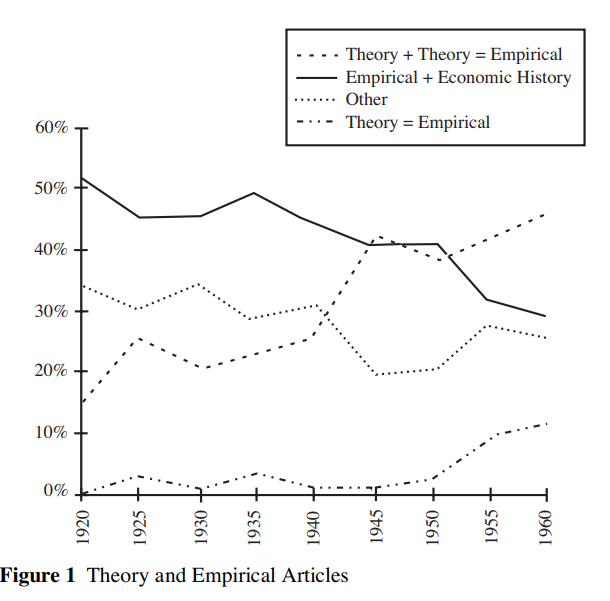
\includegraphics[width=0.75\textwidth]{4º Período/História do Pensamento Econômico/Tradução HPE/Tradução Tópico 7.2/figure 1.png}
    \end{figure}


A teoria formal se tornou, como se esperava, mais importante. Igualmente importante, no entanto, é uma mudança substancial, que não é quantificada, no estilo de escrita dos artigos de economia. Um economista que escrevia na década de 1920 normalmente construía argumentos lógicos que se pensava corresponderem de perto a circunstâncias específicas. Embora esses argumentos fossem em certo sentido teóricos, eles não foram separados das discussões empíricas. Assim, as mudanças mostradas na figura 1 não devem ser interpretadas para significar que a teoria deslocou o trabalho empírico puro, mas devem ser vistas como refletindo o surgimento de um estilo diferente de argumentação no qual o trabalho teórico pode ser distinguido do trabalho empírico. As categorias da economia moderna, difíceis de aplicar na década de 1920, tornaram-se progressivamente mais aplicáveis.

 \begin{figure}[H]
    \centering
    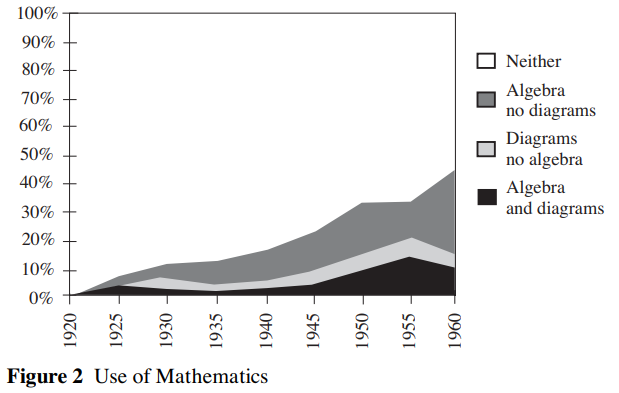
\includegraphics[width=0.75\textwidth]{4º Período/História do Pensamento Econômico/Tradução HPE/Tradução Tópico 7.2/figure 2.png}
    \end{figure}

O Uso da Matemática

Um aspecto importante desse processo foi o aumento do uso da matemática na economia, como mostrado na figura 2. Embora a matemática seja, em princípio, difícil de definir, as categorias usadas aqui eram inequívocas. O número de artigos que usavam algum tipo de matemática aumentou de zero em 1920 para 40 por cento em 1960. No entanto, a figura 2 subestima o aumento do uso da matemática em um sentido importante, pois o principal uso da matemática durante esse período está no desenvolvimento de argumentos teóricos. A matemática, além da análise estatística, raramente é usada no trabalho empírico. Como mostra a figura 3, a proporção de artigos teóricos que usavam álgebra aumentou muito mais rapidamente, atingindo quase 80 por cento em 1960. A figura 3 também confirma a visão comumente aceita de que, nas décadas de 1920 e início dos anos 1930, a AER era notavelmente menos matemática do que a QJE ou a JPE. Enquanto a matemática se estabeleceu na QJE e na JPE na década de 1920, não foi até a década de 1930 que isso aconteceu com a AER. No entanto, houve uma clara convergência em meados da década de 1950, quando uma proporção muito semelhante de artigos teóricos em todas as três revistas usava álgebra.

 \begin{figure}[H]
    \centering
    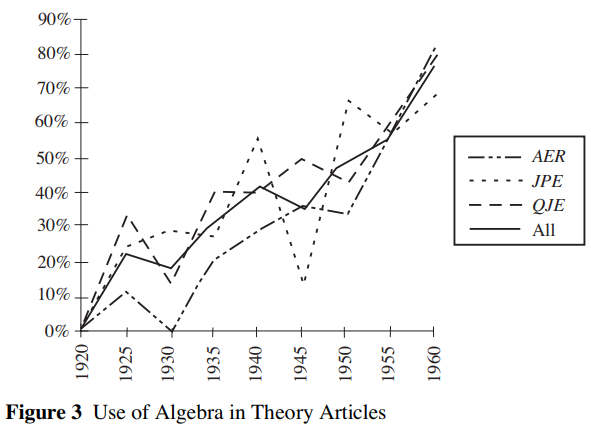
\includegraphics[width=0.75\textwidth]{4º Período/História do Pensamento Econômico/Tradução HPE/Tradução Tópico 7.2/figure 3.png}
    \end{figure}

Técnicas Empíricas

A econometria é comumente vista como tendo início nas décadas de 1920 e 1930 com o trabalho de Henry Schultz e Holbrook Working. A pesquisa revela, no entanto, que esses indivíduos contribuíram com uma grande proporção do trabalho de 1920 a 1960 que poderia ser classificado como econometria. A Tabela 1 mostra o número total de artigos usando análise de regressão (definida como envolvendo estatísticas diagnósticas) ou estatísticas descritivas que foram além de somas, médias, diferenças e similares (por exemplo, desvios padrão, análise de variância). Os números são realmente muito baixos.

Um indicativo de que essa amostra pode subestimar a aparência da econometria, como o termo é agora entendido, é fornecido na figura 4, que mostra a proporção de artigos empíricos na AER que usaram análise de regressão. Os anos na amostra de todas as revistas acontecem de ser anos em que a AEA publicou um número incomumente pequeno de artigos usando análise de regressão. No entanto, a Figura 4 confirma a imagem geral de que a análise de regressão começou a se estabelecer como uma ferramenta para pesquisa empírica na década de 1950. Muito mais comum era o uso de tabelas de estatísticas ou gráficos. A proporção de artigos que usaram gráficos ou tabelas aumentou de cerca de 50 por cento na década de 1920 para mais de 60 por cento em 1955-60.

\begin{figure}[H]
    \centering
    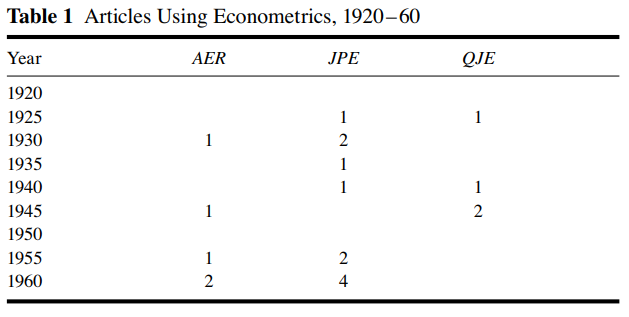
\includegraphics[width=0.75\textwidth]{4º Período/História do Pensamento Econômico/Tradução HPE/Tradução Tópico 7.2/table 1.png}
    \end{figure}

\begin{figure}[H]
    \centering
    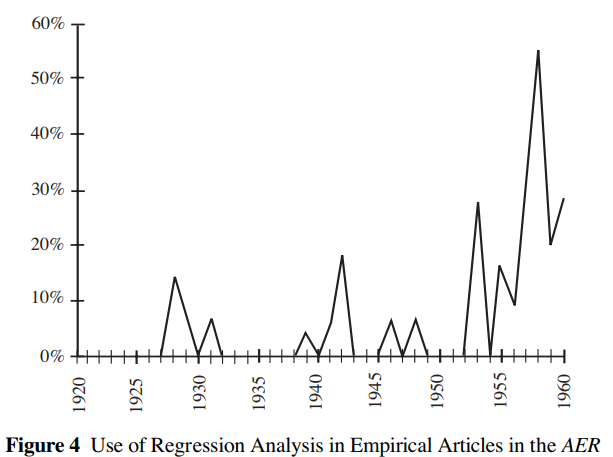
\includegraphics[width=0.75\textwidth]{4º Período/História do Pensamento Econômico/Tradução HPE/Tradução Tópico 7.2/figure 4.png}
    \end{figure}

\begin{figure}[H]
    \centering
    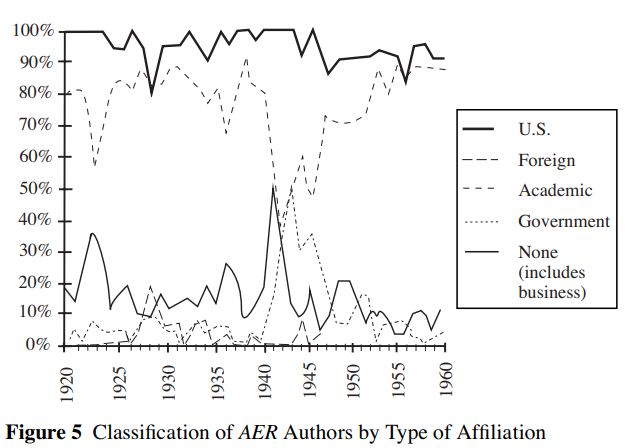
\includegraphics[width=0.75\textwidth]{4º Período/História do Pensamento Econômico/Tradução HPE/Tradução Tópico 7.2/figure 5.png}
    \end{figure}

\subsubsection{\textbf{Autores de Artigos de Revistas}}
Nacionalidade e Afiliação

As informações sobre os autores dos artigos do estudo são limitadas, mas ainda assim reveladoras. A Figura 5 classifica os autores da AER por tipo de afiliação. As afiliações dadas na revista são classificadas por país e por tipo de instituição. As categorias mais importantes são acadêmicas (universidades e institutos de pesquisa) e governamentais. A categoria rotulada como "nenhuma" inclui artigos para os quais nenhuma afiliação foi dada e um número muito pequeno que deu o nome de um negócio. A figura mostra que os artigos na AER foram esmagadoramente escritos por economistas baseados em instituições acadêmicas nos Estados Unidos. O contraste com as duas principais revistas britânicas examinadas em Backhouse 1997, que continham números significativos de artigos de economistas baseados fora da Grã-Bretanha, é marcante. Houve um breve aumento no número de contribuidores estrangeiros para a AER no final da década de 1920 e outro aumento para cerca de 10 por cento no final da década de 1940 e 1950. Igualmente significativa é a tendência de declínio no número de contribuidores para os quais nenhuma afiliação foi fornecida (a maioria dos quais eram presumivelmente não acadêmicos ou aposentados).

O principal evento subjacente à figura 5 é claramente a Segunda Guerra Mundial. Um grande número de economistas acadêmicos entrou para o serviço governamental durante a década de 1940, e depois retornou à academia após o fim da guerra. Embora houvesse exceções, como um artigo em 1943 sobre a curva de demanda de oligopólio vincada por Clarence Efroymson no Conselho de Produção de Guerra, praticamente todos os artigos eram sobre tópicos aplicados relevantes para a instituição onde o economista trabalhava. Assim, economistas do Office of Price Administration escreveram sobre controles de preços e a lacuna inflacionária, e economistas do Tesouro, do Bureau of the Budget e do Federal Reserve System escreveram sobre tributação, dívida governamental e política monetária. Uma das contribuições teóricas foi "‘Burden of the Debt’ and the National Income" (1944), de Evesey Domar, publicado enquanto Domar estava no Federal Reserve System. Em 1944-45, alguns artigos tentaram prever a renda nacional do pós-guerra.

Embora praticamente todos os contribuidores fossem baseados em instituições dos EUA, uma grande proporção nasceu no exterior. A Figura 6 classifica os autores da AER não por país de afiliação, mas por país de nascimento. Esta figura mostra um padrão notavelmente claro. Uma onda de imigração na década de 1920 foi revertida no início da década de 1930, seguida por um declínio dramático na proporção de contribuidores nascidos nos EUA para cerca de 50 por cento no final da década de 1940. Na década de 1950, a proporção se estabilizou em cerca de 70 por cento. Isso apoia a visão convencional de que a década de 1920 viu um influxo de emigrantes da Rússia e da Europa Oriental, e a década de 1930 viu migração em resposta à ascensão de Adolf Hitler na Alemanha. Embora esse influxo seja bem conhecido, a figura 6 mostra que ele tem um impacto muito significativo no fluxo de artigos sendo publicados que não se limitava a um pequeno número de indivíduos proeminentes, mas se estendia muito mais amplamente.

\begin{figure}[H]
    \centering
    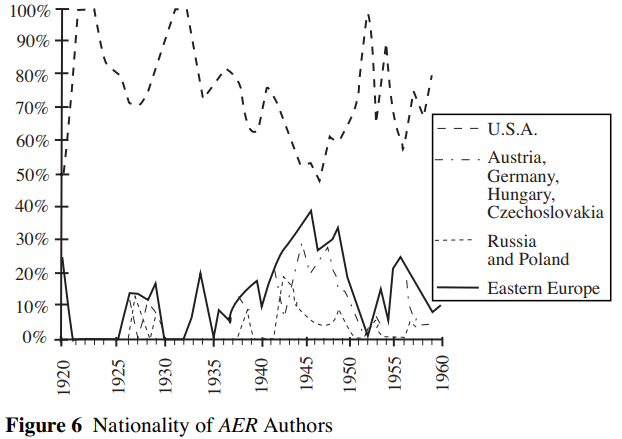
\includegraphics[width=0.75\textwidth]{4º Período/História do Pensamento Econômico/Tradução HPE/Tradução Tópico 7.2/figure 6.png}
    \end{figure}

Idade

Foi argumentado, notavelmente por Samuelson, que a transformação da economia que ocorreu nas décadas de 1930 e 1940 envolveu uma mudança geracional. Os jovens adotaram a economia matemática e a economia keynesiana de uma maneira que os economistas mais velhos não fizeram. Se isso estiver correto, deveríamos encontrar uma mudança na distribuição de idade dos colaboradores dessas revistas, especialmente entre os autores de artigos que usam matemática e artigos sobre macroeconomia. A Figura 7 mostra as idades médias dos colaboradores, e a Figura 8 mostra a distribuição de idades na amostra de cinco anos. A idade média era de cerca de 40 anos, aumentando ligeiramente ao longo do período. No entanto, houve variações notáveis na distribuição de idade. Não houve tendência na proporção de economistas com menos de 40 anos, mas a partir de 1945 em diante, houve uma queda na proporção de economistas com menos de 35 anos e, ainda mais dramaticamente, aqueles com menos de 30 anos contribuindo para essas revistas. Poderia ser argumentado que isso reflete a crescente profissionalização da disciplina e as crescentes demandas técnicas do assunto. Essas revistas estavam começando a ser consideradas prestigiosas, e os artigos nelas cada vez mais usavam matemática, o que dava uma vantagem aos economistas em seus trinta e poucos anos. Certamente não havia evidências de um influxo de jovens economistas nessas revistas na década de 1930.

\begin{figure}[H]
    \centering
    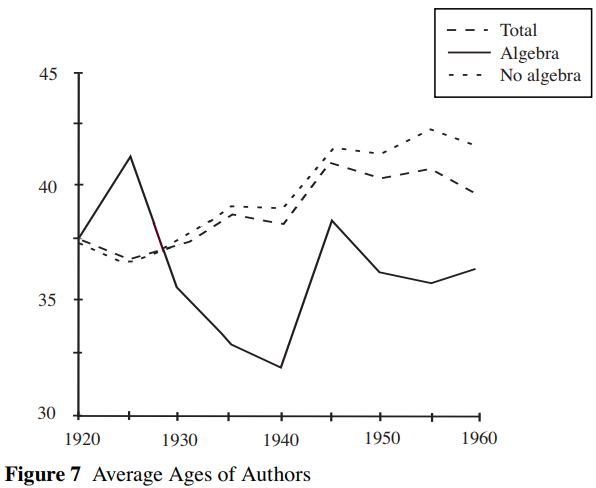
\includegraphics[width=0.75\textwidth]{4º Período/História do Pensamento Econômico/Tradução HPE/Tradução Tópico 7.2/figure 7.png}
    \end{figure}

\begin{figure}[H]
    \centering
    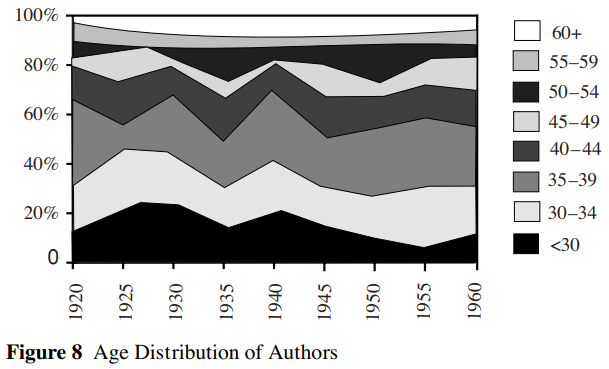
\includegraphics[width=0.75\textwidth]{4º Período/História do Pensamento Econômico/Tradução HPE/Tradução Tópico 7.2/figure 8.png}
    \end{figure}

De muito mais interesse é o padrão de idade dos autores de artigos que usam álgebra. Não há evidências de que os economistas matemáticos na década de 1920 e na primeira metade da década de 1930 eram mais jovens do que a média (embora deva ser lembrado que a amostra é pequena), mas durante meados a final da década de 1930 surgiu uma grande lacuna: em 1940 - 44 os economistas matemáticos tinham em média trinta e dois anos, sete anos mais jovens do que os autores de artigos que não usavam álgebra. Durante o final da década de 1940, essa lacuna fechou acentuadamente, com a idade média dos economistas matemáticos subindo para trinta e oito. A partir de 1950, a lacuna se estabilizou em cerca de cinco anos. Isso é consistente com a teoria de que a economia matemática foi introduzida por uma nova geração que entrou na profissão no final da década de 1930. O aumento na idade dos economistas matemáticos no final da década de 1940 apoia essa teoria, pois nesse período os entrantes na profissão normalmente teriam sido mais velhos, tendo passado vários anos nas forças armadas. O aumento na idade média dos usuários de álgebra na década de 1950 em comparação com a idade média no final da década de 1930 e início da década de 1940 pode ser explicado pelas crescentes demandas técnicas do assunto e pelo fato de que essas técnicas estavam se tornando muito mais amplamente aceitas.

\subsubsection{\textbf{Instituições}}
A análise das afiliações institucionais dos autores pode lançar luz sobre dois fenômenos: o domínio de um pequeno número de instituições e as mudanças nas instituições líderes à medida que o assunto foi transformado. Na medida em que as instituições estão associadas a abordagens particulares da economia (Wisconsin com institucionalismo, o Instituto de Tecnologia de Massachusetts [MIT] com economia neoclássica), isso pode nos ajudar a documentar a transformação do assunto. No entanto, muitas instituições não podem ser associadas a escolas de pensamento específicas. De 1925/26 a 1950/51, os principais produtores de Ph.D. em economia foram Harvard (600), Columbia (394), Wisconsin (282), Cornell (244), Chicago (243) e Illinois (218) (Bowen 1953, citado em Moggridge 1995). Desses, Columbia tinha uma forte presença institucionalista (Clark e Mitchell), mas Harold Hotelling também estava lá fazendo economia matemática, embora Arrow (1990, 46) afirme que até 1940, quando era estudante, a ênfase do Departamento de Economia "era quase inteiramente em análises empíricas e institucionais". Thorstein Veblen estava em Chicago no início do período, e Knight estava lá no final. Harvard também não pode ser facilmente associada a uma única escola: Taussig, Chamberlin e Schumpeter claramente não eram institucionalistas, mas também não eram neoclássicos. Além de Samuelson, Harvard produziu John Kenneth Galbraith.

As instituições podem ser analisadas considerando-se as instituições nas quais os autores estavam baseados quando seus artigos foram publicados ou vinculando os autores às instituições das quais se formaram, definidas aqui como a instituição da qual um Ph.D. foi obtido. Os dados são mostrados nas tabelas 2 e 3. A amostra da AER foi escolhida para evitar o viés em direção a Chicago e Harvard que resultaria do uso do JPE e do QJE.

A Tabela 2 mostra pouca mudança no grau de concentração de afiliação. Em todas as décadas, exceto a década de 1940, as três principais instituições representavam cerca de 15 por cento dos artigos, as dez primeiras por volta de 38 por cento, e as quinze primeiras por volta de 45 por cento. A década de 1940 viu uma redução na concentração, talvez porque um número desproporcional de economistas publicadores de instituições líderes foram atraídos para o trabalho de guerra. Seja qual for a razão, as proporções de concentração do pré-guerra foram restabelecidas na década de 1950.

A história em relação às instituições de Ph.D. é mais mista, embora o que se destaca é o grau muito maior de concentração. As três principais instituições de Ph.D. representaram quase 50 por cento dos artigos, as dez primeiras por volta de 75 por cento, e as quinze primeiras por mais de 80 por cento. Se a formação de Ph.D. é importante para determinar a direção do assunto, é necessário considerar apenas um número muito pequeno de instituições.

Embora o sistema fosse altamente concentrado, houve mudanças notáveis nas instituições dominantes, como mostrado em ambas as tabelas. Nas três primeiras décadas do período, economistas baseados em Princeton, Columbia e Harvard dominaram a AER, enquanto na década de 1950 as instituições líderes eram Berkeley, MIT e Stanford. Também é digno de nota o aumento constante de Chicago para o quarto lugar na década de 1950. Tendo em vista o declínio do institucionalismo, muitas vezes datado da década de 1930, é significativo que Wisconsin tenha caído de cerca de sétimo lugar na década de 1920 para o décimo primeiro na década de 1950. No entanto, o declínio na participação de artigos da AER por Ph.D.s de Wisconsin é ainda mais acentuado, de 12 por cento na década de 1920 e 10 por cento na década de 1930 para apenas 5 por cento na década de 1950. Nas décadas de 1940 e 1950, a AER foi dominada por economistas treinados em Harvard, que escreveram tantos artigos quanto economistas das duas próximas instituições, Columbia e Chicago, combinados. Na década de 1920 e 1930, Ph.D.s de Harvard e Columbia publicaram artigos da AER em números iguais na década de 1950.

\begin{figure}[H]
    \centering
    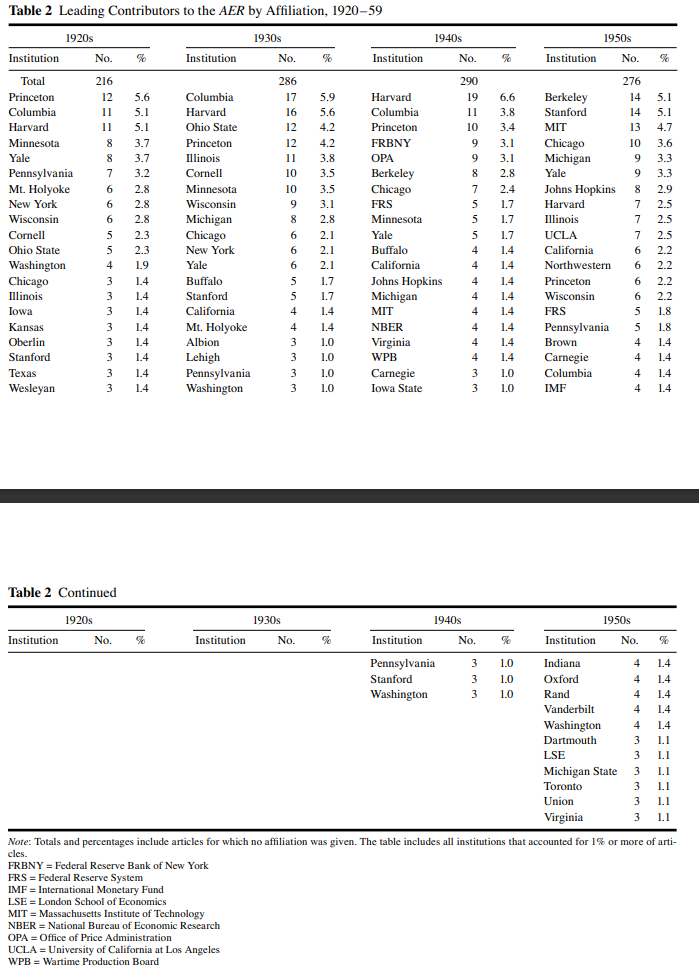
\includegraphics[width=0.75\textwidth]{4º Período/História do Pensamento Econômico/Tradução HPE/Tradução Tópico 7.2/table 2.png}
    \end{figure}

\begin{figure}[H]
    \centering
    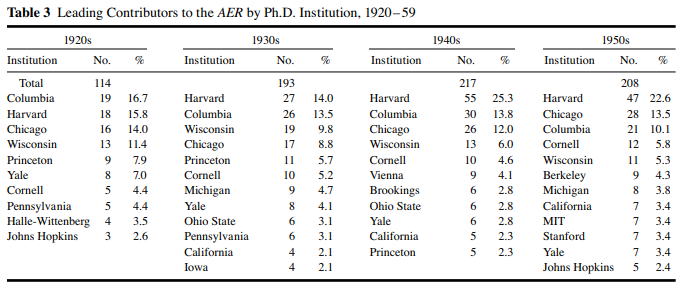
\includegraphics[width=0.75\textwidth]{4º Período/História do Pensamento Econômico/Tradução HPE/Tradução Tópico 7.2/table 3.png}
    \end{figure}

\subsubsection{\textbf{Conclusão}}
A análise da economia dos EUA confirma muitas das histórias que contamos sobre a transformação da economia entre 1920 e 1960. Imigrantes da Europa tiveram um impacto quantitativo significativo, indo além da influência de um pequeno número de indivíduos proeminentes. As evidências apoiam a ideia de que a década de 1930 foi um período crucial na matematização do assunto, associada ao influxo de uma geração mais jovem de economistas. A econometria, como o termo é agora entendido, no entanto, não decolou até a década de 1950. Embora as evidências estejam longe de ser conclusivas, é possível ver padrões que são consistentes com o declínio do institucionalismo começando na década de 1930: a participação decrescente de artigos da AER produzidos de Wisconsin e por Ph.D.s de Wisconsin; o surgimento repentino de Stanford, MIT e Berkeley na década de 1950; e possivelmente o deslocamento de Columbia por Harvard. Isso é o que a maioria das pessoas esperaria.

A análise também sugere algumas características da transformação da economia dos EUA que de outra forma poderiam ter sido esquecidas. O impacto massivo da guerra na profissão é o mais óbvio. Em um momento crucial, um grande número de economistas deixou a academia para trabalhar no governo ou no exército. Igualmente importante, a matematização do assunto, embora tenha avançado muito, estava longe de estar completa em 1960. Se a ortodoxia dominante é vista como envolvendo o uso de modelos de otimização formal que são testados usando técnicas econométricas, o assunto ainda tinha um longo caminho a percorrer. Por exemplo, até 1960, 71 por cento dos artigos empíricos não usavam análise de regressão. O aumento dramático de 1955 a 1960 na proporção de artigos que usavam álgebra, mas nenhum diagrama, sugere que uma mudança substancial estava ocorrendo justamente quando o período terminava. Esta é uma característica da transformação da economia dos EUA que as contas de figuras-chave, como Arrow, Samuelson ou Friedman, podem facilmente ignorar.

No entanto, uma das conclusões mais significativas surge não da análise estatística, mas da classificação dos artigos. O fato de que era difícil classificar muitos artigos da primeira metade do período como teóricos ou empíricos, mas menos difícil em direção ao final do período, é uma evidência de que uma mudança significativa ocorreu na economia dos EUA durante esse período. Embora a mudança tenha sido indubitavelmente associada à transformação da economia dos EUA do pluralismo pré-guerra para o neoclassicismo pós-guerra - pois a divisão entre teórica e empírica é uma característica do tipo de economia que tem cada vez mais dominado o assunto no período pós-guerra - ela não é sinônima com isso. A economia acadêmica estava se expandindo, juntamente com todo o sistema de educação superior, e o assunto estava cada vez mais capaz de apoiar uma variedade de revistas, como as discutidas aqui, lidando com questões que eram de preocupação principalmente apenas para economistas acadêmicos. A economia estava se tornando, juntamente com muitas outras disciplinas, mais voltada para dentro. Ambas as técnicas teóricas e empíricas se tornaram mais formais, permitindo que fossem distinguidas uma da outra de uma maneira que não era possível na década de 1920.


\section{\textbf{(OPCIONAL) : Claveau e Gingras (2016)}}
\subsection{\textbf{Macrodinâmica da Economia: Uma História Bibliométrica}}
As disciplinas acadêmicas cresceram enormemente desde a Segunda Guerra Mundial e a economia não é exceção. Entre os artigos de economia indexados na Web of Science da Thomson Reuter, cerca de mil foram publicados em 1956, enquanto quase vinte mil são publicados anualmente hoje. Esse aumento equivale a uma taxa de crescimento anual média entre 5 e 6 por cento, que é comparável ao crescimento anual global da ciência no mesmo período (Larsen e von Ins 2010). Para ter certeza, esses números dão apenas uma indicação aproximada do crescimento da economia, porque a Web of Science não indexa todos os artigos acadêmicos, mas apenas um subconjunto que aparece nas principais revistas acadêmicas ao redor do mundo. No entanto, esses números aproximados são suficientes para indicar a magnitude das transformações que afetaram a escala da pesquisa científica em geral e em economia em particular ao longo do último meio século.

Embora os tipos tradicionais de análise do desenvolvimento da economia - análise textual de documentos e arquivos publicados, entrevistas, reconstrução biográfica de figuras importantes, genealogia de conceitos e métodos - permaneçam úteis, ferramentas específicas valem a pena explorar para entender a estrutura global e morfologia da economia à medida que mudou ao longo da segunda metade do século XX. Este artigo introduz uma combinação dessas ferramentas para a história da economia. Combinamos bibliometria com análise de rede dinâmica para identificar uma estrutura de especialidade em mudança na economia desde o final dos anos 1950 até 2014. Mapeamos como as especialidades surgiram, cresceram em relação umas às outras e (para algumas delas) desapareceram. Nossos resultados se combinam bem com relatos mais narrativos da história recente da economia (por exemplo, Backhouse 2002, cap. 14; Backhouse e Cherrier 2014; e Morgan e Qin 2015): eles confirmam certas afirmações que podem ser encontradas na literatura existente e identificam padrões intrigantes que convidam a uma pesquisa qualitativa mais aprofundada (veja a seção 5)

Dados bibliométricos têm sido usados na economia, mas essencialmente para estatísticas descritivas com fins avaliativos - por exemplo, classificações de revistas e autores mais citados (Kalaitzidakis, Mamuneas e Stengos 2003; Kodrzycki e Yu 2006; Ritzberger 2008; Stern 2013; Zimmermann 2013; Card e DellaVigna 2013). Apenas alguns artigos que usam dados bibliométricos da economia não têm um objetivo avaliativo explícito, concentrando-se mais na estrutura da autoria e nos métodos usados em artigos em um pequeno número de chamadas revistas de topo (Hamermesh 2013), na identificação das características dos artigos mais citados (Kim, Morse e Zingales 2006), ou na descrição da evolução do número de artigos em um determinado domínio de pesquisa (por exemplo, Silva e Teixeira 2008; Silva e Teixeira 2009).

Até onde sabemos, este artigo é o primeiro no campo da história da economia a combinar dados bibliométricos e análise de rede dinâmica. Além disso, nosso corpus de cerca de 415.000 documentos é muito maior do que os corpora usados na maioria dos outros estudos sobre a história da economia. O artigo segue os passos de vários estudos que mostraram que a bibliometria e a análise de rede são particularmente adequadas para estudos de grande escala do desenvolvimento histórico de disciplinas científicas e especialidades (Garfield 2009; Cole, Cole e Dietrich 1978; Boyack, Börner e Klavans 2009; Gingras 2010a, 2010b, 2010c; Gingras e Schinckus 2012). A grande vantagem de combinar bibliometria e análise de rede é a possibilidade de detectar e visualizar algoritmicamente padrões na produção de pesquisa de grandes grupos. Padrões que podem permanecer ocultos ou embaçados com métodos históricos padrão de repente vêm à luz.

\subsubsection{\textbf{1. Estrutura Conceitual: Economia como uma Rede de Especialidades}}

Em qualquer disciplina científica madura, a comunidade científica é de fato composta de subunidades relativamente autônomas (as especialidades) nas quais o novo conhecimento é tornado público por meio de publicações. Essas diferentes especialidades, que surgiram ao longo do tempo com o crescimento morfológico e a subsequente divisão do trabalho dentro da disciplina, estão mais ou menos conectadas entre si, assim como a própria disciplina está mais ou menos conectada a outras disciplinas que compõem o campo científico global. Enquanto a disciplina geralmente corresponde ao treinamento básico de nível de entrada (BA) em um departamento universitário, a especialidade corresponde mais ao nível de pesquisa aprendido nos níveis de mestrado e doutorado e leva à produção de novos conhecimentos (Hagstrom 1965; Cole e Cole 1973; Whitley 1976; Whitley 2000; Bourdieu 2004; Wray 2005).

\newpage
\section*{\textbf{Tópico 8.1}}
\addcontentsline{toc}{section}{Tópico 8.1}
\section{\textbf{Morgan (2008)}}
\subsection{\textbf{Classificação JEL B4}}
A modelagem se tornou a metodologia dominante da economia durante o século 20.

No entanto, apesar de seu uso onipresente na economia moderna, o termo 'modelo' foi introduzido relativamente recentemente. No final do século 19, os 'modelos' nem sequer eram uma categoria reconhecida nas discussões sobre metodologia (como por exemplo no Dicionário de Economia Política de Palgrave dos anos 1890), embora alguns existissem como objetos de trabalho práticos. O uso efetivo do termo 'modelo' na economia está associado ao movimento de econometria do período entre guerras, um movimento cujo objetivo era tanto desenvolver quanto fundir abordagens matemáticas e estatísticas para a economia. Dessa noção original ampla, na década de 1950 surgiram campos separados de economistas matemáticos e econométricos, e ambos mantiveram a modelagem como uma ferramenta central de sua prática científica. Tornou-se convencional então pensar em modelos na economia moderna como objetos matemáticos usados na teoria econômica ou como objetos econométricos (envolvendo propriedades estatísticas e matemáticas) no trabalho empírico. As contas históricas de modelos na economia moderna podem começar convenientemente então com essa divisão.

Os comentários filosóficos, também, na maioria das vezes tendem a seguir essa divisão, tratando os modelos da teoria econômica como diferentes tipos de criaturas, com diferentes papéis, daqueles que são aplicados aos dados. O último papel dos modelos, o de 'adequar teorias ao mundo', é exemplificado na modelagem empírica, no trabalho econométrico e nas declarações metodológicas de Jan Tinbergen na década de 1930. Em contraste, os modelos matemáticos da economia moderna são vistos principalmente como uma maneira pela qual a construção da teoria econômica acontece. Essa visão de 'modelagem como teorização' é exemplificada nas declarações programáticas de Tjalling Koopmans em 1957. Um terceiro quadro metodológico apresenta 'modelos como instrumentos de investigação': ferramentas para aprender sobre a teoria econômica ou o mundo econômico, uma posição tipificada no trabalho de Irving Fisher no final do século 19 e início do século 20, que pode ser visto como outro dos fundadores da modelagem na economia.

Este artigo aborda o surgimento histórico e os papéis dos modelos na economia de acordo com essas três diferentes contas metodológicas, e discute como essas abordagens se encaixam na ciência econômica moderna.

\subsection{\textbf{Modelagem como Ajuste de Teorias ao Mundo}}
Embora uma vibrante comunidade de econometria tenha se desenvolvido nas duas décadas até a década de 1920, seus produtos (regressões de demanda, contas estatísticas de ciclos de negócios e assim por diante) foram apresentados como descrições diretas das relações econômicas subjacentes, em vez de como modelos propostos de forma tentativa para representá-los (veja Morgan 1990). A diferença é sutil, mas iluminada pelo uso do termo 'econométrico natural' de Philippe Le Gall (2007) para aqueles economistas do século 19 que acreditavam, em paralelo às ciências naturais, que as leis que governavam a economia eram escritas em matemática, e a manipulação inteligente de dados estatísticos (sem, deve-se dizer, muito em termos de técnicas analíticas) revelaria essas leis.

Nesse quadro estatístico descritivo, Jan Tinbergen não apenas introduziu o termo 'modelo' em 1935 (veja Boumans 1993), mas também foi responsável - juntamente com Ragnar Frisch - pelo desenvolvimento de tais objetos matemático-estatísticos na econometria da década de 1930. (Antes disso, o raro uso do termo 'modelo' normalmente se referia a modelos de objetos físicos como Boltzmann os definiu em 1911. Paul Ehrenfest é a provável fonte de uma ampliação no escopo do termo para incluir modelos matemáticos, e Tinbergen foi seu assistente durante a metade da década de 1920; veja Boumans 2005, cap. 2.) Frisch em 1933 desenvolveu - no contexto da pesquisa de ciclo de negócios - a noção de um 'esquema macrodinâmico': um modelo de três equações com erros aleatórios. Ele até simulou para mostrar que poderia reproduzir as características genéricas dos dados de séries temporais de seu tempo. Mas foi Tinbergen quem desenvolveu o design de Frisch em um modelo econométrico - um modelo que poderia ser ajustado aos dados reais da economia. Como é bem conhecido, ele construiu a primeira geração de modelos macroeconométricos (veja Tinbergen 1937; 1939; e Bodkin et al. 1991), e ao fazer isso ele tornou explícita a noção de um modelo como um veículo para preencher a lacuna entre teorias do ciclo de negócios e dados estatísticos específicos (tempo e lugar) do ciclo, como Morgan (1990, cap. 4) argumenta. Para apreciar a tarefa, é preciso lembrar que a maioria das teorias existentes do ciclo era expressa verbalmente, e as teorias matemáticas nascentes do ciclo eram muito pequenas e simplificadas para representar as características dos ciclos reais, então até mesmo construir um sistema de equações a partir dessas teorias era uma tarefa considerável. Os dados também desempenharam um papel na decisão da sequência temporal das relações e quais variáveis deveriam ser incluídas ou omitidas, pois ambos esses elementos foram determinados no trabalho estatístico. Em outras palavras, Tinbergen criou um conjunto de relações matemático-estatísticas utilizáveis que incorporavam tanto ideias teóricas sobre como a economia funcionava quanto representavam empiricamente as diferentes partes da economia. Tendo ajustado teorias e dados juntos no formato do modelo econométrico, ele então usou o modelo para testar a viabilidade de várias teorias do ciclo, para explicar eventos na economia e para executar o modelo para a frente com diferentes opções de política relevantes para os anos da Grande Depressão - tudo isso na era pré-computador usando calculadoras manuais! Essa 'nova prática' de modelos, como Boumans (2005) a denomina, envolveu uma construção criativa da teoria econômica matemática em relação aos dados estatísticos do mundo econômico e da habilidade artesanal no uso desses modelos. Para Frisch e Tinbergen, a modelagem era um projeto para explicar como o mundo econômico funcionava.

A próxima etapa na história pode ser marcada pelo famoso plano de Trygve Haavelmo para a econometria de 1944, que trouxe outra mudança sutil de foco para a tarefa de modelagem econométrica. Ele sugeriu que a econometria deveria se preocupar, não com um processo de correspondência entre teoria e dados em um processo iterativo, mas com a busca do modelo correto para os dados observados usando raciocínio de probabilidade (veja Morgan 1990, cap. 8). Ele efetivamente introduziu na econometria não apenas a noção do modelo teórico (o modelo matemático derivado da teoria a priori), mas também a do modelo 'verdadeiro' (mas desconhecido): 'o mecanismo 'verdadeiro' sob o qual os dados considerados estão sendo produzidos' (Haavelmo 1944, p. 49). No entanto, ele estava longe de ser um 'econométrico natural' (no sentido de Le Gall para o século 19), argumentando sobre modelos de comportamento econômico que 'seja qual for as 'explicações' [dos fenômenos econômicos] que preferimos, não deve ser esquecido que todos são nossas próprias invenções artificiais em busca de uma compreensão da vida real; eles não são verdades ocultas a serem "descobertas"' (Haavelmo 1944, p. 3). Embora ele tenha insistido que um modelo econométrico bem ajustado (uma teoria que se ajusta bem aos dados) pode não ser o modelo 'verdadeiro', no entanto, sua abordagem de probabilidade de plano foi destinada a alterar a tarefa aceita de econometria. A abordagem da Comissão Cowles que se seguiu (cujas contribuições são analisadas por Qin 1993, e Epstein 1987) enfatizou o uso dos métodos corretos de identificação e estimação do modelo estrutural completo derivado teoricamente como o meio de descobrir esse modelo verdadeiro. O 'apriorismo forte' de sua abordagem para a econometria, na qual a teoria propõe o modelo e os dados dispõem (ou não) dessas hipóteses, provocou o famoso debate 'medição sem teoria' com o ramo mais empirista do campo sobre como fazer econometria no final da década de 1940.

É tentador ver a provisão de Haavelmo de uma base filosófica para a econometria como pavimentando o caminho para uma divisão de trabalho pós-1950 no uso de modelos - ou seja, os economistas fornecem modelos matemáticos da teoria econômica, e o trabalho do econométrico é usar estatísticas para estimativa de modelos e teste de teorias. Até certo ponto, essa divisão de trabalho é confirmada, pois é neste período que surge uma distinção muito mais clara entre economia teórica e aplicada (como visto em Backhouse 1998). No entanto, apesar da retórica da econometria pós-1950 que fala de 'confrontar teoria com dados', ou 'aplicar teoria aos dados', do ponto de vista da modelagem econométrica, a divisão prática não é tão clara. Existem várias razões. Primeiro, permanece um comentário prosaico, mas geralmente válido, que a teoria raramente fornece todos os recursos necessários para fazer modelos que podem ser imediatamente aplicados aos dados do mundo. É precisamente por isso que os modelos econométricos se destacaram como um intermediário necessário, um dispositivo de correspondência, entre eles. Segundo, esse processo de correspondência de ajustar teorias ao mundo é feito com muitos propósitos diferentes - para testar teorias, para medir relações, para explicar eventos, e assim por diante - cada um precisando de recursos diferentes da teoria e com critérios diferentes. Terceiro, não existem regras científicas gerais para modelagem. Houve argumentos acirrados dentro da comunidade de econometria nas últimas décadas sobre vários princípios científicos para modelagem (e critérios associados): se os modelos devem ser orientados pela teoria ou orientados pelos dados; se o processo de modelagem deve ser simples para geral ou geral para específico; e assim por diante (veja Pagan 1987; Heckman 2000). Independentemente de quais princípios são seguidos, o elemento criativo ainda é muito evidente onde quer que ocorra a modelagem econométrica aplicada, seja essa modelagem no extremo de busca de padrões ou modelagem orientada pela teoria, e seja o campo macro ou microeconométrico.

Uma mudança de foco mais recente, particularmente no campo macroeconométrico e associada a Robert Lucas, implica em desistir do objetivo de usar a teoria para fazer modelos que representem a verdadeira estrutura geral como uma maneira de descobrir essa estrutura. Como ele escreveu:

Uma 'teoria' não é uma coleção de afirmações sobre o comportamento da economia real, mas sim um conjunto explícito de instruções para construir um sistema paralelo ou análogo - uma economia de imitação mecânica. Um 'bom' modelo, deste ponto de vista, não será exatamente mais 'real' do que um pobre, mas fornecerá melhores imitações. (Lucas 1980, p. 697)

Essa mudança altera a relação entre modelos e teoria, pois agora a tarefa da teoria é produzir modelos como analogias do mundo, em vez de usá-los para explicar o comportamento do mundo (veja Boumans 1997). Ao mesmo tempo, muda o foco do 'ajuste': o objetivo não é mais ajustar a teoria ao mundo, mas ajustar o modelo ao mundo no sentido particular de ser capaz de imitar certos tipos de características de dados.

Outra conta recente, desenvolvida desta vez na microeconometria por John Sutton (2000), se valida em relação à agenda econométrica anterior mantida por Frisch e Tinbergen, pois, como esses pioneiros iniciais, ele pensa em modelos não como dispositivos para a descoberta do modelo geral verdadeiro como na interpretação da Comissão Cowles do projeto de Haavelmo, nem como máquinas matemáticas que imitam o mundo como na conta de Lucas, mas como dispositivos investigativos para descobrir sobre o mundo. Na visão de Sutton, o mundo econômico produz regularidades ou variabilidades razoavelmente estáveis apenas dentro de uma classe de casos, não em todos os casos; portanto, procurar um modelo geral é muito ambicioso. O objetivo da modelagem é descrever os mecanismos econômicos que produzem as características dos dados que são compartilhadas dentro de um subconjunto de todos os casos e, assim, explicar as regularidades observadas dentro dessa subclasse. Sutton descreve isso como uma abordagem de 'classe de modelos'. Mais uma vez, os modelos aparecem como um dispositivo intermediário entre a teoria e os dados, mas desta vez funcionam para classificar casos semelhantes no mundo e, assim, oferecer explicações para seu comportamento característico.

Os modelos aparentemente desempenham um papel epistemológico crítico na econometria - mas existem diferentes maneiras de caracterizar isso. A econometria pode ser vista como cumprindo a função de experimentos de laboratório em algumas outras ciências - uma afirmação que está implícita na discussão de Haavelmo sobre os dados da economia como sendo o resultado da observação passiva dos experimentos da natureza e explícita em sua discussão sobre modelagem econométrica como projetando experimentos (veja Haavelmo 1944, cap. 1 e 2). Sua conceituação de econometria apela para a importância da probabilidade e do raciocínio estatístico como as bases para o design do modelo e a inferência estatística: os modelos têm que ser projetados para corresponder aos dados que poderiam ser observados e ser enquadrados em termos de probabilidade. A noção de 'design de experimentos' requer que o econométrico pense sobre o problema de ajuste, enquanto a configuração de probabilidade dá regras para inferências a partir do experimento do modelo, que são de fato muito melhor especificadas do que aquelas para experimentos de laboratório na maioria das ciências. Assim, o plano de Haavelmo compra explicitamente uma tradição de pensamento estatístico como um modo válido de raciocínio científico, mas o reinterpreta como uma forma de trabalho experimental.

Uma caracterização mais recente da função epistemológica dos modelos em econometria é entendê-los como instrumentos de observação e medição que permitem aos economistas identificar fenômenos estáveis no mundo da atividade econômica. A conta de Kevin Hoover de 'econometria como observação' descreve 'cálculos econométricos' como 'o telescópio do economista' (1994, p. 74) onde as regras para focar o telescópio vêm da teoria estatística e onde a teoria econômica, e o propósito engajado, guiam o processo de observação. Marcel Boumans (2005) entende os modelos como o instrumento primário neste processo, sem o qual os economistas não poderiam 'modelar o mundo em número'. Em vez de um meio de observação, ele retrata os modelos como instrumentos científicos complexos que geram os números para aqueles objetos econômicos, conceitos e relações que não podem ser observados diretamente e que ainda não são medidos. Como Haavelmo, a conta de trabalho do modelo de Boumans invoca um design cuidadoso de experimentos, mas ele fornece uma discussão mais concreta de como a modelagem econométrica fornece estruturas de medição para lidar com cláusulas ceteris paribus; como critérios estatísticos e outros fornecem maneiras de avaliar a confiabilidade dos instrumentos do modelo (via calibração, filtragem e assim por diante); e como a precisão e o rigor são obtidos no processo de medição.

Nem Boumans nem Hoover são instrumentalistas sobre modelos no sentido que passou a ser associado ao argumento de Milton Friedman de 1953 de que os modelos precisam ser eficientes apenas para previsão, não para explicação. (O ensaio de Friedman tem sido muito discutido, e as interpretações deste ponto particular variam; veja particularmente Hirsch e De Marchi 1990; instrumentalismo e operacionalismo; e Mäki 2007.) Nem são operacionistas no sentido Bridgmaniano (que informou, por exemplo, o trabalho inicial de Paul Samuelson em economia; veja Bridgeman 1927), ou seja, que um conceito é definido por seu processo de medição (como um modelo econométrico). Tanto Hoover quanto Boumans podem ser chamados de 'instrumentalistas sofisticados' pois consideram cálculos econométricos ou modelos como instrumentos habilmente projetados para observar e medir as relações da economia, e assim entender e explicar, o mundo.

\subsection{\textbf{Modelagem como Teorização}}
O termo 'modelo' raramente foi usado em economia antes da década de 1930, embora coisas que agora rotularíamos como 'modelos' tenham sido desenvolvidas e usadas para teorizar antes disso. Podemos certamente reconhecer alguns exemplos anteriores de modelagem no final do século 19; por exemplo, podemos felizmente denotar o diagrama de caixa de Edgeworth-Bowley, e os diagramas de comércio e tesoura de oferta-demanda de Alfred Marshall como modelos. Esses exemplos sinalizam que a modelagem era um elemento não reconhecido no processo de matematização desse período anterior (veja Morgan 2008). No entanto, foi apenas depois da década de 1950 que a modelagem se tornou uma maneira amplamente reconhecida de usar matemática na economia e se tornou uma das formas dominantes de teorização econômica. Enquanto o estabelecimento da noção estatístico-econométrica está associado a Tinbergen, o matemático-teorizante pode estar associado a outro econométrico holandês, Tjalling Koopmans, cuja conta, dada em um conjunto de três ensaios em 1957, é amplamente entendida como uma declaração paradigmática da abordagem de modelagem da economia matemática moderna. Koopmans desenvolveu as ideias anteriores de Tinbergen sobre modelagem para se ajustar às discussões contemporâneas sobre o papel da matemática na economia nas décadas de 1940 e 1950 e com a ideia formal matemática de um modelo naquela época. Como tal, sua declaração se encaixa em uma história mais ampla de matemática e economia tratada particularmente em Weintraub (2002) e Ingrao e Israel (1987).

Koopmans definiu uma teoria econômica como um conjunto de postulados com os quais raciocinamos para elaborar e tornar explícitos os efeitos, de outra forma implícitos, do conjunto de postulados tomados em conjunto: uma prática de raciocínio que aparentemente envolve modelos. Para Koopmans, esse raciocínio era uma parte importante da teorização, uma vez que essas implicações não são autoevidentes, nem qualquer conjunto particular de postulados é necessariamente frutífero. Sua representação de 'Teoria Econômica como uma Sequência de Modelos' (para citar seu título de seção de 1957, p. 142) é apresentada como sua resposta ao argumento contínuo de seu dia sobre o status das suposições e as previsões da economia, no qual ele explicitamente definiu o papel dos modelos quase como um aparte:

nem os postulados da teoria econômica são totalmente autoevidentes [como Robbins argumentou em 1932], nem as implicações de vários conjuntos de postulados são prontamente testadas pela observação [como Friedman argumentou em 1953]. Nesta situação, é desejável que organizemos e registremos nossas deduções lógicas de tal maneira que qualquer conclusão ou implicação refutável observacionalmente possa ser rastreada até os postulados em que se baseia ... Considerações desta ordem sugerem que olhemos para a teoria econômica como uma sequência de modelos conceituais que buscam expressar em forma simplificada diferentes aspectos de uma realidade sempre mais complicada. A princípio, esses aspectos são formalizados tanto quanto possível isoladamente, depois em combinações de realismo crescente. (Koopmans 1957, p. 142)

Koopmans sugere, então, que os modelos são um elemento essencial na teorização, e que seu papel vem em sua capacidade sequenciada de expressar diferentes e combinados aspectos de uma realidade simplificada. Mas sua projeção de que tal sequência de modelos representaria 'combinações de realismo crescente' parece não ter se concretizado. Embora a tratabilidade sugira que o realismo crescente em alguns aspectos terá que ser compensado pela simplificação em outros, a história da modelagem sugere que as sequências de modelos são mais frequentemente impulsionadas por mudanças em problemas, em questões e nas ferramentas matemáticas disponíveis. Esta última foi uma possibilidade que o próprio Koopmans discute no contexto da mudança de formas de teorização aritmética para diagramática para algébrica. E, como acabamos de notar com Lucas, algumas modelagens modernas não visam mais representar o mundo como ele é, mas desenvolver sistemas artificiais que imitam as saídas do mundo.

Existem várias maneiras de caracterizar o uso de modelos matemáticos na teoria econômica. Para Daniel Hausman, a conexão dos modelos com a formação de conceitos é tanto mais explícita quanto mais importante do que Koopmans sugere, pois a modelagem econômica é onde o desenvolvimento da teoria acontece:

Uma teoria deve identificar regularidades no mundo. Mas a ciência não avança principalmente por identificar correlações entre várias propriedades conhecidas das coisas. Um passo absolutamente crucial é construir novos conceitos - novas maneiras de classificar e descrever fenômenos. Grande parte da teorização científica consiste em desenvolver e pensar sobre tais novos conceitos, relacioná-los a outros conceitos e explorar suas implicações.

Esse tipo de empreendimento é particularmente proeminente na economia, onde os teóricos dedicam muito esforço para explorar as implicações da racionalidade perfeita, informação perfeita e competição perfeita. Essas explorações, que são separadas de questões de aplicação e avaliação, são, acredito eu, o que os economistas (mas não os econométricos) chamam de 'modelos'. (Hausman 1984, p. 13)

Hoje em dia, as explorações seriam em racionalidade limitada, informação imperfeita e competição imperfeita: a agenda avançou, mas o modo de teorizar por meio da modelagem permanece o mesmo. A atenção de Hausman ao papel dos modelos na inovação conceitual é dada credibilidade e profundidade em sua própria análise do modelo de 'gerações sobrepostas' de Samuelson, uma história sobre exploração criativa no reino teórico. A história da Caixa de Edgeworth (veja Humphrey 1996, e Morgan 2004a) fornece outro bom exemplo de como a modelagem está associada a novos conceitos e descrições - afinal, é onde as curvas de indiferença, curvas de contrato e assim por diante foram introduzidas pela primeira vez.

O desenvolvimento do diagrama de oferta e demanda que encontramos nos Princípios de Marshall (1890) exemplifica as afirmações de Hausman. Não é apenas que os diagramas de Marshall descrevem de novas maneiras algumas ideias mais antigas sobre os fenômenos de oferta e demanda que remontam muito tempo nas literaturas puramente verbais de economia, mas que em suas mãos essas curvas são moldadas para representar vários tipos de mercados e relações, resultando em novos conceitos e classificação de tipos de oferta ou demanda em um nível que fica entre qualquer teoria geral e casos únicos (veja Morgan 2002). É essa função de modelagem como um dispositivo de classificação que Sutton (2000) retoma em uma forma diferente em seu trabalho de 'classe de modelos' sobre competição industrial (discutido acima). E, historicamente entre esses dois economistas, podemos situar, como apenas um exemplo, o trabalho de Martin Shubik (1959) que usou modelos teóricos de jogos para classificar tipos de competição e estrutura da indústria de acordo com o tipo de jogo que mais se assemelha à situação econômica envolvida.

Hausman está ansioso para fazer sua conta da metodologia da economia não apenas se ajustar à prática da economia moderna, mas filosoficamente sensata, então ele separa a atividade de modelagem das afirmações e reivindicações de verdade mais gerais das teorias. À primeira vista, essa separação estrita pode parecer curiosa para os economistas que muitas vezes falam de 'testar modelos' em vez de teorias, e não se preocupam em separar as categorias de teorias e modelos em seu trabalho científico cotidiano. Essa confluência pode ocorrer porque, como Hausman sugere, 'Os modelos não são eles próprios aplicações empíricas, mas têm a mesma estrutura' (Hausman 1992, p. 80). Ter a mesma estrutura pode permitir a aplicação empírica por econométricos, embora essa não seja a maneira como os economistas usam principalmente modelos matemáticos para argumentar sobre o mundo: ao contrário, eles estão mais frequentemente ligados ao mundo de uma maneira muito mais casual.

De fato, 'aplicação casual' é exatamente o termo usado por Alan Gibbard e Hal Varian para descrever como os modelos matemáticos são aplicados 'para explicar aspectos do mundo que podem ser notados ou conjecturados sem técnicas explícitas de medição' (1978, p. 672). Em sua visão, os modelos matemáticos são projetados apenas para aproximar o mundo, e, ao contrário dos modelos econométricos que passam por um processo sério de ajuste ao mundo, eles estão casualmente conectados ao mundo por 'histórias' que interpretam os termos no modelo para elementos no mundo. Mas eles enfatizam que tais aplicações de modelos não se referem a situações ou coisas particulares no mundo. Em contraste, Hausman (1990) argumenta que os economistas costumam usar seus modelos dessa maneira para discutir eventos particulares do mundo real, e eles usam narrativas para preencher as descrições dadas no modelo para fornecer explicações desses eventos no mundo. Morgan (2001, 2007) assume uma posição mais forte em relação a essas histórias, sugerindo que elas formam uma parte integral da aplicação de modelos ao mundo - tanto em geral quanto para casos particulares - e igualmente formam uma parte essencial da identidade do modelo. Steven Rappaport (1998), como Hausman, acha que os modelos matemáticos são bastante flexíveis em função: em trabalho conceitual, em trabalho normativo (por exemplo, em discussões de política) e em trabalho explicativo heurístico. No entanto, em outros aspectos, a conta de Rappaport dos modelos e sua função contrasta com a de Hausman e com a de Morgan, pois ele retrata os modelos como 'mini-teorias' dentro de um programa de pesquisa que funcionam em formato contrafactual: ou seja, sua função é fornecer contas do que poderia acontecer se o modelo fosse uma descrição verdadeira do mundo.

Essas contas de como os modelos matemáticos se conectam ao mundo sugerem todos uma dependência de elementos cognitivos, intuitivos ou informais da teorização dos economistas em relação ao mundo, em forte contraste com os critérios estatísticos e econômicos que atendem à maneira como os econométricos usam modelos para ajustar teorias ao mundo. Por outro lado, os modelos matemáticos parecem cumprir uma variedade mais ampla de funções, variando de dispositivos para a formação de novos conceitos e trabalho classificatório na teorização a dispositivos de inferência que pretendem dar explicações de eventos gerais ou particulares. O uso de políticas geralmente envolve modelos matemáticos para análise de intervenções de política e para fins de design de mecanismos - como, por exemplo, no design de leilões. Até agora, há pouca literatura filosófica histórica ou reflexiva sobre este lado do trabalho do modelo (embora veja Guala 2001). Em contraste, há uma considerável literatura reflexiva sobre as atividades de política associadas a modelos empíricos ou econométricos (veja exemplos e referências em Den Butter e Morgan 2000).

\subsection{\textbf{Modelos como Instrumentos de Investigação}}

Já vimos várias maneiras pelas quais os modelos são entendidos como dispositivos de investigação. Nos comentários sobre econometria, encontramos modelos retratados como ferramentas ou instrumentos de observação e medição, e no trabalho econométrico inicial, os modelos também foram entendidos como ferramentas para ajudar a explicar o mundo. A ideia de modelos como instrumentos também está presente na literatura de modelagem matemática, mas está associada a um sentido mais ativo de investigação. Irving Fisher, para sua tese, construiu fisicamente um modelo analógico hidráulico de equilíbrio geral de três bens e três consumidores:

O mecanismo recém-descrito é o análogo físico do mercado econômico ideal. Os elementos que contribuem para a determinação dos preços são representados cada um com seu papel apropriado e abertos ao escrutínio do olho. Assim, somos capazes não apenas de obter uma imagem clara e analítica da interdependência dos muitos elementos na causação dos preços, mas também de empregar o mecanismo como um instrumento de investigação e por ele, estudar algumas variações complicadas que dificilmente poderiam ser seguidas com sucesso sem sua ajuda. (Fisher 1892, p. 44)

Isso combina bem com o comentário de Scott Gordon, que, a partir de sua análise histórica e filosófica da economia, afirma que 'o propósito de qualquer modelo é servir como uma ferramenta ou instrumento de investigação científica' (1991, p. 108).

A noção de ferramentas na economia não foi bem desenvolvida. Arthur Pigou (1929) introduziu a distinção entre 'fabricantes de ferramentas' e 'usuários de ferramentas', rotulando Francis Edgeworth como um fabricante de ferramentas, e Marshall como ambos, fabricante e usuário. Para Pigou, o termo 'ferramentas' não se referia a processos de indução em oposição à dedução, ou mesmo ao método matemático em oposição ao método literário, mas a algo que ele se referiu como um movimento analítico 'mais amplo' envolvendo técnicas estatísticas e matemáticas específicas (como o método de análise de demanda e oferta). Foi seguindo-o que Joan Robinson (1933), em comentários frequentemente citados, escreveu sobre a 'caixa de ferramentas da economia' que ela apresentou como consistindo em 'suposições' (teoria) e 'geometria' (métodos), embora possamos pensar mais naturalmente nesses elementos combinando para formar modelos. Koopmans (1957) também escreveu sobre ferramentas, referindo-se não apenas a exemplos numéricos e representações diagramáticas, mas também a matemática formal, técnicas de computação, análise de entrada-saída e assim por diante, assim (para o nosso tempo) misturando métodos ou modos de análise (aqueles que agora associamos à modelagem) e tipos de modelos. No entanto, há uma semelhança impressionante entre a maneira como Fisher se referiu e usou seu modelo hidráulico físico e a maneira como os economistas modernos usam seus modelos matemáticos equivalentes da economia moderna como ferramentas de investigação. Ambos parecem estar bem cobertos pelas noções de uso de ferramentas que Pigou introduziu.

De fato, a atenção às funções dos modelos enfatizou que grande parte do trabalho de classificação e desenvolvimento conceitual da teorização discutido na seção anterior ocorre não tanto na construção de modelos matemáticos quanto em seu uso. Por exemplo, os modelos desenvolvidos por Hicks, Samuelson, Meade e outros no final da década de 1930 com base na Teoria Geral de Keynes foram usados para explorar, desenvolver e entender essa teoria de maneiras que envolveram trabalho conceitual e classificatório substantivo de sua autoria (veja Darity e Young 1995). Ao derivar soluções para problemas teóricos, ou ao explorar os limites do comportamento implícito pelas relações teóricas representadas nos modelos, e ao aplicar seus modelos para pensar sobre problemas do mundo econômico representado no modelo, esses economistas usaram seus modelos como instrumentos de investigação. Essas investigações aparecem como experimentos de pensamento glorificados, muito complicados para fazer na mente e, portanto, exigindo uma representação do caso ou sistema na forma do modelo e modos matemáticos associados de raciocínio sobre ele. No caso de Fisher, ele tinha um objeto material para experimentar. Os modelos matemáticos em economia também normalmente fornecem tais recursos internos para manipulação experimental. Morgan (2002) argumenta o caso para considerar a atividade de modelagem matemática como trabalho experimental em modelos matemáticos em paralelo com experimentos estatísticos praticados em modelos econométricos. Mas enquanto temos regras estatísticas bem fundamentadas para fazer inferências a partir de experimentos econométricos, a aplicação de modelos matemáticos ao mundo (ou inferências de tais experimentos de modelo) é mais casual ou aproximada, como já vimos.

Essa noção de que o trabalho de modelagem matemática é uma forma de atividade experimental é mais evidente na literatura fundadora sobre simulação em economia por volta de 1960 (pesquisada na época por Shubik 1960a, b). Em alguns outros campos da ciência, a simulação foi introduzida principalmente como um método de solução numérica, em vez de analítica. Mas em economia, a simulação tem sido mais comumente apresentada e usada como um processo de experimento em modelos, um processo que efetivamente investiga de maneira sistemática toda a gama de comportamentos do sistema ou dos atores retratados no modelo. Houve exemplos isolados de simulação anteriormente na história da economia - mais particularmente a simulação de Tinbergen de 1936 de seu modelo macroeconométrico, a simulação de Paul Samuelson (1939) de um pequeno sistema matemático keynesiano e os famosos modelos de choque aleatório de Eugen Slutsky (1927) que imitavam ciclos de negócios. As possibilidades de simulação foram então exploradas de maneira mais eficaz durante as atividades da Guerra Fria das décadas de 1950 e 1960 que reuniram as ciências sociais e a matemática.

O nascimento da simulação em economia geralmente tem sido atribuído a Herbert Simon, mas igualmente importantes foram os desenvolvimentos simultâneos relacionados a outros pioneiros, particularmente Frank e Irma Adelman, Martin Shubik e Guy Orcutt (veja Morgan 2004b). Os projetos de simulação de Simon em economia envolveram, por exemplo, programar computadores para imitar decisões e escolhas da mesma maneira que os banqueiros de investimento tomavam essas decisões e escolhas, ou seja, com as mesmas informações e pelos mesmos processos de comparação e avaliação (veja Clarkson e Simon 1960). O trabalho dos Adelmans foi particularmente importante no desenvolvimento de métodos de simulação em econometria seguindo o exemplo do trabalho anterior de Tinbergen (veja também Duesenberry et al. 1960), enquanto na economia naquela época as simulações envolviam tanto ‘jogos’, significando experimentos nos quais as pessoas desempenhavam papéis fazendo decisões econômicas onde o modelo simulava o ambiente e todo o interesse estava no comportamento das pessoas (por exemplo, gerentes tomando decisões), e simulações de modelos matemáticos nas quais o comportamento era dado (por exemplo, comportamento econômico racional) e o ambiente variava para ver como isso alterava os resultados projetados pelo modelo. (Esta ampla categoria de simulações por volta de 1960, portanto, incluía algumas coisas que agora rotularíamos como experimentos.) Shubik esteve envolvido em muitos desses diferentes tipos de simulações, variando de experimentos de jogos, jogos de negócios, a experimentos de modelos. Orcutt (1960), por sua vez, foi pioneiro no método de microsimulação, no qual ele construiu uma amostra virtual representativa da população, dotou os indivíduos da amostra com características da população real e, em seguida, simulou seu comportamento ao longo do tempo para explorar as características do sistema agregado, bem como as partes individuais. Este é um trabalho experimental de modelo complicado que só foi possível com o novo poder de computação daquele dia. Todos esses economistas ampliaram significativamente as maneiras pelas quais os modelos funcionavam como instrumentos de investigação por meio de diferentes formas de atividade experimental, em que cada ‘execução’ do modelo fornecia um experimento ligeiramente diferente com o modelo. A simulação, desde sua introdução na economia, tem sido caracterizada como uma forma de experimento com modelos que visa imitar uma variedade de comportamentos econômicos diferentes, em diferentes níveis e de diferentes maneiras.

\subsection{\textbf{Construção de Modelos}}
A criação de modelos (em oposição às definições formais ou informais de modelos) tem sido um terreno fértil para comentaristas filosóficos sobre economia que a apresentaram como um processo de 'idealização', um termo que abrange uma série de coisas, incluindo abstração, simplificação e isolamento (veja Hamminga e De Marchi 1994). Essa ideia geral remonta ao conceito de 'tipo ideal' definido por Max Weber (1904, 1913) para as ciências sociais. Sua discussão incluiu noções do tipo ideal de comportamento econômico individual e a noção de tipo ideal de um mercado. Certamente é fácil ver o retrato do homem econômico do final do século 19 como tipo ideal, divorciado de todas as suas motivações econômicas puras sem qualquer psicologia mais profunda. O termo 'idealização' sugere que os modelos são obtidos por processos de abstração ao nível de ideias ou conceitos; de simplificar o caso ou sistema tratado omitindo influências irrelevantes ou negligenciáveis; de isolar os elementos que realmente se pensa serem importantes por cláusulas ceteris paribus; e assim por diante (veja Morgan 2006). Esses processos podem ser entendidos como trabalhando em teorias (por exemplo, passando de uma conta de equilíbrio total para um único mercado particular) ou como começando com o mundo complicado e isolando uma pequena parte dele para representação do modelo. Leszek Nowak (por exemplo, 1994) apresenta uma análise bastante geral na qual a 'idealização' leva do mundo à teoria e a 'concretização' da teoria ao mundo em dois processos paralelos bastante contínuos. Essa conta conhecida como a 'abordagem de Poznań' (nomeada após a Universidade que hospedou seu desenvolvimento: veja Hamminga 1998), foi formulada para a economia marxiana, mas pode muito bem ser aplicada de maneira mais geral. Dois outros comentaristas particularmente associados a questões de idealização na modelagem econômica são Nancy Cartwright e Uskali Mäki. Cartwright (1989) está interessada no que foi chamado de 'idealização causal', ou seja, em isolar as capacidades causais que realmente funcionam no mundo.

Ela associa esse objetivo tanto com o funcionamento da modelagem econométrica quanto com as tendências millianas (a conta das leis de tendência na economia fornecida por John Stuart Mill em meados do século 19). Mäki (1992) está mais interessado na ‘idealização de construção’, ou seja, em como a teorização econômica ocorre construindo versões de teoria com mais ou menos escopo ao longo de diferentes dimensões de isolamento. (A distinção entre idealização construtiva e causal usada aqui é devida a McMullin 1985.) Podemos encontrar ambos esses tipos de processo acontecendo na história da construção de modelos. A construção de Von Thünen (1826) de seu modelo diagramático de um ‘estado isolado’ fornece um exemplo claro de construção de modelos isolando os fatores que determinam a lucratividade da fazenda. Suas isolações podem ser interpretadas como a criação de um modelo teórico (ou seja, ele construiu um modelo idealizado), mas ele também estava interessado em chegar às causas reais, pois ajustou esse modelo aos dados estatísticos de sua própria fazenda (ou seja, ele isolou as causas, usando procedimentos econométricos informais).

A idealização em si pode envolver não apenas simplificações ou isolações, mas a adição de elementos falsos. Max Weber (1904) discute como os tipos ideais apresentam certos recursos de forma exagerada, não apenas acentuando esses recursos deixados pela omissão de outros, mas como uma estratégia para apresentar a forma mais ideal do tipo. Essa noção de exagero surge novamente na noção de modelagem de caricatura de Gibbard e Varian (1978) na economia, onde o exagero é projetado para permitir que o economista investigue a robustez do modelo (a virtude que Friedman, é claro, associou anteriormente ao uso de suposições irreais). Mas se interpretarmos esse processo de caricaturização para envolver não apenas um grau extremo de exagero, mas a adição de recursos, então temos uma idealização de um tipo qualitativamente diferente daqueles que vêm de métodos de isolamento ou simplificação. Por exemplo, a suposição de Frank Knight (1921) de informação perfeita envolve a adição de um recurso ao retrato do homem econômico; a suposição pode ser especificada de diferentes maneiras, cada uma cria um modelo diferente. Modelos de caricatura não devem ser confundidos com as construções artificiais dos modelos de Lucas, que não são derivados por idealização de teoria ou do mundo. As idealizações, mesmo na forma de caricatura, ainda são entendidas como representações do sistema ou comportamento do homem (por mais irreais ou positivamente falsas que possam ser), enquanto os modelos de mundo artificial não buscam representar o sistema ou o comportamento do agente - ao contrário, o objetivo é imitar a saída de tais sistemas ou comportamentos. Ao imitar as saídas do sistema, pode-se, é claro, argumentar que o poder representacional é buscado em um ponto diferente.

Na própria economia, ao contrário das análises dos comentaristas, esses processos de construção de modelos podem estar acontecendo todos juntos ao mesmo tempo. Ou seja, os modelos podem ser construídos para representar as versões idealizadas de teorias mais grandiosas, serem abstraídos das particularidades da vida econômica e fornecer simplificações do mundo mais complicado. Esses recursos estão todos em jogo no famoso Tableau économique do século 18 de François Quesnay, uma construção que pode ser considerada o ancestral geral dos modelos em economia. Mas esse modelo faz um exemplo revelador, pois como uma construção é apenas em parte uma derivação ou isolamento de um conjunto geral de ideias ou teoria, apenas em parte uma simplificação das relações no mundo ou abstração em um quadro conceitual mais amplo. Não parece ser derivado inteiramente da teoria, nem aparece como uma descrição de seus dados contemporâneos. No entanto, embora incorpore elementos de todas essas coisas, também é uma construção por si só (veja Charles 2004). Quesnay moldou esses elementos juntos para criar uma maravilhosa tabela-cum-imagem que representa a economia francesa de seu dia, que poucos economistas posteriores conseguem entender facilmente (pelo menos sem traduzi-la para uma forma diferente, o que, é claro, muda seu significado e funcionamento).

Essa interpretação da modelagem de Quesnay pressupõe que os modelos não são apenas derivados da teoria nem construídos exclusivamente a partir de dados, pois normalmente envolvem pedaços de ambos e muitas vezes outras coisas também, como metáforas, formas matemáticas importadas, e assim por diante. A noção de que os modelos econométricos são construídos a partir de relações teóricas e elementos estatísticos provavelmente não é tão controversa. A mistura de elementos também é óbvia em um caso como o modelo Phillips-Newlyn, uma máquina hidráulica real na qual a água vermelha, representando os vários estoques e fluxos agregados da economia, circulava pela máquina e às vezes se derramava na sala de aula (veja Leeson 2000; Boumans e Morgan 2004). Mas essas misturas são igualmente características em modelos matemáticos, de acordo com a conta de trabalho de construção de modelos de Boumans (1999), que argumenta que devemos pensar na construção de modelos como cozinhar novas receitas, nas quais a matemática fornece os meios de integrar vários, às vezes díspares, elementos em novos modelos. Essa conta de construção de modelos vai contra muita filosofia tradicional, mesmo por economistas, sobre a construção de modelos. No entanto, mais recentemente, os economistas começaram a escrever sobre seu trabalho de modelagem como uma atividade muito mais ad hoc na qual práticas passadas, novas intuições e até especulações orientam a construção de seus modelos (veja, por exemplo, Krugman 1993; Sugden 2000).

Entender a construção de modelos de acordo com a conta de receitas de Boumans sugere que os modelos - por construção - são parcialmente independentes tanto da teoria quanto do mundo (ou de seus dados), e isso explica sua aparente existência autônoma como objetos de trabalho na economia moderna. Essa conta de construção faz parte da visão de ‘modelos como mediadores’ do papel dos modelos, que analisa seu uso como instrumentos de investigação (veja Morrison e Morgan 1999). De acordo com essa conta, os modelos podem funcionar de maneira autônoma intermediária por causa de sua construção. No entanto, a possibilidade de aprender com o uso de modelos depende de outro elemento em sua construção, ou seja, que os modelos são dispositivos feitos para representar de alguma forma ou forma algo em nossas teorias econômicas ou no mundo econômico ou ambos de uma vez. É essa qualidade representativa, incorporada na etapa de construção, que torna possível usar um modelo não apenas como um instrumento de previsão, mas como um instrumento de investigação para aprender algo sobre o mundo ou a teoria que ele representa. Essa conta pode se aplicar até mesmo aos modelos de mundo artificial propostos por Lucas, que são construídos não para representar o funcionamento do sistema, mas as saídas do sistema, embora aqui as ambições dos modeladores de aprender com a modelagem para entender o sistema econômico e explicar os fenômenos de resultado que eles imitam parecem um tanto reduzidos.

Essa conta recente de construção de modelos contrasta acentuadamente com as contas de como a construção de modelos ocorre de acordo com os comentaristas do meio do século 20 discutidos anteriormente. Lembre-se de que Koopmans rotulou os modelos matemáticos como 'definidos por um conjunto de postulados' onde o conjunto completo de postulados forma a teoria - uma definição consistente com a abordagem axiomática das teorias então atual. Em econometria, a Comissão Cowles apresentou modelos econométricos como sendo derivados - diretamente dados em algum sentido - da teoria a priori. De fato, foi a base de sua posição no debate 'medição sem teoria' de que a econometria precisava de modelos que fossem claramente versões de teorias para chegar a qualquer lugar, contra os modelos derivados de dados do National Bureau of Economic Research (NBER) que eles denunciaram como não científicos. Outra descrição que se encaixa nas inclinações filosóficas do meio do século 20, mas é mais voltada para o modelo, foi dada por Friedman, que definiu uma teoria como consistindo em duas partes: 'um mundo conceitual ou modelo abstrato mais simples do que o "mundo real" e contendo apenas as forças que a hipótese [teoria] afirma serem importantes' e uma segunda parte definindo a 'classe de fenômenos para os quais o "modelo" pode ser considerado uma representação adequada do "mundo real"' junto com as regras de correspondência que ligam os termos do modelo e os fenômenos (Friedman 1953, p. 24). Friedman aqui retrata o modelo de forma ordenada como uma versão da teoria e ao mesmo tempo uma representação do mundo real, mas as regras de correspondência estão longe de serem indiscutíveis. Embora se possa argumentar que o principal trabalho da econometria tem sido desenvolver tanto a teoria quanto as práticas de tais regras de correspondência para modelos, para modelos matemáticos, em contraste, as contas metodológicas muitas vezes fracassaram em como tais critérios de correspondência podem ser formulados. Apesar da longa sombra dessas definições bastante formais do meio do século 20, está de acordo com nossas observações sobre como os modelos são usados na ciência econômica moderna que eles agora podem ser entendidos como objetos de trabalho autônomos, em vez de como proto-teorias ou versões de dados.

\subsection{\textbf{Conclusão}}
Há mais a ser dito e pesquisado sobre a filosofia da modelagem, por exemplo, sobre a natureza do raciocínio com modelos matemáticos; sobre o papel dos modelos matemáticos no design de experimentos em sala de aula/laboratório em economia; sobre o uso de modelos em consultoria de políticas e intervenção; e sobre a ausência de critérios formais para trabalhar com modelos matemáticos que são equivalentes aos critérios estatísticos associados ao trabalho de modelagem econométrica. Também há muito a ser feito para preencher a história esquelética da modelagem oferecida aqui: em separar a história da modelagem tanto da história da economia matemática quanto da história da econometria; em demarcar o alcance histórico do escopo da modelagem; e em discernir por que e como o método se firmou. No entanto, a trajetória básica da história é clara: a modelagem se tornando definida como um modo de raciocínio e trabalho para a economia na década de 1930, foi desenvolvida e usada de várias maneiras nas décadas de 1940 e 1950, preparando o cenário para a modelagem se tornar uma metodologia dominante na última parte do século. E uma vez definido, podemos olhar para trás e reconhecer protótipos anteriores para tal método remontando a Quesnay no século 18. Quando olhamos para trás e consideramos a visão de mundo científica que perdemos na economia ao adotar a modelagem como um de nossos métodos preferidos de fazer economia, o que se destaca é que a ciência é radicalmente diferente. Os economistas não acreditam mais e não investigam algumas leis governantes grandiosas, nem mesmo propõem teorias gerais de grande alcance - em vez disso, a economia se tornou uma ciência de muitos modelos diferentes e particulares.

\section{\textbf{Weintraub (2002)}}
\subsection{\textbf{Pags : 9-25}}
[Problema:] para analisar o movimento de uma moeda lisa e plana rolando dentro da superfície áspera de um elipsoide oco equilibrado nas costas de uma tartaruga hemisférica caminhando a uma velocidade constante morro acima de um gradiente uniforme em Saturno.
- I. Grattan-Guinness, A História Norton das Ciências Matemáticas

Os economistas acreditam que o último terço do século XIX desempenhou um papel fundamental na evolução de sua disciplina moderna. 'A Revolução Marginalista', com sua introdução do homo oeconomicus tomando decisões de consumo na margem, reformulou a economia em uma ciência moderna. As controvérsias sobre o status científico da economia estavam bastante vivas no final do século XIX, quando a Escola Histórica Alemã, os Institucionalistas Americanos, a Escola Austríaca e outros contestaram a natureza e os limites da ciência econômica. A melhor maneira de fazer economia era, de fato, uma questão em aberto em 1900. Neste capítulo, argumentarei que essa disputa refletiu disputas semelhantes em matemática e física, e sua resolução foi moldada pelas resoluções que eventualmente estabilizaram esses outros campos de investigação.

Semelhante às crenças dos economistas sobre suas próprias origens disciplinares modernas, um dos tropos centrais da história da matemática diz respeito às crises na matemática e na física no final do século XIX que induziram físicos e matemáticos a reconstruir suas disciplinas no século XX. Para a matemática, a crise é frequentemente entendida como tendo se preocupado com os fundamentos da matemática. Havia três tópicos principais: 1) os fundamentos da geometria, especificamente as falhas da geometria euclidiana para domesticar as geometrias não euclidianas; 2) as falhas da teoria dos conjuntos manifestas através das novas ideias de Georg Cantor sobre "infinito" (ou seja, cardinais transfinitos e o contínuo dos números reais); e 3) paradoxos nos fundamentos da aritmética e lógica, associados a Gottlieb Frege e Guiseppe Peano. Geralmente se assume que a resposta a esses problemas deixou a comunidade de matemáticos insegura sobre o que era certo e adequado e verdadeiro e duradouro na matemática. Por exemplo, uma exposição popular nos diz que:

Contra o pano de fundo do progresso constante nos grandes centros científicos da Inglaterra, França, Alemanha, Itália e Rússia, três desenvolvimentos empolgantes no último quarto do século XIX prepararam o terreno para a explosão massiva de novas ideias em matemática pura no início do século XX: a criação (basicamente, de forma independente) da teoria dos conjuntos infinitos por George Cantor (1845-1918); o anúncio de Felix Klein (1849-1925) em 1872 do Programa Erlanger, que propôs a geometria como uma disciplina preocupada com o estudo de um objeto abstrato invariante sob grupos de transformação dados; a aparição em 1899 de Grundlagen der Geometrie por David Hilbert (1862-1943) axiomatizando a geometria euclidiana. . . . Todos os três vieram da Alemanha. Eles provocaram uma mudança fundamental tanto na posição da matemática entre outras disciplinas do conhecimento, quanto na maneira como os matemáticos pensam sobre si mesmos. Os abalos secundários duraram bem até a década de 1930 e além.... Como resultado, a matemática se separou do corpo das ciências naturais. (Woyczynski 1996, 107-8)

Na imaginação popular, no entanto, ainda mais crítico foi o fracasso da física, particularmente a mecânica racional, para lidar com os novos problemas levantados pela termodinâmica, quanta e relatividade. Isso levou a uma crise na física e, a fortiori, na física matemática. Ou seja, os tipos de matemática do século XIX baseados em equações diferenciais, e propriedades quantitativas e qualitativas de sistemas dinâmicos, estavam fundamentalmente ligados aos problemas da mecânica. Se o modo de argumentação mecânica determinística fosse substituído por uma teoria física alternativa, algumas áreas estabelecidas da matemática não estariam mais conectadas a um modelo físico geralmente aceito.

Com Plank e Einstein, houve o nascimento de uma nova física: a mecânica estatística, a mecânica quântica e a teoria da relatividade forçaram os físicos a pensar em termos de novos modelos do universo, tanto grandes quanto pequenos. Modelar a nova física exigia uma nova matemática, matemática baseada menos em sistemas dinâmicos determinísticos e mais em argumentação estatística e álgebra. Consequentemente, a física matemática estava para se conectar com ideias matemáticas mais novas em álgebra (por exemplo, teoria dos grupos) e teoria da probabilidade (por exemplo, teoria da medida), à medida que os matemáticos assumiam o desafio de trabalhar em ideias matemáticas que poderiam facilitar a compreensão do mundo.

Assim como os objetos do mundo físico pareciam mudados - os bilhares se foram, os quanta estavam recém-presentes - o universo dos objetos matemáticos mudou. Conjuntos transfinitos e novas geometrias, juntamente com o reconhecimento de que os paradoxos da teoria dos conjuntos e da lógica estavam entrelaçados, levaram os matemáticos no início do século XX a buscar novos fundamentos para seu assunto com base na axiomatização e na modelagem formal dos fundamentos da teoria dos conjuntos, lógica e aritmética. Até os anos 1920 e 1930, a matemática voltaria a ser clara e coerente após a "crise dos fundamentos" da virada do século. Em particular, parece ser uma parte estabelecida da história geral da ciência do século XX que os problemas, paradoxos e confusões da matemática da virada do século deveriam ser resolvidos pela reconceituação dos objetos fundamentais da matemática, assim como a física reformulou os blocos de construção do mundo natural.

Quer se aceite ou não essa história de crises, olhando primeiro para o trabalho matemático feito antes de 1900, depois para o trabalho feito nos anos 1920 e 1930, e finalmente para o trabalho feito nos anos 1950, é claro que a paisagem matemática havia sido transformada. Não é nossa tarefa construir a história dessas transformações, embora no capítulo 3 vamos olhar de perto as histórias concorrentes dessas mudanças na matemática. Em vez disso, como nossa preocupação é a transformação da economia, precisamos prestar atenção nas características em mudança da paisagem matemática como um pano de fundo contra o qual podemos entender como a economia foi reformulada, ao longo dos dois primeiros terços do século XX, como uma disciplina matemática.

\subsubsection{\textbf{Matemática de Cambridge}}

Como muitos economistas de língua inglesa do século XX traçam sua genealogia profissional de volta aos Princípios de Economia de Alfred Marshall, vamos entrar no mundo da Universidade de Cambridge de Marshall, na Inglaterra. Como esta universidade era o lar intelectual de muitos dos economistas ingleses, é um lugar apropriado para começar a olhar para as imagens do pensamento matemático.

No início do século XIX, a abordagem georgiana solta deu lugar a uma estrutura acadêmica um pouco mais rigorosa. Em um período de aumento das matrículas, os exames começaram a desempenhar um papel cada vez mais importante tanto em Cambridge quanto em Oxford. Em Oxford, os exames eram em clássicos, cujo foco era justificado como uma maneira de ampliar as mentes jovens, em vez de transmitir conhecimento especializado. O mesmo tipo de justificativa foi aplicado em Cambridge, onde, no entanto, o exame central [chamado Tripos] era em matemática. Até meados do século, era necessário passar neste exame para poder fazer o exame paralelo nos clássicos. Mesmo que o Tripos se tornasse cada vez mais exigente matematicamente, a justificativa para exigir que os alunos estudassem para ele continuou a ser amplamente humanística, em vez de específica ou profissional. Ao longo do século, o centro da educação matemática da Inglaterra perseguiu o assunto como uma maneira de ajudar os alunos a se tornarem seres humanos plenamente formados. (Richards 1991, 307-8)

O Tripos era um conjunto final de exames dados aos estudantes de Cambridge que buscavam um diploma. O nome pode derivar do banquinho medieval de três pernas em que o candidato se sentava enquanto era examinado (Ball 1889), ou pode ter sua origem no "Trivium" escolástico de gramática, lógica e retórica. No uso costumeiro, fala-se de cada Tripos particular, por exemplo, Ciências Naturais, como definindo um grande campo de estudo no qual se poderia receber um diploma de Cambridge.

O que os próprios economistas ingleses do final do século XIX estudaram? A resposta geralmente não é conhecida, exceto para especialistas do período histórico, mas em Cambridge, especificamente, eles geralmente estudavam matemática. Como Richards aponta,

Antes de 1848, o Tripos era um exame [de matemática] indiferenciado de seis dias. Na reforma de 1848, foi prolongado para oito dias e dividido em duas partes. Os primeiros três dias foram projetados para cobrir o material essencial para qualquer pessoa receber um diploma comum. . . .

[Depois de 1851,] quando o Tripos de Ciências Morais e o Tripos de Ciências Naturais foram adicionados, os alunos poderiam tentar receber honras em qualquer Tripos depois de fazer apenas a primeira parte do Tripos Matemático. Assim, até o final do século, a primeira parte do Tripos Matemático permaneceu o núcleo sólido da educação de qualquer graduado em Cambridge. (Richards 1988, 40)

Isso significava que não apenas a carreira de graduação, na principal universidade da Inglaterra, era passada em grande parte estudando matemática, mas na verdade se estudava um tipo particular de matemática. O exame Tripos Parte I testava

as partes de Euclides geralmente lidas; Aritmética; partes da Álgebra, abrangendo o Teorema Binomial e o Princípio dos Logaritmos; Trigonometria Plana, até incluir a solução de Triângulos; Seções Cônicas, tratadas geometricamente; as partes elementares de Estática e Dinâmica, tratadas sem o Cálculo Diferencial; as Primeiras Três Seções de Newton, as Proposições a serem provadas à maneira de Newton; as partes elementares de Hidrostática, sem o Cálculo Diferencial; as proposições mais simples de Óptica, tratadas geometricamente, as partes da Astronomia necessárias para a explicação dos fenômenos mais simples, sem cálculo. (Relatório do Conselho de Exame para 1849, conforme citado em Richards 1988,40-41)

A característica curiosa deste programa é a ênfase no que agora é considerado como “matemática aplicada”, na verdade mecânica racional. Este ponto é melhor compreendido quando se considera a história do treinamento dos próprios examinadores matemáticos, pois nos anos desde Newton, até os primeiros anos do século XX, a matemática inglesa se destacava das tradições continentais no campo da Análise. O Tripos definia as preocupações da matemática inglesa de uma maneira fundamental. O próprio exame, mas não a matemática que era importante aos olhos dos melhores matemáticos europeus, definia as preocupações dos alunos e do programa. Na verdade, os melhores matemáticos de Cambridge, homens como J.J. Sylvester e Arthur Cayley, deram palestras que nenhum aluno, ou muito poucos alunos, jamais frequentaram. Por que eles deveriam ter frequentado, já que esse material nunca apareceria em nenhum exame? Em vez disso, treinadores matemáticos como Hopkins e Routh prepararam os alunos para o Tripos. Os treinadores organizavam os alunos em pequenas turmas de no máximo dez.

Cada turma era feita três vezes por semana, em dias alternados durante as oito semanas de cada um dos três trimestres e as seis ou sete semanas das Longas Férias; e no total havia dez termos e três Longas Férias no curso completo de graduação. Cada turma era de uma hora exatamente. Os tópicos eram tratados, não em conexão com os princípios gerais subjacentes que poderiam caracterizar o assunto, mas de uma maneira que o aluno deveria enquadrar sua resposta no exame. . . . No final da hora, algumas perguntas… [foram entregues]; sua solução teve que ser trazida para a próxima palestra. (Forsyth 1935, 89)

Assim, a matemática foi definida, na Inglaterra, por um conjunto de truques e detalhes, baseados em Newton, que estavam ligados à física aplicada e à mecânica, e que podiam ser testados de forma limitada no tempo. A função do exame realmente era fornecer uma ordenação fixa dos candidatos ao grau. O melhor desempenho até o último encontrou seu lugar na lista de resultados postada. Desde o Senior Wrangler (primeiro lugar) até o Second Wrangler (lugar de Marshall) até o Third, etc., até o Twelfth Wrangler (lugar de Keynes) até a Wooden Spoon (última nota de aprovação), a ordem de chegada do Tripos definia as opções no mundo da bolsa de estudos pelo menos. Keynes, lembre-se, não conseguiu um cargo acadêmico em Cambridge, o desejo mais fervoroso de seu pai, porque sua posição de Twelfth Wrangler simplesmente não era boa o suficiente naquele ano. Consequentemente, ele se preparou para o Exame do Serviço Civil em vez de receber um cargo como Fellow de Cambridge.

A “pergunta típica do Tripos, que foi parodiada repetidamente, era uma abstração irreal, muitas vezes fantasticamente irreal, do problema físico que a sugeriu, cujo único objetivo era torná-la tratável para os candidatos [O Tripos se tornou] de longe o teste matemático mais difícil que o mundo já conheceu” (Roth 1971, 99,97).

Para tornar um pouco mais específicos os argumentos que busco desenvolver, considere as questões do Tripos Matemático para o ano de 1878. Neste exame, encontramos perguntas como:

viii. Descreva a teoria da máquina de Atwood e explique como ela é usada para verificar as leis dos movimentos. Se a ranhura na polia em que a corda corre for cortada até a profundidade em que se descobre que a inércia da polia pode ser dividida igualmente entre os pesos móveis, e se Q for o peso necessário para ser adicionado para superar o atrito do eixo da polia quando pesos iguais P são pendurados nas extremidades da corda, prove que um peso adicional R produzirá aceleração R dividido por 2P + 2Q + R + W [todas as vezes] g onde W é o peso da polia

A diferença entre as pressões em quaisquer dois pontos de um líquido homogêneo em repouso sob a gravidade é proporcional à distância entre os planos horizontais em que os pontos se encontram. Um tetraedro regular de metal fino, cujo peso é igual ao peso da água que ele conteria, é esvaziado de água e cortado em duas metades por uma seção central paralela a duas arestas opostas. Se uma metade for mantida firme em qualquer posição, mostre que a força necessária para afastar a outra metade dela será a mesma, desde que o centro do tetraedro esteja sempre no mesmo plano horizontal.

Essas questões do exame também foram incluídas:

viii. Determine o movimento inicial de um corpo rígido que recebe um impulso dado; e encontre o parafuso em torno do qual ele começará a girar. Um anel pesado, inelástico e áspero rola, com seu plano vertical, descendo um plano inclinado, no qual se encontram uma série de obstáculos pontiagudos que são iguais e a distâncias iguais uns dos outros, e que são suficientemente altos para impedir que o anel toque o plano. Se os anéis começarem a partir do repouso de uma posição em que estão em contato com dois obstáculos, prove que sua velocidade angular ao deixar o (n + l)th obstáculo é dada por

$$ w^2 = 2 \frac{g}{a} \sin i \sin \gamma \cos^4\gamma \frac{1 - \cos^{4n}\gamma}{1 - \cos^4\gamma}  $$

onde a é o raio do anel, i é a inclinação do plano em relação ao horizonte, e 2g/a é o ângulo que dois obstáculos adjacentes subtendem no centro do anel quando ele está em contato com ambos. (Ibid., 78)

Obtenha as equações gerais de equilíbrio de uma placa elástica de pequena espessura, sob forças dadas. [Em seguida, assuma uma] casca esférica fina e uniforme de material isotrópico, cujo peso pode ser negligenciado, é feita para realizar vibrações na direção do raio, simétricas em relação a um diâmetro. Mostre como elas podem ser encontradas. (Ibid., 211)

1. Se a órbita na qual um corpo se move gira em torno do centro da força com uma velocidade angular que sempre mantém uma proporção fixa com a do corpo; prove, pelo método de Newton, que o corpo pode ser feito para se mover na órbita giratória da mesma maneira que a órbita em repouso pela ação da força tendendo ao mesmo centro. (Ibid., 220)

A partir dessas questões de amostra, podemos ver como o exame Mathematical Tripos se tornou artificial, irreal e até bizarro no final do século XIX. Eles nos mostram uma comunidade de matemática de Cambridge isolada das preocupações dos matemáticos continentais. A caricatura apresentada por Grattan-Guinness no epígrafe deste capítulo revela o jogo. O Mathematical Tripos estava associado ao "grande período da física matemática de Cambridge: Ferrers, Green, Stokes, Kelvin, Clerk Maxwell, G. H. Darwin, Rayleigh, Larmor, J. J. Thompson" (Roth 1971, 223). No entanto, o Tripos estabeleceu uma visão específica da matemática, que retardou a compreensão da matemática pura como uma disciplina lógica ou estrutural. E o Tripos no final do século XIX foi mantido em parte pela eminência do Professor Sadlerian de Matemática, o notável Andrew Russell Forsyth.

Sobre Forsyth, foi dito que ele

teve o infortúnio de nascer cem anos tarde demais; em sua perspectiva e técnica matemática, ele era um homem do século XVIII. . . . Forsyth olha para trás para Lagrange em vez de para frente para Cauchy. . . . [Sua Teoria das Funções de uma Variável Complexa de 1893] é magistral, Johnsoniana; os poderes de assimilação do autor são quase incríveis - e ainda assim, estranho dizer, apesar de suas intenções e sua absorção do material, ele nunca chega perto de compreender o que a análise moderna é realmente: de fato, grandes trechos do livro parecem ter sido escritos por Euler. (Roth 1971, 225)

Eu trago este material à atenção do leitor, em uma discussão sobre economia matemática, para sugerir que a matemática inglesa era a antítese do que agora consideramos como matemática rigorosa. Para todos os efeitos e propósitos, não houve matemática pura feita na Inglaterra no século XIX, pois mesmo Cayley e Sylvester não estavam, como estavam Cauchy, Riemann, Weierstrass, Klein e Lie et al., preocupados com questões fundamentais de análise. As ideias matemáticas modernas na Inglaterra, como preocupações compartilhadas da maior comunidade matemática mundial, fizeram sua aparição com Hardy e Littlewood na segunda década do século XX. A matemática inglesa estudada pelo Second Wrangler Marshall e pelo Twelfth Wrangler Keynes, por outro lado, era uma mistura de física aplicada, termodinâmica, óptica, geometria, etc. Estava tão longe das ideias modernas de rigor quanto William Morris estava de Piet Mondrian.

Mas rigoroso era, no entanto, como o rigor era então entendido para significar "baseado em um substrato de raciocínio físico". O oposto de rigoroso era irrestrito, como com um argumento matemático irrestrito por instanciação em um modelo de ciência física/natural. Como Giorgio Israel (1981) argumentou brilhantemente, a matemática do final do século XIX considerava "rigor" e "axiomatização" antitéticos, enquanto essas duas noções são praticamente indistinguíveis na matemática do final do século XX.

A afirmação moderna de que Marshall não forneceu uma "fundamentação matemática axiomática rigorosa" para a teoria econômica dificilmente é surpreendente, pois ele não teria sido capaz de compreender nossa ideia atual da natureza e do significado dessa frase, em seu vocabulário um oxímoro. Assim, notar a falta de uma economia matemática formal/axiomatizada, que geralmente significa economia escrita em inglês, antes do século XX, é atender às peculiaridades do Cambridge Tripos, que instanciou a ideia inglesa do século XIX de argumentação matemática rigorosa. Para correr o risco de ser repetitivo, não posso enfatizar demais que embora toda a matemática, pelo menos durante grande parte do século XIX, exigisse raciocínio físico conectado para ser considerada rigorosa, no final do século esse vínculo estava sendo quebrado em quase todos os países europeus, exceto a Inglaterra. A causa do atraso da matemática inglesa foi o exame Tripos de visão retrospectiva. Sua importância para a estrutura institucional, desenvolvida para definir uma ordem fixa de mérito na educação "superior" inglesa, apoiou essa rigidez.

\subsubsection{\textbf{Alfred Marshall}}
Na biografia de Alfred Marshall escrita por Peter Groenewegen (Groenewegen 1995), somos apresentados a um retrato detalhado do papel que o Mathematical Tripos desempenhou na própria educação de Alfred Marshall, e como seu trabalho subsequente maduro estava entrelaçado com essa instituição peculiar de Cambridge. Marshall fez o exame em sua forma pós-1848: "Nos primeiros três dias, seis trabalhos elementares foram tentados. Estes decidiram se uma pessoa era elegível para se sentar para a parte avançada do tripos a ser examinada ao longo de cinco dias e dez trabalhos adicionais, seguindo um intervalo de uma semana após os exames da primeira parte" (Groenewegen 1995, 80).

Groenewegen apresenta o que Marshall era responsável por preparar para esses exames. Entre as partes usuais de álgebra, trigonometria e seções cônicas, há partes elementares de estática e dinâmica, esta última tratada sem cálculo diferencial; as primeiras, segunda e terceira seções do Principia de Newton com proposições "a serem provadas à maneira de Newton"; partes elementares de hidrostática, óptica e astronomia também eram necessárias (82). O segundo ano exigia mais trabalho em cálculo, equações diferenciais, estática e dinâmica. Finalmente, o aluno passou para a geometria sólida, hidrostática, dinâmica e óptica em um nível mais avançado. Groenewegen observa que a matéria enfatizava a "aplicação contínua pelo aluno durante o período e as férias" (83). Sua própria discussão sobre o Tripos se concentra quase exclusivamente na necessidade de coaching, habilidade rápida para resolver problemas e a necessidade de desenvolver o domínio de várias peças fixas que os examinadores costumavam colocar nos exames ano após ano.

Groenewegen cita a visão de Arthur Berry de 1912 sobre o Tripos e a visão de Berry de que

o bom matemático que naturalmente nesta fase de sua carreira teria uma inclinação para certos departamentos de matemática era muito desencorajado de qualquer tipo de especialização. O matemático puro inclinado a prosseguir o estudo da análise superior seria verificado pela necessidade de ser capaz de responder perguntas sobre óptica geométrica.... No exame... nenhum lugar é atribuído a qualquer tipo de pesquisa original. Os exames testaram o conhecimento naquela forma limitada de originalidade que consistia em aplicar o conhecimento muito rapidamente a tal aplicação da teoria que poderia tomar a forma de perguntas de exame. . . . Outro defeito sério... é o divórcio quase completo entre matemática e física experimental. (Berry 1912, conforme citado em Groenewegen 1995, 86)

Na autobiografia de Sir J. J. Thompson, ele lembrou sua própria experiência no Mathematical Tripos de janeiro de 1880:

O exame para o Mathematical Tripos quando eu me sentei para ele em janeiro de 1880 foi uma experiência árdua, ansiosa e muito desconfortável. Foi realizado no auge do inverno no Senate House, uma sala na qual não havia aparelhos de aquecimento de qualquer tipo. Certamente estava horrivelmente frio, embora a tinta não tenha congelado como se diz ter feito uma vez.

O exame foi dividido em dois períodos: o primeiro durou quatro dias. No final do quarto dia, houve um intervalo de dez dias em que os examinadores elaboraram uma lista daqueles que, por seu desempenho nos três primeiros dias, se haviam comportado de tal maneira a merecer honras matemáticas. Estes, e somente estes, poderiam fazer a segunda parte do Tripos, que durou cinco dias começando na segunda-feira seguinte, mas uma após o início dos primeiros quatro dias. (56-57)

Depois de discutir parte do material que apareceu no exame, Thompson lembra que

era de grande importância que o aluno não cometesse erros. . . . Um erro em aritmética ou um sinal errado em um pedaço de álgebra, envolveria passar pelo trabalho novamente, e a perda de tempo quando não havia tempo a perder. A precisão na manipulação era talvez a condição mais importante nesta parte do exame... [as] qualidades, ter o conhecimento na ponta dos dedos, concentração, precisão e mobilidade devem sua importância ao exame ser competitivo, a haver uma ordem de mérito, a termos que galopar todo o caminho para ter uma chance de ganhar. (58)

Thompson conclui argumentando que o Tripos não era um rito de passagem útil para todos os alunos:

O Tripos... era, na minha opinião, um exame muito bom para os melhores homens. No entanto, era muito ruim para a maioria que não tinha habilidade matemática excepcional. Muitos desses homens poderiam lidar com os assuntos mais elementares e se beneficiar estudando-os, mas com esses eles tinham disparado seu parafuso; eles acharam os assuntos mais elevados além deles e o tempo que passaram com eles foi desperdiçado. (60)

Como evidência adicional em apoio ao ponto de Thompson, temos notas autobiográficas, publicadas em 1916, de Edward Carpenter, que foi o 10º Wrangler por volta de 1870, e que deveria ocupar uma bolsa de estudos em matemática (para tutoria em astronomia) no Trinity Hall. Carpenter (que também nos forneceu nessas notas uma memória de F. D. Maurice) memorializou o Mathematical Tripos desta forma:

Ao chegar a Cambridge, nunca me ocorreu no início ir para um diploma de honras; minha opinião sobre a Universidade era muito alta para isso. Mas depois de um ou dois termos, o tutor, para minha surpresa, me recomendou seriamente a ler para o tripos matemático. Eu estava, é claro, terrivelmente atrasado em minhas matérias, mas contratei um coach particular, passei pela rotina de estudo intensivo e, finalmente, obtive uma bolsa de estudos.

A matemática me interessava e eu a lia com muito prazer - mas às vezes lamento que três anos da minha vida tenham sido - na medida em que o estudo estava preocupado - quase inteiramente absorvidos por um assunto tão especial e, no geral, tão infrutífero. Acho que todo menino (e menina) deveria aprender um pouco de Geometria e Mecânica; sem esses, a mente carece de forma e definição e sua aderência ao mundo externo não é tão forte quanto deveria ser; mas as matemáticas superiores (certamente como são lidas em Cambridge) são, na maior parte, meros exercícios de ginástica não aplicados à vida real e aos fatos, e facilmente passíveis de serem prejudiciais, como todos esses exercícios são.

Depois do meu diploma, embora mantendo um certo interesse geral no assunto, nunca mais abri um livro de matemática com a intenção de prosseguir seriamente seu estudo. (Carpenter 1916, 48-49)

No mesmo período geral descrito por Thompson e Carpenter, Marshall emergiu de um estudo detalhado e preparação com um resultado notável como Second Wrangler. É digno de nota que Marshall não entrou em um exame de prêmio para o Prêmio Smith, que exigia alguma habilidade em pesquisa matemática original. Groenewegen conclui sua própria discussão tentando avaliar "quão bom matemático o Tripos fez dele?" Ele oferece a avaliação de que "Alfred Marshall aplicou sua matemática à economia com cuidado, com cautela e com um grau considerável de habilidade, um benefício de sua experiência no Tripos e no período de graduação que não deve ser subestimado, embora ele preferisse a geometria mais para esse papel do que a linguagem concisa da álgebra e do cálculo" (94). Em resumo, Groenewegen cita John Whitaker (1975, 4-5) que argumentou que "apesar de uma inclinação anterior por Euclides, há desde o primeiro uma estranheza e hesitação nos esforços de Marshall em economia matemática que argumenta contra ele já ter respirado livremente nos pináculos da abstração. Tanto Jevons quanto Edgeworth pareciam ter habitado mais confortavelmente no reino da lógica abstrata, apesar de sua inferioridade a Marshall no treinamento matemático."

No entanto, há algo mais a ser dito. Whitaker, por exemplo, continua a dizer que "a visão comum [entre os economistas] de Marshall como um gigante matemático que exerceu grande autocontrole em resistir, por economia, à inclinação natural de sua própria mente, pode ter se tornado exagerada." No entanto, as discussões de Whitaker e Groenewegen pressupõem que a matemática é um monólito, embora a ideia de "ser um matemático" não tenha um conjunto de referentes estáveis. O próprio Marshall, como é bem conhecido, era tanto um defensor quanto um oponente das ideias matemáticas em economia. Essa ambivalência certamente tem suas raízes, como argumenta Groenewegen, em seu próprio treinamento matemático, conforme definido pela preparação para o Tripos. A matemática para Marshall era uma competição, um local para obter prêmios e prêmios e liderar o campo. Que ele não conseguiu fazer exames que testassem a originalidade matemática é evidência de seu próprio movimento afastado de uma carreira matemática quando ele "apenas" conseguiu alcançar a posição de Second Wrangler. No entanto, a ambivalência que se prolongou desde a sua juventude não é toda a história dos comentários posteriores de Marshall sobre a economia matemática.

Do apoio de Marshall ao trabalho, e aos trabalhadores, em economia matemática, temos não apenas a evidência de seu principal livro, mas uma ampla gama de documentos de apoio escritos em auxílio às carreiras daqueles que impulsionaram a economia nessa direção. Uma peça inicial é uma nota que Marshall enviou a Edgeworth em 8 de fevereiro de 1880, sobre o livro de Edgeworth Novos e Antigos Métodos de Ética: "Agora quase li todo o livro que você me enviou e estou extremamente encantado com muitas coisas nele. Parece haver um acordo muito próximo entre nós quanto à promessa da matemática nas ciências que se relacionam com a ação do homem. Quanto à interpretação do dogma utilitarista, acho que você fez um grande avanço. Mas ainda tenho uma inclinação por um modo de exposição em que o caráter dinâmico do problema seja mais óbvio, que pode de fato representar a noção central de felicidade como um processo e não uma condição estática" (como citado em Whitaker 1996, 401).

Em contraste, temos a famosa carta para Arthur Bowley de 27 de fevereiro de 1906:

Mas eu sei que tive um sentimento crescente nos últimos anos do meu trabalho no assunto de que um bom teorema matemático lidando com a hipótese econômica era muito improvável de ser uma boa economia: e fui mais e mais pelas regras - (1) use matemática como uma linguagem de atalho, em vez de um motor de investigação. (2) Mantenha-os até que você tenha terminado. (3) Traduza para o inglês. (4) Em seguida, ilustre com exemplos que são importantes na vida real. (5) Queime a matemática. (6) Se você não conseguir ter sucesso em quatro, queime três. Isso último eu fiz muitas vezes. Acho que você deveria fazer tudo o que pudesse para impedir que as pessoas usassem matemática em casos em que a língua inglesa é tão curta quanto a matemática. (Groenewegen 1995,413)

Groenewegen apresenta esta carta observando que "[Schumpeter] supôs que essa prática refletia a ambição peculiar de Marshall de ser lido por empresários" (ibid.). No entanto, Groenewegen sugere que "o mais crucial para a decisão foi a crescente percepção de Marshall dos perigos em perseguir as consequências lógicas do raciocínio matemático na economia até o limite. . . . A 'ganância' de um economista por fatos era uma força contraproducente essencial para a emoção da perseguição que o raciocínio matemático proporcionava, se o contato com a realidade da economia fosse preservado" (ibid.). O Marshall de Groenewegen aparece nesta interpretação para assumir as opiniões dos estudiosos da era de Cambridge de Joan Robinson, para quem o mundo da economia matemática do final do século XX foi um desvio errado.

Acho que há uma explicação mais convincente para essa ambivalência, embora seja uma explicação que nos leva para fora do próprio Marshall. Na época da escrita de Marshall para Bowley, temos uma economia matemática emergente com as obras de Pareto, Panteloni e outros. Cournot, mesmo com seu erro (na visão de Marshall) sobre retornos crescentes, estava começando a ser lido, e o livro de Irving Fisher não só estava impresso, mas amplamente elogiado. Esses livros refletiam uma sofisticação matemática e o uso da matemática de maneiras essencialmente novas. Para um produto do antigo Tripos como Marshall, que cresceu pensando na matemática como preocupada em derivar certas conclusões de argumentos geométricos, tendo como modelo a memória de resolver peças fixas de mecânica newtoniana pelos próprios métodos geométricos (euclidianos) de Newton sob coação, essa nova maneira de usar a matemática pode ter sido desconfortável. O ponto é que para Marshall, sua imagem do que era a matemática, e como deveria ser feita, e especialmente como deveria ser aplicada aos problemas, foi forjada pelo Mathematical Tripos de seus anos de estudante em Cambridge, e seus dias pré-professorais lá.

Groenewegen observa, 'A apreciação do conhecimento matemático como verdade necessária e inevitável, derivada axiomática, era um aspecto do treinamento matemático de Cambridge que justificava sua preeminência no currículo de honras da universidade, combinado como estava com os métodos pelos quais tais verdades poderiam ser dominadas. Este foi um ponto enfatizado por Whewell em sua defesa do valor da especialização matemática. Um wrangler de alto nível em particular teria sido fortemente impregnado por esse recurso especializado do conhecimento matemático" (116). Este ponto feito por Groenewegen é extremamente importante. Ou seja, para Marshall, a matemática era de fato parte do programa de Whewell (Henderson 1996), pelo qual servia como um exemplo do caminho para a verdade, para construir argumentos indubitavelmente verdadeiros. É por isso que teve um lugar tão central no processo educacional de Cambridge vitoriano. No entanto, como Richards mostrou, esse papel foi minado pelo primeiro conjunto de crises na matemática no século XIX que resultou da construção de geometrias não euclidianas. Consequentemente, a matemática, particularmente uma matemática baseada na geometria euclidiana e na mecânica newtoniana abordada através da geometria euclidiana, não era mais um caminho seguro para a verdade. O conhecimento matemático não era mais um modelo para o conhecimento seguro. A imagem da matemática com a qual Marshall cresceu não era mais sustentável.

Essa mudança na matemática, baseada em uma nova concepção do que poderia significar a verdade matemática, ocorreu durante o segundo terço do século XIX e foi bem incorporada na tradição continental em matemática. Ou seja, fora da Inglaterra houve uma mudança na matemática entre o tempo da defesa de Whewell da matemática no processo educacional, o tempo de estudante de Marshall e o tempo posterior de Marshall como Professor de Economia Política. A era matemática de Whewell não era a de Marshall. O surgimento de geometrias não euclidianas fez o argumento de Whewell sobre axiomas e verdade inevitável soar vazio muito antes de 1906 e da carta de Marshall para Bowley. No tempo das novas geometrias, a dificuldade de vincular a verdade matemática a uma geometria (euclidiana) particular produziu uma crise de confiança para a prática educacional vitoriana, um ponto bem documentado (Richards 1988). Na verdade, foi essa crise que preparou a mente vitoriana tardia para a nova ideia de que o rigor matemático tinha que estar associado à argumentação física. Além disso, como veremos, foi essa imagem da matemática na ciência que moldou as preocupações de indivíduos como Edgeworth e Pareto.

Mas, no final do século, as imagens e os estilos de fazer matemática mudaram novamente em resposta aos estudos de Klein sobre geometria, à teoria dos conjuntos de Cantor e aos novos desafios à mecânica newtoniana surgidos na física. À medida que as influências continentais finalmente se infiltravam no mundo insular da matemática inglesa, Marshall foi pego. Sua imagem da matemática foi formada pelo Mathematical Tripos vitoriano de geometria simples, o desenho de segmentos de corda e seções cônicas, estática simples, dinâmica e afins. Sua concepção de matemática era incompatível com a matemática do final do século XIX de análise baseada em modelos físicos, ou aquela que a suplantaria por sua vez, a mudança do início do século XX para a axiomática e análise baseada em modelos matemáticos. A primeira mudança teria exigido uma economia matemática baseada em medição, enquanto a última teria exigido um afastamento do estudo do "homem nos negócios comuns da vida".

O paradoxo de Marshall, o Segundo Wrangler, cada vez mais desconfiado da matemática, tem sido visto como um problema para os historiadores da economia sob a perspectiva de uma matemática inalterada e um Marshall em mudança, um pequeno Das Alfred Marshall Problem: a visão de Marshall da matemática era contínua ao longo de sua vida, ou ele mudou de ideia sobre o papel da matemática na economia? Se o último, o historiador da economia então precisa de alguma explicação para as mudanças de Marshall. O que estou sugerindo é uma inversão da imagem usual. Eu sugiro que há um poder explicativo considerável na sugestão de que a imagem de Marshall da matemática foi formada em sua própria experiência do Mathematical Tripos e foi geralmente inalterada ao longo de sua vida. O "conselho" de Marshall a Bowley foi dado por um estudioso de sessenta e três anos perto da aposentadoria; Lembro-me da peroração na Teoria Geral de Keynes, na qual ele observa que "no campo da filosofia econômica e política, não há muitos que são influenciados por novas teorias depois de terem 25 ou 30 anos de idade" (Keynes 1936,383-84). O mesmo vale para a matemática.

\subsection{\textbf{Pags : 37-40}}
\subsubsection{\textbf{Remodelando a Matemática para o Novo Século}}
Os capítulos subsequentes explorarão a interconexão da análise econômica com as mudanças nas imagens da matemática que ocorreram no século XX; especificamente, como os matemáticos pensavam sobre a matemática mediava o próprio pensamento dos economistas sobre a matemática e, assim, moldava como os economistas passaram a entender o empreendimento de tornar a economia mais matemática. Por 1900, é claro, argumentos a favor de tornar a economia uma ciência matemática circulavam há décadas. Os apelos para transformar a economia em uma ciência, que cresceram a partir dos sucessos e prestígio da ciência em muitos países ao longo de grande parte do século XIX, deram lugar a um novo entendimento de que, para a economia ocupar seu lugar como a rainha das ciências sociais, ela precisava emular a rainha das ciências em si. Os capítulos subsequentes abordarão, de diferentes maneiras, exatamente o que isso significa. No entanto, antes de prosseguir para abordar tais questões em uma generalidade maior, deixe-me reiterar como essas questões teriam aparecido na época para Volterra e Klein. Como, à medida que a paisagem matemática estava sendo transformada por volta de 1900, esses matemáticos poderiam ter pensado sobre uma economia matemática e como ela estaria relacionada às suas visões sobre a própria matemática?

Tanto Volterra quanto Klein, antes do final do século, compartilhavam uma perspectiva que sugeriu que as aplicações da matemática a outras disciplinas (eles especificamente nomearam economia e biologia e física) dependeriam de medições e observações precisas e estratégias de modelagem nas disciplinas aplicadas. Tais estratégias permitiriam o uso da matemática, aparentemente a matemática dos sistemas dinâmicos determinísticos conectados à argumentação mecânica racional, para definir um programa aplicado razoável. Tal reducionismo determinístico seria bastante não observado no final do século pelos matemáticos. Essas ideias começariam a mudar por volta dessa época, mas não haviam mudado de forma tão clara e distinta que todos os matemáticos concordariam que a mudança havia ocorrido. Para um economista olhando para a matemática então, poderia-se construir uma teoria econômica e baseá-la em uma estrutura de raciocínio matemático, que por si só seria consistente e coerente e, tanto quanto a palavra pudesse ser usada, verdadeira.

É esse tipo de argumentação reducionista que atrai a atenção crítica de Philip Mirowski em More Heat Than Light, onde ele mostra como esse argumento funcionou nas tentativas de Leon Walras de conectar sua teoria às visões de Poincare, que por 1900 havia começado a abandonar tais ideias reducionistas. Contrastando Volterra com Poincare, Ingrao e Israel (1990) argumentam que:

Volterra seguiu Poincare ao considerar a relação entre a teoria e os dados empíricos (e a questão conexa da mensurabilidade das magnitudes básicas da teoria) como crucial, mas sua atitude ansiosa estava muito longe da adotada pelo matemático francês. Isso se devia às suas diferentes visões sobre o assunto da matemática aplicada e sobre a possibilidade de transferir o modelo formal-explicativo da física matemática para outros setores. Embora ambos estivessem cientes da crise que a ciência estava passando na época, suas reações foram diferentes. Poincare abordou de frente os temas cruciais da física contemporânea;

Volterra evitou-os e procurou consolidar o ponto de vista clássico, estendendo seu campo de aplicação a outros setores. (163)

Enquanto Klein buscava a aplicabilidade da matemática e olhava para a física, Volterra trabalhava nela tanto na economia quanto na biologia. Mirowski detalha as dificuldades que Walras teve com um Poincare que não foi persuadido pela perspectiva reducionista; podemos entender o argumento de Mirowski em nosso arcabouço para ser que Walras estava lidando com um matemático menos apegado ao passado do que Volterra. De fato, uma vez que Walras tomou conhecimento da própria perspectiva de Volterra, ele compartilhou a boa notícia com seu próprio filho, escrevendo para ele "você compreendeu perfeitamente a importância do artigo de Volterra. Como um matemático habilidoso, ele reconhece imediatamente que a revolução que tentamos e até mesmo realizamos na economia política e social é absolutamente a mesma que aquelas realizadas por Descartes, Lagrange, Maxwell e Helmholtz em geometria, mecânica, física e fisiologia" (Ingrao e Israel 1990,162).

Visto sob essa luz, os argumentos pessimistas de Marshall sobre a matemática parecem direcionados a um tipo particular de reducionismo, uma visão específica da aplicação da matemática comumente entendida nos anos antes do final do século XIX, mas uma imagem de matemática inconveniente para alguém criado nas ideias de Whewell sobre o papel da matemática. Não podemos interpretar esse argumento como desfavorecendo a noção da aplicabilidade da matemática em si: de fato, nosso ponto envolveu a inadmissibilidade de qualquer ideia essencialista. É por isso que os comentários de Marshall sobre a necessidade de "queimar a matemática" são tão curiosos para um economista moderno. No entanto, se o "queimar" se refere à recusa de Marshall em aceitar um reducionismo de mecânica racional porque sua imagem formada pelo Tripos do conhecimento matemático obriga "matemática aplicável igual a redução a um sistema mecânico newtoniano-euclidiano", seus comentários na carta a Bowley parecem fazer algum sentido. Mas então Marshall se torna ainda mais impossível de reconstruir a partir da perspectiva ainda mais tardia sobre a matemática na qual um problema econômico pode ser interpretado em termos de um modelo matemático (em oposição a um modelo físico-mecânico). Com nossa imagem atual da matemática, a carta para Bowley mostra que Marshall deve ter "se afastado" de seu otimismo juvenil.

Assim, 1900 prova ser um ponto de partida difícil para nossa discussão, pois a própria matemática muda novamente no início do século XX. Não apenas encontramos Marshall olhando para trás para os velhos dias do Tripos, mas Edgeworth e Volterra e Pareto estavam argumentando sobre a necessidade de uma ciência econômica empiricamente fundamentada que pudesse empregar com sucesso ideias matemáticas, enquanto ao mesmo tempo Klein estava procurando manter a nova matemática de axiomas à distância. Todos eles estavam escrevendo sobre matemática por volta de 1900, mas havia pelo menos três imagens de matemática emaranhadas nessas discussões sobre a natureza e o papel da matemática na economia no início do século XX.

A natureza das mudanças de uma matemática baseada na criação de verdade, para uma matemática baseada na argumentação física, para uma matemática moldada pelo que é referido como formalismo matemático, são questões extremamente complexas e controversas na história da matemática. No entanto, ao refletirmos essas questões de volta à economia, precisamos ver com mais precisão como elas começaram a se resolver nas práticas dos matemáticos que faziam economia. Deixe-me agora passar para um exame mais abrangente do italiano que acabamos de conhecer que desistiu da economia matemática, e seu discípulo matemático americano que tentou reformulá-la: Vito Volterra e Griffith Conrad Evans.


\section{\textbf{Weintraub e Mirowski (1994)}}
\subsection{\textbf{O Puro e o Aplicado: Bourbakismo Chega à Economia Matemática}}
\subsubsection{\textbf{O Argumento}}
Na mente de muitos, a tendência Bourbakista na matemática foi caracterizada pela busca de rigor em detrimento da preocupação com aplicações ou concessões didáticas ao não matemático, o que pareceria tornar o conceito de uma incursão Bourbakista em um campo de matemática aplicada um paradoxo. Argumentamos que tal conjuntura de fato aconteceu na economia matemática do pós-guerra, e descrevemos a carreira de Gerard Debreu para ilustrar como isso aconteceu. Usando o trabalho de Leo Corry sobre o destino do programa Bourbakista na matemática, demonstramos que muitos dos mesmos problemas da busca por uma estrutura formal com a qual fundamentar a prática matemática também aconteceram no caso de Debreu. Vemos este estudo de caso como um exemplar alternativo para discussões convencionais sobre a "eficácia irracional" da matemática na ciência.

Jorge Luis Borges, "A Casa de Asterion":
"O fato é que eu sou único. Não estou interessado no que um homem possa transmitir a outros homens; como o filósofo, penso que nada é comunicável pela arte da escrita. Detalhes incômodos e triviais não têm lugar no meu espírito, que está preparado para tudo o que é vasto e grandioso; nunca retive a diferença entre uma letra e outra."

Gerard Debreu, "A Matematização da Teoria Econômica":
"Antes do período contemporâneo das últimas cinco décadas, a física teórica havia sido um ideal inacessível ao qual a teoria econômica às vezes se esforçava. Durante esse período, esse esforço se tornou um poderoso estímulo na matematização da teoria econômica. As grandes teorias da física cobrem uma imensa gama de fenômenos com suprema economia de expressão. . . . Essa extrema concisão é possibilitada pela relação privilegiada que se desenvolveu ao longo de vários séculos entre física e matemática. . . . Os benefícios dessa relação especial foram grandes para ambos os campos; mas a física não se rendeu completamente ao abraço da matemática e à sua compulsão inerente para o rigor lógico. .. . Nessas direções, a teoria econômica não pôde seguir o modelo oferecido pela teoria física. . . . Sendo negada uma base experimental suficientemente segura, a teoria econômica tem que aderir às regras do discurso lógico e deve renunciar à facilidade da inconsistência interna."

\subsubsection{\textbf{Pureza e Perigo}}
Construir a história de uma área moderna de "matemática aplicada", como a economia matemática do século XX, parece condenada desde o início. O projeto é primeiro acorrentado por suspeitas sisíficas sobre escrever uma história de algo cujo modo de expressão se pensa não ter história, já que a matemática representa para muitos o epítome da verdade atemporal. Além disso, os próprios matemáticos abrigam uma hierarquia implícita do "puro" sobre o "aplicado" em seus campos de atuação, tornando este último quase invisível nas narrativas de seus heróis e vilões. E então há o problema de que a história da matemática persiste como o subcampo mais teimosamente internalista da história da ciência, defendendo sua pureza contra realistas e relativistas. Como se tudo isso não fosse ruim o suficiente, as histórias existentes de economia ou conseguem negligenciar o componente matemático por completo ou então o tratam como um presságio não problemático da economia ortodoxa moderna, desprovido de qualquer relação com a história da matemática - ou de fato qualquer outra coisa.

O primeiro autor deste artigo argumentou persistentemente na última década que a história da economia moderna deve levar em conta a história da matemática (Weintraub 1985, 1991, 1992). O segundo autor se esforçou para colocar a história da teoria econômica moderna em um conto de moldura da história de ciências como física, psicologia e ciência cognitiva (Mirowski 1989,1993,1994). Ambas as nossas preocupações convergem para a construção da hegemonia americana pós-guerra na teoria econômica matemática no período de 1930 a 1950, uma história que permanece em grande parte não escrita. Tal história não poderia existir em um vácuo, já que tanto naquele período quanto no presente, um dos maiores pontos de contenda dentro da economia tem sido o impacto e a significância do aumento substancial dos padrões de sofisticação matemática dentro da profissão (Beed e Kane 1992; Klamer e Colander 1990; Debreu 1991). No entanto, essas disputas metodológicas foram processadas de uma maneira profundamente a-histórica e internalista, sem dúvida devido à sua natureza inflamatória. Portanto, os fatores que militam contra uma narrativa histórica mais satisfatória parecem tão assustadores a ponto de precluir qualquer público para tal exercício.

Neste artigo, propomos tentar quebrar o impasse semiótico reformulando tanto a questão quanto o público. Em vez de tentar acalmar qualquer uma das constituições acima, este trabalho é direcionado a um público generalista de estudiosos de estudos científicos que possam estar interessados em um estudo de caso de como um modo distinto de matemática poderia fazer incursões em um campo aparentemente distante e subsequentemente transformar a autoimagem desse campo, bem como sua própria concepção de investigação. Para ser mais preciso, apresentaremos uma narrativa de como a escola Bourbakist de matemática migrou rapidamente para a economia matemática neoclássica. Cruzar essa fronteira disciplinar estabeleceu, para os economistas, o imponente edifício da teoria do equilíbrio geral de Walras, o marco da alta teoria em economia pelas próximas quatro décadas. 'Como acontece, nossa narrativa é tornada viável pelo fato de que a história pode ser contada principalmente por meio de uma única metonímia, a biografia intelectual de um ator individual excepcional - o vencedor do Prêmio Nobel Gerard Debreu.

Por que a história das atividades de um economista deveria ter alguma significância para a comunidade de estudos científicos? Acreditamos que a resposta reside na maneira como ilustra a interseção de preocupações técnicas, filosóficas e históricas quando se trata de contar o que acontece quando a sublimidade da matemática pura (a "música da razão", como Dieudonne a chamou) encontra a impureza do discurso científico - um confronto que só pode ser adiado, nunca completamente prevenido. Muitas vezes, esses problemas são tratados apenas como questões para a metamatemática, ou talvez a estranha especulação sobre as razões para a "eficácia irracional" da matemática nas ciências físicas. Mas como qualquer leitor de Mary Douglas pode atestar, a reflexão sobre o impuro envolve a reflexão sobre a relação da ordem com a desordem. Pode até ser que haja uma metáfora matemática oculta em sua própria insistência de que "rituais de pureza e impureza criam unidade na experiência. .. . Por meio deles, padrões simbólicos são elaborados e exibidos publicamente. Dentro desses padrões, elementos díspares são relacionados e experiências díspares são dadas significado" (Douglas 1989, 2-3).

Para nossos propósitos, a escola de Bourbaki servirá para representar os campeões da pureza dentro da casa da matemática do século XX. Embora Bourbaki dificilmente seja uma palavra familiar entre os historiadores, muitos matemáticos mais ou menos concordariam com nossa atribuição:

Por algumas décadas, no final dos anos trinta, quarenta e início dos cinquenta, a visão predominante nos círculos matemáticos americanos era a mesma de Bourbaki: a matemática é um assunto abstrato autônomo, sem necessidade de qualquer entrada do mundo real, com seus próprios critérios de profundidade e beleza, e com uma bússola interna para orientar o crescimento futuro. A maioria dos criadores da matemática moderna - certamente Gauss, Riemann, Poincare, Hilbert, Hadamard, Birkhoff, Weyl, Wiener, von Neumann - teria considerado essa visão como totalmente equivocada. (Lax 1989, 455-56)

E novamente,

O século XX foi, até recentemente, uma era de "matemática moderna" em um sentido bastante paralelo à "arte moderna" ou "arquitetura moderna" ou "música moderna". Ou seja, voltou-se para uma análise da abstração, glorificou a pureza e tentou simplificar seus resultados até que as raízes de cada ideia fossem manifestas. Essas tendências começaram no trabalho de Hilbert na Alemanha, foram grandemente estendidas na França pelo clube matemático secreto conhecido como "Bourbaki", e encontraram solo fértil no Texas, na escola topológica de R. L. Moore. Eventualmente, eles conquistaram essencialmente todo o mundo da matemática, até tentando romper as paredes do ensino médio no episódio desastroso da "nova matemática". (Mumford 1991)

Assim, Bourbaki veio a defender a primazia do puro sobre o aplicado, do rigoroso sobre o intuitivo, do essencial sobre o frívolo, do fundamental sobre o que um membro de Bourbaki chamou de "lixo axiomático". Eles também vieram a definir o isolamento disciplinar do departamento de matemática na América pós-guerra. É essa reputação de pureza e isolamento que atraiu a ira de muitos cientistas naturais nos últimos anos. Por exemplo, o físico Murray Gell-Mann escreveu: "A aparente divergência da matemática pura da ciência foi em parte uma ilusão produzida pela linguagem obscurantista e ultra-rigorosa usada pelos matemáticos, especialmente aqueles de uma persuasão Bourbakista, e por sua relutância em escrever exemplos não triviais em detalhes explícitos.... A matemática pura e a ciência estão finalmente sendo reunidas e, felizmente, a praga Bourbaki está morrendo" (Gell-Mann 1992,7). Ou se poderia citar o caso de Benoit Mandelbrot, ainda mais comovente por causa de sua relação de sangue com um membro de Bourbaki:

O estudo do caos e dos fractais... deveria provocar uma discussão sobre as profundas diferenças que existem... entre a abordagem "de cima para baixo" para o conhecimento e as várias abordagens "de baixo para cima" ou auto-organizadas. As primeiras tendem a ser construídas em torno de um princípio ou estrutura chave, isto é, em torno de uma ferramenta. E eles se sentem corretamente livres para modificar, restringir e limpar seu próprio escopo, excluindo tudo que não se encaixa. As últimas tendem a se organizar em torno de uma classe de problemas.... A abordagem de cima para baixo se torna típica da maioria das partes da matemática, depois que elas se tornam maduras e totalmente auto-referenciais, e encontra seu excesso de realização e caricatura destrutiva em Bourbaki. As questões sérias eram estratégia intelectual, em matemática e além, e poder político bruto. Uma manifestação óbvia da estratégia intelectual diz respeito ao "gosto". Para Bourbaki, os campos a serem incentivados eram poucos em número, e os campos a serem desencorajados ou suprimidos eram muitos. Eles foram tão longe a ponto de excluir (de fato, embora talvez não em lei) a maior parte da análise clássica dura. Também indigno era a maior parte da ciência descuidada, incluindo quase tudo de relevância futura para o caos e para os fractais. (Mandelbrot 1989, 10-11)

Para muitos cientistas, Bourbaki se tornou a palavra de ordem para o abismo que se abriu entre a matemática e suas aplicações, entre "rigor" e seu homeostato alternativo, os ditames da situação concreta do problema (Israel 1981). Nesse mundo, não pareceria que uma disciplina de "matemática aplicada" inspirada em Bourbakist constituiria um oxímoro? Tal fenômeno poderia ser muito mais do que uma simples contradição em termos? É nossa tese que tal coisa ocorreu na economia e, de fato, que ela se enraizou e floresceu no ambiente americano pós-guerra. A gêmula transoceânica era Gerard Debreu;

o leito para a economia foi a Comissão Cowles (Christ 1952, 1994) na Universidade de Chicago. Embora a história natural da economia matemática exija uma certa quantidade de trabalho detalhado, a narrativa resultante pode provar de interesse mais amplo para a comunidade de estudos científicos, na medida em que pode demonstrar como o puro e o impuro estavam constantemente intercalados na prática matemática, sugerir algumas das atrações e perigos que fertilizaram o transplante, e talvez também abrir a estufa da matemática para uma busca historiográfica pela influência de Bourbaki e outras versões de "imagens da matemática" (Corry 1989) em toda a gama das ciências no século XX.

\subsubsection{\textbf{Estruturas Puras para um Mundo Impuro}}
Quem ou o que era "Bourbaki" para que pudessem transformar tão completamente o mundo sóbrio da matemática? Embora os materiais primários sejam escassos e não exista uma história abrangente em inglês, basearemos nossa breve narrativa nos textos publicados por Bourbaki, algumas declarações sobre Bourbaki por ex-membros (Dieudonne 1970, 1982b; Cartan 1980; Guedj 1985; Adler 1988) e os importantes trabalhos de Corry (1992a, 1992b). Nossa intenção é principalmente preparar o palco para a aparição de nosso protagonista, Gerard Debreu, e não fornecer uma visão geral abrangente do fenômeno Bourbaki.

Em 1934-35, Claude Chevalley e Andre Weil decidiram tentar reintroduzir o rigor no ensino do cálculo reescrevendo um dos tratados clássicos franceses. Como Chevalley lembrou, "O projeto, naquela época, era extremamente ingênuo: a base para o ensino do cálculo diferencial era o Traité de Goursat, muito insuficiente em vários pontos. A ideia era escrever outro para substituí-lo. Isso, pensávamos, seria uma questão de um ou dois anos" (Guedj 1985, 19). O projeto (que continua até hoje) foi adotado como o trabalho do grupo original de sete: Henri Cartan, Claude Chevalley, Jean Delsarte, Jean Dieudonne, Szolem Mandelbrojt, Rene de Possel e Andre Weil; na nomenclatura de Bourbaki, eles são chamados de "fundadores". Continuando uma piada elaborada que havia sido jogada, ao longo do tempo, na Ecole Normale, eles se deram o nome de um obscuro general francês do século XIX, Nicolas Bourbaki, e concordaram em operar como um clube ou sociedade secreta. No início, eles concordaram que o modelo para o livro que desejavam fazer era a Álgebra de B. L. Van der Waerden, que havia aparecido em alemão em 1930:

Então, pretendíamos fazer algo desse tipo. Agora, Van der Waerden usa uma linguagem muito precisa e tem uma organização extremamente apertada do desenvolvimento de ideias e das diferentes partes do trabalho como um todo. Como isso nos parecia ser a melhor maneira de apresentar o livro, tivemos que elaborar muitas coisas que nunca antes haviam sido tratadas em detalhes. (Dieudonne 1970, 137)

A dificuldade era que este projeto era imenso. Assim, "rapidamente percebemos que havíamos nos precipitado em uma empresa que era consideravelmente mais vasta do que imaginávamos" (ibid.). O trabalho foi feito em reuniões ocasionais em Paris, mas principalmente em "congressos" - o mais longo dos quais ocorreu no campo francês a cada verão. As regras de Bourbaki rapidamente se estabeleceram, tanto as formais quanto as informais. Das regras formais, havia apenas uma, que era que nenhum membro do grupo deveria ter mais de cinquenta anos, e que ao atingir essa idade, um membro desistiria de seu lugar. No entanto, certos comportamentos se tornaram convencionais. Passou a haver duas reuniões por ano, além do congresso mais longo. O trabalho foi feito por indivíduos que concordaram em submeter rascunhos de capítulos ao grupo para leitura pública e para serem desmontados. Se o resultado não fosse aceito, e a aceitação exigisse unanimidade, o rascunho era dado a outra pessoa para ser refeito e reapresentado em um congresso subsequente. Até dois visitantes podiam participar dos congressos, desde que participassem plenamente; às vezes isso era uma maneira de ver se uma pessoa poderia ser considerada um potencial novo Bourbaki.

Nunca houve um exemplo de um primeiro rascunho sendo aceito. As decisões não ocorreram em um bloco. Nos congressos de Bourbaki, lia-se os rascunhos. Em cada linha havia sugestões, propostas de mudança escritas em um quadro negro. Desta forma, uma nova versão não nasceu de uma simples rejeição de um texto, mas sim emergiu de uma série de melhorias suficientemente importantes que foram propostas coletivamente. (Guedj 1985, 20)

A questão de que tipo de livro eles deveriam escrever rapidamente veio à tona em suas discussões. O que distingue o projeto Bourbaki é o resultado da decisão de Bourbaki de criar um livro "básico" para matemáticos.

A ideia que logo se tornou dominante era que o trabalho tinha que ser principalmente uma ferramenta. Tinha que ser algo utilizável não apenas em uma pequena parte da matemática, mas também no maior número possível de lugares matemáticos. Então, se quiser, tinha que se concentrar nas ideias matemáticas básicas e na pesquisa essencial. Tinha que rejeitar completamente qualquer coisa secundária que tivesse aplicação imediatamente conhecida [em matemática] e que não levasse diretamente a concepções de importância conhecida e comprovada. .. . Então, como escolhemos esses teoremas fundamentais? Bem, foi aí que surgiu a nova ideia: a da estrutura matemática. Não digo que era uma nova ideia de Bourbaki - não há dúvida de que Bourbaki contém algo original. Desde Hilbert e Dedekind, sabemos muito bem que grandes partes da matemática podem se desenvolver logicamente e de maneira frutífera a partir de um pequeno número de axiomas bem escolhidos. Ou seja, dadas as bases de uma teoria em forma axiomática, podemos desenvolver toda a teoria de uma forma mais compreensível do que poderíamos de outra forma. Isso é o que deu a ideia geral de estrutura matemática. Uma vez que essa ideia foi esclarecida, tivemos que decidir quais eram as estruturas matemáticas mais importantes. (Dieudonne 1970, 138, 107)

Em 1939, o primeiro livro apareceu, Elements de Mathematique I (Fascicule de Resultats). Este livro foi a primeira parte do primeiro volume, que é a teoria dos conjuntos. Ele apresentou o plano do trabalho e delineou as conexões entre as várias partes principais da matemática de uma maneira funcional, ou o que Bourbaki chamou de maneira estrutural. Ele continha

sem qualquer prova todas as notações e fórmulas em teoria dos conjuntos a serem usadas nos volumes subsequentes. Agora, quando cada novo volume aparece, ele assume sua posição lógica no conjunto da obra. . . . Bourbaki frequentemente coloca um relatório histórico no final de um capítulo. Nunca há referências históricas no próprio texto, pois Bourbaki nunca permitiu o menor desvio da organização lógica do trabalho em si. (Cartan [1958] 1980, 8)

Assim, em vez da divisão em álgebra, análise e geometria, os assuntos fundamentais, dos quais os outros poderiam ser derivados, deveriam ser teoria dos conjuntos, álgebra geral, topologia geral, análise clássica, espaços vetoriais topológicos e integração. Esta organização aparece nos próprios volumes, porque os seis primeiros livros, cada um compreendendo vários capítulos com numerosos exercícios, correspondem a essas seis divisões. Os vinte e um volumes publicados no final dos anos 1950 pertencem todos à Parte I, "As Estruturas Fundamentais da Análise".

"Uma média de 8-12 anos é necessária desde o primeiro momento em que começamos a trabalhar em um capítulo até o momento em que ele aparece em uma livraria" (Dieudonne 1970,142,110). O tempo parece ser um resultado tanto da regra de unanimidade para os congressos quanto da complexidade da tarefa em si.

O que se previa era um repertório das definições e teoremas mais úteis (com provas completas...) de que os matemáticos pesquisadores poderiam precisar . . . apresentados com uma generalidade adequada à mais ampla gama possível de aplicações. Em outras palavras, o tratado de Bourbaki foi planejado como um conjunto de ferramentas, um kit de ferramentas, para o matemático trabalhador."(Dieudonne 1982b, 618)

Esta visão levou à ideia organizadora fundamental do trabalho: "Era nosso propósito produzir a teoria geral primeiro antes de passar para as aplicações, de acordo com o princípio que adotamos de ir 'do mais geral (generalissime) ao particular'" (Guedj 1985,20). Chevalley lembrou as visões dos "fundadores" do projeto quanto à sua importância assim:

Parecia muito claro que ninguém era obrigado a ler Bourbaki... uma bíblia em matemática não é como uma bíblia em outras disciplinas. É um cemitério muito bem organizado com uma bela variedade de lápides.  Havia algo que nos oprimia a todos: tudo o que escrevíamos seria inútil para o ensino. (Guedj 1985, 20)

Foi através do Seminaire Bourbaki que os matemáticos franceses, após a guerra, se reconectaram à comunidade matemática mundial. O projeto dos Elementos ganhou impulso, e os convites para vir dar palestras em Paris foram apreciados. A imensa força dos matemáticos franceses em várias áreas importantes fez com que o projeto fosse cada vez mais notado entre os matemáticos nos Estados Unidos. A natureza internacional da comunidade matemática e as conexões pré-guerra dos poucos homens mais velhos, particularmente Andre Weil, facilitaram o reconhecimento do trabalho. O mistério de Bourbaki, e a ambição do projeto, provavelmente atraíram atenção também.

Bourbaki teve o grande problema, ao escrever os Elementos, de organização, de relacionar as várias partes da matemática uma com a outra. Este "problema" foi abordado através da noção de "estrutura matemática" - do qual falaremos mais adiante. A segunda questão que Bourbaki teve que enfrentar foi a da abordagem a ser tomada dentro de cada seção do todo, e isso foi tratado pela regra "do geral ao específico". Assim, à medida que os livros e capítulos emergiam do editor, e o imenso projeto tomava forma em impressão ao longo das décadas, a matemática era apresentada como autocontida, no sentido de que crescia a partir de si mesma - das estruturas básicas àquelas mais derivadas, das "estruturas-mãe" àquelas das áreas específicas da matemática. Por exemplo:

Na ordem lógica do sistema Bourbaki, os números reais não podiam aparecer no início do trabalho. Eles aparecem em vez disso no quarto capítulo do terceiro livro. E com razão, pois subjacente à teoria dos números reais está a interação simultânea de três tipos de estruturas. Uma vez que o método de Bourbaki de deduzir casos especiais do mais geral, a construção dos números reais a partir dos racionais é para ele um caso especial de uma construção mais geral: a conclusão de um grupo topológico (Capítulo 3 no Livro III.) E esta conclusão é baseada na teoria da conclusão de um "espaço uniforme" (Capítulo 2 no Livro III). (Cartan [1958] 1980, 178)

O que esses princípios organizadores realizaram, ao tornar o trabalho em si coerente, não pode ser subestimado. As escolhas que Bourbaki fez foram razoáveis para a imensa tarefa de escrever um manual de matemática para matemáticos trabalhadores. A imposição desta ordem, e coerência, levou a um livro com a elegância e graça de uma obra-prima, uma versão moderna dos Elementos de Euclides. Mas as ideias de estrutura e o movimento do livro do geral para o específico tiveram grandes consequências.

A palavra “estrutura”, seja em francês ou em inglês, pode significar muitas coisas para muitas pessoas. A tentação imediata é associá-la ao movimento filosófico e cultural francês conhecido como “estruturalismo” (Caws 1988); e há alguma justificativa para essa inclinação, como as conexões entre Andre Weil e um dos gurus do movimento, Claude Levi-Strauss. De fato, o título de um dos poucos pronunciamentos metodológicos explicitamente de Bourbaki foi “A Arquitetura da Matemática”, publicado em francês em 1948, antecipando o título e parte do conteúdo do próprio L’archeologie du savoir de Michel Foucault por duas décadas (Gutting 1989). Outros insistem em um contexto filosófico mais estritamente definido de um “estruturalismo matemático” específico (Chihara 1990, cap. 7). Lamentavelmente, passamos por essas questões históricas tentadoras e optamos por nos concentrar mais estreitamente na própria conta de Bourbaki sobre o significado da estrutura, e no esclarecimento dessas questões fornecido por Corry (1992a).

A questão que motivou Bourbaki foi: “Temos hoje uma matemática ou temos várias matemáticas?” ([1948] 1950,221). O medo da desordem, ou “sujeira”, como Mary Douglas diria, era a ordem do dia, com Bourbaki se perguntando “se o domínio da matemática não está se tornando uma Torre de Babel?” (Ibid.). Bourbaki não gostaria de fazer essa pergunta àqueles trabalhadores habituais e lixeiros do conhecimento, os filósofos, mas sim a um tipo ideal, que eles identificaram como o “matemático trabalhador”. Este homme moyen foi supostamente definido por seu recurso ao “formalismo matemático”: “O método de raciocinar estabelecendo cadeias de silogismos Para estabelecer as regras dessa linguagem, para estabelecer seu vocabulário e para esclarecer sua sintaxe” (ibid., 223). Bourbaki continua a afirmar, no entanto, que isso é

mas um aspecto do método axiomático… [que] estabelece como seu objetivo essencial… a profunda inteligibilidade da matemática Onde o observador superficial vê apenas duas, ou várias, teorias bastante distintas. O método axiomático nos ensina a procurar as razões profundas para tal descoberta, encontrar as ideias comuns dessas teorias, enterradas sob o acúmulo de detalhes pertencentes a cada uma delas, trazer essas ideias à tona e colocá-las na luz adequada. (Ibid.)

Ele então prossegue para sugerir que o ponto de partida do método axiomático é uma preocupação com “estruturas” e desenvolve essa ideia de estrutura através de exemplos. De acordo com a definição informal, “estrutura” é um nome genérico que pode ser aplicado a conjuntos de elementos cuja natureza* não foi especificada; para definir uma estrutura, toma-se como dado uma ou várias relações, nas quais esses elementos entram* no caso de grupos, essa era a relação z = xty entre os três elementos arbitrários); então se postula que a relação dada, ou relações, satisfazem certas condições (que são explicitamente declaradas e que são os axiomas da estrutura em consideração). Para estabelecer a teoria axiomática de uma determinada estrutura, equivale à dedução das consequências lógicas dos axiomas da estrutura, excluindo qualquer outra hipótese sobre os elementos em consideração (em particular, qualquer hipótese quanto à sua própria natureza). (Ibid., 225-26)

Esta passagem notável é, de fato, a pedra angular da empresa, pois contém nela e fora dela, pelo que exclui, a matemática Bourbaki.

Primeiro, observe a nota de rodapé anexada a “natureza” (*). Bourbaki comenta que as preocupações filosóficas devem ser evitadas aqui, nos debates sobre fundamentos formalistas, idealistas, intuicionistas. Em vez disso, “Deste novo ponto de vista, as estruturas matemáticas se tornam, propriamente ditas, os únicos ‘objetos’ da matemática” (ibid., 225-226, nota). Ou seja, a matemática se preocupa com objetos matemáticos, chamados estruturas, se quiser, e o trabalho dos matemáticos é fazer matemática atendendo a essas estruturas. Bourbaki continua a dizer, na próxima nota de rodapé (#), ligada à palavra “entrar”, que “esta definição de estruturas não é suficientemente geral para as necessidades da matemática” por causa da necessidade de considerar estruturas de ordem superior ou, em efeito, estruturas cujos elementos são estruturas. As questões de incompletude de Godel são deixadas de lado; pois os matemáticos simplesmente fazem matemática, e quando surge uma inconsistência, a regra é enfrentá-la e fazer matemática em torno dela quase em um sentido empírico.

O que tudo isso significa é que a matemática tem menos do que nunca sido reduzida a um jogo puramente mecânico de fórmulas isoladas; mais do que nunca a intuição domina no gênio das descobertas. Mas doravante, possui as poderosas ferramentas fornecidas pelos grandes tipos de estruturas; em uma única visão, varre domínios imensos, agora unificados pelo método axiomático, mas que antes estavam em um estado completamente caótico. (Ibid., 228)

Em seu artigo de 1949, Bourbaki apresenta seu programa real para fundamentos no mundo da lógica pós-Gödel:

Qual será a atitude do matemático trabalhador quando confrontado com tais dilemas [Gödel]? Não precisa, acredito eu, ser outra coisa senão estritamente empírica. Não podemos esperar provar que toda definição, todo símbolo, toda abreviação que introduzimos está livre de ambiguidades potenciais, que não traz a possibilidade de uma contradição que talvez não teria sido presente de outra forma. Que as regras sejam tão formuladas, as definições tão dispostas, que toda contradição possa ser mais facilmente rastreada até sua causa, e esta última seja removida ou tão cercada por sinais de advertência a fim de evitar problemas. Isso, para o matemático, deve ser suficiente; e é com esse objetivo comparativamente modesto e limitado em vista que busquei estabelecer as bases para meu tratado matemático." (Bourbaki 1949, 3)

O que temos aqui é uma “admissão”, por assim dizer, de que não há mais segurança a ser encontrada na ideia magistral de “estrutura” do que havia na ideia de “conjunto” ou “número” como o alicerce sobre o qual uma matemática segura poderia ser construída. No entanto, Bourbaki apresenta neste artigo a “linguagem de sinais” de objetos, sinais, relações, etc., para acabar com uma linguagem na qual ele pode proceder para fazer matemática. Que isso não seja necessariamente consistente não é uma preocupação para o matemático trabalhador, pois basta fazer a matemática de Bourbaki. Temos então uma disjunção entre a estrutura em itálico de Corry e “estrutura”.

Leo Corry (1989) sugeriu que a matemática deveria ser separada de outras ciências porque se esforça persistentemente para aplicar as ferramentas e critérios de suas práticas atuais a si mesma de maneira meta-analítica, mascarando assim a distinção entre o “corpo de conhecimento”, que é característico de uma conjuntura histórica particular, e as “imagens do conhecimento”, que são implantadas para organizar e motivar a investigação. Para Corry, são as imagens do conhecimento e não o corpus real de provas e refutações que são derrubadas e transformadas sempre que as escolas e modas matemáticas mudam ao longo da história. A principal ilustração desta tese de Corry é sua descrição (1992a) das variantes de “estrutura” e estrutura de Bourbaki.

No Fascículo de 1939, doravante citado como a Teoria dos Conjuntos, Bourbaki propôs apresentar no Capítulo IV as fundações - a base formalmente rigorosa de todo o seu empreendimento. Esta coleção de formalismos, que Corry designa como a palavra em itálico estrutura, envolveu conjuntos base e um esquema de construção de escalão que se destinava a gerar estruturas-mãe, que por sua vez gerariam o resto da matemática como Bourbaki a via. No entanto, houve uma disjunção entre este capítulo e o resto do livro, bem como com todos os outros volumes do corpus de Bourbaki.

O objetivo declarado de Bourbaki ao introduzir tais conceitos é expandir o aparato conceitual sobre o qual o desenvolvimento unificado das teorias matemáticas se basearia posteriormente. No entanto, todo esse trabalho acaba sendo bastante redundante, já que… esses conceitos são usados de uma maneira muito limitada - e certamente não altamente esclarecedora ou unificadora - no restante do tratado. (Corry 1992a, 324).

Parece que o conceito de estrutura não tem uso matemático palpável no restante do trabalho de Bourbaki, e os vínculos entre o aparato formal e o matemático trabalhador estão em grande parte ausentes. “Nenhum novo teorema é obtido através da abordagem estrutural e os teoremas padrão são tratados das maneiras padrão” (ibid., 329). No entanto, como já testemunhamos, o ideal de “estrutura” e a realização de Bourbaki permaneceram identificados nas mentes daqueles que vieram depois. Como isso pode ser?

Corry responde que isso tem a ver com a diferença entre o corpo real de resultados e a imagem do conhecimento. “Se o objetivo declarado do livro era mostrar que podemos estabelecer formalmente uma base sólida para a matemática, o propósito do fascículo é nos informar sobre o léxico que usaremos no que segue e sobre o significado informal dos termos dentro dele. A mudança repentina de abordagem, de um estilo estritamente formal para um estilo completamente informal, é claramente admitida” (ibid., 326). Este é o significado prático da “estrutura” não itálica de Corry: a principal contribuição de Bourbaki teve a ver com a maneira como os matemáticos interpretavam seu trabalho matemático, e não com os fundamentos formais desse trabalho em si. Era, se quiser, uma questão de estilo, de gosto, de opiniões compartilhadas sobre o que era valioso na matemática, de todas aquelas coisas que não deveriam realmente importar para o platonista ou o formalista ou o intuicionista. Se a matemática é a música da razão, então Bourbaki acabou sendo seu Sol Hurok ou Brian Epstein, e não seu Pierre Boulez ou Pink Floyd. (O que se aplica ao coletivo não precisa se aplicar aos membros individuais, no entanto.) Ou como Corry colocou, “O estilo de Bourbaki é geralmente descrito como um de rigor intransigente sem concessões heurísticas ou didáticas ao leitor. . [Mas na Teoria dos Conjuntos] a linguagem formal que foi introduzida passo a passo no Capítulo 1 é quase abandonada e rapidamente substituída pela linguagem natural” (ibid., 321).

O legado final de Bourbaki é mais curioso. Como Corry resumiu em 1992b, (p. 15): “Bourbaki não adotou o formalismo com total compromisso filosófico, mas sim como uma fachada para evitar dificuldades filosóficas.” Outros agora concordam com essa avaliação (veja Mathias 1992). Bourbaki deu a impressão de elevar suas escolhas em matemática acima de toda disputa: mas era tudo o que era - apenas uma impressão. “Está [agora] claro que os primeiros desenvolvimentos da formação categórica, mais flexíveis e eficazes do que os fornecidos pelas estruturas, tornaram questionáveis as esperanças iniciais de Bourbaki de encontrar a melhor fundação única para cada ideia matemática e lançaram dúvidas sobre a universalidade inicialmente pretendida da empresa de Bourbaki. [Como escreveu Saunders Mac Lane] uma boa teoria geral não busca a generalidade máxima, mas a generalidade certa” (Corry 1992a, 336). Mas essa percepção levou tempo, acontecendo possivelmente tão tarde quanto os anos 1970; e no ínterim, o juggernaut de Bourbaki continuou produzindo mais volumes. O momento desses eventos é de alguma importância para nossa narrativa subsequente.

Esses detalhes sobre a história de Bourbaki e a leitura de Corry sobre ela, aparentemente tão distantes da economia, são absolutamente centrais para entender sua evolução pós-guerra. A razão é que quase tudo o que foi dito sobre Bourbaki se aplica com igual força a Gerard Debreu.

\subsubsection{\textbf{Gerard Debreu e a Criação de uma Economia Pura}}
Quando se aborda o lugar da matemática na economia, é Debreu quem é sempre mencionado com admiração, e não pouca apreensão. “Debreu é conhecido por sua abordagem direta e sem rodeios ao assunto”, escreve Samuelson (1983, 988). “As contribuições de Debreu podem parecer, à primeira vista, incompreensivelmente ‘abstratas’… Nesse aspecto, Debreu nunca fez concessões, assim como nunca seguiu modas na pesquisa econômica”, escreve seu memorialista Werner Hildenbrand. “Debreu apresenta suas contribuições científicas da maneira mais honesta possível, declarando explicitamente todas as suposições subjacentes e evitando, em qualquer estágio da análise, interpretações floridas que possam desviar a atenção da restrição das suposições e levar o leitor a tirar conclusões falsas” (Hildenbrand 1983b, 2-3). Quando George Feiwel tentou conduzir uma história oral, ele foi reduzido a prever muitas de suas perguntas com a cláusula, “Para o benefício dos não educados. …” Em resposta à pergunta, “Por que a questão da existência do equilíbrio econômico geral é tão profundamente importante?” Debreu respondeu, “Como eu não vi sua pergunta discutida nos termos que eu gostaria de usar, eu não vou te dar uma resposta concisa” (Feiwel 1987,243). No entanto, quando um dos autores atuais o entrevistou em 1992, ele foi gracioso e prestativo em responder a muitas perguntas sobre sua carreira.

Debreu é talvez mais conhecido por sua prova conjunta de 1954 com Kenneth Arrow da existência de um equilíbrio competitivo geral de Walras (Weintraub 1985), e sua monografia de 1959 A Teoria do Valor, que ainda se mantém como a axiomatização referência do modelo de equilíbrio geral de Walras. Em retrospecto, o livro de 1959 ostentava suas credenciais bourbakistas na manga, embora possa ter havido poucos economistas naquela conjuntura que teriam entendido as implicações desta declaração:

A teoria do valor é tratada aqui com os padrões de rigor da escola formalista contemporânea de matemática. O esforço em direção ao rigor substitui raciocínios e resultados corretos por incorretos, mas também oferece outras recompensas. Geralmente leva a uma compreensão mais profunda dos problemas aos quais é aplicado, e isso não deixou de acontecer no presente caso. Também pode levar a uma mudança radical de ferramentas matemáticas. Na área em discussão, foi essencialmente uma mudança do cálculo para a convexidade e propriedades topológicas, uma transformação que resultou em ganhos notáveis na generalidade e na simplicidade da teoria. A lealdade ao rigor dita a forma axiomática da análise onde a teoria, no sentido estrito, está logicamente completamente desconectada de suas interpretações. Para destacar plenamente essa desconexão, todas as definições, todas as hipóteses e os principais resultados da teoria, no sentido estrito, são distinguidos por itálicos; além disso, a transição da discussão informal das interpretações para a construção formal da teoria é frequentemente marcada por uma das expressões: “na linguagem da teoria”, “pelo bem da teoria”, “formalmente”. Tal dicotomia revela todas as suposições e a estrutura lógica da análise. (Debreu 1959, x)

Embora fosse o caso de que a maioria dos economistas estaria desconhecida naquela época com as novas ferramentas de teoria dos conjuntos, teoremas de ponto fixo e pré-ordenações parciais, havia algo mais que os teria surpreendido: uma certa atitude de não fazer prisioneiros quando se tratava de especificar o conteúdo “econômico” do exercício. Embora tenha havido saltos quânticos de sofisticação matemática antes na história da economia, nunca houve nada parecido com isso. Por exemplo, poucos teriam reconhecido prontamente o retrato de uma “economia” esboçada na monografia:

Uma economia E é definida por: para cada i = l ma um subconjunto não vazio xt de Rl completamente pré-ordenado por <;; para cada y= 1,…,«; um subconjunto não vazio de j7of /?‘; um ponto <o de/?1 . Um estado de/sis um (m+ri) -tuple de pontos de /?’. (Ibid., 75)

Enquanto mais de um membro da profissão poderia ter pensado que essa espécie de economista havia caído de Marte, na verdade, ele apenas migrou da França. A maneira como isso aconteceu pode ajudar a explicar o caráter totalmente sem precedentes desse tipo de economia matemática.

Gerard Debreu nasceu em 4 de julho de 1921 em Calais, França. Ele teve uma carreira escolar inicial bem-sucedida, preparando-se para o bacharelado estudando física e matemática. Seus planos de estudar em um liceu para ingressar em uma das Grandes Ecoles foram interrompidos pelo início da guerra, mas ele conseguiu uma preparação adicional em matemática em Grenoble; ele ganhou o Concours General em física em 1939, e mais tarde a admissão na Ecole Normale Superieure.

O grupo que ingressou na Ecole Normale Superieure foi dividido aproximadamente pela metade, com cerca de cinquenta alunos cada nas humanidades e ciências. Cerca de vinte eram, portanto, estudantes de matemática.

As ciências eram basicamente divididas entre matemática de um lado e física e química do outro (as duas andavam juntas) e havia uma terceira possibilidade (mas muito poucos estudantes seguiram esse caminho), que era a biologia. E imagino que em nosso grupo talvez apenas um ou dois tenham seguido o caminho da biologia, enquanto a divisão entre matemática e física e química era mais ou menos igual. Todos os estudantes de ciências fizeram o mesmo exame para entrar na escola, e então decidimos qual caminho seguir. Em matemática, era normalmente um curso de três anos e em física acho que era quatro. E em um momento eu pensei que queria me distanciar da matemática porque era muito abstrata, e como escrevi em outro lugar eu estava interessado em várias outras direções. Uma delas era a economia, como você bem sabe, mas uma era astrofísica, embora eu não tenha ido muito longe. O problema na astrofísica era que, em primeiro lugar, o corpo docente da Universidade de Paris foi esgotado durante a Segunda Guerra Mundial. Acho que alguns deles eram judeus e não era prudente para eles ficarem em Paris. E outros eram comunistas (e alguns eram ambos!) Então o que aconteceu na astrofísica é que quando eu olhei em volta, eu encontrei - talvez minha busca não tenha sido longa o suficiente, profunda o suficiente - mas eu tive a impressão de que não havia corpo docente, então não era um campo muito promissor porque eu teria que estudar inteiramente por conta própria para permanecer nesse campo. (Debreu 1992b)

O treinamento matemático que Debreu recebeu na Ecole Normale Superieure foi muito diferente do que ele teve anteriormente. A instrução era realizada, em matemática, de uma maneira complicada.

É muito estranho. Novamente, é único. Se você pegar outra Grande Ecole como a Ecole Polytechnique, eles têm todo o seu ensino dentro da escola apenas para os alunos de lá. Não na Ecole Normale Superieure. Está perto da Sorbonne, geograficamente perto, e deveríamos fazer os cursos padrão na Sorbonne. E o que tínhamos na Ecole Normale Superieure eram seminários muito pequenos; é aí que fomos ensinados por Cartan. Não havia currículo fixo, e era frequentado por cerca de 10 pessoas, enquanto nos cursos fundamentais na Sorbonne a frequência era inicialmente de centenas. Eu me lembro de um curso ministrado pelo físico…, acredito que ele é o pai de um Primeiro Ministro, e descobri que, como havia tantos alunos (e as palestras estavam disponíveis por escrito), parei de ir a elas completamente. O que faltava nelas então era o entusiasmo que Cartan gerava. (Ibid.)

O instrutor que Debreu mais se lembra é Henri Cartan, um dos “fundadores” de Bourbaki.

É muito provável que eu o tenha conhecido em 1941, mas posso estar errado por um ano. De qualquer forma, eu estava ciente de quais volumes de Bourbaki já haviam aparecido, que de fato em 1941 era muito pouco, acho que eram apenas dois volumes. E mesmo assim, um era um resumo. (Ibid.)

Para Debreu, o trabalho matemático era interessante, mas ele já tinha alguma ideia de que talvez fosse se envolver mais com matemática em outra disciplina. Talvez isso tenha sido por causa de seu sucesso anterior em física, talvez seja porque ele atingiu um limite, por assim dizer, em sua capacidade de sustentar o interesse em matemática pura sob as condições da Paris em tempo de guerra. De qualquer forma, Debreu parece ter entendido, bastante cedo em sua carreira na Ecole Normale Superieure, que seu próprio caminho seria um pouco diferente daquele dos matemáticos.

O objetivo na Ecole Normale Superieure era basicamente produzir professores de matemática; e isso foi entendido nos dias em que eu estava lá, para significar professores de matemática no nível Mathematiques Speciale Preparatoire e Mathematiques Sp6ciale. Os alunos tinham que tomar decisões então se queriam se tornar professores ou pesquisadores, e alguns deles foram de um jeito e outros foram de outro. Eu não sei se a decisão foi tomada quando entramos, ou se descobrimos dois anos depois que talvez quiséssemos fazer pesquisa. Depois de um ano ou mais (entrei no outono de 41), comecei a me perguntar se a matemática, naquela época, estava se tornando muito abstrata sob a influência de Bourbaki - embora não tão dominante quanto se tornou mais tarde (embora talvez eu tenha antecipado esse desenvolvimento). Eu tinha que decidir se queria passar toda a minha vida fazendo pesquisa em um assunto muito abstrato. Você também deve se lembrar que durante aquele último ano do ensino médio, quando fui influenciado por meu professor de física, pensei que a física seria minha área. (Ibid.)

Seu treinamento na Ecole Normale Superieure estava no nível universitário mais alto, e na verdade pode ser melhor comparado ao trabalho feito no nível de pós-graduação na maioria das outras universidades, porque os alunos tinham que fazer o currículo universitário padrão de matemática por conta própria, por assim dizer. Na Sorbonne

eram palestras, palestras bastante polidas. Eu assisti fielmente às palestras de Garnier, e Garnier ensinou geometria diferencial. Valiron ensinou análise clássica, e mais tarde eu assisti a palestras de Gaston Julia sobre Espaço de Hilbert. Tenho certeza de que assisti a outras palestras também. E então no seminário [na ENS] era uma mistura; ocasionalmente tínhamos uma palestra de Elie Cartan, o pai de Henri, que é claro já era naquela época um matemático muito reverenciado. Tivemos uma palestra de De Broglie, o físico, ganhador do Prêmio Nobel. Então o seminário era um pouco de coisas diferentes por pessoas diferentes. Henri Cartan ainda era jovem, e fez grandes coisas mais tarde, e o seminário deveria simplesmente revisar a matemática, e fez isso; também era para nos dar um gostinho de uma variedade de pesquisas matemáticas, e nenhum texto foi usado. Por conta própria, li a maior parte de Goursat. (Ibid.)

O ponto da história, é claro, é que Debreu foi tão bem treinado em matemática quanto era possível para qualquer estudante ter sido naquela época. Ele teve a notável boa sorte de estar no lugar, na hora, quando a própria matemática estava sendo representada por Bourbaki como uma disciplina definida por sua busca pelas implicações e pela investigação e exposição da ideia de estrutura matemática. Neste ambiente fervilhante de matemática, isolado por causa da guerra e das deslocações que ela produziu, Debreu perseguiu a matemática, mas não queria que ela definisse sua vida intelectual. Mas não havia alternativas reais; ele era um estudante de matemática em primeiro lugar, e outras possibilidades teriam que ser adiadas para o fim da guerra, já que a única alternativa aplicada que ele poderia ter considerado na ENS, astrofísica, parecia ser descartada pela ausência de qualquer programa instrucional real - o professor não estava presente. Preso na matemática, por volta de 1943 ele olhou para as possibilidades de trabalho futuro:

Quando me interessei pela economia como uma possibilidade (como antes eu me interessava pela astrofísica) eu peguei o texto padrão estudado pelos estudantes de economia na universidade. Eu não me lembro quem era o autor, mas era muito não teórico (alguém que eu nunca conheci). Eu sei que o livro didático era popular então - eu não acredito que eu tenha guardado uma cópia - mas em qualquer caso, minha primeira impressão da economia foi muito decepcionante porque eu estava vindo de um mundo de matemática muito sofisticada e rarefeita e encontrei apenas uma abordagem muito pedestre para a economia. (Ibid.)

Debreu contou, em alguns lugares onde o material autobiográfico está disponível, a casualidade de receber uma cópia do livro de Allais de 1943, A la recherche d’une discipline economique. Em conversa, ele observou que sua mudança para a economia foi uma característica de suas próprias mudanças intelectuais, bem como uma circunstância dos tempos:

Em grande medida, foi pura chance porque Allais enviou seu livro para um amigo meu, que era um humanista, que era o presidente de sua turma na ENS - ele na verdade não estava na minha turma, mas um ano depois, mas éramos amigos e ele me deu sua cópia. Suponho que, caso contrário, se eu tivesse perseverado em meu interesse em economia, talvez não tivesse conhecimento do livro de Allais por meses, e talvez até então seria tarde demais. Mas uma parte do meu interesse em economia - embora não fosse um campo muito elegante - era simplesmente que a economia de guerra na França era especial. Acreditávamos, embora tenhamos achado que demorou muito para chegar, que a Alemanha seria derrotada. Estava claro que haveria muita reconstrução, em particular na França. Haveria muito trabalho de reconstrução a fazer após a guerra e isso se provou ser o caso. E talvez seja por isso que eu vim a conhecer pessoas como Pierre Massey, que foi em um momento presidente da Electricite de France, mas que também escreveu um livro sobre gestão de estoque. Eu o conheci muito bem e o vi regularmente até sua morte. Ele foi sucedido como Presidente da Electricite de France por um amigo meu, Marcel Boiteaux, que também teve sua carreira perturbada pela guerra. Ele era um oficial em algum lugar na Itália e mais tarde, após a Agregação, lançou sua sorte com a Electricite de France. Compartilhamos a extraordinária história do sorteio da bolsa Rockefeller. Então, uma série de eventos aleatórios foram certamente muito importantes [na minha mudança para a economia].

O livro de Allais chegou às mãos de Debreu em um momento muito crucial, pois Debreu estava procurando um trabalho significativo, como muitos jovens procuram naquela idade. O livro de Allais foi mais ou menos apenas enviado para indivíduos; não foram impressas muitas cópias. Estava muito fora dos canais estabelecidos da economia francesa. Em retrospecto, é não apenas notável que tenha sido possível imprimi-lo sob aquelas condições de guerra, mas também que tenha recebido qualquer atenção, dado o número de livros incomuns que simplesmente desaparecem. Mesmo que tivesse ido para todos os interessados em economia matemática naquela época, haveria problemas. Era uma matemática muito primitiva do ponto de vista de Bourbaki, embora fosse mais sofisticada do que a maioria dos textos neoclássicos. No entanto, em Debreu, encontrou um leitor amigável.

Primeiro de tudo, eu vi que a matemática poderia ser usada na economia de uma maneira rigorosa, mesmo que não fosse o tipo de matemática de que eu mais gostava. E talvez eu sentisse que havia muito a ser feito com matemática mais sofisticada na economia. Meu interesse em economia não estava pronto. Eu me interessei pela economia em 1943 ou talvez um ano antes. E as circunstâncias eram tais que Bonpere me deu aquele livro por volta de abril de 1944. Mas acho que as circunstâncias não eram ideais para eu lê-lo naquele momento - lembre-se de que o Dia D foi em 6 de junho. Foi só em setembro, acho, quando ficou claro em primeiro lugar que eu não começaria outro ano acadêmico normalmente. As coisas estavam muito caóticas na França e foi então, acho, que me tornei sério sobre a economia; eu posso ter olhado para ele quando Bonpere me deu, mas eu não o estudei. Como algumas pessoas conseguiram cópias, meu palpite seria que a maioria delas deve ter sido repelida por todas as características do livro, era longo, técnico, etc. Mas lembre-se de que eu estava em uma situação muito bizarra porque ficou claro para mim que eu não seria um matemático profissional. Foi tarde quando decidi isso, e minha carreira foi perturbada pelos eventos da guerra. Eu deveria fazer o exame final na primavera de 1944 após 3 anos, mas foi exatamente quando ocorreu o Dia D. Eu fiz esse exame eventualmente em 1946. Então eu terminei meus estudos dois anos atrasado: eu deveria ter terminado em 1944 e eu realmente terminei em 1946. Então é difícil dizer o que teria acontecido se o Dia D não tivesse ocorrido porque esse atraso de dois anos (parte do qual passei no Exército Francês) me deu a chance de me familiarizar muito melhor com a economia do que teria sido se meu currículo tivesse seguido seu curso normal. Mas, em qualquer caso, quando fiz a Agregação, foi um exame de matemática pura. Foi uma situação um tanto bizarra. Foi um exame de natureza um tanto escolástica, que foi ainda mais para mim; era muito clássico, enquanto Cartan, em particular, fez matemática contemporânea, o que não era o caso com a Agregação, então eu tive uma série de problemas. (Ibid.)

A história, em resumo, é clara neste ponto. Debreu era um matemático de pesquisa muito bem treinado, moldado no modelo Bourbaki. No entanto, ele também se encaixa em um perfil bastante comum de muitas figuras-chave na economia política dos anos 1930 e 1940: alguém com muito pouco conhecimento em economia, passando para esse campo após um treinamento acadêmico completo em física ou matemática (Mirowski 1991). O engenheiro autodidata Allais não era de forma alguma representativo do estado da economia política na França na época, e como consequência, Debreu posteriormente teve que encontrar seu próprio caminho na literatura de economia matemática; ele foi, por sua própria conta, particularmente impressionado pela Teoria dos Jogos e Comportamento Econômico (1944) de John von Neumann e Oskar Morgenstern neste período. De 1946 a 1948, ele ocupou o cargo de pesquisador associado no Centre National de la Recherche Scientifique; e ao receber uma bolsa de viagem da Rockefeller, ele visitou Harvard, Berkeley, Chicago, Uppsala e Oslo: a visita mais fatídica foi a estadia na Comissão Cowles em Chicago.

Sua aparição na Cowles em 1949 foi fortuita. A Comissão Cowles até aquele ponto era conhecida principalmente como um centro para o desenvolvimento de econometria - a aplicação de estatísticas matemáticas a questões econômicas empíricas - mas várias crises relacionadas a decepções em seu programa de estimação estrutural e disputas territoriais com o departamento de economia em Chicago estavam fazendo a unidade contemplar uma mudança na direção da pesquisa (Epstein 1987, 110; Mirowski 1993). O diretor de pesquisa na época era Tjalling Koopmans, um refugiado holandês da física quântica cujo trabalho anterior envolvia principalmente estimação estatística. A reorientação da pesquisa, longe do trabalho empírico e em direção à teoria matemática, já havia começado sob Koopmans em 1949, mas claramente faltava direção. Debreu se sentiu em casa entre os defensores sofisticados matematicamente da economia neoclássica, muitos deles também expatriados europeus com diplomas em ciências naturais. No entanto, havia outro lado serendipitoso para Chicago. Desprezado pelos economistas, Koopmans começou a fazer aberturas para o departamento de matemática para estabelecer uma unidade de estatística matemática. O presidente do departamento era Marshall Stone, um dos principais impulsionadores do Bourbakismo no contexto americano. Stone vinha reformulando o departamento em uma direção Bourbakista desde 1947, atraindo Andre Weil e construindo uma faculdade de pesquisa matemática de primeira classe (Stone 1989, Browder 1989). Koopmans manteve contato próximo com Stone através do Comitê de Estatísticas.

Os vetores exatos de influência não estão claros, mas depois que Debreu se juntou permanentemente à Comissão Cowles em junho de 1950, o Bourbakismo rapidamente se tornou a doutrina da casa da Comissão Cowles. Identificaríamos os textos filosóficos primários que afirmam este ponto de virada como Três Ensaios sobre o Estado da Ciência Econômica (1957) de Koopmans e a Teoria do Valor (1959) de Debreu. O primeiro era o livro didático da nova abordagem, com discussões metodológicas explícitas sobre a natureza do rigor matemático e a relação da economia com as práticas em física; enquanto a Teoria mais austera pretendia mostrar como a pesquisa de ponta seria feita no futuro. Debreu sinalizou explicitamente Três Ensaios como facilitando a compreensão de seu próprio trabalho (Debreu 1959, x). Enquanto Koopmans e Debreu eram os principais defensores dessa nova abordagem, ambos ganharam posteriormente prêmios Nobel por seu trabalho datado desta era, também se pode observar a nova orientação no trabalho de outros associados à Cowles neste período: John Chipman, Murray Gerstenhaber, I. N. Herstein, Leonid Hurwicz, Edmond Malinvaud, Roy Radner e Daniel Waterman. Quando a Comissão Cowles se mudou para Yale em 1955, as atitudes Bourbakistas em relação à teoria matemática começaram a se espalhar por toda a educação de pós-graduação em teoria econômica americana, à medida que os homens de Cowles se espalhavam pelos principais departamentos de economia.

Não podemos nem começar a abordar adequadamente exatamente por que a orientação Bourbakista em relação à economia matemática se espalhou tão rapidamente no contexto americano, uma vez que foi cristalizada dentro da Comissão Cowles; isso exigiria uma história muito mais ambiciosa da economia matemática na América. Mas algumas generalizações podem ser sugeridas, antes de voltarmos a focar diretamente em Debreu. Primeiro, como Cowles havia se desiludido com seus compromissos empiricistas anteriores, o programa Bourbakista de isolamento da teoria de sua inspiração empírica provou ser conveniente e oportuno. O ceticismo sobre a qualidade da empiricidade econômica se tornou uma característica daqueles que adotaram o programa de formalização matemática. Segundo, às vezes se esquece que a década de 1940 foi um período de muita rivalidade e dissensão entre diversas escolas de pensamento econômico, e que Cowles muitas vezes se encontrava no meio da controvérsia. Por exemplo, a própria Cowles estava lutando contra os institucionalistas de Wesley Clair Mitchell no NBER por financiamento e legitimidade no debate “Medição sem Teoria”; Keynesianos como Lawrence Klein em Cowles estavam em desacordo com Milton Friedman e outros no departamento de economia de Chicago. Bourbakismo prometia elevar-se acima de tudo, oferecendo um ponto de vista a partir do qual se poderia ficar alheio à Babel que ameaçava afogar o discurso racional. Quase se tornou uma medalha de honra sugerir que não se estava familiarizado com as tradições anteriores em economia: por exemplo, Koopmans escreveu em uma proposta à Fundação Ford, “Com uma possível exceção (Simon) o atual corpo docente da Comissão… pode reivindicar nenhuma competência especial nos tomos da literatura de ciências sociais, nem achamos que isso deveria ser um critério primário na seleção de pessoal adicional. Pretendemos, ao contratar pessoal, dar maior peso à combinação de imaginação criativa e tratamento rigoroso lógico e/ou matemático dos problemas” (“Aplicação à Fundação Ford”, enviada em 17 de setembro de 1951, p. 14; Arquivos da Fundação Cowles, Universidade de Yale). E terceiro, não se deve esquecer que o Bourbakismo estava varrendo a profissão matemática americana neste mesmo período. Muitas das ciências sociais fizeram esforços concertados para matematizar suas doutrinas no período imediatamente pós-guerra, mas foram apenas os economistas que pareciam estar fazendo matemática de um tipo que um matemático reconheceria. De fato, Debreu foi nomeado para um cargo no departamento de matemática em Berkeley em 1975, além da cátedra em economia que ocupava lá desde 1962.

O surgimento do formalismo matemático na economia não é um fenômeno simples do imperativo da matéria, como às vezes se afirma; ao contrário, é o produto de contingências da interseção de diversas disciplinas e, como Debreu é o primeiro a reconhecer, de numerosos acidentes pessoais e encontros fortuitos.

\subsubsection{\textbf{Ajustando as Estruturas Corretamente}}
Quando Debreu recebeu o Prêmio Nobel em 1983, muitos repórteres e comentaristas ficaram perplexos com seu encontro com este economista austero. Seu trabalho era abstruso e impenetrável, seu comportamento reservado, e sua resistência em usar o púlpito para comentar sobre eventos econômicos atuais era sem precedentes. Muitos dentro da profissão econômica também encontraram seu programa inescrutável, porque insistem em tentar enquadrá-lo em seus próprios termos locais. Gostaríamos de sugerir que um progresso interpretativo melhor poderia ser feito se as analogias com o programa Bourbakist em matemática fossem levadas muito mais a sério. De fato, muitos aspectos do programa Bourbakist cobertos na seção 2 deste artigo encontram correspondências diretas nos detalhes da versão de Debreu da economia matemática.

Parece claro que Debreu pretendia que sua Teoria do Valor servisse como o análogo direto da Teoria dos Conjuntos de Bourbaki, até mesmo no título. A monografia de Debreu deveria estabelecer a estrutura-mãe analítica definitiva a partir da qual todo o trabalho futuro em economia partiria, principalmente por “enfraquecer” suas suposições ou então por superpor novas “interpretações” ao formalismo existente. Mas isso exigia uma manobra muito crucial que não foi explicitamente declarada - ou seja, que o modelo de equilíbrio geral de Walras era a estrutura raiz a partir da qual todo o trabalho científico futuro em economia se originaria. Como observado de forma perspicaz por Bruna Ingrao e Giorgio Israel: “Na interpretação de Debreu, a teoria do equilíbrio geral perde assim seu status de ‘modelo’ para se tornar uma estrutura formal auto-suficiente” (Ingrao e Israel 1990, 286). O objetivo não era mais representar a economia, seja lá o que isso signifique, mas sim codificar a própria essência dessa entidade elusiva, o sistema Walrasiano. Esta mudança fundamental no objetivo explica muitos aspectos, de outra forma intrigantes, da carreira de Debreu, como a mudança progressiva de sua dependência inicial dos conceitos de teoria dos jogos, seu desprezo pelas tentativas (como a de Kenneth Arrow e Frank Hahn) de forjar links explícitos entre o modelo Walrasiano e as preocupações teóricas contemporâneas em macroeconomia ou teoria do bem-estar, e sua auto-negação ao lidar com questões de estabilidade e dinâmica.

Assim como com Bourbaki, o problema era justificar a identificação inicial das estruturas. No caso de Debreu, deve-se insistir que isso não era uma conclusão precipitada: a teoria Walrasiana não era amplamente respeitada na França ou na América; havia versões alternativas do programa neoclássico, como o aparato Marshalliano de demanda e oferta, com mais adeptos substanciais na América naquela época; existiam alguns rivais da ortodoxia neoclássica, como o marxismo e o institucionalismo; e foi apenas com a História da Análise Econômica (1954) de Joseph Schumpeter que Walras foi identificado como “o maior economista de todos os tempos”. Acreditar que a estrutura de toda a economia analítica estava meio obscurecida na variante Walrasiana/Paretiana relativamente adormecida em 1950 foi um salto de fé ousado. Uma consideração que pode ter tornado o salto menos improvável foi o fato de que Walras apresentou seu próprio trabalho como os Elementos da Economia Pura. Aqui encontramos uma noção bem articulada da separação da teoria pura de seu aspecto aplicado; isso certamente ressoaria com a inclinação de Debreu em aceitar uma separação da matemática pura da aplicada. Mas outro fator, operante para Allais e muitos dos membros da Comissão Cowles, foi a semelhança da matemática Walrasiana com estruturas usadas na física (Mirowski 1989)

A importância da analogia entre extremos de teorias de campo na física e otimização restrita de utilidade na economia neoclássica foi reconhecida em várias ocasiões por Koopmans (Mirowski 1991) e, como pode ser observado a partir de um dos epígrafes que preparam este artigo, por Debreu. Como muitos dos expatriados tinham pouco conhecimento em economia, as semelhanças na matemática inicialmente serviram para acelerar suas migrações para o campo. No entanto, a analogia poderia cortar de duas maneiras, pois, ao contrário dos casos de indivíduos como Edgeworth e Jevons, ninguém no século XX queria manter que a utilidade e a energia eram ontologicamente idênticas. Isso deixou o programa Walrasiano desprovido de uma explicação das semelhanças com a física. Cowles desenvolveu uma resposta interessante para este enigma - ou seja, que as novas técnicas matemáticas importadas por Koopmans, Debreu e outros libertaram a economia de sua dependência do cálculo clássico e das analogias físicas. Debreu, como observado, levou esta posição ainda mais longe, alegando que seu programa Bourbakista marcou a ruptura definitiva com as metáforas físicas, já que a física dependia de seu sucesso em conjecturas ousadas e refutações experimentais, mas a economia não tinha nada em que se apoiar além do rigor matemático. Isso é totalmente consistente com o credo Bourbakista, que reconhece que a inspiração matemática pode se originar nas ciências especiais, mas que uma vez que a estrutura analítica é extraída, as condições de sua gênese são irrelevantes.

Em suma, o formato de cada livro espelha o do outro, com a Teoria do Valor exemplificando o ideal de rigor intransigente, desprovido de todas as concessões heurísticas ou didáticas ao leitor. Assim como Bourbaki estava interessado e considerava seu projeto como fornecendo um manual para o matemático trabalhador, Debreu é melhor lido como fornecendo um manual para o teórico econômico trabalhador dos componentes neoclássicos da teoria econômica. Em retrospecto, é difícil ler a Teoria do Valor como qualquer outra coisa, uma vez que também não fornece "novos" teoremas ou resultados; é o "cemitério muito bem organizado com uma bela variedade de lápides" de Chevalley (Guedj 1985, 20). Assim, o evidente entusiasmo de Debreu no Capítulo 7 sobre sua capacidade de incorporar "incerteza" no modelo axiomatizado mantendo os formalismos matemáticos idênticos, mas redefinindo a "interpretação" da mercadoria, não deve ser considerado como uma nova contribuição para a teoria econômica do risco ou ignorância; em vez disso, nesta leitura, Debreu desenvolveu isso como ratificação do caráter estrutural de seus axiomas. No entanto, de uma maneira indubitavelmente não pretendida por Debreu, a monografia também compartilha muitos dos mesmos problemas de estruturas e "estruturas" experimentados por Bourbaki.

O impedimento, se podemos colocá-lo assim, é multicamadas, mas essencialmente semelhante em cada nível. Bourbaki afirmou que as estruturas que consideravam fundamentais compartilhavam algumas características analíticas unificadoras; mas sua afirmação acabou não se sustentando. Debreu pareceu argumentar que a teoria do equilíbrio geral de Walras deveria ser tratada como possuindo o mesmo status estrutural privilegiado na economia que os grupos têm em "estruturas algébricas" e como a relação de ordem tem em "estruturas topológicas"; mas essa afirmação foi finalmente problematizada pela geração de economistas matemáticos treinados nos padrões de rigor de Debreu - nos referimos aqui ao que é frequentemente citado como os resultados "Sonnenschein/Mantel/Debreu", a importância dos quais foi tornada moeda corrente nos anos 1980. Mas, é claro, em ambos os casos, o conjunto de práticas já havia reunido seu próprio ímpeto naquela data tardia, na medida em que tanto o formalismo Bourbakista quanto o Debreuvian se tornaram representativos de um certo gosto refinado e estilo na expressão matemática, de tal forma que os aspectos "estruturais" de sua inovação ainda exemplificavam a atividade de melhor prática, muito depois de terem abandonado o papel de fornecer fundamentação filosófica para o programa. E então havia a simples questão do atraso de fase entre as disciplinas de matemática e economia: a desilusão com Bourbaki era evidente na matemática dos anos 1970; um questionamento de alma semelhante está chegando apenas agora à economia. Quando Debreu leu o Fascículo pela primeira vez nos anos 1940, ele não tinha como saber como o programa estrutural Bourbakista se sairia nos anos 1960. Isso talvez ajude a explicar o tom bastante reservado das últimas declarações de Debreu sobre o lugar da matemática na economia (veja Debreu 1991).

Debreu, como observado acima, nunca pareceu muito interessado em descrever a dinâmica de convergência de uma economia para o equilíbrio de Walras. No entanto, a questão do movimento não poderia ser evitada para sempre, e houve um longo intervalo no período pós-guerra em que "dinâmicas" foram redefinidas para significar "estabilidade" dentro da comunidade de economia matemática (Weintraub 1991). Nesse contexto, a questão foi levantada por Hugo Sonnenschein se a "estrutura" básica dos modelos de equilíbrio geral de Walras colocava quaisquer restrições substanciais sobre a unicidade e estabilidade dos equilíbrios resultantes, e ele propôs a resposta surpreendente: não, fora de algumas restrições globais triviais e inúteis. O efeito devastador que isso teve no antigo programa "estrutural" de Debreu foi bem capturado por seu principal protegido, Werner Hildenbrand:

Quando li nos anos setenta as publicações de Sonnenschein, Mantel e Debreu sobre a estrutura da função de demanda excessiva de uma economia de troca, fiquei profundamente consternado. Até aquele momento, eu tinha a ilusão ingênua de que a fundamentação microeconômica do modelo de equilíbrio geral, que eu tanto admirava, não só nos permite provar que o modelo e o conceito de equilíbrio são logicamente consistentes, mas também nos permite mostrar que o equilíbrio está bem determinado. Essa ilusão, ou devo dizer antes essa esperança, foi destruída, de uma vez por todas, pelo menos para o modelo tradicional de economias de troca. Fui tentado a reprimir essa percepção e continuar a encontrar satisfação em provar a existência de equilíbrio para modelos mais gerais sob suposições ainda mais fracas. No entanto, não consegui reprimir a percepção recém-adquirida porque acredito que uma teoria do equilíbrio econômico é incompleta se o equilíbrio não estiver bem determinado. (Hildenbrand 1994, ix)

Este impasse é algo mais substancial do que os tipos de obstáculos que são periodicamente encontrados no curso de qualquer ciência vibrante; esses resultados foram vistos como prejudiciais precisamente porque questionam toda a estrutura Walrasiana como a estrutura apropriada para a elaboração da teoria econômica matemática. O Bourbakismo propagado pela Cowles tornou essa identificação algo muito além da adoção usual de alguns modelos característicos por uma escola acadêmica; tornou-se confundido com o próprio padrão de rigor matemático no pensamento econômico. De fato, isso definiu o programa Cowles desde o seu início: Por que precisamente a estrutura Walrasiana deveria ser tomada como a única "estrutura" da qual todo o trabalho matemático deveria partir? E qual era o modelo Walrasiano "correto"? Era o que realmente se encontrava nos textos de Walras ou Pareto ou Edgeworth ou Hicks ou Allais? Ou, para colocá-lo nos termos de Saunders Mac Lane: Não seria melhor fazer um caso para o "nível certo" de generalidade do que reivindicar que se atingiu o nível máximo?

A resposta para Debreu, como no caso de Bourbaki, era que o rigor era mais uma questão de "estrutura", de estilo (e política, como Mandelbrot corretamente insistiu), e de gosto; mas, em última análise, estilos e gostos mudam, por razões que só podem ser parcialmente contabilizadas pelas críticas internas geradas pelas atividades da comunidade fechada de matemáticos. Embora Debreu esperasse que os padrões elevados de economia matemática colocassem o discurso econômico em uma base mais estável, nunca houve uma razão formal para acreditar que seria assim.

\newpage
\section*{\textbf{Tópico 8.2}}
\addcontentsline{toc}{section}{Tópico 8.2}
\section{\textbf{Von Neumann e Morgenstern (1944)}}

\subsection{\textbf{Capítulo 1 : FORMULAÇÃO DO PROBLEMA ECONÔMICO}}

\subsubsection{\textbf{O Método Matemático na Economia}}

\textbf{Observações Iniciais}

O propósito deste livro é apresentar uma discussão sobre algumas questões fundamentais da teoria econômica que requerem um tratamento diferente daquele que encontraram até agora na literatura. A análise trata de alguns problemas básicos decorrentes do estudo do comportamento econômico, que têm sido o foco de atenção dos economistas por muito tempo. Eles têm sua origem nas tentativas de encontrar uma descrição exata do esforço do indivíduo para obter um máximo de utilidade ou, no caso do empreendedor, um máximo de lucro. É bem conhecido quais dificuldades consideráveis - e de fato insuperáveis - essa tarefa envolve, mesmo com um número limitado de situações típicas, como, por exemplo, no caso da troca de bens, direta ou indireta, entre duas ou mais pessoas, de monopólio bilateral, de duopólio, de oligopólio e de concorrência livre. Ficará claro que a estrutura desses problemas, familiar a todo estudante de economia, é em muitos aspectos bastante diferente da maneira como são concebidos atualmente. Além disso, ficará evidente que sua formulação exata e subsequente solução só pode ser alcançada com o auxílio de métodos matemáticos que divergem consideravelmente das técnicas aplicadas por economistas matemáticos mais antigos ou contemporâneos

Nossas considerações nos levarão à aplicação da teoria matemática dos “jogos de estratégia”, desenvolvida por um de nós em várias etapas sucessivas em 1928 e 1940-1941. Após a apresentação dessa teoria, sua aplicação a problemas econômicos no sentido indicado acima será empreendida. Ficará evidente que ela oferece uma nova abordagem para várias questões econômicas ainda não resolvidas.

Primeiro, precisamos entender de que maneira essa teoria dos jogos pode ser relacionada à teoria econômica e quais são seus elementos comuns. Isso pode ser feito melhor ao declarar brevemente a natureza de alguns problemas econômicos fundamentais, para que os elementos comuns fiquem claros. Tornará evidente que não há nada de artificial em estabelecer essa relação, mas, pelo contrário, essa teoria dos jogos de estratégia é o instrumento adequado para desenvolver uma teoria do comportamento econômico.

Seria um equívoco interpretar nossas discussões como meramente apontando uma analogia entre essas duas esferas. Esperamos estabelecer satisfatoriamente, após desenvolver algumas esquematizações plausíveis, que os problemas típicos de comportamento econômico se tornam estritamente idênticos às noções matemáticas de jogos de estratégia adequados.

\textbf{Dificuldades da Aplicação do Método Matemático}


Pode ser oportuno começar com algumas observações sobre a natureza da teoria econômica e discutir brevemente o papel que a matemática pode desempenhar em seu desenvolvimento.

Primeiro, estejamos cientes de que não existe atualmente um sistema universal de teoria econômica e que, se um dia for desenvolvido, provavelmente não será durante nossa vida. A razão para isso é simplesmente que a economia é uma ciência muito difícil para permitir sua construção rapidamente, especialmente diante do conhecimento muito limitado e da descrição imperfeita dos fatos com os quais os economistas lidam. Apenas aqueles que não apreciam essa condição provavelmente tentarão construir sistemas universais. Mesmo em ciências muito mais avançadas do que a economia, como a física, não há sistema universal disponível no momento.

Para continuar a analogia com a física: ocasionalmente, uma teoria física específica parece fornecer a base para um sistema universal, mas em todos os casos até o momento, essa aparência não durou mais do que uma década no máximo. O trabalho cotidiano do físico de pesquisa certamente não está envolvido com tais objetivos elevados, mas sim com problemas específicos que estão “maduros”. Provavelmente não haveria progresso algum na física se uma tentativa séria fosse feita para impor esse superpadrão. O físico trabalha em problemas individuais, alguns de grande significado prático, outros de menor importância. Unificações de campos que antes eram divididos e distantes podem alternar com esse tipo de trabalho. No entanto, tais ocorrências felizes são raras e acontecem apenas depois que cada campo foi minuciosamente explorado. Considerando o fato de que a economia é muito mais difícil, muito menos compreendida e, sem dúvida, em um estágio muito anterior de sua evolução como ciência do que a física, não se deve esperar mais do que um desenvolvimento do tipo acima na economia também.

Segundo, devemos observar que as diferenças nas questões científicas tornam necessário empregar métodos variados, que posteriormente podem ter que ser descartados se surgirem melhores. Isso tem uma dupla implicação: em alguns ramos da economia, o trabalho mais frutífero pode ser o da descrição cuidadosa e paciente; na verdade, este pode ser de longe o maior domínio no momento e por algum tempo. Em outros casos, pode ser possível desenvolver uma teoria de maneira estrita, e para isso, o uso da matemática pode ser necessário.

A matemática realmente foi usada na teoria econômica, talvez até de maneira exagerada. Em qualquer caso, seu uso não foi muito bem-sucedido. Isso é contrário ao que se observa em outras ciências: na maioria das ciências, a matemática foi aplicada com grande sucesso e dificilmente poderiam prescindir dela. No entanto, a explicação desse fenômeno é bastante simples.

Não é que exista alguma razão fundamental pela qual a matemática não deva ser usada na economia. Os argumentos frequentemente ouvidos de que, devido ao elemento humano, aos fatores psicológicos etc., ou porque supostamente não há medição de fatores importantes, a matemática não encontrará aplicação, podem ser todos considerados completamente equivocados. Quase todas essas objeções foram feitas, ou poderiam ter sido feitas, muitos séculos atrás em campos onde a matemática é agora o principal instrumento de análise. Esse “poderia ter sido” é usado no seguinte sentido: vamos tentar nos imaginar no período que precedeu a fase matemática ou quase matemática do desenvolvimento da física, ou seja, no século XVI, ou na química e biologia, ou seja, no século XVIII. Considerando a atitude cética daqueles que se opõem à economia matemática em princípio, a perspectiva nas ciências físicas e biológicas nesses períodos iniciais dificilmente poderia ter sido melhor do que a da economia - mutatis mutandis - no presente.

Quanto à falta de medição dos fatores mais importantes, o exemplo da teoria do calor é bastante instrutivo; antes do desenvolvimento da teoria matemática, as possibilidades de medições quantitativas eram menos favoráveis nesse campo do que estão agora na economia. As medições precisas da quantidade e qualidade do calor (energia e temperatura) foram o resultado e não os antecedentes da teoria matemática. Isso deve ser contrastado com o fato de que as noções quantitativas e exatas de preços, dinheiro e taxa de juros já foram desenvolvidas há séculos.

Outro grupo de objeções contra medições quantitativas na economia gira em torno da falta de divisibilidade indefinida das quantidades econômicas. Isso supostamente é incompatível com o uso do cálculo infinitesimal e, portanto, (!) da matemática. É difícil entender como tais objeções podem ser mantidas à luz das teorias atômicas na física e na química, a teoria dos quanta na eletrodinâmica, etc., e o notório e contínuo sucesso da análise matemática dentro dessas disciplinas.

Neste ponto, é apropriado mencionar outro argumento familiar da literatura econômica que pode ser revivido como uma objeção ao procedimento matemático.

Para elucidar as concepções que estamos aplicando à economia, demos e podemos dar novamente algumas ilustrações da física. Existem muitos cientistas sociais que se opõem a traçar tais paralelos por vários motivos, entre os quais geralmente se encontra a afirmação de que a teoria econômica não pode ser modelada após a física, uma vez que é uma ciência dos fenômenos sociais, humanos, que deve levar em conta a psicologia, etc. Tais declarações são, no mínimo, prematuras. É sem dúvida razoável descobrir o que levou ao progresso em outras ciências e investigar se a aplicação dos mesmos princípios não pode levar ao progresso também na economia. Caso surja a necessidade da aplicação de princípios diferentes, isso só poderia ser revelado no curso do desenvolvimento real da teoria econômica. Isso por si só constituiria uma grande revolução. Mas, com toda a certeza, ainda não chegamos a tal estado - e não é de forma alguma certo que haverá necessidade de princípios científicos totalmente diferentes - seria muito imprudente considerar qualquer coisa além da busca de nossos problemas da maneira que resultou no estabelecimento da ciência física.

A razão pela qual a matemática não teve mais sucesso na economia deve ser encontrada em outro lugar. A falta de sucesso real se deve em grande parte a uma combinação de circunstâncias desfavoráveis, algumas das quais podem ser removidas gradualmente. Para começar, os problemas econômicos não foram formulados claramente e muitas vezes são expressos de forma tão vaga que o tratamento matemático a priori parece impossível porque é bastante incerto quais são os problemas reais. Não faz sentido usar métodos exatos onde não há clareza nos conceitos e questões aos quais eles devem ser aplicados. Consequentemente, a tarefa inicial é esclarecer o conhecimento da matéria por meio de um trabalho descritivo cuidadoso adicional. Mas mesmo nas partes da economia em que o problema descritivo foi tratado de maneira mais satisfatória, as ferramentas matemáticas raramente foram usadas adequadamente. Elas foram tratadas de forma inadequada, como nas tentativas de determinar um equilíbrio econômico geral apenas contando o número de equações e incógnitas, ou levaram a meras traduções de uma forma literária de expressão em símbolos, sem qualquer análise matemática subsequente.

Em seguida, o embasamento empírico da ciência econômica é definitivamente inadequado. Nosso conhecimento dos fatos relevantes da economia é incomparavelmente menor do que o conhecimento na física na época em que a matematização desse assunto foi alcançada. Na verdade, a ruptura decisiva que ocorreu na física no século XVII, especificamente no campo da mecânica, só foi possível devido aos desenvolvimentos anteriores na astronomia. Foi respaldada por vários milênios de observação sistemática, científica e astronômica, culminando em um observador de calibre sem igual, Tycho de Brahe. Nada disso ocorreu na ciência econômica. Seria absurdo esperar na física por Kepler e Newton sem Tycho - e não há motivo para esperar um desenvolvimento mais fácil na economia.

Esses comentários óbvios não devem ser interpretados, é claro, como uma crítica à pesquisa estatístico-econômica, que oferece a verdadeira promessa de progresso na direção adequada.

A falta de sucesso real da economia matemática se deve, consequentemente, a uma combinação de circunstâncias desfavoráveis, algumas das quais podem ser gradualmente superadas. Para começar, os problemas econômicos não foram formulados de forma clara e muitas vezes são expressos de maneira tão vaga que o tratamento matemático a priori parece impossível, pois é bastante incerto quais são os problemas reais. Não faz sentido usar métodos exatos onde não há clareza nos conceitos e questões aos quais eles devem ser aplicados. Consequentemente, a tarefa inicial é esclarecer o conhecimento da matéria por meio de um trabalho descritivo cuidadoso adicional. Mas mesmo nas partes da economia em que o problema descritivo foi tratado de maneira mais satisfatória, as ferramentas matemáticas raramente foram usadas adequadamente. Elas foram tratadas de forma inadequada, como nas tentativas de determinar um equilíbrio econômico geral apenas contando o número de equações e incógnitas, ou levaram a meras traduções de uma forma literária de expressão em símbolos, sem qualquer análise matemática subsequente.

À luz dessas observações, podemos descrever nossa própria posição da seguinte forma: O objetivo deste livro não está na direção da pesquisa empírica. O avanço desse lado da ciência econômica, em qualquer escala reconhecida como necessária, é claramente uma tarefa de proporções vastas. Pode-se esperar que, como resultado das melhorias na técnica científica e da experiência adquirida em outros campos, o desenvolvimento da economia descritiva não leve tanto tempo quanto a comparação com a astronomia sugeriria. Mas, em qualquer caso, a tarefa parece transcender os limites de qualquer programa planejado individualmente.

Vamos tentar utilizar apenas algumas experiências comuns relacionadas ao comportamento humano que se prestam a tratamento matemático e que têm importância econômica.

Acreditamos que a possibilidade de um tratamento matemático desses fenômenos refuta as objeções “fundamentais” mencionadas.

No entanto, será visto que esse processo de matematização não é nada óbvio. De fato, as objeções mencionadas acima podem ter suas raízes em parte nas dificuldades bastante óbvias de qualquer abordagem matemática direta. Acharemos necessário recorrer a técnicas de matemática que ainda não foram usadas na economia matemática e é bem possível que estudos futuros resultem na criação de novas disciplinas matemáticas.

Para concluir, também podemos observar que parte do sentimento de insatisfação com o tratamento matemático da teoria econômica decorre em grande parte do fato de que frequentemente são oferecidas não provas, mas meras afirmações que realmente não são melhores do que as mesmas afirmações dadas em forma literária. Com muita frequência, as provas estão ausentes porque um tratamento matemático foi tentado em campos que são tão vastos e tão complicados que, por muito tempo, até que se adquira muito mais conhecimento empírico, dificilmente há qualquer motivo para esperar progresso mais mathematico. O fato de que esses campos foram atacados dessa maneira - como, por exemplo, a teoria das flutuações econômicas, a estrutura temporal da produção, etc. - indica o quanto as dificuldades associadas estão sendo subestimadas. Elas são enormes e não estamos de forma alguma preparados para elas.

Referimos-nos à natureza e às possibilidades dessas mudanças na técnica matemática - na verdade, na própria matemática - que uma aplicação bem-sucedida da matemática a um novo assunto pode produzir. É importante visualizá-las em sua perspectiva adequada.

Não se deve esquecer que essas mudanças podem ser muito consideráveis. A fase decisiva da aplicação da matemática à física - a criação por Newton de uma disciplina racional da mecânica - foi possível apenas por causa dos desenvolvimentos anteriores na astronomia. Foi respaldada por vários milênios de observação sistemática, científica e astronômica, culminando em um observador de calibre sem igual, Tycho de Brahe. Nada disso ocorreu na ciência econômica. Seria absurdo esperar na física por Kepler e Newton sem Tycho - e não há motivo para esperar um desenvolvimento mais fácil na economia.

Essas observações devem ser lembradas em relação à ênfase excessiva atual no uso de cálculo, equações diferenciais, etc., como as principais ferramentas da economia matemática.

\textbf{Limitações Necessárias dos Objetivos}

Precisamos retornar, portanto, à posição indicada anteriormente: É necessário começar com os problemas que são descritos claramente, mesmo que não sejam tão importantes de qualquer outro ponto de vista. Além disso, deve ser acrescentado que o tratamento desses problemas gerenciáveis pode levar a resultados que já são bastante conhecidos, mas as provas exatas podem ainda estar faltando. Antes de serem fornecidas, a respectiva teoria simplesmente não existe como uma teoria científica. Os movimentos dos planetas eram conhecidos muito antes de seus cursos terem sido calculados e explicados pela teoria de Newton, e o mesmo se aplica a muitas instâncias menores e menos dramáticas. E de forma semelhante na teoria econômica, certos resultados - digamos, a indeterminação do monopólio bilateral - podem já ser conhecidos. No entanto, é interessante derivá-los novamente de uma teoria exata. O mesmo poderia e deveria ser dito sobre praticamente todos os teoremas econômicos estabelecidos.

Por fim, pode ser acrescentado que não propomos levantar a questão da significância prática dos problemas tratados. Isso está alinhado com o que foi dito acima sobre a seleção de campos para a teoria. A situação não é diferente aqui daquela em outras ciências. Lá também as questões mais importantes do ponto de vista prático podem ter estado completamente fora de alcance durante longos e frutíferos períodos de seu desenvolvimento. Isso certamente ainda é verdade na economia, onde é de extrema importância saber como estabilizar o emprego, como aumentar a renda nacional ou como distribuí-la adequadamente. Ninguém pode realmente responder a essas perguntas, e não precisamos nos preocupar com a pretensão de que pode haver respostas científicas no momento.

O grande progresso em todas as ciências ocorreu quando, no estudo de problemas que eram modestos em comparação com os objetivos finais, foram desenvolvidos métodos que poderiam ser estendidos ainda mais. A queda livre é um fenômeno físico muito trivial, mas foi o estudo desse fato extremamente simples e sua comparação com o material astronômico que trouxe à tona a mecânica.

Acreditamos que o mesmo padrão de modéstia deve ser aplicado à economia. É inútil tentar explicar — e "sistematicamente", a propósito — tudo o que é econômico. O procedimento correto é obter primeiro a máxima precisão e domínio em um campo limitado e, em seguida, avançar para outro, um pouco mais amplo, e assim por diante. Isso também eliminaria a prática prejudicial de aplicar teorias chamadas à reforma econômica ou social, onde elas não são de forma alguma úteis.

Acreditamos que é necessário conhecer o máximo possível sobre o comportamento do indivíduo e sobre as formas mais simples de troca. Esse ponto de vista foi adotado com sucesso notável pelos fundadores da escola de utilidade marginal, mas ainda assim não é geralmente aceito. Os economistas frequentemente apontam para questões muito maiores, mais "urgentes", e ignoram tudo o que impede que façam afirmações sobre essas questões. A experiência em ciências mais avançadas, como a física, indica que essa impaciência apenas atrasa o progresso, incluindo o tratamento das questões "urgentes". Não há motivo para assumir a existência de atalhos.

\textbf{Conclusão}

É essencial perceber que os economistas não podem esperar um destino mais fácil do que o que aconteceu com cientistas em outras disciplinas. Parece razoável esperar que eles tenham que abordar primeiro problemas contidos nos fatos mais simples da vida econômica e tentar estabelecer teorias que os expliquem e que realmente estejam em conformidade com padrões científicos rigorosos. Podemos ter confiança suficiente de que, a partir desse ponto, a ciência da economia continuará a crescer, abrangendo gradualmente questões de maior importância do que aquelas com as quais se deve começar.

O campo abordado neste livro é muito limitado, e o abordamos com esse sentido de modéstia. Não nos preocupamos se os resultados de nosso estudo estão de acordo com visões recentemente adquiridas ou mantidas por muito tempo, pois o importante é o desenvolvimento gradual de uma teoria, baseada em uma análise cuidadosa da interpretação cotidiana comum dos fatos econômicos. Essa fase preliminar é necessariamente heurística, ou seja, a fase de transição de considerações de plausibilidade não matemáticas para o procedimento formal da matemática. A teoria finalmente obtida deve ser matematicamente rigorosa e conceitualmente geral. Suas primeiras aplicações são necessariamente para problemas elementares em que o resultado nunca esteve em dúvida e nenhuma teoria é realmente necessária. Nesta fase inicial, a aplicação serve para corroborar a teoria. A próxima etapa se desenvolve quando a teoria é aplicada a situações um pouco mais complicadas, nas quais ela pode ir além do óbvio e do familiar. Aqui, teoria e aplicação se corroboram mutuamente. Além disso, está o campo do sucesso real: previsão genuína pela teoria. É bem conhecido que todas as ciências matematizadas passaram por essas fases sucessivas de evolução

\subsubsection{\textbf{Discussão Qualitativa do Problema do Comportamento Racional}}
\textbf{O Problema do Comportamento Racional}

O objeto da teoria econômica é o mecanismo muito complicado de preços e produção, bem como dos ganhos e gastos de renda. No decorrer do desenvolvimento da economia, foi constatado, e agora é quase universalmente aceito, que uma abordagem para esse vasto problema é obtida pela análise do comportamento dos indivíduos que constituem a comunidade econômica. Essa análise foi levada bastante longe em muitos aspectos, e embora ainda exista muita discordância, a importância dessa abordagem não pode ser questionada, independentemente das dificuldades que possam surgir. Os obstáculos são realmente consideráveis, mesmo que a investigação deva, a princípio, estar limitada às condições da estática econômica, como deve ser. Uma das principais dificuldades reside em descrever adequadamente as suposições que devem ser feitas sobre os motivos do indivíduo. * Esse problema foi tradicionalmente formulado assumindo que o consumidor deseja obter um máximo de utilidade ou satisfação, e o empreendedor um máximo de lucros.

As dificuldades conceituais e práticas da noção de utilidade, e especialmente das tentativas de descrevê-la como um número, são bem conhecidas, e seu tratamento não está entre os objetivos principais deste trabalho. No entanto, seremos forçados a discuti-las em algumas instâncias, especialmente na seção 3.3. e 3.5. Deixe-me dizer desde já que o ponto de vista do presente livro sobre essa questão muito importante e interessante será principalmente oportunista. Desejamos concentrar-nos em um problema - que não é o da medição de utilidades e preferências - e, portanto, tentaremos simplificar todas as outras características na medida do razoavelmente possível. Portanto, assumiremos que o objetivo de todos os participantes do sistema econômico, consumidores e empreendedores, é o dinheiro, ou equivalente a uma única mercadoria monetária. Isso deve ser livremente divisível e substituível, livremente transferível e idêntico, mesmo no sentido quantitativo, a qualquer “satisfação” ou “utilidade” desejada por cada participante. (Para o caráter quantitativo da utilidade, cf. 3.3. citado acima.)

Às vezes, alega-se na literatura econômica que discussões sobre as noções de utilidade e preferência são completamente desnecessárias, uma vez que são definições puramente verbais sem consequências empiricamente observáveis, ou seja, inteiramente tautológicas. Não nos parece que essas noções sejam qualitativamente inferiores a certas noções bem estabelecidas e indispensáveis na física, como força, massa, carga, etc. Ou seja, enquanto estão em sua forma imediata meras definições, elas se tornam sujeitas a controle empírico por meio das teorias que são construídas sobre elas - e de nenhuma outra maneira. Assim, a noção de utilidade é elevada acima do status de tautologia por teorias econômicas que a utilizam e cujos resultados podem ser comparados com a experiência ou, pelo menos, com o senso comum.

O indivíduo que tenta obter esses máximos respectivos também é considerado agir “racionalmente”. No entanto, pode-se afirmar com segurança que, atualmente, não existe um tratamento satisfatório da questão do comportamento racional. Pode haver, por exemplo, várias maneiras de atingir a posição ótima; elas podem depender do conhecimento e compreensão que o indivíduo possui e das opções de ação disponíveis para ele. Um estudo de todas essas questões em termos qualitativos não as esgotará, porque elas implicam, como deve ser evidente, relações quantitativas. Portanto, seria necessário formulá-las em termos quantitativos para que todos os elementos da descrição qualitativa sejam levados em consideração. Isso é uma tarefa extremamente difícil, e podemos dizer com segurança que ela não foi realizada na extensa literatura sobre o assunto. A principal razão para isso reside, sem dúvida, na falta de desenvolvimento e aplicação de métodos matemáticos adequados ao problema; isso teria revelado que o problema do máximo, que se supõe corresponder à noção de racionalidade, não está formulado de forma inequívoca. Na verdade, uma análise mais exaustiva (a ser apresentada em 4.3.-4.5.) revela que as relações significativas são muito mais complicadas do que o uso popular e “filosófico” da palavra “racional” indica.

Uma valiosa descrição preliminar qualitativa do comportamento do indivíduo é oferecida pela Escola Austríaca, especialmente na análise da economia do isolado “Robinson Crusoe”. Também podemos observar algumas considerações de Bohm-Bawerk sobre a troca entre duas ou mais pessoas. A exposição mais recente da teoria das escolhas individuais na forma de análise de curvas de indiferença baseia-se nos mesmos fatos ou supostos fatos, mas usa um método que muitas vezes é considerado superior em muitos aspectos. Sobre isso, consultamos as discussões em 2.1.1. e 3.

No entanto, esperamos obter uma compreensão real do problema da troca estudando-o de um ângulo completamente diferente; isto é, da perspectiva de um “jogo de estratégia”. Nossa abordagem ficará clara em breve, especialmente após algumas ideias que foram avançadas, digamos por Bohm-Bawerk - cujas opiniões podem ser consideradas apenas como um protótipo desta teoria - serem dadas uma formulação quantitativa correta.

\textbf{Economia de “Robinson Crusoe” e Economia de Troca Social}

Vamos examinar mais de perto o tipo de economia representado pelo modelo de “Robinson Crusoe”, ou seja, uma economia de uma única pessoa isolada ou organizada sob uma única vontade. Essa economia é confrontada com certas quantidades de mercadorias e uma série de necessidades que podem ser satisfeitas. O problema é obter uma satisfação máxima. Isso é, considerando em particular nossa suposição acima do caráter numérico da utilidade, de fato um problema máximo comum, cuja dificuldade aparentemente depende do número de variáveis e da natureza da função a ser maximizada; mas isso é mais uma dificuldade prática do que teórica. Se abstrairmos da produção contínua e do fato de que o consumo também se estende ao longo do tempo (e muitas vezes utiliza bens duráveis), obtemos o modelo mais simples possível. Pensou-se ser possível usá-lo como base para a teoria econômica, mas essa tentativa - notavelmente uma característica da versão austríaca - foi frequentemente contestada. A principal objeção contra o uso desse modelo muito simplificado de um indivíduo isolado para a teoria de uma economia de troca social é que ele não representa um indivíduo exposto às múltiplas influências sociais. Portanto, diz-se que analisa um indivíduo que pode se comportar de maneira bastante diferente se suas escolhas forem feitas em um mundo social onde ele estaria exposto a fatores de imitação, publicidade, costumes, etc. Esses fatores certamente fazem uma grande diferença, mas é questionável se eles alteram as propriedades formais do processo de maximização. De fato, este último nunca foi implicado, e como estamos preocupados apenas com esse problema, podemos deixar de fora as considerações sociais acima.

Outras diferenças entre “Crusoe” e um participante de uma economia de troca social também não nos preocuparão. Tal é a inexistência de dinheiro como meio de troca no primeiro caso, onde há apenas um padrão de cálculo, para o qual qualquer mercadoria pode servir. Essa dificuldade, de fato, foi superada por nossa suposição em 2.1.2. de uma noção quantitativa e até monetária de utilidade. Enfatizamos novamente: Nosso interesse reside no fato de que, mesmo após todas essas simplificações drásticas, Crusoe enfrenta um problema formal bastante diferente daquele enfrentado por um participante em uma economia social.

Esse tipo de problema não é tratado em lugar algum na matemática clássica. Ressaltamos, correndo o risco de sermos pedantes, que isso não é um problema máximo condicional, nem um problema de cálculo de variações, de análise funcional, etc. Ele surge com total clareza, mesmo nas situações mais “elementares”, por exemplo, quando todas as variáveis podem assumir apenas um número finito de valores.

Uma expressão particularmente marcante do equívoco popular sobre esse pseudo-problema máximo é a famosa afirmação segundo a qual o objetivo do esforço social é o “maior bem possível para o maior número possível”. Um princípio orientador não pode ser formulado pela exigência de maximizar duas (ou mais) funções ao mesmo tempo.

Esse princípio, tomado literalmente, é contraditório (em geral, uma função não terá um máximo onde a outra função tem um). É tão inadequado quanto dizer, por exemplo, que uma empresa deve obter preços máximos com volume de negócios máximo ou uma receita máxima com despesas mínimas. Se algum grau de importância desses princípios ou uma média ponderada for pretendido, isso deve ser declarado. No entanto, na situação dos participantes de uma economia social, nada disso é pretendido, mas todos os máximos são desejados ao mesmo tempo - por vários participantes.

Seria um erro acreditar que isso pode ser evitado, como a dificuldade no caso de Crusoe mencionada na nota de rodapé 2 na página 10, por um mero recurso aos dispositivos da teoria da probabilidade. Cada participante pode determinar as variáveis que descrevem suas próprias ações, mas não as dos outros. No entanto, essas variáveis “estranhas” não podem, do ponto de vista dele, ser descritas por suposições estatísticas. Isso ocorre porque os outros são orientados, assim como ele próprio, por princípios racionais - o que quer que isso signifique - e nenhum modus procedendi pode estar correto sem tentar entender esses princípios e as interações dos interesses conflitantes de todos os participantes.

Às vezes, alguns desses interesses correm mais ou menos paralelos - então estamos mais próximos de um problema máximo simples. Mas eles também podem ser opostos. A teoria geral deve abranger todas essas possibilidades, todos os estágios intermediários e todas as suas combinações.

A diferença entre a perspectiva de Crusoe e a de um participante em uma economia social também pode ser ilustrada da seguinte maneira: Além das variáveis que sua vontade controla, Crusoe recebe uma série de dados que são “mortos”; eles são o pano de fundo físico inalterável da situação. (Mesmo quando aparentemente variáveis, cf. nota de rodapé 2 na página 10, eles são realmente regidos por leis estatísticas fixas.) Nenhum dado com o qual ele precisa lidar reflete a vontade ou intenção de outra pessoa de natureza econômica - com base em motivos da mesma natureza que os seus próprios. Por outro lado, um participante em uma economia de troca social enfrenta dados desse último tipo também: eles são o produto das ações e volições de outros participantes (como preços). Suas ações serão influenciadas por sua expectativa em relação a esses dados, e eles, por sua vez, refletem a expectativa dos outros participantes em relação às ações dele.

Assim, o estudo da economia de Crusoe e o uso dos métodos aplicáveis a ela têm um valor muito mais limitado para a teoria econômica do que se supunha até agora, mesmo pelos críticos mais radicais. Os fundamentos dessa limitação não estão no campo das relações sociais que mencionamos antes - embora não questionemos sua importância - mas sim surgem das diferenças conceituais entre o problema máximo original (de Crusoe) e o problema mais complexo esboçado acima.

Esperamos que o leitor seja convencido pelo exposto de que enfrentamos aqui e agora uma dificuldade realmente conceitual - e não meramente técnica. E é esse problema que a teoria dos “jogos de estratégia” visa principalmente resolver.

\textbf{O Número de Variáveis e o Número de Participantes}

O arranjo formal que usamos nos parágrafos anteriores para indicar os eventos em uma economia de troca social fez uso de um número de "variáveis" que descreviam as ações dos participantes nessa economia. Assim, cada participante recebe um conjunto de variáveis, "suas" variáveis, que juntas descrevem completamente suas ações, ou seja, expressam precisamente as manifestações de sua vontade. Chamamos esses conjuntos de conjuntos parciais de variáveis. Os conjuntos parciais de todos os participantes constituem juntos o conjunto de todas as variáveis, a ser chamado de conjunto total. Portanto, o número total de variáveis é determinado primeiro pelo número de participantes, ou seja, de conjuntos parciais, e segundo pelo número de variáveis em cada conjunto parcial.

Do ponto de vista puramente matemático, não haveria nada de objetável em tratar todas as variáveis de qualquer conjunto parcial como uma única variável, "a" variável do participante correspondente a esse conjunto parcial. De fato, este é um procedimento que vamos usar com frequência em nossas discussões matemáticas; ele não faz absolutamente nenhuma diferença conceitual e simplifica bastante as notações.

Por enquanto, no entanto, propomos distinguir entre si as variáveis dentro de cada conjunto parcial. Os modelos econômicos aos quais naturalmente somos levados sugerem esse procedimento; assim, é desejável descrever para cada participante a quantidade de cada bem específico que ele deseja adquirir por uma variável separada, etc.

Agora devemos enfatizar que qualquer aumento no número de variáveis dentro do conjunto parcial de um participante pode complicar nosso problema tecnicamente, mas apenas tecnicamente. Assim, em uma economia de Crusoe - onde existe apenas um participante e apenas um conjunto parcial que então coincide com o conjunto total - isso pode tornar a determinação necessária de um máximo tecnicamente mais difícil, mas não alterará o caráter “máximo puro” do problema. No entanto, por outro lado, o aumento do número de participantes - ou seja, dos conjuntos parciais de variáveis - resulta em algo de natureza muito diferente. Para usar uma terminologia que se mostrará significativa, a dos jogos, isso equivale a um aumento no número de jogadores no jogo. No entanto, para os casos mais simples, um jogo de três pessoas é fundamentalmente diferente de um jogo de duas pessoas, um jogo de quatro pessoas de um jogo de três pessoas, etc. As complicações combinatoriais do problema - que, como vimos, não é um problema máximo de forma alguma - aumentam tremendamente com cada aumento no número de jogadores, como mostraremos posteriormente.

Nós exploramos esse assunto em detalhes, especialmente porque na maioria dos modelos econômicos ocorre uma mistura peculiar desses dois fenômenos. Sempre que o número de jogadores, ou seja, de participantes em uma economia social, aumenta, a complexidade do sistema econômico geralmente também aumenta; por exemplo, o número de mercadorias e serviços trocados, os processos de produção utilizados, etc. Assim, é provável que o número de variáveis em cada conjunto parcial de um participante aumente. No entanto, o número de participantes, ou seja, de conjuntos parciais, também aumentou. Portanto, ambas as fontes que discutimos contribuem \textit{pari passu} para o aumento total no número de variáveis. É essencial visualizar cada fonte em seu papel adequado.

\textbf{O Caso de Muitos Participantes: Concorrência Livre}

Ao elaborar o contraste entre uma economia de Crusoe e uma economia de troca social nas seções 2.2.2 a 2.2.4, enfatizamos os recursos desta última que se tornam mais proeminentes quando o número de participantes - sendo maior que 1 - é de tamanho moderado. O fato de que cada participante é influenciado pelas reações antecipadas dos outros às suas próprias ações, e que isso é verdade para cada um dos participantes, é o cerne da questão (no que diz respeito aos vendedores) nos problemas clássicos de duopólio, oligopólio, etc. Quando o número de participantes se torna realmente grande, surge alguma esperança de que a influência de cada participante específico se torne negligível, e que as dificuldades mencionadas possam diminuir e uma teoria mais convencional se torne possível. Essas são, naturalmente, as condições clássicas da “concorrência livre”. De fato, esse foi o ponto de partida de grande parte do que há de melhor na teoria econômica. Comparados com esse caso de grande número - a concorrência livre - os casos de pequeno número do lado dos vendedores - monopólio, duopólio, oligopólio - eram até considerados exceções e anomalias. (Mesmo nesses casos, o número de participantes ainda é muito grande em vista da concorrência entre os compradores. Os casos envolvendo números realmente pequenos são os de monopólio bilateral, de troca entre um monopólio e um oligopólio, ou dois oligopólios, etc.)

Em justiça ao ponto de vista tradicional, isso deve ser dito: é um fenômeno bem conhecido em muitos ramos das ciências exatas e físicas que números muito grandes muitas vezes são mais fáceis de lidar do que os de tamanho médio. Uma teoria quase exata de um gás, contendo cerca de 1026 partículas em movimento livre, é incomparavelmente mais fácil do que a do sistema solar, composto por 9 corpos principais; e ainda mais do que a de uma estrela múltipla de três ou quatro objetos de tamanho semelhante. Isso se deve, é claro, à excelente possibilidade de aplicar as leis da estatística e das probabilidades no primeiro caso.

Essa analogia, no entanto, está longe de ser perfeita para o nosso problema. A teoria da mecânica para 2, 3, 4, * • • corpos é bem conhecida e, em sua forma teórica geral (distinguida de sua forma especial e computacional), é a base da teoria estatística para grandes números. Para a economia de troca social - ou seja, para os “jogos de estratégia” equivalentes - a teoria de 2, 3, 4, • • participantes estava até agora ausente. É essa necessidade que nossas discussões anteriores visavam estabelecer e que nossas investigações subsequentes se esforçarão para satisfazer. Em outras palavras, somente após o desenvolvimento satisfatório da teoria para números moderados de participantes será possível decidir se números extremamente grandes de participantes simplificam a situação. Vamos dizer novamente: compartilhamos a esperança - principalmente por causa da analogia mencionada acima em outros campos! - que tais simplificações de fato ocorram. As afirmações atuais sobre a concorrência livre parecem ser suposições valiosas e antecipações inspiradoras de resultados. Mas elas não são resultados e é cientificamente incorreto tratá-las como tal enquanto as condições que mencionamos acima não forem satisfeitas.

Existe na literatura uma quantidade considerável de discussão teórica que pretende mostrar que as zonas de indeterminação (de taxas de câmbio) - que indubitavelmente existem quando o número de participantes é pequeno - estreitam e desaparecem à medida que o número aumenta. Isso então forneceria uma transição contínua para o caso ideal de concorrência livre - para um número muito grande de participantes - onde todas as soluções seriam nitidamente e unicamente determinadas. Embora se deva esperar que isso de fato se revele o caso em suficiente generalidade, não se pode conceder que algo assim tenha sido estabelecido de forma conclusiva até agora. Não há como escapar disso: o problema deve ser formulado, resolvido e compreendido para pequenos números de participantes antes que algo possa ser comprovado sobre as mudanças de seu caráter em qualquer caso limite de grandes números, como a concorrência livre.

Uma reabertura realmente fundamental deste assunto é mais desejável porque não é certo nem provável que um mero aumento no número de participantes sempre leve, em última instância, às condições de concorrência livre. As definições clássicas de concorrência livre envolvem postulados adicionais além da grandeza desse número. Por exemplo, está claro que se certos grandes grupos de participantes agirem juntos por qualquer motivo que seja, então o grande número de participantes pode não se tornar efetivo; as trocas decisivas podem ocorrer diretamente entre grandes “coalizões”, poucas em número, e não entre indivíduos, muitos em número, agindo independentemente. Nossa discussão subsequente sobre “jogos de estratégia” mostrará que o papel e o tamanho das “coalizões” são decisivos em todo o assunto. Consequentemente, a dificuldade acima - embora não seja nova - ainda permanece como o problema crucial. Qualquer teoria satisfatória da “transição limite” de pequenos números de participantes para grandes números terá que explicar em que circunstâncias essas grandes coalizões serão ou não formadas - ou seja, quando os grandes números de participantes se tornarão efetivos e levarão a uma concorrência mais ou menos livre. Qual dessas alternativas é provável de surgir dependerá dos dados físicos da situação. Responder a essa pergunta é, pensamos, o verdadeiro desafio para qualquer teoria de concorrência livre.

\textbf{A Teoria de Lausanne}

Esta seção não deve ser concluída sem uma referência à teoria do equilíbrio da Escola de Lausanne e também de vários outros sistemas que levam em consideração o “planejamento individual” e os planos individuais interligados. Todos esses sistemas prestam atenção à interdependência dos participantes em uma economia social. No entanto, isso é invariavelmente feito sob restrições abrangentes. Às vezes, a concorrência livre é assumida, após a introdução da qual os participantes enfrentam condições fixas e agem como um número de Robinson Crusoes - exclusivamente focados em maximizar suas satisfações individuais, que sob essas condições são novamente independentes. Em outros casos, outros dispositivos restritivos são usados, todos os quais excluem o jogo livre de “coalizões” formadas por qualquer ou todos os tipos de participantes. Frequentemente, existem suposições definitivas, mas às vezes ocultas, sobre as maneiras pelas quais seus interesses em parte paralelos e em parte opostos influenciarão os participantes e os farão cooperar ou não, conforme o caso. Esperamos ter mostrado que tal procedimento equivale a uma petitio principii - pelo menos no plano em que gostaríamos de colocar a discussão. Ele evita a dificuldade real e lida com um problema verbal, que não é o empiricamente dado. Claro que não desejamos questionar a importância dessas investigações - mas elas não respondem às nossas perguntas.

\subsubsection{\textbf{A Noção de Utilidade}}
\textbf{Preferências e Utilidades}

Já afirmamos em 2.1.1. de que maneira desejamos descrever o conceito fundamental de preferências individuais por meio de uma noção de utilidade bastante abrangente. Muitos economistas podem considerar que estamos assumindo muito (cf. a enumeração das propriedades que postulamos em 2.1.1.) e que nosso ponto de vista é um retrocesso em relação à técnica mais cautelosa das “curvas de indiferença” modernas.

Antes de tentar qualquer discussão específica, vamos declarar como uma desculpa geral que nosso procedimento, na pior das hipóteses, é apenas a aplicação de um dispositivo preliminar clássico de análise científica: dividir as dificuldades, ou seja, concentrar-se em uma (o assunto próprio da investigação em questão) e reduzir todas as outras o máximo possível, por meio de suposições simplificadoras e esquematizadoras. Devemos também acrescentar que esse tratamento autoritário de preferências e utilidades é empregado no corpo principal de nossa discussão, mas investigaremos incidentalmente em certa medida as mudanças que a evitação das suposições em questão causaria em nossa teoria (cf. 66., 67.).

No entanto, sentimos que pelo menos uma parte de nossas suposições - a de tratar utilidades como quantidades numericamente mensuráveis - não é tão radical como muitas vezes se assume na literatura. Tentaremos provar este ponto específico nos parágrafos a seguir. Esperamos que o leitor nos perdoe por discutir apenas incidentalmente, de forma condensada, um assunto de tamanha importância conceitual como o da utilidade. Parece, no entanto, que mesmo algumas observações podem ser úteis, porque a questão da mensurabilidade das utilidades é semelhante em caráter a perguntas correspondentes nas ciências físicas.

Historicamente, a utilidade foi inicialmente concebida como quantitativamente mensurável - essencialmente um valor numérico. No entanto, objeções válidas foram levantadas contra essa visão em sua forma original e ingênua. É claro que toda medição - ou melhor, toda alegação de mensurabilidade - deve ser baseada em alguma sensação imediata, que possivelmente não pode e certamente não precisa ser analisada mais a fundo. 1 No caso da utilidade, a sensação imediata de preferência - de um objeto ou agregado de objetos em relação a outro - fornece essa base. Mas isso nos permite apenas dizer quando, para uma pessoa, uma utilidade é maior do que outra. Não é em si uma base para comparação numérica de utilidades para uma pessoa nem para qualquer comparação entre pessoas diferentes. Uma vez que não há maneira intuitivamente significativa de adicionar duas utilidades para a mesma pessoa, a suposição de que as utilidades têm caráter não numérico parece até plausível. O método moderno de análise de curvas de indiferença é um procedimento matemático para descrever essa situação.

\textbf{Princípios de Medição: Preliminares}

Tudo isso lembra fortemente as condições existentes no início da teoria do calor: também foi baseada no conceito intuitivamente claro de um corpo se sentindo mais quente do que outro, mas não havia uma maneira imediata de expressar significativamente em quanto, ou quantas vezes, ou em que sentido.

Essa comparação com o calor também mostra como é difícil prever a priori qual será a forma final de tal teoria. As indicações acima não revelam de forma alguma o que, como sabemos agora, aconteceu posteriormente. Descobriu-se que o calor permite uma descrição quantitativa não por um número, mas por dois: a quantidade de calor e a temperatura. O primeiro é diretamente numérico porque acabou sendo aditivo e também de uma maneira inesperada conectado à energia mecânica, que já era numérica. O último também é numérico, mas de maneira muito mais sutil; não é aditivo em nenhum sentido imediato, mas uma escala numérica rígida para ele surgiu do estudo do comportamento concordante dos gases ideais e do papel da temperatura absoluta em conexão com o teorema da entropia.

O desenvolvimento histórico da teoria do calor indica que devemos ter extremo cuidado ao fazer afirmações negativas sobre qualquer conceito com a pretensão de finalidade. Mesmo que as utilidades pareçam muito não numéricas hoje, a história da experiência na teoria do calor pode se repetir, e ninguém pode prever com que ramificações e variações. 1 E isso certamente não deve desencorajar explicações teóricas das possibilidades formais de uma utilidade numérica.

\textbf{Probabilidade e Utilidades Numéricas}

Podemos ir ainda um passo além das duplas negações acima, que eram apenas precauções contra afirmações prematuras da impossibilidade de uma utilidade numérica. Pode ser demonstrado que, nas condições em que se baseia a análise das curvas de indiferença, é necessário muito pouco esforço adicional para alcançar uma utilidade numérica.

Já foi apontado repetidamente que uma utilidade numérica depende da possibilidade de comparar diferenças nas utilidades. Isso pode parecer - e de fato é - uma suposição mais abrangente do que a mera capacidade de expressar preferências. No entanto, parece que as alternativas às quais as preferências econômicas devem ser aplicadas são tais que eliminam essa distinção.

Vamos, por enquanto, aceitar a imagem de um indivíduo cujo sistema de preferências é abrangente e completo, ou seja, que, para quaisquer dois objetos ou, melhor dizendo, para quaisquer dois eventos imaginados, possui uma clara intuição de preferência.

Mais precisamente, esperamos que ele, para quaisquer dois eventos alternativos que lhe sejam apresentados como possibilidades, seja capaz de dizer qual dos dois ele prefere.

É uma extensão muito natural dessa imagem permitir que tal indivíduo compare não apenas eventos, mas até mesmo combinações de eventos com probabilidades declaradas.

Por uma combinação de dois eventos, queremos dizer o seguinte: Vamos denotar os dois eventos como B e C e usar, para simplificar, a probabilidade de 50-50. Então, a “combinação” é a perspectiva de ver B ocorrer com uma probabilidade de 50 e (se B não ocorrer) C com a probabilidade (restante) de 50. Ressaltamos que as duas alternativas são mutuamente exclusivas, de modo que nenhuma possibilidade de complementaridade ou similar existe. Além disso, existe uma certeza absoluta da ocorrência de B ou C.

Para reafirmar nossa posição, esperamos que o indivíduo em questão possua uma intuição clara sobre se prefere o evento A à combinação 50-50 de B ou C, ou vice-versa. É claro que, se ele prefere A a B e também a C, então ele também preferirá essa combinação; da mesma forma, se ele prefere B e C a A, então ele também preferirá a combinação. No entanto, se ele preferir A a B, mas ao mesmo tempo C a A, qualquer afirmação sobre sua preferência de A em relação à combinação contém informações fundamentalmente novas. Especificamente: se ele agora prefere A à combinação 50-50 de B e C, isso fornece uma base plausível para a estimativa numérica de que sua preferência por A em relação a B é maior do que sua preferência por C em relação a A.

Se esse ponto de vista for aceito, então existe um critério para comparar a preferência de C por A com a preferência de A por B. É bem conhecido que, assim, as utilidades - ou melhor, as diferenças de utilidades - se tornam numericamente mensuráveis.

O fato de que a possibilidade de comparação entre A, B e C apenas nesse grau já é suficiente para uma medição numérica de “distâncias” foi observado pela primeira vez na economia por Pareto. Exatamente o mesmo argumento, no entanto, foi feito por Euclides para a posição de pontos em uma linha - na verdade, é a base de sua clássica derivação de distâncias numéricas

A introdução de medidas numéricas pode ser alcançada de forma ainda mais direta se utilizarmos todas as probabilidades possíveis. De fato: considere três eventos, C, A e B, para os quais a ordem das preferências do indivíduo é a que foi declarada. Seja a um número real entre 0 e 1, de modo que A seja exatamente igualmente desejável à combinação de eventos consistindo de uma chance de probabilidade 1 - a para B e a chance restante de probabilidade a para C. Sugerimos, então, o uso de a como uma estimativa numérica para a razão da preferência de A sobre B em relação à preferência de C sobre B.8 Uma elaboração exata e exaustiva dessas ideias requer o uso do método axiomático. Um tratamento simples com base nesse método é, de fato, possível. Discutiremos isso nas seções 3.5-3.7.

Para evitar mal-entendidos, afirmamos que os “eventos” que foram usados acima como substrato de preferências são concebidos como eventos futuros, de modo a tornar todas as alternativas logicamente possíveis igualmente admissíveis. No entanto, seria uma complicação desnecessária, no que diz respeito aos nossos objetivos atuais, nos envolvermos com os problemas das preferências entre eventos em diferentes períodos do futuro. 1 No entanto, parece que essas dificuldades podem ser evitadas localizando todos os “eventos” nos quais estamos interessados em um mesmo momento padronizado, de preferência no futuro imediato.

As considerações acima dependem vitalmente do conceito numérico de probabilidade, de modo que algumas palavras sobre este último podem ser apropriadas.

A probabilidade frequentemente foi visualizada como um conceito subjetivo, mais ou menos na natureza de uma estimativa. Como propomos usá-la na construção de uma estimativa numérica individual de utilidade, a visão acima da probabilidade não serviria ao nosso propósito. O procedimento mais simples é, portanto, insistir na interpretação alternativa, perfeitamente bem fundamentada, da probabilidade como frequência em longos períodos. Isso fornece diretamente a base numérica necessária.

Esse procedimento para uma medição numérica das utilidades do indivíduo depende, é claro, da hipótese de completude no sistema de preferências individuais. 8 É concebível - e até de certa forma mais realista - permitir casos em que o indivíduo não é capaz de afirmar qual das duas alternativas ele prefere nem que elas são igualmente desejáveis. Nesse caso, o tratamento por meio das curvas de indiferença também se torna impraticável.
Quão real essa possibilidade é, tanto para indivíduos quanto para organizações, parece ser uma questão extremamente interessante, mas é uma questão de fato. Certamente merece estudo adicional. Vamos reconsiderá-lo brevemente na seção 3.7.2.

De qualquer forma, esperamos ter mostrado que o tratamento por meio das curvas de indiferença implica ou em excesso ou em insuficiência: se as preferências do indivíduo não são todas comparáveis, então as curvas de indiferença não existem. 1 Se as preferências do indivíduo são todas comparáveis, então podemos até obter uma utilidade numérica (única) que torna as curvas de indiferença supérfluas.

Tudo isso se torna, é claro, sem sentido para o empreendedor que pode calcular em termos de custos e lucros (monetários).

Poderia ser levantada a objeção de que não é necessário entrar em todos esses detalhes intrincados sobre a mensurabilidade da utilidade, uma vez que, evidentemente, o indivíduo comum, cujo comportamento se deseja descrever, não mede suas utilidades exatamente, mas conduz suas atividades econômicas em uma esfera de considerável incerteza. O mesmo vale, é claro, para grande parte de seu comportamento em relação à luz, calor, esforço muscular, etc. No entanto, para construir uma ciência da física, esses fenômenos tiveram que ser medidos. E posteriormente, o indivíduo passou a usar os resultados de tais medições - diretamente ou indiretamente - até mesmo em sua vida cotidiana. O mesmo pode ocorrer na economia em algum momento futuro. Uma vez que uma compreensão mais completa do comportamento econômico tenha sido alcançada com a ajuda de uma teoria que utiliza esse instrumento, a vida do indivíduo pode ser materialmente afetada. Portanto, não é uma digressão desnecessária estudar esses problemas.

\textbf{Princípios de Medição: Discussão Detalhada}

O leitor pode sentir, com base no exposto, que obtivemos uma escala numérica de utilidade apenas supondo o princípio, ou seja, postulando realmente a existência de tal escala. Argumentamos na seção 3.3.2 que, se um indivíduo prefere A à combinação 50-50 de B e C (enquanto prefere C a A e A a B), isso fornece uma base plausível para a estimativa numérica de que essa preferência de A por B excede a de C por A. Não estamos postulando aqui - ou considerando como certo - que uma preferência pode superar outra, ou seja, que tais afirmações têm significado? Essa visão seria um completo equívoco de nosso procedimento.

Por outro lado, a quantidade de “posição” definida fisicamente-geometricamente não permite essa operação, 1 mas permite a operação de formar o “centro de gravidade” de duas posições. 2 Outros conceitos físico-geométricos, geralmente chamados de “vetoriais” - como velocidade e aceleração - permitem a operação de “adição”.

Em todos esses casos em que uma operação “natural” recebe um nome que lembra uma operação matemática - como os exemplos de “adição” acima - deve-se evitar cuidadosamente mal-entendidos. Essa nomenclatura não pretende afirmar que as duas operações com o mesmo nome são idênticas - isso manifestamente não é o caso; ela apenas expressa a opinião de que elas possuem características semelhantes e a esperança de que alguma correspondência entre elas seja estabelecida no final. Isso, é claro, quando viável, é feito encontrando um modelo matemático para o domínio físico em questão, dentro do qual ess quantidades são definidas por números, de modo que no modelo a operação matemática descreve a operação “natural” sinônima.

Para retornar aos nossos exemplos: "energia" e "massa" tornaram-se números nos modelos matemáticos pertinentes, com a "adição" natural tornando-se adição ordinária. "Posição", bem como as quantidades vetoriais, tornaram-se triplas de números chamadas coordenadas ou componentes, respectivamente. O "conceito natural" de "centro de gravidade" de duas posições \( [x_1, x_2, x_3] \) e \( [x'_1, x'_2, x'_3] \), com as "massas" \( \alpha_1, 1 - \alpha_1 \) (cf. nota de rodapé 2 acima), torna-se
\[ [ \alpha_{x} + (1 - \alpha)_{x'}, \alpha_{x} + (1 - \alpha)_{x'}, \alpha_{z} + (1 - \alpha)_{z'} ] \]
A "operação natural" de "adição" de vetores \( [x_i, x_i, x_i] \) e \( [x'_i, x'_i, x'_i] \) também se torna
\[ [x_i + x'_i, x_i + x'_i, x_i + x'_i] \]
O que foi dito acima sobre as operações "naturais" e matemáticas se aplica igualmente a relações naturais e matemáticas. Os vários conceitos de "maior" que ocorrem na física - maior energia, força, calor, velocidade, etc. - são bons exemplos.
Essas relações "naturais" são a melhor base para construir modelos matemáticos que correlacionam o domínio físico com elas. 

Aqui, uma observação adicional deve ser feita. Suponha que um modelo matemático satisfatório para um domínio físico, no sentido descrito acima, tenha sido encontrado, e que as quantidades físicas em consideração tenham sido correlacionadas com números. Nesse caso, não é necessariamente verdade que a descrição (do modelo matemático) forneça uma maneira única de correlacionar as quantidades físicas com números; ou seja, ela pode especificar uma família inteira de tais correlações - o nome matemático é mapeamentos - qualquer uma das quais pode ser usada para os propósitos da teoria. A passagem de uma dessas correlações para outra equivale a uma transformação dos dados numéricos que descrevem as quantidades físicas. Dizemos então que, nesta teoria, as quantidades físicas em questão são descritas por números até aquele sistema de transformações. O nome matemático de tais sistemas de transformação é grupos.

Exemplos de tais situações são numerosos. Assim, o conceito geométrico de distância é um número, até a multiplicação por fatores (positivos) constantes. A situação relativa à quantidade física de massa é a mesma. O conceito físico de energia é um número, até qualquer transformação linear (ou seja, adição de qualquer constante e multiplicação por qualquer constante positiva). O conceito de posição é definido até uma transformação linear ortogonal inhomogênea. Os conceitos vetoriais são definidos até transformações homogêneas do mesmo tipo.

É concebível que uma quantidade física seja um número até uma transformação monótona. Isso ocorre com quantidades para as quais existe apenas uma relação “maior” de forma “natural” - e nada mais. Por exemplo, isso era verdade para a temperatura enquanto apenas o conceito de “mais quente” era conhecido; aplica-se à escala de dureza dos minerais; também se aplica à noção de utilidade quando baseada na ideia convencional de preferência. Em tais casos, pode-se ser tentado a considerar que a quantidade em questão não é numérica de forma alguma, dada a arbitrariedade da descrição por números. No entanto, parece preferível evitar tais afirmações qualitativas e, em vez disso, declarar objetivamente até que sistema de transformações a descrição numérica está determinada. O caso em que o sistema consiste em todas as transformações monótonas é, naturalmente, um caso bastante extremo; várias graduações no outro extremo da escala são os sistemas de transformação mencionados acima: transformações lineares ortogonais homogêneas ou inhomogêneas no espaço, transformações lineares de uma variável numérica, multiplicação dessa variável por uma constante. Em alguns casos, a descrição numérica é absolutamente rigorosa, ou seja, não são necessárias quaisquer transformações.

Dada uma quantidade física, o sistema de transformações pelo qual ela é descrita por números pode variar com o tempo, ou seja, com o estágio de desenvolvimento do assunto. Assim, a temperatura originalmente era um número apenas até qualquer transformação monótona. Com o desenvolvimento da termometria, especialmente da termometria ideal de gás concordante, as transformações foram restritas às lineares, ou seja, apenas o zero absoluto e a unidade absoluta estavam ausentes. Desenvolvimentos subsequentes da termodinâmica até fixaram o zero absoluto, de modo que o sistema de transformação na termodinâmica consiste apenas na multiplicação por constantes. Poderíamos multiplicar exemplos, mas parece não haver necessidade de entrar mais a fundo nesse assunto.

Para a utilidade, a situação parece ser de natureza semelhante. Pode-se adotar a postura de que o único dado "natural" nesse domínio é a relação "maior", ou seja, o conceito de preferência. Nesse caso, as utilidades são numéricas até uma transformação monótona. Esse é, de fato, o ponto de vista geralmente aceito na literatura econômica, melhor expresso na técnica das curvas de indiferença.

Para restringir o sistema de transformações, seria necessário descobrir operações ou relações “naturais” adicionais no domínio da utilidade. Assim, Pareto apontou que uma relação de igualdade para diferenças de utilidade seria suficiente; em nossa terminologia, isso reduziria o sistema de transformação às transformações lineares. No entanto, como essa relação não parece ser verdadeiramente “natural”, ou seja, uma que possa ser interpretada por observações reproduzíveis, a sugestão não atinge o objetivo.

\textbf{3.6. Estrutura Conceitual do Tratamento Axiomático das Utilidades Numéricas}

A falha de um dispositivo em particular não precisa excluir a possibilidade de alcançar o mesmo fim por meio de outro dispositivo. Nossa alegação é que o domínio da utilidade contém uma operação ``natural'' que restringe o sistema de transformações exatamente na mesma extensão que o outro dispositivo teria feito. Isto é a combinação de duas utilidades com duas probabilidades alternativas $\alpha, 1 - \alpha, (0 < \alpha < 1)$ conforme descrito em 3.3.2. O processo é tão semelhante à formação de centros de gravidade mencionados em 3.4.3. que pode ser vantajoso usar a mesma terminologia. Assim temos para utilidades $u, v$ a relação ``natural'' $u > v$ (leia-se: $u$ é preferível a $v$), e a operação ``natural'' $\alpha u + (1 - \alpha)v, (0 < \alpha < 1)$, (leia-se: centro de gravidade de $u, v$ com os respectivos pesos $\alpha, 1 - \alpha$; ou: combinação de $u, v$ com as probabilidades alternativas $\alpha, 1 - \alpha$). Se a existência---e a observabilidade reprodutível---desses conceitos é concedida, então nosso caminho está claro: Devemos encontrar uma correspondência entre utilidades e números que carrega a relação $u > v$ e a operação $\alpha u + (1 - \alpha)v$ para utilidades nos conceitos sinônimos para números.

Denomine a correspondência por
\[ u \rightarrow p = \nu(u), \]
sendo $u$ a utilidade e $\nu(u)$ o número ao qual a correspondência se atribui. Nossos requisitos são então:

$$
\quad u > v \quad \text{implica} \quad \nu(u) > \nu(v),
$$

$$
\quad \nu(\alpha u + (1 - \alpha)v) = \alpha \nu(u) + (1 - \alpha)\nu(v).
$$

Se duas tais correspondências
$$
\quad u \rightarrow p = \nu(u)
$$
$$
\quad u \rightarrow p' = \nu'(u),
$$

deveriam existir, então elas estabelecem uma correspondência entre números
\[ \rho \leftrightarrow \rho', \]
para o qual também podemos escrever
\[ \rho' = \phi(\rho). \]

Note que em cada caso, o lado esquerdo tem os conceitos ``naturais'' para utilidades, e o lado direito os convencionais para números.\footnote{Agora estes são aplicados a números, $\rho$.}

$$
\alpha p + (1 - \alpha)q \text{ permanece inalterado (cf. nota de rodapé 1 na p. 24). Isto é,}
$$
\begin{equation}
p > q \text{ implica } \phi(p) > \phi(q),
\end{equation}

\begin{equation}
\phi(\alpha p + (1 - \alpha)q) = \alpha \phi(p) + (1 - \alpha)\phi(q).
\end{equation}

\text{Portanto, } $\phi(p)$ \text{ deve ser uma função linear, ou seja,}

\begin{equation}
p' = \phi(p) = \omega_0 p + \omega_1,
\end{equation}
onde $\omega_0, \omega_1$ são números fixos (constantes) com $\omega_0 \geq 0$.
Então, observamos o seguinte: se existe alguma valoração numérica das utilidades, então ela está determinada até uma transformação linear. Ou seja, a utilidade é um número sujeito a uma transformação linear.

Para que uma valoração numérica no sentido acima exista, é necessário postular certas propriedades da relação \(u > v\) e da operação \(au + (1 - a)v\) para utilidades. A seleção desses postulados ou axiomas e sua análise subsequente levam a problemas de certo interesse matemático. A seguir, apresentamos um esboço geral da situação para orientar o leitor; uma discussão completa pode ser encontrada no Apêndice.

A escolha dos axiomas não é uma tarefa puramente objetiva. Geralmente, espera-se alcançar algum objetivo específico - alguns teoremas específicos devem ser deriváveis a partir dos axiomas - e, até certo ponto, o problema é exato e objetivo. No entanto, além disso, existem sempre outros desideratos importantes de natureza menos exata: os axiomas não devem ser muito numerosos, seu sistema deve ser o mais simples e transparente possível, e cada axioma deve ter um significado intuitivo imediato pelo qual sua adequação possa ser julgada diretamente. Em uma situação como a nossa, esse último requisito é particularmente vital, apesar de sua ambiguidade: queremos tornar um conceito intuitivo passível de tratamento matemático e ver com clareza quais hipóteses isso requer.

A parte objetiva do nosso problema é clara: os postulados devem implicar a existência de uma correspondência (3:2:a) com as propriedades (3:1:a) e (3:1:b) conforme descrito em 3.5.1. Os desideratos adicionais, mesmo estéticos, indicados acima, não determinam uma única maneira de encontrar esse tratamento axiomático. A seguir, formularemos um conjunto de axiomas que parece ser essencialmente satisfatório.

\textbf{Observações Gerais Sobre os Axiomas}

Neste ponto, talvez seja prudente parar e reconsiderar a situação. Será que não mostramos demais? Podemos derivar dos postulados (3:A)-(3:C) o caráter numérico da utilidade no sentido de (3:2:a) e (3:1:a), (3:1:b) em 3.5.1; e (3:1:b) afirma que os valores numéricos da utilidade combinam (com probabilidades) como expectativas matemáticas! No entanto, o conceito de expectativa matemática frequentemente foi questionado, e sua legitimidade certamente depende de alguma hipótese sobre a natureza de uma "expectativa". Não estamos, então, introduzindo, de alguma forma oblíqua, as hipóteses que envolvem a expectativa matemática?

Mais especificamente: não pode existir em um indivíduo uma utilidade (positiva ou negativa) relacionada ao simples ato de "arriscar", de jogar, que a utilização da expectativa matemática oblitera?

Como nossos axiomas (3:A)-(3:C) lidam com essa possibilidade? Pelo que podemos ver, nossos postulados não tentam evitá-la. Mesmo aquele que mais se aproxima de excluir uma "utilidade de jogo" (3:C:b) (conforme sua discussão em 3.6.2.), parece ser plausível e legítimo, a menos que um sistema de psicologia muito mais refinado seja usado do que o atualmente disponível para fins econômicos. O fato de que uma utilidade numérica, com uma fórmula equivalente ao uso de expectativas matemáticas, pode ser construída com base em (3:A)-(3:C), parece indicar isso: praticamente definimos a utilidade numérica como aquilo para o qual o cálculo de expectativas matemáticas é legítimo. Desde que (3:A)-(3:C) garantem que a construção necessária pode ser realizada, conceitos como uma "utilidade específica de jogo" não podem ser formulados sem contradição nesse nível.

Como afirmamos anteriormente, nossos axiomas são baseados na relação \(u > v\) e na operação \(au + (1 - a)v\) para utilidades. Parece notável que esta última pode ser considerada como mais imediatamente dada do que a primeira: dificilmente se pode duvidar que alguém que possa imaginar duas situações alternativas com as utilidades respectivas \(u, v\) também possa conceber a perspectiva de ter ambas com as probabilidades respectivas dadas \(a, 1 - a\). Por outro lado, podemos questionar o postulado do axioma (3:A:a) para \(u > v\), ou seja, a completude dessa ordenação.

Considere este ponto por um momento. Concedemos que alguém pode duvidar se uma pessoa pode sempre decidir qual de duas alternativas com as utilidades \( u, v \) ele prefere. Mas, seja qual for o mérito desta dúvida, essa possibilidade - ou seja, a completude do sistema de preferências (individuais) - deve ser assumida até mesmo para os propósitos do "método da curva de indiferença" (cf. nossas observações em (3:A:a.) em 3.6.2.). Mas se essa propriedade de \( u > v \) é assumida, então o nosso uso do muito menos questionável \( au + (1 - \alpha)v \) também produz as utilidades numéricas.

Se a suposição de comparabilidade geral não é feita, uma teoria matemática baseada em \( au + (1 - \alpha)v \) juntamente com o que resta de \( u > v \) ainda é possível. Isso leva ao que pode ser descrito como um conceito vetorial muitas vezes dimensional da utilidade, que é um conjunto mais complicado e menos satisfatório, mas não pretendemos tratá-lo sistematicamente neste momento.

Esta breve exposição não pretende esgotar o assunto, mas esperamos ter transmitido os pontos essenciais. Para evitar mal-entendidos, as seguintes observações adicionais podem ser úteis:

Reenfatizamos que estamos considerando apenas utilidades experimentadas por uma pessoa. Essas considerações não implicam nada a respeito de comparações das utilidades pertencentes a diferentes indivíduos.

Não se pode negar que a análise dos métodos que fazem uso da expectativa matemática (cf. nota de rodapé 1 na p. 28 para a literatura) está longe de ser concluída no momento presente. Nossas observações em 3.7.1. vão nesta direção, mas muito mais deve ser dito a este respeito. Existem muitas questões interessantes envolvidas, que no entanto estão além do escopo deste trabalho.

Para os nossos propósitos, basta observar que a validade dos axiomas simples e plausíveis (3:A)-(3:C) em 3.6.1. para a relação \( u > v \) e a operação \( au + (1 - \alpha)v \) faz as utilidades serem números até uma transformação linear no sentido discutido nestas seções.

\texbf{O Papel do Conceito de Utilidade Marginal}

A análise precedente deixou claro que nos sentimos livres para fazer uso de um conceito numérico de utilidade. Por outro lado, discussões subsequentes mostrarão que não podemos evitar a suposição de que todos os sujeitos da economia em consideração estão completamente informados sobre as características físicas da situação na qual operam e são capazes de realizar todas as operações estatísticas, matemáticas, etc., que este conhecimento torna possível. A natureza e importância dessa suposição receberam atenção extensiva na literatura e o assunto está provavelmente muito longe de ser esgotado. Propomos não entrar nisso. A questão é demasiadamente vasta e difícil e acreditamos que é melhor ``dividir as dificuldades''. Ou seja, desejamos evitar essa complicação que, embora interessante por si só, deve ser considerada separadamente do nosso problema atual.

Na verdade, pensamos que nossas investigações --- embora assumam ``informação completa'' sem nenhuma discussão adicional --- fazem uma contribuição ao estudo deste assunto. Verá-se que muitos fenômenos econômicos e sociais que são usualmente atribuídos ao estado de ``informação incompleta'' do indivíduo fazem sua aparição em nossa teoria e podem ser satisfatoriamente interpretados com sua ajuda. Já que nossa teoria assume ``informação completa'', concluímos que esses fenômenos não têm nada a ver com a ``informação incompleta'' do indivíduo. Alguns exemplos particularmente marcantes disso serão encontrados nos conceitos de ``discriminação'' em 33.1., de ``exploração incompleta'' em 38.3., e do ``transfer'' ou ``tributo'' em 46.11., 46.12.

Com base no exposto, até nos aventuraríamos a questionar a importância geralmente atribuída à informação incompleta em seu sentido convencional na teoria econômica e social. Aparecerá que alguns fenômenos que a primeira vista teriam que ser atribuídos a este fator, não têm nada a ver com ele.

Vamos agora considerar um indivíduo isolado com características físicas definidas e com quantidades definidas de bens à sua disposição. Em vista do que foi dito acima, ele está em posição de determinar a utilidade máxima que pode ser obtida nesta situação. Já que o máximo é uma quantidade bem definida, o mesmo é verdadeiro para o aumento que ocorre quando uma unidade de qualquer bem definido é adicionada ao estoque de todos os bens em posse do indivíduo. Isso é, claro, a noção clássica da utilidade marginal de uma unidade da mercadoria em questão.

Estas quantidades são claramente de importância decisiva na economia de "Robinson Crusoé". A utilidade marginal acima obviamente corresponde ao máximo esforço que ele estará disposto a fazer - se ele se comportar de acordo com os critérios habituais de racionalidade - para obter uma unidade adicional dessa mercadoria.

No entanto, não é nada claro qual significado isso tem na determinação do comportamento de um participante em uma economia de troca social. Vimos que os princípios de comportamento racional neste caso ainda aguardam formulação, e que certamente não são expressos por um requisito máximo do tipo Crusoé. Assim, deve ser incerto se a utilidade marginal tem algum significado neste caso.

Declarações positivas sobre este assunto serão possíveis apenas depois que tivermos sucesso no desenvolvimento de uma teoria do comportamento racional em uma economia de troca social, - ou seja, como foi dito antes, com a ajuda da teoria dos "jogos de estratégia". Verá-se que a utilidade marginal, de fato, desempenha um papel importante neste caso também, mas de uma maneira mais sutil do que geralmente se supõe.


\section{\textbf{Leonard (2010)}}

\subsection{\textbf{Introdução}}
A teoria dos jogos, pode-se afirmar com razão, provou ser uma das contribuições científicas mais significativas do século XX. Ainda que de forma hesitante e desigual, e de maneira completamente imprevisível em 1944, quando a “Teoria dos Jogos e Comportamento Econômico” foi publicada, ela afetou não apenas a economia e a ciência política, mas também a biologia evolutiva, a ética e a filosofia propriamente dita. Dentro da economia, áreas específicas como a teoria microeconômica, organização industrial, comércio internacional e economia experimental foram todas remodeladas sob a influência da teoria. Embora a teoria dos jogos tenha surgido inicialmente como uma contribuição crítica de fora, ela agora foi completamente abraçada pela disciplina econômica, como indicado pela concessão do Prêmio Nobel Memorial de Economia a John Nash, John Harsanyi e Reinhard Selten em 1994, e a Robert Aumann e Thomas Schelling em 2005.

Vários aspectos desse desenvolvimento têm recebido a atenção de historiadores da economia e outros estudiosos. Em 1992, sob a editoria de Roy Weintraub, um conjunto exploratório de ensaios intitulado “Rumo a uma História da Teoria dos Jogos” apresentou tanto relatos históricos quanto reminiscências. A partir dessa contribuição, um livro de 1996 escrito por Robert Dimand e MaryAnn Dimand forneceu um levantamento histórico das várias contribuições teóricas de jogos na primeira metade do século. Em sua monografia de 2003 sobre a evolução da racionalidade econômica, Nicola Giocoli dedica considerável atenção à teoria dos jogos, especialmente à forma como afetou a concepção neoclássica do agente econômico. Um tema semelhante, tratado de maneira diferente, é central no livro “Machine Dreams” de Philip Mirowski, de 2002, que retrata a história da teoria dos jogos como parte do surgimento do pensamento “ciborgue”, vinculado de maneira essencial ao trabalho de von Neumann em computação e autômatos.

Com o lançamento em 1998 da biografia de John Nash escrita por Sylvia Nasar, “Uma Mente Brilhante”, e sua subsequente adaptação para um filme de Hollywood, o público interessado na história da teoria dos jogos cresceu para incluir o público em geral. O livro “A Beautiful Math” de Tom Siegfried (2006) busca explicar a um amplo público o sucesso da teoria dos jogos de Nash em todo o espectro científico, e um documentário da BBC de 2007, “The Trap”, tenta mostrar como a vida social e política contemporânea foi moldada pela adoção de concepções de racionalidade baseadas na teoria dos jogos na esfera de políticas. O filme traça uma linha direta desde os primeiros dias da teoria dos jogos até a Segunda Guerra Mundial, o RAND, o Pentágono de McNamara e, finalmente, a reforma do estado de bem-estar social britânico por Margaret Thatcher.

Embora cada uma dessas contas tenha seus pontos fortes, nenhuma delas, a meu ver, faz justiça ao rico processo histórico pelo qual von Neumann e Morgenstern foram levados à criação da “Teoria dos Jogos e Comportamento Econômico”. Poucas delas tratam os autores como figuras de carne e osso, e nenhuma delas considera o contexto cultural e político da Europa do fim do século XIX e entre guerras, sem o qual, na minha opinião, a origem da teoria dos jogos não pode ser compreendida. Em algumas delas, von Neumann é tratado como um degrau necessário em direção a John Nash; em outras, Morgenstern é completamente omitido e a teoria dos jogos de von Neumann é forçada a prenunciar um futuro de máquinas e computação.

É um lugar-comum que todo relato histórico deve equilibrar o fato de que o narrador é “onisciente” com o fato de que, em qualquer momento histórico dado, o futuro não estava totalmente determinado nem conhecido. O relato atual é uma tentativa de contar a história de von Neumann, Morgenstern e a criação da teoria dos jogos de uma maneira que explore a onisciência do autor apenas minimamente. Cada esforço é feito para restaurar a especificidade histórica do assunto, manter o futuro em suspenso e permitir que nossos personagens se desenvolvam ao longo do tempo em resposta às circunstâncias em constante mudança. A história nos leva de volta ao mundo de Budapeste e Viena na primeira metade do século XX, com seus cafés de xadrez, debates sobre a natureza e o propósito da economia e intensa preocupação com a política. Em seguida, nos transporta para o mundo muito diferente de Princeton nos anos 1930 e os Estados Unidos do pós-guerra. Quando tratamos de von Neumann nos anos 1920, não é com a consciência de que ele viria mais tarde para os Estados Unidos ou trabalharia na bomba atômica ou no computador, mas sim suspendendo deliberadamente nosso conhecimento desses desenvolvimentos. Ao considerarmos Morgenstern na Viena do período entre guerras, o tratamos não como o futuro coautor de um livro em Princeton durante a guerra, mas como um economista austríaco dissidente em um ambiente cultural específico.

Em um ensaio de 1992, publicado no volume mencionado editado por Weintraub, eu retratei o artigo de 1928 de von Neumann sobre jogos como uma contribuição isolada, com pouca relação com o trabalho ou interesses de seus contemporâneos. Desde então, minha opinião mudou consideravelmente, após ser levado por um comentário passageiro do matemático Ernest Zermelo, a ver o artigo como conectado à rica discussão sobre a psicologia e a matemática do xadrez nas primeiras décadas do século XX. Nossa história, portanto, começa no tabuleiro de xadrez. O Capítulo 1 discute a importância cultural do xadrez na Europa Central e o interesse emergente na psicologia do jogo, bem como a ideia, talvez melhor ilustrada nos escritos do campeão de xadrez alemão e matemático Emanuel Lasker, de que o xadrez poderia fornecer algumas ideias sobre interação econômica e social. O xadrez emerge como uma fonte frutífera de reflexão matemática, psicológica e sociológica, e a origem de um discurso emergente de “equilíbrio e luta”.

Nos capítulos que tratam do contexto húngaro de von Neumann, dedicamos nossa atenção a dois grupos entrelaçados: a comunidade judaica assimilada do país e seus matemáticos. A relevância destes últimos é óbvia: para um país de pequeno porte e desenvolvimento limitado, a Hungria produziu uma notável cultura matemática, e o prodigioso von Neumann permaneceu orgulhoso de suas origens até o fim. Quanto ao tema da comunidade judaica húngara, o assunto é abordado aqui tanto por sua relevância cultural na época quanto por sua importância, especialmente mais tarde, na vida de von Neumann. O Capítulo 4 considera sua jornada nos anos 1920 de Budapeste para Göttingen, onde ele fez sua primeira incursão na matemática dos jogos. Como uma tentativa de fornecer um tratamento matemático de um campo incomum, o artigo traz a influência de Hilbert de Göttingen, que permaneceria importante no trabalho de von Neumann nessa área.

Mudando para Viena nos Capítulos 5 e 6, consideramos o início da carreira do muito diferente Oskar Morgenstern. Ele começou como um estudante convencional da Escola Austríaca de economia não matemática, e as influências a que ele foi exposto refletem a riqueza do debate no período: a crítica epistemológica agora esquecida de Hans Mayer; as fantasias românticas universalistas de Othmar Spann; e a mistura de crítica teórica e didática política de Ludwig von Mises. Com o tempo, Morgenstern rompeu com a maioria desses mentores economistas, estimulado, em parte, pelo matemático vienense Karl Menger, que também acontecia a ser - e a ironia não foi perdida por ele - o filho do fundador da Escola Austríaca.

Se ganhar acesso aos papéis de Morgenstern foi fácil, a situação foi diferente para os de Karl Menger. De fato, levou meses de negociação diplomática antes que eu me encontrasse numa sexta-feira à noite em Chicago, numa sala empoeirada do Instituto de Tecnologia de Illinois, com nada diante de mim além do fim de semana e vinte caixas de papéis de Menger, praticamente intocadas desde sua morte em 1985. Essa exploração não apenas revelou tesouros encadernados com fita relacionados à vida de seu pai economista, mas também me permitiu abordar Menger de um ângulo diferente. Ficou claro que havia conexões sutis entre as diversas esferas de atividade de Menger, incluindo os debates sobre os fundamentos da matemática, sua teoria formal da ética e seu envolvimento político em Viena nos anos 1930 (veja Leonard 1998). Como mostramos no Capítulo 7, a política foi um fator importante ao longo do tempo, seja moldando a dissociação de Menger de L. E. J. Brouwer ou provocando seu livro de 1934, “Moralidade, Decisão e Organização Social”. A visão de Morgenstern neste último, de uma solução matemática para o que ele considerava fraquezas no tratamento ortodoxo do agente econômico racional, mostrou ainda que apenas dois passos curtos separavam a política vienense e o debate sobre a teoria econômica.

Esse complexo entrelaçamento de temas econômicos, matemáticos e políticos é explorado no Capítulo 8, onde investigamos a aliança formada entre Morgenstern e Menger. Isso se deveu em grande parte à busca comum pela “pureza” e não estava desconectado das lutas locais pelo poder na pesquisa econômica vienense. Rejeitando o que percebiam como a infiltração da política na economia, personificada no trabalho de von Mises à direita e Neurath à esquerda, eles sentiram que o uso da matemática, na medida em que exigia pensamento claro e demonstração lógica, poderia tornar a análise econômica mais “isenta de valores”

Em sua conta de como sua construção dessa “geometria” da sociedade estava enraizada na agitação política de 1933-34, Menger também despertou meu interesse no que podemos chamar de criatividade individual: neste caso, a do matemático criativo em um contexto específico, movendo-se no tempo psicológico, por assim dizer, da “página em branco” à construção ou prova final. Por qual caminho misterioso, especialmente ao escrever sobre questões “reflexivas”, como os campos da racionalidade ou interação social, o matemático avançava dos primeiros passos a um resultado digno do nome? O conhecimento de que a página, é claro, nunca estava completamente em branco não diminuiu o poder dessa imagem para mim. Nem fui desencorajado pela realização de que o processo criativo interno nunca poderia ser completamente recuperado: vislumbrá-lo seria suficiente.

Foi à luz dessa experiência com Menger que renovei minha investigação sobre von Neumann. Se, como resultado do exame do mundo do xadrez, seu interesse inicial por jogos agora fazia sentido, ainda restava o enigma de por que ele retornou à teoria dos jogos no final dos anos 1930, após um hiato de mais de uma década. A sabedoria convencional entre os historiadores da economia parecia se basear em duas ideias: que ele sempre se interessou pelo assunto, como evidenciado pelo aparecimento da técnica minimax em seu artigo de 1937 sobre crescimento econômico em equilíbrio, e que foi Morgenstern quem o trouxe de volta ao assunto quando se encontraram no final dos anos 1930. Um valioso artigo da historiadora dinamarquesa de matemática, Tinne Kjeldsen (2002), refutou a primeira ideia, destrinchando as conexões entre os papéis de von Neumann de 1928 e 1937: o primeiro não envolvia um teorema de ponto fixo, e o segundo, que envolvia, foi observado por von Neumann como tendo apenas uma relação acidental com o primeiro. A história orientada pela técnica estava errada, mostrou Kjeldsen. A ideia de que von Neumann foi estimulado pelos quebra-cabeças teóricos de Morgenstern, apresentados nos chás da tarde em Fine Hall, embora certamente verdadeira, de alguma forma não parecia adequada para explicar o esforço hercúleo do matemático, em 1940-1941, no meio da Segunda Guerra Mundial.

Para superar esse impasse, li e reli “A Teoria dos Jogos e Comportamento Econômico” e, ao mesmo tempo, aprofundei-me na vida de von Neumann nos anos 1930. A exploração de novas correspondências - algumas fornecidas por Marina von Neumann Whitman, mais recentemente traduzidas - trouxe uma dimensão humana muito necessária às suas atividades, e leituras adicionais sobre a história social e política húngara lançaram luz sobre suas preocupações como um expatriado judeu na época. Gradualmente, ficou claro que o reavivamento do interesse de von Neumann pelos jogos devia-se em parte à sua experiência com a agitação política do final dos anos 1930, um período verdadeiramente dramático durante o qual questões sociais atraíram grande parte de sua atenção. Nossa análise desse interlúdio no Capítulo 9 nos permite entender o retorno de von Neumann à teoria dos jogos, bem como certos destaques em sua nova matemática de coalizões, como a ideia de múltiplas ordens sociais e o papel estabilizador desempenhado pelas convenções relacionadas à discriminação social. Essa fase da vida criativa de von Neumann agora faz sentido tanto do ponto de vista pessoal quanto histórico, e ficou claro que a teoria dos jogos foi moldada apenas parcialmente pela discussão da teoria econômica. A colaboração com Morgenstern e o efeito dessa experiência sobre este último são discutidos nos Capítulos 10 e 11.

O “choque emocional” que afetou von Neumann durante esse período foi a destruição nazista do mundo que ele conhecia, aquela cultura mitteleuropeia socialmente heterogênea de matemática e ciência. Se seu desenvolvimento em 1940 de uma nova matemática da sociedade foi em parte uma reação a isso - interna e simbólica em sua natureza - também o foi sua decisão simultânea de “entrar em guerra”, discutida no Capítulo 12. Embora o envolvimento de von Neumann na guerra tenha expressado uma atitude “apocalíptica” frequentemente evocada em conexão com os expatriados húngaros, também teve o efeito mais mundano de ver uma pequena parte da teoria dos jogos sendo usada na pesquisa operacional, em problemas de bombardeio estratégico e busca de submarinos, mundos distantes da matemática abstrata de conjuntos estáveis e ordens sociais discriminatórias.

Foi nessa capacidade instrumental que a teoria dos jogos recebeu a aprovação pós-guerra de uma comunidade científica que se estendia além de seus autores originais. Após a guerra, ela se tornou um elemento definidor na visão de mundo da RAND Corporation. Adotada inicialmente como uma ferramenta analítica para ajudar em problemas de bombardeio estratégico ou perseguição de caças, à medida que a RAND evoluía, a teoria dos jogos se tornava um elemento integral em uma complexa rede de atividades socio-científicas naquela instituição, muitas delas reflexo da cultura da Guerra Fria predominante. Isso é discutido em nosso último capítulo, o 13.

Este livro é o resultado de um longo e absorvente período de “trabalho de detetive”, uma investigação que, para o compreensível desagrado de meu editor e muitos colegas, foi tão agradável quanto a publicação dos resultados. Uma dica revelada em uma nota de rodapé de artigo ou carta arquivada abriria uma nova perspectiva, dando origem a meses de novas leituras. O livro foi moldado pelos resultados, muitas vezes serendipitosos, da pesquisa e da leitura, com novas incursões nos arquivos sendo realizadas até um ano antes da entrega do manuscrito final. Levei um tempo para perceber que nem todas as perspectivas, nem todos os resultados, poderiam necessariamente ser apresentados no mesmo livro.

Na narrativa que se desenrola, eu intencionalmente me esforcei para imergir o leitor nos processos de pensamento de von Neumann, Morgenstern e seus contemporâneos. Simultaneamente, retratei os contextos intelectuais e sociais mais amplos nos quais eles viveram e trabalharam. Essa tentativa de entrelaçar biografia, criatividade científica e os eventos externos em evolução tem sido um dos aspectos mais gratificantes de escrever este livro. Espero que isso fique evidente para o leitor à medida que ele ou ela se dedica à leitura. Durante o início do século XX, Viena era um caldeirão de fermentação intelectual e cultural. Muitos dos intelectuais por trás do movimento Social Democrata eram judeus vienenses, e o partido, como herdeiro da tradição liberal austríaca, contava com o apoio de grande parte dos círculos profissionais e comerciais judeus da capital. Essa dinâmica acentuou ainda mais a percepção de uma divisão entre os socialistas urbanos e “ateus” de Viena e os interesses conservadores e católicos da Áustria provincial. Ao longo dos anos 1920, as tensões aumentaram. Um momento crucial ocorreu em 14 de julho de 1927, quando um júri absolveu três jovens do Frontkämpfen acusados de assassinar um membro do Schutzbund. O veredicto provocou uma reação popular imediata e massiva. Em 15 de julho, milhares de trabalhadores protestantes desceram sobre Viena ao longo das principais artérias que levavam à Ringstrasse. O resultado foi um tumulto no qual vários policiais foram espancados até a morte, o Justizpallas foi incendiado e cerca de oitenta e cinco manifestantes foram mortos pelas forças de segurança. Esses eventos tiveram um impacto duradouro nas relações políticas da Primeira República Austríaca. Assim, quando Menger retornou de Amsterdã alguns meses depois, encontrou uma Viena tensa e instável.

Particularmente abalados por esses eventos estavam os intelectuais social-democratas, incluindo seus porta-vozes no Círculo de Viena, Neurath e Hahn. As raízes do Círculo de Viena remontam ao Verein Ernst Mach, um grupo de discussão filosófica iniciado no início dos anos 1920 por Hahn e Neurath, juntamente com Moritz Schlick e o físico Philipp Frank, todos dedicados a perpetuar o empirismo machiano diante de uma mudança geral em direção à metafísica nos círculos filosóficos de língua alemã. Em 1923, por meio da intervenção de Hahn, Schlick mudou-se de Praga para Viena para assumir a cátedra Mach-Boltzmann na filosofia das ciências indutivas, e com o tempo o grupo expandiu-se para incluir Victor Kraft, Kurt Reidemeister, Rudolf Carnap, Herbert Feigl e Friedrich Waismann. Em 1929, com seu manifesto audacioso, o grupo Mach tornou-se mais claramente identificado como o Schlick Kreis, ou Círculo de Viena. A maioria das histórias do grupo foca de forma um tanto estreita em sua filosofia, mas havia uma importante dimensão política na virada em direção ao empirismo lógico. Isso é um refrão constitutivo nos escritos de Neurath e Hahn e é fundamental para entender Menger.

\subsection{\textbf{Capítulo 11}}
\subsubsection{\textbf{A 'Introdução'}}

Morgenstern estava energizado durante esse período ao escrever a parte da Teoria dos Jogos que seria mais amplamente lida: sua introdução acessível, a "Formulação do Problema Econômico". Um manifesto para uma nova economia matemática, este capítulo representa a confluência das duas diferentes tradições intelectuais dos dois autores, com traços da crítica austríaca e, ao mesmo tempo, impregnado pela influência de von Neumann.

O ensaio defende o uso de um certo tipo de matemática na economia e discute o comportamento racional, utilidade e os novos conceitos de solução e padrão de comportamento. O estado primitivo da economia, enfatiza-se repetidamente, resultou de uma compreensão inadequada das categorias e fatos básicos, sobre os quais uma matemática não sofisticada e imitativa foi enxertada. A aplicação simples das metáforas físicas da mecânica racional ou sistemas conservativos à interação social é rejeitada.

Da mesma forma, a ideia de que os mundos natural e social constituem dois domínios diferentes, a serem tratados de forma distinta na ciência, é rejeitada. Essa rejeição da distinção entre Geisteswissenschaft e Naturwissenschaft, uma postura rebelde já adotada por Karl Menger na década de 1930, continuou a ruptura de Morgenstern com a tradição econômica austríaca. Em vez disso, seguindo von Neumann, o mundo empírico, como uma coleção heterogênea de fenômenos, sejam eles naturais ou sociais, é visto como um repositório de corpos potenciais de matemática, e a proeminência dos fenômenos é interpretada como um sinal de sua promessa nesse sentido. Sugere-se que uma nova matemática será necessária no domínio social devido à "importância dos fenômenos sociais, à riqueza e multiplicidade de suas manifestações e à complexidade de sua estrutura".

Qualquer ambiguidade anteriormente demonstrada por Morgenstern em relação ao uso da matemática agora desapareceu. Uma seção é dedicada a refutar os argumentos normalmente levantados contra a análise matemática do comportamento humano - fatores psicológicos, dificuldades de medição e assim por diante. Argumentos semelhantes foram levantados contra o uso da matemática na física do século XVI e na química e biologia do século XVIII, todas as quais agora dependem completamente de técnicas matemáticas. Além disso, o desenvolvimento matemático facilitou o desenvolvimento conceitual: na teoria do calor, por exemplo, a energia e a temperatura surgiram da matemática; elas não a precederam.

A razão pela qual a racionalidade individual nunca foi tratada adequadamente reside na falta de métodos matemáticos capazes de quantificar todos os elementos na descrição qualitativa usual. As "relações significativas são muito mais complicadas do que o uso popular e 'filosófico' da palavra 'racional' indica" (p. 9). No cerne dessa complexidade está a transição do mundo de Robinson Crusoé para a economia social, onde a otimização do indivíduo depende de "variáveis vivas" - ou seja, das decisões dos outros. Isso é um problema conceitualmente novo, "em nenhum lugar tratado na matemática clássica... nenhum problema de máximo condicional, nenhum problema de cálculo de variações, de análise funcional, etc." (p. 11). Na economia social, à medida que se passa de dois para três ou mais participantes, a complexidade aumenta, na medida em que cada indivíduo precisa levar em conta um número crescente de outros jogadores e o número de variáveis de escolha para cada jogador aumenta. As "complicações combinatoriais do problema... aumentam tremendamente a cada aumento no número de jogadores" (ibid).

Morgenstern reflete sobre a relação entre a nova teoria e a teoria atual da competição. Ao contrário da mecânica, na qual a teoria para dois, três, quatro e mais corpos é bem conhecida e fornece uma base para a teoria estatística do caso de grandes números, o mesmo não pode ser dito da economia de troca social. Até agora, não havia uma teoria para pequenos números de participantes. Diferentemente da mecânica, na economia, não se pode afirmar se a transição de pequenos para grandes números de agentes representa ou não uma simplificação. As “afirmações atuais sobre a livre concorrência parecem ser suposições valiosas e antecipações inspiradoras de resultados”, mas, sem uma teoria para pequenos números, elas não são resultados científicos. “O problema deve ser formulado, resolvido e compreendido para pequenos números de participantes antes que algo possa ser comprovado sobre as mudanças de seu caráter em qualquer caso limite de grandes números, como a livre concorrência” (p. 14). Isso é especialmente importante devido à crença generalizada de que o aumento do número de participantes inevitavelmente leva à livre concorrência. As teorias atuais de planos individuais interligados, que faziam referência velada a Hayek, à Escola de Lausanne e a outros, impõem restrições abrangentes: às vezes, a livre concorrência é assumida; outras vezes, a formação de coalizões é simplesmente descartada. Isso equivale a um petitio principii, evitando a verdadeira dificuldade. No entanto, se houver formação de coalizões de participantes atuando juntos, a situação muda drasticamente. A nova teoria enfatiza a importância da formação de coalizões, e uma nota de rodapé aqui faz referência a sindicatos, cooperativas de consumidores, cartéis e “possivelmente algumas organizações mais no âmbito político” (p. 15, n. 1).

Várias páginas são dedicadas a defender o uso de utilidades numericamente mensuráveis e cardinais, especialmente dada a percepção de que isso representa um retrocesso em relação à teoria das curvas de indiferença e à suposta impossibilidade de comparação interpessoal de utilidade. A situação atual, argumenta Morgenstern, é muito semelhante ao estágio inicial da teoria do calor, quando um objeto era visto como mais quente ou mais frio do que outro, mas nenhuma comparação quantitativa era possível. Descobriu-se que a comparação era possível em termos tanto da quantidade de calor quanto da temperatura. O primeiro é diretamente numérico e aditivo, relacionado a uma energia mecânica numérica. O último é mais sutilmente numérico, não sendo aditivo, mas ainda assim baseado em uma “escala rigidamente numérica” que emergiu do estudo do comportamento dos gases ideais e do papel da temperatura em relação ao teorema da entropia. A experiência histórica da teoria do calor, portanto, deve fornecer algum encorajamento em relação a uma teoria da utilidade.

O passo da teoria da indiferença para a utilidade cardinal é, na verdade, relativamente pequeno. Se for plausível acreditar que um indivíduo pode escolher entre dois itens, A e B, então também é plausível acreditar que ele pode escolher entre um item, A, e uma combinação (B e C, cada um com uma probabilidade de cinquenta por cento). Se ele prefere A tanto a B quanto a C, então escolherá A em vez do pacote. No entanto, se ele prefere A a B e C a A, então, se ele escolher A em vez do pacote, podemos assumir que ele prefere A a B mais do que prefere C a A. Especificamente, se o indivíduo é indiferente entre A e a combinação (B com probabilidade a, C com probabilidade 1-a), então a pode ser usado como uma estimativa numérica da razão de preferência de A sobre B em relação à de C sobre B. A teoria da curva de indiferença, portanto, assume ou muito ou pouco: o primeiro se as preferências não são comparáveis, o segundo se de fato são, em que caso uma utilidade numérica pode ser obtida, tornando a curva de indiferença supérflua.

À objeção de que o indivíduo geralmente opera em um ambiente vago e nebuloso, Morgenstern responde que o mesmo poderia ser dito sobre a conduta do indivíduo "em relação à luz, ao calor, ao esforço muscular, etc." (p. 20). "Mas, para construir uma ciência da física, esses fenômenos tiveram que ser medidos. E posteriormente, o indivíduo passou a usar os resultados dessas medições - direta ou indiretamente - até mesmo em sua vida cotidiana" (ibid). Talvez a vida econômica material do indivíduo um dia possa ser afetada de maneira semelhante, graças a tais medições, e segue-se uma discussão detalhada dos princípios de medição e das operações sobre medidas como massa, distância e posição. No caso da utilidade, a teoria da curva de indiferença assume que só se pode falar da relação "maior" - ou seja, que as utilidades são numéricas até uma transformação monotônica. Segue-se a demonstração de von Neumann de que o conjunto de transformações pode ser reduzido ao conjunto de todas as transformações lineares. Na nova teoria, Morgenstern conclui que o conceito de utilidade marginal pode não ter mais nenhum significado.

O final da introdução deixa de lado considerações filosóficas amplas para uma descrição encapsulada da teoria à qual o restante do livro é dedicado. A ideia teórica central, além, obviamente, da crença de que as situações sociais devem ser descritas em termos de jogos de coalizão, é a identificação do conjunto de possíveis resultados em um jogo. Esses resultados são soluções, no sentido de que constituem equilíbrios dos quais não há tendência de afastamento. Uma solução é plausivelmente um "conjunto de regras para cada participante, que lhe diz como se comportar em cada situação que possa concebivelmente surgir" (ibid). A solução deve levar em conta o fato de que alguns eventos enfrentados pelos participantes podem ser determinados apenas estatisticamente e que alguns indivíduos podem agir de forma irracional. Assim, o conceito de jogo desempenha a mesma função para problemas econômicos e sociais que os "modelos geométrico-matemáticos" desempenham para as ciências físicas: precisos, exaustivos, não excessivamente complicados e semelhantes à realidade, assim como a interpretação simplificadora de Newton do sistema solar como um pequeno número de 'masspoints'. A solução é uma "enumeração combinatória de enorme complexidade", indicando o mínimo que o participante em consideração pode obter se se comportar de forma racional. Ele pode obter mais se os outros se comportarem de forma "irracional" - ou seja, cometerem erros. Assim como no desenvolvimento da relatividade geral e da mecânica quântica, esses são "desiderata" pré-teóricos, características que a teoria pode ser esperada para mostrar se for considerada satisfatória.

Para a sociedade como um todo, a "solução" ideal seria aquela que descreve a quantidade obtida por cada jogador, jogando de forma racional. Se tal imputação única estivesse disponível, então a "estrutura da sociedade em consideração seria extremamente simples: existiria um estado absoluto de equilíbrio no qual a parcela quantitativa de cada participante seria precisamente determinada" (p. 34). No entanto, tal solução simples geralmente não existe, portanto, a noção precisa ser ampliada - algo que "está intimamente ligado a certas características inerentes da organização social que são bem conhecidas do ponto de vista do 'senso comum', mas até agora não foram vistas de maneira adequada" (ibid).

O conjunto de jogos para os quais essa solução determinada simples se aplica são aqueles do tipo dois jogadores, soma zero, que, embora não sejam típicos de "grandes processos econômicos", contêm características universalmente importantes de todos os jogos e formam a base para a teoria geral. As divergências mais simples desse caso básico são aquelas em que o requisito de soma zero não se aplica mais, o problema do monopólio bilateral ou, quando outro jogador entra em cena - o jogo de três pessoas, soma zero. No segundo caso, porque existem três possibilidades de formação de coalizões, de dois jogadores contra o restante, encontra-se três imputações possíveis, dependendo de qual coalizão é formada. A solução se torna um conjunto de imputações possíveis, em vez de uma única, e isso é algo que caracteriza os jogos em geral.

Para a sociedade como um todo, a "solução" ideal seria aquela que descreve a quantidade obtida por cada jogador, jogando de forma racional. Se tal imputação única estivesse disponível, então a "estrutura da sociedade em consideração seria extremamente simples: existiria um estado absoluto de equilíbrio no qual a parcela quantitativa de cada participante seria precisamente determinada" (p. 34). No entanto, tal solução simples geralmente não existe, portanto, a noção precisa ser ampliada - algo que "está intimamente ligado a certas características inerentes da organização social que são bem conhecidas do ponto de vista do 'senso comum', mas até agora não foram vistas de maneira adequada" (ibid).

O conjunto de jogos para os quais essa solução determinada simples se aplica são aqueles do tipo dois jogadores, soma zero, que, embora não sejam típicos de "grandes processos econômicos", contêm características universalmente importantes de todos os jogos e formam a base para a teoria geral. As divergências mais simples desse caso básico são aquelas em que o requisito de soma zero não se aplica mais, o problema do monopólio bilateral ou, quando outro jogador entra em cena - o jogo de três pessoas, soma zero. No segundo caso, porque existem três possibilidades de formação de coalizões, de dois jogadores contra o restante, encontra-se três imputações possíveis, dependendo de qual coalizão é formada. A solução se torna um conjunto de imputações possíveis, em vez de uma única, e isso é algo que caracteriza os jogos em geral. Na verdade, enquanto algumas dessas imputações são realmente formadas, as outras estão presentes em uma existência "virtual": embora não tenham se materializado, contribuíram essencialmente para moldar e determinar a realidade atual (p. 36).

Em um jogo de n pessoas, uma "solução deve ser um sistema de imputações que possua como um todo algum tipo de equilíbrio e estabilidade, cuja natureza tentaremos determinar. Ressaltamos que essa estabilidade - seja qual for - será uma propriedade do sistema como um todo e não das imputações individuais das quais ele é composto" (ibid).

Segue uma apresentação sistemática dos elementos esboçados no manuscrito anterior de von Neumann, de 1940. Uma imputação ou resultado, x, é dito dominar outro, y, "quando existe um grupo de participantes, cada um dos quais prefere sua situação individual em x à de y, e que estão convencidos de que são capazes, como grupo - ou seja, como uma aliança - de impor suas preferências" (p. 38). Se a dominação fosse uma ordenação transitiva, então um único melhor resultado seria a imputação que dominava todas as outras e não era dominada por nenhuma. No entanto, não é transitiva: x pode dominar y; y pode dominar z, mas z pode dominar x. Isso ocorre porque o "conjunto efetivo", a coalizão preferida, pode não ser o mesmo em cada caso, algo que é "um fenômeno muito típico em todas as organizações sociais. As relações de dominação entre várias imputações... ou seja, entre vários estados da sociedade - correspondem às várias maneiras pelas quais essas podem desestabilizar - ou seja, perturbar - umas às outras" (p. 39).

Uma "solução", baseada, como já vimos, no conceito de dominação, está relacionada aos "padrões de comportamento" - ou seja, o conjunto específico de regras, costumes ou instituições que regem a organização social em um determinado momento. Para entender a analogia, o leitor é aconselhado a "esquecer temporariamente a analogia com os jogos e pensar inteiramente em termos de organização social" (p. 41, n. 1):

O cenário de uma economia social ou, para ampliar a perspectiva, de uma sociedade, é dado. De acordo com toda a tradição e experiência, os seres humanos têm uma maneira característica de se ajustar a esse contexto. Isso consiste em não estabelecer um único sistema rígido de distribuição, ou seja, de imputação, mas sim uma variedade de alternativas, que provavelmente expressarão alguns princípios gerais, mas ainda assim diferirão entre si em muitos aspectos particulares. Esse sistema de imputações descreve a "ordem estabelecida da sociedade" ou o "padrão de comportamento aceito" (p. 41).

A natureza circular da definição, baseada nas características de dominação das imputações dos membros, confere a cada solução uma espécie de estabilidade interna. No entanto, uma solução será adotada apenas na medida em que o padrão subjacente de comportamento comande aceitação geral: a teoria não prevê qual solução será observada nem qual imputação dentro de qualquer solução prevalecerá. Essa abordagem da teoria social contrasta com aquelas que normalmente envolvem algum conceito de "propósito social". Este último geralmente se baseia em princípios relacionados à distribuição ou a outros objetivos gerais, que são inevitavelmente arbitrários e geralmente são apoiados por argumentos sobre estabilidade interna ou a desejabilidade da distribuição resultante: "Pouco pode ser dito sobre o último tipo de motivação. Nosso problema não é determinar o que deve acontecer em conformidade com qualquer conjunto de princípios a priori - necessariamente arbitrários -, mas investigar onde está o equilíbrio das forças. No que diz respeito à primeira motivação, nosso objetivo foi dar a esses argumentos uma forma precisa e satisfatória, abordando tanto os objetivos globais quanto as distribuições individuais... Uma teoria que seja consistente nesse ponto não pode deixar de fornecer uma descrição precisa de toda a interação de interesses econômicos, influência e poder" (p. 43).

\subsubsection{\textbf{Catharsis}}
A colaboração com von Neumann foi um evento enorme na vida de Morgenstern, levando-o a terreno desconhecido. Embora ele tenha percebido como o teorema minimax resolveu o problema de Holmes e Moriarty, é justo dizer que as intricadas questões matemáticas do conjunto estável permaneceram além de sua compreensão, assim como para muitos leitores. Se antes ele buscava uma lógica de previsão e interação, agora tinha mais do que podia lidar. Questões que, alguns anos antes, o teriam preocupado como economista austríaco - que o agente da teoria dos jogos era onisciente, uma espécie de "demi-deus", que a teoria esvaziava a passagem do tempo - agora empalideciam diante das 600 páginas de análise com as quais ele estava publicamente associado. Era uma posição estranha para um coautor: "Um dia desses, tenho que escrever algumas coisas sobre a história do livro (e minha participação mínima; mas parece que atuei como um tipo de fator catalítico)".

Apesar de toda a sua postura pública, Morgenstern revela em particular uma sensibilidade refinada para as dimensões humanas da colaboração intelectual. Quanto mais ele conhecia von Neumann, mais percebia que nunca o conheceria completamente: "Ele é um homem misterioso. No momento em que ele toca algo científico, fica totalmente entusiasmado, claro, vivo, depois afunda, sonha, fala superficialmente em uma mistura estranha". Ao contrário do marido, Morgenstern compartilhava o amor de Klari pela música, algo que eles desfrutavam enquanto von Neumann ficava à parte. "Ontem para o jantar na casa dos Neumann, ... Depois fomos para o meu lugar, e Clari e eu ouvimos Brahms, enquanto Johnny folheava Sorokin com surpresa". Com o tempo, ele se viu se tornando uma espécie de intermediário entre o casal. Von Neumann falava com ele sobre as dificuldades da vida conjugal, as tensões da paternidade. E Morgenstern confidenciava em Klari como nunca antes.

Vez após vez, ele voltava à mudança que estava passando: "Tenho uma clara sensação de liberdade de preconceitos e laços com teorias e visões gerais, como se estivesse trocando de pele. Espero que algumas coisas permaneçam. No nível emocional, estou mais aberto a pequenas alegrias e vejo o quanto eu era um completo idiota. Levava tudo muito tragicamente. Isso deve vir da minha educação na Primeira Guerra Mundial". Ele sentia como se seus hábitos originais de pensamento e expressão estivessem murchando. Mas ele acolheu isso: "por trás da ruptura, vejo a luz de uma nova ciência".

Quanto mais ele se aproximava de von Neumann e da matemática, menos confortável se sentia consigo mesmo. "Não posso nem quero abrir mão da teoria dos conjuntos... Fui um idiota por não ter estudado matemática, mesmo como um complemento na Universidade de Viena, em vez dessa filosofia boba, que consumiu tanto do meu tempo e do qual resta tão pouco. Depois de Fraenkel, vou ler Hausdorff". Isso, por sua vez, o lembrou de onde suas prioridades deveriam estar. Era agradável ter companhia feminina, mas não o tocava tão profundamente quanto seu trabalho, que agora o interessava mais do que qualquer outra coisa: "Isso acabou" (ibid).

Ele almoçou com o matemático Shizuo Kakutani, que disse que considerava von Neumann no mesmo patamar de Hilbert ou Poincaré. Kakutani lembrou que havia apresentado recentemente a von Neumann um problema sobre o qual havia pensado por anos, apenas para receber um telefonema do último uma hora e meia depois com uma solução - aparentemente descoberta durante o almoço. Na mesma tarde, Kakutani ficou maravilhado quando von Neumann apresentou uma prova em Teoria dos Operadores ao longo de várias horas, sem anotações e sem ter escrito nada anteriormente no papel.

Von Neumann estava cada vez mais imerso no trabalho de guerra, escapando frequentemente para Nova York, Washington e outros lugares para fornecer conselhos matemáticos sobre problemas militares. Morgenstern era um estrangeiro inimigo, mas esse fato e, se seu diário for alguma indicação, a própria guerra, empalideciam diante da catarse pessoal que ele estava passando. Em certo momento, em janeiro de 1942, von Neumann correu para o Aberdeen Proving Ground, deixando Morgenstern com uma "grande dor de cabeça" - ou seja, dez páginas sobre a análise do pôquer. Ele concordou com von Neumann que era improvável que os economistas construíssem sobre o livro antes de muito tempo, pois estavam mal equipados para absorver seu conteúdo.

A exposição ao trabalho matemático lançou uma nova luz sobre as ciências sociais: "Ontem vi Weyl enquanto ele pensava em um novo trabalho matemático. Essa concentração total evidente. Recentemente, perguntei a Johnny por que, em sua opinião, o poder criativo dos matemáticos diminui com tanta frequência tão cedo. Ele achava que devia ser o aumento das dificuldades de concentração. Que diferença no trabalho das ciências sociais. Quanto mais soltos, mais fáceis os processos mentais. Às vezes, penso que seria valioso escrever uma autobiografia contendo o pano de fundo científico de tal análise, especialmente se eu pudesse conectá-la às ciências reais. Realmente não tenho ilusões sobre as ciências sociais". Assim, quando se tratava de seus pares disciplinares, havia pouco espaço para indulgência privada. Fortalecido pela afirmação de von Neumann de que, no futuro, consideraríamos a economia matemática do século XX contemporânea a Newton, Morgenstern ficou "muito irritado com esses terríveis autores de livros didáticos. Não há nada sólido. Tudo é de terceira classe, cheio de erros, falta de conhecimento da literatura etc.". Comentários mordazes foram dirigidos a Hayek, Keynes e outros. Uma visita de Eve Burns, então envolvida em seu trabalho no sistema de seguridade social, convenceu Morgenstern de que ele agora estava "vivendo fora do mundo da maioria dos economistas. Parece que entrei em contato muito mais com o verdadeiro espírito matemático, e uma vez que os olhos se abrem, permanece assim".

Em maio de 1943, ele ministrou uma palestra para seu próprio departamento sobre a teoria dos jogos, recebendo uma reação mista. Seu maior crítico foi F. A. Lutz, cujo próprio trabalho sobre Bentham Morgenstern admirava muito, mas cujo interesse no cenário atual aparentemente o deixou “decididamente hostil e irônico” em relação à teoria dos jogos. Quando se descobriu que o perturbado Lutz se aproximou mais tarde de Weyl, perguntando o que estava errado com o uso do cálculo na economia, Morgenstern riu e relatou tudo a um von Neumann divertido. De um encontro com o reformador britânico William Beveridge, ele saiu furioso. As alegações dos economistas de que poderiam definir e alcançar o pleno emprego eram uma farsa, semelhante às alegações dos alquimistas na Idade Média, por que alguns deles foram decapitados. “Ontem, quando vi Johnny novamente, me ocorreu novamente que nas ciências sociais há poucas pessoas de tamanha eminência intelectual como nas matemáticas e nas ciências naturais. (Talvez Bohm-Bawerk, Menger, com certeza não Marshall!). É por isso que os jovens talentosos economistas em potencial não podem realmente olhar para ninguém, ou ter uma sensação para o espírito da ciência. Há uma atmosfera completamente diferente na economia em relação a esses outros círculos. Os economistas não parecem saber disso; caso contrário, eles mostrariam muito mais humildade, o que está completamente ausente em seu caráter”.

As reflexões de Morgenstern sobre Keynes são implacavelmente negativas e contínuas com suas críticas anteriores sobre a falta de precisão de Keynes no tratamento das expectativas. Ele sentia que uma das razões pela qual os alunos eram atraídos por Keynes, assim como por John Hicks, era porque a crítica dos Institucionalistas ou de Clark não estava no mesmo nível intelectual. Uma carta de Haberler provocou a reflexão de que Keynes era "um dos maiores charlatães que já apareceu no cenário econômico. E todos estão prostrados diante dele... Alguém deveria realmente enfrentar Keynes um dia desses, ele é brilhante, muito inteligente, e seus oponentes não são páreo para ele". Vários meses depois, ele estava lendo mais sobre Keynes: "uma estranha mistura de bom conhecimento e pensamento pseudocientífico, mas inteligente em seu modo de expressão e, portanto (por essas três razões), tão perigoso". Em setembro de 1943, ele recebeu uma carta de Hayek, que "odiava a ciência como sempre", e alegou ter ouvido rumores curiosos sobre o livro. "Ele vai achar ainda mais 'curioso' quando o ver... Ele está em um beco sem saída. A Teoria Pura do Capital não vale a pena ler". Um ano depois, ele leu O Caminho para a Servidão, para o qual ele conseguiu dar um elogio relutante: "Não vale muito. Só é maravilhoso em seu amor pela liberdade. Ele deveria ver o que é dito em nosso livro sobre simetria e justiça! Não há nada profundo nisso. Naturalmente, eu também não gosto de planejamento, mas a situação intelectual é muito mais complicada".

Ele agora sentia que o departamento de economia de Princeton era ainda mais provinciano e insatisfatório: "Há apenas 4 ou 5 cursos de pós-graduação, ainda sem seminários, sem discussões. Os alunos também não gostam. [X] é totalmente inadequado: os matemáticos têm colóquios semanais, assim como os físicos, psicólogos e químicos. Precisamos de alguém com um verdadeiro espírito científico... algo precisa acontecer". No Instituto, ele assistiu a palestras e seminários em uma variedade de assuntos, sendo o mais recente neste momento sobre probabilidade pelo estatístico de Princeton, Sam Wilks, que disse ter pouco estima pelo que encontrou em "estatísticas e economia matemática à la Econometrica".

Em março de 1943, pouco antes de o livro ir para a gráfica, Bertrand Russell visitou Princeton, para alegria de Morgenstern, mas também para sua decepção. Russell fez comentários sobre política e cultura, que Morgenstern considerou imprecisos e mal defendidos. Por exemplo, ele falou sobre o "ódio inalterável e profundamente enraizado à Inglaterra entre o povo comum" dos Estados Unidos, o que Morgenstern considerou completamente exagerado. Também ficou claro que Russell havia perdido um pouco o contato com a matemática, e Morgenstern sentiu que ele foi superado, como personalidade, por Weyl, Johnny e Siegel, e, como lógico, por Gödel. Em outubro, Morgenstern recusou um convite da Sociedade Filosófica Americana para falar sobre a influência que a filosofia teve sobre ele: "Tenho medo de que seria muito trabalho, e não seria divertido para eles se eu dissesse abertamente o que penso agora...". O ano de 1943 terminou com um jantar com Russell, os von Neumanns e Siegel na Taverna Nassau, onde a conversa foi "interessante e difícil", e Russell estimulante, como sempre, mas desatualizado. "Ele disse que a mecânica quântica é inexata, ao que Johnny respondeu imediatamente, e viu-se que R. não estava informado. Ele também não está familiarizado com a matemática mais recente... [No entanto] Tenho muito a agradecê-lo, e eu lhe disse isso. Só gostaria de ter lido mais dele antes. E isso me traz de volta ao velho tema; tempo desperdiçado com 'filosofia'". Uma conversa posterior com Herman Weyl voltou-se para Kant, pelo qual o matemático, em sua juventude, havia sido impressionado, até descobrir a geometria de Hilbert. "Isso não só o trouxe para a matemática, mas também limpou toda a filosofia como uma pseudociência de seu caminho".

\subsubsection{\textbf{Recepção}}
A teoria dos jogos de Von Neumann reuniu considerações empíricas, matemáticas e estéticas de uma maneira bastante diferente de tudo que se viu na teoria social antes. Isso deixou alguns perplexos e irritou outros. Em uma resenha inicial do livro para o American Journal of Sociology, e depois em uma carta para Morgenstern, Herbert Simon expressou dúvidas sobre o conceito de estabilidade. O conjunto de soluções poderia ser reduzido, ele sugeriu, aceitando que "um jogador não ajudará a manter uma imputação se ele receber a menor parte dessa imputação". Se essa restrição era aceitável ou não, ele disse, era, em última análise, uma questão empírica: "Não tenho certeza de que entendi a posição do Professor von Neumann sobre este ponto, mas fiquei com a impressão clara da discussão com ele que sua preferência pela definição que você usou foi baseada em grande parte em fundamentos estéticos e formais. Sendo um cientista social em vez de um matemático, não estou disposto a permitir que a teoria formal conduza os fatos a esse ponto – embora reconheça que métodos semelhantes tenham sido muito frutíferos tanto na teoria da relatividade quanto na mecânica quântica" (ibid).

Em 1951, em Nova York, em um encontro interdisciplinar para discutir mecanismos de causa circular e feedback em sistemas biológicos e sociais, na Oitava Conferência de "Cibernética", o estatístico Leonard "Jimmie" Savage enfatizou essa característica da teoria dos jogos. Ele havia sido assistente de Von Neumann no Instituto em 1941, enquanto o livro estava sendo escrito.

"Até onde pude entender, a teoria de Von Neumann simplesmente não faz previsões testáveis sobre jogos envolvendo muitas pessoas. Embora uma grande quantidade de maquinário matemático seja construída nesse contexto, Von Neumann, nem por escrito nem em conversa, parece-me deixar claro quais consequências empíricas esse maquinário pode sugerir. A situação é totalmente diferente da dos jogos de duas pessoas, sobre os quais os escritos de Von Neumann sugerem consequências bastante definidas. Assim, embora um experimentador como Bavelas possa e realmente teste as consequências da teoria de soma zero para duas pessoas, acho que ele nem saberia o que procurar no caso de jogos envolvendo muitas pessoas."

Outras opiniões foram mistas. E. J. Gumbel, da New School for Social Research, sentiu que havia um longo caminho a percorrer antes que a teoria pudesse fornecer "resultados tangíveis para a solução racional de problemas econômicos" (1945, p. 210). Ele duvidava se o método, que se baseava em uma forma capitalista de produção, poderia cobrir "toda a economia racional", e, como muitos leitores das ciências sociais, ficou desencorajado por "páginas e páginas cheias de fórmulas". Escrevendo em Science and Society, Louis Weisner, do Hunter College, curiosamente encontrou a visão dos autores "limitada por todos os lados pela doutrina da utilidade marginal" (1945, p. 368). Ele disse que "eles excluem explicitamente a economia de uma sociedade comunista de seu programa porque sua teoria exige que o combate e a competição prevaleçam na distribuição do produto social". Por causa disso, eles ficaram em silêncio sobre os problemas da produção econômica, uma reticência que "não era peculiar aos autores, mas à escola de economia da utilidade marginal à qual eles pertenciam". Sua teoria não tinha nada a dizer sobre por que o mercantilismo deu lugar ao capitalismo industrial e por que este último deu lugar ao imperialismo. Para tais questões, sua teoria, "sendo estática e não histórica, não pode fornecer respostas de forma alguma".

Escrevendo no View, the Modern Magazine, ao lado de Andre Breton, Man Ray e Meyer Schapiro, o algebrista de Princeton, Claude Chevalley, celebrou o aparecimento de teorias de conjuntos e grupos na ciência social. Ele disse que as aplicações de matemática até então tinham sido mal sucedidas porque, com muita frequência, tentou-se seguir "o padrão indicado pelas teorias mecânicas ou físicas, onde o foco são as equações diferenciais que expressam o futuro imediato de um sistema em termos de sua condição atual" (1945, p. 43). Chevalley deu uma apresentação verbal sucinta da teoria matemática, notando que a questão da existência de uma solução para todos os jogos com n jogadores permanecia "infelizmente aberta". Ele elogiou o livro, esperando que ele ajudasse a economia a "emergir de sua condição atual de vaguidão e confusão para o patamar de um conjunto de declarações precisas sobre situações precisamente definidas".

No Journal of Political Economy, Jacob Marschak, da Universidade de Chicago, escreveu uma extensa resenha, que também apareceu como um artigo da Cowles Commission. "Nem tudo está bem com a economia estática", ele começou. A primeira parte da resenha é dedicada a uma exposição magistral do jogo geral de três pessoas, com dois compradores e um vendedor. A solução que emergirá, e a imputação dentro dela, dependerá de padrões de comportamento, "códigos legais ou morais" (1946, p. 104). No jogo de soma zero de duas pessoas, a simetria assumida de inteligência dos jogadores é contrastada com a análise de Keynes no Capítulo 10 da Teoria Geral, que descreve a importância para o mercado de ações daquela "terceira etapa onde dedicamos nossa inteligência para antecipar o que a opinião média espera que a opinião média seja" (p. 106). A principal conquista da teoria de von Neumann, Marschak sentiu, não estava tanto nos seus resultados concretos, mas em ter "introduzido na economia as ferramentas da lógica moderna e em usá-las com uma capacidade de generalização surpreendente" (p. 114). Ele sublinhou o procedimento pelo qual conceitos empíricos gerados pela experiência foram formulados em conceitos teóricos que depois foram desvinculados da experiência até que as conclusões finais fossem alcançadas. Neste ponto, eles foram "materializados", transformados novamente na linguagem do campo concreto, preparados para teste empírico. Ele concordou com von Neumann que a economia matemática até então havia emprestado ilegitimamente suas ferramentas da física antiga, "sem mais escrutínio das bases lógicas do que era então usual na própria física" (p. 115). Não surpreendentemente, no entanto, Marschak sentiu que os autores subestimaram o valor dos trabalhos existentes em economia matemática, especialmente quando comparados com as "proposições vagas da economia pré-matemática" (ibid). Ele encerrou com altos elogios ao livro pela "simplicidade, clareza e paciência", um "espetáculo de pensamento vigoroso". Ele concluiu: "Mais dez livros desses, e o progresso da economia está assegurado" (ibid).


Outro russo, bem treinado em matemática e estatística, estava então de licença da Iowa State com uma Bolsa Guggenheim na Cowles Commission, onde escreveu uma resenha do livro. Após uma análise sistemática, Leonid Hurwicz também expressou consternação, ainda maior que a de Marschak, pelos ataques indiscriminados de von Neumann e Morgenstern às técnicas atuais usadas em economia. A disciplina, disse ele, não podia se dar ao luxo de se desenvolver da maneira mais "lógica" quando resultados eram necessários para lidar com flutuações de emprego e similares. Nem sempre era necessário uma prova matemática para saber que um cartel era provável, nem estava claro que os resultados finais da teoria dos jogos seriam tão diferentes dos obtidos pelos métodos atuais a ponto de justificar a dureza do capítulo inicial. Essas "críticas vagas", ele sentiu, dificilmente eram "dignas das realizações construtivas do resto do livro" – o que deve ter magoado Morgenstern. Ele também notou a curiosa ausência de referência a escritores anteriores: poderia-se concluir que apenas Böhm-Bawerk e Pareto eram conhecidos pelos autores. Não obstante, o trabalho foi uma conquista espetacular, "notavelmente lúcido e fascinante", um "evento raro" (1945, p. 925).

Escrevendo no *Economic Journal*, Richard Stone, de Cambridge, demonstrou sensibilidade à amplitude da obra, observando que ela interessaria não apenas a matemáticos, economistas e estudantes de teoria dos jogos em si, mas também a sociólogos, teóricos políticos e estudantes de estratégia diplomática e militar. Carl Kaysen, de Harvard, escreveu uma resenha detalhada e impressionante na *Review of Economic Studies*. Em suas palavras, é um "ato de alguma temeridade para um mero economista julgar uma grande obra na qual um escritor que é um brilhante lógico, matemático e físico, com a ajuda de um economista, oferece a todos os economistas um novo fundamento para seu pensamento, um fundamento que é ao mesmo tempo vasto e finamente elaborado, feito com trabalho infinito" (1946-47, p. 12). No entanto, ele considerou os axiomas de utilidade como um ponto fraco. Enquanto von Neumann estava satisfeito em ignorar essa questão com as observações de que era impossível construir um sistema consistente de axiomas que permitisse uma utilidade para o jogo, e que pelo menos uma axiomatização de um domínio psicológico havia sido alcançada, Kaysen enfatizou o fato de que as pessoas compravam bilhetes de loteria, adquiriam apólices de seguro e atuavam como empreendedores. Kaysen observou que, se von Neumann e Morgenstern acharam "impossível formular o conceito de utilidade do jogo de forma consistente, tanto pior para seus sistemas de postulados" (p. 13). A principal dificuldade, no entanto, não estava na utilidade, mas na indeterminação do conceito de solução, que muitas vezes permitia uma gama infinita de valores a serem alcançados por um único jogador. Para ter "valor prático em casos realmente complexos", a teoria teria que dizer algo sobre quais forças estariam operacionais em uma determinada situação, quais coalizões seriam formadas, quais pagamentos de compensação seriam feitos. Por enquanto, Kaysen concluiu que a teoria dos jogos não prometia uma revolução na economia.

\subsubsection{\textbf{Conclusão}}
No curto prazo, Kaysen provou estar bastante certo. Embora o livro tenha encontrado leitores isolados e minuciosos como Gerard Debreu, Herbert Simon e John Harsanyi, e embora o tratamento de von Neumann da utilidade esperada tenha despertado o interesse de economistas-estatísticos como Friedman e Savage, a obra como um todo não foi amplamente aceita pela comunidade de economistas. Como previsto por von Neumann e anunciado em algumas das resenhas, o aparato matemático do livro, a dificuldade de acesso e a pura estranheza do assunto combinaram-se para torná-lo árido aos olhos de muitos economistas leitores. O que, portanto, aconteceu com ele? Se os economistas acadêmicos não se importavam com a teoria dos jogos no período imediatamente após a guerra, quem se importava?

Para responder a essa pergunta, precisamos nos afastar novamente da economia e considerar o que estava acontecendo durante a Segunda Guerra Mundial, quando von Neumann e Morgenstern estavam, embora cada vez mais esporadicamente, escrevendo juntos. Em resumo, a guerra viu o desenvolvimento da pesquisa operacional e, com isso, a aplicação de uma pequena e relativamente insignificante parte da teoria dos jogos à análise de engajamentos militares. Foi aí que a teoria dos jogos fez sua entrada no mundo, por assim dizer. Essa experiência de guerra, por sua vez, moldou o período pós-guerra, com a promoção contínua da pesquisa operacional e, com o tempo, o desenvolvimento da ciência social da Guerra Fria. Nesse mundo isolado, centrado na RAND Corporation, a teoria dos jogos se tornou um elemento constitutivo, naturalmente saindo das mãos de von Neumann no processo. Ao longo da guerra e depois dela, seja em aplicações de campo de batalha ou na autoanálise social do laboratório da Guerra Fria, as demandas feitas à teoria dos jogos eram novas. Em sua aplicação, seja em duelos de bombardeiros e caças ou em jogos experimentais, houve um colapso distinto de escopo, deixando a teoria muito distante do amplo tema de configuração e reconfiguração social que originalmente inspirou von Neumann. No meio dos acidentes da história, seu objetivo de criar uma matemática abstrata de explicação social ambiciosa foi silenciosamente esquecido.

\newpage
\section*{\textbf{Tópico 9.1}}
\addcontentsline{toc}{section}{Tópico 9.1}
\section{\textbf{Friedman e Schwartz (1966, cap. 13)}}
\subsection{\textbf{Resumo}}

A história monetária dos Estados Unidos durante o século desde a Guerra Civil foi colorida e variada. Ao traçarmos seu percurso tortuoso, achamos necessário explorar a política doméstica, arranjos econômicos internacionais, o funcionamento de grandes organizações administrativas, o papel da personalidade na formação dos eventos e outros assuntos aparentemente distantes da sala de contabilidade. O caráter variado da história monetária dos EUA torna este século de experiência particularmente valioso para o estudante de mudança econômica. Ele não pode controlar o experimento, mas pode observar a experiência monetária sob condições suficientemente distintas para distinguir o que é comum do que é adventício e adquirir considerável confiança de que o que é comum pode ser contado para se manter em outras circunstâncias ainda.

Ao longo do quase século examinado em detalhe, descobrimos que:

1. As mudanças no comportamento do estoque monetário estiveram intimamente associadas a mudanças na atividade econômica, renda monetária e preços.

2. A inter-relação entre mudança monetária e econômica tem sido altamente estável.

3. Mudanças monetárias muitas vezes tiveram uma origem independente; elas não foram simplesmente um reflexo das mudanças na atividade econômica.
Estes elementos comuns da experiência monetária podem ser esperados para caracterizar nosso futuro assim como caracterizaram nosso passado. Além disso, podemos esperar que o futuro, como o passado, forneça mais exemplos da generalização menos específica de que:

4. Em questões monetárias, as aparências enganam; as relações importantes são muitas vezes exatamente o oposto daquelas que parecem óbvias.

\subsubsection{\textbf{Relação Entre o Estoque de Dinheiro e Outras Variáveis Econômicas}}

De 1867 a 1960, nos 93 anos para os quais temos estimativas do estoque de dinheiro, ocorreram duas grandes inflações de preços: um aumento de mais do que o dobro dos preços de 1914 a 1920 e novamente de 1939 a 1948, períodos durante e após cada uma das duas guerras mundiais. Em ambas as guerras, houve também mais do que uma duplicação no estoque de dinheiro. Um aumento tão grande no estoque de dinheiro em um tempo correspondentemente breve não ocorreu em nenhum outro período.

Um aumento substancial e relativamente prolongado dos preços em tempos de paz ocorreu apenas em um período: de 1897 a 1914, quando os preços aumentaram de 40 a 50 por cento. A taxa média anual de aumento do estoque de dinheiro de 1897 a 1914 foi maior do que durante qualquer outro período de comprimento comparável que exclui as duas guerras mundiais. Temia-se amplamente que o período pós-Segunda Guerra Mundial pudesse acabar sendo outro período de aumento prolongado nos preços. No entanto, até 1960, claramente não era o caso. Os principais aumentos de preços desde 1945 foram ou uma continuação da Segunda Guerra Mundial ou relacionados à Guerra da Coreia.

Caracterizamos quatro segmentos dos 93 anos como apresentando um grau relativamente alto de estabilidade econômica: 1882-92, 1903-13, 1923-29, 1948-60. Cada um também exibiu um alto grau de estabilidade da mudança de ano para ano no estoque de dinheiro; os períodos restantes mostraram uma instabilidade consideravelmente maior da mudança de ano para ano tanto no dinheiro quanto na renda.

Em 93 anos, houve seis períodos de contração econômica severa que produziram angústia generalizada e desemprego. Historiadores de ciclos econômicos classificam essas contrações como de uma ordem de magnitude diferente, senão de uma espécie diferente das contrações mais leves que ocorreram, em média, a cada quatro anos (ver Gráfico 62). A contração mais severa foi de 1929 a 1933. As outras foram 1873-79, 1893-94 — ou melhor, talvez, todo o período de 1893 a 1897, que continha duas contrações de ciclo de negócios separadas por uma breve e incompleta expansão — 1907-08, 1920-21 e 1937-38. Cada uma dessas contrações severas foi acompanhada por uma queda apreciável no estoque de dinheiro, sendo a queda mais severa durante a contração de 1929-33. A única outra queda comparável em magnitude às seis foi no primeiro ano da série, de 1867 a 1868, o estágio final da liquidação de alguns expedientes monetários da Guerra Civil. Houve apenas outros dois períodos nos 93 anos inteiros em que o estoque de dinheiro diminuiu apreciavelmente por mais do que alguns meses isolados, 1948-49 e 1959-60, e as quedas nesses períodos foram decididamente menores em magnitude do que em qualquer uma das seis contrações severas. As contrações restantes deixaram sua marca na forma de uma taxa de crescimento mais lenta do estoque de dinheiro durante as contrações do que durante as expansões, em vez de uma queda absoluta.

Das seis contrações severas, quatro foram caracterizadas por grandes perturbações bancárias ou monetárias: 1873-79, marcado pela controvérsia sobre os "greenbacks" e a retomada dos pagamentos em espécie, além de uma crise bancária em 1873; a década de 1890, pela controvérsia sobre o papel da prata, uma crise bancária em 1890 e uma crise bancária mais severa em 1893 envolvendo uma restrição concertada pelos bancos na conversibilidade de depósitos em moeda; 1907-08, por um pânico bancário que também envolveu restrição; e 1929-33, pelo colapso do sistema bancário que resultou no desaparecimento por falência ou fusão de um terço dos bancos e terminou em um feriado bancário nacional e na cessação completa das atividades bancárias por uma semana. Apenas uma outra crise bancária comparável em gravidade às quatro ocorreu durante todo o período: a crise bancária de 1884, um episódio no decorrer da terceira maior contração do nosso período (1882 a 1885), que está no limite para inclusão em nossa lista de contrações severas.

Nas outras duas contrações severas, 1920-21 e 1937-38, o declínio no estoque de dinheiro foi consequência de ações políticas do Sistema da Reserva Federal: em 1920-21, um aumento acentuado na taxa de desconto no início de 1920 seguido por outro aumento semelhante cerca de quatro meses e meio depois; em 1937-38, uma duplicação dos requisitos de reserva em 1936 e início de 1937. Em ambos os casos, o declínio subsequente no estoque de dinheiro foi associado a um grave declínio econômico, mas em nenhum dos casos levou a uma crise bancária.

Das relações reveladas por nossa evidência, as mais próximas são entre, por um lado, movimentos seculares e cíclicos no estoque de dinheiro e, por outro, movimentos correspondentes na renda monetária e preços. Como a renda real tende a variar ao longo do ciclo na mesma direção que a renda monetária, também observamos uma relação próxima entre os movimentos cíclicos no estoque de dinheiro e na renda real ou atividade empresarial. A relação entre movimentos seculares no estoque de dinheiro e na renda real é muito menos próxima. A renda real cresceu a taxas praticamente iguais durante cada um dos quatro períodos de estabilidade listados anteriormente. No entanto, o estoque de dinheiro e os preços cresceram a taxas bastante diferentes, com preços declinando 1 por cento ao ano em um período e subindo 2 por cento ao ano em outro. Aparentemente, as forças que determinam a taxa de crescimento de longo prazo da renda real são em grande parte independentes da taxa de crescimento de longo prazo do estoque de dinheiro, contanto que ambos prossigam de maneira bastante uniforme. Mas a instabilidade marcada do dinheiro é acompanhada por instabilidade do crescimento econômico.

\begin{figure}[H]
    \centering
    \caption{Gráfico 62}
    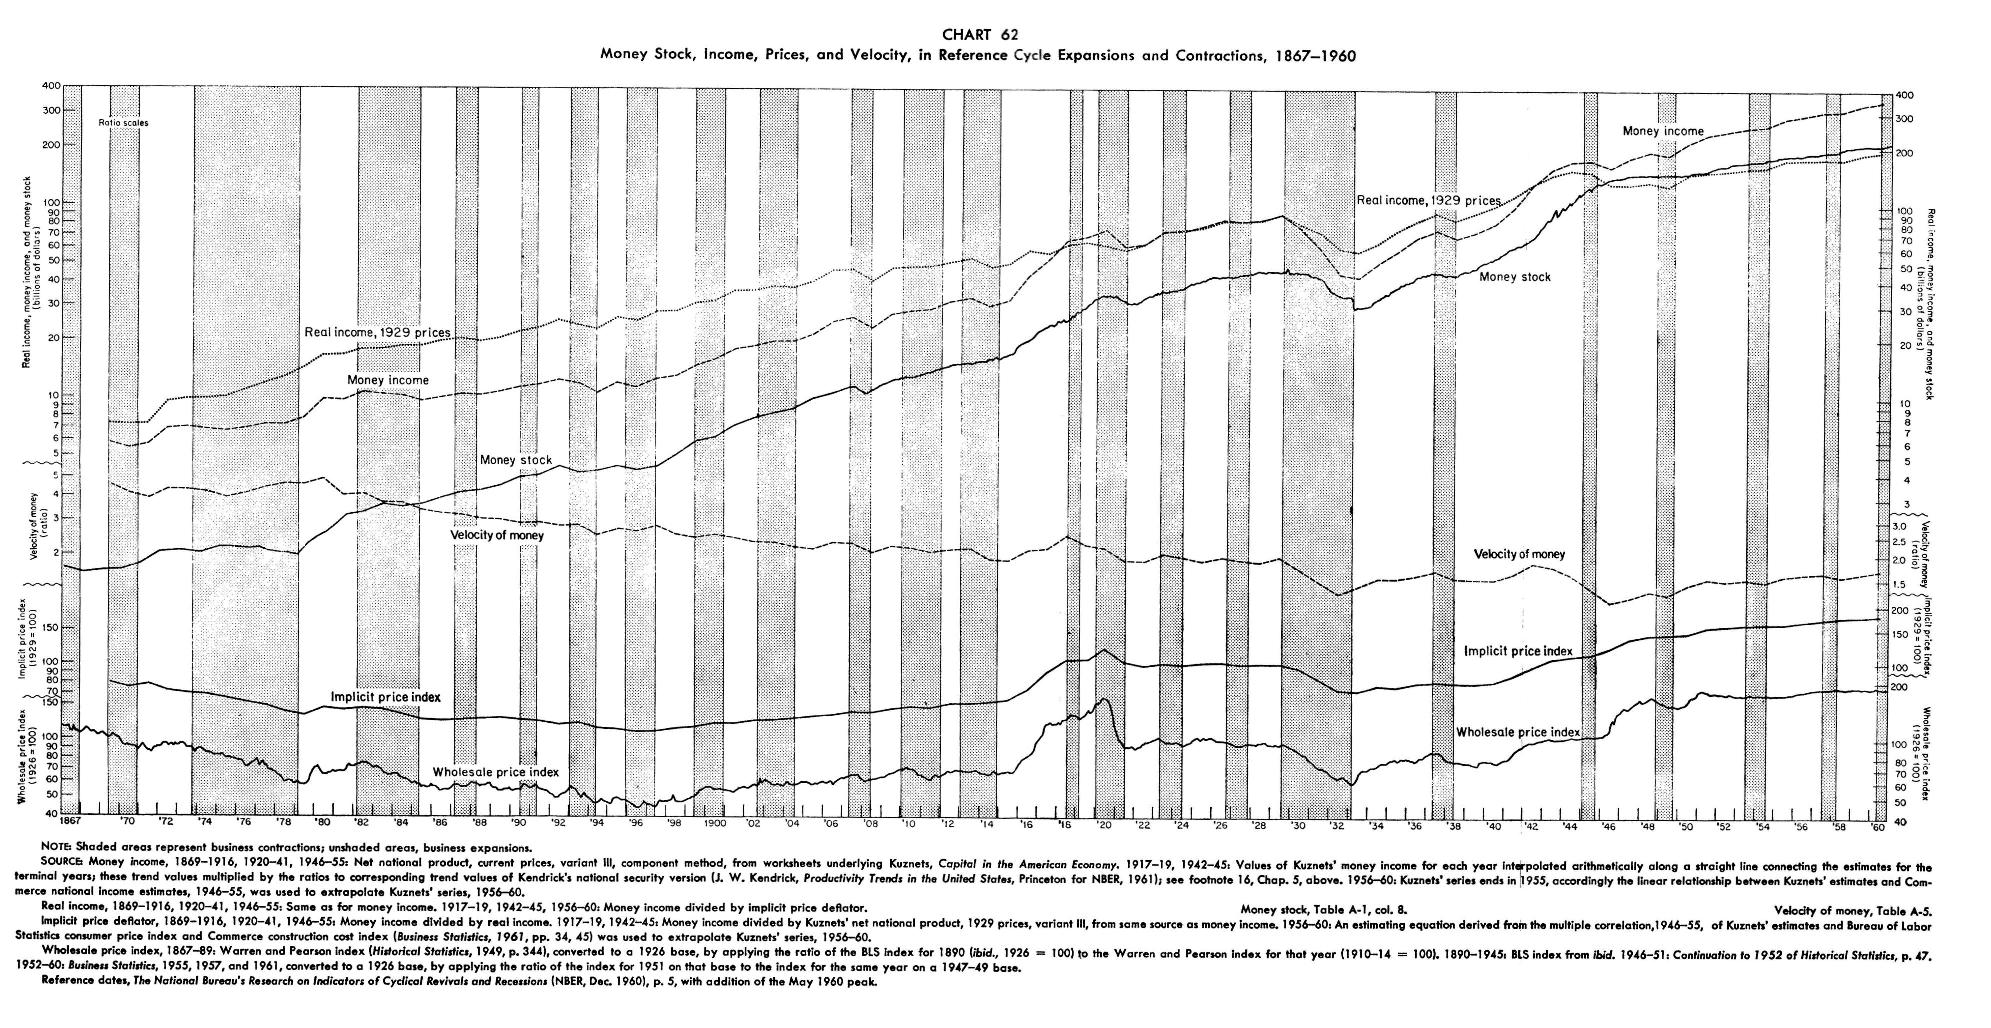
\includegraphics[width=1.0\textwidth]{4º Período/História do Pensamento Econômico/Tradução HPE/Tradução Tópico 9.1/Gráfico 62.png}
    \end{figure}
    
\subsubsection{\textbf{Estabilidade das Relações Monetárias}}

A relação entre dinheiro e outras variáveis econômicas não só tem sido próxima, mas também altamente estável em forma e caráter. Um exemplo marcante da estabilidade das relações econômicas básicas é o comportamento dos preços relativos nos Estados Unidos e na Grã-Bretanha, ajustados pelas mudanças na taxa de câmbio entre o dólar e a libra. Temos uma série razoavelmente contínua desde 1871 (Gráfico 63). Nos 79 anos de 1871 a 1949, ocorreram vastas mudanças na estrutura econômica e no desenvolvimento dos Estados Unidos, no papel da Grã-Bretanha na economia mundial, nas estruturas monetárias internas de ambos os países e nos arranjos monetários internacionais que os ligavam. No entanto, apesar dessas mudanças, apesar de duas guerras mundiais e apesar dos erros estatísticos nos números dos índices de preços, a razão de preço ajustada, expressa em uma base que faz 1929 = 100, esteve entre 84 e 111 em todos, exceto um dos 79 anos. A exceção foi 1932. Refletiu a desordem das relações monetárias internacionais que se seguiu à desvalorização da Grã-Bretanha no outono de 1931, que tornou a Grã-Bretanha temporariamente não representativa do mundo fora da área da libra com a qual os Estados Unidos negociavam. Dentro de um ano, a razão voltou ao intervalo anterior. Além disso, quase os extremos do intervalo foram experimentados na própria primeira década, durante a qual a razão variou de 111 em 1871 a 86 em 1876. Em 1950, depois que a Grã-Bretanha desvalorizou novamente no outono de 1949, a razão, como em 1932, disparou para fora do intervalo anterior, desta vez por uma quantidade muito mais significativa, para 143. Essa divergência durou mais tempo, em parte devido ao papel menor que a Grã-Bretanha passou a desempenhar na economia mundial, mas ainda mais, acreditamos, devido ao desenvolvimento de técnicas mais eficazes para suprimir a expressão de aumentos de preços ou seu equivalente em números de índices de preços computados. No entanto, ano a ano, a razão declinou até 1958, quando atingiu 118, apenas ligeiramente fora do intervalo anterior; e permaneceu aproximadamente nesse nível até 1960.

Mesmo que estejamos acostumados a considerar os Estados Unidos como quase autossuficientes, a integração econômica do mundo ocidental tem sido suficientemente próxima para deixar os preços dos EUA com pouca margem de manobra em relação aos preços externos, quando ambos são expressos em uma moeda comum. Houve mais flexibilidade em como a relação de preços foi alcançada — seja por meio de mudanças nos preços internos ou nas taxas de câmbio — do que na relação que poderia ser alcançada. Variações amplas em tarifas, um grande programa de compra de ouro, mudanças vastas na direção dos movimentos de capital (veja Gráfico 63) ou a imposição por nossos parceiros comerciais de controles extensivos de câmbio — nenhum desses fatores alterou radicalmente as relações de preços necessárias para produzir alguma medida de equilíbrio nos pagamentos internacionais.

\begin{figure}[H]
    \centering
    \caption{Gráfico 63}
    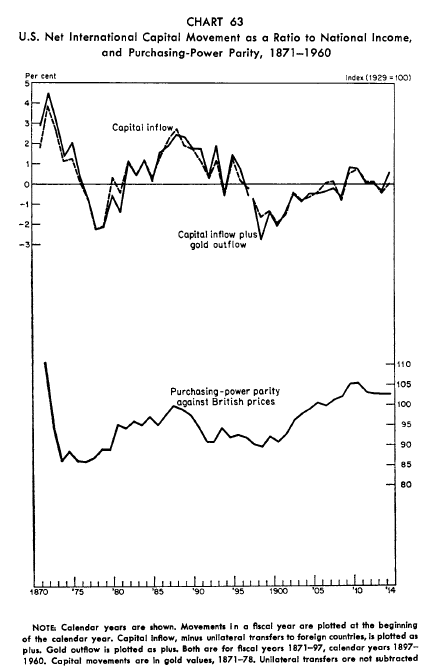
\includegraphics[width=1.0\textwidth]{4º Período/História do Pensamento Econômico/Tradução HPE/Tradução Tópico 9.1/Gráfico 63.png}
    \end{figure}

\begin{figure}[H]
    \centering
    \caption{Gráfico 63(Concluido)}
    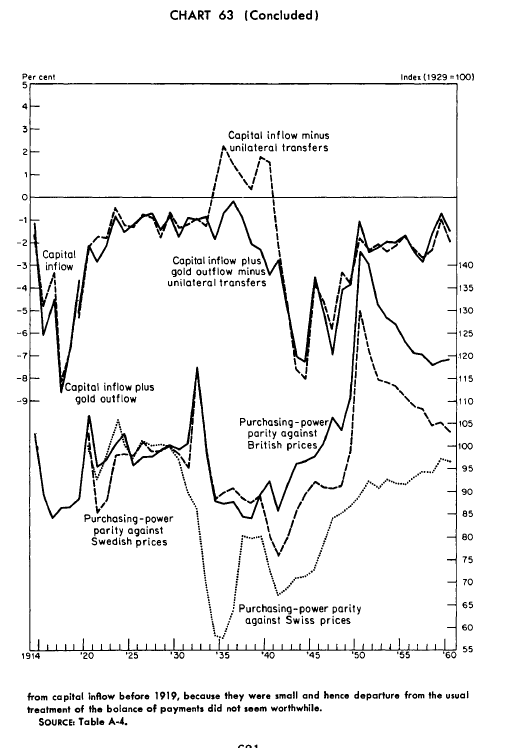
\includegraphics[width=1.0\textwidth]{4º Período/História do Pensamento Econômico/Tradução HPE/Tradução Tópico 9.1/Gráfico 63(Concluido).png}
    \end{figure}

A velocidade do dinheiro, que reflete as propensões de retenção de dinheiro da comunidade, oferece outro exemplo da estabilidade das relações monetárias básicas. À medida que a renda real da população dos Estados Unidos aumentava, e talvez também à medida que os depósitos se tornavam mais convenientes com a expansão das facilidades bancárias, a comunidade passou a reter uma quantidade consideravelmente maior de dinheiro em relação à sua renda, o que significa que a velocidade do dinheiro diminuiu. Em 1869, o estoque de dinheiro correspondia a menos de três meses de renda; em 1960, a mais de sete meses de renda. O valor numérico da velocidade, portanto, mudou consideravelmente. No entanto, a mudança ocorreu de forma bastante estável: um pouco mais rapidamente quando os preços estavam caindo durante a década de 1880 e início dos anos 1890, tornando a retenção de dinheiro mais atraente; e um pouco mais lentamente quando os preços estavam subindo de 1897 a 1914. As únicas grandes exceções foram durante e após a grande contração dos anos 1930, que viu uma grande queda na velocidade seguida de uma recuperação, e durante e após a Segunda Guerra Mundial, que também viu uma grande queda na velocidade seguida de uma recuperação pós-guerra. Em resposta às flutuações cíclicas, a velocidade mostrou um movimento sistemático e estável em torno de sua tendência, aumentando durante a expansão e diminuindo durante a contração. Mesmo o grande movimento que acompanhou a Grande Contração se encaixa parcialmente neste padrão; foi tão grande em parte porque o movimento cíclico foi muito grande.

Durante as nove décadas que terminaram em 1960, a velocidade do dinheiro caiu em média pouco mais de 1 por cento ao ano. Durante expansões econômicas, ela subiu ou caiu a uma taxa menor que essa; durante contrações, ela diminuiu a uma taxa maior que essa. As amplitudes do aumento e queda cíclicos tendiam a variar com a amplitude dos movimentos cíclicos na atividade econômica. Como muitos dos movimentos cíclicos na atividade econômica tinham aproximadamente a mesma amplitude, muitos dos movimentos cíclicos na velocidade também a tinham. Apesar da tendência secular, do padrão cíclico consistente e da margem de erro considerável em nossas estimativas, a mudança observada de ano para ano na velocidade foi inferior a 10 por cento em 78 das 91 mudanças de ano para ano de 1869, quando nossas figuras de velocidade começam, até 1960. Das 13 mudanças maiores, mais da metade ocorreu durante a Grande Contração ou as duas guerras mundiais, e a maior mudança foi de 17 por cento. Expressa como uma porcentagem de uma tendência secular, a velocidade estava dentro do intervalo de 90 a 110 em 53 anos, e de 85 a 115 em 66 anos. Dos 26 anos restantes, 12 foram durante os primeiros 15 anos, para os quais os números de renda são seriamente defeituosos, e 7 durante a Grande Contração e as duas guerras mundiais.

Outra relação monetária que tem sido altamente estável é a relação entre as mudanças no estoque de dinheiro e os movimentos cíclicos na atividade econômica. Em média, o estoque de dinheiro cresceu a uma taxa mais alta que a renda monetária; isso é o outro lado da queda secular na velocidade. O aumento foi mais rápido que o usual durante expansões cíclicas e menos rápido que o usual durante contrações cíclicas. A taxa de crescimento tendia a desacelerar bem antes do pico nos negócios e a acelerar bem antes do ponto mais baixo. Esse padrão prevalece durante todo o período, no ciclo mais antigo coberto por nossos dados e também no mais recente.

O leitor atento de nossa narrativa terá encontrado muitos outros exemplos detalhados de relações monetárias estáveis para complementar essas muito amplas: os efeitos semelhantes dos programas de compra de ouro empreendidos em 1878 para preparar a retomada e após 1933 para elevar os preços domésticos; a confiabilidade da razão depósito-moeda como um sinal de um problema de liquidez; os movimentos iniciais semelhantes dos preços no atacado dos EUA após o início das Guerras Mundiais I e II—em ambos os casos, em uma direção oposta à que prevaleceu mais tarde; e assim por diante.

Essas uniformidades persistiram apesar das mudanças radicais nos arranjos monetários. De 1862 a 1879, os Estados Unidos tinham uma moeda nacional independente, não conversível em ouro nem prata nem na moeda de nenhum outro país em qualquer proporção fixa. O estoque de dinheiro poderia, portanto, ser determinado internamente. De 1879 a 1914, o dinheiro dos EUA era conversível em ouro em uma proporção fixa especificada por lei e mantida na prática. O estoque de dinheiro e os preços internos tinham que estar em níveis que produzissem um equilíbrio aproximado nos pagamentos internacionais sem movimentos anormais de ouro. O estoque de dinheiro era uma variável dependente, não independente, embora, é claro, houvesse alguma margem de manobra em períodos curtos. Tanto antes quanto depois de 1879, até que o Sistema da Reserva fosse estabelecido, o sistema bancário unitário dos EUA era dividido entre bancos nacionais e não nacionais, cada um com cerca de metade dos depósitos totais, e nenhum sujeito a qualquer controle central exceto quando o Tesouro de tempos em tempos assumia funções de banco central.

De 1914 a 1933, o dinheiro dos EUA continuou a ser rigidamente vinculado ao ouro, mas o número de outras moedas nacionais assim vinculadas havia diminuído. Os Estados Unidos haviam alcançado um papel muito mais importante na economia mundial, e o comércio externo havia se tornado uma parte menor da atividade econômica dos EUA. Os vínculos entre o dinheiro dos EUA e o comércio internacional, portanto, eram muito mais frouxos do que nos anos anteriores. Além disso, o Federal Reserve Act não apenas estabeleceu controle central sobre a maior parte do sistema bancário, mas também forneceu uma agência que poderia intervir deliberadamente para alterar ou até reverter a relação entre os pagamentos internacionais e o estoque doméstico de dinheiro.

No início de 1933, o vínculo rígido entre o dinheiro dos EUA e o ouro foi rompido. Um ano depois, um vínculo rígido foi restabelecido em uma proporção diferente. No entanto, o padrão-ouro então restabelecido e legalmente vigente desde então era muito diferente do padrão pré-1933. O ouro foi eliminado da circulação, e a posse de ouro monetário por cidadãos privados foi tornada ilegal, de modo que o dinheiro nacional não era mais livremente conversível em ouro em uma proporção fixa. O afrouxamento dos vínculos entre o dinheiro e o ouro e, consequentemente, entre o dinheiro e o comércio internacional foi completado por outros países, muitos dos quais foram ainda mais longe ao cortar toda conexão entre o dinheiro nacional e o ouro. Hoje, o ouro é principalmente uma mercadoria cujo preço é fixado em vez de ser a pedra angular do sistema monetário mundial ou dos EUA. No entanto, o legado da história e o uso do ouro como veículo para fixação das taxas de câmbio ainda lhe conferem uma significância monetária que nenhuma outra mercadoria sujeita à fixação de preços pelo governo possui.

Uma grande mudança ocorreu no sistema bancário em 1934 como resultado do início do seguro federal de depósitos bancários. Parece ter tido sucesso, ao contrário do que ocorreu com o Federal Reserve Act, em tornar impossível a proliferação de uma perda de confiança pública em alguns bancos em um pânico bancário decorrente de uma tentativa generalizada por parte do público de converter depósitos em moeda.

Essas mudanças nos arranjos monetários alteraram significativamente as forças que determinam o estoque de dinheiro. Como resultado, elas também alteraram o comportamento do estoque de dinheiro. Por exemplo, nos 46 anos de 1914 a 1960, quando uma agência governamental tinha responsabilidade explícita pelo comportamento do estoque de dinheiro, a mudança de ano para ano no estoque foi uma magnitude mais variável do que nos 35 anos anteriores, quando era determinada pelo mecanismo quase automático do padrão-ouro. Por outro lado, no período desde o final da Segunda Guerra Mundial, tem sido uma magnitude muito menos variável do que em qualquer período anterior de comprimento comparável (Tabela 25).

As mudanças nos arranjos monetários afetaram de diversas maneiras as três variáveis que consideramos úteis para considerar como os determinantes aritméticos do estoque de dinheiro: o estoque de dinheiro de alta potência; a razão entre os depósitos do público e seus estoques de moeda; e a razão entre as obrigações de depósito do sistema bancário comercial e suas reservas, que definimos como igual aos seus totais de dinheiro de alta potência (Gráfico 64).

O estoque de dinheiro de alta potência foi o principal fator que contabilizou aritmeticamente as mudanças no estoque de dinheiro. As mudanças no dinheiro de alta potência, no entanto, foram produzidas por diferentes forças em diferentes momentos: no período dos "greenbacks", principalmente por mudanças nas emissões fiduciárias do governo; de 1879 a 1914, principalmente por fluxos de ouro, embora em alguma medida também por mudanças em notas bancárias nacionais e moeda emitida em troca de prata; de 1914 a 1960, principalmente por mudanças no crédito em circulação do Federal Reserve, com a notável exceção dos anos de 1934 a 1940, quando os fluxos de ouro dominaram.

\begin{figure}[H]
    \centering
    \caption{Gráfico 64}
    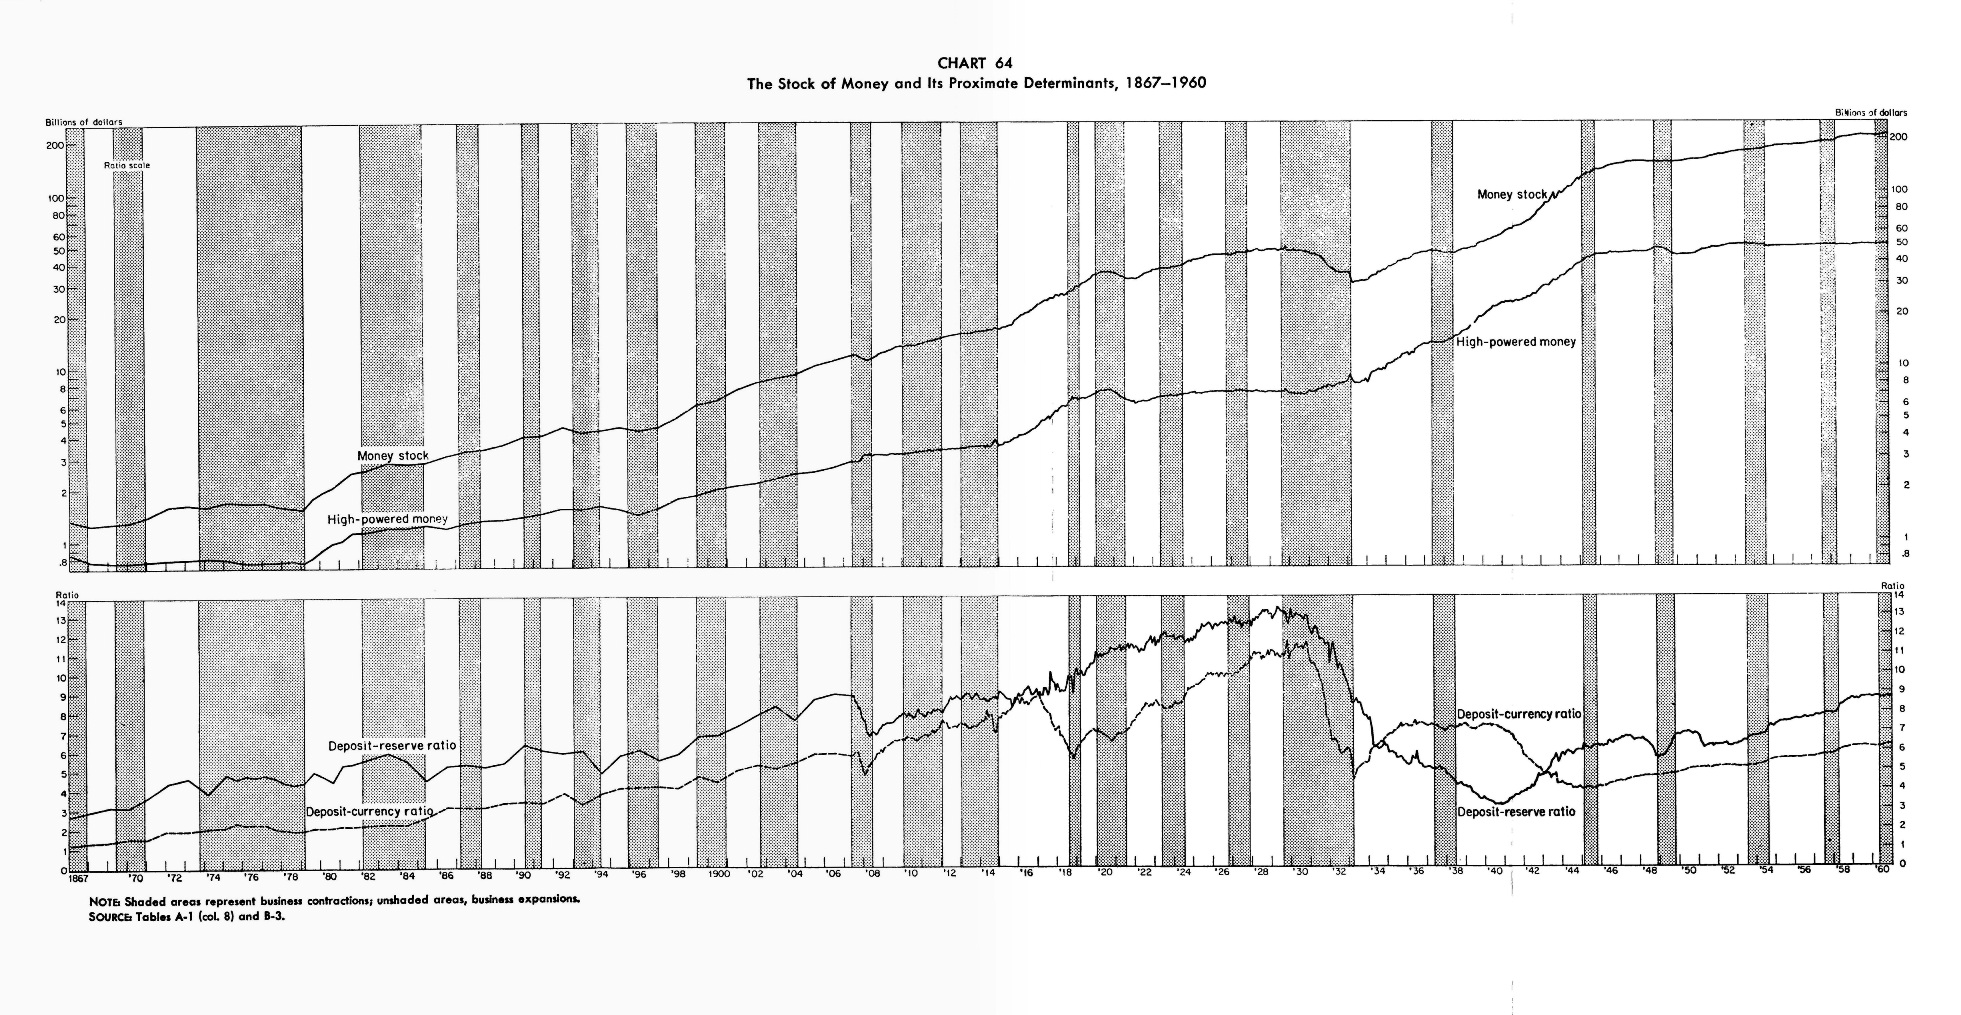
\includegraphics[width=1.0\textwidth]{4º Período/História do Pensamento Econômico/Tradução HPE/Tradução Tópico 9.1/Gráfico 64.png}
    \end{figure}

A relação depósito-moeda tem sido de grande importância principalmente durante períodos de dificuldades financeiras. Em cada um desses períodos, a perda de confiança do público nos bancos levou a uma tentativa de converter depósitos em moeda, o que resultou em uma forte queda na relação depósitos-moeda e uma forte pressão descendente sobre o estoque de dinheiro. Esperava-se que a criação do Sistema da Reserva Federal privasse tais mudanças na relação depósito-moeda de significância monetária, fornecendo um meio de aumentar o volume absoluto de moeda disponível para o público segurar, quando o público desejasse substituir depósitos por moeda, sem exigir uma contração múltipla dos depósitos. Na prática, isso não conseguiu alcançar esse objetivo. A mudança mais notável na relação depósito-moeda nos 93 anos de 1867 a 1960 ocorreu de 1930 a 1933, quando a relação caiu para menos da metade de seu valor inicial e, em três anos, apagou o aumento secular de três décadas. Embora o volume absoluto de moeda mantido pelo público tenha aumentado, isso ocorreu apenas à custa de uma queda muito maior nos depósitos, o efeito combinado sendo uma queda de um terço no estoque total de dinheiro. O início do seguro federal de depósitos bancários em 1934 finalmente mudou decisivamente o comportamento da relação depósito-moeda. Desde então, não tem sido sujeita a mudanças drásticas em curtos períodos, e é improvável que seja no futuro.

A relação depósitos-reservas, assim como a relação depósito-moeda, tem sido de grande importância em tempos de dificuldades financeiras, embora tenha desempenhado um papel mais consistente e menor, geralmente aumentando durante expansões empresariais e caindo durante contrações empresariais. Sempre que o público demonstrou desconfiança dos bancos ao procurar reduzir a relação depósito-moeda, os bancos reagiram procurando fortalecer suas reservas. Após um breve intervalo, eles conseguiram fazer isso, ou seja, baixando a relação depósito-reserva, adicionando assim mais pressão descendente sobre o estoque de dinheiro.

A relação depósito-reserva também variou ao longo de períodos mais longos em resposta a mudanças nos arranjos monetários. Aumentou notavelmente no período dos greenbacks como resultado da maturação dos bancos nacionais e um aumento na importância relativa dos bancos não nacionais. Aumentou novamente na década de 1897 a 1907, em parte como resultado da assunção pelo Tesouro de funções bancárias centrais mais amplas. Aumentou novamente após o estabelecimento do Sistema da Reserva Federal, que reduziu os requisitos legais e deu aos bancos a confiança de que, em caso de necessidade, eles tinham um "emprestador de última instância" para recorrer. O colapso monetário de 1930 a 1933 mudou profundamente o cenário. Produziu uma queda na relação depósito-reserva de seu ponto mais alto em 1929 para um nível, uma década depois, não muito acima do nível no início da nossa série em 1867. A experiência de 1930-33 ensinou aos bancos a não confiar no Sistema da Reserva Federal para liquidez; levou-os cerca de três anos para ajustar suas reservas à mudança associada em suas preferências por liquidez. Aumentos sucessivos nos requisitos de reservas em 1936-37 provocaram outra mudança em suas preferências; novamente, levou os bancos cerca de três anos para ajustar. Desde então, a relação depósito-reserva aumentou à medida que o papel do seguro de depósito em eliminar o perigo de corridas aos bancos foi reconhecido, e os efeitos das experiências anteriores desgastaram-se. Se for feito um ajuste para mudanças nos requisitos legais, a relação voltou ao seu nível do final dos anos vinte.

Apesar dessas alterações marcantes nas forças que afetam o estoque de dinheiro, houve, como vimos, pouca alteração na relação entre as mudanças, uma vez determinadas, no estoque de dinheiro e outras variáveis econômicas. As forças externas que

 incidem sobre o estoque de dinheiro mudaram radicalmente. Ao mesmo tempo, o impacto das mudanças no estoque de dinheiro no restante da economia parece ter sido altamente estável.

 \subsubsection{\textbf{Independência das Mudanças Monetárias}}

A estreita relação entre as mudanças no estoque de dinheiro e as mudanças em outras variáveis econômicas, por si só, não revela nada sobre a origem de qualquer uma delas ou a direção da influência. As mudanças monetárias podem estar dançando conforme a música tocada por mudanças que surgem independentemente em outras variáveis econômicas; as mudanças na renda e nos preços podem estar dançando conforme a música tocada por mudanças monetárias que surgem independentemente; as duas podem estar interagindo mutuamente, cada uma com alguns elementos de independência; ou ambas podem estar dançando conforme a música de um terceiro conjunto de influências. Um grande mérito do exame de uma ampla gama de evidências qualitativas, tão essencial em uma história monetária, é que ele fornece uma base para discriminar entre essas possíveis explicações da covariação estatística observada. Podemos ir além dos números por si só e, pelo menos em algumas ocasiões, discernir as circunstâncias antecedentes de onde surgiram os movimentos particulares que se tornam tão anônimos quando alimentamos as estatísticas no computador.

Uma coisa é abundantemente clara em nossa narrativa. As mudanças monetárias foram frequentemente independentes, no sentido de que muitas vezes não foram uma consequência imediata ou necessária de mudanças contemporâneas nas condições de negócios.

O exemplo mais claro é talvez a expansão monetária de 1897 a 1914, que foi mundial e refletiu um aumento na produção de ouro. O aumento na produção de ouro foi em parte uma consequência de décadas anteriores de preços em queda, o que incentivou a produção de ouro, e também fala por uma interação mútua entre mudanças monetárias e econômicas. Mas, claramente, a expansão monetária não pode ser atribuída ao aumento contemporâneo na renda monetária e nos preços. Por si só, o aumento na renda monetária e nos preços resultou em uma redução na produção de ouro no mundo e em um fluxo de ouro saindo de qualquer país em um mundo com padrão ouro. Se o movimento comum de dinheiro e renda não foi puramente coincidente, a direção da influência deve ser do dinheiro para a renda.

Os dois principais aumentos no estoque de dinheiro durante as Guerras Mundiais I e II são igualmente claros. Nos estágios iniciais de ambas as guerras, o aumento refletiu um influxo de ouro nos Estados Unidos, à medida que as nações beligerantes usavam os recursos que podiam mobilizar rapidamente para comprar material de guerra nos Estados Unidos. Os influxos de ouro não foram subprodutos de mudanças contemporâneas na atividade econômica neste país ou no exterior, como haviam sido nos anos antes de 1914. Eles foram uma consequência do início das duas guerras e das decisões políticas deliberadas das autoridades políticas nos países em guerra. Nos estágios posteriores de ambas as guerras, o aumento refletiu decisões políticas das autoridades dos EUA sobre o financiamento dos gastos com a guerra. Essas decisões envolveram uma expansão importante no dinheiro de alta potência, que continuou o trabalho iniciado pelos influxos de ouro. Novamente, se o movimento comum do estoque de dinheiro e da renda e preços monetários não é coincidente ou consequência de uma causa comum, a direção da influência deve ser do dinheiro para a renda.

Os episódios de retomada e prata mostram uma independência substancial nas mudanças monetárias que ocorreram e também uma ação e interação bastante complexas entre mudanças monetárias e de negócios. As pressões a favor e contra a retomada nos anos 1870 e a campanha pela prata gratuita nos anos 1890 foram elementos principais que moldaram o curso dos eventos. Ambos foram em alguma medida independentes do curso contemporâneo da atividade econômica, embora não, claro, dos desenvolvimentos econômicos de longo prazo. Ambos também foram muito afetados pelo curso dos eventos, as pressões contra a retomada e a favor da prata gratuita sendo muito fortalecidas por uma desaceleração ou declínio nos desenvolvimentos na indústria ferroviária nos anos 1870 e no mercado financeiro de Londres nos anos 1890 tiveram efeitos importantes nas datas específicas em que essas pressões políticas produziram distúrbios monetários, que por sua vez reagiram sobre as condições comerciais e as atitudes políticas.

A criação do Sistema da Reserva Federal oferece ao estudante de economia um substituto mais próximo do experimento controlado para determinar a direção da influência do que o cientista social geralmente pode obter. O Sistema foi, em alguns momentos, simplesmente um meio através do qual outras forças operavam — como durante as duas guerras mundiais e grande parte da década de 1930, quando seguiu um curso em grande parte passivo, e após a Segunda Guerra Mundial, quando sua política de sustentar os preços dos títulos governamentais deixou-lhe pouca iniciativa independente. No entanto, a criação do Sistema deu a um pequeno grupo de indivíduos o poder, que exerceram de tempos em tempos, de alterar o curso dos eventos de maneiras significativas e identificáveis através de um processo deliberativo — uma sequência paralela à condução de um experimento controlado. De fato, as ações das autoridades monetárias foram grandemente afetadas pelo clima de opinião e conhecimento no qual operavam. Suas atitudes, os experimentos que realizaram e a interpretação que deram aos resultados foram em grande medida determinados pelo curso contemporâneo dos eventos e pelo estado contemporâneo do conhecimento sobre fenômenos monetários. Isso também é verdade para os cientistas físicos ao decidir quais experimentos realizar e ao interpretar os resultados à luz de experimentos anteriores e do corpo contemporâneo de conhecimento. Em ambos os casos, tal dependência do estado existente de conhecimento não altera a independência científica dos eventos prévios ou contemporâneos das mudanças introduzidas nas variáveis controladas. O que isso significa em ambos os casos é simplesmente que estudantes posteriores podem reinterpretar os resultados dos experimentos à luz do corpo alterado de conhecimento e tirar conclusões diferentes das que foram tiradas pelos experimentadores originais.

De fato, também é frequentemente impossível e sempre difícil identificar com precisão os efeitos das ações das autoridades monetárias. Suas ações são tomadas em meio a muitas outras circunstâncias, e pode não ser claro se suas ações ou algumas das outras circunstâncias produziram os resultados observados. Isso é igualmente verdadeiro para os experimentos dos cientistas físicos. Nenhum experimento é completamente controlado, e a maioria dos experimentos adiciona pouco ao conhecimento testado e confirmado sobre o assunto do experimento. É o raro experimento crucial que lança uma enxurrada de luz sobre seu assunto — uma luz que nos cega para muitos experimentos menos importantes que foram necessários antes que o experimento crucial pudesse ser realizado.

Três contrapartes de tais experimentos cruciais se destacam no registro monetário desde a criação do Sistema da Reserva Federal. Em três ocasiões, o Sistema tomou deliberadamente medidas políticas de grande magnitude que não podem ser consideradas consequências econômicas necessárias ou inevitáveis das mudanças contemporâneas na renda monetária e preços. Como os experimentos cruciais do cientista físico, os resultados são tão consistentes e claros que deixam pouca dúvida sobre sua interpretação. As datas são janeiro-junho de 1920, outubro de 1931 e julho de 1936-janeiro de 1937. Estas são as três ocasiões — e as únicas três — quando o Sistema da Reserva interveio de forma acentuadamente restritiva: em janeiro de 1920, elevando a taxa de redesc
onto de 4\% para 6\% e, em junho de 1920, para 7\%, em um momento em que os bancos membros estavam tomando emprestado dos Bancos da Reserva mais do que o total de seus saldos de reserva; em outubro de 1931, elevando a taxa de redesconto de 1,5\% para 3,5\% em um período de duas semanas, em um momento em que uma onda de falências estava engolindo bancos comerciais, como no ano anterior, e a dívida com o Sistema estava crescendo; em julho de 1936 e janeiro de 1937, anunciando a duplicação dos requisitos de reserva em três etapas, sendo a última efetiva em 1º de maio de 1937, em um momento em que o Tesouro estava engajado na esterilização de ouro, o que equivalia a uma operação restritiva de mercado aberto em grande escala. Não há outra ocasião na história do Federal Reserve em que tenha tomado medidas restritivas explícitas de magnitude comparável — não podemos nem sugerir possíveis paralelos.

As mudanças estritamente monetárias associadas a essas ações foram igualmente marcantes e distintas. As ações foram seguidas, após alguns meses em 1920 e 1936-37, e imediatamente em 1931, por quedas acentuadas no estoque de dinheiro, as três maiores quedas dentro de um período de doze meses na história do Sistema da Reserva: quedas de 9\% (1920), 14\% (1931) e 3\% (1937), respectivamente. E para as duas primeiras quedas, os números subestimam a severidade da reação monetária. Em 1919 e novamente em 1936, o estoque de dinheiro estava crescendo a uma taxa rápida, então os declínios subsequentes representaram uma desaceleração de uma taxa de crescimento incomumente alta para uma taxa de declínio igualmente alta. O declínio de 1931 — o declínio absoluto mais severo dos três — foi o mais brando em termos de desaceleração; o estoque de dinheiro no ano anterior estava caindo a uma taxa ligeiramente menor, então o aumento na taxa de declínio no ano que começou em outubro de 1931 foi de apenas cerca de um ponto percentual.

As mudanças econômicas associadas a essas ações monetárias foram igualmente marcantes e distintas. Cada uma foi seguida por contrações acentuadas na produção industrial, após alguns meses em 1920 e 1936-37, e imediatamente em 1931: declínios dentro de um período de doze meses de 30\% (1920), 24\% (1931) e 34\% (1937), respectivamente. Há apenas duas outras quedas comparativamente severas na produção industrial: durante 1929-31, que será abordado mais adiante; e 1945, quando a queda acentuada representou uma mudança na composição da produção, afastando-se dos produtos militares após o fim da guerra, em vez de uma contração geral na atividade econômica, como nas outras quatro datas. Outros indicadores confirmam a história contada pela produção industrial. Seja olhando para os preços no atacado, carregamentos de vagões de carga, preços de ações comuns ou vendas em lojas de departamento, as quedas que seguiram as três ações monetárias são as mais severas, por uma ampla margem, na história do Sistema da Reserva Federal, exceto apenas a queda de 1929 a 1931.

A força das evidências fornecidas por esses três experimentos quase controlados pode talvez ser esclarecida por uma analogia. Suponha que temos registros médicos de 42 casais casados (para corresponder aos 42 anos de história do Federal Reserve de 1919 a 1960, excluindo a Primeira Guerra Mundial porque o Sistema não estava efetivamente no controle). Suponha que 3 homens e 4 mulheres foram encontrados com uma doença especificada; suponha que 3 das 4 mulheres acabaram sendo esposas dos 3 homens com a mesma doença. A presunção de que a doença era contagiosa certamente seria muito forte — especialmente se fosse descoberto que o marido da quarta mulher era o único homem restante a ter uma doença biologicamente relacionada, mas não idêntica. Da mesma forma, os três episódios descritos acima estabelecem uma presunção comparativamente forte de que as mudanças econômicas foram consequência das ações monetárias deliberadamente empreendidas e, portanto, que nossa descoberta de uma covariação próxima entre o estoque de dinheiro e a renda reflete a existência de uma influência do dinheiro para a renda. De fato, em um aspecto, a analogia subestima seriamente a força das evidências. Ela não leva em conta a sequência temporal dos eventos.

A presunção de que as mudanças econômicas foram consequência das mudanças monetárias é bastante reforçada pelo exame da única contração econômica acentuada não associada a medidas restritivas explícitas do Sistema da Reserva Federal - a contração de 1929 a 1931, que foi a primeira parte da grande contração de 1929 a 1933. Essa contração serviu, talvez mais do que qualquer outra experiência, para fortalecer a visão de que o dinheiro dança conforme a música dos negócios. A razão é que o Sistema da Reserva não conseguiu, de fato, deter a queda de um terço no estoque de dinheiro - de longe a maior no curso de uma contração cíclica pelo menos desde 1893-43 - ou a contração econômica acompanhante. O Sistema alegou impotência, argumentando explicitamente que as forças não monetárias que induziam a contração eram tão fortes e violentas que estava impotente para deter a maré, e implicitamente que a profundidade da queda no estoque de dinheiro se devia à profundidade da queda na atividade empresarial, em vez de, como as evidências citadas acima sugerem, o inverso. Muitos outros, reconhecendo as boas intenções das autoridades monetárias e a capacidade de muitos indivíduos no Sistema, enquanto mantinham uma variedade de visões sobre o papel do dinheiro nos assuntos econômicos, aceitaram a alegação do Sistema. Além disso, uma revolução na teoria econômica, com origens bastante diferentes e de forma alguma necessariamente implicando a impotência da política monetária, ofereceu uma estrutura teórica que ao mesmo tempo poderia racionalizar a impotência da política monetária e fornecer uma explicação alternativa intelectualmente satisfatória para o desastre econômico.

Há um sentido - e, pelo que podemos ver, apenas um - em que se pode argumentar que o declínio monetário foi uma consequência do declínio econômico. Esse sentido não é relevante para nossa principal tarefa de buscar entender as inter-relações econômicas, pois envolve confiar principalmente em fatores psicológicos e políticos. O Sistema operava em um clima de opinião que, em geral, considerava as recessões e depressões como episódios curativos, necessários para purgar a economia dos efeitos posteriores de seus excessos anteriores. A opinião predominante também confundia dinheiro e crédito; confundia a elasticidade de um componente do estoque de dinheiro em relação a outro com a elasticidade do estoque total; considerava desejável que o estoque de dinheiro respondesse às "necessidades do comércio", aumentando nas expansões e diminuindo nas contrações; e atribuía muito mais importância à manutenção do padrão-ouro e à estabilidade das trocas do que à manutenção da estabilidade interna. A maioria dessas atitudes caracterizava o público em geral e não apenas a comunidade financeira ou o Sistema da Reserva em particular. Dado esse contexto, pode-se argumentar que o Sistema seguiu uma política inevitável; que não se poderia esperar que ele evitasse o declínio considerável no estoque de dinheiro durante 1930, porque ele e outros também consideravam o declínio um compensador desejável para excessos especulativos anteriores; e que sua falha em reagir vigorosamente, depois que os bancos começaram a falir em grande escala no final de 1930 e o público procurou converter depósitos em moeda, refletia a atitude de que era desejável liquidar os "maus" bancos, deixar a "natureza seguir seu curso" em vez de apoiar o sistema financeiro "artificialmente". Certamente, a prioridade dada à manutenção do padrão-ouro foi, em um sentido imediato, a razão para a forte elevação nas taxas de desconto em outubro de 1931, após a saída da Grã-Bretanha do ouro e um fluxo de saída de ouro dos Estados Unidos - a ação restritiva descrita acima como um dos experimentos cruciais do Sistema.

Esta conta retrata com precisão uma parte importante da situação. Ela ajuda a explicar como homens capazes e de espírito público poderiam ter agido de uma maneira que, em retrospectiva, parece equivocada, por que havia uma ausência tão notável de estadistas econômicos fora do Sistema e, portanto, nenhuma pressão informada constante no Sistema para uma ação diferente. Mas mesmo nesse nível, a conta está seriamente incompleta. Estamos inclinados a acreditar que o curso particular de ação seguido pelo Sistema de Reserva deveu menos ao clima de opinião - embora certamente fosse uma condição necessária - do que a uma sequência de eventos mais ou menos acidentais e ao conflito em curso pelo poder dentro do Sistema. A morte de Benjamin Strong em 1928 desencadeou uma fase ativa de conflito que dominou a política durante todo o ano de 1929, produzindo um impasse entre o Conselho e o Banco de Nova York - atuando como líder de todos os Bancos - sobre a política adequada a adotar diante do boom do mercado de ações. O resultado foi uma política que, em nossa opinião, era muito fácil para quebrar o mercado de alta e muito apertada para permitir uma expansão vigorosa dos negócios. O conflito, somado à reação do restante do Sistema às operações independentes (e eficazes) do Banco de Nova York na esteira do crash do mercado de ações em outubro de 1929, levou indiretamente a uma mudança de poder sobre as operações de mercado aberto. Um comitê de 5 homens, dominado pelo Banco de Nova York, foi substituído por um comitê de 12 homens dos 12 governadores do Federal Reserve Bank, no qual Nova York desempenhou um papel menos importante. Essa mudança empilhou fortemente as cartas a favor de uma política de inação e deriva.

Compartilhamos a visão expressa por Carl Snyder, por muitos anos associado ao Banco de Nova York como estatístico e economista, de que se Benjamin Strong pudesse "ter tido mais doze meses de saúde vigorosa, poderíamos ter encerrado a depressão em 1930, e com isso a longa crise mundial que afetou tão profundamente os desenvolvimentos políticos subsequentes."3 Como estava, o sucessor de Strong em Nova York, George L. Harrison, defendeu vigorosamente a ação expansionista em 1930, mas não conseguiu prevalecer sobre a oposição combinada do Conselho e dos outros governadores do Banco. Harrison era a favor de ação expansionista em 1931, dessa vez com o apoio do novo governador do Conselho, Eugene Meyer, mas o padrão de impasse e inação havia sido estabelecido, para ser quebrado apenas temporariamente em 1932 sob a pressão do Congresso. Apesar do clima geral de opinião, o pessoal técnico do Banco de Nova York - e deve-se lembrar que sob Strong o Banco de Nova York dominava quase completamente a política do Sistema - era consistentemente a favor das políticas que nos parecem em retrospectiva as que deveriam ter sido seguidas.

De qualquer forma, o que é relevante para o nosso propósito atual não é nem elogio nem culpa, nem mesmo uma compreensão completa das razões para o comportamento do Sistema sob as circunstâncias difíceis e desafiadoras que enfrentou. Mesmo que seu comportamento fosse psicologicamente ou politicamente inevitável sob as circunstâncias, isso explicaria apenas por que o experimento quase controlado foi conduzido. Não explicaria os resultados do experimento. A questão permaneceria se as mudanças monetárias eram o resultado inevitável das mudanças econômicas, de modo que, se o Sistema não tivesse sido o intermediário, algum outro mecanismo teria imposto as mesmas mudanças monetárias; ou se as mudanças monetárias podem ser consideradas um fator economicamente independente que contabilizou em grande medida as mudanças econômicas. Há pouca dúvida sobre a resposta. Em todos os momentos durante a contração de 1929-33, políticas alternativas estavam disponíveis para o Sistema pelo qual ele poderia ter mantido o estoque de dinheiro de cair, e de fato poderia ter aumentado a quase qualquer taxa desejada. Essas políticas não envolviam inovações radicais. Eles envolviam medidas do tipo que o Sistema havia tomado em anos anteriores, do tipo explicitamente contemplado pelos fundadores do Sistema para atender precisamente o tipo de crise bancária que se desenvolveu no final de 1930 e persistiu depois disso. Eles envolveram medidas que foram realmente propostas e muito provavelmente teriam sido adotadas sob uma estrutura burocrática ou distribuição de poder ligeiramente diferente, ou mesmo se os homens no poder tivessem personalidades um pouco diferentes. Até o final de 1931 - e acreditamos que nem mesmo então - as políticas alternativas não envolviam conflito com a manutenção do padrão-ouro. Até setembro de 1931, o problema que recorrentemente perturbava o Sistema era como manter os influxos de ouro sob controle, não o contrário.

Para considerar ainda outra alternativa: se o sistema bancário pré-1914, em vez do Sistema Federal de Reserva, estivesse em existência em 1929, o estoque de dinheiro quase certamente não teria sofrido um declínio comparável ao que ocorreu. A comparação do pânico bancário de 1907 sob o sistema anterior e a crise de liquidez muito semelhante que começou no final de 1930 oferece fortes evidências para este julgamento. Se o sistema anterior estivesse em operação, e se tudo o mais tivesse procedido como fez até dezembro de 1930, a experiência de 1907 sugere fortemente que haveria uma reação inicial mais severa às falências bancárias do que houve em 1930, provavelmente envolvendo restrição concertada pelos bancos da conversibilidade de depósitos em moeda. A restrição pode ter tido efeitos iniciais mais severos para aprofundar a contração econômica do que a pressão persistente sobre o sistema bancário que caracterizou o final de 1930 e o início de 1931 teve. Mas também teria interrompido a propagação da crise, teria impedido a acumulação de falências bancárias e teria tornado possível, como fez em 1908, a recuperação econômica após alguns meses.

Portanto, enquanto as ações do Sistema de Reserva em 1929-33 podem ser compreensíveis sob as circunstâncias, mesmo psicologicamente e politicamente inevitáveis, a contração é uma evidência adicional forte para a independência econômica das mudanças monetárias em relação ao curso contemporâneo de renda e preços, mesmo durante a fase inicial da contração, de 1929 a 1931, quando o declínio no estoque de dinheiro não foi o resultado de medidas restritivas explícitas tomadas pelo Sistema. Pode de fato ser considerado como um quarto experimento crucial, fazendo a correspondência de declínio monetário independente e subsequente declínio econômico 4 para 4.

A existência de uma influência independente importante que vai do dinheiro para a renda explica o contraste que notamos entre a variabilidade nos arranjos monetários durante o quase século que estudamos e a estabilidade da relação entre as mudanças no dinheiro e em outras variáveis econômicas. A variabilidade dos arranjos monetários produziu, como vimos, uma variação correspondente nos movimentos do próprio dinheiro. Mas, dado que o principal canal de influência é do dinheiro para os negócios, não há razão para que as mudanças nos arranjos monetários tenham alterado a relação entre os movimentos do dinheiro e dos negócios. Essa relação é determinada principalmente pelos canais através dos quais o dinheiro afeta os negócios. Enquanto eles permanecerem os mesmos, como aparentemente têm, também deve ser a relação entre dinheiro e negócios.

Suponha, no entanto, que o principal canal de influência tenha sido dos negócios para o dinheiro. Mudanças nas instituições monetárias então teriam afetado não apenas o comportamento do dinheiro, mas também a relação entre o dinheiro e outras variáveis econômicas, uma vez que uma mudança nos negócios teria tido efeitos diferentes no estoque de dinheiro sob os diferentes arranjos monetários. Sob o padrão-ouro pré-1914, por exemplo, uma expansão dos negócios nos Estados Unidos tendia a gerar um déficit na balança de pagamentos, que por sua vez tendia a produzir uma saída de ouro e, portanto, pressão descendente sobre o estoque de dinheiro. Esse elo particular na sequência foi em grande parte rompido pela política de esterilização do ouro seguida pelo Federal Reserve na década de 1920 e pelo Tesouro em parte da década de 1930, e foi bastante enfraquecido pela mudança no caráter do padrão-ouro durante o restante do período após 1914. Tanto antes quanto depois de 1914, a expansão dos negócios elevou as taxas de juros e estimulou os bancos a se expandirem. No entanto, antes de 1914, um aumento nas taxas de juros poderia aumentar o estoque de dinheiro apenas através de um aumento na relação depósito-reserva ou através da atração de capital e, portanto, ouro do exterior. Após 1914, um aumento nas taxas de juros também poderia aumentar o estoque de dinheiro, induzindo os bancos a pedirem empréstimos mais pesados do Sistema de Reserva Federal. Se a direção predominante da influência tivesse sido dos negócios para o dinheiro, essas e outras mudanças nos elos entre negócios e dinheiro provavelmente teriam produzido uma relação apreciavelmente diferente entre os movimentos dos dois antes e depois de 1914, e talvez também para subdivisões adicionais desses períodos.

Embora a influência que vai do dinheiro para a atividade econômica tenha sido predominante, também houve claramente influências no sentido contrário, particularmente durante os movimentos de curto prazo associados ao ciclo de negócios. O padrão cíclico da relação depósito-reserva é um exemplo. A retomada e os episódios de prata, a inflação de 1919 e a contração de 1929-33 revelam claramente outros aspectos da influência reflexa dos negócios sobre o dinheiro. As mudanças no estoque de dinheiro são, portanto, uma consequência, bem como uma fonte independente de mudança na renda monetária e nos preços, embora, uma vez que ocorram, produzam por sua vez ainda mais efeitos sobre a renda e os preços. Interação mútua, mas com o dinheiro sendo claramente o parceiro sênior em movimentos de longo prazo e em movimentos cíclicos maiores, e mais quase um parceiro igual com a renda monetária e os preços em movimentos mais curtos e mais suaves - esta é a generalização sugerida por nossa evidência.

\subsubsection{\textbf{Enganos das Aparências}}
O dinheiro é um assunto fascinante de estudo porque está cheio de mistério e paradoxo. O pedaço de papel verde com impressão nele é pouco diferente, como papel, de um pedaço do mesmo tamanho rasgado de um jornal ou revista, no entanto, o primeiro permitirá ao seu portador comandar uma certa medida de comida, bebida, roupa e os demais bens da vida; o outro serve apenas para acender o fogo. De onde vem a diferença? O pedaço de papel verde lê, "Os Estados Unidos da América pagarão ao portador sob demanda... dólares", ou palavras nesse sentido, além de uma afirmação de que é "moeda legal". Mas, nas circunstâncias atuais, a promessa equivale apenas a um compromisso de trocar um pedaço de papel verde por um ou vários outros pedaços de papel verde ou por moedas que, se derretidas, venderão no mercado como metal por menos do que a quantidade de dinheiro em papel que servem para resgatar. A qualidade de moeda legal significa apenas que o governo aceitará os pedaços de papel para quitar dívidas devidas a si mesmo, e que os tribunais os considerarão como quitando dívidas expressas em dólares. Por que eles também deveriam ser aceitos por pessoas privadas em transações privadas por bens e serviços?

A resposta curta - mas a resposta correta - é que cada um os aceita porque tem confiança de que os outros também o farão. Os pedaços de papel verde têm valor porque todo mundo acha que eles têm valor, e todo mundo acha que eles têm valor porque em sua experiência eles tiveram valor. Nossa economia não poderia operar em mais do que uma pequena fração de seu atual nível de produtividade sem um meio comum e amplamente aceito de troca; ainda assim, esse meio comum e amplamente aceito de troca é, em última análise, uma convenção social que deve sua própria existência à aceitação mútua do que, de um ponto de vista, é uma ficção.

A convenção social ou a ficção ou o que você quiser não é uma coisa frágil. Pelo contrário, o valor social de um dinheiro comum é tão grande que as pessoas se apegarão à ficção mesmo sob extrema provocação - daí, é claro, vem parte dos ganhos que podem ser obtidos com a inflação pelos emissores do dinheiro e, portanto, também a tentação de inflar. Mas nem a ficção é indestrutível: variação extrema na quantidade do papel verde - como na Guerra Revolucionária dos EUA ou nas hiperinflações em vários países após as Guerras Mundiais I e II - ou variação moderada em sua quantidade mais tetos legalmente e efetivamente aplicados sobre preços nominais - como na Alemanha após a Segunda Guerra Mundial - podem tornar o papel que antes servia como dinheiro sem valor e induzir as pessoas a procurar substitutos - como os cigarros e conhaque que por um tempo se tornaram o meio de troca na Alemanha após a Segunda Guerra Mundial.

O dinheiro é um véu. As "verdadeiras" forças são as capacidades das pessoas, sua indústria e engenhosidade, os recursos que comandam, seu modo de organização econômica e política, e coisas do tipo. Como John Stuart Mill escreveu há mais de um século:

Não pode haver, em suma, intrinsecamente uma coisa mais insignificante, na economia da sociedade, do que o dinheiro; exceto no caráter de um artifício para poupar tempo e trabalho. É uma máquina para fazer rapidamente e comodamente, o que seria feito, embora menos rapidamente e comodamente, sem ela: e como muitos outros tipos de maquinário, só exerce uma influência distinta e independente de si mesma quando sai de ordem.

Perfeitamente verdadeiro. No entanto, também um tanto enganoso, a menos que reconheçamos que dificilmente há um artifício que o homem possui que pode causar mais danos a uma sociedade quando dá errado.

Cada homem acredita que pode determinar quanto de sua riqueza ele manterá em dinheiro; no entanto, a quantidade total de dinheiro disponível para todos segurarem está fora do controle de todos os detentores de dinheiro juntos. Cada banco acredita que pode determinar quanto de seus ativos manterá na forma de moeda, mais depósitos nos Bancos da Reserva Federal, para atender aos requisitos de reserva legal e para fins de precaução. No entanto, a quantidade total disponível para todos os bancos segurarem está fora do controle de todos os bancos juntos. Se qualquer banco recebe um acréscimo ao seu dinheiro, pode adquirir ativos não monetários adicionais iguais no máximo a esse acréscimo; no entanto, se todos os bancos juntos receberem um acréscimo de dinheiro, o sistema bancário pode adquirir ativos adicionais iguais a um múltiplo desse acréscimo.

Essa enganosidade das aparências ocorreu repetidamente no curso de nossa narrativa. O preço do ouro em termos de notas verdes durante a Guerra Civil pode ter flutuado de dia para dia de acordo com as mudanças nas fortunas da guerra; mas as fortunas da guerra afetaram apenas em menor medida o nível em torno do qual as flutuações ocorreram - apenas na medida em que afetaram a disposição dos estrangeiros em manter notas verdes ou títulos expressos em termos de notas verdes. O nível refletia, ao invés disso, o declínio drástico nas exportações de algodão e os preços internos crescentes no Norte à medida que o dinheiro era emitido para ajudar a financiar a guerra.
Uma medida tomada para promover a retomada, ou seja, para aumentar o valor do dólar em termos de moedas estrangeiras, era idêntica a uma medida tomada por Franklin D. Roosevelt para alcançar exatamente o propósito oposto, para diminuir o valor do dólar em termos de moeda estrangeira. Em ambos os casos, o Tesouro se comprometeu a comprar ouro no exterior.
A economia do New Deal estava correta, pelo menos neste aspecto; portanto, a adoção da mesma medida durante o período das notas verdes significava que os efeitos mecânicos da compra de ouro no exterior tornavam a retomada mais difícil do que menos difícil.

Embora a retomada tenha sido uma questão política importante por uma década e meia, seu sucesso deveu pouco às medidas tomadas em seu nome. A principal contribuição governamental foi uma redução menor no dinheiro de alta potência - concedido, não é uma conquista insignificante em um nível puramente político, tendo em vista a pressão para expandir a emissão de notas verdes. A retomada teve sucesso porque o rápido crescimento da produção trouxe uma redução pela metade do nível de preços, apesar de um leve aumento no estoque de dinheiro. As medidas governamentais que tiveram o maior efeito na retomada não foram as medidas monetárias explicitamente, mas os atos de omissão e comissão que contribuíram para o rápido crescimento da produção.

Os defensores da prata livre foram atacados pelas forças do "dinheiro sólido" com o argumento de que a prata livre produziria uma expansão indevidamente rápida no estoque de dinheiro e, assim, geraria inflação de preços. As compras limitadas de prata feitas pelo Tesouro foram lamentadas porque se acreditava que aumentavam indevidamente o estoque de dinheiro e, portanto, eram precursores da inflação que seria desencadeada por compras ilimitadas. Na verdade, dado que o padrão-ouro não foi abandonado, o principal dano econômico causado pela agitação da prata foi que impôs uma taxa de aumento indevidamente lenta no estoque de dinheiro e, assim, produziu deflação. Fez isso porque o medo de que os Estados Unidos abandonassem o ouro reduziu os influxos de capital que de outra forma teriam sido maiores, ou fomentou fugas de capital. Por sua vez, esses exigiram preços mais baixos nos Estados Unidos do que de outra forma teriam sido necessários para equilibrar os pagamentos internacionais nas taxas de câmbio fixadas pelos preços oficiais do ouro nos Estados Unidos e no exterior.

A derrota de Bryan em 1896 marcou o auge da agitação da prata. Foi o auge, não porque Bryan perdeu sua língua de prata, nem porque os defensores do "dinheiro sólido" persuadiram os defensores da prata livre com seus argumentos, mas porque as descobertas de ouro e melhorias na mineração e refino de ouro fizeram do ouro o veículo efetivo para a inflação que Bryan e seus seguidores buscavam alcançar com a prata.

O pânico bancário de 1907 produziu uma pressão aparentemente irresistível para a reforma bancária. No entanto, encontramos razões para acreditar que pelo menos a etapa final desse pânico, a restrição concertada pelos bancos da conversibilidade de depósitos em moeda, foi uma medida terapêutica que interrompeu a crise de liquidez, impediu que bons bancos falissem em massa como vítimas de histeria coletiva e, ao custo de dificuldades severas, mas breves, possibilitou a recuperação e expansão após uma contração de curta duração.

A medida de reforma finalmente promulgada - o Sistema de Reserva Federal - com o objetivo de prevenir quaisquer pânicos ou qualquer restrição de convertibilidade no futuro, na verdade não conseguiu conter o pior pânico da história econômica americana e as restrições mais severas de convertibilidade, o colapso do sistema bancário de 1930 a 1933, terminando no feriado bancário de março de 1933. Essa mesma reforma, destinada a promover a estabilidade monetária, foi seguida por cerca de trinta anos de instabilidade relativamente maior no estoque de dinheiro do que qualquer experiência no período pré-Reserva Federal que nossos dados cobrem, e possivelmente do que qualquer experiência em toda a história dos EUA, exceto a Guerra Revolucionária.

O boom do mercado de ações e o rescaldo da preocupação com a inflação da Primeira Guerra Mundial levaram a uma crença generalizada de que a década de 1920 foi um período de inflação e que o colapso de 1929 a 1933 foi uma reação a isso. Na verdade, a década de 1920 foi, se alguma coisa, um período de deflação relativa: de 1923 a 1929 - para comparar os anos de pico dos ciclos de negócios e assim evitar distorções das influências cíclicas - os preços no atacado caíram à taxa de 1 por cento ao ano e o estoque de dinheiro subiu à taxa anual de 4 por cento ao ano, que é aproximadamente a taxa necessária para acompanhar a expansão da produção. A expansão do ciclo de negócios de 1927 a 1929 foi a primeira desde 1891-93 durante a qual os preços no atacado caíram, mesmo que apenas um pouco, e não houve nenhuma desde então.

O colapso monetário de 1929 a 1933 não foi uma consequência inevitável do que havia acontecido antes. Foi um resultado das políticas seguidas durante aqueles anos. Como já observado, políticas alternativas que poderiam ter interrompido a debacle monetária estavam disponíveis durante todos esses anos. Embora o Sistema de Reserva proclamasse que estava seguindo uma política de dinheiro fácil, na verdade seguiu uma política extremamente restritiva.

Os defensores do New Deal eram fortemente a favor do dinheiro fácil. E houve uma rápida expansão monetária durante os anos trinta, produzida principalmente por duas coisas: a alta no preço do ouro e a ascensão de Hitler ao poder, que estimulou um fluxo de capital para os Estados Unidos. A rápida expansão monetária não devia nada às ações monetárias além da alta no preço do ouro. Embora essa alta tivesse o efeito direto pretendido, algumas das medidas que a acompanhavam - em particular a nacionalização do ouro, a ab-rogação das cláusulas de ouro e o programa do New Deal à parte da política monetária - tiveram efeitos opostos ao desencorajar o investimento empresarial. A única grande ação monetária do Federal Reserve durante esse período foi a duplicação dos requisitos de reserva em 1936 e 1937 sob poderes recém-adquiridos. A ação não pretendia ter efeitos deflacionários contemporâneos significativos; foi tomada principalmente como uma medida "precaucionária"; o Sistema de Reserva se convenceu de que as reservas excedentes eram amplas e amplamente distribuídas. No evento, em combinação com a esterilização do ouro pelo Tesouro, teve um sério impacto deflacionário.

O programa de compra de prata da década de 1930 foi realizado com o objetivo ostensivo de aumentar a proporção de prata nas reservas monetárias da nação de um sexto para um terço, em grande parte para ajudar os mineradores de prata. O programa envolveu despesas agregadas de \$2 bilhões de 1933 a 1960, totalizando pelo menos \$5 para cada dólar de benefício para os mineradores de prata dos EUA. No entanto, o aumento na proporção de prata para um terço nunca foi alcançado. Mas o programa de compra de prata nos anos trinta impôs vários anos de deflação drástica na China, levou a China permanentemente e o México temporariamente fora do padrão de prata e deve ser contado como um fator importante que enfraqueceu a China tanto economicamente quanto politicamente.

A Segunda Guerra Mundial era amplamente esperada para ser seguida por um desemprego severo. O Sistema de Reserva se preparou para a possibilidade e acolheu o programa de apoio aos títulos, porque o Sistema pensou que seria consistente com as políticas de dinheiro fácil que seriam necessárias após a guerra. No evento, a inflação em vez da deflação apareceu como o maior perigo e, sob o impulso adicional à inflação dado pela Guerra da Coreia, o Federal Reserve finalmente foi levado a se desfazer das correntes autoimpostas do programa de apoio aos títulos.

O que aconteceu nos Estados Unidos também aconteceu no exterior. A quantidade de dinheiro, acreditava-se amplamente, era de pouca importância econômica, exceto como controle sobre ela poderia ser o meio de manter as taxas de juros de longo prazo mais baixas do que de outra forma, o que, por sua vez, poderia contribuir um pouco para o nível de demanda agregada, que de outra forma seria deficiente. Dinheiro fácil era a prescrição quase uniforme. Inflação foi o resultado quase uniforme. Foi contido apenas quando o dinheiro fácil foi abandonado. Um resultado tem sido restaurar um respeito saudável pelo papel do dinheiro nos assuntos econômicos.

A velocidade tem aumentado ao longo de quase todo o período pós-guerra, em contraste com seu declínio nos três quartos de século anteriores. Uma grande parte do aumento foi claramente uma reação ao declínio da guerra. Mas o aumento tem sido muito grande e muito longo para ser contabilizado apenas desta forma. Numerosas explicações foram oferecidas, variando desde a disponibilidade mais ampla e melhor qualidade de substitutos para o dinheiro até o aumento nas taxas de juros, até o medo da inflação. Estamos inclinados a acreditar que, embora todos possam ter desempenhado um papel, o aumento acima e além da reação ao declínio da guerra foi produzido principalmente pelo aumento da confiança por parte do público em geral na estabilidade da economia. De acordo com essa interpretação, esperamos que o declínio secular seja retomado. Mas ainda estamos muito perto das aparências para ter certeza de como elas são enganosas. Teremos que esperar a experiência se desdobrar antes de discriminar finalmente entre as explicações alternativas.

Uma coisa da qual estamos confiantes é que a história do dinheiro continuará a ter surpresas reservadas para aqueles que seguem seu curso futuro - surpresas que o estudante de dinheiro e o estadista ignorarão por sua conta e risco.

\section{\textbf{Friedman (1968)}}
\subsection{\textbf{O PAPEL DA POLÍTICA MONETÁRIA}}

Há um amplo acordo sobre os principais objetivos da política econômica: alto emprego, preços estáveis e crescimento rápido. Há menos concordância de que esses objetivos são mutuamente compatíveis ou, entre aqueles que os consideram incompatíveis, sobre os termos em que podem e devem ser substituídos um pelo outro. Há menos concordância sobre o papel que vários instrumentos de política podem e devem desempenhar na realização dos vários objetivos.

Meu tópico para esta noite é o papel de um desses instrumentos - a política monetária. O que ela pode contribuir? E como deve ser conduzida para contribuir ao máximo? A opinião sobre essas questões tem flutuado amplamente. No primeiro entusiasmo sobre o recém-criado Sistema de Reserva Federal, muitos observadores atribuíram a relativa estabilidade dos anos 1920 à capacidade do Sistema de ajuste fino - para aplicar um termo moderno apropriado. Passou-se a acreditar amplamente que uma nova era havia chegado na qual os ciclos de negócios haviam sido tornados obsoletos pelos avanços na tecnologia monetária. Essa opinião era compartilhada por economistas e leigos, embora, é claro, houvesse algumas vozes dissonantes. A Grande Contração destruiu essa atitude ingênua. A opinião oscilou para o outro extremo. A política monetária era uma corda. Você poderia puxá-la para parar a inflação, mas não poderia empurrá-la para deter a recessão. Você poderia levar um cavalo à água, mas não poderia fazê-lo beber. Essa teoria por aforismo foi logo substituída pela análise rigorosa e sofisticada de Keynes.

Keynes ofereceu simultaneamente uma explicação para a suposta impotência da política monetária para conter a depressão, uma interpretação não monetária da depressão e uma alternativa à política monetária para enfrentar a depressão e sua oferta foi avidamente aceita. Se a preferência pela liquidez é absoluta ou quase absoluta - como Keynes acreditava provável em tempos de alto desemprego - as taxas de juros não podem ser reduzidas por medidas monetárias. Se o investimento e o consumo são pouco afetados pelas taxas de juros - como Hansen e muitos outros discípulos americanos de Keynes passaram a acreditar - taxas de juros mais baixas, mesmo que pudessem ser alcançadas, fariam pouco bem. A política monetária é duas vezes condenada. A contração, posta em movimento, nesta visão, por um colapso do investimento ou por uma escassez de oportunidades de investimento ou por uma parcimônia teimosa, não poderia, argumentava-se, ter sido interrompida por medidas monetárias. Mas havia disponível uma alternativa - a política fiscal. O gasto do governo poderia compensar o investimento privado insuficiente. Reduções de impostos poderiam minar a parcimônia teimosa.

A ampla aceitação dessas visões na profissão econômica significou que, por cerca de duas décadas, a política monetária foi considerada obsoleta por todos, exceto por algumas almas reacionárias, devido ao novo conhecimento econômico. O dinheiro não importava. Seu único papel era o menor de manter as taxas de juros baixas, a fim de reduzir os pagamentos de juros no orçamento do governo, contribuir para a "eutanásia do rentista" e, talvez, estimular um pouco o investimento para auxiliar os gastos do governo na manutenção de um alto nível de demanda agregada.

Essas visões produziram uma adoção generalizada de políticas de dinheiro barato após a guerra. E elas receberam um choque rude quando essas políticas falharam em país após país, quando banco central após banco central foi forçado a desistir da pretensão de que poderia manter indefinidamente "a" taxa de juros em um nível baixo. Neste país, o desenlace público veio com o Acordo do Federal Reserve-Tesouro em 1951, embora a política de fixação dos preços dos títulos governamentais não tenha sido formalmente abandonada até 1953. A inflação, estimulada por políticas de dinheiro barato, não a depressão pós-guerra amplamente anunciada, acabou sendo a ordem do dia. O resultado foi o início de um renascimento da crença na potência da política monetária.

Esse renascimento foi fortemente fomentado entre os economistas pelos desenvolvimentos teóricos iniciados por Haberler, mas nomeados por Pigou, que apontaram um canal - ou seja, mudanças na riqueza - pelo qual mudanças na quantidade real de dinheiro podem afetar a demanda agregada mesmo se não alterarem as taxas de juros. Esses desenvolvimentos teóricos não minaram o argumento de Keynes contra a potência das medidas monetárias ortodoxas quando a preferência pela liquidez é absoluta, uma vez que, nessas circunstâncias, as operações monetárias usuais envolvem simplesmente a substituição de dinheiro por outros ativos sem mudar a riqueza total. Mas eles mostraram como mudanças na quantidade de dinheiro produzidas de outras maneiras poderiam afetar o gasto total mesmo nessas circunstâncias. E, mais fundamentalmente, eles minaram a principal proposição teórica de Keynes, ou seja, que mesmo em um mundo de preços flexíveis, uma posição de equilíbrio no pleno emprego pode não existir. Daqui em diante, o desemprego teve novamente que ser explicado por rigidez ou imperfeições, não como o resultado natural de um processo de mercado totalmente operacional.

O renascimento da crença na potência da política monetária também foi fomentado por uma reavaliação do papel que o dinheiro desempenhou de 1929 a 1933. Keynes e a maioria dos outros economistas da época acreditavam que a Grande Contração nos Estados Unidos ocorreu apesar das políticas expansionistas agressivas das autoridades monetárias - que elas fizeram o seu melhor, mas o seu melhor não foi suficiente. Estudos recentes demonstraram que os fatos são exatamente o oposto: as autoridades monetárias dos EUA seguiram políticas altamente deflacionárias. A quantidade de dinheiro nos Estados Unidos caiu em um terço no decorrer da contração. E caiu não porque não havia tomadores de empréstimos dispostos - não porque o cavalo não queria beber. Caiu porque o Sistema de Reserva Federal forçou ou permitiu uma redução acentuada na base monetária, porque falhou em exercer as responsabilidades atribuídas a ele no Ato de Reserva Federal para fornecer liquidez ao sistema bancário. A Grande Contração é um trágico testemunho do poder da política monetária - não, como Keynes e tantos de seus contemporâneos acreditavam, evidência de sua impotência.

Nos Estados Unidos, o renascimento da crença na potência da política monetária também foi fortalecido pelo crescente desencanto com a política fiscal, não tanto com seu potencial para afetar a demanda agregada quanto com a viabilidade prática e política de usá-la dessa maneira. Descobriu-se que os gastos respondem lentamente e com longos atrasos às tentativas de ajustá-los ao curso da atividade econômica, então a ênfase mudou para os impostos. Mas aqui os fatores políticos entraram com uma vingança para impedir o ajuste rápido à necessidade presumida, como foi tão graficamente ilustrado nos meses desde que escrevi o primeiro rascunho desta palestra. "Ajuste fino" é uma frase maravilhosamente evocativa nesta era eletrônica, mas tem pouca semelhança com o que é possível na prática - não, eu poderia acrescentar, um mal não misturado.

É difícil perceber quão radical tem sido a mudança na opinião profissional sobre o papel do dinheiro. Quase nenhum economista hoje aceita visões que eram a moeda comum há cerca de duas décadas. Deixe-me citar alguns exemplos.

Em uma palestra publicada em 1945, E. A. Goldenweiser, então Diretor da Divisão de Pesquisa do Conselho da Reserva Federal, descreveu o objetivo primário da política monetária como sendo "manter o valor dos títulos do governo.... Este país", ele escreveu, "terá que se ajustar a uma taxa de juros de 2 1/2 por cento como retorno sobre dinheiro seguro a longo prazo, porque chegou o momento em que os retornos sobre o capital pioneiro não podem mais ser ilimitados como eram no passado" [4, p. 117].

Em um livro sobre Financiando a Prosperidade Americana, editado por Paul Homan e Fritz Machlup e publicado em 1945, Alvin Hansen dedica nove páginas de texto ao "problema poupança-investimento" sem encontrar qualquer necessidade de usar as palavras "taxa de juros" ou qualquer fac-símile próximo a isso [5, pp. 218-27]. Em sua contribuição para este volume, Fritz Machlup escreveu, "Questões relativas à taxa de juros, em particular relativas à sua variação ou estabilidade, podem não estar entre os problemas mais vitais da economia do pós-guerra, mas certamente estão entre os perplexos" [5, p. 466]. Em sua contribuição, John H. Williams - não apenas professor em Harvard, mas também conselheiro de longa data do Banco da Reserva Federal de Nova York - escreveu, "Não vejo perspectiva de renascimento de um controle monetário geral no período do pós-guerra" [5, p. 383].

Outro dos volumes que tratam da política do pós-guerra que apareceu nessa época, Planejamento e Pagamento para o Pleno Emprego, foi editado por Abba P. Lerner e Frank D. Graham [6] e teve contribuições de todas as tonalidades de opinião profissional - de Henry Simons e Frank Graham a Abba Lerner e Hans Neisser. No entanto, Albert Halasi, em seu excelente resumo dos artigos, foi capaz de dizer, "Nossos colaboradores não discutem a questão da oferta de dinheiro. . . . Os colaboradores não fazem menção especial à política de crédito para remediar depressões reais.... Inflação... poderia ser combatida de forma mais eficaz aumentando as taxas de juros.... Mas... outras medidas anti-inflacionárias... são preferíveis" [6, pp. 23-24]. Uma Pesquisa sobre Economia Contemporânea, editada por Howard Ellis e publicada em 1948, foi uma tentativa "oficial" de codificar o estado do pensamento econômico da época. Em sua contribuição, Arthur Smithies escreveu, "No campo da ação compensatória, acredito que a política fiscal deve assumir a maior parte da carga. Seu principal rival, a política monetária, parece estar desqualificado por razões institucionais. Este país parece estar comprometido com algo como o atual baixo nível de taxas de juros a longo prazo" [1, p. 208].

Essas citações sugerem o sabor do pensamento profissional há cerca de duas décadas. Se você deseja ir mais longe nesta humilhante investigação, recomendo que compare as seções sobre dinheiro - quando você puder encontrá-las - nos textos dos Princípios dos primeiros anos do pós-guerra com as seções extensas na safra atual, mesmo, ou especialmente, quando os Princípios antigos e recentes são edições diferentes da mesma obra.

O pêndulo oscilou bastante desde então, se não todo o caminho até a posição do final dos anos 1920, pelo menos muito mais perto dessa posição do que da posição de 1945. Existem, claro, muitas diferenças entre então e agora, menos na potência atribuída à política monetária do que nos papéis atribuídos a ela e nos critérios pelos quais a profissão acredita que a política monetária deve ser orientada. Então, os principais papéis atribuídos à política monetária eram promover a estabilidade de preços e preservar o padrão-ouro; os principais critérios da política monetária eram o estado do "mercado monetário", a extensão da "especulação" e o movimento do ouro. Hoje, a primazia é atribuída à promoção do pleno emprego, com a prevenção da inflação sendo um objetivo contínuo, mas definitivamente secundário. E há um grande desacordo sobre os critérios de política, variando de ênfase nas condições do mercado monetário, taxas de juros e a quantidade de dinheiro para a crença de que o estado do emprego em si deve ser o critério imediato da política.

No entanto, enfatizo a semelhança entre as visões que prevaleceram no final dos anos 1920 e as que prevalecem hoje porque temo que, agora como então, o pêndulo possa ter oscilado demais, que, agora como então, estamos em perigo de atribuir à política monetária um papel maior do que ela pode desempenhar, em perigo de pedir que ela realize tarefas que não pode alcançar e, como resultado, em perigo de impedi-la de fazer a contribuição que é capaz de fazer.

Não acostumado como estou a denegrir a importância do dinheiro, portanto, como minha primeira tarefa, enfatizarei o que a política monetária não pode fazer. Em seguida, tentarei esboçar o que ela pode fazer e como pode fazer melhor sua contribuição, no estado atual de nosso conhecimento - ou ignorância.

\subsubsection{\textbf{O Que a Política Monetária Não Pode Fazer}}

Do mundo infinito da negação, selecionei duas limitações da política monetária para discutir: (1) Ela não pode fixar as taxas de juros por mais do que períodos muito limitados; (2) Ela não pode fixar a taxa de desemprego por mais do que períodos muito limitados. Eu escolho essas porque o contrário tem sido ou é amplamente acreditado, porque elas correspondem às duas principais tarefas inatingíveis que provavelmente serão atribuídas à política monetária, e porque essencialmente a mesma análise teórica abrange ambas.

\textbf{Fixação das Taxas de Juros}

A história já persuadiu muitos de vocês sobre a primeira limitação. Como observado anteriormente, o fracasso das políticas de dinheiro barato foi uma grande fonte da reação contra o keynesianismo simplista. Nos Estados Unidos, essa reação envolveu o reconhecimento generalizado de que a fixação dos preços dos títulos durante a guerra e o pós-guerra foi um erro, que o abandono dessa política foi um passo desejável e inevitável, e que não teve nenhuma das consequências perturbadoras e desastrosas que foram tão livremente previstas na época.

A limitação deriva de um recurso muito mal compreendido da relação entre dinheiro e taxas de juros. Deixe o Fed se propôr a manter as taxas de juros baixas. Como ele tentará fazer isso? Comprando títulos. Isso aumenta seus preços e diminui seus rendimentos. No processo, também aumenta a quantidade de reservas disponíveis para os bancos, portanto a quantidade de crédito bancário e, finalmente, a quantidade total de dinheiro. É por isso que os banqueiros centrais em particular, e a comunidade financeira de forma mais ampla, geralmente acreditam que um aumento na quantidade de dinheiro tende a baixar as taxas de juros. Os economistas acadêmicos aceitam a mesma conclusão, mas por razões diferentes. Eles veem, em sua mente, uma programação de preferência de liquidez negativamente inclinada. Como as pessoas podem ser induzidas a manter uma quantidade maior de dinheiro? Apenas por meio da redução das taxas de juros.

Ambos estão certos, até certo ponto. O impacto inicial de aumentar a quantidade de dinheiro a uma taxa mais rápida do que tem aumentado é fazer com que as taxas de juros sejam mais baixas por um tempo do que teriam sido de outra forma. Mas este é apenas o começo do processo, não o fim. A taxa mais rápida de crescimento monetário estimulará os gastos, tanto através do impacto no investimento de taxas de juros de mercado mais baixas quanto através do impacto em outros gastos e, portanto, preços relativos de saldos em dinheiro mais altos do que são desejados. Mas o gasto de uma pessoa é a renda de outra pessoa. A renda crescente aumentará a programação de preferência de liquidez e a demanda por empréstimos; também pode aumentar os preços, o que reduziria a quantidade real de dinheiro. Esses três efeitos reverterão a pressão inicial para baixo nas taxas de juros de forma bastante rápida, digamos, em algo menos de um ano. Juntos, eles tenderão, após um intervalo um pouco mais longo, digamos, um ou dois anos, a retornar as taxas de juros ao nível que teriam tido de outra forma. Na verdade, dada a tendência da economia de reagir em excesso, é muito provável que elevem temporariamente as taxas de juros além desse nível, iniciando um processo de ajuste cíclico.

Um quarto efeito, quando e se se tornar operativo, irá ainda mais longe, e definitivamente significará que uma taxa mais alta de expansão monetária corresponderá a um nível mais alto, não mais baixo, de taxas de juros do que teria prevalecido de outra forma. Deixe a taxa mais alta de crescimento monetário produzir preços crescentes, e deixe o público esperar que os preços continuarão a subir. Os tomadores de empréstimos então estarão dispostos a pagar e os credores exigirão taxas de juros mais altas - como Irving Fisher apontou décadas atrás. Este efeito de expectativa de preço é lento para se desenvolver e também lento para desaparecer. Fisher estimou que levou várias décadas para um ajuste completo e trabalhos mais recentes são consistentes com suas estimativas.

Esses efeitos subsequentes explicam por que toda tentativa de manter as taxas de juros em um nível baixo forçou a autoridade monetária a se envolver em compras cada vez maiores e maiores no mercado aberto. Eles explicam por que, historicamente, taxas de juros nominais altas e crescentes têm sido associadas ao rápido crescimento na quantidade de dinheiro, como no Brasil ou no Chile ou nos Estados Unidos nos últimos anos, e por que taxas de juros baixas e decrescentes têm sido associadas ao crescimento lento na quantidade de dinheiro, como na Suíça agora ou nos Estados Unidos de 1929 a 1933. Como uma questão empírica, taxas de juros baixas são um sinal de que a política monetária tem sido restritiva - no sentido de que a quantidade de dinheiro tem crescido lentamente; taxas de juros altas são um sinal de que a política monetária tem sido fácil - no sentido de que a quantidade de dinheiro tem crescido rapidamente. Os fatos mais amplos da experiência correm precisamente na direção oposta à que a comunidade financeira e os economistas acadêmicos geralmente dão como certa.

Paradoxalmente, a autoridade monetária poderia garantir taxas de juros nominais baixas - mas para fazer isso, teria que começar no que parece ser a direção oposta, envolvendo-se em uma política monetária deflacionária. Da mesma forma, poderia garantir taxas de juros nominais altas, envolvendo-se em uma política inflacionária e aceitando um movimento temporário nas taxas de juros na direção oposta.

Essas considerações não apenas explicam por que a política monetária não pode fixar as taxas de juros; eles também explicam por que as taxas de juros são um indicador tão enganoso de se a política monetária é "apertada" ou "fácil". Para isso, é muito melhor olhar para a taxa de mudança da quantidade de dinheiro.

\textbf{Emprego como Critério de Política}

A segunda limitação que desejo discutir vai mais contra a corrente do pensamento atual. É amplamente aceito que o crescimento monetário tende a estimular o emprego; a contração monetária, a retardar o emprego. Então, por que a autoridade monetária não pode adotar uma meta para o emprego ou desemprego - digamos, 3\% de desemprego; ser restritiva quando o desemprego é menor do que a meta; ser expansiva quando o desemprego é maior do que a meta; e, dessa forma, fixar o desemprego em, digamos, 3\%? A razão pela qual ela não pode é precisamente a mesma que para as taxas de juros - a diferença entre as consequências imediatas e as consequências atrasadas de tal política.

Graças a Wicksell, todos estamos familiarizados com o conceito de uma "taxa natural" de juros e a possibilidade de uma discrepância entre a "taxa natural" e a "taxa de mercado". A análise anterior das taxas de juros pode ser traduzida de forma bastante direta em termos wickselianos. A autoridade monetária pode fazer a taxa de mercado ser menor do que a taxa natural apenas por meio da inflação. Ela pode fazer a taxa de mercado ser maior do que a taxa natural apenas por meio da deflação. Nós adicionamos apenas uma nuance a Wicksell - a distinção de Irving Fisher entre a taxa de juros nominal e a taxa de juros real. Deixe a autoridade monetária manter a taxa de mercado nominal por um tempo abaixo da taxa natural por meio da inflação. Isso, por sua vez, aumentará a própria taxa natural nominal, uma vez que as expectativas de inflação se tornem generalizadas, exigindo assim uma inflação ainda mais rápida para manter a taxa de mercado baixa. Da mesma forma, por causa do efeito Fisher, será necessário não apenas deflação, mas deflação cada vez mais rápida para manter a taxa de mercado acima da "taxa natural" inicial.

Esta análise tem seu contraparte próxima no mercado de emprego. Em qualquer momento, existe algum nível de desemprego que tem a propriedade de ser consistente com o equilíbrio na estrutura das taxas de salários reais. Nesse nível de desemprego, as taxas de salários reais tendem, em média, a subir a uma taxa secular "normal", ou seja, a uma taxa que pode ser mantida indefinidamente, desde que a formação de capital, melhorias tecnológicas, etc., permaneçam em suas tendências de longo prazo. Um nível mais baixo de desemprego é uma indicação de que há uma demanda excessiva por trabalho que produzirá pressão ascendente sobre as taxas de salários reais. Um nível mais alto de desemprego é uma indicação de que há um excesso de oferta de trabalho que produzirá pressão descendente sobre as taxas de salários reais. A "taxa natural de desemprego", em outras palavras, é o nível que seria produzido pelo sistema walrasiano de equações de equilíbrio geral, desde que nele estejam embutidas as características estruturais reais dos mercados de trabalho e de commodities, incluindo imperfeições de mercado, variabilidade estocástica na demanda e suprimentos, o custo de coletar informações sobre vagas de emprego e disponibilidades de trabalho, os custos de mobilidade, e assim por diante.

Você reconhecerá a semelhança próxima entre esta afirmação e a célebre Curva de Phillips. A semelhança não é coincidência. A análise de Phillips da relação entre desemprego e mudança salarial é merecidamente celebrada como uma contribuição importante e original. Mas, infelizmente, contém um defeito básico - a falha em distinguir entre salários nominais e salários reais - assim como a análise de Wicksell falhou em distinguir entre taxas de juros nominais e taxas de juros reais. Implicitamente, Phillips escreveu seu artigo para um mundo no qual todos antecipavam que os preços nominais seriam estáveis e no qual essa antecipação permanecia inabalável e imutável, independentemente do que acontecesse com os preços e salários reais. Suponha, por contraste, que todos antecipem que os preços subirão a uma taxa de mais de 75\% ao ano - como, por exemplo, os brasileiros fizeram há alguns anos. Então os salários devem subir a essa taxa simplesmente para manter os salários reais inalterados. Um excesso de oferta de trabalho será refletido em um aumento menos rápido nos salários nominais do que nos preços antecipados, não em um declínio absoluto nos salários. Quando o Brasil embarcou em uma política para reduzir a taxa de aumento dos preços, e conseguiu reduzir o aumento dos preços para cerca de 45\% ao ano, houve um aumento inicial acentuado no desemprego porque, sob a influência das antecipações anteriores, os salários continuaram subindo a um ritmo que era maior do que a nova taxa de aumento dos preços, embora menor do que antes. Este é o resultado experimentado, e a ser esperado, de todas as tentativas de reduzir a taxa de inflação abaixo daquela amplamente antecipada.

Para evitar mal-entendidos, deixe-me enfatizar que, ao usar o termo "taxa natural" de desemprego, não quero sugerir que ela seja imutável e inalterável. Pelo contrário, muitas das características de mercado que determinam seu nível são feitas pelo homem e pela política. Nos Estados Unidos, por exemplo, as taxas de salário mínimo legal, os Atos Walsh-Healy e Davis-Bacon, e a força dos sindicatos trabalhistas todos tornam a taxa natural de desemprego mais alta do que seria de outra forma. Melhorias nas bolsas de emprego, na disponibilidade de informações sobre vagas de emprego e oferta de trabalho, e assim por diante, tenderiam a diminuir a taxa natural de desemprego. Eu uso o termo "natural" pela mesma razão que Wicksell fez - para tentar separar as forças reais das forças monetárias.

Vamos supor que a autoridade monetária tente fixar a taxa de desemprego "de mercado" em um nível abaixo da taxa "natural". Para ser mais preciso, suponha que ela tome 3\% como a taxa alvo e que a taxa "natural" seja maior do que 3\%. Suponha também que começamos em um momento em que os preços têm sido estáveis e quando o desemprego é maior do que 3\%. Assim, a autoridade aumenta a taxa de crescimento monetário. Isso será expansionista. Ao tornar os saldos em dinheiro nominal mais altos do que as pessoas desejam, inicialmente tenderá a baixar as taxas de juros e, de outras formas, estimular os gastos. A renda e os gastos começarão a subir.

Para começar, grande parte ou a maior parte do aumento na renda assumirá a forma de um aumento na produção e no emprego, em vez de nos preços. As pessoas têm esperado que os preços sejam estáveis, e os preços e salários foram definidos por algum tempo no futuro com base nisso. Leva tempo para as pessoas se ajustarem a um novo estado de demanda. Os produtores tenderão a reagir à expansão inicial na demanda agregada aumentando a produção, os empregados trabalhando mais horas, e os desempregados, aceitando empregos agora oferecidos a salários nominais anteriores. Isso é bastante doutrina padrão.

Mas isso descreve apenas os efeitos iniciais. Como os preços de venda dos produtos normalmente respondem a um aumento inesperado na demanda nominal mais rápido do que os preços dos fatores de produção, os salários reais recebidos diminuíram - embora os salários reais antecipados pelos empregados tenham aumentado, uma vez que os empregados avaliaram implicitamente os salários oferecidos no nível de preço anterior. Na verdade, a queda simultânea ex post nos salários reais para os empregadores e o aumento ex ante nos salários reais para os empregados é o que permitiu o aumento do emprego. Mas o declínio ex post nos salários reais logo afetará as expectativas. Os empregados começarão a contar com a subida dos preços das coisas que compram e a exigir salários nominais mais altos para o futuro. O desemprego "de mercado" está abaixo do nível "natural". Há uma demanda excessiva por trabalho, então os salários reais tenderão a subir em direção ao seu nível inicial.

Mesmo que a taxa mais alta de crescimento monetário continue, o aumento nos salários reais reverterá o declínio no desemprego, e então levará a um aumento, que tenderá a retornar o desemprego ao seu nível anterior. Para manter o desemprego em seu nível alvo de 3\%, a autoridade monetária teria que aumentar ainda mais o crescimento monetário. Como no caso da taxa de juros, a taxa "de mercado" pode ser mantida abaixo da taxa "natural" apenas pela inflação. E, como no caso da taxa de juros, também, apenas pela aceleração da inflação. Por outro lado, deixe a autoridade monetária escolher uma taxa de desemprego alvo que esteja acima da taxa natural, e eles serão levados a produzir uma deflação, e uma deflação acelerada nisso.

E se a autoridade monetária escolhesse a taxa "natural" - seja de juros ou de desemprego - como seu alvo? Um problema é que ela não pode saber qual é a taxa "natural". Infelizmente, ainda não elaboramos nenhum método para estimar com precisão e prontidão a taxa natural de juros ou de desemprego. E a taxa "natural" mudará de tempos em tempos. Mas o problema básico é que mesmo que a autoridade monetária conhecesse a taxa "natural" e tentasse fixar a taxa de mercado nesse nível, ela não seria levada a uma política determinada. A taxa "de mercado" variará da taxa natural por todos os tipos de razões além da política monetária. Se a autoridade monetária responder a essas variações, ela iniciará efeitos de longo prazo que tornarão qualquer caminho de crescimento monetário que ela siga, em última análise, consistente com a regra de política. O curso real do crescimento monetário será análogo a um passeio aleatório, sacudido de um lado para o outro pelas forças que produzem partidas temporárias da taxa de mercado da taxa natural.

Para afirmar essa conclusão de maneira diferente, sempre há uma compensação temporária entre inflação e desemprego; não há compensação permanente. A compensação temporária não vem da inflação per se, mas da inflação não antecipada, que geralmente significa, de uma taxa de inflação crescente. A crença generalizada de que existe uma compensação permanente é uma versão sofisticada da confusão entre "alto" e "crescente" que todos reconhecemos em formas mais simples. Uma taxa crescente de inflação pode reduzir o desemprego, uma taxa alta não.

Mas quanto tempo, você dirá, é "temporário"? Para as taxas de juros, temos algumas evidências sistemáticas sobre quanto tempo cada um dos vários efeitos leva para se resolver. Para o desemprego, não temos. Posso, no máximo, arriscar um julgamento pessoal, baseado em algum exame da evidência histórica, de que os efeitos iniciais de uma taxa de inflação mais alta e não antecipada duram algo como dois a cinco anos; que esse efeito inicial então começa a ser revertido; e que um ajuste completo à nova taxa de inflação leva aproximadamente o mesmo tempo para o emprego e para as taxas de juros, digamos, algumas décadas. Para as taxas de juros e o emprego, deixe-me acrescentar uma qualificação. Essas estimativas são para mudanças na taxa de inflação da ordem de magnitude que foi experimentada nos Estados Unidos. Para mudanças muito mais consideráveis, como as experimentadas em países da América do Sul, todo o processo de ajuste é bastante acelerado.

Para afirmar a conclusão geral de maneira ainda diferente, a autoridade monetária controla quantidades nominais - diretamente, a quantidade de suas próprias obrigações. Em princípio, ela pode usar esse controle para fixar uma quantidade nominal - uma taxa de câmbio, o nível de preços, o nível nominal de renda nacional, a quantidade de dinheiro por uma ou outra definição - ou para fixar a taxa de mudança em uma quantidade nominal - a taxa de inflação ou deflação, a taxa de crescimento ou declínio na renda nacional nominal, a taxa de crescimento da quantidade de dinheiro. Ela não pode usar seu controle sobre quantidades nominais para fixar uma quantidade real - a taxa real de juros, a taxa de desemprego, o nível de renda nacional real, a quantidade real de dinheiro, a taxa de crescimento da renda nacional real ou a taxa de crescimento da quantidade real de dinheiro.

\subsubsection{\textbf{O Que a Política Monetária Pode Fazer}}

Meus próprios estudos sobre a história monetária me tornaram extremamente simpático ao comentário frequentemente citado, muito difamado e tão amplamente mal compreendido, de John Stuart Mill. "Não pode haver...", ele escreveu, "intrinsecamente uma coisa mais insignificante, na economia da sociedade, do que o dinheiro; exceto no caráter de um artifício para poupar tempo e trabalho. É uma máquina para fazer rapidamente e comodamente, o que seria feito, embora menos rapidamente e comodamente, sem ela: e como muitos outros tipos de maquinário, só exerce uma influência distinta e independente de si mesma quando sai de ordem" [7, p. 488].

É verdade, o dinheiro é apenas uma máquina, mas é uma máquina extraordinariamente eficiente. Sem ele, não poderíamos ter começado a atingir o crescimento surpreendente na produção e no nível de vida que experimentamos nos últimos dois séculos - não mais do que poderíamos ter feito sem aquelas outras máquinas maravilhosas que pontilham nosso campo e nos permitem, na maior parte, simplesmente fazer de forma mais eficiente o que poderia ser feito sem elas a um custo muito maior em trabalho.

Mas o dinheiro tem uma característica que essas outras máquinas não compartilham. Por ser tão onipresente, quando sai de ordem, joga uma chave de macaco na operação de todas as outras máquinas. A Grande Contração é o exemplo mais dramático, mas não o único. Toda outra grande contração neste país foi produzida ou grandemente exacerbada por desordem monetária. Toda grande inflação foi produzida por expansão monetária - principalmente para atender às demandas preponderantes da guerra, que forçaram a criação de dinheiro para complementar a tributação explícita.

A primeira e mais importante lição que a história ensina sobre o que a política monetária pode fazer - e é uma lição de importância mais profunda - é que a política monetária pode evitar que o próprio dinheiro seja uma grande fonte de perturbação econômica. Isso soa como uma proposição negativa: evitar grandes erros. Em parte, é. A Grande Contração pode não ter ocorrido, e se tivesse ocorrido, teria sido muito menos grave, se a autoridade monetária tivesse evitado erros, ou se os arranjos monetários tivessem sido aqueles de um tempo anterior quando não havia uma autoridade central com o poder de cometer os tipos de erros que o Sistema de Reserva Federal cometeu. Os últimos anos, para chegar mais perto de casa, teriam sido mais estáveis e mais produtivos de bem-estar econômico se o Federal Reserve tivesse evitado mudanças drásticas e erráticas de direção, primeiro expandindo a oferta de dinheiro a um ritmo indevidamente rápido, depois, no início de 1966, pisando muito forte no freio, depois, no final de 1966, revertendo-se e retomando a expansão até pelo menos novembro de 1967, a um ritmo mais rápido do que pode ser mantido por muito tempo sem inflação apreciável.

Mesmo que a proposição de que a política monetária possa evitar que o próprio dinheiro seja uma grande fonte de perturbação econômica fosse uma proposição totalmente negativa, ela não seria menos importante por isso. Como acontece, no entanto, não é uma proposição totalmente negativa. A máquina monetária saiu de ordem mesmo quando não havia uma autoridade central com algo parecido com o poder agora possuído pelo Fed. Nos Estados Unidos, o episódio de 1907 e pânicos bancários anteriores são exemplos de como a máquina monetária pode sair de ordem em grande parte por conta própria. Portanto, há uma tarefa positiva e importante para a autoridade monetária - sugerir melhorias na máquina que reduzirão as chances de que ela saia de ordem, e usar seus próprios poderes para manter a máquina em bom funcionamento.

Uma segunda coisa que a política monetária pode fazer é fornecer um ambiente estável para a economia - manter a máquina bem lubrificada, para continuar com a analogia de Mill. Realizar a primeira tarefa contribuirá para esse objetivo, mas há mais do que isso. Nosso sistema econômico funcionará melhor quando produtores e consumidores, empregadores e empregados, puderem prosseguir com plena confiança de que o nível médio de preços se comportará de uma maneira conhecida no futuro - de preferência que será altamente estável. Sob quaisquer arranjos institucionais concebíveis, e certamente sob aqueles que agora prevalecem nos Estados Unidos, há apenas uma quantidade limitada de flexibilidade nos preços e salários. Precisamos conservar essa flexibilidade para alcançar mudanças nos preços e salários relativos que são necessárias para se ajustar às mudanças dinâmicas nos gostos e na tecnologia. Não devemos dissipá-la simplesmente para alcançar mudanças no nível absoluto de preços que não servem a nenhuma função econômica.

Em uma época anterior, o padrão-ouro era confiável para fornecer confiança na estabilidade monetária futura. Em seu auge, ele desempenhou essa função razoavelmente bem. Claramente, não faz mais isso, já que há escassez de um país no mundo que esteja preparado para deixar o padrão-ouro reinar sem controle - e há razões convincentes pelas quais os países não deveriam fazer isso. A autoridade monetária poderia operar como um substituto para o padrão-ouro, se fixasse as taxas de câmbio e o fizesse exclusivamente alterando a quantidade de dinheiro em resposta aos fluxos de balanço de pagamentos sem "esterilizar" superávits ou déficits e sem recorrer ao controle de câmbio aberto ou oculto ou a mudanças em tarifas e cotas. Mas novamente, embora muitos banqueiros centrais falem dessa maneira, poucos estão de fato dispostos a seguir esse curso - e novamente há razões convincentes pelas quais eles não deveriam fazer isso. Tal política submeteria cada país aos caprichos não de um padrão-ouro impessoal e automático, mas das políticas - deliberadas ou acidentais - de outras autoridades monetárias.

No mundo de hoje, se a política monetária deve fornecer um ambiente estável para a economia, ela deve fazer isso empregando deliberadamente seus poderes para esse fim. Falarei mais tarde sobre como ela pode fazer isso.

Finalmente, a política monetária pode contribuir para compensar grandes perturbações no sistema econômico decorrentes de outras fontes. Se houver uma exaltação secular independente - como a expansão do pós-guerra foi descrita pelos proponentes da estagnação secular - a política monetária pode, em princípio, ajudar a mantê-la sob controle por meio de uma taxa de crescimento monetário mais lenta do que seria desejável. Se, como agora, um orçamento federal explosivo ameaça déficits sem precedentes, a política monetária pode manter em cheque quaisquer perigos inflacionários por meio de uma taxa de crescimento monetário mais lenta do que seria desejável. Isso significará temporariamente taxas de juros mais altas do que prevaleceriam de outra forma - para permitir que o governo tome emprestado as somas necessárias para financiar o déficit - mas, ao prevenir a aceleração da inflação, pode muito bem significar preços mais baixos e taxas de juros nominais mais baixas a longo prazo. Se o fim de uma guerra substancial oferece ao país a oportunidade de deslocar recursos da produção em tempo de guerra para a produção em tempo de paz, a política monetária pode facilitar a transição por meio de uma taxa de crescimento monetário mais alta do que seria desejável - embora a experiência não seja muito encorajadora de que ela possa fazer isso sem ir longe demais.

Coloquei este ponto por último, e o declarei em termos qualificados - referindo-se a grandes perturbações - porque acredito que a potencialidade da política monetária em compensar outras forças que provocam instabilidade é muito mais limitada do que se acredita comumente. Simplesmente não sabemos o suficiente para ser capazes de reconhecer perturbações menores quando ocorrem ou para ser capazes de prever com qualquer precisão quais serão seus efeitos ou que política monetária é necessária para compensar seus efeitos. Não sabemos o suficiente para ser capazes de alcançar objetivos declarados por meio de mudanças delicadas, ou mesmo bastante grosseiras, na combinação de política monetária e fiscal. Nesta área, particularmente, o melhor provavelmente será o inimigo do bom. A experiência sugere que o caminho da sabedoria é usar a política monetária explicitamente para compensar outras perturbações apenas quando elas oferecem um "perigo claro e presente".

\subsubsection{\textbf{Como a Política Monetária Deve Ser Conduzida?}}

Como a política monetária deve ser conduzida para fazer a contribuição para nossos objetivos que ela é capaz de fazer? Claramente, esta não é a ocasião para apresentar um "Programa Detalhado para Estabilidade Monetária" - para usar o título de um livro no qual eu tentei fazer isso [3]. Vou me restringir aqui a dois requisitos principais para a política monetária que seguem diretamente da discussão anterior.

O primeiro requisito é que a autoridade monetária deve se guiar por grandezas que ela pode controlar, não por aquelas que ela não pode controlar. Se, como a autoridade frequentemente fez, ela toma as taxas de juros ou a porcentagem atual de desemprego como o critério imediato de política, será como um veículo espacial que se fixou na estrela errada. Não importa quão sensível e sofisticado seja seu aparato de orientação, o veículo espacial se desviará. E assim será a autoridade monetária. Das várias grandezas alternativas que ela pode controlar, os guias mais atraentes para a política são as taxas de câmbio, o nível de preços conforme definido por algum índice, e a quantidade de um total monetário - moeda mais depósitos à vista ajustados, ou este total mais depósitos a prazo de bancos comerciais, ou um total ainda mais amplo.

Para os Estados Unidos em particular, as taxas de câmbio são um guia indesejável. Pode valer a pena exigir que a maior parte da economia se ajuste à pequena porcentagem que consiste no comércio exterior se isso garantisse a liberdade da irresponsabilidade monetária - como poderia sob um padrão-ouro real. Mas dificilmente vale a pena fazer isso simplesmente para se adaptar à média de quaisquer políticas que as autoridades monetárias no resto do mundo adotem. Muito melhor deixar o mercado, por meio de taxas de câmbio flutuantes, ajustar-se às condições mundiais os 5\% ou mais de nossos recursos dedicados ao comércio internacional, enquanto reserva a política monetária para promover o uso efetivo dos 95%.

Dos três guias listados, o nível de preços é claramente o mais importante por si só. Outras coisas sendo iguais, seria de longe o melhor das alternativas - como tantos economistas distintos têm defendido no passado. Mas outras coisas não são iguais. A ligação entre as ações de política da autoridade monetária e o nível de preços, embora inquestionavelmente presente, é mais indireta do que a ligação entre as ações de política da autoridade e qualquer um dos vários totais monetários. Além disso, a ação monetária leva mais tempo para afetar o nível de preços do que para afetar os totais monetários e tanto o atraso de tempo quanto a magnitude do efeito variam com as circunstâncias. Como resultado, não podemos prever com precisão o que efeito uma determinada ação monetária terá sobre o nível de preços e, igualmente importante, exatamente quando terá esse efeito. Tentar controlar diretamente o nível de preços é, portanto, provável que faça da política monetária em si uma fonte de perturbação econômica por causa de falsas paradas e partidas. Talvez, à medida que nosso entendimento dos fenômenos monetários avança, a situação mude. Mas no estágio atual de nosso entendimento, o caminho mais longo parece ser o caminho mais seguro para nosso objetivo. Assim, acredito que um total monetário é o melhor guia ou critério imediato atualmente disponível para a política monetária - e acredito que importa muito menos qual total específico seja escolhido do que que um seja escolhido.

Um segundo requisito para a política monetária é que a autoridade monetária evite oscilações bruscas na política. No passado, as autoridades monetárias, em algumas ocasiões, se moveram na direção errada - como no episódio da Grande Contração que eu enfatizei. Mais frequentemente, eles se moveram na direção certa, embora muitas vezes tarde demais, mas erraram ao ir longe demais. Tarde demais e muito tem sido a prática geral. Por exemplo, no início de 1966, era a política correta para o Federal Reserve se mover em uma direção menos expansionista - embora devesse ter feito isso pelo menos um ano antes. Mas quando se moveu, foi longe demais, produzindo a mudança mais acentuada na taxa de crescimento monetário da era do pós-guerra. Novamente, tendo ido longe demais, era a política correta para o Fed reverter o curso no final de 1966. Mas novamente foi longe demais, não apenas restaurando, mas excedendo a taxa excessiva anterior de crescimento monetário. E este episódio não é uma exceção. Vez após vez, este tem sido o curso seguido - como em 1919 e 1920, em 1937 e 1938, em 1953 e 1954, em 1959 e 1960.

A razão para a propensão a reagir exageradamente parece clara: a falha das autoridades monetárias em levar em conta o atraso entre suas ações e os efeitos subsequentes na economia. Eles tendem a determinar suas ações pelas condições de hoje - mas suas ações afetarão a economia apenas seis ou nove ou doze ou quinze meses depois. Portanto, eles se sentem compelidos a pisar no freio, ou no acelerador, conforme o caso, com muita força.

Minha própria prescrição ainda é que a autoridade monetária vá até o fim para evitar tais oscilações, adotando publicamente a política de alcançar uma taxa constante de crescimento em um total monetário especificado. A taxa precisa de crescimento, como o total monetário preciso, é menos importante do que a adoção de alguma taxa declarada e conhecida. Eu mesmo argumentei por uma taxa que, em média, alcançaria uma estabilidade aproximada no nível de preços dos produtos finais, que eu estimei que exigiria algo como uma taxa de crescimento de 3 a 5\% ao ano em moeda mais todos os depósitos bancários comerciais ou uma taxa de crescimento ligeiramente menor em moeda mais apenas depósitos à vista. Mas seria melhor ter uma taxa fixa que, em média, produziria inflação moderada ou deflação moderada, desde que fosse estável, do que sofrer as perturbações amplas e erráticas que experimentamos.

Aquém da adoção de tal política publicamente declarada de um crescimento monetário constante, constituiria uma grande melhoria se a autoridade monetária seguisse a auto-negação de evitar grandes oscilações. É um fato registrado que períodos de relativa estabilidade na taxa de crescimento monetário também foram períodos de relativa estabilidade na atividade econômica, tanto nos Estados Unidos quanto em outros países. Períodos de amplas oscilações na taxa de crescimento monetário também foram períodos de amplas oscilações na atividade econômica.

Ao definir um curso constante e mantê-lo, a autoridade monetária poderia fazer uma grande contribuição para promover a estabilidade econômica. Ao fazer desse curso um de crescimento constante, mas moderado, na quantidade de dinheiro, faria uma grande contribuição para evitar a inflação ou deflação dos preços. Outras forças ainda afetariam a economia, exigiriam mudanças e ajustes, e perturbariam a uniformidade de nossos caminhos. Mas o crescimento monetário constante proporcionaria um clima monetário favorável ao funcionamento eficaz dessas forças básicas de empreendimento, engenhosidade, invenção, trabalho árduo e economia que são as verdadeiras fontes do crescimento econômico. Isso é o máximo que podemos pedir da política monetária em nosso estágio atual de conhecimento. Mas isso - e é muito - está claramente ao nosso alcance.

\newpage
\section*{\textbf{Tópico 9.2}}
\addcontentsline{toc}{section}{Tópico 9.2}
\section{\textbf{Lucas e Sargent (1979)}}
\subsection{\texbf{Após a Macroeconomia Keynesiana}}

Para o economista aplicado, a aplicação confiante e aparentemente bem-sucedida dos princípios keynesianos à política econômica que ocorreu nos Estados Unidos na década de 1960 foi um evento de incomparável significado e satisfação. Esses princípios levaram a um conjunto de relações quantitativas simples entre a política fiscal e a atividade econômica em geral, cuja lógica básica poderia ser (e foi) explicada ao público em geral e que poderia ser aplicada para gerar melhorias no desempenho econômico beneficiando a todos. Parecia uma economia tão livre de dificuldades ideológicas quanto, digamos, a química ou a física aplicada, prometendo uma expansão direta nas possibilidades econômicas. Poder-se-ia argumentar sobre como essa bonança deveria ser distribuída, mas parecia uma simples falha de lógica se opor à própria bonança. Compreensivelmente e corretamente, os não economistas receberam essa promessa com ceticismo no início; a prosperidade crescente e suave dos anos Kennedy-Johnson fez muito para diminuir essas dúvidas.

Nós nos demoramos nesses dias idílicos da economia keynesiana porque, sem esforço consciente, eles são difíceis de lembrar hoje. Na década atual, a economia dos EUA passou por sua primeira grande depressão desde a década de 1930, acompanhada de taxas de inflação superiores a 10\% ao ano. Esses eventos foram transmitidos (com o consentimento dos governos envolvidos) para outros países avançados e, em muitos casos, foram amplificados. Esses eventos não surgiram de uma reversão reacionária para princípios "clássicos" ultrapassados, de dinheiro apertado e orçamentos equilibrados. Pelo contrário, eles foram acompanhados por enormes déficits orçamentários do governo e altas taxas de expansão monetária, políticas que, embora admitindo um risco admitido de inflação, prometiam de acordo com a doutrina keynesiana moderna um rápido crescimento real e baixas taxas de desemprego.

Que essas previsões estavam terrivelmente incorretas e que a doutrina na qual se baseavam é fundamentalmente falha são agora simples questões de fato que não envolvem novidades na teoria econômica. A tarefa agora enfrentada pelos estudantes contemporâneos do ciclo de negócios é vasculhar os destroços, determinando quais características desse notável evento intelectual chamado Revolução Keynesiana podem ser resgatadas e bem utilizadas e quais outras devem ser descartadas. Embora esteja longe de ser claro qual será o resultado desse processo, já é evidente que necessariamente envolverá a reabertura de questões básicas em economia monetária que têm sido vistas desde os anos trinta como "fechadas" e a reavaliação de todos os aspectos do arcabouço institucional dentro do qual a política monetária e fiscal é formulada nos países avançados.

Este artigo é um relatório de progresso inicial sobre esse processo de reavaliação e reconstrução. Começamos revisando a estrutura econométrica por meio da qual a teoria keynesiana evoluiu de uma conversa desconectada e qualitativa sobre atividade econômica para um sistema de equações que pode ser comparado aos dados de maneira sistemática e que fornece um guia operacional na tarefa necessariamente quantitativa de formular política monetária e fiscal. Em seguida, identificamos aqueles aspectos dessa estrutura que foram centrais para seu fracasso nos anos setenta. Ao fazer isso, nossa intenção é estabelecer que as dificuldades são fatais: que os modelos macroeconômicos modernos não têm valor em orientar a política e que essa condição não será remediada por modificações ao longo de qualquer linha que esteja sendo atualmente perseguida. Este diagnóstico sugere certos princípios que uma teoria útil dos ciclos de negócios deve ter. Concluímos revisando algumas pesquisas recentes consistentes com esses princípios.

\subsubsection{\textbf{Modelos Macroeconométricos}}

A Revolução Keynesiana foi, na forma em que teve sucesso nos Estados Unidos, uma revolução no método. Esse não era o objetivo de Keynes (1936)¹, nem é a visão de todos os seus seguidores mais eminentes. No entanto, se não se vê a revolução dessa maneira, é impossível explicar algumas de suas características mais importantes: a evolução da macroeconomia em uma disciplina científica quantitativa, o desenvolvimento de descrições estatísticas explícitas do comportamento econômico, a crescente dependência dos funcionários do governo na expertise econômica técnica, e a introdução do uso da teoria de controle matemático para gerenciar uma economia. É o fato de que a teoria keynesiana se prestou tão prontamente à formulação de modelos econométricos explícitos que explica a posição científica dominante que ela alcançou na década de 1960.

Por causa disso, nem o sucesso da Revolução Keynesiana nem seu eventual fracasso podem ser entendidos no nível puramente verbal em que o próprio Keynes escreveu. É necessário saber algo sobre a maneira como os modelos macroeconométricos são construídos e as características que eles devem ter para "funcionar" como auxílios na previsão e avaliação de políticas. Para discutir essas questões, introduzimos alguma notação.

Um modelo econométrico é um sistema de equações envolvendo um número de variáveis endógenas (variáveis determinadas pelo modelo), variáveis exógenas (variáveis que afetam o sistema, mas não são afetadas por ele) e choques estocásticos ou aleatórios. A ideia é usar dados históricos para estimar o modelo e, em seguida, utilizar a versão estimada para obter estimativas das consequências de políticas alternativas. Por razões práticas, é comum usar um modelo linear padrão, assumindo a forma estrutural.

\begin{equation}
    A_0 Y_t + A_1 Y_{t-1} + \cdots + A_m Y_{t-m} = B_0 X_t + B_1 X_{t-1} + \cdots + B_n X_{t-n} + \varepsilon_t
\end{equation}

\begin{equation}
    R_0 \varepsilon_t + R_1 \varepsilon_{t-1} + \cdots + R_r \varepsilon_{t-r} = U_t, \quad R_0 \equiv I
\end{equation}

Aqui, $yt$ é um vetor $(LX1)$ de variáveis endógenas, $xt$ é um vetor $(KX1)$ de variáveis exógenas, e $et$ e $ut$ são cada um vetores $(LX1)$ de perturbações aleatórias. As matrizes $Aj$ são cada uma $(LXL)$; os $Bj's$ são $(LXK)$, e os $Rj's$ são cada um $(LXL)$. O processo de perturbação $(LXL)$ $ut$ é suposto ser um processo não correlacionado serialmente com $Eut = 0$ e com matriz de covariância contemporânea $Eutu! — £$ e $Eutu's = 0$ para todos $t ≠ s$. As características definidoras das variáveis exógenas $xt$ é que elas são não correlacionadas com os $e's$ em todos os atrasos, de modo que $EutXs$ é uma matriz $(LXK)$ de zeros para todos $t$ e $s$.

As equações (1) são $L$ equações nos $L$ valores atuais $yt$ das variáveis endógenas. Cada uma dessas equações estruturais é uma relação comportamental, identidade ou condição de limpeza de mercado, e cada uma em princípio pode envolver um número de variáveis endógenas. As equações estruturais geralmente não são equações de regressão³ porque os $et's$ são, em geral, pela lógica do modelo, supostos estar correlacionados com mais de um componente do vetor $yt$ e muito possivelmente um ou mais componentes dos vetores $yt_ b • • • yt-nv$. O modelo estrutural (1) e (2) pode ser resolvido para $yt$ em termos de $y's$ passados e $x's$ e choques passados. Este sistema de forma reduzida é

\begin{equation}
    Y_t = -P_1 Y_{t-1} - \cdots - P_{r+m} Y_{t-r-m} + Q_0 X_t + \cdots + Q_{r+n} X_{t-n-r} + A_0^{-1} u_t
\end{equation}

no qual 

\[
P_s = A_0^{-1} \sum_{j=-\infty}^{\infty} R_j A_{s-j}
\]

\[
Q_s = A_0^{-1} \sum_{j=-\infty}^{\infty} R_j B_{s-j}
\]

As equações de forma reduzida são equações de regressão, ou seja, o vetor de perturbação $A~dut$ é ortogonal a $yt- i , ..., yt-r_m,xt , ..., Xt-n-r$. Isso segue das suposições de que os xs são exógenos e que os u's são não correlacionados serialmente. Portanto, sob condições gerais, a forma reduzida pode ser estimada de maneira consistente pelo método dos mínimos quadrados. Os parâmetros populacionais da forma reduzida (3) juntamente com os parâmetros de uma autorregressão vetorial para $xt$

\[
x_t = C_1 x_{t-1} + \cdots + C_p x_{t-p} + a_t
\]

Onde $Eat = 0$ e $Ea t' x t-j = 0$ para $j \geq l$ descrevem completamente todos os primeiros e segundos momentos do processo $(yt, xt)$. Dada uma série temporal suficientemente longa, boas estimativas dos parâmetros da forma reduzida - os $P/s$ e $Qj's$ - podem ser obtidas pelo método dos mínimos quadrados. Tudo que o exame dos dados por si só pode entregar são estimativas confiáveis desses parâmetros.

Geralmente não é possível trabalhar de trás para frente a partir das estimativas dos $F s$ e $Q's$ sozinhos para derivar estimativas únicas dos parâmetros estruturais, os $A/s$, $B/s$ e $R/s$. Em geral, números infinitos de $As$, $B's$ e $R's$ são compatíveis com um único conjunto de $Fs$ e $Q's$. Este é o problema de identificação da econometria. Para derivar um conjunto de parâmetros estruturais estimados, é necessário saber muito sobre eles com antecedência. Se informações prévias suficientes forem impostas, é possível extrair estimativas dos $A/s$, $B/s$, $R/s$ implicados pelos dados em combinação com as informações prévias.

Para fins de previsão ex ante, ou a previsão incondicional do vetor $yt+1$, $yt+2$, ... dada a observação de $ys$ e $xs$, $s \leq t$, a forma reduzida estimada (3), juntamente com (4), é suficiente. Isso é simplesmente um exercício em um tipo sofisticado de extrapolação, que não requer compreensão dos parâmetros estruturais, ou seja, a economia do modelo.

Para fins de previsão condicional, ou a previsão do comportamento futuro de alguns componentes de $yt$ e $xt$ condicionais a valores particulares de outros componentes, selecionados pela política, é necessário conhecer os parâmetros estruturais. Isso ocorre porque uma mudança na política necessariamente altera alguns dos parâmetros estruturais (por exemplo, aqueles que descrevem o comportamento passado das variáveis de política em si) e, portanto, afeta os parâmetros da forma reduzida de uma maneira altamente complexa (veja as equações que definem $Ps$ e $Os$ acima). A menos que se saiba quais parâmetros estruturais permanecem invariantes à medida que a política muda e quais mudam (e como), um modelo econométrico não tem valor na avaliação de políticas alternativas. Deve ficar claro que isso é verdade independentemente de quão bem (3) e (4) se ajustam aos dados históricos ou de quão bem eles se saem na previsão incondicional.

Nossa discussão até este ponto foi altamente geral, e as considerações formais que revisamos não são de forma alguma específicas para modelos keynesianos. O problema de identificar um modelo estrutural a partir de uma coleção de séries temporais econômicas é um que deve ser resolvido por qualquer pessoa que afirme ter a capacidade de dar conselhos econômicos quantitativos. Os modelos keynesianos mais simples são tentativas de solução para este problema, assim como as versões em grande escala atualmente em uso. Assim também são os modelos monetaristas que implicam a desejabilidade de regras de crescimento monetário fixo. Assim, para esse assunto, é o conselho de poltrona dado por economistas que afirmam estar fora da tradição econométrica, embora neste caso a estrutura subjacente implícita não esteja exposta à crítica profissional. Qualquer procedimento que leve do estudo do comportamento econômico observado à avaliação quantitativa de políticas econômicas alternativas envolve as etapas, executadas mal ou bem, explicitamente ou implicitamente, que delineamos.

\subsubsection{\textbf{Macroeconometria Keynesiana}}


Em modelos macroeconométricos keynesianos, os parâmetros estruturais são identificados pela imposição de vários tipos de restrições a priori nos $Aj's$, $B/s$ e $R/s$. Essas restrições geralmente se enquadram em uma das três categorias a seguir:

(a) Definição a priori de muitos dos elementos dos $Aj's$ e $Bj's$ para zero.

(b) Restrições sobre as ordens de correlação serial e a extensão da correlação serial cruzada do vetor de perturbação $et$, restrições que equivalem a definir a priori muitos elementos dos $Rj's$ para zero.

(c) Classificação a priori de variáveis como exógenas e endógenas. Uma abundância relativa de variáveis exógenas auxilia na identificação.

Os grandes modelos macroeconométricos keynesianos existentes estão abertos a sérios desafios pela maneira como introduziram cada tipo de restrição.

A Teoria Geral de Keynes era rica em sugestões para restrições do tipo (a). Nele, ele propôs uma teoria de determinação da renda nacional construída a partir de várias relações simples, cada uma envolvendo apenas algumas variáveis. Uma delas, por exemplo, era a "lei fundamental" que relacionava os gastos com consumo à renda. Isso sugeriu uma "linha" nas equações (1) envolvendo o consumo atual, a renda atual e nenhuma outra variável, impondo assim muitas restrições de zero nos $Aj's$ e $B-s$. Da mesma forma, a relação de preferência por liquidez expressava a demanda por dinheiro como uma função apenas da renda e de uma taxa de juros. Ao traduzir os blocos de construção do sistema teórico keynesiano em equações explícitas, foram construídos modelos da forma (1) e (2) com muitas restrições teóricas do tipo (a).

Restrições nos coeficientes $Rj$ que governam o comportamento dos termos de erro em (1) são mais difíceis de motivar teoricamente porque os erros são, por definição, movimentos nas variáveis que a teoria econômica não pode explicar. Os primeiros econométricos adotaram suposições padrão de livros didáticos de estatística, restrições que se mostraram úteis na experimentação agrícola que forneceu o principal impulso para o desenvolvimento da estatística moderna. Novamente, essas restrições, bem motivadas ou não, envolvem a definição de muitos elementos nos $R-s$ como zero, auxiliando assim na identificação da estrutura do modelo.

A classificação de variáveis em exógenas e endógenas também foi feita com base em considerações prévias. Em geral, as variáveis eram classificadas como endógenas, que eram, como uma questão de fato institucional, determinadas em grande parte pelas ações de agentes privados (como consumo ou despesas de investimento privado). Variáveis exógenas eram aquelas sob controle governamental (como taxas de impostos ou a oferta de dinheiro). Esta divisão pretendia refletir os significados comuns das palavras endógenas - "determinadas pelo sistema [econômico]" - e exógenas - "afetando o sistema [econômico] mas não afetadas por ele".

Até meados da década de 1950, modelos econométricos haviam sido construídos que se ajustavam bem aos dados de séries temporais, no sentido de que suas formas reduzidas (3) acompanhavam de perto os dados passados e se mostraram úteis na previsão de curto prazo. Além disso, por meio de restrições dos três tipos revisados acima, seus parâmetros estruturais $A-v Bj, Rk$ poderiam ser identificados. Usando essa estrutura estimada, os modelos poderiam ser simulados para obter estimativas das consequências de diferentes políticas econômicas governamentais, como taxas de impostos, despesas ou política monetária.

Esta solução keynesiana para o problema de identificar um modelo estrutural tornou-se cada vez mais suspeita como resultado de desenvolvimentos teóricos e estatísticos. Muitos desses desenvolvimentos são devidos aos esforços de pesquisadores simpáticos à tradição keynesiana, e muitos foram avançados bem antes do fracasso espetacular dos modelos keynesianos na década de 1970.

Desde o seu início, a macroeconomia tem sido criticada por sua falta de fundamentos na teoria microeconômica e de equilíbrio geral. Como foi reconhecido desde cedo por comentaristas astutos como Leontief (1965, desaprovando) e Tobin (1965, aprovando), a criação de um ramo distinto da teoria com seus próprios postulados distintos foi o objetivo consciente de Keynes. No entanto, um tema principal do trabalho teórico desde a Teoria Geral tem sido a tentativa de usar a teoria microeconômica baseada no postulado clássico de que os agentes agem em seus próprios interesses para sugerir uma lista de variáveis que pertencem ao lado direito de uma determinada programação comportamental, digamos, uma programação de demanda por um fator de produção ou uma programação de consumo. Mas, do ponto de vista da identificação de uma determinada equação estrutural por meio de restrições do tipo (a), é necessário ter informações prévias confiáveis de que certas variáveis devem ser excluídas do lado direito. A teoria microeconômica probabilística moderna quase nunca implica as restrições de exclusão sugeridas por Keynes ou aquelas impostas por modelos macroeconométricos.

Vamos considerar um exemplo com implicações extremamente graves para a identificação dos modelos macro existentes. As expectativas sobre os preços futuros, as taxas de impostos e os níveis de renda desempenham um papel crítico em muitas programações de demanda e oferta. Nos melhores modelos, por exemplo, a demanda por investimento normalmente deve responder às expectativas das empresas sobre futuros créditos fiscais, taxas de impostos e custos de fatores, e a oferta de trabalho normalmente deve depender da taxa de inflação que os trabalhadores esperam no futuro. Tais equações estruturais são geralmente identificadas pela suposição de que a expectativa sobre, digamos, preços de fatores ou a taxa de inflação atribuída aos agentes é uma função apenas de alguns valores defasados da variável que o agente supostamente está prevendo. No entanto, os próprios modelos macro contêm interações dinâmicas complicadas entre variáveis endógenas, incluindo preços de fatores e a taxa de inflação, e eles geralmente implicam que um agente sábio usaria valores atuais e muitos valores defasados de muitas e geralmente a maioria das variáveis endógenas e exógenas no modelo para formar expectativas sobre qualquer variável. Assim, praticamente qualquer versão da hipótese de que os agentes agem em seus próprios interesses contradirá as restrições de identificação impostas à formação de expectativas. Além disso, as restrições sobre as expectativas que foram usadas para alcançar a identificação são totalmente arbitrárias e não foram derivadas de nenhuma suposição mais profunda que reflita os primeiros princípios sobre o comportamento econômico. Nenhum primeiro princípio geral jamais foi estabelecido que implicaria que, digamos, a taxa de inflação esperada deve ser modelada como uma função linear de taxas de inflação defasadas sozinhas com pesos que somam a unidade, mas essa hipótese é usada como uma restrição de identificação em quase todos os modelos existentes. O tratamento casual das expectativas não é um problema periférico nesses modelos, pois o papel das expectativas é onipresente neles e exerce uma influência massiva em suas propriedades dinâmicas (um ponto que o próprio Keynes insistiu). A falha dos modelos existentes em derivar restrições sobre as expectativas de quaisquer primeiros princípios fundamentados na teoria econômica é um sintoma de uma falha mais profunda e mais geral em derivar relações comportamentais de quaisquer problemas de otimização dinâmica consistentemente colocados.

Quanto à segunda categoria, restrições do tipo (b), os modelos macro keynesianos existentes impõem severas restrições a priori nos $R/s$. Tipicamente, os $R/s$ são supostos serem diagonais de modo que a correlação serial defasada entre equações é ignorada, e também a ordem do processo $et$ é assumida como curta de modo que apenas a correlação serial de baixa ordem é permitida. Atualmente, não há fundamentos teóricos para introduzir essas restrições, e por boas razões, há pouca perspectiva de que a teoria econômica em breve fornecerá tais fundamentos. Em princípio, a identificação pode ser alcançada sem impor tais restrições. Abandonar o uso de restrições da categoria (b) aumentaria as restrições necessárias das categorias (a) e (c). De qualquer forma, os modelos macro existentes restringem fortemente os $R/s$.

Passando para a terceira categoria, todos os grandes modelos existentes adotam uma classificação a priori de variáveis como variáveis estritamente endógenas, os $yt's$, ou variáveis estritamente exógenas, os $xt's$. Cada vez mais, está sendo reconhecido que a classificação de uma variável como exógena com base na observação de que ela poderia ser definida sem referência aos valores atuais e passados de outras variáveis não tem nada a ver com a questão economicamente relevante de como essa variável de fato se relacionou com outras ao longo de um determinado período histórico. Além disso, à luz dos recentes desenvolvimentos em econometria de séries temporais, sabemos que esse procedimento de classificação arbitrário não é necessário. Christopher Sims (1972) mostrou que, em um contexto de séries temporais, a hipótese de exogeneidade econométrica pode ser testada. Ou seja, Sims mostrou que a hipótese de que $xt$ é estritamente exógeno econométrico em (1) necessariamente implica certas restrições que podem ser testadas dadas séries temporais nos $y's$ e $x's$. Testes ao longo das linhas de Sims deveriam ser usados rotineiramente para verificar classificações em conjuntos de variáveis exógenas e endógenas. Até o momento, eles não foram. Construtores proeminentes de grandes modelos econométricos até negaram a utilidade de tais testes. (Veja, por exemplo, Ando 1977, pp. 209-10, e L. R. Klein em Okun e Perry 1973, p. 644.)

\subsubsection{\textbf{Falha da Macroeconometria Keynesiana}}

Portanto, existem várias razões teóricas para acreditar que os parâmetros identificados como estruturais pelos métodos macroeconômicos atuais não são, de fato, estruturais. Ou seja, não vemos motivo para acreditar que esses modelos tenham estruturas isoladas que permanecerão invariantes em toda a classe de intervenções que figuram nas discussões contemporâneas de política econômica. No entanto, a questão de saber se um modelo específico é estrutural é uma questão empírica, não teórica. Se os modelos macroeconométricos tivessem compilado um registro de estabilidade de parâmetros, particularmente diante de quebras no comportamento estocástico das variáveis exógenas e perturbações, seria cético quanto à importância das objeções teóricas prévias do tipo que levantamos.

Na verdade, no entanto, o histórico dos principais modelos econométricos é, em qualquer dimensão que não seja a previsão incondicional de muito curto prazo, muito pobre. Testes estatísticos formais para instabilidade de parâmetros, conduzidos subdividindo séries passadas em períodos e verificando a estabilidade de parâmetros ao longo do tempo, invariavelmente revelam grandes mudanças. (Para um exemplo, veja Muench et. al. 1974.) Além disso, essa dificuldade é implicitamente reconhecida pelos próprios construtores de modelos, que rotineiramente empregam um sistema elaborado de fatores adicionais na previsão, na tentativa de compensar a deriva contínua do modelo para longe da série real.

Embora não, é claro, projetados como tal por ninguém, os modelos macroeconométricos foram submetidos a um teste decisivo na década de 1970. Um elemento-chave em todos os modelos keynesianos é um trade-off entre inflação e produção real: quanto maior a taxa de inflação, maior é a produção (ou, equivalentemente, menor é a taxa de desemprego). Por exemplo, os modelos do final da década de 1960 previam uma taxa de desemprego nos EUA sustentada de 4 por cento como consistente com uma taxa anual de inflação de 4 por cento. Com base nessa previsão, muitos economistas naquela época defendiam uma política deliberada de inflação. Certamente o caráter errático de "acertos e erros" da política dos EUA na década de 1970 não pode ser atribuído a recomendações baseadas em modelos keynesianos, mas o viés inflacionário em média da política monetária e fiscal neste período deveria, de acordo com todos esses modelos, ter produzido as menores taxas médias de desemprego para qualquer década desde a década de 1940. Na verdade, como sabemos, eles produziram as maiores taxas de desemprego desde a década de 1930. Isso foi uma falha econométrica em grande escala.

Esse fracasso não levou a conversões generalizadas de economistas keynesianos para outras crenças, nem deveria ter sido esperado. Em economia, como em outras ciências, uma estrutura teórica é sempre mais ampla e flexível do que qualquer conjunto particular de equações, e sempre há a esperança de que, se um modelo específico falhar, pode-se encontrar um modelo mais bem-sucedido baseado em ideias aproximadamente as mesmas. No entanto, o fracasso já teve algumas consequências importantes, com implicações sérias tanto para a formulação de políticas econômicas quanto para a prática da ciência econômica.

Para a política, o fato central é que as recomendações de política keynesiana não têm base mais sólida, em um sentido científico, do que as recomendações de economistas não keynesianos ou, por falar nisso, não economistas. Para notar uma consequência do amplo reconhecimento disso, a atual onda de sentimento protecionista direcionada a "salvar empregos" teria sido respondida dez anos atrás com o contra-argumento keynesiano de que a política fiscal pode alcançar o mesmo fim, mas de forma mais eficiente. Hoje, é claro, ninguém levaria essa resposta a sério, então ela não é oferecida. De fato, economistas que há dez anos defendiam a política fiscal keynesiana como uma alternativa aos controles diretos ineficientes favorecem cada vez mais tais controles como suplementos à política keynesiana. A ideia parece ser que, se as pessoas se recusam a obedecer às equações que ajustamos ao seu comportamento passado, podemos aprovar leis para fazê-las agir assim.

Cientificamente, o fracasso keynesiano da década de 1970 resultou em uma nova abertura. Cada vez menos economistas estão envolvidos no monitoramento e refinamento dos principais modelos econométricos; cada vez mais estão desenvolvendo teorias alternativas do ciclo de negócios, baseadas em diferentes princípios teóricos. Além disso, mais atenção e respeito são concedidos às baixas teóricas da Revolução Keynesiana, às ideias dos contemporâneos de Keynes e dos economistas anteriores cujo pensamento foi considerado ultrapassado por anos.

Ninguém pode prever para onde esses desenvolvimentos levarão. Alguns, é claro, continuam a acreditar que os problemas dos modelos keynesianos existentes podem ser resolvidos dentro do quadro existente, que esses modelos podem ser adequadamente refinados mudando algumas equações estruturais, adicionando ou subtraindo algumas variáveis aqui e ali, ou talvez desagregando vários blocos de equações. Enfatizamos nossas críticas em termos tão gerais precisamente para enfatizar seu caráter genérico e, portanto, a futilidade de perseguir variações menores dentro deste quadro geral. Uma segunda resposta ao fracasso dos métodos analíticos keynesianos é renunciar completamente aos métodos analíticos, retornando aos métodos de julgamento.

A primeira dessas respostas identifica os objetivos quantitativos e científicos da Revolução Keynesiana com os detalhes dos modelos particulares desenvolvidos até agora. A segunda renuncia tanto a esses modelos quanto aos objetivos que foram projetados para atingir. Acreditamos que existe um curso intermediário, para o qual agora nos voltamos.

\subsubsection{\textbf{Teoria do Ciclo de Negócios de Equilíbrio}}

Antes da década de 1930, os economistas não reconheciam a necessidade de um ramo especial da economia, com seus próprios postulados especiais, projetado para explicar o ciclo de negócios. Keynes fundou essa subdisciplina, chamada macroeconomia, porque pensava que explicar as características dos ciclos de negócios era impossível dentro da disciplina imposta pela teoria econômica clássica, uma disciplina imposta por sua insistência na aderência aos dois postulados (a) de que os mercados se equilibram e (b) que os agentes agem em seu próprio interesse. Os fatos notáveis que pareciam impossíveis de conciliar com esses dois postulados eram a duração e a severidade das depressões econômicas e o desemprego em larga escala que elas acarretavam. Uma observação relacionada era que as medidas de demanda agregada e preços estavam positivamente correlacionadas com medidas de produção real e emprego, em aparente contradição com o resultado clássico de que mudanças em uma magnitude puramente nominal como o nível geral de preços eram mudanças puras de unidade que não deveriam alterar o comportamento real.

Depois de se libertar da camisa de força (ou disciplina) imposta pelos postulados clássicos, Keynes descreveu um modelo no qual regras práticas, como a função de consumo e a programação de preferência por liquidez, ocuparam o lugar das funções de decisão que um economista clássico insistiria ser derivado da teoria da escolha. E em vez de exigir que salários e preços sejam determinados pelo postulado de que os mercados se equilibram - o que para o mercado de trabalho parecia patentemente contraditado pela severidade das depressões econômicas - Keynes adotou como postulado não examinado que os salários monetários são pegajosos, o que significa que eles são definidos em um nível ou por um processo que poderia ser considerado como não influenciado pelas forças macroeconômicas que ele propôs analisar.

Quando Keynes escreveu, os termos equilíbrio e clássico carregavam certas conotações positivas e normativas que pareciam descartar qualquer modificador sendo aplicado à teoria do ciclo de negócios. O termo equilíbrio era pensado para se referir a um sistema em repouso, e alguns usavam tanto equilíbrio quanto clássico de forma intercambiável com ideal. Assim, uma economia em equilíbrio clássico seria tanto inalterada quanto inaprimorável por intervenções políticas. Com termos usados dessa maneira, não é de se admirar que poucos economistas considerassem a teoria do equilíbrio como um ponto de partida promissor para entender os ciclos de negócios e projetar políticas para mitigar ou eliminá-los.

Nos últimos anos, o significado do termo equilíbrio mudou tão dramaticamente que um teórico da década de 1930 não o reconheceria. Uma economia seguindo um processo estocástico multivariado é agora rotineiramente descrita como estando em equilíbrio, o que significa nada mais do que em cada ponto no tempo, os postulados (a) e (b) acima são satisfeitos. Este desenvolvimento, que se originou principalmente do trabalho de K. J. Arrow (1964) e G. Debreu (1959), implica que simplesmente olhar para qualquer série temporal econômica e concluir que é um fenômeno de desequilíbrio é uma observação sem sentido. De fato, uma conjectura mais provável, com base no trabalho recente de Hugo Sonnenschein (1973), é que a hipótese geral de que uma coleção de séries temporais descreve uma economia em equilíbrio competitivo é sem conteúdo.

A linha de pesquisa que alguns de nós estão seguindo envolve a tentativa de descobrir uma teoria particular do ciclo de negócios em equilíbrio, testável econometricamente, que pode servir como base para a análise quantitativa da política macroeconômica. Não há como negar que essa abordagem é contrarrevolucionária, pois pressupõe que Keynes e seus seguidores estavam errados em desistir da possibilidade de que uma teoria de equilíbrio pudesse explicar o ciclo de negócios. Até agora, nenhum modelo macroeconométrico de equilíbrio bem-sucedido no nível de detalhe de, digamos, o modelo Federal Reserve-MIT-Penn foi construído. Mas pequenos modelos teóricos de equilíbrio foram construídos que mostram potencial para explicar algumas características-chave do ciclo de negócios há muito consideradas inexplicáveis dentro dos limites dos postulados clássicos. Os modelos de equilíbrio também fornecem razões para entender por que os modelos keynesianos estimados falham em se manter fora da amostra sobre a qual foram estimados. Agora passamos a descrever alguns dos fatos-chave sobre os ciclos de negócios e a maneira como os novos modelos clássicos os confrontam.

Por muito tempo, a maior parte da profissão de economista, com alguma razão, seguiu Keynes na rejeição de modelos macroeconômicos clássicos porque eles pareciam incapazes de explicar algumas características importantes das séries temporais que medem agregados econômicos importantes. Talvez a falha mais importante do modelo clássico tenha sido sua aparente incapacidade de explicar a correlação positiva nas séries temporais entre preços e/ou salários, por um lado, e medidas de produção agregada ou emprego, por outro. Uma segunda falha relacionada foi sua incapacidade de explicar as correlações positivas entre medidas de demanda agregada, como o estoque de dinheiro, e produção agregada ou emprego. A análise estática de modelos macroeconômicos clássicos normalmente implicava que os níveis de produção e emprego eram determinados independentemente tanto do nível absoluto de preços quanto da demanda agregada. Mas a presença onipresente de correlações positivas nas séries temporais parece consistente com conexões causais fluindo da demanda agregada e inflação para produção e emprego, contrariamente às proposições de neutralidade clássica. Modelos macroeconométricos keynesianos implicam tais conexões causais.

Agora temos modelos teóricos rigorosos que ilustram como essas correlações podem surgir enquanto mantêm os postulados clássicos de que os mercados se equilibram e os agentes otimizam (Phelps 1970 e Lucas 1972, 1975). O passo-chave para obter tais modelos tem sido relaxar o postulado auxiliar usado em grande parte da análise econômica clássica de que os agentes têm informações perfeitas. Os novos modelos clássicos ainda assumem que os mercados se equilibram e que os agentes otimizam; os agentes tomam suas decisões de oferta e demanda com base em variáveis reais, incluindo preços relativos percebidos. No entanto, presume-se que cada agente tenha informações limitadas e receba informações sobre alguns preços com mais frequência do que outros preços. Com base em suas informações limitadas - as listas que eles têm dos preços absolutos atuais e passados de vários bens - presume-se que os agentes façam a melhor estimativa possível de todos os preços relativos que influenciam suas decisões de oferta e demanda.

Porque eles não têm todas as informações necessárias para calcular perfeitamente os preços relativos de que se importam, os agentes cometem erros na estimativa dos preços relativos pertinentes, erros que são inevitáveis dadas suas informações limitadas. Em particular, sob certas condições, os agentes tendem temporariamente a confundir um aumento geral em todos os preços absolutos como um aumento no preço relativo do bem que estão vendendo, levando-os a aumentar sua oferta desse bem além do que haviam planejado anteriormente. Como, em média, todos estão cometendo o mesmo erro, a produção agregada aumenta acima do que teria sido. Esse aumento da produção acima do que teria sido ocorre sempre que o nível de preços médio da economia neste período está acima do que os agentes esperavam que fosse com base em informações anteriores. Simetricamente, a produção agregada diminui sempre que o preço agregado acaba sendo menor do que os agentes esperavam. A hipótese das expectativas racionais está sendo imposta aqui: presume-se que os agentes façam o melhor uso possível das informações limitadas que têm e conheçam as distribuições de probabilidade objetivas pertinentes. Essa hipótese é imposta por meio da adesão aos princípios da teoria do equilíbrio.

Na nova teoria clássica, perturbações na demanda agregada levam a uma correlação positiva entre mudanças inesperadas no nível de preços agregados e revisões na produção agregada de seu nível planejado anteriormente. Além disso, é fácil mostrar que a teoria implica correlações entre revisões na produção agregada e mudanças inesperadas em quaisquer variáveis que ajudem a determinar a demanda agregada. Na maioria dos modelos macroeconômicos, a oferta de dinheiro é um determinante da demanda agregada. A nova teoria pode facilmente explicar correlações positivas entre revisões na produção agregada e aumentos inesperados na oferta de dinheiro.

Embora tal teoria preveja correlações positivas entre a taxa de inflação ou a oferta de dinheiro, por um lado, e o nível de produção, por outro, ela também afirma que essas correlações não retratam compensações que podem ser exploradas por uma autoridade de política. Ou seja, a teoria prevê que não há maneira de a autoridade monetária seguir uma política ativista sistemática e alcançar uma taxa de produção que seja, em média, maior ao longo do ciclo de negócios do que o que ocorreria se simplesmente adotasse uma regra de X por cento sem feedback, do tipo que Friedman (1948) e Simons (1936) recomendaram. Pois a teoria prevê que a produção agregada é uma função das mudanças inesperadas atuais e passadas na oferta de dinheiro. A produção será alta apenas quando a oferta de dinheiro é e tem sido maior do que se esperava que fosse, ou seja, maior do que a média. Simplesmente não há maneira de que, em média, ao longo de todo o ciclo de negócios, a oferta de dinheiro possa ser maior do que a média. Assim, embora a teoria possa explicar algumas das correlações há muito consideradas para invalidar a teoria macroeconômica clássica, ela é clássica tanto em sua aderência aos postulados teóricos clássicos quanto no sabor não ativista de suas implicações para a política monetária.

Modelos econométricos de pequena escala no sentido padrão foram construídos que capturam algumas das principais características da nova teoria clássica. (Veja, por exemplo, Sargent 1976a.) Em particular, esses modelos incorporam a hipótese de que as expectativas são racionais ou que os agentes usam todas as informações disponíveis. Em certo grau, esses modelos alcançam a identificação econométrica invocando restrições em cada uma das três categorias (a), (b) e (c). No entanto, uma característica distintiva desses modelos "clássicos" é que eles também dependem fortemente de uma importante quarta categoria de restrições de identificação. Esta categoria (d) consiste em um conjunto de restrições que são derivadas da teoria econômica probabilística, mas não desempenham nenhum papel no arcabouço keynesiano. Essas restrições, em geral, não assumem a forma de restrições de zero do tipo (a). Em vez disso, eles normalmente assumem a forma de restrições de equação cruzada entre os parâmetros $Aj, Bj, Cj$. A fonte dessas restrições é a implicação da teoria econômica de que as decisões atuais dependem das previsões dos agentes sobre variáveis futuras, combinadas com a implicação de que essas previsões são formadas de maneira ideal, dado o comportamento das variáveis passadas. As restrições não têm uma expressão matemática tão simples quanto simplesmente definir um número de parâmetros igual a zero, mas sua motivação econômica é fácil de entender. Maneiras de utilizar essas restrições na estimação e teste econométrico estão sendo rapidamente desenvolvidas.

Outra característica importante do trabalho recente em modelos macroeconométricos de equilíbrio é que a dependência de categorizações inteiramente a priori (c) de variáveis como estritamente exógenas e endógenas foi notavelmente reduzida, embora não totalmente eliminada. Este desenvolvimento decorre conjuntamente do fato de que os modelos atribuem papéis importantes às previsões ótimas dos agentes de variáveis futuras e da demonstração de Christopher Sims (1972) de que há uma estreita conexão entre o conceito de exogeneidade econométrica estrita e as formas dos preditores ótimos para um vetor de séries temporais. Construir um modelo com expectativas racionais necessariamente força a considerar qual conjunto de outras variáveis ajuda a prever uma determinada variável, digamos, renda ou a taxa de inflação. Se a variável $y$ ajuda a prever a variável $x$, os teoremas de Sims implicam que $x$ não pode ser considerada exógena em relação a $y$.

O resultado dessa conexão entre previsibilidade e exogeneidade tem sido que, em modelos macroeconométricos de equilíbrio, a distinção entre variáveis endógenas e exógenas não foi feita em uma base inteiramente a priori. Além disso, casos especiais dos modelos teóricos, que muitas vezes envolvem restrições laterais nos $$R-s$$ não extraídos da teoria econômica, têm fortes previsões testáveis quanto às relações de exogeneidade entre as variáveis.

Uma característica-chave dos modelos macroeconométricos de equilíbrio é que, como resultado das restrições entre os $A/s$, $B/s$ e $C/s$, os modelos preveem que, em geral, os parâmetros em muitas das equações mudarão se houver uma intervenção política que tome a forma de uma mudança em uma equação que descreve como uma variável de política está sendo definida. Como eles ignoram essas restrições de equação cruzada, os modelos keynesianos em geral assumem que todas as outras equações permanecem inalteradas quando uma equação que descreve uma variável de política é alterada. Acreditamos que essa é uma razão importante pela qual os modelos keynesianos falharam quando as equações que governam as variáveis de política ou as variáveis exógenas mudaram significativamente. Esperamos que os novos métodos que descrevemos nos dêem a capacidade de prever as consequências para todas as equações de mudanças nas regras que governam as variáveis de política. Ter essa capacidade é necessário antes que possamos afirmar ter uma base científica para fazer declarações quantitativas sobre a política macroeconômica.

Até agora, esses novos desenvolvimentos teóricos e econométricos não foram totalmente integrados, embora claramente estejam muito próximos, tanto conceitualmente quanto operacionalmente. Consideramos os melhores modelos de equilíbrio atualmente existentes como protótipos de modelos futuros melhores que, esperamos, se mostrarão de uso prático na formulação de políticas.

Mas não devemos subestimar o sucesso econométrico já alcançado pelos modelos de equilíbrio. Versões iniciais desses modelos foram estimadas e submetidas a alguns testes econométricos rigorosos por McCallum (1976), Barro (1977, em breve) e Sargent (1976a), com o resultado de que eles parecem capazes de explicar algumas características amplas do ciclo de negócios. Novos modelos mais sofisticados envolvendo restrições de equação cruzada mais complicadas estão em andamento (Sargent 1978). O trabalho até o momento já mostrou que os modelos de equilíbrio podem atingir ajustes dentro da amostra tão bons quanto os obtidos pelos modelos keynesianos, tornando concreto o ponto de que os bons ajustes dos modelos keynesianos não fornecem uma boa razão para confiar nas recomendações de política derivadas deles.

\subsubsection{\textbf{Crítica da Teoria do Equilíbrio}}
A ideia central das explicações de equilíbrio dos ciclos de negócios esboçadas acima é que as flutuações econômicas surgem à medida que os agentes reagem a mudanças não antecipadas em variáveis que afetam suas decisões. Claramente, qualquer explicação desse tipo geral deve implicar severas limitações na capacidade da política governamental de compensar essas mudanças iniciadoras. Primeiro, os governos devem de alguma forma ser capazes de prever choques invisíveis para os agentes privados, mas ao mesmo tempo ser incapazes de revelar essas informações antecipadas (portanto, neutralizando os choques). Embora não seja difícil projetar modelos teóricos nos quais essas duas condições são assumidas, é difícil imaginar situações reais nas quais tais modelos se aplicariam. Em segundo lugar, a política contracíclica governamental deve ser ela mesma imprevisível para os agentes privados (certamente uma condição frequentemente realizada historicamente) e ao mesmo tempo estar sistematicamente relacionada ao estado da economia. A eficácia, então, repousa na incapacidade dos agentes privados de reconhecer padrões sistemáticos na política monetária e fiscal.

Em grande parte, a crítica aos modelos de equilíbrio é simplesmente uma reação a essas implicações para a política. Tão amplo é (ou era) o consenso de que a tarefa da macroeconomia é a descoberta das políticas monetárias e fiscais particulares que podem eliminar flutuações reagindo à instabilidade do setor privado que a afirmação de que essa tarefa não deve ou não pode ser realizada é considerada frívola, independentemente de qualquer raciocínio e evidência que possam apoiá-la. Certamente deve-se ter alguma simpatia por essa reação: uma fé infundada na curabilidade de um mal particular serviu muitas vezes como estímulo para a descoberta de curas genuínas. No entanto, confundir uma fé possivelmente funcional na existência de políticas monetárias e fiscais eficazes com evidências científicas de que tais políticas são conhecidas é claramente perigoso, e usar tal fé como critério para julgar a extensão em que teorias particulares se ajustam aos fatos é ainda pior.

Existem, é claro, questões legítimas sobre o quão bem as teorias de equilíbrio podem se ajustar aos fatos do ciclo de negócios. De fato, esta é a razão para nossa insistência no caráter preliminar e provisório dos modelos particulares que temos agora. No entanto, esses modelos provisórios compartilham certas características que podem ser consideradas essenciais, por isso não é irracional especular sobre a probabilidade de que qualquer modelo desse tipo possa ter sucesso ou perguntar o que os teóricos do ciclo de negócios de equilíbrio terão em dez anos se tivermos sorte.

Quatro razões gerais para o pessimismo foram proeminentemente avançadas:

(a) Modelos de equilíbrio postulam de maneira irrealista mercados liberados.

(b) Esses modelos não podem explicar a "persistência" (correlação serial) dos movimentos cíclicos.

(c) Modelos implementados econométricamente são lineares (em logaritmos).

(d) O comportamento de aprendizado não foi incorporado nesses modelos.

\textbf{Mercados Líquidos}

Uma característica essencial dos modelos de equilíbrio é que todos os mercados se equilibram, ou seja, todos os preços e quantidades observados são vistos como resultados de decisões tomadas por empresas individuais e famílias. Na prática, isso significou uma suposição convencional de oferta igual à demanda, embora outros tipos de equilíbrios possam ser facilmente imaginados (se não tão facilmente analisados). Portanto, se alguém toma como um "fato" básico que os mercados de trabalho não se equilibram, chega-se imediatamente a uma contradição entre teoria e fato. Os fatos que realmente temos, no entanto, são simplesmente a série temporal disponível sobre emprego e salários, além das respostas às nossas pesquisas de desemprego. Mercados equilibrados é simplesmente um princípio, não verificável por observação direta, que pode ou não ser útil na construção de hipóteses bem-sucedidas sobre o comportamento dessas séries. Princípios alternativos, como o postulado da existência de um leiloeiro de terceiros induzindo rigidez salarial e mercados não equilibrados, são igualmente "irrealistas", no sentido não especialmente importante de não oferecer uma boa descrição das instituições do mercado de trabalho observadas.

Um refinamento do postulado inexplicado de um mercado de trabalho não equilibrado foi sugerido pelo fato indiscutível de que existem contratos de trabalho de longo prazo com horizontes de dois ou três anos. No entanto, o comprimento per se ao longo do qual os contratos são executados não tem relação com a questão, pois sabemos, a partir de Arrow e Debreu, que se contratos de longo prazo infinitamente longos são determinados de modo que os preços e salários sejam contingentes à mesma informação que está disponível sob a suposição de equilíbrio de mercado período a período, então precisamente o mesmo processo de preço-quantidade resultará com o contrato de longo prazo como ocorreria sob o equilíbrio de mercado período a período. Assim, a teorização do equilíbrio fornece uma maneira, provavelmente a única que temos, de construir um modelo de um contrato de longo prazo. O fato de que contratos de longo prazo existem, então, não tem implicações sobre a aplicabilidade da teorização do equilíbrio.

Em vez disso, a questão real aqui é se os contratos reais podem ser adequadamente contabilizados dentro de um modelo de equilíbrio, ou seja, um modelo no qual os agentes estão agindo em seus próprios melhores interesses. Stanley Fischer (1977), Edmund Phelps e John Taylor (1977) e Robert Hall (1978) mostraram que algumas das conclusões não ativistas dos modelos de equilíbrio são modificadas se se substituir o equilíbrio de mercado período a período pela imposição de contratos de longo prazo desenhados contingentes a conjuntos de informações restritas que são impostos exogenamente e que se supõe serem independentes dos regimes monetários e fiscais. A teoria econômica nos leva a prever que os custos de coleta e processamento de informações tornarão ótimo que os contratos sejam feitos contingentes a um pequeno subconjunto das informações que possivelmente poderiam ser coletadas em qualquer data. Mas a teoria também sugere que o conjunto particular de informações sobre as quais os contratos serão feitos contingentes não é imutável, mas depende da estrutura de custos e benefícios de coletar vários tipos de informações. Essa estrutura de custos e benefícios mudará com cada mudança nos processos estocásticos exógenos que os agentes enfrentam. Essa presunção teórica é apoiada por um exame da maneira como os contratos de trabalho diferem entre países de alta inflação e baixa inflação e a maneira como evoluíram nos EUA nos últimos 25 anos.

Então, a questão aqui é realmente a mesma fundamental envolvida na disputa entre Keynes e os economistas clássicos: Devemos considerar certas características superficiais dos contratos salariais existentes como dadas ao analisar as consequências de regimes monetários e fiscais alternativos? A teoria econômica clássica diz que não. Para entender as implicações dos contratos de longo prazo para a política monetária, precisamos de um modelo de como esses contratos provavelmente responderão a regimes de política monetária alternativos. Uma extensão dos modelos de equilíbrio existentes nessa direção pode levar a variações interessantes, mas parece-nos improvável que modificações importantes das implicações desses modelos para a política monetária e fiscal resultem disso.

\textbf{Persistência}
Uma segunda linha de crítica surge da observação correta de que, se as expectativas dos agentes são racionais e se seus conjuntos de informações incluem valores defasados da variável sendo prevista, então os erros de previsão dos agentes devem ser um processo aleatório não correlacionado serialmente. Ou seja, em média, não deve haver relações detectáveis entre o erro de previsão de um período e qualquer período anterior. Essa característica levou vários críticos a concluir que os modelos de equilíbrio não podem explicar mais do que uma parte insignificante dos movimentos altamente correlacionados serialmente que observamos na produção real, emprego, desemprego e outras séries. Tobin (1977, p. 461) colocou o argumento de forma sucinta:

Uma explicação atualmente popular das variações no emprego é a confusão temporária de preços relativos e absolutos. Empregadores e trabalhadores são enganados em muitos empregos pela inflação inesperada, mas apenas até aprenderem que ela afeta outros preços, não apenas os preços do que vendem. O inverso acontece temporariamente quando a inflação fica aquém da expectativa. Este modelo dificilmente pode explicar mais do que o desequilíbrio transitório nos mercados de trabalho.

Então, como os fiéis podem explicar os ciclos lentos de desemprego que realmente observamos? Apenas argumentando que a própria taxa natural flutua, que as variações nas taxas de desemprego são substancialmente mudanças no desemprego voluntário, friccional ou estrutural, em vez de desemprego involuntário devido à demanda geralmente deficiente.

Os críticos normalmente concluem que a teoria atribui apenas um papel muito menor às flutuações da demanda agregada e necessariamente depende de perturbações na oferta agregada para explicar a maior parte das flutuações na produção real ao longo do ciclo de negócios. "Em outras palavras", como disse Modigliani (1977), "o que aconteceu com os Estados Unidos na década de 1930 foi um ataque severo de preguiça contagiosa".

Essa crítica é falaciosa porque não distingue adequadamente entre fontes de impulsos e mecanismos de propagação, uma distinção enfatizada por Ragnar Frisch em um artigo clássico de 1933 que forneceu muitas das bases técnicas para os modelos macroeconométricos keynesianos. Mesmo que a nova teoria clássica implique que os erros de previsão que são os impulsos da demanda agregada são não correlacionados serialmente, é certamente logicamente possível que mecanismos de propagação estejam em ação que convertam esses impulsos em movimentos correlacionados serialmente em variáveis reais como produção e emprego. De fato, o trabalho teórico detalhado já mostrou que dois mecanismos de propagação concretos fazem exatamente isso.

Um mecanismo decorre da presença de custos para as empresas de ajustar rapidamente seus estoques de capital e trabalho. Sabe-se que a presença desses custos torna ótimo para as empresas espalhar ao longo do tempo sua resposta aos sinais de preços relativos que recebem. Ou seja, tal mecanismo faz com que uma empresa converta os erros de previsão não correlacionados serialmente na previsão de preços relativos em movimentos correlacionados serialmente nas demandas de fatores e produção.

Um segundo mecanismo de propagação já está presente nos modelos de crescimento econômico mais clássicos. Os planos de acumulação ótimos das famílias para reivindicações sobre capital físico e outros ativos convertem impulsos não correlacionados serialmente em demandas correlacionadas serialmente para a acumulação de ativos reais. Isso acontece porque os agentes normalmente querem dividir quaisquer mudanças inesperadas na renda parcialmente entre consumir e acumular ativos. Assim, a demanda por ativos no próximo período depende dos estoques iniciais e das mudanças inesperadas nos preços ou na renda que os agentes enfrentam. Essa dependência faz com que surpresas não correlacionadas serialmente levem a movimentos correlacionados serialmente nas demandas por ativos físicos. Lucas (1975) mostrou como esse mecanismo de propagação aceita prontamente erros na previsão da demanda agregada como uma fonte de impulso.

Um terceiro mecanismo de propagação provável foi identificado por trabalhos recentes na teoria da busca. (Veja, por exemplo, McCall 1965, Mortensen 1970, e Lucas e Prescott 1974.) A teoria da busca tenta explicar por que os trabalhadores que, por algum motivo, estão sem emprego, acham racional não necessariamente aceitar a primeira oferta de emprego que aparece, mas sim permanecer desempregados por um tempo até que uma oferta melhor se materialize. Da mesma forma, a teoria explica por que uma empresa pode achar ótimo esperar até que apareça um candidato a emprego mais adequado, de modo que as vagas persistam por algum tempo. Principalmente por razões técnicas, modelos teóricos consistentes que permitem que este mecanismo de propagação aceite erros na previsão da demanda agregada como um impulso ainda não foram elaborados, mas o mecanismo parece provavelmente desempenhar um papel importante em um modelo bem-sucedido do comportamento da série temporal da taxa de desemprego.

Em modelos onde os agentes têm informações imperfeitas, qualquer um dos dois primeiros mecanismos e provavelmente o terceiro podem fazer movimentos correlacionados serialmente em variáveis reais decorrentes da introdução de uma sequência de erros de previsão não correlacionados serialmente. Assim, modelos teóricos e econométricos foram construídos nos quais, em princípio, o processo de erros de previsão não correlacionados serialmente pode explicar qualquer proporção entre zero e um da variância de estado estável da produção real ou emprego. O argumento de que tais modelos devem necessariamente atribuir a maior parte da variância na produção real e no emprego às variações na oferta agregada é simplesmente errado logicamente.

\textbf{Linearidade}

A maior parte do trabalho econométrico que implementa modelos de equilíbrio envolveu o ajuste de modelos estatísticos que são lineares nas variáveis (mas muitas vezes altamente não lineares nos parâmetros). Essa característica está sujeita a críticas com base no princípio indiscutível de que geralmente existem modelos não lineares que fornecem melhores aproximações do que os modelos lineares. Mais especificamente, modelos que são lineares nas variáveis não fornecem maneira de detectar e analisar efeitos sistemáticos de momentos de ordem superior aos choques e às variáveis exógenas nos momentos de primeira ordem das variáveis endógenas. Tais efeitos sistemáticos estão geralmente presentes onde as variáveis endógenas são definidas por agentes avessos ao risco.

Não há razões teóricas para que a maioria dos trabalhos aplicados tenha usado modelos lineares, apenas razões técnicas convincentes dada a tecnologia de computadores de hoje. O requisito técnico predominante do trabalho econométrico que impõe expectativas racionais é a capacidade de escrever expressões analíticas que dão as regras de decisão dos agentes como funções dos parâmetros de suas funções objetivas e como funções dos parâmetros que governam os processos aleatórios exógenos que enfrentam. Problemas máximos estocásticos dinâmicos com objetivos quadráticos, que produzem regras de decisão lineares, atendem a esse requisito essencial - essa é a sua virtude. Apenas algumas outras formas funcionais para as funções objetivas dos agentes em problemas de ótimo estocástico dinâmico têm essa mesma capacidade analítica necessária. A tecnologia de computadores no futuro previsível parece exigir trabalhar com tal classe de funções, e a classe de regras de decisão lineares pareceu mais conveniente para a maioria dos propósitos. Nenhuma questão de princípio está envolvida na seleção de uma entre a classe muito restrita de funções disponíveis. Teoricamente, sabemos como calcular, com métodos recursivos caros, as regras de decisão não lineares que resultariam de uma classe muito ampla de funções objetivas; nenhum novo princípio econométrico estaria envolvido na estimativa de seus parâmetros, apenas uma conta de computador muito mais alta. Além disso, como Frisch e Slutsky enfatizaram, as equações de diferenças estocásticas lineares são um dispositivo muito flexível para estudar ciclos de negócios. É uma questão em aberto se, para explicar as características centrais do ciclo de negócios, haverá uma grande recompensa para ajustar modelos não lineares.

\textbf{Modelos Estacionários e a Negligência da Aprendizagem}

Benjamin Friedman e outros criticaram os modelos de expectativas racionais aparentemente com base no fato de que muito trabalho teórico e quase todo o trabalho empírico assumiu que os agentes têm operado por um longo tempo em um ambiente estocasticamente estacionário. Portanto, geralmente se presume que os agentes tenham descoberto as leis de probabilidade das variáveis que desejam prever. Modigliani (1977, p. 6) colocou o argumento desta maneira:

No nível lógico, Benjamin Friedman chamou a atenção para a omissão de um modelo explícito de aprendizagem nos [modelos macroeconômicos de equilíbrio] e sugeriu que, como resultado, só pode ser interpretado como uma descrição não de equilíbrio de curto prazo, mas de equilíbrio de longo prazo no qual nenhum agente desejaria renegociar. Mas então as implicações dos [modelos macroeconômicos de equilíbrio] estão claramente longe de serem surpreendentes, e sua relevância política é quase nula.

Mas tem sido apenas uma questão de conveniência analítica e não de necessidade que os modelos de equilíbrio tenham usado a suposição de choques estocasticamente estacionários e a suposição de que os agentes já aprenderam as distribuições de probabilidade que enfrentam. Ambas essas suposições podem ser abandonadas, embora a um custo em termos da simplicidade do modelo. (Por exemplo, veja Crawford 1971 e Grossman 1975.) De fato, dentro do arcabouço de funções objetivas quadráticas, nas quais o "princípio da separação" se aplica, pode-se aplicar a fórmula de filtragem de Kalman para derivar regras de decisão lineares ótimas com coeficientes dependentes do tempo. Neste arcabouço, o filtro de Kalman permite uma aplicação elegante da aprendizagem bayesiana para atualizar regras de previsão ótimas de período para período à medida que novas informações se tornam disponíveis. O filtro de Kalman também permite a derivação de regras de decisão ótimas para uma classe interessante de processos exógenos não estacionários assumidos para enfrentar os agentes. A teorização do equilíbrio neste contexto, portanto, prontamente leva a um modelo de como a não estacionariedade do processo e a aprendizagem bayesiana aplicada pelos agentes às variáveis exógenas levam a coeficientes dependentes do tempo nas regras de decisão dos agentes.

Embora modelos que incorporam aprendizado bayesiano e não estacionariedade estocástica sejam tecnicamente viáveis e consistentes com a estratégia de modelagem de equilíbrio, sabemos de quase nenhum trabalho aplicado bem-sucedido ao longo dessas linhas. Uma provável razão para isso é que os modelos de séries temporais não estacionários são pesados e vêm em muitas variedades. Outra é que a hipótese de aprendizado bayesiano é vazia até que se impute arbitrariamente uma distribuição a priori aos agentes ou se desenvolva um método de estimativa dos parâmetros da priori a partir de dados de séries temporais. Determinar uma distribuição a priori a partir dos dados envolveria a estimativa de condições iniciais e proliferaria parâmetros de incômodo de uma maneira muito desagradável. Se essas técnicas compensarão em termos de explicação de séries temporais macroeconômicas é uma questão empírica: não é uma questão que distingue modelos macroeconométricos de equilíbrio de keynesianos. De fato, nenhum modelo macroeconométrico keynesiano existente incorpora um modelo econômico de aprendizado ou um modelo econômico que restrinja de alguma forma o padrão de não estacionariedades de coeficientes entre equações.

Os modelos macroeconométricos criticados por Friedman e Modigliani, que assumem que os agentes pegaram os processos aleatórios estacionários que enfrentam, dão origem a sistemas de equações de diferenças estocásticas lineares da forma (1), (2) e (4). Como se sabe há muito tempo, tais equações de diferenças estocásticas geram séries que "parecem" séries temporais econômicas. Além disso, se vistos como estruturais (ou seja, invariantes em relação às intervenções de política), os modelos têm algumas das implicações para a política contracíclica que descrevemos acima. Se essas implicações de política são corretas ou não depende de se os modelos são estruturais e não de se os modelos podem ser caricaturados com sucesso por termos como "longo prazo" ou "curto prazo".

Vale a pena reforçar que não desejamos que nossas respostas a essas críticas sejam confundidas com uma afirmação de que os modelos de equilíbrio existentes podem explicar satisfatoriamente todas as principais características do ciclo de negócios observado. Em vez disso, simplesmente argumentamos que ainda não foram apresentadas razões sólidas que sequer sugerem que esses modelos são, como classe, incapazes de fornecer uma teoria satisfatória do ciclo de negócios.

\subsubsection{\textbf{Resumo e Conclusões}}

Vamos tentar apresentar de forma compacta os principais argumentos avançados neste artigo. Em seguida, comentaremos brevemente as principais implicações desses argumentos para a maneira como podemos pensar de maneira útil sobre a política econômica.

Nosso primeiro e mais importante ponto é que os modelos macroeconométricos keynesianos existentes não podem fornecer orientação confiável na formulação de políticas monetárias, fiscais ou de outros tipos. Essa conclusão é baseada em parte nos fracassos recentes espetaculares desses modelos e em parte na falta de uma base teórica ou econométrica sólida. Em segundo lugar, com base nesse último ponto, não há esperança de que a modificação menor ou mesmo maior desses modelos leve a uma melhoria significativa em sua confiabilidade.

Em terceiro lugar, modelos de equilíbrio podem ser formulados que estão livres dessas dificuldades e que oferecem um conjunto diferente de princípios para identificar modelos econométricos estruturais. Os elementos-chave desses modelos são que os agentes são racionais, reagindo às mudanças de política de uma maneira que está em seus melhores interesses privados, e que os impulsos que desencadeiam as flutuações de negócios são principalmente choques não antecipados.

Em quarto lugar, os modelos de equilíbrio já desenvolvidos explicam as principais características qualitativas do ciclo de negócios. Esses modelos estão sendo submetidos a críticas contínuas, especialmente por aqueles envolvidos em seu desenvolvimento, mas argumentos de que as teorias de equilíbrio são, em princípio, incapazes de explicar uma parte substancial das flutuações observadas parecem ser devidos principalmente a mal-entendidos simples.

As implicações políticas das teorias de equilíbrio são às vezes caricaturadas, por comentaristas amigáveis e não amigáveis, como a afirmação de que "a política econômica não importa" ou "não tem efeito". Essa implicação certamente surpreenderia os economistas neoclássicos que aplicaram com sucesso a teoria do equilíbrio ao estudo de inúmeros problemas envolvendo efeitos importantes das políticas fiscais na alocação de recursos e na distribuição de renda. Nossa intenção não é rejeitar essas realizações, mas sim tentar imitá-las ou estender os métodos de equilíbrio que foram aplicados a muitos problemas econômicos para cobrir um fenômeno que até agora resistiu à sua aplicação: o ciclo de negócios.

Se essa arbitragem intelectual se mostrar bem-sucedida, sugerirá mudanças importantes na maneira como pensamos sobre a política. Mais fundamentalmente, focará a atenção na necessidade de pensar na política como a escolha de regras estáveis do jogo, bem compreendidas pelos agentes econômicos. Somente em tal cenário a teoria econômica ajudará a prever as ações que os agentes escolherão tomar. Essa abordagem também sugerirá que políticas que afetam o comportamento principalmente porque suas consequências não podem ser corretamente diagnosticadas, como a instabilidade monetária e o financiamento do déficit, têm a capacidade apenas de perturbar. A provisão deliberada de informações errôneas não pode ser usada de maneira sistemática para melhorar o ambiente econômico.

Os objetivos da teoria do ciclo de negócios de equilíbrio são tomados, sem modificação, do objetivo que motivou a construção dos modelos macroeconométricos keynesianos: fornecer um meio baseado cientificamente para avaliar, quantitativamente, os prováveis efeitos de políticas econômicas alternativas. Sem os sucessos econométricos alcançados pelos modelos keynesianos, esse objetivo seria simplesmente inconcebível. No entanto, a menos que os limites agora evidentes desses modelos também sejam francamente reconhecidos e tomadas direções novas e radicalmente diferentes, as realizações reais da Revolução Keynesiana serão perdidas tão certamente quanto aquelas que agora sabemos ser ilusórias.

\section{\textbf{Duarte (2023)}}

\subsection{\texbj{A Ascensão da Hipótese das Expectativas Racionais}}

\subsubsection{\textbf{Resumo}}

Se os agentes tomam decisões baseadas em suas crenças sobre o futuro, a maneira como eles formam expectativas é central para a economia. Uma visão é que os agentes usam da melhor maneira as informações disponíveis para não cometer erros ou não persistir neles. Essa é a ideia geral das expectativas racionais, que parece descrever como os indivíduos reais decidem. No entanto, Robert Lucas adaptou a formulação original de John Muth para modelos macroeconômicos, transformando-a em um axioma de consistência: os agentes em um modelo formam expectativas consistentes com esse modelo. Portanto, não tem nada a ver com agentes do mundo real e tudo a ver com propriedades matemáticas particulares dos modelos econômicos. Este capítulo mostra as origens da hipótese das expectativas racionais na década de 1960 e sua subsequente disseminação na macroeconomia, não apenas em círculos acadêmicos, mas também na formulação de políticas. A tensão entre ser uma hipótese sobre o comportamento real ou o comportamento de agentes fictícios em um modelo persistiu ao longo do tempo e alcançou debates recentes envolvendo hipóteses de expectativas alternativas discutidas em outros capítulos deste livro. O capítulo também discute algumas resistências iniciais à hipótese das expectativas racionais e termina com seu domínio na literatura de macroeconomia desde a década de 1980 até o início dos anos 2000.

\subsubsection{\textbf{Introdução}}
Entender como as expectativas sobre o futuro afetam as decisões dos agentes econômicos tem sido uma preocupação na economia há bastante tempo. Uma visão possível é que os agentes utilizam da melhor maneira as informações disponíveis para não cometer erros ou não persistir neles. Essa é a ideia geral das expectativas racionais, que parece descrever como os indivíduos reais decidem. No entanto, Robert Lucas adaptou a formulação original de John Muth para modelos macroeconômicos, transformando-a em um axioma de consistência: os agentes em um modelo formam expectativas consistentes com esse modelo. Portanto, não tem nada a ver com agentes do mundo real e tudo a ver com propriedades matemáticas particulares dos modelos econômicos.

Tal contribuição frequentemente ganha reconhecimento nos comentários históricos que os macroeconomistas fazem ao avançar a fronteira da pesquisa. A razão é que a formulação de Lucas da hipótese das expectativas racionais inaugurou a abordagem moderna para modelos macroeconômicos que se tornou mainstream na década de 1980. Esta nova macroeconomia queria pôr fim a um período em que, supostamente, a norma era a intervenção governamental voltada para suavizar as flutuações econômicas (que são tipicamente referidas como "políticas keynesianas").

A hipótese das expectativas racionais conquistou a macroeconomia com implicações muito fortes e em um momento de grande turbulência econômica, a década de 1970. Com expectativas racionais em seus modelos, Lucas argumentou que as políticas macroeconômicas sistemáticas não têm efeitos sobre a produção real; apenas surpresas poderiam ter efeitos reais. Este resultado de ineficácia da política tornou-se a marca registrada dos novos modelos macroeconômicos sendo criados na década de 1970. Ao ponto de que foi além dos debates acadêmicos e alcançou a mídia especializada, que o promoveu. Em 8 de novembro de 1976, a Business Week publicou um artigo intitulado "Como as Expectativas Derrotam a Política Econômica". Nele, a "controversa nova teoria chamada expectativas racionais" que "está varrendo a profissão econômica" e "diz que a política econômica é impotente" porque "o público ... toma ações que compensam [mudanças de política sistemáticas]" (citado em Duarte 2012, p. 204). Até mesmo o economista e aclamado jornalista econômico Leonard Silk discutiu as expectativas racionais em sua coluna no The New York Times em junho de 1977, apresentando-a como uma nova teoria do ciclo de negócios urgentemente necessária após a recessão de 1973-1975, com uma visão anti-keynesiana que restaurou as ideias do ciclo de negócios que prevaleceram antes da década de 1930 (Silk 1977; veja também Silk 1980). O jornalista econômico David Warsh, em sua coluna no The Boston Globe de 7 de outubro de 1979, notou que a economia "está sendo varrida por uma 'teoria das expectativas racionais' elegante, mas misteriosa", e que "a escola das expectativas racionais é praticamente a coisa mais quente na economia técnica moderna" que está varrendo a profissão "por causa de seu rigor, não de seu realismo". Em 1979, o economista de mercado livre e jornalista Herbert Stein explicou as expectativas racionais em sua coluna no The New York Times, "Verbal Windfall:" "Esta é a coisa mais quente na economia em 1979. Parece que as pessoas não podem esperar racionalmente o sucesso de uma política cujo sucesso depende das pessoas não entenderem a política. A dama na caixa não pode ser enganada pelo ilusionista que finge serrar ela ao meio."

Embora a hipótese das expectativas racionais estivesse fortemente conectada desde o início a uma preocupação muito concreta e do mundo real sobre os efeitos reais das políticas econômicas, e enquanto os argumentos apresentados a favor desta hipótese e contra os então prevalecentes modelos keynesianos envolviam argumentar que as pessoas não são estúpidas, Lucas insistiu em suas contribuições acadêmicas que esta era uma hipótese para a consistência dos modelos macroeconômicos, e não diretamente relacionada ao comportamento real dos indivíduos no mundo real (daí a descrição muito apropriada de Warsh de que estava se espalhando por causa de seu rigor, não de seu realismo). Esta tensão entre ser uma afirmação sobre agentes no mundo real ou sobre agentes em um modelo, e as implicações derivadas desses modelos, tornou as expectativas racionais muito controversas desde o início.

No debate acadêmico, as reações às expectativas racionais variaram desde disputas empíricas sobre sua validade no mundo real, até discussões empíricas sobre a plausibilidade das implicações de modelos macro com expectativas racionais. Fora da academia, a hipótese foi colocada em contato próximo com decisões de formulação de políticas através do Federal Reserve Bank de Minneapolis em 1977-1980, quando seu presidente, Mark Willes, tornou-se um defensor declarado da teoria das expectativas racionais. Este capítulo mostra as origens da hipótese das expectativas racionais na década de 1960 e sua subsequente disseminação na macroeconomia, não apenas em círculos acadêmicos, mas também na formulação de políticas. O capítulo também discute algumas resistências iniciais à hipótese das expectativas racionais e termina com seu domínio na literatura de macroeconomia desde a década de 1980 até o início dos anos 2000.

\subsubsection{\textbf{A Hipótese das Expectativas Racionais: Suas Origens e Suas Implicações}}

"O final dos anos 1960 foram bons tempos para ser um jovem macroeconomista. (...) [Os] modelos macroeconômicos eram influentes, grandes e avançados econometricamente. Eles incorporavam dinâmicas cada vez mais sofisticadas e atraíam os esforços dos melhores economistas." Essa é a visão de Thomas Sargent (1996) sobre o tempo em que ele estava estudando economia (com um BA de Berkeley em 1964 e um PhD de Harvard em 1968). Naquela época, uma abordagem comum para modelar expectativas era através do conceito de expectativas adaptativas. De acordo com isso, os indivíduos revisam suas expectativas quando cometem um erro em suas expectativas do período anterior. Pegue, por exemplo, o preço como a variável sob consideração pelo agente. Se o preço que um agente esperava para hoje difere do preço efetivo atual, então este agente corrige suas expectativas para o nível de preço de amanhã. Por exemplo, se os preços hoje são mais altos do que o esperado, isso indica ao agente que ele tem que aumentar suas expectativas para o nível de preço de amanhã. Importante notar que aqui as expectativas são formadas com base no que aconteceu no passado (ou seja, os preços esperados para amanhã dependem dos preços de hoje).

Embora sendo uma aplicação de uma teoria matemática muito conhecida em engenharia (um atraso distribuído geometricamente), o uso de expectativas adaptativas na economia tornou-se estreitamente associado a Milton Friedman (1957) e seu aluno Philip Cagan (1956), embora tenha sido articulado alguns anos antes por Marc Nerlove (1954) a partir de ideias anteriores de John R. Hicks (Young e Darity Jr. 2001, 774). Um ponto do ataque multifacetado de Friedman contra a macroeconomia keynesiana tinha a ver com argumentar que a propensão marginal estimada para consumir (quanto o nível de consumo responde a uma pequena mudança na renda atual) é menor do que os valores típicos usados nos modelos keynesianos. Uma implicação crítica disso é que os efeitos reais das políticas fiscais seriam menores do que o que os modelos keynesianos propunham. A crítica de Friedman equivaleu a desafiar a maneira como os modelos dinâmicos foram estimados, e as expectativas adaptativas foram usadas para representar estatisticamente a hipótese de renda permanente (o principal determinante do consumo de acordo com Friedman). Por sua vez, Cagan (1956) usou expectativas adaptativas para representar a formação de expectativas por agentes no contexto de hiperinflação. Em ambos os casos, o valor esperado de uma determinada variável hoje é uma média ponderada de valores passados dessa variável, com pesos que diminuem exponencialmente ao longo do tempo (ou seja, as expectativas adaptativas são um atraso distribuído geometricamente que torna as expectativas "olhando para trás").

As expectativas adaptativas foram realmente a "primeira tentativa de modelar a revisão sistemática das expectativas à luz de novas informações. (...) No entanto, embora se pensasse que as pessoas com expectativas adaptativas usavam seus próprios erros de previsão para derivar suas próximas previsões, nenhuma teoria econômica amplamente aceita foi oferecida para explicar a magnitude do parâmetro de ajuste. Além disso, confiando em regras extrapolativas mecanicistas que olham para trás, as expectativas adaptativas foram criticadas por ignorar a capacidade das pessoas de aprender com a experiência" (Sent 2002, 303). E porque os agentes corrigem parcialmente suas expectativas quando tiveram um erro de previsão, eles levarão esses erros para períodos futuros, cometendo erros sistemáticos.

A motivação da hipótese das expectativas racionais era eliminar a possibilidade de erros de previsão sistemáticos. John Muth foi quem primeiro desenvolveu esta hipótese. Depois de publicar um artigo no qual investigou as condições sob as quais as expectativas adaptativas de Friedman e Cagan são consistentes com as expectativas racionais (Muth 1960), foi o artigo publicado um ano depois que eventualmente fez sua fama em macroeconomia (Muth 1961). No trabalho de 1961, Muth começou reconhecendo que vários economistas fizeram o ponto de que as expectativas importam para entender "flutuações nos mercados ou na economia", mas que o problema era que as teorias econômicas não "incluem uma explicação de como as expectativas são formadas" (Muth 1961, 315). Muth (1961, 316) então apontou duas "principais conclusões de estudos de dados de expectativas:" "1) As médias de expectativas em uma indústria são mais precisas do que modelos ingênuos e tão precisas quanto sistemas de equações elaborados, embora haja diferenças consideráveis de opinião entre os setores; 2) As expectativas relatadas geralmente subestimam a extensão das mudanças que realmente ocorrem."

Com essa motivação de expectativas formadas por pessoas do mundo real, Muth (1961, 316) argumentou:

Para explicar esses fenômenos, gostaria de sugerir que as expectativas, uma vez que são previsões informadas de eventos futuros, são essencialmente as mesmas que as previsões da teoria econômica relevante. Correndo o risco de confundir essa hipótese puramente descritiva com uma declaração sobre o que as empresas deveriam fazer, chamamos essas expectativas de "racionais". (...)

A hipótese pode ser reescrita um pouco mais precisamente da seguinte forma: que as expectativas das empresas (ou, mais geralmente, a distribuição de probabilidade subjetiva dos resultados) tendem a ser distribuídas, para o mesmo conjunto de informações, em torno da previsão da teoria (ou as "distribuições de probabilidade objetivas" dos resultados).

A hipótese afirma três coisas: (1) A informação é escassa, e o sistema econômico geralmente não a desperdiça. (2) A maneira como as expectativas são formadas depende especificamente da estrutura do sistema relevante que descreve a economia. (3) Uma "previsão pública", no sentido de Grunberg e Modigliani [1954], não terá nenhum efeito substancial sobre a operação do sistema econômico (a menos que seja baseada em informações internas).

Enquanto o primeiro e o terceiro parágrafos desta passagem estabelecem expectativas racionais em termos gerais, significando que poderia ser aplicado tanto a modelos microeconômicos quanto a modelos macroeconômicos, é claro a partir do segundo e do restante do artigo de Muth (1961) que ele desenvolveu para estudar um problema microeconômico no nível da empresa (ou no nível de um mercado individual). Em contraste com os interesses de Muth, a hipótese das expectativas racionais ganhou tração na economia quando foi aplicada a modelos macroeconômicos por Lucas e outros, cerca de dez anos após sua formulação original.

Além de definir expectativas racionais, Muth (1961, 317) deixou claro o que não é:

Não afirma que o trabalho de rascunho dos empresários se assemelha ao sistema de equações de qualquer maneira; nem afirma que as previsões dos empresários são perfeitas ou que suas expectativas são todas iguais.

Muth desenvolveu seu trabalho como estudante de pós-graduação na Graduate School of Industrial Administration no Carnegie Institute of Technology (hoje Carnegie-Mellon University; Sent 2002). Em seu PhD, ele teve Herbert Simon como seu orientador oficial, mas recebeu a maior parte da ajuda e orientação de Franco Modigliani, e obteve um diploma em administração industrial em 1962 (McCallum 2016, 343-344). Antes disso, ele "passou o ano acadêmico de 1957-58 como professor visitante na Universidade de Chicago [quando Lucas ainda era estudante de graduação em história] (...), e o ano acadêmico de 1961-62 na Cowles Foundation na Universidade de Yale (...). Ele foi afiliado ao Carnegie como pesquisador associado de 1956 até 1959, como professor assistente de 1959 até 1962, e como professor associado sem titularidade de 1962" até 1965, mas em licença do Carnegie em 1964-65 (Sent 2002, 295; McCallum 2016, 342).
Sua pesquisa e interesses foram moldados mais diretamente por projetos-chave desenvolvidos no Carnegie por Modigliani, Simon e Charles Holt (PhD Chicago 1955), e pelos trabalhos de outros afiliados ao Carnegie, como Albert Ando (PhD em economia matemática no Carnegie em 1959) e o matemático A. Charnes. No Carnegie, Modigliani, Simon e Holt, e vários de seus estudantes de pós-graduação (incluindo Muth e Ando), desenvolveram ao longo de cinco anos o projeto de pesquisa "Planejamento e Controle de Operações Industriais" (1953-1958), contratado com o Office of Naval Research (Sent 2002, Duarte 2009, Rancan 2013). Eles estudaram uma empresa de tintas para derivar regras de decisão científicas que poderiam substituir os "procedimentos de julgamento e regra de ouro predominantes", argumentando que o resultado resultante traria custos mais baixos e lucros mais altos. Como o grupo anunciou na manchete de um artigo da Harvard Business Review: "Aqui está outra área onde as novas técnicas estatísticas podem subtrair adivinhações, adicionar precisão, dividir riscos e multiplicar a eficiência" (citado em Duarte 2009, 20).

O ambiente de Carnegie e os projetos de pesquisa levaram ao desenvolvimento de duas visões alternativas sobre a racionalidade humana: a racionalidade limitada de Simon e a hipótese das expectativas racionais de Muth. Como Esther-Mirjam Sent (2002, 302) argumentou, "Muth expôs a racionalidade escondida" na racionalidade limitada, vendo o comportamento satisfatório como um caso especial de tomada de decisão racional sob incerteza. Por outro lado, ao discutir a hipótese das expectativas racionais, Muth (1961, 321-322) fez um esforço considerável para mostrar importantes desvios da racionalidade:

Certas imperfeições e vieses nas expectativas também podem ser analisados com os métodos deste artigo. (...) Examinaremos o efeito de superdescontar as informações atuais e das diferenças nas informações possuídas por várias empresas na indústria. Se tais vieses nas expectativas são empiricamente importantes, ainda resta ser visto. Eu só quero enfatizar que os métodos são flexíveis o suficiente para lidar com eles. (Muth 1961, 321)

Enquanto Muth foi pioneiro na hipótese das expectativas racionais, usando-a em um contexto de microeconomia, essa visão da racionalidade humana se tornou um tópico quente na economia quando foi transposta para problemas macroeconômicos alguns anos depois por Lucas, Edward Prescott, Sargent, Neil Wallace, entre outros. Esses economistas lançaram um ataque ao keynesianismo então dominante, a partir de duas principais fortalezas acadêmicas: Carnegie Mellon e a Universidade de Minnesota (que tinha o economista keynesiano Walter Heller como um membro distinto). Eventualmente, com a mudança de Lucas de Carnegie para a Universidade de Chicago em 1974, a primeira fortaleza mudou de endereço e a hipótese das expectativas racionais começou uma associação duradoura com Chicago.

As origens do uso das expectativas racionais na macroeconomia são bem conhecidas (Hoover 1988, cap. 2, Sent 1998, Young e Darity 2001, De Vroey 2016, cap. 9, Silva 2017, Boumans 2020). Em 1963, um ano antes de receber seu PhD em economia da Universidade de Chicago, Lucas tornou-se membro do corpo docente da Graduate School in Industrial Administration (GSIA) na Carnegie-Mellon, onde Muth era então professor associado - com ambos se sobrepondo em Carnegie até 1965 (McCallum 2016). No mesmo ano, Prescott entrou no programa de doutorado da GSIA, fez uma aula com Lucas e teve-o como membro de seu comitê de dissertação (Silva 2017, 149). No final dos anos 1960, Lucas desenvolveu sua agenda de pesquisa sobre o mercado de trabalho juntamente com Leonard Rapping, no qual eles recorreram às expectativas adaptativas, mesmo que Lucas não estivesse contente com essa formulação (Hoover 1988, 28). Naquela época, Lucas havia trabalhado em um modelo com expectativas estáticas e racionais que recebeu a colaboração de Prescott e se tornou seu artigo de 1971, onde estudaram a determinação do investimento, produção e preços no nível da empresa (Lucas e Prescott 1971). Depois de apresentar um rascunho anterior na reunião de 1968 da Sociedade Econométrica, quando a hipótese das expectativas racionais e a previsão perfeita implícita na distribuição de preços foram criticadas, Prescott trabalhou para adaptar a definição de expectativas racionais de Muth ao seu modelo (Silva 2017, 150). No artigo publicado, Lucas e Prescott (1971, 660) assumiram "que os preços reais e antecipados têm a mesma distribuição de probabilidade, ou que as expectativas de preço são racionais". Eles então adicionaram uma nota de rodapé onde explicaram quão diferente era o uso deles das expectativas racionais de Muth:

Este termo é tirado de Muth [1961], que o aplicou ao caso em que o preço esperado e o preço real (ambos variáveis aleatórias) têm um valor médio comum. Como a discussão de Muth sobre este conceito se aplica igualmente bem à nossa suposição de uma distribuição comum para essas variáveis aleatórias, parece natural adotar o termo aqui. (Lucas e Prescott 1971, 660, fn. 4)

Prescott foi fundamental na caracterização matemática das expectativas racionais no modelo que ele desenvolveu com Lucas. Para eles, usar expectativas racionais em seu modelo permitiu que eles "obtivessem uma teoria operacional de investimento ligando o investimento atual a variáveis explicativas atuais e passadas, em vez de variáveis futuras 'esperadas' que devem, na prática, ser substituídas por várias 'variáveis proxy'" (Lucas e Prescott 1971, 660). Além de entregar resultados operacionais, a hipótese das expectativas racionais era razoável, "mais plausível do que qualquer esquema adaptativo simples" (Lucas e Prescott 1971, 664, fn. 9). Mas como Silva (2017, 151) apontou, "[a]o adotar a hipótese das expectativas racionais, Lucas e Prescott (1971, 660) evitam intencionalmente discutir o processo pelo qual as empresas traduzem informações em previsões de preços, um debate típico sobre esquemas de expectativas adaptativas." No entanto, um agente racional para Lucas é um robô de processamento de informações "sem referências antropocêntricas a intenções, propósitos, autoridade ou mesmo 'significado'", como Brockway McMillan caracterizou a nova matemática surgindo dos "novos domínios da teoria estatística da comunicação, a teoria do feedback e controle, a teoria dos jogos e a programação linear" (Boumans 2020, 146). Em seus trabalhos usando expectativas racionais, Lucas trouxe para a economia ferramentas matemáticas do campo emergente da engenharia da informação (Boumans 2020).

A culminação da agenda de pesquisa de Lucas nos anos 1960 em Carnegie foram os artigos que ele produziu no início dos anos 1970 (Lucas [1972a] 1981, 1972b, 1973), levando ao seu artigo de 1975 (Lucas 1975). Neles, ele articulou uma abordagem de equilíbrio com expectativas racionais para entender a relação entre mudanças de preços e desemprego (a curva de Phillips), a neutralidade do dinheiro (o que significa que mudanças monetárias não afetam variáveis reais, sendo traduzidas apenas em mudanças no nível geral de preços), e o ciclo de negócios. Para Lucas, a economia tende a operar em seu nível de equilíbrio, na taxa natural de desemprego (uma taxa de desemprego positiva explicada por atritos no mercado de trabalho). Lucas não estava sozinho em impulsionar a agenda de pesquisa das expectativas racionais em macroeconomia. Na fortaleza de Minnesota, Sargent fez importantes contribuições, sozinho ou em conjunto com Wallace (Sargent 1972, 1973, Sargent e Wallace 1973, 1975).

Nesses trabalhos posteriores, Lucas trouxe novamente uma defesa das expectativas racionais como uma hipótese plausível

Minha preocupação neste artigo será mostrar que as expectativas racionais podem levar a modelos de ciclo de negócios viáveis e testáveis. Para o argumento de que esta hipótese também é plausível e consistente com uma variedade de evidências, o leitor é encaminhado para Muth (1961). (Lucas 1972b, 96, fn. 7)

Então, embora Lucas tenha apelado para sua razoabilidade e operacionalidade, a hipótese das expectativas racionais era uma escolha de modelagem, não algo sobre como as pessoas reais se comportam: havia diferentes maneiras de modelar a formação de expectativas, e a hipótese das expectativas racionais era mais razoável e operacional do que as alternativas. Com isso, Lucas construiu modelos de equilíbrio do ciclo de negócios e derivou implicações testáveis sobre fenômenos de ciclo de negócios. Portanto, o debate empírico seria centrado nessas implicações, e não no realismo da hipótese das expectativas racionais per se.

Desses trabalhos anteriores sobre expectativas racionais, surgiu um resultado importante: que políticas sistemáticas (políticas fiscais ou monetárias) não afetam o valor de equilíbrio das variáveis reais (produção e desemprego, por exemplo). A única maneira de as políticas econômicas terem efeitos reais é surpreendendo os agentes, com choques de política inesperados. Mas, neste caso, os efeitos reais das políticas não sistemáticas não duram muito tempo, e a economia retorna ao equilíbrio. O corolário dessa visão é que a ideia keynesiana de que o governo pode estabilizar as flutuações cíclicas por meio de políticas sistemáticas está errada. A visão inicial era que esse resultado de ineficácia da política veio da hipótese das expectativas racionais, como os destaques da mídia mencionados na introdução atestam. De acordo com essa visão, as variáveis reais no modelo são afetadas apenas por erros de expectativa, e as políticas sistemáticas não podem gerar tais erros porque são incorporadas aos valores esperados das variáveis:

Neste sistema, não há sentido em que a autoridade tenha a opção de conduzir uma política contracíclica. Para explorar a curva de Phillips, ela deve de alguma forma enganar o público. Mas, por virtude da suposição de que as expectativas são racionais, não há regra de feedback que a autoridade possa empregar e esperar ser capaz de enganar sistematicamente o público. Isso significa que a autoridade não pode esperar explorar a Curva de Phillips nem mesmo por um período. (Sargent e Wallace 1976, 177-178)

Outra implicação muito poderosa da agenda de pesquisa coletiva desenvolvida em Carnegie (e Chicago após 1974) e Minnesota foi a chamada "Crítica de Lucas" (Lucas 1976a). Foi outra crítica ao keynesianismo predominante dos anos 1960. Naquela época, os economistas desenvolveram grandes modelos macroeconômicos estimados para estudar diferentes questões e também para prescrever políticas econômicas. Lucas (1976a) argumentou que o uso desses modelos macroeconométricos de grande escala para comparar políticas alternativas era injustificado. Nesses exercícios, os economistas pegavam um modelo estimado e o simulavam para políticas alternativas de interesse. Com base nessas simulações e usando uma função objetivo que caracteriza as preferências da autoridade de política, esses economistas poderiam derivar qual é a melhor dessas políticas alternativas. Normalmente, as preferências da autoridade de política eram representadas por funções de perda quadráticas que tinham como argumentos o quadrado do desvio da inflação de um nível alvo, e o quadrado do desvio da produção (ou desemprego) de seu nível de equilíbrio ou pleno emprego. Isso nos diz que a autoridade de política não gosta de taxas de inflação diferentes de um nível alvo, e não gosta de produção (ou desemprego) diferente de seu nível de equilíbrio ou pleno emprego. Tendo os caminhos simulados das variáveis econômicas de cada uma das políticas alternativas em consideração, esses economistas poderiam calcular o valor da função de perda e escolher a política que entregava a menor perda.

O problema desse exercício, segundo Lucas (1976a), era que os parâmetros estimados são considerados invariantes à política considerada - o mesmo conjunto de parâmetros foi usado para simular o modelo para as diferentes políticas. No entanto, nem todas as relações macroeconômicas nesses modelos macroeconométricos de grande escala eram estruturais, ou seja, invariantes às mudanças de política. Um exemplo de tal relação é a curva de Phillips, que vários economistas, de Friedman a Edmund Phelps e Lucas, argumentaram que é deslocada por mudanças de política. Portanto, a possibilidade de ter relações não invariantes à política (chamadas de "relações de forma reduzida") nesses modelos macroeconométricos de grande escala invalidou esses exercícios de escolha das políticas que minimizavam a função de perda. Para Lucas e Sargent (1979, 2), as dificuldades dos modelos macroeconométricos keynesianos eram "fatais: que os modelos macroeconômicos modernos não têm valor para orientar a política e que essa condição não será remediada por modificações ao longo de qualquer linha que esteja sendo perseguida atualmente". No entanto, os modelos macroeconométricos de grande escala continuaram a ser desenvolvidos apesar da crítica de Lucas (Goutsmedt et al. 2019).

Portanto, as expectativas racionais vieram para a macroeconomia em modelos destinados a combater os modelos keynesianos predominantes. A "revolução das expectativas racionais" trouxe consigo uma hipótese controversa que estava ligada a resultados controversos: que políticas sistemáticas não têm efeitos sobre variáveis reais, e que a análise de políticas baseada em modelos estimados era insustentável. Não surpreendentemente, um debate acalorado começou cedo.

\subsubsection{\textbf{O Suporte Não Acadêmico das Expectativas Racionais}}

A fortaleza de Minnesota da hipótese das expectativas racionais acabou sendo muito estratégica para garantir a essa hipótese um lugar central na macroeconomia. Enquanto os trabalhos acadêmicos escritos por Sargent e Wallace, além daqueles de Lucas e outros, apoiavam as expectativas racionais, o impacto que causou no debate de políticas também foi estratégico para apoiar os novos modelos propostos em Minnesota, Carnegie Mellon e Chicago. E para este aspecto muito específico, uma característica chave foi a simbiose eventualmente estabelecida entre a Universidade de Minnesota e o Federal Reserve Bank de Minneapolis na década de 1960.

Em 1965, John Kareken (PhD MIT 1956 sob Paul Samuelson; professor da Universidade de Minnesota durante toda a sua carreira) era consultor e conselheiro econômico do Federal Reserve Bank de Minneapolis, quando o presidente de Minneapolis era Hugh Galusha. Kareken também atuou por muitos anos como membro do Comitê Federal de Mercado Aberto do Conselho de Governadores do Sistema da Reserva Federal. Segundo Wallace, Kareken queria construir "um modelo da macroeconomia que seria útil para os formuladores de políticas" e foi fundamental para trazer dois outros economistas de Minnesota para o Fed de Minneapolis (Clement 2013). Em 1970, o Banco "lançou um grande programa de pesquisa explorando a melhor maneira de o Comitê Federal de Mercado Aberto (FOMC) fazer a política monetária. Em 1970 e 1971, respectivamente, Neil Wallace e Thomas Sargent, professores de economia da Universidade de Minnesota, ingressaram no departamento de pesquisa do Banco como conselheiros econômicos para auxiliar nesse programa" (Federal Reserve Bank de Minneapolis 1977, 3) - em 1971 o Fed de Minneapolis tinha um novo presidente, Bruce K. MacLaury. Wallace obteve seu PhD em Chicago em 1964 (sendo colega de classe de Lucas) e foi professor em Minnesota desde 1964. Sargent havia sido pesquisador associado em Carnegie Mellon em 1967 e tornou-se professor associado em Minnesota em setembro de 1971.

A partir desse momento, o Fed de Minneapolis e a Universidade de Minnesota iniciaram uma colaboração muito próxima. Conferências e publicações patrocinadas pelo Fed não apenas fomentaram a pesquisa acadêmica, mas também tentaram fazer com que ela influenciasse as decisões de política. Isso foi possível graças a várias reformas no Sistema da Reserva Federal, como argumentaram Michael Bordo e Prescott (2019). O Acordo do Tesouro-Fed de 1951 deu à Reserva Federal independência monetária porque encerrou os anos de fixação da taxa de juros para o financiamento de guerra e fez de William McChesney Martin o 9º presidente do Fed. No entanto, o papel dos bancos regionais era menor porque o FOMC se reunia irregularmente e as decisões eram tomadas por um comitê composto pelo Fed de Nova York e alguns outros membros. Mas, em meados da década de 1950, o presidente Martin reformou o FOMC e fez com que a política monetária fosse decidida por todo o comitê, dando mais poder a outros bancos regionais do que o de Nova York. Além disso, a partir do final da década de 1950, houve uma crescente profissionalização do Fed, com um número crescente de economistas na liderança em todo o sistema. De acordo com Bordo e Prescott (2019), essas mudanças incentivaram os bancos regionais a inovar na política monetária. O primeiro caso de sucesso foi o Fed de St. Louis, que ficou conhecido como um promotor de ideias monetaristas (de economistas como Karl Brunner, Friedman, Allan Meltzer e Anna Schwartz).

O segundo caso de sucesso foi o Fed de Minneapolis e a disseminação de ideias de expectativas racionais no debate sobre formulação de políticas. Os resultados dos trabalhos de Wallace e Sargent no Fed levaram o Fed a patrocinar uma conferência em 1974 sobre Expectativas Racionais e Política Macroeconômica (Toma e Toma 1985, 183). Nesta conferência, Sargent e Wallace apresentaram uma versão anterior de um artigo que publicaram em 1976 em um jornal líder, o Journal of Monetary Economics, popularizando o então recente trabalho de macroeconomia sobre expectativas racionais (Sargent e Wallace 1976; seu working paper foi lançado em 1974). Este foi apenas o início de uma dinâmica regular de pesquisa entre o Fed de Minneapolis e a Universidade de Minnesota. Em 1975, o Fed conduziu uma série de seminários sobre a formulação de políticas do FOMC, e outro working paper de Sargent e Wallace foi produzido. Neste mesmo ano, Sargent também apresentou sua pesquisa como um working paper e depois a publicou posteriormente em um jornal líder, desta vez o Journal of Political Economy (Sargent 1976). E uma grande conferência foi organizada em 1978 por Kareken e Wallace intitulada "Modelos de Economias Monetárias". Para eles, não foi um acidente que o Fed de Minneapolis organizou esta conferência: ele a patrocinou "precisamente porque alguns de seus pesquisadores eram tão céticos sobre os modelos macroeconômicos, ou sobre as implicações de política monetária e fiscal desses modelos. A esperança era que o Banco pudesse, ao financiar a conferência, ajudar no desenvolvimento de modelos mais satisfatórios" (Kareken e Wallace 1980, 1).

O ano de 1974 também marcou uma mudança importante nas publicações do Fed de Minneapolis. Como explicaram Toma e Toma (1985, 183), "começou a publicar seu Ninth District Quarterly. Em vez de relatórios estatísticos [como típico das publicações anteriores deste Fed], alguns artigos neste jornal abordavam questões de política monetária. O Quarterly citou a literatura das expectativas racionais pela primeira vez em um artigo, 'Política Monetária em Águas Inexploradas', que representava observações de um discurso do presidente do Federal Reserve de Minneapolis, Bruce Maclaury, em setembro de 1975. (...) Em 1977, o Fed de Minneapolis nomeou um novo presidente, Mark Willes, e introduziu um novo periódico, The Quarterly Review, que continha uma declaração editorial declarando 'a nova publicação apresentará principalmente pesquisas econômicas voltadas para a melhoria da formulação de políticas pelo Sistema da Reserva Federal e outras autoridades governamentais'."

Willes tornou-se famoso na época por ser um defensor franco das expectativas racionais nos círculos de política. Tendo obtido um PhD pela Universidade de Columbia em 1967 (com a tese "Os Atrasos Internos da Política Monetária", sob Giulio Pontecorvo), ele se tornou professor assistente na Wharton School da Universidade da Pensilvânia e logo depois consultor do departamento de pesquisa do Federal Reserve Bank na Filadélfia (e seu diretor em 1970). Em 1971, ele se tornou seu primeiro vice-presidente aos 30 anos (um cargo encarregado das operações do Fed, não relacionado ao departamento de pesquisa). Seis anos depois, em abril de 1977, ele se tornou o presidente mais jovem de um banco regional, no Fed de Minneapolis. Ele chegou lá quando o programa de pesquisa de Wallace e Sargent, sob Kareken, estava a todo vapor, e ele se fascinou pela nova teoria das expectativas racionais. Ele não apenas apoiou seu desenvolvimento adicional no departamento de pesquisa, mas também o levou ao debate de políticas e às decisões do FOMC em Washington, DC em 1978-1979. O jornal Star Tribune de Minneapolis em outubro de 1978 caracterizou Willes e sua defesa das expectativas racionais desta maneira:

Mark Willes, o jovem presidente de fala mansa do Federal Reserve de Minneapolis, dificilmente se encaixa na imagem de um rebelde. (...) Ele é uma aura, em suma, de reserva convencional.

Mas Willes, ignorando a noção tradicional de que os presidentes dos bancos regionais da reserva devem ser vistos e não ouvidos, está fazendo ondas altas o suficiente para ser identificado em grandes publicações de negócios nacionais como um dos principais críticos da política monetária do Federal Reserve. (Youngblood 1978, 13C)

Willes não apenas foi vocal em apoiar a controversa teoria das expectativas racionais, como também ficou conhecido por ser um dissidente recorrente da maioria do FOMC, sete vezes em seu mandato de um ano (veja também Sparsam e Pahl 2022). Além disso, ele não teve receio de usar o nexo academia-política para promover a teoria das expectativas racionais em diferentes redes, incluindo acadêmicas. Ele escreveu alguns artigos no Minneapolis Fed Quarterly Review, discutiu expectativas racionais em seus discursos, incluindo uma palestra em novembro de 1977 na Universidade de Minnesota ("Política Econômica Efetiva: Alguns Requisitos-Chave"), e em um artigo intitulado "O Futuro da Política Monetária", apresentado em dezembro de 1979 na Reunião Anual da Allied Social Science Association (a principal reunião de economia nos Estados Unidos). Na palestra de 1977, ele usou um argumento que parece ecoar a "visão de tomada de decisão econômica de Lucas (1976b, 62) na qual nossos concidadãos também participam de forma informada:"

Em uma democracia como a que temos nos Estados Unidos, é claro que as políticas econômicas que são seguidas devem ter o apoio da maioria dos cidadãos. Não importa quão "correta" uma determinada política econômica possa ser do ponto de vista teórico, se ela não tiver o apoio geral do povo, ela não funcionará.

Concluindo que:

Políticas baseadas nas teorias [de Keynes] não podem lidar efetivamente com as condições econômicas atuais. De alguma forma, a visão monetarista de Milton Friedman não parece completamente convincente. Talvez os expectativistas racionais aqui na Universidade de Minnesota tenham a resposta final. Neste ponto, apenas o Céu, Neil Wallace e Tom Sargent sabem com certeza. Devo dizer que estou muito impressionado com o trabalho deles; eles fizeram uma contribuição substancial - e estimulante - para a pesquisa sendo feita no Fed de Minneapolis. Só espero que ela receba o benefício de um debate aberto e genuíno para que seja confirmada e estendida ou substituída por algo melhor.

Foi neste ambiente de forte simbiose que mais um artigo foi escrito e amplamente divulgado: "Depois da Macroeconomia Keynesiana" de Lucas e Sargent (1979). Sargent escreveu um artigo intitulado "A Economia Keynesiana é um Beco sem Saída?" para a reunião de novembro de 1977 da Associação de Economia de Minnesota - uma associação criada em 1961 composta pelo Fed de Minneapolis e várias universidades de Minnesota. Lucas reformulou como o argumento foi apresentado e produziu seus artigos conjuntos para a conferência de 1978 patrocinada pelo Federal Reserve Bank de Boston "Depois da Curva de Phillips: Persistência de Alta Inflação e Alto Desemprego". O mesmo texto de Lucas e Sargent foi então reimpresso em 1979 pelo Fed de Minneapolis. Este artigo animou o debate sobre expectativas racionais em círculos acadêmicos e de formulação de políticas. Um ano depois, Willes deixou o Fed de Minneapolis para se juntar à gigante alimentícia General Mills, Inc. Até então, a estagflação havia piorado em todo o mundo e o Fed tinha então um presidente, Paul Volcker, que compartilhava a visão de Willes de que a inflação era o maior problema econômico da nação. Mas não foi nos círculos de formulação de políticas que a hipótese das expectativas racionais foi debatida, e houve importantes críticas levantadas na década de 1970 por economistas acadêmicos.

\subsubsection{\textbf{Algumas Reações Acadêmicas Iniciais à Hipótese das Expectativas Racionais}}

Conforme relatado por De Vroey (2016, 212, fn. 11), logo em 1968, após Lucas apresentar sua pesquisa com Prescott que levou ao artigo deles de 1971, Lucas narrou em uma carta para Prescott o que aconteceu no seminário:

O resto do tempo foi gasto na suposição de expectativas racionais: o que significa, se é razoável, e assim por diante. No geral, acho que conquistei muito poucos convertidos para a nossa visão sobre isso: a maioria das pessoas achava que era uma suposição irracional - e que nós "trapaceamos" ao postular equilíbrio em cada ponto no tempo.

Dois anos depois, Lucas apresentou uma versão anterior de seu artigo de 1972 (Lucas [1972a] 1981) em uma conferência organizada pelo Comitê de Consultores para Pesquisa de Preços do Conselho de Governadores do Sistema da Reserva Federal e pelo Comitê de Estabilidade Econômica do Conselho de Pesquisa em Ciências Sociais, intitulado "A Econometria da Determinação de Preços" (cujas atas foram publicadas como Eckstein 1972). Nessa conferência, a hipótese das expectativas racionais de Lucas foi contestada. O economista de Yale, James Tobin (1972, 13), argumentou que as expectativas racionais eram uma suposição muito forte, e que os tomadores de decisão reais nas economias reais não são capazes de fazer cálculos sofisticados para basear suas decisões:

Os participantes [da economia] não só devem receber a informação correta sobre a estrutura [da economia], mas também devem usar todos os dados corretamente na estimativa de preços e na tomada de decisões quantitativas. Esses participantes devem ser melhores econometristas do que qualquer um de nós na Conferência.

A ideia de que dados de pesquisa sobre expectativas de agentes no mundo real poderiam ser usados para testar a hipótese das expectativas racionais foi posteriormente firmemente rejeitada por Prescott (1977, 30; destaque no original):

O paradigma das expectativas racionais pode ser considerado no mesmo espírito que a suposição de maximização, uma vez objeto de muito debate em economia, mas agora considerado fundamental. A suposição das expectativas racionais aumentou a suposição de maximização ao hipotetizar que os agentes usam seus conjuntos de informações de maneira eficiente ao maximizar. Como a utilidade, as expectativas não são observadas, e pesquisas não podem ser usadas para testar a hipótese das expectativas racionais. Só se pode testar se alguma teoria, seja ela incorpora expectativas racionais ou, por falar nisso, expectativas irracionais, é ou não consistente com as observações.

Na mesma conferência de 1970, o professor de economia do MIT, Franklin M. Fisher, argumentou que em casos em que uma política implementada permanece a mesma por um longo período, poderia ser razoável esperar que os agentes tenham, em média, expectativas corretas, mas isso não seria o caso no curto prazo após uma mudança de política:

Uma visão adequada das expectativas racionais parece-me ser que o limite do valor esperado dos preços esperados é o mesmo que o limite do valor esperado dos preços reais, dado que não há mudanças de política. No entanto, não vejo motivo pelo qual os dois valores esperados devem ser iguais em todos os momentos. (Fisher 1972, 113)

Mais tarde, as mesmas críticas de Tobin foram expressas por Robert Shiller (1978) e Benjamin Friedman (1979) - que falaram sobre as suposições extremas de informação dos modelos de expectativas racionais (veja De Vroey 2016, 212-213). Para Friedman (1979), havia duas maneiras possíveis de interpretar as expectativas racionais. Na primeira, a interpretação fraca, presume-se que os agentes utilizam eficientemente as informações disponíveis. Na segunda, a forte, os agentes usam a estrutura do modelo para formar suas expectativas. O problema, segundo Friedman (1979), era que nada é dito sobre como os agentes aprendem sobre a estrutura da economia.

Em uma veia diferente, Franco Modigliani (1977), comentando um artigo de Prescott (1977), argumentou que enquanto as expectativas racionais podem descrever bem alguns mercados particulares, como os mercados especulativos, é mais duvidoso para outros mercados, como o mercado de trabalho. Portanto, a relevância ampla dessa hipótese para análises macroeconômicas e de políticas é injustificada.

A maioria dessas reações contra as expectativas racionais acabou sendo sobre visões de como o mundo econômico funciona, como modelá-las e como os agentes decidem no mundo real. Alguns fatos empíricos foram trazidos à mesa, como "a alta correlação serial no desemprego ou nos desvios da produção do 'pleno emprego'", como Modigliani (1977, 89) fez. Do lado da defesa, Lucas e Sargent (1979, 1) usaram a estagflação (recessão econômica acompanhada de alta inflação) dos anos 1970 como um argumento contra o consenso keynesiano a ser substituído pela nova teoria que estavam propondo. Segundo eles, naquele período, o governo teve "déficits orçamentários massivos e altas taxas de expansão monetária" sem causar crescimento econômico e baixas taxas de desemprego: "Que essas previsões estavam terrivelmente incorretas e que a doutrina na qual se baseavam é fundamentalmente falha são agora simples questões de fato que não envolvem novidades na teoria econômica."

Então outra discussão empírica importante foi sobre a forma da curva de Phillips: uma curva vertical era a consistente com os modelos de expectativas racionais. Aqui vemos mais testes econométricos formais sendo desenvolvidos, como o próprio Lucas (1973) iniciou mostrando que dados internacionais indicavam que não existia trade-off entre inflação e produção (ou seja, a curva de Phillips seria vertical).

Outra discussão econométrica se concentrou no resultado da ineficácia da política, uma implicação central dos modelos de expectativas racionais do início dos anos 1970. Sargent (1976, 236) usou um modelo de expectativas racionais e realizou testes empíricos que mostraram apoio à afirmação de que as variáveis de política econômica "não causam desemprego ou a taxa de juros". Barro (1978) também argumentou que a evidência empírica é que apenas mudanças não antecipadas na política monetária têm efeitos reais. Tais descobertas foram questionadas por outros trabalhos empíricos: Boschen e Grossman (1982) e Mishkin (1982), entre outros, realizaram testes empíricos que indicaram que mudanças antecipadas na política monetária afetam variáveis econômicas reais.

Os debates empíricos sobre modelos de expectativas racionais continuaram ao longo dos anos, com novas técnicas econométricas (como testes de raiz unitária e modelos de autorregressão vetorial de econometria de séries temporais) chegando para moldá-lo. Mas isso aconteceu quando a hipótese das expectativas racionais não era mais contestada e passou a ser usada por economistas anti-keynesianos e keynesianos.

\subsubsection{\textbf{A Incorporação das Expectativas Racionais}}

O destino da hipótese das expectativas racionais estava emaranhado com os resultados controversos a ela associados e promovidos academicamente e nos círculos de formulação de políticas: o resultado da ineficácia da política e a crítica de Lucas. Mas já na segunda metade dos anos 1970, o resultado da ineficácia da política se desvinculou dela, esse resultado dependia, em vez disso, do equilíbrio com flexibilidade de preços que veio junto com as expectativas racionais nos trabalhos de Lucas, Sargent, Wallace e outros. Essa cisão permitiu que os economistas que entendiam que as políticas sistemáticas têm efeitos reais também adotassem a hipótese das expectativas racionais. Alan Blinder (citado em Duarte 2012, 205-206) resumiu bem isso:

Demorou um pouco, e alguma ajuda de Fischer (1977) e Phelps e Taylor (1977), para a profissão entender claramente que as expectativas racionais (RE) são uma suposição sobre o comportamento que pode estar certa ou errada, mas que está logicamente desconectada da hipótese de que os preços se movem instantaneamente para limpar os mercados. É mais a partir do último do que do primeiro que a nova economia clássica (...) deriva suas implicações distintivas [como o resultado da ineficácia da política].

Separar essas duas ideias ajudou a espalhar o evangelho das RE, uma vez que os testes econométricos formais da hipótese conjunta de RE e limpeza de mercado quase sempre a rejeitavam. A maioria dos economistas tinha uma forte suspeita de que a hipótese de limpeza de mercado era o elo fraco na parceria.

Como resultado, tanto os economistas anti-keynesianos quanto os keynesianos abraçaram a hipótese das expectativas racionais que se tornou um ponto de referência central na macroeconomia a partir dos anos 1980 (Duarte 2012, De Vroey 2016). Os chamados modelos de Ciclo de Negócios Reais, desenvolvidos por Prescott (em Minnesota), Fin Kydland e outros continuaram a agenda de Lucas, Sargent e Wallace de entender as flutuações econômicas de curto prazo como resultado das escolhas ótimas de agentes com expectativas racionais e em equilíbrio, em um ambiente de preços flexíveis e choques estocásticos. Por outro lado, uma coorte mais jovem de economistas keynesianos, chamados de novos keynesianos, também adotou a hipótese das expectativas racionais, mas em um ambiente de preços rígidos em que o governo pode implementar políticas que melhoram o bem-estar.

Ambos os grupos são seguidores de Lucas não apenas porque desenvolveram modelos com expectativas racionais, mas também porque adotaram a crítica de Lucas como um requisito metodológico na formulação de modelos econômicos: se o modelador constrói relações macroeconômicas a partir das escolhas dos agentes individuais, então os modelos macroeconômicos terão microfundamentos que supostamente os tornam imunes à crítica de Lucas - em termos gerais, ao comparar políticas alternativas, os agentes levarão essas políticas em consideração e ajustarão seu comportamento de acordo, evitando o problema de usar relações macroeconômicas de forma reduzida que Lucas (1976a) criticou (veja Goutsmedt et al. 2019). E as expectativas racionais se tornaram parte integrante desse requisito de microfundamentação que molda a macroeconomia mainstream moderna com seus modelos de equilíbrio geral dinâmico estocástico (DSGE) do presente.

Isso não quer dizer que não existiam alternativas às expectativas racionais na macroeconomia. Com certeza, essa foi e é uma hipótese muito contestada por vários macroeconomistas. No entanto, essa hipótese se tornou central para a macroeconomia mainstream, um benchmark ensinado a todos os estudantes de pós-graduação. Por sua vez, isso não implica que os macroeconomistas mainstream não desenvolveram modelos com racionalidade limitada e limitada ao longo dos anos. Duas áreas receberam maior atenção, especialmente após a crise financeira de 2008: macroeconomia experimental e comportamental. A primeira é um subcampo da economia experimental que usa métodos de laboratório controlados para estudar fenômenos econômicos agregados e testar suposições e implicações de modelos macroeconômicos. A segunda é uma grande área que considera comportamentos não racionais em modelos macroeconômicos, incluindo agentes com habilidades cognitivas limitadas, processos de aprendizagem, modelos baseados em agentes que especificam a rede de interações entre agentes heterogêneos e os resultados agregados resultantes, entre outras coisas. Em ambos os casos, a hipótese das expectativas racionais é contestada, seja porque não é uma descrição empiricamente adequada da tomada de decisão no mundo real, ou porque dispensá-la permite que os modelos macroeconômicos descrevam melhor fatos importantes do mundo real, uma dualidade que acompanhou essa hipótese desde sua criação na macroeconomia.

\newpage
\section*{\textbf{Tópico 9.3}}
\addcontentsline{toc}{section}{Tópico 9.3}
\section{\textbf{Ball e Mankiw (1994)}}
\subsection{\textbf{Manifesto do preço pegajoso}}
\subsubsection{\textbf{Resumo}}

Macroeconomistas estão divididos sobre a melhor maneira de explicar as flutuações econômicas de curto prazo. Este artigo apresenta o caso para teorias tradicionais baseadas na rigidez de preços de curto prazo. Discute a base fundamental para acreditar nesta classe de modelos macroeconômicos. Também discute pesquisas recentes sobre as bases microeconômicas dos preços pegajosos.

\subsubsection{\textbf{Introdução}}
Existem dois tipos de macroeconomistas. Um tipo acredita que a rigidez dos preços desempenha um papel central nas flutuações econômicas de curto prazo. O outro tipo não acredita.

Aqueles que acreditam em preços pegajosos fazem parte de uma longa tradição em macroeconomia. Esta tradição inclui economistas proeminentes do século XX, como John Maynard Keynes, Milton Friedman, Franco Modigliani e James Tobin, e remonta pelo menos a David Hume. A suposição de preços pegajosos é uma base essencial do modelo ELM, que é ensinado quase universalmente aos alunos de graduação como a teoria das flutuações de curto prazo. Os tradicionalistas acreditam que este modelo contém um grande elemento de verdade.

Em contraste, aqueles que negam a importância dos preços pegajosos se afastam radicalmente da macroeconomia tradicional. Estes hereges têm visões distintas:

alguns argumentam que as flutuações surgem de choques tecnológicos em economias competitivas, enquanto outros enfatizam fenômenos não-Walrasianos, como retornos crescentes e equilíbrios de manchas solares. No entanto, os hereges estão unidos pela rejeição de proposições que eram consideradas bem estabelecidas uma geração ou mais atrás. Eles acreditam que enganamos nossos alunos de graduação quando os ensinamos modelos com preços pegajosos e não-neutralidade monetária.

Um macroeconomista não enfrenta decisão maior do que ser um tradicionalista ou um herege. Este artigo explica por que escolhemos ser tradicionalistas. Discutimos as razões, tanto teóricas quanto empíricas, pelas quais acreditamos em modelos com preços pegajosos. Também revisamos pesquisas recentes neste paradigma, destacando tanto as novas descobertas quanto as questões que permanecem em aberto para trabalhos futuros. Pesquisas recentes fortalecem as bases dos modelos tradicionais e ampliam a gama de fenômenos que esses modelos podem explicar.

Nosso dicionário define "manifesto" como "uma declaração pública de princípios ou intenções". Esta palavra descreve perfeitamente o que tentamos fazer neste artigo. Em vez de apresentar novos resultados teóricos ou empíricos, tentamos expor o que acreditamos e por que acreditamos. Claro, nosso objetivo é persuadir os outros. Reconhecemos que o que segue não converterá um herege confirmado, mas esperamos que convença os leitores que ainda não se decidiram.

\subsubsection{\textbf{Por que acreditamos no que acreditamos}}

Somos levados a ser tradicionalistas por três convicções. Primeiro, acreditamos que mudanças na política monetária frequentemente têm efeitos importantes na atividade econômica real. Em segundo lugar, com base em evidências microeconômicas, acreditamos que o ajuste lento dos preços é a melhor explicação para a não neutralidade monetária. Finalmente, damos peso à longa tradição em macroeconomia na qual a não neutralidade monetária e a rigidez dos preços têm papéis centrais.

Pesquisas recentes sobre preços pegajosos, que discutimos abaixo, reforçaram nossa crença na macroeconomia tradicional. No entanto, nossas convicções tradicionalistas mais básicas antecedem esse trabalho. De fato, essas convicções foram a motivação para nós e outros prosseguirmos com pesquisas sobre preços pegajosos. Portanto, começamos discutindo cada uma dessas convicções em sequência.

\textbf{O dinheiro importa}

Acreditamos que a política monetária afeta a atividade econômica real. A principal razão para nossa crença é a evidência da história, especialmente os inúmeros episódios em que as contrações monetárias parecem causar recessões.

Em seu curso sobre economia monetária dado há mais de uma década, Stanley Fischer fez a pergunta, "Como sabemos que o dinheiro importa?" Sua resposta foi, "Friedman e Schwartz, e Paul Volcker". O tratado de 1963 de Friedman e Schwartz, Uma História Monetária dos Estados Unidos, identificou uma série de episódios em que a oferta de dinheiro contraiu acentuadamente. A atividade econômica diminuiu após cada um desses choques, e é natural concluir que o dinheiro tem efeitos reais.

A desinflação de Paul Volcker, ocorrendo quase duas décadas após o tratado de Friedman e Schwartz, é outro episódio desse tipo. A política monetária apertou em 1979 porque Volcker estava mais comprometido com o objetivo de baixa inflação do que seu antecessor, William Miller. É fácil explicar a profunda recessão que acompanhou a desinflação do início dos anos 80 se acredita-se que a política monetária afeta a produção.

Hoje podemos adicionar "Romer e Rome?" à lista de Fischer de razões para acreditar na não neutralidade monetária. Em estudos importantes e controversos (1989, 1992), Christina Romer e David Romer ampliaram o trabalho de Friedman e Schwartz. Os Romers leram as atas das reuniões do Comitê de Mercado Aberto do Federal Reserve e identificaram sete datas desde a Segunda Guerra Mundial quando o Fed mudou sua política para reduzir a taxa de inflação. Eles mostram que pouco depois de cada uma dessas datas, a economia experimentou uma queda na produção e no emprego. De fato, os sete apertos de política respondem pela maioria das recessões pós-guerra. Os resultados dos Romers sugerem não apenas que o dinheiro é não neutro, mas que as contrações monetárias são uma grande fonte de ciclos de negócios dos EUA.

Se as contrações monetárias são seguidas sistematicamente por contrações na economia real, como os hereges podem afirmar que o dinheiro é neutro? Um argumento comum é que a causalidade vai da produção para o dinheiro, e não o contrário. Concordamos que é difícil estabelecer a direção da causalidade. De fato, o problema de identificação nos leva a dar pouco peso aos muitos estudos que testam a não neutralidade monetária através de correlações estatísticas, como testes de causalidade de Granger. As mudanças na política monetária, seja medida pelo estoque de dinheiro ou taxas de juros, são na maioria das vezes endógenas: os formuladores de políticas estão respondendo a mudanças passadas ou esperadas na economia. Assim, as correlações dinheiro-produção não podem estabelecer a verdadeira causalidade.

A vantagem crucial da "abordagem narrativa" usada por Friedman e Schwartz e por Romer e Romer é que uma leitura cuidadosa da história pode fornecer evidências sobre a direção da causalidade. Em muitos dos episódios de dinheiro apertado que esses autores identificam, parece que a política está mudando de maneiras não determinadas por eventos na economia real. Por exemplo, a postura incomumente passiva do Fed à medida que a oferta de dinheiro e a economia entraram em colapso no início dos anos 1930 é frequentemente atribuída à morte de Benjamin Strong em outubro de 1928. Da mesma forma, a política mudou em 1979 porque William Miller escolheu renunciar naquele ano e seu substituto tinha um desgosto mais fervoroso pela inflação. Este fato histórico torna plausível interpretar a desinflação de Volcker como um evento exógeno que causou a recessão de 1981-82. Parece menos provável que a causalidade tenha ocorrido na outra direção - que Volcker olhou para a próxima recessão (sobre a qual ele não tinha controle) e decidiu, por algum motivo, que era um bom momento para buscar uma política contracionista.

A análise histórica é, claro, intrinsecamente aberta a disputas. Diferentes historiadores podem contar diferentes histórias sobre o que aconteceu em um determinado episódio. No entanto, é notável que não existe um tratado intitulado Uma História de Choque Tecnológico dos Estados Unidos. A principal interpretação da história macroeconômica dos EUA permanece monetária.

Há outro tipo de episódio histórico que fornece evidências de não neutralidade monetária: mudanças nos regimes de taxa de câmbio. Pode-se identificar inequivocamente episódios de mudanças bruscas entre taxas de câmbio fixas e flutuantes, como o colapso de Bretton Woods e a entrada de vários países no EMS. Se o dinheiro fosse neutro, tais mudanças na política em relação às taxas de câmbio nominais não afetariam o comportamento das taxas de câmbio reais. Na prática, como Mussa (1986) documenta, as taxas de câmbio reais se tornam muito mais voláteis quando há uma mudança de taxas fixas para flutuantes, e muito menos voláteis quando a política muda na outra direção. Eichengreen mostra (1994) que essas mudanças são muito grandes e muito repentinas para serem atribuídas a mudanças no ambiente econômico que possam ter desencadeado as mudanças na política. Krugman (1993) resume a evidência desta forma: "Eu pessoalmente acho que o esforço para explicar os aparentes efeitos reais de choques nominais é bobo, mesmo que se restrinja a evidências domésticas. Uma vez que se confronta evidências internacionais, no entanto, torna-se um ato de negação quase patológica."

Nos concentramos nos efeitos do dinheiro porque eles fornecem um teste limpo para a existência de imperfeições nominais. Variáveis nominais como o estoque de dinheiro não têm papel na teoria padrão do equilíbrio geral, onde a unidade de conta é indeterminada e irrelevante. A evidência de que o dinheiro importa implica que a economia contém uma importante imperfeição nominal, e (como argumentamos abaixo) preços pegajosos são o candidato mais realista para tal imperfeição.

Uma vez que se assume preços pegajosos, no entanto, as implicações vão muito além dos efeitos do dinheiro. Na macroeconomia tradicional, essa suposição gera uma curva de oferta agregada ascendente, e assim explica os efeitos de produção de qualquer mudança na demanda agregada. Nossas crenças tradicionalistas são reforçadas não apenas pela recessão que acompanhou a desinflação de Volcker, mas também pelo boom que acompanhou os altos gastos governamentais durante a Guerra do Vietnã. Como discutimos abaixo, preços pegajosos também podem desempenhar um papel central na explicação dos efeitos de choques de oferta agregada, como grandes mudanças nos preços do petróleo. Modelos puramente reais podem, em princípio, explicar os efeitos dos gastos governamentais ou choques de petróleo, mas eles não podem igualar a teoria unificada de choques reais e monetários que se segue de preços pegajosos.

\textbf{Evidências microeconômicas sobre preços pegajosos}

Acreditamos que a rigidez dos preços é a melhor explicação para a não neutralidade monetária. É natural considerar os efeitos macroeconômicos dos preços pegajosos, pois observamos muitos preços que mudam com pouca frequência. Ambos nós vamos a barbeiros que mantêm os preços dos cortes de cabelo fixos por vários anos.

Existem agora muitos estudos microeconômicos sobre o comportamento dos preços, e a descoberta de uma rigidez substancial é universal. Em um estudo inicial, Stephen Cecchetti (1986) examinou os preços de banca de revistas. Ele descobriu que a revista típica permite que a inflação corroa seu preço real em cerca de 25 por cento antes de aumentar seu preço nominal. Quando a inflação é de 4 por cento ao ano, a revista típica muda seu preço a cada seis anos.

Dennis Carlton (1986) examinou um conjunto de dados muito diferente: os dados de Stigler-Kindahl sobre preços de transações entre empresas que compram de outras empresas. Ele conclui: "O grau de rigidez de preços em muitas indústrias é significativo. Não é incomum em algumas indústrias que os preços para compradores individuais permaneçam inalterados por vários anos."

O estudo mais abrangente é o recente de Alan Blinder (1991), que entrevistou gerentes em uma grande amostra representativa de empresas dos EUA. Uma de suas perguntas é com que frequência as empresas mudam seus preços. Ele descobre que 37,7 por cento das empresas mudam seus preços uma vez por ano, e outros 17,4 por cento mudam seus preços menos de uma vez por ano. A empresa mediana na economia muda seus preços cerca de uma vez por ano.

É claro que muitos preços na economia são bastante flexíveis. Blinder descobre que 10,1 por cento dos preços são ajustados mais de uma vez por mês. Os casos mais extremos são os preços das commodities negociadas em bolsas organizadas, que mudam a cada poucos minutos. Vivemos em um mundo em que alguns preços são pegajosos, e alguns são flexíveis. No entanto, tal mundo híbrido é mais provável de ser descrito com precisão por um modelo de preço fixo do que por um modelo de preço flexível. Tanto a evidência empírica quanto as teorias de "rigidezes reais" sugerem que os preços relativos desejados pelas empresas não são muito sensíveis às flutuações econômicas (Blanchard e Fischer, 1989, Cap. 10). Como as empresas de preços flexíveis desejam preços relativos bastante constantes, elas não ajustam seus preços nominais substancialmente quando os outros não ajustam. Assim, as empresas de preços flexíveis herdam o ajuste lento das empresas de preços fixos (Haltiwanger e Waldman, 1989; Bonomo, 1992).

Além disso, para o propósito de explicar a não neutralidade monetária, nem todos os preços são igualmente importantes. De acordo com a teoria tradicional, o dinheiro tem efeitos reais porque o nível de preços não se ajusta para equilibrar a oferta e a demanda por dinheiro. Para esta teoria, os preços mais importantes são para aqueles bens comprados com dinheiro, uma vez que os preços dos bens comprados a crédito não afetam diretamente a demanda por dinheiro. Bens comprados com dinheiro tendem a ser pequenos itens de varejo, como jornais e cortes de cabelo. A experiência sugere que estes são os bens para os quais os preços são mais pegajosos.

\textbf{A longa tradição}

A visão de que a política monetária tem efeitos potentes não é questionada pela população em geral. Os formuladores de políticas e a imprensa claramente acreditam que a política monetária pode acelerar ou desacelerar a atividade econômica real. O presidente do Federal Reserve às vezes é chamado de a segunda pessoa mais poderosa nos Estados Unidos. Em 1987, um livro fez a lista dos mais vendidos com o título, Segredos do Templo: Como o Federal Reserve Administra o País. A crença herética na neutralidade monetária de curto prazo nunca foi levada a sério fora da torre de marfim.

Além disso, é apenas recentemente que os acadêmicos levaram essa visão a sério. Os hereges costumam ser rotulados de "novos clássicos", sugerindo que suas visões remontam a uma era mais esclarecida antes da revolução keynesiana. No entanto, o termo é um equívoco. Os próprios economistas clássicos nunca sugeriram que o dinheiro era neutro no curto prazo. Eis o que David Hume disse em seu ensaio de 1752 "Sobre o Dinheiro":

Na minha opinião, é apenas no intervalo ou situação intermediária, entre a aquisição de dinheiro e o aumento dos preços, que o aumento da quantidade de ouro ou prata é favorável à indústria... O agricultor ou jardineiro, percebendo que suas mercadorias são retiradas, se aplicam com alacridade ao aumento de mais... É fácil rastrear o dinheiro em seu progresso por toda a comunidade; onde descobriremos que ele deve primeiro acelerar a diligência de cada indivíduo, antes de aumentar o preço do trabalho.

Uma percepção fundamental dos economistas clássicos, que hoje damos como certa, é que o dinheiro é neutro no longo prazo. Ao afirmar que o dinheiro também é neutro no curto prazo, os hereges de hoje levam a economia clássica mais a sério do que os próprios economistas clássicos.

Na década de 1960, os economistas se envolveram em um acalorado debate sobre a melhor maneira de ver as flutuações econômicas. Veja, por exemplo, as trocas no Quadro Monetário de Milton Friedman: Um Debate com Seus Críticos (1974). No entanto, ninguém nesses debates questionou que o dinheiro afeta a produção porque os preços se ajustam gradualmente. De fato, é irônico que Milton Friedman às vezes seja visto como o avô intelectual dos hereges de hoje. Na verdade, ele foi o economista que argumentou com mais força que a política monetária é uma causa frequente de flutuações econômicas, e ele nunca duvidou que salários e preços se ajustam gradualmente. Embora os tradicionalistas sejam frequentemente chamados de "novos keynesianos", este rótulo também é um equívoco. Eles poderiam ser facilmente chamados de "novos monetaristas". (Lamentamos nossas contribuições para essa confusão terminológica.)

Por que importa que a não neutralidade monetária e a rigidez dos preços façam parte de uma longa tradição na economia? Verdades científicas, ao contrário de decisões legais, não são determinadas por apelos à autoridade. Houve uma vez uma longa tradição afirmando que o sol gira em torno da terra, mas essa tradição não impediu que o sistema solar heliocêntrico se tornasse o paradigma dominante.

A resposta, acreditamos, é a navalha de Occam. A navalha de Occam é a premissa filosófica de que se várias teorias concorrentes são consistentes com os fatos, a mais simples provavelmente está certa. Os hereges gostariam que acreditássemos que o Fed é uma instituição com pouco poder. No entanto, de alguma forma, toda a profissão econômica antes de 1980, e o mundo fora da torre de marfim ainda hoje, foram enganados a pensar que o Fed é uma força poderosa controlando a economia. A navalha de Occam sugere que tal teoria contorcida deve ser vista com ceticismo.

É digno de nota que a navalha de Occam às vezes é usada implicitamente para argumentar a favor de teorias heréticas, como a teoria do ciclo de negócios reais. A teoria do ciclo de negócios reais leva um modelo padrão de crescimento econômico - o modelo Ramsey - e o aplica para estudar flutuações econômicas. De fato, o principal apelo da teoria inicial do ciclo de negócios reais era sua parcimônia. No entanto, com o tempo, a teoria do ciclo de negócios reais se encontrou desviando cada vez mais dos modelos padrão de crescimento. Os teóricos do ciclo de negócios reais agora enfatizam não convexidades e produção doméstica, por exemplo. À medida que mais epiciclos são adicionados, a teoria perde a virtude da parcimônia.

Em nossa visão, a navalha de Occam dita que não se deve descartar uma longa tradição de pensamento sem razões convincentes. Certamente, é possível que a tradição esteja errada, e que a visão herética da neutralidade monetária e flexibilidade de preços acabe por ser verdadeira. Mas, com certeza, a navalha de Occam dá aos hereges o ônus da prova.

\subsubsection{\textbf{Desafios às nossas convicções básicas}}

Na seção anterior, descrevemos nossas crenças mais fundamentais sobre macroeconomia. Reconhecemos que trabalhos recentes desafiaram algumas dessas crenças. Aqui avaliamos três dos desafios mais importantes.

\textbf{O comportamento cíclico dos preços}

Os macroeconomistas tradicionais acreditam que as mudanças na demanda agregada geram movimentos pró-cíclicos nos preços. Ou seja, os booms tendem a aumentar os preços, e as recessões tendem a diminuí-los. Vários estudos empíricos recentes questionam essa previsão (Kydland e Prescott, 1990; Cooley e Ohanian, 1991). Esses estudos argumentam que o nível de preços é contra-cíclico nos Estados Unidos do pós-guerra. Eles chegam a essa conclusão ao destender o nível de preços e a produção real usando o filtro Hodrick-Prescott, e então mostram que a correlação entre as séries destendidas é negativa. Economistas como Barro (1993) interpretam esses resultados como evidência contra modelos tradicionais e a favor de modelos de ciclo de negócios reais, nos quais choques de produtividade geram movimentos de preços contra-cíclicos.

Não estamos convencidos por essa evidência por dois motivos. Primeiro, até mesmo os macroeconomistas tradicionais acreditam que choques de oferta, como os choques de petróleo dos anos 1970, são importantes em alguns períodos históricos e podem mover preços e produção em direções opostas. Segundo, acreditamos que a metodologia estatística em estudos recentes é enganosa. Este ponto é feito por Chadha e Prasad (1993), que realizam simulações estocásticas de um modelo tradicional. Os choques no modelo são mudanças na demanda agregada, e eles afetam a produção porque os preços nominais se ajustam lentamente. No entanto, quando os dados simulados são destendidos, o modelo produz uma correlação negativa entre o nível de preços e a produção. Assim, os resultados empíricos recentes são consistentes com modelos tradicionais.

Para ganhar alguma intuição para essas questões, considere uma economia na qual a inflação cai de dez por cento ao ano para zero por causa de uma grande mudança repentina na política monetária. Nesta economia, o nível de preços sobe rapidamente até que a nova política seja implementada e então permanece constante. Uma tendência ajustada suaviza a quebra no nível de preços, e, portanto, fica abaixo do nível de preços no momento da estabilização; o nível de preços destendido é mais alto neste ponto. De acordo com teorias tradicionais, a desinflação diminuirá temporariamente a produção. Assim, o nível de preços destendido aparecerá como contra-cíclico. Esse raciocínio explica a descoberta de que o nível de preços filtrado por Hodrick/Prescott sobe durante recessões que são acompanhadas por desinflação, como o episódio Volcker (Barro, 1993).

Estamos mais convencidos por outras abordagens para examinar a comovimentação de produção e preços. Gray e Spencer (1990) estimam uma equação de oferta agregada estrutural, controlando cuidadosamente choques de oferta e mudanças na taxa natural de desemprego. Eles descobrem que mudanças inesperadas no nível de preços estão positivamente associadas à produção.

Ball (1994b) segue outra abordagem, que impõe menos estrutura teórica. Ele identifica 28 episódios em países da OCDE nos quais uma economia experimentou uma grande redução sustentada na inflação. Em 27 dos 28 casos, a produção caiu abaixo da tendência durante a desinflação. A macroeconomia tradicional prevê exatamente esse padrão: a política monetária restritiva necessária para reduzir a inflação também reduz a produção.

\textbf{Outras explicações para a não neutralidade monetária}

Acreditamos que os preços pegajosos fornecem a explicação mais natural para a não neutralidade monetária, uma vez que muitos preços são, de fato, pegajosos. Outros economistas, no entanto, aceitam a não neutralidade monetária, mas resistem à suposição de preços pegajosos. Eles foram levados a desenvolver modelos de não neutralidade com preços flexíveis.

Como uma questão de lógica, qualquer modelo de não neutralidade monetária deve incluir alguma imperfeição nominal. Os desenvolvedores de modelos de preços flexíveis substituem a rigidez de preços nominais por alguma outra imperfeição nominal. Em nossa visão, essas imperfeições alternativas são empiricamente menos plausíveis do que os preços pegajosos.

A alternativa mais famosa aos modelos de preços pegajosos é o modelo de Lucas (1972, 1973). No modelo de Lucas, a imperfeição nominal é informacional: os agentes não conhecem o nível de preços e, portanto, não conseguem distinguir movimentos em preços nominais e relativos. Temos sentimentos mistos sobre este modelo. Como muitos autores apontam, a suposição de um nível de preços inobservável parece implausível, pelo menos para economias como os Estados Unidos, onde dados de preços confiáveis são divulgados mensalmente. Assim, o modelo de Lucas não é um substituto convincente para os modelos de preços pegajosos. Por outro lado, o tema amplo de Lucas - que imperfeições na informação ajudam a explicar a não neutralidade monetária - é atraente. Como discutimos abaixo, informações incompletas podem explicar por que as empresas definem preços por intervalos fixos de tempo, como frequentemente assumido em modelos tradicionais. Interpretado de forma ampla, a abordagem de Lucas é complementar às teorias de não neutralidade monetária baseadas em preços pegajosos.

Uma alternativa popular atual aos modelos de preços pegajosos para explicar a não neutralidade são os modelos de "efeitos de liquidez" desenvolvidos por Lucas (1990), Fuerst (1992) e Christiano e Eichenbaum (1991, 1992). Nestes modelos, a imperfeição chave é que alguns agentes definem suas reservas monetárias nominais com antecedência e não podem ajustar imediatamente se o nível de preços muda. Por si só, tal suposição é razoável: estudos empíricos sobre a demanda por dinheiro descobrem que os saldos nominais se ajustam lentamente ao nível ótimo. No entanto, não acreditamos que a suposição forneça uma explicação convincente para os efeitos do dinheiro.

A maioria dos modelos macroeconômicos com preços flexíveis dicotomizam. A produção real e a taxa de juros real são determinadas pelo mercado de bens e pelo lado da oferta da economia, e o mercado monetário determina apenas o nível de preços. Assim, sob preços flexíveis, imperfeições no mercado monetário são irrelevantes para o comportamento da produção. Para quebrar essa dicotomia clássica, os modelos de efeito de liquidez introduzem um canal através do qual o dinheiro afeta diretamente os gastos agregados: uma restrição de dinheiro antecipado que define o consumo igual aos saldos reais. Com essa restrição, o ajuste lento das reservas monetárias a uma mudança nos preços implica uma mudança nos saldos reais e, portanto, uma mudança no consumo. Em termos IS-LM, um choque monetário influencia a produção porque o dinheiro entra na curva IS.

Duvidamos que este canal de transmissão monetária seja empiricamente importante. Na realidade, os consumidores não enfrentam uma restrição de dinheiro antecipado período a período: a relação entre os saldos monetários e o consumo não precisa ser constante.
Se os saldos reais de uma pessoa estão baixos por causa de saldos nominais pegajosos, ele pode ajustar aumentando a velocidade do dinheiro - visitando o banco com mais frequência - em vez de reduzir seu consumo. Suspeitamos que esta seja a margem de ajuste mais relevante. Certamente, a maioria dos pesquisadores empíricos sobre consumo não leva a sério a ideia de que as reservas monetárias de uma pessoa são um determinante importante de seu consumo, dado seus níveis gerais de renda e riqueza.

\textbf{Política de crédito vs. política monetária}

Neste ponto, admitimos uma dúvida persistente sobre nossas convicções básicas. Em nossa discussão sobre a não neutralidade monetária, assumimos que as autoridades monetárias controlam diretamente apenas variáveis nominais. Na realidade, o Federal Reserve se envolve em atividades além de controlar o estoque de dinheiro. Como enfatizado por Plosser (1991) e Romer e Romer (1993), o Fed às vezes intervém nos mercados de crédito, alterando regulamentos bancários, aplicando pressão informal para reduzir empréstimos ou restringindo o crédito ao consumidor. Há evidências de que tais ações de crédito influenciam a produção; por exemplo, os controles de crédito de 1980 parecem ter contribuído para a recessão daquele ano.

Por si só, tal evidência não lança dúvidas sobre os modelos tradicionais. Uma restrição de crédito provavelmente causará uma mudança na demanda agregada. Assim, pode-se explicar os efeitos das ações de crédito através de canais tradicionais envolvendo preços pegajosos.

No entanto, a existência dessas ações de crédito lança dúvidas sobre algumas das evidências de não neutralidade monetária. As ações de crédito muitas vezes coincidem com mudanças na política monetária convencional, pois o Fed usa várias abordagens para mudar a demanda agregada. E, ao perturbar a intermediação financeira, as ações de crédito podem reduzir tanto a oferta agregada quanto a demanda agregada. Em nossa visão, o melhor caso para a neutralidade monetária se concentra nos efeitos do lado da oferta das ações de crédito. É logicamente possível que as interrupções reais da intermediação representem as perdas de produção em episódios de "política restritiva", dando a ilusão de não neutralidade monetária.

Somos céticos de que as ações diretas de crédito possam explicar os aparentes efeitos do dinheiro em todos os episódios. Neste ponto, no entanto, há poucas evidências concretas sobre a importância relativa das ações de crédito e da política monetária tradicional, ou sobre se as ações de crédito afetam principalmente a demanda agregada ou a oferta agregada. Esperamos que pesquisas futuras preencham essas lacunas.

\subsubsection{\textbf{Novas teorias de preços pegajosos}}

Apesar dos méritos da abordagem tradicional para as flutuações econômicas, ela passou por um período difícil durante os anos 1970 e 1980. Todos conhecem a história da revolução "nova clássica", na qual Robert Lucas e seus seguidores convenceram os economistas de que havia falhas irreparáveis na macroeconomia tradicional. O argumento mais convincente era que os modelos tradicionais eram incompatíveis com a microeconomia. Os modelos tradicionais simplesmente assumiam a característica crucial da rigidez nominal, mesmo que os agentes pudessem ganhar eliminando-a. Por exemplo, os modelos de Fischer (1977) e Taylor (1979) assumiam que empresas e trabalhadores assinavam contratos nominais de longo prazo, mesmo que ambos os lados se beneficiassem da indexação. Da mesma forma, o modelo de persistência nas flutuações de produção de Brunner, Cukierman e Meltzer (1983) assumia que os preços são fixados antecipadamente, mesmo que as empresas pudessem aumentar os lucros ajustando-se aos choques atuais. Na famosa tirada de Lucas, os modelos tradicionais assumiam que as pessoas deixavam notas de 500 dólares na calçada.

O ataque novo clássico convenceu muitos pesquisadores de que eles deveriam abandonar a macroeconomia tradicional e começar o campo do zero. Mas os tradicionalistas obstinados como nós não estavam convencidos. A incompatibilidade dos modelos tradicionais com o comportamento de otimização era um problema sério, mas não fatal. Na última década, muitos economistas buscaram apoiar essa visão desenvolvendo modelos de preços pegajosos baseados em fundamentos microeconômicos das empresas. Muitas vezes, essa pesquisa é rotulada como "novo keynesiana". Aqui resumimos o resultado desse esforço. (Para pesquisas mais detalhadas, veja Ball, Mankiw e Romer [1988], Rotemberg [1987] e Romer [1993]).

\textbf{Modelos estáticos de rigidez nominal}

O primeiro passo foi construir modelos simples e estáticos para explicar a rigidez nominal. Em nossa visão, este trabalho está praticamente completo. A explicação para a rigidez nominal se baseia em três fundamentos: concorrência imperfeita, pequenos "custos de menu" de ajuste de preço nominal e "rigidez real".

Em retrospectiva, é óbvio que a concorrência imperfeita deve fazer parte de qualquer teoria coerente de rigidez de preços. Sob concorrência perfeita, as empresas são tomadoras de preços, não formadoras de preços. Somente sob concorrência imperfeita podemos perguntar se uma empresa escolherá manter seu preço fixo ou definir um novo preço em resposta a um choque.

Também é essencial postular um custo de menu ou alguma fricção semelhante no ajuste de preço nominal. Como discutido abaixo, muitos tipos de rigidez de preços decorrentes de salários de eficiência, mercados de clientes, contratos implícitos, e assim por diante, podem ajudar a explicar as flutuações econômicas. Mas isso não é suficiente, porque são rigidez nos salários e preços reais: na ausência de ilusão monetária irracional, trabalhadores e clientes se preocupam apenas com variáveis reais. O ajuste a um choque monetário requer mudanças em variáveis nominais, mas não em variáveis reais, e assim rigidez real não implica não neutralidade monetária. Como uma questão de lógica, a rigidez nominal requer um custo de ajuste nominal.

A pesquisa recente sobre preços pegajosos começou com uma percepção de Mankiw (1985) e Akerlof e Yellen (1985): a concorrência imperfeita e os custos de menu não são apenas ingredientes separados de um modelo de preços pegajosos, mas também são altamente complementares. Críticos dos modelos de preços pegajosos apontam que os custos de menu no mundo real são pequenos: custa algo para as empresas imprimirem menus e substituírem etiquetas de preços, mas não muito. Como então os custos de menu podem gerar rigidez de preços que por sua vez gera recessões com grandes custos sociais? A resposta é que a concorrência imperfeita cria uma lacuna entre os ganhos sociais e privados do ajuste de preços. Se uma empresa não reduz seu preço nominal quando o estoque de dinheiro cai, sua perda de lucros pode ser pequena - muito pequena para justificar o pagamento do custo de menu. No entanto, com concorrência imperfeita, os custos sociais da rigidez podem ser grandes.

De forma mais concreta, os custos sociais da rigidez de preços provavelmente excedem os custos privados porque a concorrência imperfeita cria externalidades de demanda agregada. Este ponto é formalizado por Blanchard e Kiyotaki (1987) e Ball e Romer (1989), que usam o modelo de competição monopolística de Dixit-Stiglitz. Se o estoque de dinheiro cai e os preços não se ajustam, então, nesses modelos, o menor estoque de dinheiro real reduz o gasto total na economia. Quando o gasto agregado cai, a curva de demanda que cada empresa enfrenta se desloca para dentro - uma empresa vende menos a qualquer preço dado. Consequentemente, os lucros da empresa caem.

Nesse cenário, os ganhos privados e sociais do ajuste de preços são muito diferentes. Se uma única empresa ajusta seu preço, ela não muda a posição de sua curva de demanda; ela simplesmente se move para um novo ponto na curva. Esse ajuste aumenta os lucros, mas o ganho é de segunda ordem. Em contraste, se todas as empresas se ajustassem ao choque monetário, o nível de preços agregado cairia, os saldos reais retornariam ao seu nível original, e a curva de demanda de cada empresa se deslocaria de volta para fora. Os ganhos em lucros seriam grandes: uma empresa ganha mais com um deslocamento para fora de sua curva de demanda do que com um movimento ao longo da curva. Infelizmente, uma empresa individual não leva esse efeito em conta porque, como uma pequena parte da economia, ela considera o gasto agregado e, portanto, a posição de sua curva de demanda como dados. Assim, as empresas podem não se preocupar em fazer ajustes de preços que, tomados em conjunto, acabariam com uma recessão.

Blanchard e Kiyotaki e Ball e Romer mostram que, por causa das externalidades de demanda agregada, flutuações econômicas custosas podem, em princípio, surgir de custos de menu arbitrariamente pequenos. Em seus modelos, no entanto, esse resultado surge apenas para valores de parâmetros extremos - em particular, tanto as curvas de demanda quanto de oferta de trabalho devem ser muito planas. Com quantidades plausíveis de curvatura nas funções de produção e utilidade, pequenos custos de menu não podem gerar rigidez nominal substancial. A razão é que os custos privados de rigidez, embora menores do que os custos sociais, são grandes para mudanças não negligenciáveis no dinheiro. As empresas e seus trabalhadores ganhariam substancialmente ao ajustar os preços e, assim, amortecer as flutuações no emprego e na produção, mesmo que os preços de outras empresas sejam rígidos. Assim, pequenos custos de menu não os impedem de ajustar.

Esses resultados estabelecem a necessidade do terceiro fundamento dos modelos de preços pegajosos: rigidez real. Existem muitas teorias plausíveis de por que os preços relativos e os salários reais são insensíveis às mudanças na demanda. (Nossos favoritos incluem modelos de salários de eficiência, a teoria do mercado de clientes de Okun (1982) e o modelo de demanda de produto vinculado de Woglom (1982) baseado em informações imperfeitas.) Como discutido acima, rigidez real por si só não produz rigidez nominal. Mas Ball e Romer (1990) mostram que as rigidez reais amplificam as rigidez nominais decorrentes dos custos de menu. A razão é que as rigidez reais reduzem o custo privado da rigidez nominal. Se uma empresa deseja manter um preço relativo estável, e se outros preços nominais são rígidos, então a empresa deseja no máximo um pequeno ajuste nominal quando a oferta de dinheiro cai. O custo privado de renunciar a esse pequeno ajuste provavelmente é menor do que um custo de menu modesto. Assim, adicionar rigidez real à concorrência imperfeita e aos custos de menu ajuda a explicar por que as empresas falham em fazer os ajustes de preços que neutralizariam um choque monetário.

Um recurso final dos modelos recentes é importante para responder a uma crítica herética comum. O argumento é que os preços pegajosos são irrelevantes na prática porque há pouca correspondência entre os setores da economia com preços pegajosos e aqueles que são mais sensíveis aos choques monetários. Ahmed (1987), por exemplo, demonstra a falta de correlação entre indústrias entre a rigidez do salário nominal (medida pela extensão da indexação) e a variabilidade do emprego. Os preços dos carros podem ser mais flexíveis do que os preços dos cortes de cabelo porque são definidos por negociação; no entanto, a indústria automobilística é mais sensível ao ciclo do que a indústria de cortes de cabelo. Esses fatos são, no entanto, consistentes com os modelos atuais de preços pegajosos porque a rigidez afeta a economia através de externalidades de demanda agregada. Os efeitos dos choques monetários nos gastos agregados e, portanto, na demanda em um determinado setor, dependem da rigidez nominal agregada, não da rigidez naquele setor. Pode ser culpa dos barbeiros que o nível de preços agregado se ajusta lentamente, mas isso não ajuda os vendedores de carros quando a demanda cai em uma recessão. Diferenças na ciclicidade das indústrias surgem de outros fatores; por exemplo, os automóveis são duramente atingidos pelo dinheiro apertado porque os gastos com eles são sensíveis às taxas de juros, enquanto os gastos com cortes de cabelo não são.

\textbf{Tornando os modelos dinâmicos}

Em nossa visão, as ideias discutidas acima somam-se a uma teoria completa de rigidez nominal em um cenário estático. No entanto, as economias reais não são estáticas. Um princípio básico da macroeconomia tradicional é que o dinheiro é não neutro no curto prazo - um período de alguns anos - mas neutro no longo prazo. Os modelos dinâmicos com ajuste de preço custoso podem gerar as respostas de séries temporais de preços e produção a choques monetários que observamos nas economias reais? Em contraste com a teoria estática, há um desacordo considerável entre os pesquisadores de preços pegajosos sobre a abordagem correta para a dinâmica.

Antes de discutir as dificuldades nesta área, devemos enfatizar uma percepção básica sobre a dinâmica: o papel do ajuste de preços escalonado na geração de inércia no nível de preços. Modelos de preços pegajosos, como todos os modelos macro, enfrentam o desafio de explicar a persistência das flutuações de produção. Quando Paul Volcker apertou a política monetária em outubro de 1979, por que a produção ficou deprimida até 1984? O problema particular para os modelos de preços pegajosos é que o período pelo qual as recessões duram excede o período pelo qual a maioria dos preços individuais são pegajosos. Se a maioria dos preços é ajustada dentro de um ano, como Blinder (1991) descobre, por que o longo prazo da neutralidade monetária não chega dentro de um ano? A resposta, apresentada pela primeira vez por Taylor (1979) e Blanchard (1983), é que diferentes empresas ajustam os preços em momentos diferentes. Com ajuste sincronizado, todas as empresas ajustariam totalmente a um choque monetário assim que sua próxima data de ajuste chegasse. Com o escalonamento, no entanto, algum grupo de empresas deve ser o primeiro a ajustar os preços, o que significa aceitar um preço relativo mais baixo. Com forte rigidez real, nenhuma empresa está disposta a aceitar um grande corte relativo; em vez disso, diferentes empresas se revezam fazendo pequenos ajustes, e são necessárias muitas rodadas de ajuste para que o nível de preços agregado se ajuste totalmente. Assim, o ajuste total a um choque monetário pode levar muito mais tempo do que o período pelo qual cada preço é fixo.

Além dessa percepção qualitativa, podemos resolver modelos dinâmicos de ajuste de preços? A resposta depende de quais suposições simplificadoras fazemos. A escolha crucial de modelagem é entre ajuste "contingente ao tempo" e "contingente ao estado". Sob ajuste contingente ao tempo, uma empresa ajusta os preços em intervalos de um comprimento fixo (que pode ser escolhido de forma otimizada, dado o custo de ajuste). Sob ajuste contingente ao estado, uma empresa ajusta sempre que o estado da economia o justifica; geralmente, é ótimo seguir uma regra "s" na qual o preço relativo da empresa é ajustado para um nível base sempre que atinge alguns limites.

O comportamento das economias com ajuste contingente ao tempo é agora bem compreendido. Taylor e Blanchard usam modelos contingentes ao tempo para formalizar o resultado de que o escalonamento produz inércia. De maneira mais geral, os pesquisadores derivaram a resposta dinâmica da economia a um choque monetário sob condições razoáveis. Normalmente, uma inovação em dinheiro nominal produz um ajuste suave do nível de preços agregado ao longo do tempo, com a velocidade dependendo inversamente do grau de rigidez real. O efeito na produção real é maior quando a inovação ocorre, diminui ao longo do tempo e desaparece assintoticamente.

Não há um resumo simples dos resultados para modelos contingentes ao estado, porque eles se mostraram muito mais difíceis de resolver. Começando com Caplin e Spulber (1987), foi feito um progresso impressionante na análise de modelos contingentes ao estado; os modelos atuais de última geração incluem Caballero e Engel (1992) e Caplin e Leahy (1991a). Infelizmente, ainda são necessárias restrições fortes para a viabilidade. Na maioria dos modelos, por exemplo, a rigidez real é descartada: o preço desejado por uma empresa depende inteiramente do estoque de dinheiro e não dos preços de outras empresas. (Caplin e Leahy (1991b) é uma exceção.) Assim, os modelos não incluem a principal fonte de inércia de preços sob ajuste escalonado.

De qualquer forma, a conclusão dos modelos contingentes ao estado é semelhante à dos modelos contingentes ao tempo: o nível de preços não se ajusta imediatamente a um choque monetário (exceto em casos muito especiais), e então o dinheiro não é neutro. Os modelos contingentes ao estado vão além dos modelos contingentes ao tempo na geração de sutis não linearidades. Em Caplin e Leahy (1991a), por exemplo, um choque monetário positivo é menos provável de aumentar a produção se for precedido por outros choques positivos. A relevância empírica de tais não linearidades é incerta.

Modelos contingentes ao estado têm sido recentemente mais populares do que modelos contingentes ao tempo. A razão aparente é que o ajuste contingente ao estado é ótimo para um formador de preços que enfrenta um custo de ajuste fixo. Nesse cenário, é arbitrário assumir que a empresa ajusta em intervalos fixos, independentemente de o ajuste ser justificado por circunstâncias alteradas. Em nossa visão, no entanto, a ênfase em modelos exclusivamente contingentes ao estado é equivocada. Como Caballero (1989) mostra, o ajuste contingente ao tempo é ótimo se o principal custo de ajuste é coletar informações sobre o estado, em vez de fazer o ajuste real. Modelos contingentes ao estado assumem que as empresas monitoram continuamente o ambiente para determinar quando ajustar. No entanto, pode ser menos caro coletar informações em intervalos fixos. Se for assim, e se o custo puro de ajuste for pequeno, as empresas naturalmente ajustam os preços nesses intervalos fixos.

Em termos empíricos, o ajuste contingente ao tempo é comum. Quase todos os salários são ajustados em um cronograma fixo. O mesmo vale para muitos preços de produção; por exemplo, muitas empresas emitem catálogos em um cronograma regular. O uso de regras contingentes ao tempo também explica o fato de que as empresas frequentemente fazem pequenas mudanças de preço (Kashyap, 1987). Uma pequena mudança pode ser ótima quando chega a hora do ajuste, enquanto pequenas mudanças nunca acontecem com ajuste contingente ao estado.

Além disso, mesmo que muitas empresas façam ajustes contingentes ao estado, o comportamento do nível de preços agregado pode estar próximo ao caso puramente contingente ao tempo, desde que haja algum ajuste contingente ao tempo. Este ponto é feito por Bonomo (1992), que estuda uma economia com ambos os tipos de ajuste. O resultado segue da ideia, discutida acima, de que partes flexíveis da economia herdam rigidez da parte rígida da economia quando as empresas se preocupam com preços relativos. Neste caso, a rigidez relevante é o tempo fixo de ajuste de preços. O fato de que as empresas contingentes ao tempo não podem ajustar imediatamente a um grande choque significa que as empresas contingentes ao estado também não querem ajustar.

A pesquisa sobre ajuste dinâmico de preços está longe de estar completa. Em particular, a literatura produziu alguns resultados surpreendentes que merecem mais investigação. Caplin e Spulber (1987) mostram que a neutralidade monetária pode surgir mesmo com preços pegajosos se as empresas seguirem regras unilaterais de 5. Ball (1994a) mostra que se as empresas seguirem regras contingentes ao tempo, então uma desaceleração totalmente crível no crescimento do dinheiro pode causar um boom de produção. Esses resultados teóricos são importantes, mesmo que tenham pouca relevância empírica direta. O resultado de Caplin-Spulber mostra que as explicações para a não neutralidade devem ir além dos modelos contingentes ao estado mais simples, por exemplo, introduzindo choques idiossincráticos que fazem os preços caírem e subirem. O resultado de Ball sugere que as teorias devem incluir problemas de credibilidade, bem como atritos no ajuste de preços. A pesquisa sobre essas questões está em andamento.

\textbf{O que são custos de menu?}

Os novos trabalhos sobre preços pegajosos estabeleceram que os custos de menu - a fricção nominal subjacente que produz a não neutralidade - podem ser de tamanho trivial em relação aos efeitos macroeconômicos da não neutralidade. Para ter certeza, eles devem ser estritamente positivos: deve haver algum custo para ajustar os preços. A resistência aos modelos de preços pegajosos em alguns setores parece surgir de uma relutância em permitir qualquer custo de ajuste nominal. A ideia de custos de menu é plausível?

Certamente "custos de menu" devem ser interpretados de maneira mais ampla do que os custos físicos de mudança de etiquetas de preços. Nesse sentido, o termo pode ser infeliz. "Custos de menu" são uma metáfora como "custos de sola de sapato". Alguns críticos sugeriram testar modelos de custos de menu para ver se as rigidez surgem em circunstâncias de custos tecnológicos mais altos de mudanças de preços - por exemplo, quando as etiquetas de preços devem ser substituídas manualmente em vez de eletronicamente. Isso é um pouco como testar se os consumidores desgostam da inflação mais em países com calçados menos duráveis.

Suspeitamos que os custos mais importantes de ajuste de preços são o tempo e a atenção exigidos dos gerentes para coletar as informações relevantes e tomar e implementar decisões. O fato de que muitos salários e preços são ajustados em intervalos fixos de tempo sugere que os custos de coleta de informações são importantes. Em um nível de senso comum, parece óbvio que é mais conveniente para os gerentes ocupados decidirem sobre novos preços uma vez por ano, em vez de uma vez por dia. Este fato leva a um ajuste infrequente se (como sugerido por pesquisas recentes) os custos privados de não ajuste são pequenos.

De qualquer forma, uma descrição literal dos custos de menu não é necessária para estudar a maioria das questões em macroeconomia. Os custos de menu devem ser vistos como uma parábola - uma formalização conveniente que captura o fato de que os preços não são ajustados continuamente e que tendem a se ajustar mais rapidamente a grandes choques do que a pequenos. Ao basear nossas teorias em uma parábola, temos um precedente irrepreensível: a teoria dos preços sob concorrência perfeita, que se baseia na parábola do leiloeiro walrasiano. Walras observou que os preços se movem para equilibrar a oferta e a demanda, e ele capturou essa tendência com a parábola de um leiloeiro. Da mesma forma, os macroeconomistas notaram que muitos preços são pegajosos no curto prazo, e eles capturam esse fato com a parábola dos custos de menu. Não é mais apropriado insistir em uma identificação exata dos custos de menu do que é exigir o número do seguro social do leiloeiro walrasiano.

Claro, ainda é interessante ir além da parábola para entender melhor as fundações das fricções nominais. Pesquisas futuras poderiam examinar os custos de coleta e processamento de informações em empresas reais, por exemplo. O análogo em economia competitiva é a pesquisa que examina as fundações da história do leiloeiro, como a literatura sobre a convergência de jogos de Nash para a competição perfeita. Note que os microeconomistas raramente são repreendidos por estudar modelos competitivos, apesar da incompletude desta pesquisa sobre fundamentos. Da mesma forma, os macroeconomistas podem usar modelos de custos de menu sem uma conta completa e literal dos custos de menu.

\subsubsection{\textbf{Uma nova visão da oferta agregada}}

A seção anterior descreve o progresso recente no desenvolvimento de modelos de preços pegajosos e os desafios que permanecem. Agora perguntamos qual é o retorno de todo esse trabalho. Uma realização é colocar a suposição de rigidez de preços em bases mais sólidas. Agora podemos escrever modelos com preços pegajosos e ensiná-los a estudantes de graduação sem a sensação de culpa de que estamos fazendo violência à microeconomia. Além de fornecer fundamentos microeconômicos, no entanto, aprendemos algo sobre macroeconomia?

Os primeiros modelos de custos de menu foram às vezes criticados por não gerarem novas previsões empíricas ou explicarem fenômenos misteriosos anteriormente (por exemplo, Summers, 1988). Os modelos foram projetados para produzir não neutralidade monetária, e isso é tudo que eles fizeram. Em nossa visão, os últimos cinco anos de pesquisa tornaram essa crítica obsoleta: um importante novo ramo da macroeconomia cresceu a partir de modelos com ajuste de preço custoso. Em particular, os modelos levam a uma nova teoria do lado da oferta da economia no curto prazo, uma teoria com várias previsões empíricas novas (e aparentemente corretas). A maneira mais simples de resumir a nova teoria é em termos do modelo de graduação de demanda agregada e oferta agregada. Modelos de preços pegajosos fornecem novas respostas para várias questões antigas sobre a curva de oferta agregada de curto prazo:

\textbf{Por que a curva de oferta agregada tem inclinação positiva?}

Equivalentemente, por que as mudanças na política monetária ou outros determinantes da demanda agregada afetam a produção real, em vez de apenas os preços? Esta questão forneceu a motivação original para a pesquisa sobre preços pegajosos. Como descrito acima, a resposta se baseia em uma combinação de concorrência imperfeita, custos de menu e rigidez real.

\textbf{Por que a inclinação da curva de oferta agregada difere entre países e períodos de tempo?}

Um benefício de derivar em vez de assumir a rigidez de preços nominais é que se pode discutir por que o grau de rigidez pode variar. A nova pesquisa mostrou que um determinante chave do grau de rigidez - e, portanto, a inclinação da curva de oferta agregada - é o nível de inflação de tendência (Ball, Mankiw e Romer 1988). Alta inflação leva a mudanças de preços mais frequentes para custos de ajuste dados, e ajuste mais frequente aumenta a responsividade dos preços aos choques monetários: a curva de oferta agregada se torna mais inclinada. Ball, Mankiw e Romer relatam forte apoio empírico para essa previsão: a inflação média explica grande parte da variação na inclinação da curva de oferta agregada entre países e em diferentes épocas em um determinado país. Além disso, DeFina (1991) relata evidências de uma relação de séries temporais de alta frequência entre a inflação de tendência e a inclinação da oferta agregada. Os efeitos da inflação de tendência são quantitativamente importantes: as estimativas de Ball-Mankiw-Romer implicam que reduzir a inflação de dez para cinco por cento mais do que duplica o efeito de produção de um choque monetário. Assim, por exemplo, o trade-off de produção-inflação enfrentado pelos formuladores de políticas dos EUA é consideravelmente menos favorável hoje do que no início da desinflação de Volcker. Tentativas de alcançar inflação zero, como no Canadá hoje, provavelmente serão muito caras.

\textbf{Por que a curva de oferta agregada se desloca?}
A macroeconomia tradicional caiu em desuso na década de 1970, em parte por causa de sua incapacidade de explicar a estagflação decorrente de choques de oferta. Esses choques foram movimentos aparentes na curva de oferta agregada, em vez de movimentos ao longo dela resultantes de mudanças na demanda agregada. Em um nível, esse problema foi resolvido quando os pesquisadores adicionaram "deslocadores de oferta", como os preços mundiais do petróleo, às curvas de Phillips empíricas. Em um nível mais profundo, as mudanças na oferta agregada permaneceram intrigantes. Uma mudança na oferta agregada significa uma mudança no nível de preços agregado correspondente à produção dada. Como questão teórica, não está claro por que o nível de preços agregado deveria ser influenciado por mudanças nos preços relativos, como um aumento nos preços do petróleo decorrente da conluio da OPEP. De fato, a teoria clássica faz uma dicotomia acentuada entre preços relativos, que dependem de fatores microeconômicos reais, e o nível geral de preços, que depende da oferta e demanda por dinheiro.

Uma nova explicação para mudanças na oferta agregada, consistente com a macroeconomia tradicional, é desenvolvida por Ball e Mankiw (1992). O argumento clássico de que os preços relativos não estão relacionados ao nível de preços agregado pressupõe implicitamente a flexibilidade dos preços nominais. Em contraste, assumimos que é caro ajustar os preços. A implicação chave é que as empresas ajustam os preços em resposta a grandes choques, mas não vale a pena ajustar a pequenos choques. Consequentemente, grandes choques têm efeitos desproporcionalmente grandes no ajuste de preços reais.

Nesse cenário, o nível geral de preços depende da distribuição de choques nos preços relativos desejados. Para ver esse ponto, considere um exemplo em que o preço relativo sem atrito do petróleo sobe 50\%. Pela definição de "relativo", outros preços relativos devem cair para equilibrar esse aumento. No entanto, não é comum que algum outro setor experimente uma diminuição relativa de 50\% quando os preços do petróleo sobem. Em vez disso, as diminuições relativas são espalhadas pela economia não petrolífera, com muitos preços de equilíbrio caindo por pequenas quantidades. Assim, a distribuição das mudanças de preços desejadas é assimétrica. Com total flexibilidade de preços, os aumentos no setor de petróleo e as diminuições em outros setores se equilibram a zero. Mas com custos de menu, e portanto ajuste desproporcional a grandes choques, a assimetria nos choques tem efeitos agregados. Os aumentos reais nos preços do petróleo são maiores do que as diminuições em outros setores, e o nível de preços agregado sobe. Assim, o modelo pode explicar um aumento no nível de preços para uma demanda agregada dada.

Ball e Mankiw mostram que essa ideia tem ampla aplicabilidade. Empiricamente, medimos a incidência relativa de grandes choques positivos e grandes choques negativos com a assimetria da distribuição de mudanças de preços. Se a distribuição é inclinada para a direita, por exemplo, há grandes choques positivos, que tendem a elevar o nível de preços. Descobrimos que os movimentos na assimetria das mudanças de preços explicam uma grande fração dos choques de oferta dos EUA, ou mudanças na curva de Phillips de curto prazo, tanto na era da OPEP desde a década de 1970 quanto em períodos anteriores. De fato, nossas medidas de assimetria superam os deslocadores de oferta tradicionais, como alimentos e energia: eles se ajustam melhor na amostra, exibem maior estabilidade de subamostra e explicam melhor vários episódios históricos.

\textbf{Por que a curva de oferta agregada pode ser não linear?}

Um tema no pensamento tradicional é que a inclinação da oferta agregada provavelmente será diferente para aumentos e diminuições na demanda agregada. Tobin (1972) e outros argumentam que as diminuições na demanda têm grandes efeitos na produção, enquanto os aumentos na demanda desencadeiam respostas de preços maiores e, portanto, têm efeitos menores na produção. Normalmente, os tradicionalistas obtêm esse resultado simplesmente assumindo que os preços são mais pegajosos para baixo do que para cima.

Recentemente, teóricos de preços pegajosos mostraram que uma curva de oferta agregada assimétrica surge endogenamente sob condições naturais. Diferentes versões do argumento aparecem em Tsiddon (1993), Ball e Mankiw (1994) e Caballero e Engel (1992). Em todos os casos, a suposição crucial é a inflação de tendência positiva. Em um ambiente com inflação de tendência, os preços relativos das empresas caem automaticamente entre os ajustes nominais. Nesse cenário, uma empresa não precisa fazer um ajuste especial se um choque negativo reduzir seu preço relativo desejado: a inflação faz o trabalho automaticamente. Em contraste, um choque positivo significa que o preço relativo desejado pela empresa está subindo enquanto seu preço real está caindo, criando uma grande lacuna entre os preços desejados e reais. Assim, um choque positivo desencadeia um ajuste nominal rápido, enquanto os preços são pegajosos em resposta a choques negativos substanciais - exatamente a assimetria que Tobin e outros assumem.

Vários estudos empíricos apresentam evidências de que choques monetários de fato têm efeitos assimétricos na produção real. Veja Cover (1992), DeLong e Summers (1988) e Morgan (1993). Essa descoberta é mais um resultado empírico que é explicado pela nova pesquisa sobre preços pegajosos.

\subsubsection{\textbf{Conclusão}}

Uma teoria científica deve ser julgada não apenas pelo apelo intrínseco de suas suposições, mas também por sua capacidade de explicar fatos observados - especialmente aqueles que não foram explicitamente projetados para explicar. Modelos de custos de menu foram introduzidos para explicar a primeira característica da curva de oferta agregada - sua inclinação ascendente - mas Mankiw e Akerlof-Yellen não estavam pensando em assimetrias ou diferenças entre países na oferta agregada, e certamente não na relação entre inflação e assimetria das mudanças de preços. À medida que os modelos de custos de menu se desenvolveram, eles produziram uma explicação unificada para muitas das características empíricas da oferta agregada.

\section{\textb{Giraud (2014)}}

\subsection{\textbf{Legitimando o Desenho no Guardanapo: A Curiosa Dispersão das Curvas de Laffer, 1978 – 2008}}

\subsubsection{\textbf{Introdução}}

Na sua versão didática, a história da curva de Laffer é uma narrativa direta sobre como os economistas profissionais respondem à propaganda política. Por exemplo, na sexta edição do \textit{Economics} de John Sloman, esse diagrama bidimensional é apresentado como uma curva simétrica em forma de sino (figura 13.1) e localizado em uma caixa com o título irônico ``Tendo seu bolo e comendo-o''. O texto acompanhante começa com algumas palavras sobre as origens políticas da figura, atribuída ao assessor do Presidente Ronald Reagan, Arthur Laffer. O funcionamento da curva é explicado sem mais análises: suponha que, com uma taxa de imposto de 0\%, a receita tributária será igual a 0 e que, com uma taxa de 100\%, visto que não há absolutamente nenhum incentivo para produzir, a receita tributária também será nula. Então, a curva pressupõe que existe uma taxa de imposto $t_1$, em algum ponto entre 0\% e 100\%, que gerará receitas máximas. Quando a taxa de imposto é maior que $t_1$, as receitas tributárias não serão máximas, de modo que todos -- contribuintes e governo -- estariam melhor com uma redução nas taxas de impostos. Apesar da forma simétrica da figura, o autor afirma que a curva ``pode atingir um pico de 40\%, 50\%, 60\% ou até 90\%''. O clímax da história é alcançado quando o autor tenta avaliar a validade dessa representação visual. Diz-se que enquanto ``Laffer e outros à direita política argumentavam que as taxas de impostos estavam acima de $t_1$'', ``a maioria das evidências sugere que as taxas de impostos estavam bem abaixo de $t_1$ nos anos 1980 e certamente estão agora'' (Sloman 2006, 283). No tratamento de Sloman, a própria curva não fornece uma representação de uma magnitude mensurável; em vez disso, mantém a promessa de que tal medição poderia ser realizada no futuro, usando dados estatísticos. Como uma curva, dá ao leitor a sensação de que pode haver uma relação matemática lá fora, mas o suporte analítico para essa relação não é formalmente elaborado no texto. Além disso, a representação visual em si parece estar associada à comunidade de propagandistas políticos, em vez de economistas profissionais. Enquanto os primeiros usam a curva de Laffer para argumentar, os últimos fornecem evidências para mostrar que o discurso político é bem fundamentado ou não.

\begin{figure}[H]
    \centering
    \caption{Gráfico 13.1}
    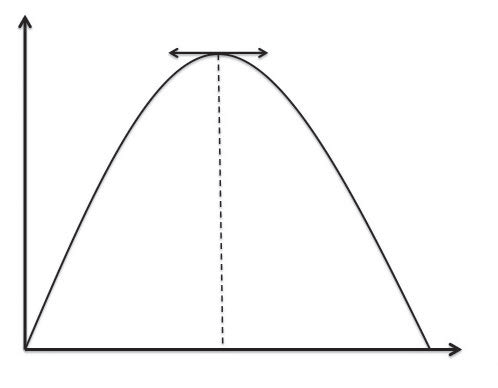
\includegraphics[width=0.75\textwidth]{4º Período/História do Pensamento Econômico/Tradução HPE/Tradução Tópico 9.3/figura 1.png}
    \end{figure}

Os sociólogos construtivistas da ciência reconhecerão na descrição anterior a rigorosa demarcação entre o status comunicacional da curva de Laffer como uma representação visual, de um lado, e as virtudes científicas do embasamento matemático que se pode aplicar a ela, de outro lado, uma curiosa variante do "modelo de difusão" que eles têm criticado ao longo dos últimos 25 anos. Neste modelo, conceitos e ferramentas são inicialmente inventados por gênios cujas reputações vão muito além de seu modesto status como cientistas atuantes. Essas inovações então se difundem para públicos maiores — outros cientistas, estudantes e o público em geral — por meio de um processo que parece automático: as ações de muitos indivíduos e grupos na aceitação e adoção dessas inovações são consideradas garantidas, e as muitas controvérsias que as descobertas geraram inicialmente são geralmente atenuadas e retratadas como ruídos inevitáveis, embora indesejáveis, no processo de difusão. À luz do modelo de difusão, a curva de Laffer é um caso muito estranho porque, pelo menos na descrição dos livros didáticos, sua aceitação parece ter funcionado ao contrário. Em vez de um gênio como os Pasteurs e Diesels do passado, o inventor da curva, Arthur Laffer, frequentemente nem sequer é reconhecido com o título de economista (embora certamente o seja). Os verdadeiros heróis da história são os pesquisadores anônimos trabalhando "a jusante", que forneceram as evidências de que a curva não é empiricamente validada. Mas, estranhamente, apesar do ataque heroico dos autores do livro didático contra a falsidade óbvia da curva de Laffer, a curva ainda está presente no livro, exibida em sua versão canônica e simétrica. Ficamos com uma pergunta que o modelo de difusão não consegue abordar de maneira satisfatória: como ela persistiu?

Talvez um dos modelos alternativos que os sociólogos elaboraram em resposta ao modelo de difusão ofereça uma estrutura melhor para pensar sobre a curva de Laffer. No modelo de "dispersão" — ou "tradução" —, fatos e ferramentas viajam dentro de várias comunidades através do espaço e do tempo. As atitudes que essas diferentes comunidades têm em relação aos objetos que viajam — aceitação, desafio, ignorância ou interesse — diferem muito dependendo de várias contingências. Para serem capazes de viajar, os objetos precisam ser transformados para se adequarem a novos constituintes. Como resultado, sua forma, significado e funcionamento serão afetados, assim como seu status epistemológico. No processo, as atitudes das pessoas que interagem com eles provavelmente evoluirão também (veja Latour 1987, 139–140). Nos últimos anos, vários historiadores da ciência seguiram essa estrutura para construir narrativas mais ricas da disseminação de representações visuais em várias disciplinas. A descrição de David Kaiser (2005) dos diagramas de Feynman na física depende explicitamente do modelo de dispersão, que, em sua opinião, integra duas dimensões importantes dos objetos que estuda: como eles circulam e como persistem. Além disso, historiadores argumentaram que as representações visuais devem ser estudadas na intersecção de dicotomias bem estabelecidas — laboratórios versus museus, artes versus ciências, geometria versus álgebra —, pois é frequentemente no diálogo entre essas que a visualização é discutida (Wise 2006).

O propósito deste capítulo é fornecer um relato histórico da curva de Laffer como um estudo de caso de dispersão. Parece ser um caso ideal para isso porque, como sugeri anteriormente, a trivialidade formal da curva contrasta acentuadamente com a complexidade de sua circulação entre e entre diferentes comunidades: economistas, assessores políticos, propagandistas e jornalistas. Para cada uma dessas comunidades — que, além disso, não eram necessariamente homogêneas dentro de si mesmas —, a curva de Laffer tinha diferentes encarnações e significados; portanto, faz mais sentido usar o plural curvas em vez do singular. No entanto, veremos que a dispersão das curvas de Laffer apresentou duas peculiaridades: primeiro, ao contrário de muitos outros diagramas usados na economia, as instâncias populares da curva de Laffer precederam sua "academização" por economistas profissionais; segundo, apesar das numerosas transformações que a curva sofreu no processo de sua circulação, sua apresentação canônica — a curva simétrica em forma de bala na figura 13.1 — foi reforçada ao longo do tempo. A circulação das curvas de Laffer deve ser explicada pela dinâmica interna de cada uma das comunidades que interagiram com elas, e pelo que acontece na intersecção dessas comunidades, mais importante como consequência da posição ambígua que a profissão econômica manteve em relação ao seu papel na assessoria política. Embora a disciplina sempre tenha estado ansiosa para oferecer conhecimento mais legítimo — do ponto de vista científico — do que o que é circulado em jornais e panfletos, ela também teve que encontrar legitimidade como uma ciência orientada para políticas. Começarei retratando as origens políticas da curva (seção 2); então, passarei para sua subsequente "academização" (seção 3) e generalização (seção 4). Como a discussão a seguir será principalmente histórica em seu conteúdo, discutirei na conclusão algumas implicações para a sociologia do conhecimento e, mais especificamente, para o estudo de práticas representacionais na economia.

\subsubsection{\textbf{O Significado Político da Curva de Laffer Original}}

A curva de Laffer não se originou na literatura acadêmica, e Arthur B. Laffer foi apenas parcialmente responsável por sua circulação. Ela foi, de fato, introduzida por Jude Wanniski em seu livro de 1978 \textit{The Way the World Works}. Nascido em 1936, Wanniski foi contratado como colunista do \textit{Wall Street Journal} em 1972, após anos cobrindo a política energética para vários jornais. Quando seu livro foi lançado, ele acabara de ser forçado a renunciar a essa posição depois que foi descoberto que ele estava distribuindo panfletos para um candidato republicano ao senado. Ele decidiu começar uma carreira como assessor de vários políticos republicanos e criou um negócio para isso, a Polyeconomics. Wanniski era conhecido como um ardente defensor da ``economia de oferta'', um termo que ele havia cunhado em 1976 em contraste com a ênfase do lado da demanda na economia keynesiana sobre a intervenção governamental para estimular o consumo privado e o investimento e reduzir o desemprego. A economia de oferta foi defendida por dois professores de economia, Robert Mundell e Arthur Laffer, que argumentaram que a intervenção estatal tinha efeitos prejudiciais sobre a oferta de bens e mão de obra e era a principal causa da redução do PNB e do aumento do desemprego. Embora Mundell, um ex-estudante de doutorado no MIT que havia lecionado na Universidade de Chicago até 1971, fosse respeitado entre os economistas por seus modelos macroeconômicos internacionais, ele estava se tornando marginalizado na profissão nos anos 1970 após sua produção científica ter diminuído. Laffer, por outro lado, era considerado entre os colegas economistas como um jovem estudioso promissor que havia praticamente cessado o trabalho acadêmico para seguir uma carreira mais politicamente orientada. Depois de estudar em Yale e Stanford e ensinar na escola de negócios de Chicago, ele havia servido como assessor econômico para as administrações Nixon e Ford. De acordo com Wanniski, Laffer havia desenhado a curva que levaria seu nome em um guardanapo de coquetel durante uma reunião com alguns assessores presidenciais em dezembro de 1974.


\begin{figure}[H]
    \centering
    \caption{Gráfico 13.2}
    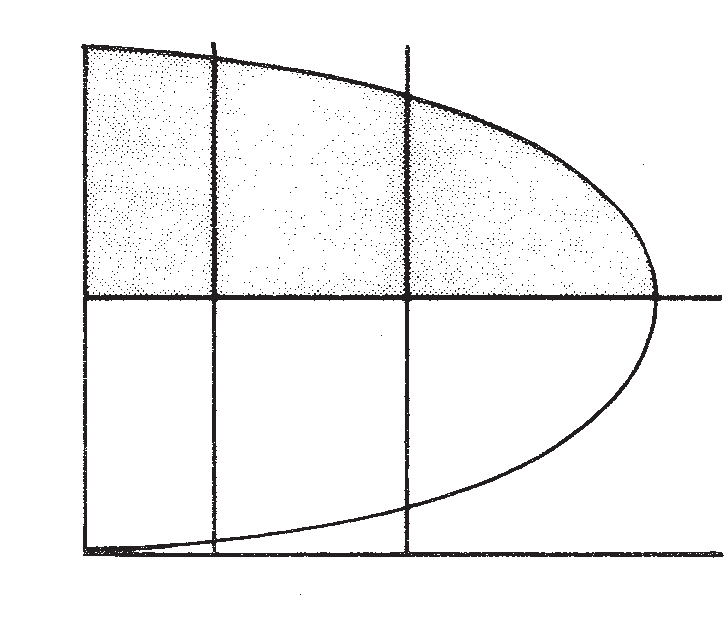
\includegraphics[width=0.75\textwidth]{4º Período/História do Pensamento Econômico/Tradução HPE/Tradução Tópico 9.3/figura 2.png}
    \end{figure}

Na sua representação original, a curva de Laffer apareceu como um diagrama em forma de bala, no qual as receitas fiscais eram representadas no eixo horizontal e a taxa tributária agregada no eixo vertical (figura 13.2). Nas palavras de Wanniski, a curva ilustra a ideia de que ``sempre existem duas taxas tributárias que geram as mesmas receitas'' (Wanniski 1978, 97). Enquanto a parte inferior da curva representa uma relação crescente entre as taxas tributárias e as receitas fiscais, essa relação torna-se decrescente além do ponto E. A interpretação dessa relação é que, quando as taxas tributárias aumentam de zero até qualquer porcentagem abaixo do ponto E, os agentes econômicos pagarão seus impostos mantendo inalterada a sua oferta de trabalho e bens. Nessa faixa inferior, taxas tributárias mais altas gerarão maiores receitas fiscais. No ``intervalo proibitivo'', no entanto, que é a parte além do ponto E, as pessoas decidirão trabalhar menos ou participar de uma economia de escambo (ou negra), o que levará a uma redução da base tributária e subsequente diminuição das receitas fiscais. O ponto E, portanto, aparece como o ponto em que as receitas fiscais seriam máximas. Esse ponto, Wanniski observou, é um ``número variável. É o ponto em que o eleitorado deseja ser tributado... É tarefa do líder político determinar o ponto E e segui-lo em suas variações o mais de perto possível'' (ibid., 98–99, ênfase no original).

Wanniski colocou a curva de Laffer no centro de seu livro de 1978, cuja publicação foi apoiada por Irving Kristol, um ex-colega no \textit{Wall Street Journal} e uma das principais figuras do então emergente movimento neoconservador. A aprovação da Proposição 13 na Califórnia em junho de 1978, que resultou em uma redução drástica das taxas de imposto sobre a propriedade naquele estado, foi seguida por revoltas fiscais em todo o país. Na preparação para as eleições de meio de mandato e a próxima campanha presidencial, havia uma clara percepção entre os republicanos de que era necessário mais do que o discurso conservador tradicional, que defendia um corte nos gastos governamentais e controles sobre preços e salários para estabilizar a inflação. Para esse propósito, a curva de Laffer era oportuna. Ao contrário do discurso direitista ortodoxo da época, que tentava convencer a população de que sacrifícios eram necessários no caminho para o crescimento econômico, a curva de Laffer sugeriu que menos tributação resultaria em mais riqueza para distribuir. Como resultado, economistas do lado da oferta não defendiam um corte no investimento público: ao contrário, um corte de impostos que contribuísse para aumentos nas receitas fiscais permitiria mais gastos governamentais no futuro. Essa foi, em linhas gerais, a ``economia da alegria'' que dominou a campanha de Ronald Reagan a partir de 1978 (Stein 1984).


O livro de Wanniski e a curva de Laffer que ele promoveu forneceram um trampolim para a propaganda do lado da oferta, baseando-se em um populismo antiexperts e na crítica à profissão econômica como um todo. Wanniski argumentou no início de seu livro que os eleitores sabiam mais do que os economistas, no sentido de que seu próprio comportamento poderia contradizer as previsões dos especialistas. Nessa crítica, economistas acadêmicos foram repreendidos junto com conselheiros econômicos por fornecerem teorias irrelevantes e conselhos equivocados. Na visão de Wanniski, a curva de Laffer personificava a falha dos economistas — exceto Mundell e Laffer, claro — em perceber que havia uma fronteira tênue entre uma economia monetária e uma economia de escambo, entre trabalho e não trabalho. O resto do livro tentava demonstrar que a história econômica — desde o declínio do Império Romano até crises econômicas passadas e presentes — poderia ser interpretada usando a curva de Laffer e que as teorias econômicas passadas também poderiam ser encapsuladas usando o arcabouço da curva. No capítulo 8, o autor atacou Keynes e seus principais oponentes, Milton Friedman e os monetaristas da Escola de Chicago. Enquanto a defesa de Keynes pelo gasto deficitário sem cortes de impostos lançaria a economia na faixa proibitiva da curva de Laffer, o apelo de Friedman por um corte nos gastos governamentais resultaria em um aumento nas taxas de juros que, por sua vez, contrabalançaria os efeitos esperados das reduções de impostos. Wanniski argumentou que o que tornava esses dois arcabouços igualmente inválidos era que ambos modelavam a economia em termos de análise de equilíbrio parcial, referindo-se a Alfred Marshall, que analisava um mercado de cada vez. Em contraste, seu próprio modelo, a curva de Laffer, seguiria o arcabouço de equilíbrio geral de Léon Walras, onde todos os efeitos econômicos eram considerados simultaneamente. É por isso que, segundo Wanniski, apenas Laffer e Mundell estavam corretos em sua abordagem, enquanto outros economistas estavam construindo ``edifícios matemáticos elegantes sobre uma fundação de ilusão'' (ibid., 166). Isso constituía nada menos que um insulto à maioria dos economistas mainstream do período pós-guerra, que afirmavam ter revivido a tradição Walrasiana, que, por sinal, era mais, não menos, matemática do que a análise Marshalliana que a maioria havia abandonado.

Diante de tais comentários depreciativos, a maioria dos economistas permaneceu em silêncio. Nenhuma resenha de \textit{The Way the World Works} foi publicada em periódicos acadêmicos de economia, apesar do fato de que tais revistas frequentemente dedicavam espaço à literatura não acadêmica. Admitidamente, alguns economistas expressaram sua desaprovação da curva de Laffer, mas apenas quando escreviam na imprensa popular. Por exemplo, Joseph Minarik foi citado no \textit{New York Times} afirmando que ele havia feito o cálculo e encontrado resultados demasiadamente erráticos para certificar que a curva existia; ``seus projetistas deveriam alisar algumas das rugas antes de oferecê-la ao público'' (Rattner 1978). Até mesmo Laffer recuou um pouco do entusiasmo de Wanniski. Quando questionado por um jornalista para explicar sua curva, ele a apresentou como incorporando dois efeitos conflitantes que as taxas de impostos têm sobre as receitas fiscais: um era o efeito ``aritmético'' ou ``contábil'', que implicava que impostos mais baixos levariam a uma diminuição na receita coletada por dólar de base tributária; e o outro era o ``efeito econômico'', que resultava em uma expansão da base tributária. No entanto, ele não concluiu qual efeito dominaria o outro (citado em Jensen 1978). Em 1979, três dos estudantes de Laffer na Universidade do Sul da Califórnia publicaram um artigo curto no qual tentavam construir uma versão mais elaborada da curva, usando apenas raciocínio diagramático (Canto, Joines e Webb 1979). Neste modelo, a curva foi derivada de um modelo microeconômico uma vez aceito no qual um aumento nas taxas de impostos cria incentivos para se mover do setor de mercado (trabalho) para o setor doméstico (lazer). Este modelo, no entanto, constituiu um sério retrocesso em relação às ambições de Wanniski. Ele ignorou muitas das complexidades em um arcabouço Walrasiano generalizado e baseou sua análise em uma única taxa de imposto imposta sobre a produção do setor de mercado. Além disso, os estudantes realizaram testes empíricos bastante decepcionantes: usando os cortes de impostos de 1962 e 1964 como um experimento, eles tiveram que concluir que era ``quase igualmente provável que os cortes de impostos de Kennedy aumentassem as receitas como que as diminuíssem'' (ibid., 38). Dois artigos subsequentes (Canto, Joines e Laffer 1981; Laffer 1981) tentaram construir modelos mais elaborados de tributação, mas nenhum deles incluiu uma curva de Laffer real. Essas contribuições, que não apareceram em periódicos de economia mainstream, não conseguiram alcançar os economistas acadêmicos. Estes, de fato, consideravam o debate sobre a curva de Laffer como uma distração indesejável do pensamento econômico sério.

\subsubsection{\textbf{A "Academização" da Curva}}

Demorou cerca de três anos até que a curva de Laffer penetrasse na literatura acadêmica. Nesse ínterim, Ronald Reagan se tornou presidente e sua administração já havia tomado medidas para reduzir os impostos. Os economistas da escola de oferta foram bastante influentes nas reformas fiscais. Atuando como consultor do congressista de Nova York, Jack Kemp, Wanniski ajudou a elaborar a proposta de corte de impostos Kemp-Roth de 1978, que serviu de base para a Lei de Recuperação Econômica (ERTA) de 1981. O projeto que foi aprovado pelo Congresso, no entanto, representou um pequeno recuo do plano inicial de Kemp: enquanto Kemp havia aconselhado um corte de impostos de 33\%, aplicado uniformemente a todas as faixas de impostos, a ERTA reduziu as taxas máximas de 70 para 50\% e as taxas mínimas de 14 para 11\%. Embora a reforma tributária não tenha seguido escrupulosamente as prescrições da curva de Laffer, esta ainda era vista como um de seus principais componentes ideológicos na imprensa popular. O aumento das receitas fiscais que os economistas da escola de oferta haviam previsto não ocorreu, e os cortes de impostos resultaram em déficits orçamentários e esforços subsequentes para cortar gastos. Um desses esforços envolveu uma proposta para cortar o financiamento das ciências sociais e comportamentais em 75\%. Escrito por David Stockman, chefe do Escritório de Orçamento e Gestão, ele pressagiava um dano significativo à pesquisa econômica, que dependia fortemente de bolsas da Fundação Nacional de Ciências. O comitê executivo da Associação Econômica Americana, que geralmente evitava questões políticas, expressou preocupações sobre a situação. Seu presidente, William Baumol, escreveu uma carta aos presidentes dos departamentos de economia nos Estados Unidos, incentivando-os a escrever aos membros do Congresso para alertá-los sobre as consequências prejudiciais que tais cortes teriam na busca pelo conhecimento econômico. Em 1981, então, o evangelho dos economistas da escola de oferta estava ameaçando materialmente a comunidade econômica. Como se isso não fosse ruim o suficiente, a saga dos "fracassados" cortes de impostos também estava transformando toda a profissão em motivo de riso aos olhos de outros cientistas e intelectuais, que consideravam a curva de Laffer não apenas um exemplo particularmente fraco de pensamento econômico, mas também um sintoma de que a economia em si era mera ideologia respaldada por matemática medíocre. Característico dessa posição foi a publicação na Scientific American de um artigo de Martin Gardner, um conhecido especialista em matemática recreativa, intitulado "A Curva de Laffer e Outras Risadas na Economia Atual". Zombando do argumento de Wanniski de que o ponto E poderia ser localizado em qualquer lugar ao longo da curva, Gardner introduziu a curva neo-Laffer (figura 13.3). "Como a velha curva de Laffer", escreveu ele, "a nova também é metafórica, embora seja claramente um modelo melhor do mundo real. Como é um reflexo estatístico do comportamento humano, sua forma muda constantemente, como a curva de Phillips, de maneiras imprevisíveis" (Gardner 1981, 27). Gardner não apenas satirizou a curva de Laffer original, mas também zombou de tentativas posteriores de tirar estimativas da curva: "Porque leva muito tempo para reunir dados e ainda mais para analisar todos os parâmetros de mudança, quando uma curva NL é desenhada, ela está desatualizada e não é muito útil" (ibid.).

\begin{figure}[H]
    \centering
    \caption{Gráfico 13.3}
    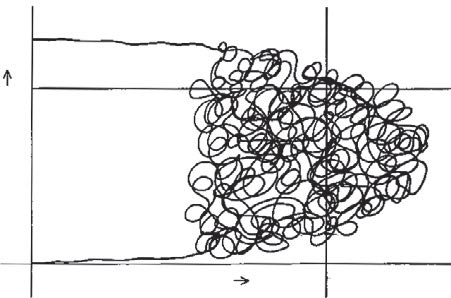
\includegraphics[width=0.75\textwidth]{4º Período/História do Pensamento Econômico/Tradução HPE/Tradução Tópico 9.3/figura 3.png}
    \end{figure}

Enquanto isso, dentro da administração Reagan, havia um crescente descontentamento com a economia da oferta. Entre os conselheiros, monetaristas como Arthur Burns e Alan Greenspan ainda acreditavam que o controle da oferta monetária por meio do aumento das taxas de juros deveria prevalecer sobre os cortes de impostos como forma de garantir o crescimento econômico a longo prazo. O monetarismo, de fato, era o principal princípio que havia orientado as ações do Federal Reserve desde 1979, quando Paul Volcker foi nomeado presidente. Em contraste, os verdadeiros crentes na economia da oferta estimaram que a política monetária atual havia impedido que os cortes de impostos rendessem as receitas esperadas. À medida que as tensões aumentavam, o debate político se tornava desagradável. Wanniski, por exemplo, escreveu em julho de 1981: “Milton Friedman não é um homem grande, mas é muito pesado. Suas ideias econômicas monetaristas... estão prejudicando o velho amigo do laureado com o Nobel, Ronald Reagan, a economia dos Estados Unidos e, indiretamente, todos os nossos parceiros comerciais. O professor Friedman tem pouco mais de um metro e meio de altura, mas sua sombra se estende pela última década de inflação global” (Wanniski, 1981). Em reação a tanta acrimônia, muitos economistas sentiram que era hora de uma investigação acadêmica mais séria sobre a curva de Laffer, que não apenas levaria o debate em uma direção mais rigorosa, mas também restauraria a credibilidade da profissão econômica. A resposta dos economistas, naturalmente, implicava no aumento da matematização dos modelos concorrentes. Duas contribuições, publicadas em 1982, provaram ser particularmente influentes em trazer a curva de Laffer para o debate acadêmico.

Primeiro, Don Fullerton (1982) ofereceu um modelo analítico completo da curva que a tornaria uma hipótese testável. Ele observou que, enquanto a típica curva de Laffer representa como as receitas fiscais variam com as mudanças nas taxas de impostos, o fator-chave para determinar se estamos na faixa normal ou proibitiva é a elasticidade da oferta do fator: o grau em que uma variação no imposto afetará a oferta do fator - trabalho ou capital - sendo tributado. Como resultado, uma infinidade de curvas de Laffer pode ser imaginada - com uma curva para cada valor de um dado fator de oferta elástica. Fullerton, portanto, postulou que a curva de Laffer não era uma "colina", como a representação canônica mostrava, mas uma "cordilheira", já que tinha que ser representada em um diagrama tridimensional com a elasticidade da oferta do fator como a terceira dimensão. Fullerton só desenhou o "cume" da cordilheira, que mostrava uma relação descendente entre as taxas de impostos e a elasticidade da oferta do fator, representando cada ponto ao longo da curva onde as receitas fiscais seriam máximas (veja a figura 13.4). A faixa normal está localizada abaixo da curva, enquanto a área acima da curva corresponde à faixa proibitiva. Usando um modelo econométrico de equilíbrio geral dos Estados Unidos, Fullerton tentou estimar a nova curva e eventualmente a forma das curvas de Laffer para várias taxas de impostos e elasticidades de oferta de fatores. Ele concluiu que, em teoria, os EUA poderiam estar operando na faixa proibitiva no caso em que os salários são tributados a uma taxa muito alta. No entanto, levando em conta as estimativas econométricas anteriores das elasticidades da oferta de trabalho para vários grupos da população, ele mostrou que, sob suposições realistas, a taxa de imposto proibitiva teria que ser bem acima da taxa atual nos EUA. Em outras palavras, a curva de Laffer começaria a diminuir a uma taxa de imposto muito mais alta do que as representações anteriores sugeriam.

\begin{figure}[H]
    \centering
    \caption{Gráfico 13.4}
    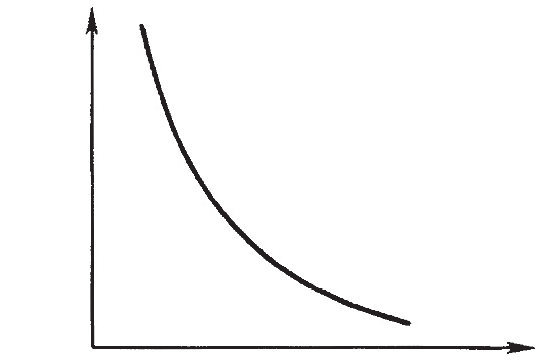
\includegraphics[width=0.75\textwidth]{4º Período/História do Pensamento Econômico/Tradução HPE/Tradução Tópico 9.3/figura 4.png}
    \end{figure}

O breve artigo de James Buchanan e Dwight Lee (1982) constituiu uma abordagem completamente diferente para a curva de Laffer. Os autores não tentaram questionar suas fundações, mas sim suas consequências dentro do arcabouço econômico da teoria da escolha pública. Ao contrário da maioria dos economistas, que presumiam que o Estado era um observador externo operando em favor de resultados socialmente desejados, os teóricos da escolha pública argumentavam que o governo consistia em agentes econômicos que maximizavam a utilidade e agiam em benefício próprio. A partir deste ponto de partida, Buchanan e Lee procuraram explicar como um governo supostamente racional acabaria escolhendo uma taxa de imposto menos do que ótima. Sua resposta consistiu em argumentar que a curva de Laffer que outros haviam tentado avaliar até agora era, na verdade, a representação de uma relação que só ocorreria a longo prazo, enquanto o governo estava mais propenso a agir de acordo com objetivos de curto prazo. Em sua estrutura, a diferença entre os efeitos de curto e longo prazo é o tempo que leva para os contribuintes se ajustarem às mudanças na tributação. Visualmente, sua representação (figura 13.5) consiste em uma curva de Laffer de longo prazo (LRLC) e várias curvas de Laffer de curto prazo (SRLC). Para cada ponto localizado na LRLC, existe uma SRLC diferente que é mais favorável ao governo. Isso significa que, como os contribuintes não ajustam totalmente seu comportamento à taxa de imposto existente no curto prazo, é sempre melhor para o governo aumentar sua taxa de imposto acima do nível que renderia receitas máximas a longo prazo. No entanto, o governo tem que escolher uma taxa de imposto localizada na LRLC porque é a única maneira de garantir uma base tributária. Se a taxa de imposto estivesse localizada além da curva, não haveria renda para tributar. Eventualmente, a taxa de imposto escolhida será aquela que renderá receitas máximas em uma SRLC e que está simultaneamente localizada em algum lugar na porção decrescente da LRLC. Esta situação, argumentam Buchanan e Lee, é estável porque não há incentivo para o governo reduzir seus impostos no curto prazo, que é o único horizonte de planejamento com o qual se preocupa. Portanto, a situação não ótima vai persistir ao longo do tempo. A contribuição de Buchanan e Lee foi particularmente impressionante: ao contrário das tentativas anteriores de aprofundar as implicações analíticas da curva de Laffer, sua versão desta envolveu nenhum outro formalismo matemático além de sua representação diagramática. A razão para isso é que os autores, ao contrário de Fullerton (1982), não estavam interessados em questionar a forma da curva de acordo com dados do mundo real. Em vez disso, eles se concentraram na mera possibilidade de que a curva exista. Ao fazer isso, eles puderam abordar uma questão de teoria política: como governos racionais acabam agindo contra seus próprios interesses? Nesse sentido, a curva de Laffer apareceu não como um modelo que precisa de refinamento, mas como um motor de descoberta.

    \begin{figure}[H]
    \centering
    \caption{Gráfico 13.5}
    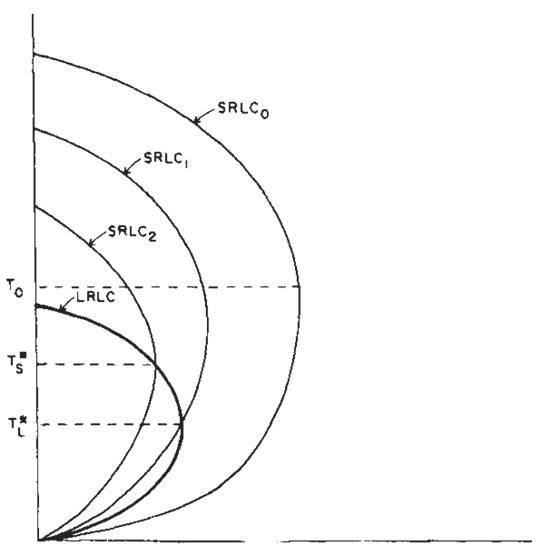
\includegraphics[width=0.75\textwidth]{4º Período/História do Pensamento Econômico/Tradução HPE/Tradução Tópico 9.3/figura 5.png}
    \end{figure}

Embora tenham levado a curva de Laffer em duas direções diferentes, as respectivas contribuições de Fullerton e Buchanan e Lee participaram de sua legitimação como uma ferramenta acadêmica, fornecendo um ponto de partida respeitável para pesquisas futuras.

\subsubsection{\textbf{A Generalização das Curvas de Laffer}}

É impressionante que justamente no momento em que a curva de Laffer foi atacada como um projeto político, ela começou a atrair cada vez mais atenção dos economistas acadêmicos. Em 1986, embora novos cortes de impostos estivessem sendo preparados, a curva de Laffer havia praticamente desaparecido do debate público. Em 1984, Herbert Stein, ex-conselheiro econômico de Nixon, resumiu o sentimento geral: "Entre 1981 e 1983, o país passou de um entusiasmo efervescente pela redução de impostos para um triste reconhecimento de que os impostos eram muito baixos - que somos... uma sociedade subtributada" (Stein 1984, 356). No livro de Stein, a curva de Laffer foi representada como uma curva em forma de sino acentuadamente assimétrica, com a mudança da faixa normal para a faixa proibitiva ocorrendo aproximadamente a uma taxa de imposto de 80\%. Stein observou: "A imagem convencional na qual a curva é simétrica e atinge seu ponto alto a 50\% tem apenas uma justificativa estética" (ibid., 247). No entanto, a mesma curva de Laffer simétrica foi posteriormente dispersa pela literatura científica ao longo de três diferentes linhas de desenvolvimento: primeiro, como base para hipóteses econométricas adicionais; segundo, para explorações mais profundas de sua análise subjacente; e finalmente, para aplicações além das finanças públicas.

Na primeira linha, para o desenvolvimento de hipóteses testáveis, a curva de Laffer não assumiu muita importância. Na verdade, a dificuldade em fazer estimativas empíricas a partir dela era que havia muitas variáveis que tinham que ser simplificadas ou ignoradas: mudanças na distribuição de renda, a complexidade das estruturas tributárias, a forma como as receitas fiscais eram redistribuídas entre os contribuintes, etc. Consequentemente, as estimativas empíricas do pico variavam de um estudo para outro, cobrindo uma faixa entre 40 e 90\%. Além disso, o modelo da curva de Laffer não fornecia uma base clara para comparar tais estimativas entre si. Uma solução foi passar de testar a curva de Laffer para tratar as consequências da vida real de cortes de impostos específicos como descobertas experimentais. Foi isso que Austan Goolsbee, economista da Universidade de Chicago, fez em 1999. Estudando várias mudanças de impostos na história dos EUA, Goolsbee argumentou que nenhum efeito particular sobre as receitas poderia ser identificado que informaria a política. Ele concluiu que "[a] noção de que os governos poderiam arrecadar mais dinheiro cortando as taxas é, de fato, uma ideia gloriosa... Infelizmente para todos nós, os dados do registro histórico sugerem que é improvável que seja verdade em algo como as taxas marginais de impostos de hoje" (Goolsbee 1999, 44). O que é interessante aqui para o nosso propósito é que Goolsbee, embora tenha se referido à curva de Laffer em todo o seu artigo, na verdade não testou a curva, mas apenas a ideia de que taxas marginais de impostos mais altas podem reduzir as receitas do governo. O alvo de Goolsbee, na verdade, era Martin Feldstein, um economista com credenciais acadêmicas mais sólidas do que Laffer. Feldstein havia fornecido justificativas teóricas para a redução de impostos já no meio da década de 1970 e havia se envolvido na reforma tributária durante o segundo mandato de Reagan, precisamente quando os economistas da oferta haviam perdido sua influência no governo. Goolsbee (1999, 9) distinguiu o trabalho acadêmico de Feldstein da "curva de Laffer convencional", que ele disse "não existe". Ele não citou nenhum artigo de Laffer, não reproduziu a famosa curva em lugar algum de seu artigo, e não fez nenhuma referência à versão, até então, quase universalmente ridicularizada que Wanniski e outros economistas da oferta haviam oferecido no final da década de 1970. Em uma seção de discussão e comentário publicada com o artigo, Robert E. Hall começou observando que Laffer não deveria ter sido mencionado no título de forma alguma (em Goolsbee 1999, 48). No entanto, o que o artigo de Goolsbee sinalizou foi que, no final da década de 1990, o termo "curva de Laffer" havia se desvinculado um pouco de suas origens para servir como uma marca registrada para o argumento academicamente respeitável de que cortes de impostos, ao aumentar a oferta de trabalho, ajudariam a aumentar tanto as receitas nacionais quanto governamentais.

O segundo tipo de estudo acadêmico tentou explorar as complexidades analíticas mais profundas da curva de Laffer. Em vez de tentar estimar onde o pico da curva ocorreria, esses estudos mostraram um interesse crescente na questão de se um ponto de mudança ocorre, e portanto questionaram a forma da própria curva. Malcomson (1986), por exemplo, estudou a possibilidade de que a curva inclinasse para cima para todas as taxas médias de impostos. Essa discussão foi perseguida nas páginas do Journal of Public Economics entre 1986 e 1991. Gahvari (1989) provou que no arcabouço de Malcomson, uma condição suficiente para a curva ter uma parte descendente é que a receita tributária seja redistribuída aos contribuintes na forma de uma soma fixa. Guesnerie e Jerison (1991) tentaram generalizar a curva de Laffer sugerindo que ela poderia ser substituída por uma infinidade de curvas correspondentes a várias funções de receita tributária em um arcabouço de equilíbrio geral. Embora seu artigo dissesse que era impossível tirar conclusões de política, porque era impossível prever se uma diminuição nas taxas de impostos resultaria em maiores receitas fiscais, sua principal contribuição foi ampliar a relevância da curva de Laffer. Enquanto no modelo original de Laffer o foco havia sido exclusivamente nas receitas fiscais, Guesnerie e Jerison argumentaram que um arcabouço de equilíbrio geral deveria se concentrar no bem-estar social também. Como as receitas fiscais são usadas para financiar bens públicos, taxas de impostos mais altas resultarão em dois efeitos conflitantes: primeiro, taxas mais altas aumentarão o bem-estar social, porque as pessoas se beneficiarão dos bens públicos adicionais; mas, em segundo lugar, o aumento resultante nos preços dos bens privados terá um efeito prejudicial ao bem-estar social. Isso leva a múltiplos equilíbrios possíveis que renderiam receitas fiscais máximas, mas será praticamente impossível saber quais taxas realmente maximizariam o bem-estar social. Ao buscar generalização e rigor analítico, esses modelos dependem de formalismos cada vez mais complexos. Embora indubitavelmente tenham demonstrado que a versão didática da curva de Laffer era um caso especial de uma relação mais geral com pouca chance de ocorrer na vida real, eles também ajudaram a substanciar a afirmação de que a curva poderia existir em teoria. Em consequência, no final da década de 1990 era muito provável que se deparasse com curvas de Laffer padrão na literatura mainstream.

Um terceiro aspecto do uso da curva de Laffer na literatura econômica recente foi derivado do modelo Buchanan-Lee de 1982, que ofereceu o arcabouço mais facilmente transponível para estudar casos práticos. Um exemplo significativo é um artigo de Clark e Lee (1996), que invoca a curva de Laffer em um estudo sobre política de sentença criminal. Seu artigo traçou a "curva de Laffer de sentença" para cada comprimento médio de sentença que exigia espaço prisional (figura 13.6). De acordo com seu modelo, uma redução no comprimento médio da sentença, que normalmente deveria reduzir a necessidade de espaço prisional, poderia levar ao efeito oposto, à medida que as taxas de criminalidade aumentam em resposta a maiores incentivos para violar a lei. Usando uma análise bastante semelhante à de Buchanan e Lee (1982), Clark e Lee mostraram que o governo provavelmente escolheria um comprimento médio de sentença ineficientemente baixo que não minimizaria a necessidade de espaço prisional. Como no modelo Buchanan-Lee, essa situação subótima pode persistir, porque a curto prazo o governo não teria interesse em estender os comprimentos das sentenças.

\begin{figure}[H]
    \centering
    \caption{Gráfico 13.6}
    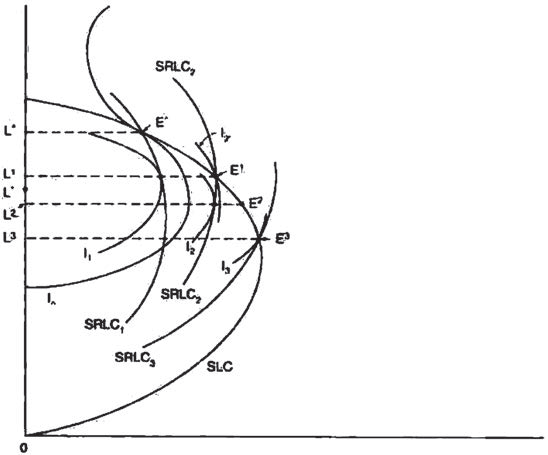
\includegraphics[width=0.75\textwidth]{4º Período/História do Pensamento Econômico/Tradução HPE/Tradução Tópico 9.3/figura 6.png}
\end{figure}

Shmanske (2002) forneceu outra aplicação do arcabouço de Buchanan-Lee, desta vez em um estudo sobre a economia da educação. O ponto de partida de Shmanske era a noção de que algumas escolas poderiam aliviar a carga de seu currículo na expectativa de que isso alcançaria um nível mais alto de matrículas. No entanto, além de um certo ponto, eles acabariam com matrículas insuficientes por causa da degradação da reputação da escola. Além disso, tal degradação impediria a escola de endurecer seu currículo no futuro, porque não seria suficientemente crível para fazê-lo. Tais aplicações metafóricas da curva de Laffer além do domínio das finanças públicas começaram a aparecer em publicações acadêmicas em meados da década de 1990. Na imprensa popular, também houve indicações de tal uso metafórico desde o final da década de 1980. No New York Times, o político democrata Ed Markey (1988) se referiu a uma "versão termonuclear da curva de Laffer", que ele explicou como a noção paradoxal de que "[s]ob Reagatomics, agora construímos mais armas nucleares e melhoramos nossas capacidades de primeiro ataque para ter menos armas nucleares e reduzir a ameaça de um primeiro ataque nuclear desarmante." O uso da curva fora dos limites tradicionais da economia parecia atender a uma demanda social maior por modelos econômicos simples com implicações práticas para situações da vida real. Nesse contexto, a curva de Laffer se tornou uma metáfora difundida para explicar os erros de um governo supostamente racional.

\subsubsection{\textbf{Conclusão}}
John Maynard Keynes certa vez observou que os diagramas em economia compõem parte daquele "aparato elegante que geralmente exerce uma atração poderosa sobre os iniciantes inteligentes, que todos nós usamos como inspirador e um controle sobre nossas intuições e como um registro resumido de nossos resultados, mas que geralmente cai no esquecimento à medida que penetramos mais profundamente nos recessos do assunto" (Keynes 1924, 332 – 333). Relembrando a história da curva de Laffer, podemos concordar parcialmente com a observação de Keynes: a curva de Laffer exerceu fascínio sobre os "iniciantes inteligentes" — neste caso, principalmente não economistas — e serviu como um "inspirador" para modelos econômicos mais elaborados. No entanto, é mais difícil afirmar que a curva original caiu no esquecimento à medida que os modelos se tornaram cada vez mais técnicos, porque sua representação canônica parece ter sido reforçada no processo. Enquanto a narrativa anterior explicou como isso aconteceu nos últimos 30 anos, é hora de refletir sobre as razões para a circulação persistente da curva. Duas linhas de interpretação podem ser apresentadas, uma baseada no status da curva de Laffer como uma representação visual localizada na interseção entre pesquisa e política, e a outra envolvendo o contexto institucional específico que envolve sua circulação.

Esta breve história da curva de Laffer mostra que ela foi inicialmente concebida como uma representação simples de uma realidade que se supunha ser complexa: uma realidade que envolvia uma estrutura tributária complicada e tantos comportamentos diferentes quanto os contribuintes individuais poderiam adotar em resposta às mudanças nas taxas de impostos, sem mencionar os efeitos cumulativos que tais comportamentos poderiam gerar no nível macroeconômico. No entanto, os economistas não estavam em posição de criticar a pretensão de uma curva simples de retratar tais relações intrincadas, porque no passado recente eles haviam usado várias curvas igualmente simples para retratar o funcionamento da economia como um todo. Por que tais representações visuais simples são tão persistentes? A resposta é que enquanto a matematização subsequente de tais curvas simples pode aumentar sua credibilidade aos olhos dos pesquisadores mais teoricamente inclinados, também as torna cada vez menos atraentes para a política pública. No caso da curva de Laffer, sua simplicidade ajuda a explicar por que as versões mais matematicamente sofisticadas da curva não circularam amplamente, mesmo entre os economistas. Portanto, uma conclusão geral que pode ser tirada desta narrativa é que as representações econômicas que reivindicam forte relevância política e, consequentemente, atravessam a fronteira entre a pesquisa acadêmica e a política, provavelmente persistirão ao longo do tempo, apesar de, e talvez até por causa de, sua falha em resistir ao processo de refinamento técnico.

Ainda assim, a academização da curva de Laffer também deve ser entendida à luz do contexto sociológico e institucional mais amplo ao longo do último século que moldou o papel dos economistas na formulação de políticas nos Estados Unidos. Fourcade (2009) argumentou que o que era específico sobre a economia americana era seu enraizamento acadêmico, em contraste com o tipo mais burocrático de expertise econômica que prevalecia na Europa continental. A partir da década de 1930, na ausência de uma elite tecnocrática preexistente, os governos americanos passaram a depender cada vez mais de economistas acadêmicos para realizar várias tarefas técnicas. A legitimidade dos economistas como especialistas em políticas dependia das expectativas de seus sólidos padrões acadêmicos, mas também de sua capacidade de penetrar no mercado e vender suas habilidades por meio de organizações públicas e privadas sem fins lucrativos que não tinham agendas políticas definidas, como a Ford Foundation ou a Brookings Institution. Daí a relação dos economistas com a política era muitas vezes indireta e ambígua. A dispersão da(s) curva(s) de Laffer ocorreu na última parte do século XX, quando esse modelo de expertise econômica enfrentou uma crise, à medida que um novo tipo de think tank crudamente ideológico tentava competir com os economistas acadêmicos no mercado de expertise técnica. Quando alguns desses think tanks, como o Cato Institute com o qual Laffer e seus aliados estavam envolvidos, começaram a influenciar a política, a relação dos economistas com a política tornou-se ainda mais ambígua. Enquanto alguns economistas academicamente respeitáveis estavam interessados nesta nova oportunidade de disseminar suas ideias, outros estimaram que deveriam elevar ainda mais os padrões científicos de sua disciplina para fornecer um baluarte contra o que consideravam uma ameaça à sua legitimidade. Essas atitudes conflitantes podem explicar o desprezo que prevaleceu entre os economistas acadêmicos na recepção inicial da curva de Laffer, bem como sua posterior apropriação como um objeto de pesquisa aceitável. Enquanto, nas últimas duas décadas ou mais, os sociólogos da ciência procuraram mostrar que o estudo das representações na prática científica deve prestar atenção aos contextos sociais nos quais essas representações são produzidas, a história da curva de Laffer mostra que, para representações particulares, a noção de contexto teria que ser estendida para incluir os aspectos culturais, sociais e institucionais mais amplos que enquadram e legitimam o discurso científico.

\subsubsection{\textbf{Agradecimentos}}

Gostaria de agradecer a Béatrice Cherrier e José Edwards por me ajudarem a localizar alguns dos primeiros artigos sobre a curva de Laffer, Roger Middleton por compartilhar rascunhos não publicados e Fabian Gouret por comentários úteis. Além disso, me beneficiei de observações perspicazes, correções e referências adicionais fornecidas por três árbitros anônimos e pelos editores deste volume. As ressalvas habituais se aplicam.

\newpage
\section*{\textbf{Tópico 10}}
\addcontentsline{toc}{section}{Tópico 10}
\section{\textbf{Dequech (2008)}}
\subsection{\textbf{Economia neoclássica, mainstream, ortodoxa e heterodoxa}}

\subsubsection{\textbf{Resumo}}
Este artigo discute os conceitos de economia neoclássica, mainstream, ortodoxa e heterodoxa, distinguindo conceitos mais gerais e mais específicos temporalmente. O conceito de economia mainstream é baseado em prestígio e influência e inclui ideias ensinadas em escolas prestigiosas. Embora a corrente principal atual (incluindo a economia neoclássica) seja claramente diversa, a comunalidade nela é mais controversa. A economia heterodoxa pode ser definida negativamente, em oposição à ortodoxia ou à corrente principal. A falta de consenso gera problemas de comunicação. Outra possibilidade seria definir a economia heterodoxa positivamente, mas o resultado no período atual pode ser um conjunto vazio.

\subsubsection{\textbf{Palavras-chave}}

heterodoxo, mainstream, neoclássico, ortodoxo, escolas de pensamento

A economia, como outras ciências sociais, sempre foi marcada pela coexistência de diferentes escolas de pensamento (ou abordagens, etc.). Existem de fato diferenças significativas entre várias escolas, de modo que identificá-las e classificá-las é importante. Em seus exercícios de classificação, os economistas usaram uma infinidade de rótulos para designar essas escolas. Prefixos como "neo", "novo", "velho" e "pós" foram empregados. Às vezes, com ou sem esses prefixos, também foram usados adjetivos como clássico, institucionalista, e assim por diante. Outras vezes, os adjetivos escolhidos são derivados do nome de um indivíduo particular, como Ricardo, Marx, Walras, Keynes, Schumpeter, e assim por diante. Além da questão de como distinguir entre as escolas, essa última prática muitas vezes levanta a questão problemática de quão fiéis os membros de cada escola são ao pensamento de seu suposto pai fundador ou sua fonte de inspiração. Em um nível mais alto de generalidade estão rótulos como mainstream, ortodoxo e heterodoxo.

Os rótulos podem ser úteis, mas também podem ser confusos. De qualquer forma, seu uso parece inevitável, dada a considerável variação entre grupos de economistas e suas ideias. O presente artigo está preocupado com alguns dos rótulos mais gerais, especialmente com mainstream, heterodoxo e ortodoxo, bem como com um dos rótulos mais específicos - a saber, neoclássico.

Diferentes economistas usam esses termos de maneiras diferentes. Além disso, desenvolvimentos nas últimas duas ou três décadas tornaram a relação conceitual entre economia neoclássica e mainstream ainda mais complicada do que já era. Consequentemente, a definição de economia heterodoxa também se tornou mais problemática.

Além disso, o debate sobre o significado desses termos sofreu com uma frequente falta de clareza sobre o alcance temporal de aplicação dos conceitos. Em particular, às vezes os autores propõem um conceito sem especificar o período ou períodos a que se destina a aplicar; também acontece que os autores oscilam entre um conceito mais geral temporalmente e um conceito mais específico, sem deixar isso claro.

O presente artigo pretende contribuir para este debate, especificando diferentes conceitos e fazendo isso explicitando que alguns conceitos são temporalmente gerais, enquanto outros, geralmente referindo-se ao período atual, são temporalmente específicos.

\subsubsection{\textbf{Economia Neoclássica}}

Definir economia neoclássica não é fácil, principalmente porque o que se pode chamar de economia neoclássica mudou ao longo dos anos. Uma definição ampla se aplicaria à economia neoclássica original, fundada na década de 1870, bem como a trabalhos posteriores. Outra dificuldade é que mesmo em um dado momento, o termo não é necessariamente usado no mesmo sentido por todos.

O que é chamado aqui de economia neoclássica é caracterizado pela combinação das seguintes características:

1. a ênfase na racionalidade e o uso da maximização da utilidade como critério de racionalidade,

2. a ênfase no equilíbrio ou equilíbrios, e

3. a negligência de tipos fortes de incerteza e, particularmente, de incerteza fundamental.

Como veremos na próxima seção, a aderência estrita a essa caracterização não é necessária para estabelecer uma distinção entre economia neoclássica e mainstream, mas serve como uma aproximação muito boa.

\subsubsection{\textbf{Economia Mainstream}}

Um conceito interessante e útil de economia mainstream foi proposto por Colander, Holt e Rosser: para eles, "a economia mainstream... é em grande parte uma categoria definida sociologicamente. Mainstream consiste nas ideias que são mantidas por indivíduos que são dominantes nas principais instituições acadêmicas, organizações e revistas em qualquer momento dado, especialmente as principais instituições de pesquisa de pós-graduação. A economia mainstream consiste em ideias que a elite da profissão considera aceitável, onde por 'elite' entendemos os principais economistas nas melhores escolas de pós-graduação" (2004, p. 490). Pelo que entendo de Colander, Holt e Rosser, eles permitem que pessoas que não são membros da elite façam parte da economia mainstream; tudo o que é necessário é compartilhar as ideias da elite.

Em comparação com Colander, Holt e Rosser, eu prefiro uma variedade um pouco diferente do conceito sociológico de economia mainstream. Eu prefiro dizer que a economia mainstream é aquela que é ensinada nas universidades e faculdades mais prestigiosas, é publicada nas revistas mais prestigiosas, recebe fundos das fundações de pesquisa mais importantes e ganha os prêmios mais prestigiosos.

Existem algumas pequenas, mas possivelmente relevantes, diferenças entre essa maneira de descrever a economia mainstream e a de Colander, Holt e Rosser. Usar um conceito sociológico de economia mainstream, baseado em prestígio e influência, não requer que se foque tanto nas ideias da elite ou que se defina a elite de maneira tão restritiva quanto Colander, Holt e Rosser. Como esses autores apontam em uma discussão fascinante, a difusão de novas ideias entre o que eles chamam de elite ocorrerá vários anos ou até algumas décadas antes que essas ideias possam encontrar seu caminho nos livros didáticos de graduação, cujos conteúdos são mais resistentes à mudança (ibid., p. 494). Vamos imaginar, assim, uma situação em que as ideias de uma parte substancial da elite se tornaram bastante diferentes das ideias ensinadas no nível de graduação, mesmo nas universidades e faculdades mais prestigiosas. Se as últimas ideias são ensinadas em escolas prestigiosas, na minha opinião, elas ainda devem ser consideradas como parte da economia mainstream. Como o conceito pode se aplicar tanto a ideias quanto a pessoas (algo que Colander, Holt e Rosser também aceitam, na prática), os apoiadores dessas ideias também seriam elementos do conjunto de economistas mainstream. Por sua vez, isso permitiria que professores de cursos de graduação em universidades e faculdades menos prestigiosas (que provavelmente permanecem por mais tempo sem conhecimento de novos desenvolvimentos na vanguarda da profissão) fossem mais facilmente considerados mainstreamers. Um resultado semelhante pode talvez ser obtido se o conceito de elite for amplo o suficiente para incluir professores de graduação nas universidades e faculdades mais prestigiosas (a menos que eles não acreditem mais no que ensinam no nível de graduação).

Compreensivelmente, Colander, Holt e Rosser (ibid.) desejam enfatizar os aspectos dinâmicos e voltados para o futuro do conceito de economia mainstream. Eles fizeram uma importante contribuição para nossa compreensão de como as ideias amplamente aceitas mudam na economia (veja também Davis, 2006, que argumenta em linhas semelhantes, enfatizando as diferenças entre instrução e pesquisa). No entanto, a partir da perspectiva adotada aqui, o peso dos fatores de mudança dentro do mainstream pode ser menor do que esses autores parecem sugerir. Isso se deve, por exemplo, à minha inclusão de alguns ensinamentos no nível de graduação no conjunto de ideias que formam a economia mainstream. Uma vez que os conteúdos dos livros didáticos de graduação mais prestigiosos e influentes são considerados parte da economia mainstream, o mainstream ainda pode mudar, mas parte dele muda mais lentamente.

De qualquer forma, definida em termos sociológicos (que não precisam ser exatamente ao longo das linhas sugeridas por Colander, Holt e Rosser ou pelo presente artigo), a economia mainstream não precisa ser internamente consistente. Em princípio, ideias que são muito contrastantes entre si podem pertencer à economia mainstream. Relacionado a isso, a economia mainstream não precisa corresponder a nenhuma escola de pensamento específica (Colander et al., 2004, p. 490), enquanto uma escola é definida por um conjunto particular de ideias e, presumivelmente (ou idealmente), é internamente consistente. Diferentes escolas de pensamento, bem como conjuntos de ideias que ainda não se desenvolveram em uma escola de pensamento, podem pertencer à economia mainstream ao mesmo tempo. Quando visto sob essa luz, o termo mainstream seria problemático se fosse levado ao pé da letra - isto é, se fosse interpretado como referindo-se a um único fluxo (no sentido de uma escola de pensamento).

Definir a economia mainstream em termos sociológicos não é incompatível com a identificação de elementos compartilhados entre as ideias que formam a economia mainstream de um determinado período histórico. Um conceito sociológico do mainstream não requer que esses elementos compartilhados existam, e não impede que eles existam por algum tempo. Identificar esses elementos equivale a identificar o tipo de ideias teóricas, metodológicas ou políticas que conseguiram se tornar prestigiosas e influentes durante algum período e ver o que elas têm em comum, se houver.

O conceito sociológico de economia mainstream é o mais geral de todos, no sentido de que, por definição, a economia mainstream sempre teria as características sociais de prestígio e influência, enquanto as características teóricas, metodológicas ou políticas do mainstream (aquelas que por algum tempo têm prestígio e influência) podem mudar ao longo do tempo. Identificar o conteúdo intelectual do mainstream de um determinado período é, portanto, compatível com um conceito sociológico de economia mainstream. Este último pode ser aplicado a qualquer período da história do pensamento econômico, especialmente após a criação da economia como uma disciplina acadêmica separada.

Como discutido abaixo, alguns autores acreditam que é possível identificar características intelectuais compartilhadas da economia mainstream atual (pelo menos nos Estados Unidos ou na Inglaterra, eu acrescentaria). O que eles fornecem não é um conceito geral de economia mainstream, mas um conceito do mainstream de um período específico - a saber, o atual. Desde que as características identificadas tenham prestígio e influência, sua abordagem pode ser combinada com o conceito sociológico.

Embora, por definição, seja sempre prestigiosa e influente, a economia mainstream muda ao longo do tempo, tornando a tarefa de identificar suas ideias centrais mais difícil. Uma razão para isso mudar é que indivíduos que foram aceitos como praticantes da economia mainstream ou mesmo como membros da elite da profissão podem mudar de ideia. Se eles fizerem isso enquanto mantêm prestígio suficiente para continuar sendo considerados parte do mainstream, o conjunto de ideias que caracterizam a economia mainstream também muda. Isso é facilitado pelo fato de que o prestígio é um atributo não apenas de ideias, mas também de pessoas. Alguns membros da elite, em particular, podem conseguir transferir parte de seu prestígio previamente acumulado para suas novas ideias.

No século XX, o caso de John Maynard Keynes ilustra bem isso. Ele estudou na Universidade de Cambridge e foi criado na tradição neoclássica por Alfred Marshall e outros, conseguiu um emprego nessa universidade prestigiosa, tornou-se editor do Economic Journal e, mais tarde em sua vida, se rebelou contra as ideias dominantes de seu tempo. O prestígio que Keynes acumulou antes de publicar A Teoria Geral (1936) certamente ajudou na aceitação de algumas de suas novas ideias ou pelo menos forneceu um incentivo para aqueles que eventualmente combinaram essas ideias com a sabedoria convencional anterior.

Mais recentemente, um bom exemplo poderia ser um ex-vencedor do Prêmio Nobel (na verdade, o Prêmio do Banco da Suécia em Ciências Econômicas em Memória de Alfred Nobel), a distinção mais prestigiosa que pode ser concedida a um economista desde 1969. Colander, Holt e Rosser (2004, p. 489) usam corretamente Kenneth Arrow como um exemplo de um economista de elite que não só é de mente aberta, mas também criticou teorias às quais ele havia contribuído anteriormente. Entre outros laureados com o Nobel, eu destacaria o caso de Douglass North, que tem estado na vanguarda da economia mainstream defendendo ideias que foram excluídas até recentemente. No entanto, só o tempo dirá se suas novas ideias se tornarão mais amplamente aceitas em círculos prestigiosos. Houve casos de ex-vencedores do Nobel que mudaram de ideia, mas não conseguiram convencer seus colegas dentro da corrente principal da profissão. Assim, nem sempre é fácil referir-se de forma consistente a ideias e pessoas como tendo prestígio e fazendo parte da economia mainstream. As ideias devem ser vistas como o fator principal, porque (1) um indivíduo pode simultaneamente ter algumas ideias que são aceitas em círculos prestigiosos e outras que não são, ou (2) um indivíduo pode ter prestígio devido a ideias que ele ou ela não mantém mais.

De qualquer forma, os vencedores do Prêmio Nobel são um caso especial. Eles já alcançaram o ápice da profissão e, portanto, estão muito menos sujeitos a sanções. Em contraste, aqueles que ainda não ganharam o Prêmio Nobel (ou qualquer prêmio prestigioso, aliás) podem não querer arriscar suas chances percebidas ao se desviar muito da corrente principal atual da economia.

\subsubsection{\textbf{Aplicando um conceito sociológico de economia mainstream ao período atual}}

Houve exemplos de situações históricas em que diferentes escolas de pensamento econômico coexistiram dentro da economia mainstream. No século XX, o período entre guerras nos Estados Unidos é um exemplo de variedade ou pluralismo (veja, por exemplo, Morgan e Rutherford, 1998), o que já implica que a economia neoclássica não era sinônimo de mainstream. O período atual é outro exemplo.

\textbf{Diversidade}

Aplicando o conceito sociológico de economia mainstream ao período de 1990 até a presente década, mostra-se que o mainstream é um corpo diversificado de pensamento, formado por um subconjunto neoclássico, bem como outras abordagens.

Embora a dominância da economia neoclássica tenha enfraquecido, essa escola ainda é uma parte importante da economia mainstream. Isso é verdade com a variedade do conceito sociológico de economia mainstream proposto por Colander, Holt e Rosser; pode-se argumentar ainda mais fortemente com a variedade que defendi acima e que permite mais espaço no mainstream para o tipo de economia que é ensinada no nível de graduação em instituições prestigiosas. Como Davis observou, "o neoclassicismo permanece solidamente incorporado no ensino de economia" (2006, p. 4). Pode-se acrescentar que isso se aplica ao ensino de pós-graduação e ainda mais ao ensino de graduação.

Entre as abordagens que compõem a economia mainstream não neoclássica atualmente, a economia comportamental é um bom exemplo para começar. Herbert Simon foi agraciado com o Prêmio Nobel em 1978, mas sua influência pode ser dita ter sido bastante limitada, pelo menos até recentemente. As coisas mudaram em 2002, quando o psicólogo Daniel Kahneman ganhou o Prêmio Nobel (por trabalho feito principalmente com seu coautor Amos Tversky, que certamente teria compartilhado o prêmio se não tivesse morrido em 1996). Em 2001, o ano antes do Nobel de Kahneman, o economista comportamental Mathew Rabin ganhou a Medalha John Bates Clark (um prêmio bianual muito prestigioso concedido pela American Economic Association a economistas americanos com menos de 40 anos, muitos dos quais acabaram sendo agraciados com o Prêmio Nobel mais tarde em suas vidas). Uma parte significativa da economia comportamental ganhou reconhecimento por sua crítica à economia neoclássica, pelo menos como uma teoria descritiva centrada na maximização da utilidade.

Kahneman compartilhou o Prêmio Nobel de 2002 com Vernon Smith, um expoente líder de outra abordagem - a economia experimental. Alguns dos resultados da economia experimental também se destinam a contradizer a maximização da utilidade. Nesse sentido, há uma interseção com a economia comportamental.

Algumas partes da nova economia institucional rejeitam de maneira semelhante a hipótese neoclássica de maximização da utilidade e, em alguns casos, conseguem ter um bom prestígio. O nome de North já foi citado. Em parte, a versão de Oliver Williamson da economia dos custos de transação também se encaixa aqui.

Outra abordagem importante que se tornou parte da economia mainstream enquanto relaxa a suposição de maximização da utilidade é a teoria dos jogos evolutiva. Ao contrário da teoria dos jogos clássica, essa variedade evolutiva assume alguma forma de racionalidade limitada e permite que os agentes cometam erros ou experimentem estratégias subótimas. Isso inclui o segmento da teoria dos jogos evolutiva que lida com instituições ou convenções e pode ser dito que se intersecta com a nova economia institucional. Um representante proeminente deste segmento é o trabalho de H. Peyton Young.

Parte da teoria dos jogos evolutiva está relacionada a uma perspectiva mais ampla, baseada na aplicação da teoria da complexidade à economia, mais notavelmente em pesquisas realizadas sob os auspícios do Instituto Santa Fe. Além de Young, poderíamos mencionar W. Brian Arthur e Samuel Bowles entre os expoentes desta visão.

Também vale a pena notar um conjunto de abordagens que criticam a versão padrão da teoria da utilidade esperada e propõem alguma alternativa formal de decisão teórica para ela. Algumas dessas abordagens relaxam um ou mais axiomas da versão padrão para generalizar a teoria da utilidade esperada, enquanto ainda adotam a ideia de maximização da utilidade; outras não se baseiam na maximização da utilidade. Em qualquer caso, o risco knightiano ou a noção fraca de incerteza de Savage é abandonada em favor do que muitas vezes é chamado de incerteza knightiana e deve ser chamado mais especificamente de ambiguidade, na maioria, senão em todos esses casos. Artigos ao longo dessas linhas foram publicados em revistas muito prestigiosas desde o final dos anos 1980. Curiosamente, muitos desses artigos citam, como precursores da abordagem proposta, dois autores cujas visões sobre incerteza costumavam ser mencionadas com aprovação apenas em círculos heterodoxos - Frank Knight e John Maynard Keynes.

\textbf{Comunalidade}

Por definição, todas as escolas de pensamento ou abordagens dentro da economia mainstream em qualquer período dado têm em comum uma grande quantidade de prestígio e influência. Para algum período específico, pode ser que esse prestígio e influência se devam a uma ou mais características compartilhadas por todas as escolas ou abordagens pertencentes ao mainstream. Isso pode não ter sido o caso do período entre guerras no século XX nos Estados Unidos, mas e quanto à economia mainstream contemporânea? Como indicado acima, alguns autores tentaram identificar características intelectuais que são responsáveis pelo prestígio e influência.

Forte ênfase na formalização matemática

Talvez a característica menos controversa que se possa identificar como sendo comum a todas as abordagens pertencentes à economia mainstream atual seja uma forte ênfase na formalização matemática. (Eu me refiro à formalização matemática porque "formal" - em lógica, por exemplo - não precisa significar o mesmo que "matemático", de modo que a formalização não é necessariamente a mesma coisa que a matematização.) Por essa forte ênfase, eu quero dizer, de forma muito ampla, uma aceitação da crença de que o trabalho acadêmico em economia deve empregar modelos formais, matemáticos (que muitos economistas simplesmente chamam de modelos) ou estruturas, se for rigoroso. Por sua vez, essa crença é compatível com mais de uma concepção de rigor, desde que a matemática seja usada, seja em construções teóricas abstratas ou em aplicadas, como as usadas em econometria.

Essa crença sobre a formalização matemática é uma característica intelectual, mas não é explicitamente um conjunto de ideias sobre qualquer economia ou realidade econômica; é um conjunto (metodológico) de ideias sobre economia. Todo conjunto de ideias que tem muito prestígio entre os economistas faz parte da economia mainstream, por definição, mas neste caso particular, está-se referindo a ideias que, além de serem metodológicas, provavelmente foram adotadas em parte com prestígio em vista.

Alguns autores rotulam essa crença como formalismo ou como uma metodologia formalista (por exemplo, Blaug, 1994, p. 131). Nesse sentido geral, o formalismo não é o mesmo que (matemática) formalização, mas uma ênfase especial na última. Mesmo à parte dessa distinção, o termo formalismo, no entanto, recebeu diferentes significados e, portanto, pode levar à confusão. Possivelmente mais importante para os economistas é a distinção entre esse sentido geral e um mais restrito, segundo o qual o formalismo é uma entre outras abordagens e concepções de rigor dentro da matemática; mais especificamente, é uma abordagem e uma concepção de rigor que exige a axiomatização da matemática. Uma forte defesa desse formalismo foi feita pelo matemático alemão David Hilbert no início do século XX. Uma versão dessa visão chegou à economia na década de 1940, como documentado por Mirowski (2002, pp. 390-394) e Weintraub (2002, cap. 2). Estes e outros autores referem-se a ele como Bourbakismo, em referência ao trabalho de um grupo de matemáticos franceses que escreveram sob o pseudônimo coletivo de Nicolas Bourbaki e que influenciaram Gérard Debreu, um dos primeiros defensores dessa abordagem na economia. O termo Bourbakismo é útil para evitar a confusão criada pelo termo formalismo - em parte devido à falta de consciência de vários economistas de seu significado mais específico na matemática do século XX, e também devido a alguma controvérsia sobre o significado exato do programa de Hilbert (sobre este último, veja ibid., p. 90). Por outro lado, um movimento separado em direção à axiomatização na economia já havia sido feito por Johan von Neumann. Como um rótulo um pouco mais geral e acessível, eu sugeriria axiomatismo, para denotar uma visão que é favorável à axiomatização e pode existir em variantes radicais ou moderadas.

Em combinação com o sentido amplo ou restrito mencionado acima, o termo formalismo pode ser usado normativamente, em particular por aqueles que consideram a ênfase na formalização, ou em um tipo particular dela, como excessiva. No entanto, deve-se ter em mente que alguns autores podem distinguir entre formalismo e formalismo excessivo. Mais geralmente, outro fator complicador neste debate sobre matematização, formalismo e similares é a noção mutante de rigor na matemática ao longo do tempo, do rigor baseado na observação empírica ao rigor baseado em axiomas, segundo Weintraub (ibid., pp. 17, 71, 100). Aplicando essa distinção à economia moderna, Weintraub encontra essas duas noções diferentes de rigor na econometria (ou economia aplicada) e na economia matemática, respectivamente.

Independentemente do rótulo que o designa, a ênfase na formalização matemática tem sido notada por vários autores, incluindo alguns economistas mainstream insatisfeitos. Alguns desses autores (por exemplo, Backhouse, 2000, pp. 35-39; Colander et al., 2004, p. 493) a viram como a marca distintiva da economia mainstream moderna, mas possivelmente nenhum com mais ênfase do que Lawson (2006; veja também 2003, cap. 1). Ele identifica "a inclinação para a matematização" como "uma característica distintiva essencial do projeto mainstream dos últimos cinquenta anos ou mais", e não apenas do período pós-1990 (Lawson, 2006, p. 488). Em seu sentido mais geral, isso é, na minha opinião, sinônimo de "uma insistência na modelagem matemática" (ibid., p. 495) e, se também se interpreta o formalismo no sentido geral mencionado acima, com "a visão de que métodos formalísticos são sempre e em todos os lugares apropriados" (ibid., p. 492). Vários outros autores se referem ao uso da matemática na economia dessa maneira geral. Lawson (ibid.) cita alguns economistas eminentes sobre isso, embora ele vá além desse sentido geral e muitas vezes descreva a formalização na economia mainstream de uma maneira mais restritiva do que outros, incluindo eu mesmo.

A identificação de uma forte ênfase na formalização matemática - no sentido geral - como uma característica unificadora da economia mainstream não é, no entanto, completamente livre de controvérsia. Alguém pode apontar que existem alguns economistas que não desenvolveram modelos matemáticos, mas conseguiram adquirir uma grande quantidade de prestígio e influência nas últimas décadas. No entanto, as exceções, se houver, são bastante raras. Dada a sua importância, vale a pena mencionar aqui dois vencedores do Prêmio Nobel e economistas institucionais. Ronald Coase é um deles. Por outro lado, Coase teve uma ideia seminal - sobre custos de transação - que encontrou seu caminho em modelos formais, embora ele tenha se oposto à falta de realismo da teorização formal recente (veja ibid., p. 490, para uma referência). Douglass North é o outro, mas, como afirmado no comunicado de imprensa da Real Academia Sueca de Ciências, ele compartilhou o Prêmio Nobel com Robert Fogel "por ter renovado a pesquisa em história econômica, aplicando teoria econômica e métodos quantitativos para explicar a mudança econômica e institucional", ambos os autores sendo aclamados como pioneiros da cliometria (veja \href{http://nobelprize.org/nobel_prizes/economics/laureates/1993/press.html}{Nobel}). North, portanto, contribuiu para aproximar a história econômica e a economia institucional dos padrões aceitos pelos economistas mainstream. No caso de North, há uma complicação adicional: seu trabalho mais recente pode ser visto em parte como diferente não apenas da economia neoclássica (da qual ele já estava parcialmente se afastando em seu livro de 1990) mas também de abordagens formais não neoclássicas dentro do mainstream atual. Por exemplo, ele incorporou uma noção de incerteza fundamental. Como argumentado acima, no entanto, ainda é cedo para dizer se suas novas ideias se tornarão mais amplamente aceitas em círculos prestigiosos, mesmo que o prestígio do Prêmio Nobel torne menos difícil para ele defendê-las.

Outro problema potencial com a ênfase na forte formalização matemática é o fato de que existem economistas heterodoxos que compartilham a mesma visão sobre o uso da matemática. Portanto, essa ênfase pode falhar em distinguir a economia mainstream da economia heterodoxa, mesmo que seja uma característica unificadora da primeira.

Outras características compartilhadas?

Não é nada fácil encontrar qualquer outra característica intelectual comum a todas as variedades da economia mainstream. Um possível candidato é o individualismo metodológico, mas há algumas complicações. Uma delas é a variedade de significados e versões do individualismo metodológico, apenas algumas das quais são extremas ao ponto de propor que os indivíduos sejam a única unidade básica de análise. Outra é a dificuldade de realmente praticar uma forma tão extrema de individualismo metodológico ao fazer economia: algumas instituições devem ser consideradas como dadas e temporalmente anteriores às gerações atuais de indivíduos, em vez de explicadas pelo comportamento desses indivíduos (Hodgson, 2004, cap. 2). À luz dessas complicações, a possível característica comum da economia mainstream deve ser descrita de forma mais específica como uma defesa do individualismo metodológico pelo menos no discurso ou como uma recusa em permitir que instituições, cultura e afins tenham uma influência fundamental sobre os indivíduos.

Isso pode de fato ser um atributo compartilhado pela maioria das abordagens não neoclássicas que conseguiram conquistar seu lugar dentro da economia mainstream. No que diz respeito à economia comportamental, por exemplo, o sociólogo Mark Granovetter (1992, p. 4) observou, em uma avaliação perspicaz feita vários anos antes de Kahneman receber o Prêmio Nobel, que (1) alguns economistas recorreram à literatura psicológica para revisar o modelo econômico padrão de tomada de decisão ao longo de linhas mais realistas e (2) esse "revisionismo psicológico" estava tendo um certo sucesso porque permitia aos economistas mainstream manter seu tratamento atomístico dos atores econômicos.

No entanto, aqui também surgem complicações: houve exceções - ou pelo menos as coisas podem estar começando a mudar. Douglass North deve ser mencionado novamente, pois ele reconheceu o papel cognitivo fundamental dos "modelos mentais compartilhados" (veja Dequech, 2006, para discussão adicional e referências). Além disso, juntamente com Jack Knight, North criticou uma abordagem individualista para a cognição e racionalidade, como exemplificado pela pesquisa psicológica padrão sobre cognição e tomada de decisão, incluindo o trabalho de Kahneman e Tversky (Knight e North, 1997, seção III). Uma postura semelhante sobre essas questões foi adotada em seu trabalho recente por um economista institucionalista novo, mas também eminente, Avner Greif (2006, pp. 130–131).

Outro candidato a uma característica compartilhada da economia mainstream contemporânea é a negligência da incerteza fundamental. Essa negligência não é exclusiva da economia neoclássica, mas parece marcar as partes não neoclássicas do mainstream atual também. Embora seja uma característica negativa, ela está associada a uma certa concepção da realidade econômica. Além disso, também envolve algumas controvérsias - neste caso, em relação ao significado de complexidade, não ergodicidade, e assim por diante. Alguns defensores da abordagem da complexidade, em particular, abraçam uma noção de incerteza fundamental, mas essa não parece ser a parte dessa abordagem que foi admitida no mainstream.

\subsubsection{\textbf{Economia Ortodoxa}}

No caso da economia ortodoxa, basta citar o conceito fornecido por Colander, Holt e Rosser: "Em nossa visão, a ortodoxia é principalmente uma categoria intelectual [diferente de uma sociológica]. . . . Ortodoxia geralmente se refere ao que os historiadores do pensamento econômico classificaram como a 'escola de pensamento' dominante mais recente" (2004, p. 490). Embora a referência à dominação implique um aspecto sociológico, é um conjunto particular de ideias que define uma escola de pensamento.

Aplicando o conceito de economia ortodoxa ao período atual

Também concordo com Colander, Holt e Rosser que a ortodoxia hoje é representada pela economia neoclássica, mas admito que esta última é uma expressão mais controversa.

Também deve ser reconhecido que nem todos (1) estão cientes da existência de um segmento não neoclássico da economia mainstream, (2) concordam com a tese de que existe tal coisa, ou (3) aceitam os conceitos adotados aqui. Alguns autores, portanto, usam os termos ortodoxo e mainstream de forma intercambiável.

\subsubsection{\textbf{Economia Heterodoxa}}

Entre os termos considerados aqui, a economia heterodoxa é possivelmente o mais difícil de definir. Uma possível abordagem seria definir a economia heterodoxa negativamente, como aquilo que ela não é - isto é, como aquilo que é diferente de algo mais. Outra abordagem seria definir a economia heterodoxa positivamente, com base em características outras que, ou além de, um conjunto de diferenças em relação a outra categoria. A heterodoxia ainda seria algo diferente da ortodoxia, mas não definida exclusivamente nesses termos; as diferenças poderiam ser vistas em parte como uma consequência da definição, em vez de serem a única base da definição.

É especialmente em relação à economia mainstream que o conceito de economia heterodoxa pode se tornar complicado e controverso, se a economia mainstream não for considerada sinônimo de economia ortodoxa. A questão complicada é a seguinte: Como se classifica aquela parte da economia mainstream que se permite ser diferente da ortodoxia? Isso também faz parte da economia heterodoxa? Como resultado, parte da economia heterodoxa é mainstream?

\textbf{Conceito Negativo de Economia Heterodoxa
}
Dentro da abordagem negativa, existem duas opções principais: definir a economia heterodoxa em contraste com a economia ortodoxa ou em contraste com a economia mainstream. Se se equipara a economia mainstream à economia ortodoxa, essas duas opções são obviamente equivalentes e, portanto, não são mutuamente exclusivas. Em contraste, se não se equipara a economia mainstream à economia ortodoxa, e se adota a abordagem negativa para conceituar a economia heterodoxa, pode-se definir consistentemente a economia heterodoxa em oposição à ortodoxia ou à economia mainstream, mas em geral não a ambas. A primeira alternativa permite que pelo menos parte da economia mainstream seja heterodoxa, e parte da economia heterodoxa seja mainstream, enquanto a segunda não.

Contrastar heterodoxo e ortodoxo é defensável por razões etimológicas, pois esses dois termos compartilham uma raiz grega comum. De fato, suponho que todos familiarizados com essas palavras entendem heterodoxo como algo que não é ortodoxo. Isso não implica, no entanto, que se deva definir heterodoxo nesses termos. Para algumas pessoas, isso pode ser tudo o que significa. Para outros, como aqueles que definem a economia heterodoxa em oposição à mainstream, não é.

O Conceito Negativo Intelectual: Economia Heterodoxa versus Economia Ortodoxa

Se se define ortodoxo com base em critérios intelectuais (referindo-se a ideias teóricas, metodológicas ou políticas que são comuns à escola de pensamento dominante mais recente), então definir a economia heterodoxa em oposição à ortodoxia implica logicamente a adoção de critérios intelectuais também. A economia heterodoxa seria assim definida por sua divergência de pelo menos algumas das principais ideias ortodoxas. Ao contrário da economia ortodoxa, a economia heterodoxa como uma categoria intelectual não necessariamente tem características metodológicas, teóricas ou políticas compartilhadas que são aceitas por todos os dissidentes da ortodoxia em qualquer ponto específico no tempo.

O Conceito Negativo Sociológico: Economia Heterodoxa versus Economia Mainstream

Se se define a economia mainstream com base em critérios sociológicos, então definir a economia heterodoxa em oposição à mainstream implica logicamente a adoção de critérios sociológicos para definir a economia heterodoxa também. A economia heterodoxa, portanto, seria definida por seu menor prestígio e influência. Talvez fosse menos confuso (mas também menos elegante) chamá-la de economia não-mainstream. Como a economia mainstream, seu contraparte heterodoxa pode ou não ter características metodológicas, teóricas ou políticas compartilhadas em qualquer ponto específico no tempo. Quando existem, essas ideias compartilhadas também podem mudar ao longo do tempo, pois algumas delas podem ser incorporadas à mainstream, enquanto ideias que tiveram prestígio e influência por algum tempo podem ser expulsas do paraíso mainstream.

Essa maneira de definir a economia heterodoxa implica que a economia heterodoxa e a economia ortodoxa são diferentes uma da outra. Isso é, no entanto, uma consequência de (1) o conceito sociológico negativo de economia heterodoxa, que opõe a economia heterodoxa e a economia mainstream, e (2) a inclusão da economia ortodoxa dentro da mainstream.

Neste ponto, alguns comentários sobre Colander, Holt e Rosser estão em ordem, porque eles defendem uma variedade de um conceito sociológico de economia mainstream, como visto acima. Quando se trata de economia heterodoxa, eles não adotam exatamente um conceito sociológico como o considerado nos parágrafos anteriores. Colander, Holt e Rosser começam com critérios intelectuais e depois adicionam sociológicos, mas também se referem a como outras pessoas usam o rótulo heterodoxo, sem tornar seu próprio conceito totalmente explícito. Além disso, embora seu conceito sociológico de economia mainstream seja geral, sua discussão sobre economia heterodoxa não separa claramente aspectos temporalmente gerais de aspectos temporalmente específicos.

Colander, Holt e Rosser começam afirmando que "o termo 'heterodoxo'... é geralmente definido em referência ao ortodoxo, significando ser 'contra o ortodoxo'" (2004, p. 491). Eles parecem concordar com este critério intelectual (geral) quando afirmam - implicitamente referindo-se ao período atual - que "além dessa rejeição da ortodoxia, não há um único elemento unificador que possamos discernir que caracteriza a economia heterodoxa" (ibid., p. 492). Colander, Holt e Rosser implicam, no entanto, que isso não é tudo o que há no conceito usado por economistas que se autodenominam heterodoxos, porque "a heterodoxia também tem um aspecto sociológico. Um economista heterodoxo autoidentificado também se definiu fora da mainstream" (ibid., p. 491). Logo depois - e novamente implicitamente referindo-se ao período atual - eles afirmam que "[já que muitos economistas mainstream também não aceitam aspectos importantes da ortodoxia, o recurso adicional que determina um economista heterodoxo é social: economistas heterodoxos se recusam a trabalhar dentro do arcabouço da economia mainstream, ou suas ideias não são bem-vindas pela mainstream" (ibid., p. 491).

Um problema empírico potencial com a caracterização deles da economia heterodoxa é que ela pode falhar descritivamente, na medida em que (1) alguns economistas que se identificam como heterodoxos podem reconhecer a diversidade intelectual da economia mainstream (em parte como resultado da contribuição de Colander, Holt e Rosser) e, portanto, podem não se opor à mainstream como um todo ou (2) alguns economistas mainstream podem chamar suas ideias ou a si mesmos de heterodoxos. Definir uma palavra em termos de como as pessoas a usam é problemático quando diferentes pessoas não a usam da mesma maneira.

Além disso, ao discutir a borda da economia, Colander, Holt e Rosser a descrevem como "aquela parte da economia mainstream que é crítica da ortodoxia, e aquela parte da economia heterodoxa que é levada a sério pela elite da profissão" (ibid., p. 492). Se isso não estiver em contradição com a afirmação de que toda a economia heterodoxa é rejeitada pela (ou rejeita a) mainstream, então ser levado a sério pela elite não seria suficiente para algo fazer parte da mainstream. Por sua vez, essa conclusão pode não ser fácil de conciliar com a descrição anterior dos autores da economia mainstream como as ideias que "a elite considera aceitáveis" e "vale a pena trabalhar" (ibid., p. 490).

\textbf{Um Conceito Positivo de Economia Heterodoxa}

Adotar a abordagem positiva depende de identificar algo que todas as vertentes da economia heterodoxa tenham em comum, além de sua oposição comum a, ou diferenças com, a ortodoxia ou a mainstream. Portanto, sob a perspectiva da abordagem positiva, a economia heterodoxa deve ser uma categoria intelectual.

Alguém poderia, em princípio, sustentar que esse conceito positivo de economia heterodoxa também é geral, no sentido de ser aplicável a qualquer período da história do pensamento econômico. No entanto, o problema é que, em alguns casos, o resultado da aplicação é um conjunto vazio. Isso ocorre quando se conclui que é impossível encontrar quaisquer ideias significativas comuns a todo economista ou abordagem que não pertença à ortodoxia ou à mainstream. Nesses casos, seria forçado a adotar a abordagem puramente negativa.

\subsubsection{\textbf{Aplicando o Conceito de Economia Heterodoxa ao Período Atual}}

\textbf{Uma Caracterização Negativa da Economia Heterodoxa Atual}

Aplicando o Conceito Negativo Intelectual: Economia Heterodoxa versus Economia Ortodoxa

Qual seria o resultado se aplicássemos ao período atual o conceito negativo de economia heterodoxa que se opõe à ortodoxia (seção anterior)? Foi argumentado acima que a ortodoxia atual é a economia neoclássica. Portanto, a economia heterodoxa atual consistiria em todas as escolas de pensamento e abordagens que diferem da economia neoclássica. É assim que muitos economistas (talvez especialmente fora da mainstream) pensam na economia heterodoxa. Essa visão significaria, entre outras coisas, que alguns elementos da economia mainstream (definida sociologicamente) fazem parte da heterodoxia atual.

Aplicando o Conceito Negativo Sociológico: Economia Heterodoxa versus Economia Mainstream

Se se caracteriza a economia heterodoxa como sociologicamente distinta da mainstream - isto é, como tendo menos prestígio e influência (seção anterior) - o conjunto de economia heterodoxa seria menor do que no caso anterior. No período atual, não incluiria algumas abordagens não neoclássicas prestigiosas e influentes (como as mencionadas acima ao descrever a diversidade da economia mainstream atual).

Curiosamente, algumas ideias e abordagens para questões econômicas que são excluídas da economia mainstream atual neste conceito sociológico, no entanto, têm uma boa dose de prestígio e influência em círculos acadêmicos, fora dos departamentos de economia. Isso provavelmente é especialmente verdadeiro do que acontece na sociologia. Desde meados da década de 1980, houve um ressurgimento de trabalhos sociológicos aplicados a questões econômicas, por meio do que tem sido chamado de nova sociologia econômica. Muita dessa pesquisa é realizada em prestigiosos departamentos de sociologia, publicada nas revistas sociológicas mais famosas e tradicionais, financiada por importantes fundações de pesquisa, e assim por diante. Uma parte significativa deste trabalho é compatível com, e às vezes abertamente simpática a, algumas economias heterodoxas, talvez mais notavelmente algumas variedades de economia institucional, como o "institucionalismo original" na tradição Veblen-Commons, a economia das convenções francesas, e a ala austríaca do novo institucionalismo. Para colocar de outra maneira, parte da economia heterodoxa é, intelectualmente, parte da sociologia (econômica) mainstream.

\textbf{Caracterização Positiva da Economia Heterodoxa Atual}

Foi argumentado acima que a aplicação de um conceito positivo de economia heterodoxa pode, em alguns casos, resultar em um conjunto vazio. Para muitos estudiosos com quem eu tendo a concordar, o período atual parece ser um desses casos em que não há ideias significativas comuns a todas as abordagens heterodoxas ou escolas de pensamento.

No entanto, existem autores que argumentam o contrário. Uma das contribuições mais interessantes nesse sentido é a de Lawson (2006). Ele caracteriza a economia mainstream por uma inclinação à matematização, como mencionado acima, e pelo que ele vê como as bases ontológicas dessa inclinação. Por sua vez, para Lawson, a economia heterodoxa se opõe à economia mainstream, mas isso não é tudo. Lawson sustenta que as razões para essa oposição levam a alguma unidade e coerência dentro da economia heterodoxa. Ele começa argumentando que "é uma avaliação de que os métodos matemáticos são principalmente inadequados para a análise social que fundamenta a oposição heterodoxa. Em suma, . . . a essência da oposição heterodoxa é de natureza ontológica", mesmo que essa orientação ontológica seja frequentemente apenas implícita (ibid., p. 493, ênfase no original). Mais especificamente e mais fortemente, ele acredita que os economistas heterodoxos estão comprometidos com "uma ontologia subjacente de abertura, processo e internalidade-relacional" (ibid., pp. 497–498; veja pp. 495–497 para uma breve apresentação desta ontologia e Lawson 1997 e 2003 para uma elaboração e defesa). Esta ontologia presumivelmente sistematiza "as preconcepções implícitas das várias tradições heterodoxas" (Lawson, 2006, p. 497, ênfase adicionada).

Lawson não apenas afirma que cada vertente heterodoxa enfatiza um aspecto de tal ontologia e, assim, se opõe à economia mainstream. Ele parece fazer a afirmação muito mais forte de que todas as vertentes heterodoxas compartilham a mesma visão da realidade social como aberta, processual e internamente relacionada, mesmo que apenas implicitamente. Isso equivale a uma caracterização positiva da economia heterodoxa atual.

Se essa é uma caracterização defensável é uma questão para investigação e debate futuros. Em particular, é controverso se todas as vertentes heterodoxas realmente tratam implicitamente a realidade social como aberta no sentido de Lawson. Isso se aplica, por exemplo, ao neo-ricardianismo (ou economia sraffiana)? Stephen Pratten, membro do grupo realista crítico de Cambridge liderado por Lawson, criticou o neo-ricardianismo por sua aderência a um método que Pratten vê como baseado em uma ontologia fechada e como dedutivista, no sentido de Lawson (Pratten, 1996). Essa é a mesma espécie de crítica que Lawson dirige contra a economia mainstream (veja Pratten, 2004). Para simplificar e organizar a avaliação da coerência dentro da economia pós-keynesiana, Lawson (2003, p. 323, n. 7) não considera Sraffa, presumivelmente deixando o neo-ricardianismo para discussão futura. De acordo com Lawson, a abertura implica "incerteza fundamental" (ibid., pp. 171–172) e, portanto, a ênfase pós-keynesiana na incerteza fundamental "é facilmente explicada se a abertura é uma suposição" (2006, p. 497), mas deve-se notar que os pós-keynesianos e neo-ricardianos discordaram sobre essa questão, com vários dos primeiros acusando os últimos de negligenciar a incerteza fundamental (e, como consequência, de presumivelmente falhar em entender o papel do dinheiro nas economias capitalistas).

E quanto ao marxismo? Todas as vertentes do marxismo abraçam uma visão da realidade social como aberta? Algumas fazem, mas isso não pode ser o caso de todas as vertentes, na medida em que ainda existem variedades de marxismo que adotam, por exemplo, um tratamento teleológico da evolução histórica. Tal tratamento, no qual o advento do comunismo muitas vezes aparece como um fim predeterminado do processo histórico, não parece ser baseado em uma visão ontológica da realidade social como aberta. Enquanto houver proponentes sobreviventes dessas variedades de marxismo no mundo, eles são exceções à caracterização positiva de Lawson da economia heterodoxa.

Lawson ou outra pessoa pode argumentar que o neo-ricardianismo ou algumas variedades de marxismo ou ainda qualquer outra abordagem que não adote pelo menos implicitamente uma certa ontologia deve ser considerada como parte da economia mainstream, não da heterodoxia. Independentemente dos méritos desse argumento, ele não é compatível com um conceito sociológico de economia mainstream, que exclui abordagens que não são prestigiosas e influentes. Além disso, o argumento contradiria o uso atual do termo heterodoxo tanto por defensores quanto por críticos dessas abordagens.

\subsubsection{\textbf{Comentários Finais}}

Este artigo especificou, comparou e contrastou os conceitos de economia neoclássica, mainstream, ortodoxa e heterodoxa. Também enfatizou a importância de separar os conceitos que são temporalmente mais gerais dos mais específicos. Os conceitos mais gerais podem ser aplicados a diferentes períodos históricos. Em relação à aplicação desses conceitos gerais, o artigo se concentrou no período atual.

A economia neoclássica é caracterizada pela combinação de (1) a ênfase na racionalidade na forma de maximização da utilidade, (2) a ênfase no equilíbrio ou equilíbrios, e (3) a negligência de tipos fortes de incerteza e particularmente de incerteza fundamental. O conceito de economia mainstream defendido aqui é sociológico, baseado em prestígio e influência. É semelhante ao proposto por Colander, Holt e Rosser (2004), mas mais inclusivo sobre as ideias que são ensinadas no nível de graduação em universidades e faculdades prestigiosas, bem como sobre os defensores dessas ideias nesses e em outros lugares menos prestigiosos. Em contraste, a economia ortodoxa é principalmente uma categoria intelectual, e aqui segui de perto Colander, Holt e Rosser, referindo-me à ortodoxia como a escola de pensamento dominante mais recente.

O conceito sociológico de economia mainstream é muito geral temporalmente. Também é compatível com a identificação dos conteúdos intelectuais da mainstream de um determinado período. Quando este conceito sociológico é aplicado ao período atual, o resultado não se restringe à economia neoclássica, mas também inclui outras abordagens que são pelo menos parcialmente críticas a ela. Isso revela claramente a diversidade dentro da mainstream atual. Por outro lado, encontrar características comuns dentro dela é mais controverso. O melhor candidato para uma característica unificadora é uma forte ênfase na formalização matemática.

A economia ortodoxa também é um conceito geral temporalmente, e esta categoria é atualmente representada pela economia neoclássica.

"Economia heterodoxa" é, sem dúvida, o conceito mais controverso considerado aqui. Foram consideradas diferentes possibilidades. Pode-se definir a economia heterodoxa negativamente, em oposição à ortodoxia ou à mainstream. A primeira alternativa é baseada em critérios intelectuais (a divergência de pelo menos algumas das principais ideias ortodoxas), e a segunda em critérios sociológicos (o menor prestígio e influência). Ambas as alternativas dentro desta abordagem negativa foram escolhidas por diferentes economistas que usam o rótulo heterodoxo, resultando em problemas de comunicação que parecem inevitáveis atualmente. Outra possibilidade seria definir a economia heterodoxa positivamente, como uma categoria intelectual que não é definida exclusivamente em oposição à ortodoxa. Ao aplicar este conceito positivo historicamente, o resultado pode ser um conjunto vazio. Este pode ser o caso do período atual. Embora tenham sido desenvolvidos argumentos em contrário, eles ainda precisam de mais elaboração e debate. Encontrar elementos compartilhados entre todas as abordagens heterodoxas pode ser ainda mais difícil do que entre todos os subconjuntos da economia mainstream.

\end{document}